\documentclass[a4paper,11pt,twoside]{book}

% english and utf8
\usepackage[T2A]{fontenc}
\usepackage[utf8]{inputenc}
%\usepackage[british,russian]{babel}
\usepackage[british]{babel}

% url support
\usepackage{url}

% make links clickable
\usepackage{hyperref}

% code listings
\usepackage{listings}
\usepackage{color}

\definecolor{codebg}{rgb}{0.9,0.9,0.9}
\definecolor{mygreen}{rgb}{0,0.6,0}
\definecolor{mygray}{rgb}{0.5,0.5,0.5}
\definecolor{mymauve}{rgb}{0.58,0,0.82}

% TODO ensure copyable indentation:
% http://tex.stackexchange.com/questions/142617/copy-pasting-leading-whitespace-and-blank-lines-in-listings-package-pdf

\lstset{%
  backgroundcolor=\color{codebg},   % choose the background color; you must add \usepackage{color} or \usepackage{xcolor}
  basicstyle=\ttfamily\footnotesize, % the size of the fonts that are used for the code
  columns=fullflexible,
  breakatwhitespace=false,         % sets if automatic breaks should only happen at whitespace
  breaklines=true,                 % sets automatic line breaking
  extendedchars=true,              % lets you use non-ASCII characters; for 8-bits encodings only, does not work with UTF-8
  keepspaces=true,                 % keeps spaces in text, useful for keeping indentation of code (possibly needs columns=flexible)
%
  commentstyle=\color{mygreen},    % comment style
  keywordstyle=\color{blue},       % keyword style
  stringstyle=\color{mymauve},     % string literal style
%
% language=Octave,                 % the language of the code
% morekeywords={*,...},            % if you want to add more keywords to the set
% deletekeywords={...},            % if you want to delete keywords from the given language
%
  numbers=none,                    % where to put the line-numbers; possible values are (none, left, right), not using line numbers to allow copy&paste
  stepnumber=1,                    % the step between two line-numbers. If it's 1, each line will be numbered
  numbersep=5pt,                   % how far the line-numbers are from the code
  numberstyle=\tiny\color{mygray}, % the style that is used for the line-numbers
%
  showspaces=false,                % show spaces everywhere adding particular underscores; it overrides 'showstringspaces'
  showstringspaces=false,          % underline spaces within strings only
  showtabs=false,                  % show tabs within strings adding particular underscores
%
  tabsize=2,                       % sets default tabsize to 2 spaces
%  title=\lstname                   % show the filename of files included with \lstinputlisting; also try caption instead of title
%
    literate={-}{-}1,
    %    {\'}{'}1,
    %    {\"}{\"}1
  extendedchars=false
}

\lstdefinelanguage{json}{
	morekeywords={},
	sensitive=false,
	morestring=[b]",
}

\lstdefinelanguage{css}{
	morekeywords={},
	sensitive=false,
	morestring=[b]",
}

\lstdefinelanguage{javascript}{
	morekeywords={},
	sensitive=false,
	morestring=[b]",
}

% include images
\usepackage{graphicx}

% support github markdown strikethrough
% http://tex.stackexchange.com/questions/23711/strikethrough-text
\usepackage{ulem}

\newcommand{\centeronpage}{% Horizontal adjustment of image
  \ifodd\value{page}\hspace*{\dimexpr\evensidemargin-\oddsidemargin}\else\hspace*{-\dimexpr\evensidemargin-\oddsidemargin}\fi%
}

\title{The definitive Guide to Yii 2.0}
\author{
    Qiang Xue,
    Alexander Makarov,
    Carsten Brandt,
    Klimov Paul,
    and
    many contributors from the Yii community
}

% uncomment for debugging layout issues
%\usepackage{showframe}

\begin{document}

    \frontmatter

    \begin{titlepage}
        % ensure centering the title page by ignoring odd and even margin
        \setlength{\oddsidemargin}{-1in}
        \setlength{\evensidemargin}{-1in}
        \setlength{\textwidth}{\paperwidth}

        \vspace*{\fill}

        % typesetting the title line
        \noindent
        \parbox{\textwidth}{\centering \bfseries \Huge
            The Definitive Guide
        }\vspace{.5cm}
        \parbox{\textwidth}{\centering \bfseries \Huge
            to
        }\vspace{.5cm}
        \parbox{\textwidth}{\centering \bfseries \Huge
            Yii 2.0
        }

        \vfill

        % typesetting authors
        \noindent
        \parbox{\textwidth}{\centering \Large
            Qiang Xue,\\
            Alexander Makarov,\\
            Carsten Brandt,\\
            Klimov Paul,\\
            and\\
            the Yii community
        }

        \vspace*{\fill}

        \noindent
        \parbox{\textwidth}{\centering
            Copyright 2014 Yii Software LLC.
        }
    \end{titlepage}

    %Take a blank Page
    \pagebreak \thispagestyle{empty} \cleardoublepage

    \setcounter{tocdepth}{1}
    \tableofcontents

    \mainmatter

	\chapter{介绍}
\label{intro-yii.md}\section{Yii 是什么}
Yii 是一个高性能,基于组件的 PHP 框架,用于快速开发现代 Web 应用程序。名字 Yii (读作 \lstinline|易|)在中文里有“极致简单与不断演变”两重含义,也可看作 \textbf{Yes It Is}! 的缩写。

\subsection{Yii 最适合做什么?}
Yii 是一个通用的 Web 编程框架,即可以用于开发各种用 PHP 构建的 Web 应用。因为基于组件的框架结构和设计精巧的缓存支持,它特别适合开发大型应用,如门户网站、社区、内容管理系统(CMS)、电子商务项目和 RESTful Web 服务等。

\subsection{Yii 和其他框架相比呢?}
如果你有其它框架使用经验,那么你会很开心看到 Yii 所做的努力:

\begin{itemize}
\item 和其他 PHP 框架类似,Yii 实现了 MVC(Model-View-Controller)设计模式并基于该模式组织代码。
\item Yii 的代码简洁优雅,这是它的编程哲学。它永远不会为了刻板地遵照某种设计模式而对代码进行过度的设计。
\item Yii 是一个全栈框架,提供了大量久经考验,开箱即用的特性:对关系型和 NoSQL 数据库都提供了查询生成器和 
ActiveRecord;RESTful API 的开发支持;多层缓存支持,等等。
\item Yii 非常易于扩展。你可以自定义或替换几乎任何一处核心代码。你还会受益于 Yii 
坚实可靠的扩展架构,使用、再开发或再发布扩展。
\item 高性能始终是 Yii 的首要目标之一。
\end{itemize}
Yii 不是一场独角戏,它由一个强大的开发者团队\footnote{\url{http://www.yiiframework.com/about/}}提供支持,也有一个庞大的专家社区,持续不断地对 Yii 的开发作出贡献。Yii 开发者团队始终对 Web 开发趋势和其他框架及项目中的最佳实践和特性保持密切关注,那些有意义的最佳实践及特性会被不定期的整合进核心框架中,并提供简单优雅的接口。

\subsection{Yii 版本}
Yii 当前有两个主要版本:1.1 和 2.0。 1.1 版是上代的老版本,现在处于维护状态。2.0 版是一个完全重写的版本,采用了最新的技术和协议,包括依赖包管理器 Composer、PHP 代码规范 PSR、命名空间、Traits(特质)等等。 2.0 版代表新一代框架,是未来几年中我们的主要开发版本。本指南主要基于 2.0 版编写。

\subsection{系统要求和先决条件}
Yii 2.0 需要 PHP 5.4.0 或以上版本支持。你可以通过运行任何 Yii 发行包中附带的系统要求检查器查看每个具体特性所需的 PHP 配置。

使用 Yii 需要对面向对象编程(OOP)有基本了解,因为 Yii 是一个纯面向对象的框架。Yii 2.0 还使用了 PHP 的最新特性,例如命名空间\footnote{\url{http://www.php.net/manual/en/language.namespaces.php}}和Trait(特质)\footnote{\url{http://www.php.net/manual/en/language.oop5.traits.php}}。理解这些概念将有助于你更快地掌握 Yii 2.0。



\label{intro-upgrade-from-v1.md}\section{从 Yii 1.1 升级}
2.0 版框架是完全重写的,在 1.1 和 2.0 两个版本之间存在相当多差异。因此从 1.1 版升级并不像小版本间的跨越那么简单,通过本指南你将会了解两个版本间主要的不同之处。

如果你之前没有用过 Yii 1.1,可以跳过本章,直接从''\hyperref[start-installation.md]{入门篇}``开始读起。

请注意,Yii 2.0 引入了很多本章并没有涉及到的新功能。强烈建议你通读整部权威指南来了解所有新特性。这样有可能会发现一些以前你要自己开发的功能,而现在已经被包含在核心代码中了。

\subsection{安装}
Yii 2.0 完全拥抱 Composer\footnote{\url{https://getcomposer.org/}},它是事实上的 PHP 依赖管理工具。核心框架以及扩展的安装都通过 Composer 来处理。想要了解更多如何安装 Yii 2.0 请参阅本指南的 \hyperref[start-installation.md]{安装 Yii} 章节。如果你想创建新扩展,或者把你已有的 Yii 1.1 的扩展改写成兼容 2.0 的版本,你可以参考 \hyperref[structure-extensions.md::creating-extensions]{创建扩展} 章节。

\subsection{PHP 需求}
Yii 2.0 需要 PHP 5.4 或更高版本,该版本相对于 Yii 1.1 所需求的 PHP 5.2 而言有巨大的改进。因此在语言层面上有很多的值得注意的不同之处。下面是 PHP 层的主要变化汇总:

\begin{itemize}
\item 命名空间\footnote{\url{http://php.net/manual/zh/language.namespaces.php}}
\item 匿名函数\footnote{\url{http://php.net/manual/zh/functions.anonymous.php}}
\item 数组短语法 \lstinline|[...元素...]| 用于取代 \lstinline|array(...元素...)|
\item 视图文件中的短格式 echo 标签 \lstinline|<?=|,自 PHP 5.4 起总会被识别并且合法,无论 short\_open\_tag 的设置是什么,可以安全使用。
\item SPL 类和接口\footnote{\url{http://php.net/manual/zh/book.spl.php}}
\item 延迟静态绑定\footnote{\url{http://php.net/manual/zh/language.oop5.late-static-bindings.php}}
\item 日期和时间\footnote{\url{http://php.net/manual/zh/book.datetime.php}}
\item Traits\footnote{\url{http://php.net/manual/zh/language.oop5.traits.php}}
\item intl\footnote{\url{http://php.net/manual/zh/book.intl.php}} Yii 2.0 使用 PHP 扩展 \lstinline|intl| 来支持国际化的相关功能。
\end{itemize}
\subsection{命名空间}
Yii 2.0 里最明显的改动就数命名空间的使用了。几乎每一个核心类都引入了命名空间,比如 \lstinline|yii\web\Request|。1.1 版类名前缀 “C” 已经不再使用。当前的命名方案与目录结构相吻合。例如,\lstinline|yii\web\Request| 就表明对应的类文件是 Yii 框架文件夹下的 \lstinline|web/Request.php| 文件。

有了 Yii 的类自动加载器,你可以直接使用全部核心类而不需要显式包含具体文件。

\subsection{组件(Component)与对象(Object)}
Yii 2.0 把 1.1 中的 \lstinline|CComponent| 类拆分成了两个类:\texttt{yii{\allowbreak{}\textbackslash}base{\allowbreak{}\textbackslash}Object} 和 \texttt{yii{\allowbreak{}\textbackslash}base{\allowbreak{}\textbackslash}Component}。\texttt{yii{\allowbreak{}\textbackslash}base{\allowbreak{}\textbackslash}Object} 类是一个轻量级的基类,你可以通过 getters 和 setters 来定义\hyperref[concept-properties.md]{对象的属性}。\texttt{yii{\allowbreak{}\textbackslash}base{\allowbreak{}\textbackslash}Component} 类继承自 \texttt{yii{\allowbreak{}\textbackslash}base{\allowbreak{}\textbackslash}Object},同时进一步支持 \hyperref[concept-events.md]{事件} 和 \hyperref[concept-behaviors.md]{行为}。

如果你不需要用到事件或行为,应该考虑使用 \texttt{yii{\allowbreak{}\textbackslash}base{\allowbreak{}\textbackslash}Object} 类作为基类。这种类通常用来表示基本的数据结构。

\subsection{对象的配置}
\texttt{yii{\allowbreak{}\textbackslash}base{\allowbreak{}\textbackslash}Object} 类引入了一种统一对象配置的方法。所有 \texttt{yii{\allowbreak{}\textbackslash}base{\allowbreak{}\textbackslash}Object} 的子类都应该用以下方法声明它的构造方法(如果需要的话),以正确配置它自身:

\lstset{language=php}\begin{lstlisting}
class MyClass extends \yii\base\Object
{
    public function __construct($param1, $param2, $config = [])
    {
        // ... 配置生效前的初始化过程

        parent::__construct($config);
    }

    public function init()
    {
        parent::init();

        // ... 配置生效后的初始化过程
    }
}
\end{lstlisting}
在上面的例子里,构造方法的最后一个参数必须传入一个配置数组,包含一系列用于在方法结尾初始化相关属性的键值对。你可以重写 \texttt{yii{\allowbreak{}\textbackslash}base{\allowbreak{}\textbackslash}Object\allowbreak{}::\allowbreak{}init()} 方法来执行一些需要在配置生效后进行的初始化工作。

你可以通过遵循以下约定俗成的编码习惯,来使用配置数组创建并配置新的对象:

\lstset{language=php}\begin{lstlisting}
$object = Yii::createObject([
    'class' => 'MyClass',
    'property1' => 'abc',
    'property2' => 'cde',
], [$param1, $param2]);
\end{lstlisting}
更多有关配置的细节可以在\hyperref[concept-configurations.md]{配置}章节找到。

\subsection{事件(Event)}
在 Yii 1 中,通常通过定义 \lstinline|on| 开头的方法(例如 \lstinline|onBeforeSave|)来创建事件。而在 Yii 2 中,你可以使用任意的事件名了。同时通过调用 \texttt{yii{\allowbreak{}\textbackslash}base{\allowbreak{}\textbackslash}Component\allowbreak{}::\allowbreak{}trigger()} 方法来触发相关事件:

\lstset{language=php}\begin{lstlisting}
$event = new \yii\base\Event;
$component->trigger($eventName, $event);
\end{lstlisting}
要给事件附加一个事件事件处理器,需要使用 \texttt{yii{\allowbreak{}\textbackslash}base{\allowbreak{}\textbackslash}Component\allowbreak{}::\allowbreak{}on()} 方法:

\lstset{language=php}\begin{lstlisting}
$component->on($eventName, $handler);
// 解除事件处理器,使用 off 方法:
// $component->off($eventName, $handler);
\end{lstlisting}
事件功能还有更多增强之处。要了解它们,请查看\hyperref[concept-events.md]{事件}章节。

\subsection{路径别名(Path Alias)}
Yii 2.0 将路径别名的应用扩大至文件/目录路径和 URL。Yii 2.0 中路径别名必须以 \lstinline|@| 符号开头,以区别于普通文件目录路径或 URL。例如 \lstinline|@yii| 就是指向 Yii 安装目录的别名。绝大多数 Yii 核心代码都支持别名。例如 \texttt{yii{\allowbreak{}\textbackslash}caching{\allowbreak{}\textbackslash}FileCache\allowbreak{}::\allowbreak{}cachePath} 就同时支持路径别名或普通的目录地址。

路径别名也和类的命名空间密切相关。建议给每一个根命名空间定义一个路径别名,从而无须额外配置,便可启动 Yii 的类自动加载机制。例如,因为有 \lstinline|@yii| 指向 Yii 安装目录,那类似 \lstinline|yii\web\Request| 的类就能被 Yii 自动加载。同理,若你用了一个第三方的类库,如 Zend Framework,你只需定义一个名为 \lstinline|@Zend| 的路径别名指向该框架的安装目录。之后 Yii 就可以自动加载任意 Zend Framework 中的类了。

更多路径别名信息请参阅\hyperref[concept-aliases.md]{路径别名}章节。

\subsection{视图(View)}
Yii 2 中视图最明显的改动是视图内的特殊变量 \lstinline|$this| 不再指向当前控制器或小部件,而是指向\textbf{视图}对象,它是 2.0 中引入的全新概念。\textbf{视图}对象为 \texttt{yii{\allowbreak{}\textbackslash}web{\allowbreak{}\textbackslash}View} 的实例,他代表了 MVC 模式中的视图部分。如果你想要在视图中访问一个控制器或小部件,可以使用 \lstinline|$this->context|。

要在其他视图里渲染一个局部视图,使用 \lstinline|$this->render()|,而不是 \lstinline|$this->renderPartial()|。\lstinline|render()| 现在只返回渲染结果,而不是直接显示它,所以现在你必须显式地把它 \textbf{echo} 出来。像这样:

\lstset{language=php}\begin{lstlisting}
echo $this->render('_item', ['item' => $item]);
\end{lstlisting}
除了使用 PHP 作为主要的模板语言,Yii 2.0 也装备了两种流行模板引擎的官方支持:Smarty 和 Twig。过去的 Prado 模板引擎不再被支持。要使用这些模板引擎,你需要配置 \lstinline|view| 应用组件,给它设置 \texttt{yii{\allowbreak{}\textbackslash}base{\allowbreak{}\textbackslash}View\allowbreak{}::\allowbreak{}\$renderers} 属性。具体请参阅\hyperref[tutorial-template-engines.md]{模板引擎}章节。

\subsection{模型(Model)}
Yii 2.0 使用 \texttt{yii{\allowbreak{}\textbackslash}base{\allowbreak{}\textbackslash}Model} 作为模型基类,类似于 1.1 的 \lstinline|CModel| 。\lstinline|CFormModel| 被完全弃用了,现在要创建表单模型类,可以通过继承 \texttt{yii{\allowbreak{}\textbackslash}base{\allowbreak{}\textbackslash}Model} 类来实现。

Yii 2.0 引进了名为 \texttt{yii{\allowbreak{}\textbackslash}base{\allowbreak{}\textbackslash}Model\allowbreak{}::\allowbreak{}scenarios()} 的新方法来声明支持的场景,并指明在哪个场景下某属性必须经过验证,可否被视为安全值等等。如:

\lstset{language=php}\begin{lstlisting}
public function scenarios()
{
    return [
        'backend' => ['email', 'role'],
        'frontend' => ['email', '!role'],
    ];
}
\end{lstlisting}
上面的代码声明了两个场景:\lstinline|backend| 和 \lstinline|frontend| 。对于 \lstinline|backend| 场景,\lstinline|email| 和 \lstinline|role| 属性值都是安全的,且能进行批量赋值。对于 \lstinline|frontend| 场景,\lstinline|email| 能批量赋值而 \lstinline|role| 不能。 \lstinline|email| 和 \lstinline|role| 都必须通过规则验证。

\texttt{yii{\allowbreak{}\textbackslash}base{\allowbreak{}\textbackslash}Model\allowbreak{}::\allowbreak{}rules()} 方法仍用于声明验证规则。注意,由于引入了 \texttt{yii{\allowbreak{}\textbackslash}base{\allowbreak{}\textbackslash}Model\allowbreak{}::\allowbreak{}scenarios()},现在已经没有 \lstinline|unsafe| 验证器了。

大多数情况下,如果 \texttt{yii{\allowbreak{}\textbackslash}base{\allowbreak{}\textbackslash}Model\allowbreak{}::\allowbreak{}rules()} 方法内已经完整地指定场景了,那就不必覆写 \texttt{yii{\allowbreak{}\textbackslash}base{\allowbreak{}\textbackslash}Model\allowbreak{}::\allowbreak{}scenarios()},也不必声明 \lstinline|unsafe| 属性值。

要了解更多有关模型的细节,请参考\hyperref[structure-models.md]{模型}章节。

\subsection{控制器(Controller)}
Yii 2.0 使用 \texttt{yii{\allowbreak{}\textbackslash}web{\allowbreak{}\textbackslash}Controller} 作为控制器的基类,它类似于 1.1 的 \lstinline|CController|。使用 \texttt{yii{\allowbreak{}\textbackslash}base{\allowbreak{}\textbackslash}Action} 作为操作类的基类。

这些变化最明显的影响是,当你在写控制器操作的代码时,应该返回(return)要渲染的内容而不是输出(echo)它:

\lstset{language=php}\begin{lstlisting}
public function actionView($id)
{
    $model = \app\models\Post::findOne($id);
    if ($model) {
        return $this->render('view', ['model' => $model]);
    } else {
        throw new \yii\web\NotFoundHttpException;
    }
}
\end{lstlisting}
请查看\hyperref[structure-controllers.md]{控制器(Controller)}章节了解有关控制器的更多细节。

\subsection{小部件(Widget)}
Yii 2.0 使用 \texttt{yii{\allowbreak{}\textbackslash}base{\allowbreak{}\textbackslash}Widget} 作为小部件基类,类似于 1.1 的 \lstinline|CWidget|。

为了让框架获得更好的 IDE 支持,Yii 2.0 引进了一个调用小部件的新语法。包含 \texttt{yii{\allowbreak{}\textbackslash}base{\allowbreak{}\textbackslash}Widget\allowbreak{}::\allowbreak{}begin()},\texttt{yii{\allowbreak{}\textbackslash}base{\allowbreak{}\textbackslash}Widget\allowbreak{}::\allowbreak{}end()} 和 \texttt{yii{\allowbreak{}\textbackslash}base{\allowbreak{}\textbackslash}Widget\allowbreak{}::\allowbreak{}widget()} 三个静态方法,用法如下:

\lstset{language=php}\begin{lstlisting}
use yii\widgets\Menu;
use yii\widgets\ActiveForm;

// 注意必须 **"echo"** 结果以显示内容
echo Menu::widget(['items' => $items]);

// 传递一个用于初始化对象属性的数组
$form = ActiveForm::begin([
    'options' => ['class' => 'form-horizontal'],
    'fieldConfig' => ['inputOptions' => ['class' => 'input-xlarge']],
]);
... 表单输入栏都在这里 ...
ActiveForm::end();
\end{lstlisting}
更多细节请参阅\hyperref[structure-widgets.md]{小部件}章节。

\subsection{主题(Theme)}
2.0 主题的运作方式跟以往完全不同了。它们现在基于\textbf{路径映射机制},该机制会把一个源视图文件的路径映射到一个主题视图文件路径。举例来说,如果路径映射为 \lstinline|['/web/views' => '/web/themes/basic']|,那么 \lstinline|/web/views/site/index.php| 视图经过主题修饰的版本就会是 \lstinline|/web/themes/basic/site/index.php|。也因此让主题现在可以应用在任何视图文件之上,甚至是渲染控制器上下文环境之外的视图文件或小部件。

同样,\lstinline|CThemeManager| 组件已经被移除了。取而代之的 \lstinline|theme| 成为了 \lstinline|view| 应用组件的一个可配置属性。

更多细节请参考\hyperref[output-theming.md]{主题}章节。

\subsection{控制台应用(Console Application)}
控制台应用现在如普通的 Web 应用程序一样,由控制器组成,控制台的控制器继承自 \texttt{yii{\allowbreak{}\textbackslash}console{\allowbreak{}\textbackslash}Controller},类似于 1.1 的 \lstinline|CConsoleCommand|。

运行控制台命令使用 \lstinline|yii <route>|,其中 \lstinline|<route>| 代表控制器的路由(如 \lstinline|sitemap/index|)。额外的匿名参数传递到对应的控制器操作方法,而有名的参数根据 \texttt{yii{\allowbreak{}\textbackslash}console{\allowbreak{}\textbackslash}Controller\allowbreak{}::\allowbreak{}options()} 的声明来解析。

Yii 2.0 支持基于代码注释自动生成相的关命令行帮助(help)信息。

更多细节请参阅\hyperref[tutorial-console.md]{控制台命令}章节。

\subsection{国际化(I18N)}
Yii 2.0 移除了原来内置的日期格式器和数字格式器,为了支持 PECL intl PHP module\footnote{\url{http://pecl.php.net/package/intl}}(PHP 的国际化扩展)的使用。

消息翻译现在由 \lstinline|i18n| 应用组件执行。该组件管理一系列消息源,允许使用基于消息类别的不同消息源。

更多细节请参阅\hyperref[tutorial-i18n.md]{国际化(Internationalization)}章节。

\subsection{操作过滤器(Action Filters)}
操作的过滤现在通过行为(behavior)来实现。要定义一个新的,自定义的过滤器,请继承 \texttt{yii{\allowbreak{}\textbackslash}base{\allowbreak{}\textbackslash}ActionFilter} 类。要使用一个过滤器,需要把过滤器类作为一个 \lstinline|behavior| 绑定到控制器上。例如,要使用 \texttt{yii{\allowbreak{}\textbackslash}filters{\allowbreak{}\textbackslash}AccessControl} 过滤器,你需要在控制器内添加如下代码:

\lstset{language=php}\begin{lstlisting}
public function behaviors()
{
    return [
        'access' => [
            'class' => 'yii\filters\AccessControl',
            'rules' => [
                ['allow' => true, 'actions' => ['admin'], 'roles' => ['@']],
            ],
        ],
    ];
}
\end{lstlisting}
更多细节请参考\hyperref[structure-filters.md]{过滤器}章节。

\subsection{前端资源(Assets)}
Yii 2.0 引入了一个新的概念,称为\textbf{资源包}(Asset Bundle),以代替 1.1 的脚本包概念。

一个资源包是一个目录下的资源文件集合(如 JavaScript 文件、CSS 文件、图片文件等)。每一个资源包被表示为一个类,该类继承自 \texttt{yii{\allowbreak{}\textbackslash}web{\allowbreak{}\textbackslash}AssetBundle}。用 \texttt{yii{\allowbreak{}\textbackslash}web{\allowbreak{}\textbackslash}AssetBundle\allowbreak{}::\allowbreak{}register()} 方法注册一个资源包后,就使它的资源可被 Web 访问了,注册了资源包的页面会自动包含和引用资源包内指定的 JS 和 CSS 文件。

更多细节请参阅 \hyperref[structure-assets.md]{前端资源管理(Asset)} 章节。

\subsection{助手类(Helpers)}
Yii 2.0 很多常用的静态助手类,包括:

\begin{itemize}
\item \texttt{yii{\allowbreak{}\textbackslash}helpers{\allowbreak{}\textbackslash}Html}
\item \texttt{yii{\allowbreak{}\textbackslash}helpers{\allowbreak{}\textbackslash}ArrayHelper}
\item \texttt{yii{\allowbreak{}\textbackslash}helpers{\allowbreak{}\textbackslash}StringHelper}
\item \texttt{yii{\allowbreak{}\textbackslash}helpers{\allowbreak{}\textbackslash}FileHelper}
\item \texttt{yii{\allowbreak{}\textbackslash}helpers{\allowbreak{}\textbackslash}Json}
\end{itemize}
请参考\hyperref[helper-overview.md]{助手一览} 章节来了解更多。

\subsection{表单}
Yii 2.0 引进了\textbf{表单栏(field)}的概念,用来创建一个基于 \texttt{yii{\allowbreak{}\textbackslash}widgets{\allowbreak{}\textbackslash}ActiveForm} 的表单。一个表单栏是一个由标签、输入框、错误消息(可能还有提示文字)组成的容器,被表示为一个 \texttt{yii{\allowbreak{}\textbackslash}widgets{\allowbreak{}\textbackslash}ActiveField} 对象。使用表单栏建立表单的过程比以前更整洁利落:

\lstset{language=php}\begin{lstlisting}
<?php $form = yii\widgets\ActiveForm::begin(); ?>
    <?= $form->field($model, 'username') ?>
    <?= $form->field($model, 'password')->passwordInput() ?>
    <div class="form-group">
        <?= Html::submitButton('Login') ?>
    </div>
<?php yii\widgets\ActiveForm::end(); ?>
\end{lstlisting}
请参考\hyperref[input-forms.md]{创建表单}章节来了解更多细节。

\subsection{查询生成器(Query Builder)}
Yii 1.1 中,查询语句的生成分散在多个类中,包括 \lstinline|CDbCommand|,\lstinline|CDbCriteria| 以及 \lstinline|CDbCommandBuilder|。Yii 2.0 以 \texttt{yii{\allowbreak{}\textbackslash}db{\allowbreak{}\textbackslash}Query} 对象的形式表示一个数据库查询,这个对象使用 \texttt{yii{\allowbreak{}\textbackslash}db{\allowbreak{}\textbackslash}QueryBuilder} 在幕后生成 SQL 语句。例如:

\lstset{language=php}\begin{lstlisting}
$query = new \yii\db\Query();
$query->select('id, name')
      ->from('user')
      ->limit(10);

$command = $query->createCommand();
$sql = $command->sql;
$rows = $command->queryAll();
\end{lstlisting}
最重要的是,这些查询生成方法还可以和\hyperref[db-active-record.md]{活动记录}配合使用。

请参考\hyperref[db-query-builder.md]{查询生成器(Query Builder)}章节了解更多内容。

\subsection{活动记录(Active Record)}
Yii 2.0 的\hyperref[db-active-record.md]{活动记录}改动了很多。两个最显而易见的改动分别涉及查询语句的生成(query building)和关联查询的处理(relational query handling)。

1.1 中的 \lstinline|CDbCriteria| 类在 Yii 2 中被 \texttt{yii{\allowbreak{}\textbackslash}db{\allowbreak{}\textbackslash}ActiveQuery} 所替代。这个类是继承自 \texttt{yii{\allowbreak{}\textbackslash}db{\allowbreak{}\textbackslash}Query},因此也继承了所有查询生成方法。开始拼装一个查询可以调用 \texttt{yii{\allowbreak{}\textbackslash}db{\allowbreak{}\textbackslash}ActiveRecord\allowbreak{}::\allowbreak{}find()} 方法进行:

\lstset{language=php}\begin{lstlisting}
// 检索所有“活动的”客户和订单,并以 ID 排序:
$customers = Customer::find()
    ->where(['status' => $active])
    ->orderBy('id')
    ->all();
\end{lstlisting}
要声明一个关联关系,只需简单地定义一个 getter 方法来返回一个 \texttt{yii{\allowbreak{}\textbackslash}db{\allowbreak{}\textbackslash}ActiveQuery} 对象。getter 方法定义的属性名代表关联表名称。如,以下代码声明了一个名为 \lstinline|orders| 的关系(1.1 中必须在 \lstinline|relations()| 方法内声明关系):

\lstset{language=php}\begin{lstlisting}
class Customer extends \yii\db\ActiveRecord
{
    public function getOrders()
    {
        return $this->hasMany('Order', ['customer_id' => 'id']);
    }
}
\end{lstlisting}
现在你就可以通过调用 \lstinline|$customer->orders| 来访问关联表中某用户的订单了。你还可以用以下代码进行一场指定条件的实时关联查询:

\lstset{language=php}\begin{lstlisting}
$orders = $customer->getOrders()->andWhere('status=1')->all();
\end{lstlisting}
当贪婪加载一段关联关系时,Yii 2.0 和 1.1 的运作机理并不相同。具体来说,在 1.1 中使用一条 JOIN 语句同时查询主表和关联表记录。在 Yii 2.0 中会使用两个没有 JOIN 的 SQL 语句:第一条语句取回主表记录,第二条通过主表记录经主键筛选后查询关联表记录。

当生成返回大量记录的查询时,可以链式书写 \texttt{yii{\allowbreak{}\textbackslash}db{\allowbreak{}\textbackslash}ActiveQuery\allowbreak{}::\allowbreak{}asArray()} 方法,这样会以数组的形式返回查询结果,而不必返回
\texttt{yii{\allowbreak{}\textbackslash}db{\allowbreak{}\textbackslash}ActiveRecord} 对象,这能显著降低因大量记录读取所消耗的 CPU 时间和内存。如:

\lstset{language=php}\begin{lstlisting}
$customers = Customer::find()->asArray()->all();
\end{lstlisting}
另一个改变是你不能再通过公共变量定义属性(Attribute)的默认值了。如果你需要这么做的话,可以在你的记录类的 \lstinline|init| 方法中设置它们。

\lstset{language=php}\begin{lstlisting}
public function init()
{
    parent::init();
    $this->status = self::STATUS_NEW;
}
\end{lstlisting}
曾几何时,在 1.1 中重写一个活动记录类的构造方法会导致一些问题。它们不会在 2.0 中出现了。需要注意的是,如果你需要在构造方法中添加一些参数,恐怕必须重写 \texttt{yii{\allowbreak{}\textbackslash}db{\allowbreak{}\textbackslash}ActiveRecord\allowbreak{}::\allowbreak{}instantiate()} 方法。

活动记录方面还有很多其他的变化与改进,请参考\hyperref[db-active-record.md]{活动记录}章节以了解更多细节。

\subsection{活动记录行为(Active Record Behaviors)}
在 2.0 中遗弃了活动记录行为基类 \lstinline|CActiveRecordBehavior|。如果你想创建活动记录行为,需要直接继承 \lstinline|yii\base\Behavior|。如果行为类中需要表示一些事件,需要像这样覆写 \lstinline|events()| 方法:

\lstset{language=php}\begin{lstlisting}
namespace app\components;

use yii\db\ActiveRecord;
use yii\base\Behavior;

class MyBehavior extends Behavior
{
    // ...

    public function events()
    {
        return [
            ActiveRecord::EVENT_BEFORE_VALIDATE => 'beforeValidate',
        ];
    }

    public function beforeValidate($event)
    {
        // ...
    }
}
\end{lstlisting}
\subsection{用户及身份验证接口(IdentityInterface)}
1.1 中的 \lstinline|CWebUser| 类现在被 \texttt{yii{\allowbreak{}\textbackslash}web{\allowbreak{}\textbackslash}User} 所取代,随之 \lstinline|CUserIdentity| 类也不在了。与之相对的,为达到相同目的,你可以实现 \texttt{yii{\allowbreak{}\textbackslash}web{\allowbreak{}\textbackslash}IdentityInterface} 接口,它使用起来更直观。在高级应用模版里提供了一个这样的一个例子。

要了解更多细节请参考\hyperref[security-authentication.md]{认证(Authentication)},\hyperref[security-authorization.md]{授权(Authorization)}以及\hyperref[tutorial-advanced-app.md]{高级应用模版} 这三个章节。

\subsection{URL 管理}
Yii 2.0 的 URL 管理跟 1.1 中很像。一个主要的改进是现在的 URL 管理支持\textbf{可选参数}了。比如,如果你在 2.0 中定义了一个下面这样的规则,那么它可以同时匹配 \lstinline|post/popular| 和 \lstinline|post/1/popular| 两种 URL。而在 1.1 中为达成相同效果,必须要使用两条规则。

\lstset{language=php}\begin{lstlisting}
[
    'pattern' => 'post/<page:\d+>/<tag>',
    'route' => 'post/index',
    'defaults' => ['page' => 1],
]
\end{lstlisting}
请参考\hyperref[runtime-url-handling.md]{URL 解析和生成} 章节,以了解更多细节。.

\subsection{同时使用 Yii 1.1 和 2.x}
如果你有一些遗留的 Yii 1.1 代码,需要跟 Yii 2.0 一起使用,可以参考 \hyperref[tutorial-yii-integration.md]{1.1 和 2.0 共用}章节。



\chapter{入门}
\label{start-installation.md}\section{安装 Yii}
你可以通过两种方式安装 Yii:使用 Composer\footnote{\url{http://getcomposer.org/}} 或下载一个归档文件。推荐使用前者,这样只需执行一条简单的命令就可以安装新的\hyperref[structure-extensions.md]{扩展}或更新 Yii 了。

\begin{quote}注意:和 Yii 1 不同,以标准方式安装 Yii 2 时会同时下载并安装框架本身和一个应用程序的基本骨架。

\end{quote}
\subsection{通过 Composer 安装 \label{start-installation.md::installing-via-composer}}
如果还没有安装 Composer,你可以按 getcomposer.org\footnote{\url{https://getcomposer.org/download/}} 中的方法安装。在 Linux 和 Mac OS X 中可以运行如下命令:

\lstset{language={}}\begin{lstlisting}
curl -s http://getcomposer.org/installer | php
mv composer.phar /usr/local/bin/composer
\end{lstlisting}
在 Windows 中,你需要下载并运行 Composer-Setup.exe\footnote{\url{https://getcomposer.org/Composer-Setup.exe}}。

如果遇到任何问题或者想更深入地学习 Composer,请参考 Composer 文档(英文)\footnote{\url{https://getcomposer.org/doc/}},Composer 中文\footnote{\url{https://github.com/5-say/composer-doc-cn}}。

如果你已经安装有 Composer 请确保使用的是最新版本,你可以用 \lstinline|composer self-update| 命令更新 Composer 为最新版本。

Composer 安装后,切换到一个可通过 Web 访问的目录,执行如下命令即可安装 Yii :

\lstset{language={}}\begin{lstlisting}
composer global require "fxp/composer-asset-plugin:1.0.0-beta3"
composer create-project --prefer-dist yiisoft/yii2-app-basic basic
\end{lstlisting}
第一条命令安装 Composer asset plugin\footnote{\url{https://github.com/francoispluchino/composer-asset-plugin/}},它是通过 Composer 管理 bower 和 npm 包所必须的,此命令全局生效,一劳永逸。
第二条命令会将 Yii 安装在名为 \lstinline|basic| 的目录中,你也可以随便选择其他名称。

\begin{quote}注意:在安装过程中 Composer 可能会询问你 GitHub 账户的登录信息,因为可能在使用中超过了 GitHub API 
(对匿名用户的)使用限制。因为 Composer 需要为所有扩展包从 GitHub 
中获取大量信息,所以超限非常正常。(译者注:也意味着作为程序猿没有 GitHub 账号,就真不能愉快地玩耍了)登陆 GitHub 
之后可以得到更高的 API 限额,这样 Composer 才能正常运行。更多细节请参考 Composer 
文档\footnote{\url{https://getcomposer.org/doc/articles/troubleshooting.md\#api-rate-limit-and-oauth-tokens}}(该段 Composer 
中文文档期待您的参与\footnote{\url{https://github.com/5-say/composer-doc-cn/blob/master/cn-introduction/articles/troubleshooting.md\#api-rate-limit-and-oauth-tokens}})。

\end{quote}
\begin{quote}技巧:如果你想安装 Yii 的最新开发版本,可以使用以下命令代替,它添加了一个 stability 选项\footnote{\url{https://getcomposer.org/doc/04-schema.md\#minimum-stability}}(中文版\footnote{\url{https://github.com/5-say/composer-doc-cn/blob/master/cn-introduction/04-schema.md\#minimum-stability}}):

\lstset{language={}}\begin{lstlisting}
composer create-project --prefer-dist --stability=dev yiisoft/yii2-app-basic basic
\end{lstlisting}
注意,Yii 的开发版(dev 版)不应该用于生产环境中,它可能会破坏运行中的代码。

\end{quote}
\subsection{通过归档文件安装 \label{start-installation.md::installing-from-archive-file}}
通过归档文件安装 Yii 包括三个步骤:

\begin{enumerate}
\item 从 yiiframework.com\footnote{\url{http://www.yiiframework.com/download/}} 下载归档文件。
\item 将下载的文件解压缩到 Web 目录中。
\item 修改 \lstinline|config/web.php| 文件,给 \lstinline|cookieValidationKey| 配置项添加一个密钥(若你通过 Composer 安装,则此步骤会自动完成):

\lstset{language=php}\begin{lstlisting}
// !!! 在下面插入一段密钥(若为空) - 以供 cookie validation 的需要
'cookieValidationKey' => '在此处输入你的密钥',
\end{lstlisting}

\end{enumerate}
\subsection{其他安装方式 \label{start-installation.md::other-installation-options}}
上文介绍了两种安装 Yii 的方法,安装的同时也会创建一个立即可用的 Web 应用程序。对于小的项目或用于学习上手,这都是一个不错的起点。

但是其他的安装方式也存在:

\begin{itemize}
\item 如果你只想安装核心框架,然后从零开始构建整个属于你自己的应用程序模版,可以参考\hyperref[tutorial-start-from-scratch.md]{从头构建自定义模版}一节的介绍。
\item 如果你要开发一个更复杂的应用,可以更好地适用于团队开发环境的,可以考虑安装\hyperref[tutorial-advanced-app.md]{高级应用模版}。
\end{itemize}
\subsection{验证安装的结果 \label{start-installation.md::verifying-installation}}
安装完成后,就可以使用浏览器通过如下 URL 访问刚安装完的 Yii 应用了:

\lstset{language={}}\begin{lstlisting}
http://localhost/basic/web/index.php
\end{lstlisting}
这个 URL 假设你将 Yii 安装到了一个位于 Web 文档根目录下的 \lstinline|basic| 目录中,且该 Web 服务器正运行在你自己的电脑上(\lstinline|localhost|)。你可能需要将其调整为适应自己的安装环境。

\noindent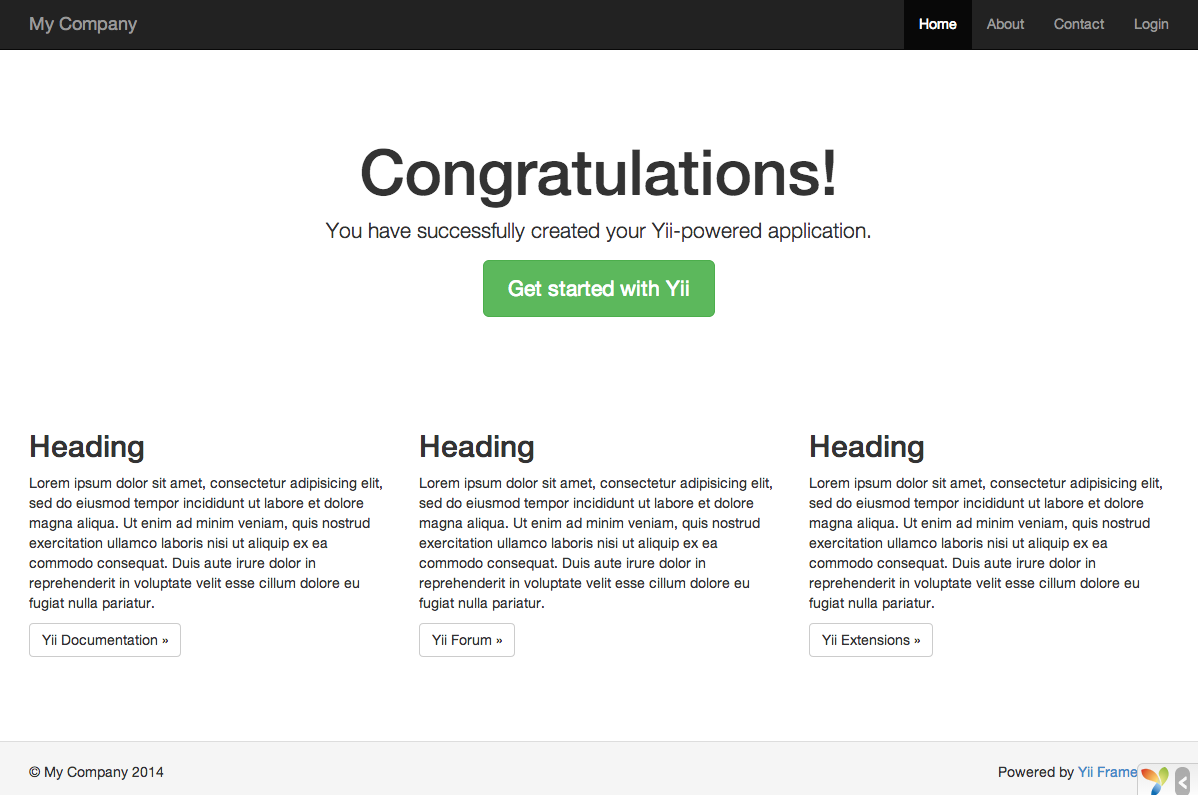
\includegraphics[width=\textwidth]{images/start-app-installed.png}

你应该可以在浏览器中看到如上所示的 “Congratulations!” 页面。如果没有,请通过以下任意一种方式,检查当前 PHP 环境是否满足 Yii 最基本需求:

\begin{itemize}
\item 通过浏览器访问 URL \lstinline|http://localhost/basic/requirements.php|
\item 执行如下命令:

\lstset{language={}}\begin{lstlisting}
cd basic
php requirements.php
\end{lstlisting}

\end{itemize}
你需要配置好 PHP 安装环境,使其符合 Yii 的最小需求。主要是需要 PHP 5.4 以上版本。如果应用需要用到数据库,那还要安装 PDO PHP 扩展\footnote{\url{http://www.php.net/manual/zh/pdo.installation.php}} 和相应的数据库驱动(例如访问 MySQL 数据库所需的 \lstinline|pdo_mysql|)。

\subsection{配置 Web 服务器 \label{start-installation.md::configuring-web-servers}}
>补充:如果你现在只是要试用 Yii 而不是将其部署到生产环境中,本小节可以跳过。

通过上述方法安装的应用程序在 Windows,Max OS X,Linux 中的 Apache HTTP 服务器\footnote{\url{http://httpd.apache.org/}}或 Nginx HTTP 服务器\footnote{\url{http://nginx.org/}}且PHP版本为5.4或更高都可以直接运行。Yii 2.0 也兼容 Facebook 公司的 HHVM\footnote{\url{http://hhvm.com/}},由于 HHVM 和标准 PHP 在边界案例上有些地方略有不同,在使用 HHVM 时需稍作处理。

在生产环境的服务器上,你可能会想配置服务器让应用程序可以通过 URL \lstinline|http://www.example.com/index.php| 访问而不是 \lstinline|http://www.example.com/basic/web/index.php|。这种配置需要将 Web 服务器的文档根目录指向 \lstinline|basic/web| 目录。可能你还会想隐藏掉 URL 中的 \lstinline|index.php|,具体细节在 \hyperref[runtime-url-handling.md]{URL 解析和生成}一章中有介绍,你将学到如何配置 Apache 或 Nginx 服务器实现这些目标。

>补充:将 \lstinline|basic/web| 设置为文档根目录,可以防止终端用户访问 \lstinline|basic/web| 相邻目录中的私有应用代码和敏感数据文件。禁止对其他目录的访问是一个不错的安全改进。

>补充:如果你的应用程序将来要运行在共享虚拟主机环境中,没有修改其 Web 服务器配置的权限,你依然可以通过调整应用的结构来提升安全性。详情请参考\hyperref[tutorial-shared-hosting.md]{共享主机环境} 一章。

\subsubsection{推荐使用的 Apache 配置 \label{start-installation.md::recommended-apache-configuration}}
在 Apache 的 \lstinline|httpd.conf| 文件或在一个虚拟主机配置文件中使用如下配置。注意,你应该将 \lstinline|path/to/basic/web| 替换为实际的 \lstinline|basic/web| 目录。

\lstset{language={}}\begin{lstlisting}
# 设置文档根目录为 “basic/web”
DocumentRoot "path/to/basic/web"

<Directory "path/to/basic/web">
    # 开启 mod_rewrite 用于美化 URL 功能的支持(译者注:对应 pretty URL 选项)
    RewriteEngine on
    # 如果请求的是真实存在的文件或目录,直接访问
    RewriteCond %{REQUEST_FILENAME} !-f
    RewriteCond %{REQUEST_FILENAME} !-d
    # 如果请求的不是真实文件或目录,分发请求至 index.php
    RewriteRule . index.php

    # ...其它设置...
</Directory>
\end{lstlisting}
\subsubsection{推荐使用的 Nginx 配置 \label{start-installation.md::recommended-nginx-configuration}}
为了使用 Nginx\footnote{\url{http://wiki.nginx.org/}},你应该已经将 PHP 安装为 FPM SAPI\footnote{\url{http://php.net/install.fpm}} 了。使用如下 Nginx 配置,将 \lstinline|path/to/basic/web| 替换为实际的 \lstinline|basic/web| 目录,\lstinline|mysite.local| 替换为实际的主机名以提供服务。

\lstset{language={}}\begin{lstlisting}
server {
    charset utf-8;
    client_max_body_size 128M;

    listen 80; ## 监听 ipv4 上的 80 端口
    #listen [::]:80 default_server ipv6only=on; ## 监听 ipv6 上的 80 端口

    server_name mysite.local;
    root        /path/to/basic/web;
    index       index.php;

    access_log  /path/to/basic/log/access.log main;
    error_log   /path/to/basic/log/error.log;

    location / {
        # 如果找不到真实存在的文件,把请求分发至 index.php
        try_files $uri $uri/ /index.php?$args;
    }

    # 若取消下面这段的注释,可避免 Yii 接管不存在文件的处理过程(404)
    #location ~ \.(js|css|png|jpg|gif|swf|ico|pdf|mov|fla|zip|rar)$ {
    #    try_files $uri =404;
    #}
    #error_page 404 /404.html;

    location ~ \.php$ {
        include fastcgi.conf;
        fastcgi_pass   127.0.0.1:9000;
        #fastcgi_pass unix:/var/run/php5-fpm.sock;
        try_files $uri =404;
    }

    location ~ /\.(ht|svn|git) {
        deny all;
    }
}
\end{lstlisting}
使用该配置时,你还应该在 \lstinline|php.ini| 文件中设置 \lstinline|cgi.fix_pathinfo=0| ,能避免掉很多不必要的 \lstinline|stat()| 系统调用。

还要注意当运行一个 HTTPS 服务器时,需要添加 \lstinline|fastcgi_param HTTPS on;| 一行,这样 Yii 才能正确地判断连接是否安全。



\label{start-workflow.md}\section{运行应用}
安装 Yii 后,就有了一个可运行的 Yii 应用,根据配置的不同,可以通过 \lstinline|http://hostname/basic/web/index.php| 或 \lstinline|http://hostname/index.php| 访问。本章节将介绍应用的内建功能,如何组织代码,以及一般情况下应用如何处理请求。

\begin{quote}补充:为简单起见,在整个“入门”板块都假定你已经把 \lstinline|basic/web| 设为 Web 服务器根目录并配置完毕,你访问应用的地址会是 \lstinline|http://lostname/index.php| 或类似的。请按需调整 URL。

\end{quote}
\subsection{功能 \label{start-workflow.md::functionality}}
一个安装完的基本应用包含四页:

\begin{itemize}
\item 主页,当你访问 \lstinline|http://hostname/index.php| 时显示,
\item “About” 页,
\item “Contact” 页, 显示一个联系表单,允许终端用户通过 Email 联系你,
\item “Login” 页, 显示一个登录表单,用来验证终端用户。试着用 “admin/admin” 登录,你可以看到当前是登录状态,已经可以“退出登录”了。
\end{itemize}
这些页面使用同一个头部和尾部。头部包含了一个可以在不同页面间切换的导航栏。

在浏览器底部可以看到一个工具栏。这是 Yii 提供的很有用的\hyperref[tool-debugger.md]{调试工具},可以记录并显示大量的调试信息,例如日志信息,响应状态,数据库查询等等。

\subsection{应用结构 \label{start-workflow.md::application-structure}}
应用中最重要的目录和文件(假设应用根目录是 \lstinline|basic|):

\lstset{language={}}\begin{lstlisting}
basic/                  应用根目录
    composer.json       Composer 配置文件, 描述包信息
    config/             包含应用配置及其它配置
        console.php     控制台应用配置信息
        web.php         Web 应用配置信息
    commands/           包含控制台命令类
    controllers/        包含控制器类
    models/             包含模型类
    runtime/            包含 Yii 在运行时生成的文件,例如日志和缓存文件
    vendor/             包含已经安装的 Composer 包,包括 Yii 框架自身
    views/              包含视图文件
    web/                Web 应用根目录,包含 Web 入口文件
        assets/         包含 Yii 发布的资源文件(javascript 和 css)
        index.php       应用入口文件
    yii                 Yii 控制台命令执行脚本
\end{lstlisting}
一般来说,应用中的文件可被分为两类:在 \lstinline|basic/web| 下的和在其它目录下的。前者可以直接通过 HTTP 访问(例如浏览器),后者不能也不应该被直接访问。

Yii 实现了模型-视图-控制器 (MVC)\footnote{\url{http://wikipedia.org/wiki/Model-view-controller}}设计模式,这点在上述目录结构中也得以体现。 \lstinline|models| 目录包含了所有\hyperref[structure-models.md]{模型类},\lstinline|views| 目录包含了所有\hyperref[structure-views.md]{视图脚本},\lstinline|controllers| 目录包含了所有\hyperref[structure-controllers.md]{控制器类}。

以下图表展示了一个应用的静态结构:

\noindent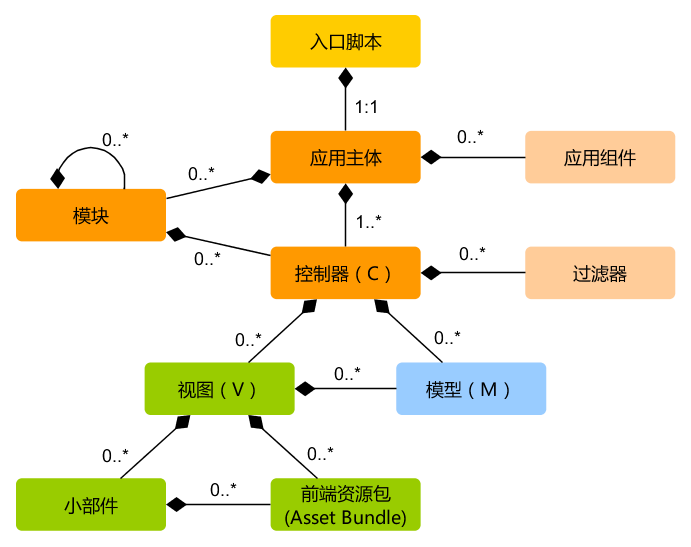
\includegraphics[width=\textwidth]{images/application-structure.png}

每个应用都有一个入口脚本 \lstinline|web/index.php|,这是整个应用中唯一可以访问的 PHP 脚本。入口脚本接受一个 Web 请求并创建\hyperref[structure-application.md]{应用}实例去处理它。 \hyperref[structure-applications.md]{应用}在它的\hyperref[concept-components.md]{组建}辅助下解析请求,并分派请求至 MVC 元素。\hyperref[structure-views.md]{视图}使用\hyperref[structure-widgets.md]{小部件}去创建复杂和动态的用户界面。

\subsection{请求生命周期 \label{start-workflow.md::request-lifecycle}}
以下图表展示了一个应用如何处理请求:

\noindent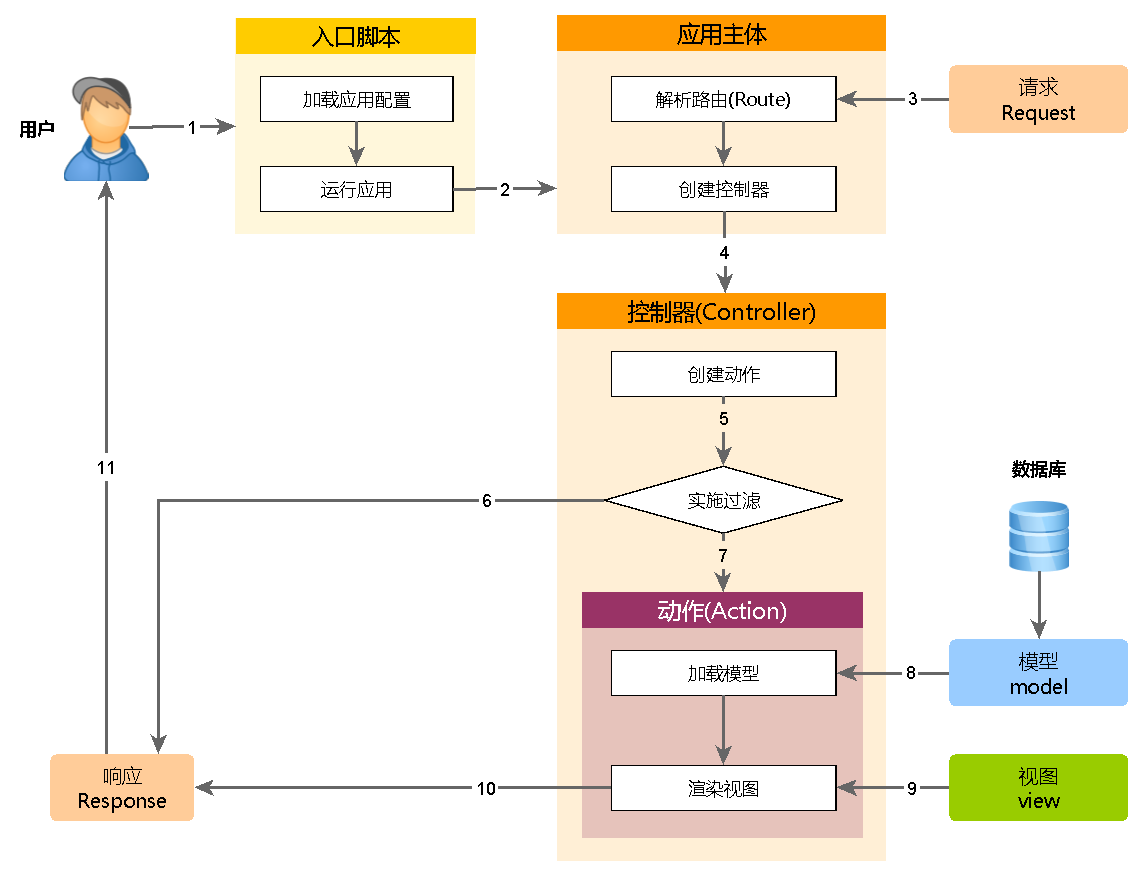
\includegraphics[width=\textwidth]{images/application-lifecycle.png}

\begin{enumerate}
\item 用户向\hyperref[structure-entry-scripts.md]{入口脚本} \lstinline|web/index.php| 发起请求。
\item 入口脚本加载应用\hyperref[concept-configurations.md]{配置}并创建一个\hyperref[structure-applications.md]{应用}实例去处理请求。
\item 应用通过\hyperref[runtime-request.md]{请求}组件解析请求的\hyperref[runtime-routing.md]{路由}。
\item 应用创建一个\hyperref[structure-controllers.md]{控制器}实例去处理请求。
\item 控制器创建一个\hyperref[structure-controllers.md]{操作}实例并针对操作执行过滤器。
\item 如果任何一个过滤器返回失败,则操作退出。
\item 如果所有过滤器都通过,操作将被执行。
\item 操作会加载一个数据模型,或许是来自数据库。
\item 操作会渲染一个视图,把数据模型提供给它。
\item 渲染结果返回给\hyperref[runtime-responses.md]{响应}组件。
\item 响应组件发送渲染结果给用户浏览器。
\end{enumerate}


\label{start-hello.md}\section{说声 Hello}
本章描述了如何在你的应用中创建一个新的 “Hello” 页面。为了实现这一目标,将会创建一个\hyperref[structure-controllers.md::creating-actions]{操作}和一个\hyperref[structure-views.md]{视图}:

\begin{itemize}
\item 应用将会分派页面请求给操作
\item 操作将会依次渲染视图呈现 “Hello” 给最终用户
\end{itemize}
贯穿整个章节,你将会掌握三件事:

\begin{enumerate}
\item 如何创建一个\hyperref[structure-controllers.md]{操作}去响应请求,
\item 如何创建一个\hyperref[structure-views.md]{视图}去构造响应内容,
\item 以及一个应用如何分派请求给\hyperref[structure-controllers.md::creating-actions]{操作}。
\end{enumerate}
\subsection{创建操作 \label{start-hello.md::creating-action}}
为了 “Hello”,需要创建一个 \lstinline|say| \hyperref[structure-controllers.md::creating-actions]{操作},从请求中接收 \lstinline|message| 参数并显示给最终用户。如果请求没有提供 \lstinline|message| 参数,操作将显示默认参数 “Hello”。

\begin{quote}补充:\hyperref[structure-controllers.md::creating-actions]{操作}是最终用户可以直接访问并执行的对象。操作被组织在\hyperref[structure-controllers.md]{控制器}中。一个操作的执行结果就是最终用户收到的响应内容。

\end{quote}
操作必须声明在\hyperref[structure-controllers.md]{控制器}中。为了简单起见,你可以直接在 \lstinline|SiteController| 控制器里声明 \lstinline|say| 操作。这个控制器是由文件 \lstinline|controllers/SiteController.php| 定义的。以下是一个操作的声明:

\lstset{language=php}\begin{lstlisting}
<?php

namespace app\controllers;

use yii\web\Controller;

class SiteController extends Controller
{
    // ...其它代码...

    public function actionSay($message = 'Hello')
    {
        return $this->render('say', ['message' => $message]);
    }
}
\end{lstlisting}
在上述 \lstinline|SiteController| 代码中,\lstinline|say| 操作被定义为 \lstinline|actionSay| 方法。Yii 使用 \lstinline|action| 前缀区分普通方法和操作。\lstinline|action| 前缀后面的名称被映射为操作的 ID。

涉及到给操作命名时,你应该理解 Yii 如何处理操作 ID。操作 ID 总是被以小写处理,如果一个操作 ID 由多个单词组成,单词之间将由连字符连接(如 \lstinline|create-comment|)。操作 ID 映射为方法名时移除了连字符,将每个单词首字母大写,并加上 \lstinline|action| 前缀。 例子:操作 ID \lstinline|create-comment| 相当于方法名 \lstinline|actionCreateComment|。

上述代码中的操作方法接受一个参数 \lstinline|$message|,它的默认值是 \lstinline|“Hello”|(就像你设置 PHP 中其它函数或方法的默认值一样)。当应用接收到请求并确定由 \lstinline|say| 操作来响应请求时,应用将从请求的参数中寻找对应值传入进来。换句话说,如果请求包含一个 \lstinline|message| 参数,它的值是 \lstinline|“Goodybye”|, 操作方法中的 \lstinline|$message| 变量也将被填充为 \lstinline|“Goodbye”|。

在操作方法中,\texttt{yii{\allowbreak{}\textbackslash}web{\allowbreak{}\textbackslash}Controller\allowbreak{}::\allowbreak{}render()} 被用来渲染一个名为 \lstinline|say| 的\hyperref[structure-views.md]{视图}文件。 \lstinline|message| 参数也被传入视图,这样就可以在里面使用。操作方法会返回渲染结果。结果会被应用接收并显示给最终用户的浏览器(作为整页 HTML 的一部分)。

\subsection{创建视图 \label{start-hello.md::creating-view}}
\hyperref[structure-views.md]{视图}是你用来生成响应内容的脚本。为了说 “Hello”,你需要创建一个 \lstinline|say| 视图,以便显示从操作方法中传来的 \lstinline|message| 参数。

\lstset{language=php}\begin{lstlisting}
<?php
use yii\helpers\Html;
?>
<?= Html::encode($message) ?>
\end{lstlisting}
\lstinline|say| 视图应该存为 \lstinline|views/site/say.php| 文件。当一个操作中调用了 \texttt{yii{\allowbreak{}\textbackslash}web{\allowbreak{}\textbackslash}Controller\allowbreak{}::\allowbreak{}render()} 方法时,它将会按 \lstinline|views/控制器 ID/视图名.php| 路径加载 PHP 文件。

注意以上代码,\lstinline|message| 参数在输出之前被 \texttt{yii{\allowbreak{}\textbackslash}helpers{\allowbreak{}\textbackslash}Html\allowbreak{}::\allowbreak{}encode()} 方法处理过。这很有必要,当参数来自于最终用户时,参数中可能隐含的恶意 JavaScript 代码会导致跨站脚本(XSS)攻击\footnote{\url{http://en.wikipedia.org/wiki/Cross-site\_scripting}}。

当然了,你大概会在 \lstinline|say| 视图里放入更多内容。内容可以由 HTML 标签,纯文本,甚至 PHP 语句组成。实际上 \lstinline|say| 视图就是一个由 \texttt{yii{\allowbreak{}\textbackslash}web{\allowbreak{}\textbackslash}Controller\allowbreak{}::\allowbreak{}render()} 执行的 PHP 脚本。视图脚本输出的内容将会作为响应结果返回给应用。应用将依次输出结果给最终用户。

\subsection{试运行 \label{start-hello.md::trying-it-out}}
创建完操作和视图后,你就可以通过下面的 URL 访问新页面了:

\lstset{language={}}\begin{lstlisting}
http://hostname/index.php?r=site/say&message=Hello+World
\end{lstlisting}
\noindent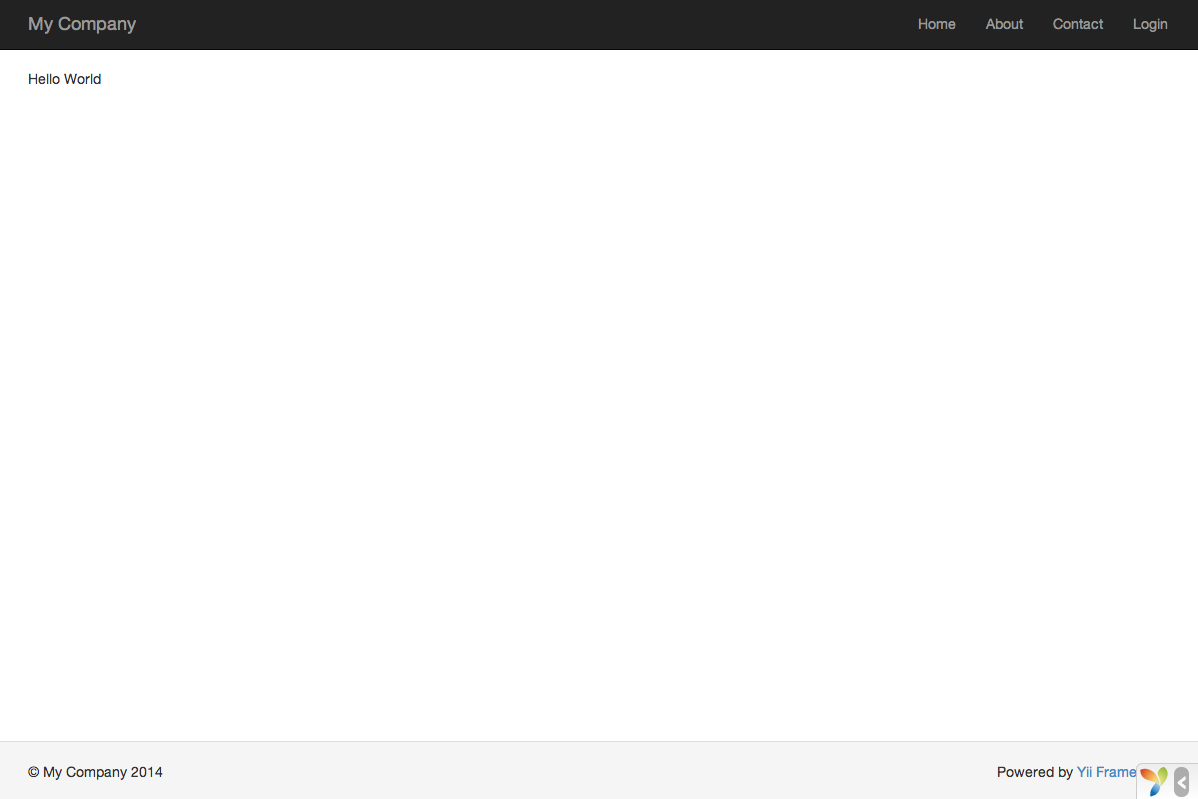
\includegraphics[width=\textwidth]{images/start-hello-world.png}

这个 URL 将会输出包含 “Hello World” 的页面,页面和应用里的其它页面使用同样的头部和尾部。

如果你省略 URL 中的 \lstinline|message| 参数,将会看到页面只显示 “Hello”。这是因为 \lstinline|message| 被作为一个参数传给 \lstinline|actionSay()| 方法,当省略它时,参数将使用默认的 \lstinline|“Hello”| 代替。

\begin{quote}补充:新页面和其它页面使用同样的头部和尾部是因为 \texttt{yii{\allowbreak{}\textbackslash}web{\allowbreak{}\textbackslash}Controller\allowbreak{}::\allowbreak{}render()} 方法会自动把 \lstinline|say| 视图执行的结果嵌入称为\hyperref[structure-views.md::layouts]{布局}的文件中,本例中是 \lstinline|views/layouts/main.php|。

\end{quote}
上面 URL 中的参数 \lstinline|r| 需要更多解释。它代表\hyperref[runtime-routing.md]{路由},是整个应用级的,指向特定操作的独立 ID。路由格式是 \lstinline|控制器 ID/操作 ID|。应用接受请求的时候会检查参数,使用控制器 ID 去确定哪个控制器应该被用来处理请求。然后相应控制器将使用操作 ID 去确定哪个操作方法将被用来做具体工作。上述例子中,路由 \lstinline|site/say| 将被解析至 \lstinline|SiteController| 控制器和其中的 \lstinline|say| 操作。因此 \lstinline|SiteController::actionSay()| 方法将被调用处理请求。

\begin{quote}补充:与操作一样,一个应用中控制器同样有唯一的 ID。控制器 ID 和操作 ID 使用同样的命名规则。控制器的类名源自于控制器 ID,移除了连字符,每个单词首字母大写,并加上 \lstinline|Controller| 后缀。例子:控制器 ID \lstinline|post-comment| 相当于控制器类名 \lstinline|PostCommentController|。

\end{quote}
\subsection{总结 \label{start-hello.md::summary}}
通过本章节你接触了 MVC 设计模式中的控制器和视图部分。创建了一个操作作为控制器的一部分去处理特定请求。然后又创建了一个视图去构造响应内容。在这个小例子中,没有模型调用,唯一涉及到数据的地方是 \lstinline|message| 参数。

你同样学习了 Yii 路由的相关内容,它是用户请求与控制器操作之间的桥梁。

下一章,你将学习如何创建一个模型,以及添加一个包含 HTML 表单的页面。



\label{start-forms.md}\section{使用表单}
本章将介绍如何创建一个从用户那搜集数据的表单页。该页将显示一个包含 name 输入框和 email 输入框的表单。当搜集完这两部分信息后,页面将会显示用户输入的信息。

为了实现这个目标,除了创建一个\hyperref[structure-controllers.md]{操作}和两个\hyperref[structure-views]{视图}外,还需要创建一个\hyperref[structure-models.md]{模型}。

贯穿整个小节,你将会学到:

\begin{itemize}
\item 创建一个\hyperref[structure-models.md]{模型}代表用户通过表单输入的数据
\item 声明规则去验证输入的数据
\item 在\hyperref[structure-views.md]{视图}中生成一个 HTML 表单
\end{itemize}
\subsection{创建模型 \label{start-forms.md::creating-model}}
模型类 \lstinline|EntryForm| 代表从用户那请求的数据,该类如下所示并存储在 \lstinline|models/EntryForm.php| 文件中。请参考\hyperref[concept-autoloading.md]{类自动加载}章节获取更多关于类命名约定的介绍。

\lstset{language=php}\begin{lstlisting}
<?php

namespace app\models;

use yii\base\Model;

class EntryForm extends Model
{
    public $name;
    public $email;

    public function rules()
    {
        return [
            [['name', 'email'], 'required'],
            ['email', 'email'],
        ];
    }
}
\end{lstlisting}
该类继承自 \texttt{yii{\allowbreak{}\textbackslash}base{\allowbreak{}\textbackslash}Model},Yii 提供的一个基类,通常用来代表表单数据。

\begin{quote}补充:\texttt{yii{\allowbreak{}\textbackslash}base{\allowbreak{}\textbackslash}Model} 被用于普通模型类的父类并与数据表\textbf{无关}。\texttt{yii{\allowbreak{}\textbackslash}db{\allowbreak{}\textbackslash}ActiveRecord} 通常是普通模型类的父类但与数据表有关联。

\end{quote}
\lstinline|EntryForm| 类包含 \lstinline|name| 和 \lstinline|email| 两个公共变量,用来储存用户输入的数据。它还包含一个名为 \lstinline|rules()| 的方法,用来返回数据验证规则的集合。上面声明的验证规则表示:

\begin{itemize}
\item \lstinline|name| 和 \lstinline|email| 值都是必须的
\item \lstinline|mail| 的值必须满足 email 地址验证
\end{itemize}
如果你有一个从用户那搜集数据的 \lstinline|EntryForm| 对象,你可以调用它的 \texttt{yii{\allowbreak{}\textbackslash}base{\allowbreak{}\textbackslash}Model\allowbreak{}::\allowbreak{}validate()} 方法触发数据验证。如果有数据验证失败,将把 \texttt{yii{\allowbreak{}\textbackslash}base{\allowbreak{}\textbackslash}Model\allowbreak{}::\allowbreak{}hasErrors} 属性设为 ture,想要知道具体发生什么错误就调用 \texttt{yii{\allowbreak{}\textbackslash}base{\allowbreak{}\textbackslash}Model\allowbreak{}::\allowbreak{}getErrors}。

\lstset{language=php}\begin{lstlisting}
<?php
$model = new EntryForm();
$model->name = 'Qiang';
$model->email = 'bad';
if ($model->validate()) {
    // 验证成功!
} else {
    // 失败!
    // 使用 $model->getErrors() 获取错误详情
}
\end{lstlisting}
\subsection{创建操作 \label{start-forms.md::creating-action}}
接下来你需要在 \lstinline|site| 控制器中创建一个 \lstinline|entry| 操作用于新建的模型。操作的创建和使用已经在\hyperref[start-hello.md]{说一声你好}小节中解释了。

\lstset{language=php}\begin{lstlisting}
<?php

namespace app\controllers;

use Yii;
use yii\web\Controller;
use app\models\EntryForm;

class SiteController extends Controller
{
    // ...其它代码...

    public function actionEntry()
    {
        $model = new EntryForm;

        if ($model->load(Yii::$app->request->post()) && $model->validate()) {
            // 验证 $model 收到的数据

            // 做些有意义的事 ...

            return $this->render('entry-confirm', ['model' => $model]);
        } else {
            // 无论是初始化显示还是数据验证错误
            return $this->render('entry', ['model' => $model]);
        }
    }
}
\end{lstlisting}
该操作首先创建了一个 \lstinline|EntryForm| 对象。然后尝试从 \lstinline|$_POST| 搜集用户提交的数据,由 Yii 的 \texttt{yii{\allowbreak{}\textbackslash}web{\allowbreak{}\textbackslash}Request\allowbreak{}::\allowbreak{}post()} 方法负责搜集。如果模型被成功填充数据(也就是说用户已经提交了 HTML 表单),操作将调用 \texttt{yii{\allowbreak{}\textbackslash}base{\allowbreak{}\textbackslash}Model\allowbreak{}::\allowbreak{}validate()} 去确保用户提交的是有效数据。

\begin{quote}补充:表达式 \lstinline|Yii::$app| 代表\hyperref[structure-applications.md]{应用}实例,它是一个全局可访问的单例。同时它也是一个\hyperref[concept-service-locator.md]{服务定位器},能提供 \lstinline|request|,\lstinline|response|,\lstinline|db| 等等特定功能的组件。在上面的代码里就是使用 \lstinline|request| 组件来访问应用实例收到的 \lstinline|$_POST| 数据。

\end{quote}
用户成功提交表单后,操作将会渲染一个名为 \lstinline|entry-confirm| 的视图去确认用户输入的数据。如果没填表单就提交,或数据包含错误,\lstinline|entry| 视图将会渲染输出,连同表单一起输出的还有验证错误的详细信息。

\begin{quote}注意:在这个简单例子里我们只是呈现了有效数据的确认页面。实践中你应该考虑使用 \texttt{yii{\allowbreak{}\textbackslash}web{\allowbreak{}\textbackslash}Controller\allowbreak{}::\allowbreak{}refresh()} 或 \texttt{yii{\allowbreak{}\textbackslash}web{\allowbreak{}\textbackslash}Controller\allowbreak{}::\allowbreak{}redirect()} 去避免表单重复提交问题\footnote{\url{http://en.wikipedia.org/wiki/Post/Redirect/Get}}。

\end{quote}
\subsection{创建视图 \label{start-forms.md::creating-views}}
最后创建两个视图文件 \lstinline|entry-confirm| 和 \lstinline|entry|。他们会被刚才创建的 \lstinline|entry| 操作渲染。

\lstinline|entry-confirm| 视图简单地显示提交的 name 和 email 数据。视图文件保存在 \lstinline|views/site/entry-confirm.php|。

\lstset{language=php}\begin{lstlisting}
<?php
use yii\helpers\Html;
?>
<p>You have entered the following information:</p>

<ul>
    <li><label>Name</label>: <?= Html::encode($model->name) ?></li>
    <li><label>Email</label>: <?= Html::encode($model->email) ?></li>
</ul>
\end{lstlisting}
\lstinline|entry| 视图显示一个 HTML 表单。视图文件保存在 \lstinline|views/site/entry.php|。

\lstset{language=php}\begin{lstlisting}
<?php
use yii\helpers\Html;
use yii\widgets\ActiveForm;
?>
<?php $form = ActiveForm::begin(); ?>

    <?= $form->field($model, 'name') ?>

    <?= $form->field($model, 'email') ?>

    <div class="form-group">
        <?= Html::submitButton('Submit', ['class' => 'btn btn-primary']) ?>
    </div>

<?php ActiveForm::end(); ?>
\end{lstlisting}
视图使用了一个功能强大的\hyperref[structure-widgets.md]{小部件} \texttt{yii{\allowbreak{}\textbackslash}widgets{\allowbreak{}\textbackslash}ActiveForm} 去生成 HTML 表单。其中的 \lstinline|begin()| 和 \lstinline|end()| 分别用来渲染表单的开始和关闭标签。在这两个方法之间使用了 \texttt{yii{\allowbreak{}\textbackslash}widgets{\allowbreak{}\textbackslash}ActiveForm\allowbreak{}::\allowbreak{}field()} 方法去创建表单栏。第一个表单栏用于 “name”,第二个表单栏用于 “email”。之后使用 \texttt{yii{\allowbreak{}\textbackslash}helpers{\allowbreak{}\textbackslash}Html\allowbreak{}::\allowbreak{}submitButton()} 方法生成提交按钮。

\subsection{试运行 \label{start-forms.md::trying-it-out}}
用浏览器访问下面的 URL 看它能否工作:

\lstset{language={}}\begin{lstlisting}
http://hostname/index.php?r=site/entry
\end{lstlisting}
你会看到一个包含两个表单栏的页面。每个表单栏的前面都有一个标签指明应该输入的数据类型。如果什么都不填就点击提交按钮,或填入格式不正确的 email 地址,将会看到在对应的表单栏下显示错误信息。

\noindent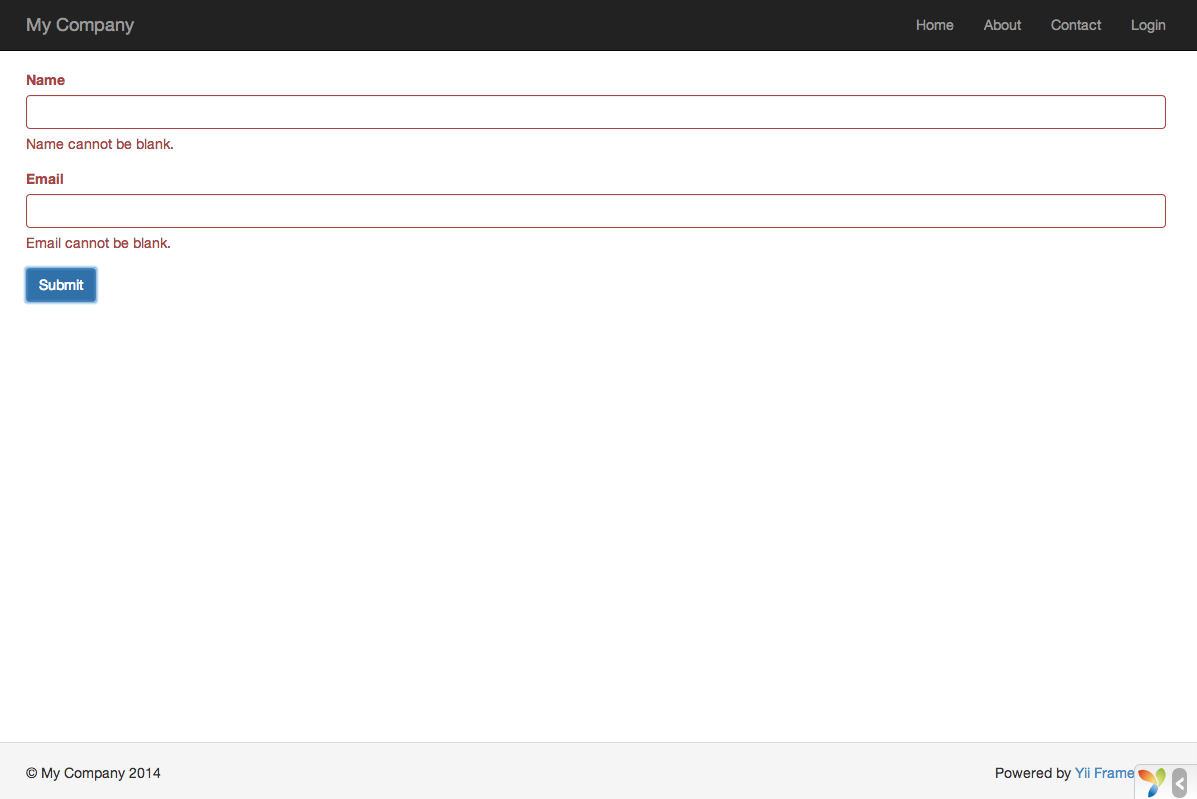
\includegraphics[width=\textwidth]{images/start-form-validation.png}

输入有效的 name 和 email 信息并提交后,将会看到一个显示你所提交数据的确认页面。

\noindent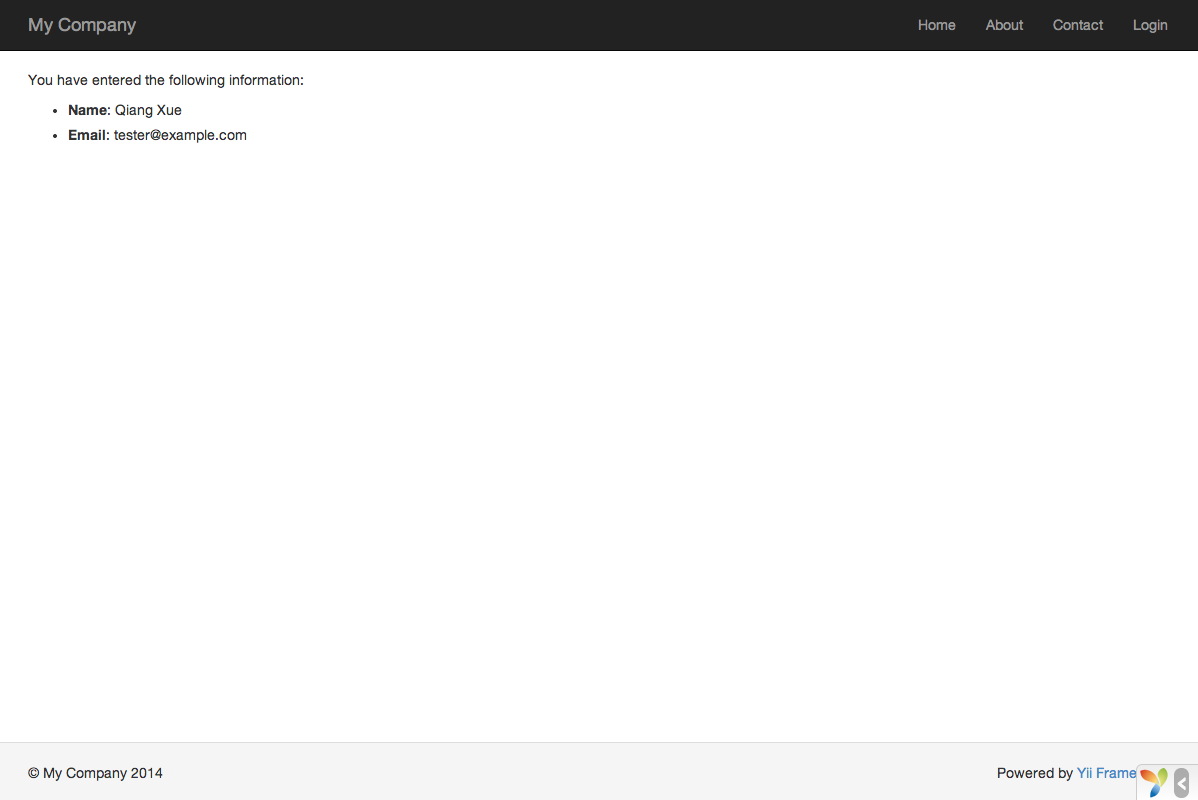
\includegraphics[width=\textwidth]{images/start-entry-confirmation.png}

\subsubsection{效果说明 \label{start-forms.md::magic-explained}}
你可能会好奇 HTML 表单暗地里是如何工作的,看起来它可以为每个表单栏显示文字标签,而当你没输入正确的信息时又不需要刷新页面就能给出错误提示,似乎有些神奇。

是的,其实数据首先由客户端 JavaScript 脚本验证,然后才会提交给服务器通过 PHP 验证。\texttt{yii{\allowbreak{}\textbackslash}widgets{\allowbreak{}\textbackslash}ActiveForm} 足够智能到把你在 \lstinline|EntryForm| 模型中声明的验证规则转化成客户端 JavaScript 脚本去执行验证。如果用户浏览器禁用了 JavaScript, 服务器端仍然会像 \lstinline|actionEntry()| 方法里这样验证一遍数据。这保证了任何情况下用户提交的数据都是有效的。

\begin{quote}警告:客户端验证只是提高用户体验的手段。无论它是否正常启用,服务端验证则都是必须的,请不要忽略它。

\end{quote}
表单栏的文字标签是 \lstinline|field()| 方法生成的,内容就是模型中该数据的属性名。例如模型中的 \lstinline|name| 属性生成的标签就是 \lstinline|Name|。

你可以在视图中自定义标签:

\lstset{language=php}\begin{lstlisting}
<?= $form->field($model, 'name')->label('自定义 Name') ?>
<?= $form->field($model, 'email')->label('自定义 Email') ?>
\end{lstlisting}
\begin{quote}补充:Yii 提供了相当多类似的小部件去帮你生成复杂且动态的视图。在后面你还会了解到自己写小部件是多么简单。你可能会把自己的很多视图代码转化成小部件以提高重用,加快开发效率。

\end{quote}
\subsection{总结 \label{start-forms.md::summary}}
本章指南中你接触了 MVC 设计模式的每个部分。学到了如何创建一个模型代表用户数据并验证它的有效性。

你还学到了如何从用户那获取数据并在浏览器上回显给用户。这本来是开发应用的过程中比较耗时的任务,好在 Yii 提供了强大的小部件让它变得如此简单。

下一章你将学习如何使用数据库,几乎每个应用都需要数据库。



\label{start-databases.md}\section{使用数据库}
本章节将介绍如何如何创建一个从数据表 \lstinline|country| 中读取国家数据并显示出来的页面。为了实现这个目标,你将会配置一个数据库连接,创建一个\hyperref[db-active-record.md]{活动记录}类,并且创建一个\hyperref[structure-controllers.md]{操作}及一个\hyperref[structure-views.md]{视图}。

贯穿整个章节,你将会学到:

\begin{itemize}
\item 配置一个数据库连接
\item 定义一个活动记录类
\item 使用活动记录从数据库中查询数据
\item 以分页方式在视图中显示数据
\end{itemize}
请注意,为了掌握本章你应该具备最基本的数据库知识和使用经验。尤其是应该知道如何创建数据库,如何通过数据库终端执行 SQL 语句。

\subsection{准备数据库 \label{start-databases.md::preparing-database}}
首先创建一个名为 \lstinline|yii2basic| 的数据库,应用将从这个数据库中读取数据。你可以创建 SQLite,MySQL,PostregSQL,MSSQL 或 Oracle 数据库,Yii 内置多种数据库支持。简单起见,后面的内容将以 MySQL 为例做演示。

然后在数据库中创建一个名为 \lstinline|country| 的表并插入简单的数据。可以执行下面的语句:

\lstset{language=sql}\begin{lstlisting}
CREATE TABLE `country` (
  `code` CHAR(2) NOT NULL PRIMARY KEY,
  `name` CHAR(52) NOT NULL,
  `population` INT(11) NOT NULL DEFAULT '0'
) ENGINE=InnoDB DEFAULT CHARSET=utf8;

INSERT INTO `country` VALUES ('AU','Australia',18886000);
INSERT INTO `country` VALUES ('BR','Brazil',170115000);
INSERT INTO `country` VALUES ('CA','Canada',1147000);
INSERT INTO `country` VALUES ('CN','China',1277558000);
INSERT INTO `country` VALUES ('DE','Germany',82164700);
INSERT INTO `country` VALUES ('FR','France',59225700);
INSERT INTO `country` VALUES ('GB','United Kingdom',59623400);
INSERT INTO `country` VALUES ('IN','India',1013662000);
INSERT INTO `country` VALUES ('RU','Russia',146934000);
INSERT INTO `country` VALUES ('US','United States',278357000);
\end{lstlisting}
此时便有了一个名为 \lstinline|yii2basic| 的数据库,在这个数据库中有一个包含三个字段的数据表 \lstinline|country|,表中有十行数据。

\subsection{配置数据库连接 \label{start-databases.md::configuring-db-connection}}
开始之前,请确保你已经安装了 PHP PDO\footnote{\url{http://www.php.net/manual/en/book.pdo.php}} 扩展和你所使用的数据库的 PDO 驱动(例如 MySQL 的 \lstinline|pdo_mysql|)。对于使用关系型数据库来讲,这是基本要求。

驱动和扩展安装可用后,打开 \lstinline|config/db.php| 修改里面的配置参数对应你的数据库配置。该文件默认包含这些内容:

\lstset{language=php}\begin{lstlisting}
<?php

return [
    'class' => 'yii\db\Connection',
    'dsn' => 'mysql:host=localhost;dbname=yii2basic',
    'username' => 'root',
    'password' => '',
    'charset' => 'utf8',
];
\end{lstlisting}
\lstinline|config/db/php| 是一个典型的基于文件的\hyperref[concept-configurations.md]{配置}工具。这个文件配置了数据库连接 \texttt{yii{\allowbreak{}\textbackslash}db{\allowbreak{}\textbackslash}Connection} 的创建和初始化参数,应用的 SQL 查询正是基于这个数据库。

上面配置的数据库连接可以在应用中通过 \lstinline|Yii::$app->db| 表达式访问。

\begin{quote}补充:\lstinline|config/db.php| 将被包含在应用配置文件 \lstinline|config/web.php| 中,后者指定了整个\hyperref[structure-applications.md]{应用}如何初始化。请参考\hyperref[concept-configurations.md]{配置}章节了解更多信息。

\end{quote}
\subsection{创建活动记录 \label{start-databases.md::creating-active-record}}
创建一个继承自\hyperref[db-active-record.md]{活动记录}类的类 \lstinline|Country|,把它放在 \lstinline|models/Country.php| 文件,去代表和读取 \lstinline|country| 表的数据。

\lstset{language=php}\begin{lstlisting}
<?php

namespace app\models;

use yii\db\ActiveRecord;

class Country extends ActiveRecord
{
}
\end{lstlisting}
这个 \lstinline|Country| 类继承自 \texttt{yii{\allowbreak{}\textbackslash}db{\allowbreak{}\textbackslash}ActiveRecord}。你不用在里面写任何代码。只需要像现在这样,Yii 就能根据类名去猜测对应的数据表名。

\begin{quote}补充:如果类名和数据表名不能直接对应,可以覆写 \texttt{yii{\allowbreak{}\textbackslash}db{\allowbreak{}\textbackslash}ActiveRecord\allowbreak{}::\allowbreak{}tableName()} 方法去显式指定相关表名。

\end{quote}
使用 \lstinline|Country| 类可以很容易地操作 \lstinline|country| 表数据,就像这段代码:

\lstset{language=php}\begin{lstlisting}
use app\models\Country;

// 获取 country 表的所有行并以 name 排序
$countries = Country::find()->orderBy('name')->all();

// 获取主键为 “US” 的行
$country = Country::findOne('US');

// 输出 “United States”
echo $country->name;

// 修改 name 为 “U.S.A.” 并在数据库中保存更改
$country->name = 'U.S.A.';
$country->save();
\end{lstlisting}
\begin{quote}补充:活动记录是面向对象、功能强大的访问和操作数据库数据的方式。你可以在\hyperref[db-active-record.md]{活动记录}章节了解更多信息。除此之外你还可以使用另一种更原生的被称做\hyperref[db-dao]{数据访问对象}的方法操作数据库数据。

\end{quote}
\subsection{创建操作 \label{start-databases.md::creating-action}}
为了向最终用户显示国家数据,你需要创建一个操作。相比之前小节掌握的在 \lstinline|site| 控制器中创建操作,在这里为所有和国家有关的数据新建一个控制器更加合理。新控制器名为 \lstinline|CountryController|,并在其中创建一个 \lstinline|index| 操作,如下:

\lstset{language=php}\begin{lstlisting}
<?php

namespace app\controllers;

use yii\web\Controller;
use yii\data\Pagination;
use app\models\Country;

class CountryController extends Controller
{
    public function actionIndex()
    {
        $query = Country::find();

        $pagination = new Pagination([
            'defaultPageSize' => 5,
            'totalCount' => $query->count(),
        ]);

        $countries = $query->orderBy('name')
            ->offset($pagination->offset)
            ->limit($pagination->limit)
            ->all();

        return $this->render('index', [
            'countries' => $countries,
            'pagination' => $pagination,
        ]);
    }
}
\end{lstlisting}
把上面的代码保存在 \lstinline|controllers/CountryController.php| 文件中。

\lstinline|index| 操作调用了活动记录 \lstinline|Country::find()| 方法,去生成查询语句并从 \lstinline|country| 表中取回所有数据。为了限定每个请求所返回的国家数量,查询在 \texttt{yii{\allowbreak{}\textbackslash}data{\allowbreak{}\textbackslash}Pagination} 对象的帮助下进行分页。 \lstinline|Pagination| 对象的使命主要有两点:

\begin{itemize}
\item 为 SQL 查询语句设置 \lstinline|offset| 和 \lstinline|limit| 从句,确保每个请求只需返回一页数据(本例中每页是 5 行)。
\item 在视图中显示一个由页码列表组成的分页器,这点将在后面的段落中解释。
\end{itemize}
在代码末尾,\lstinline|index| 操作渲染一个名为 \lstinline|index| 的视图,并传递国家数据和分页信息进去。

\subsection{创建视图 \label{start-databases.md::creating-view}}
在 \lstinline|views| 目录下先创建一个名为 \lstinline|country| 的子目录。这个目录存储所有由 \lstinline|country| 控制器渲染的视图。在 \lstinline|views/country| 目录下创建一个名为 \lstinline|index.php| 的视图文件,内容如下:

\lstset{language=php}\begin{lstlisting}
<?php
use yii\helpers\Html;
use yii\widgets\LinkPager;
?>
<h1>Countries</h1>
<ul>
<?php foreach ($countries as $country): ?>
    <li>
        <?= Html::encode("{$country->name} ({$country->code})") ?>:
        <?= $country->population ?>
    </li>
<?php endforeach; ?>
</ul>

<?= LinkPager::widget(['pagination' => $pagination]) ?>
\end{lstlisting}
这个视图包含两部分用以显示国家数据。第一部分遍历国家数据并以无序 HTML 列表渲染出来。第二部分使用 \texttt{yii{\allowbreak{}\textbackslash}widgets{\allowbreak{}\textbackslash}LinkPager} 去渲染从操作中传来的分页信息。小部件 \lstinline|LinkPager| 显示一个分页按钮的列表。点击任何一个按钮都会跳转到对应的分页。

\subsection{试运行 \label{start-databases.md::trying-it-out}}
浏览器访问下面的 URL 看看能否工作:

\lstset{language={}}\begin{lstlisting}
http://hostname/index.php?r=country/index
\end{lstlisting}
\noindent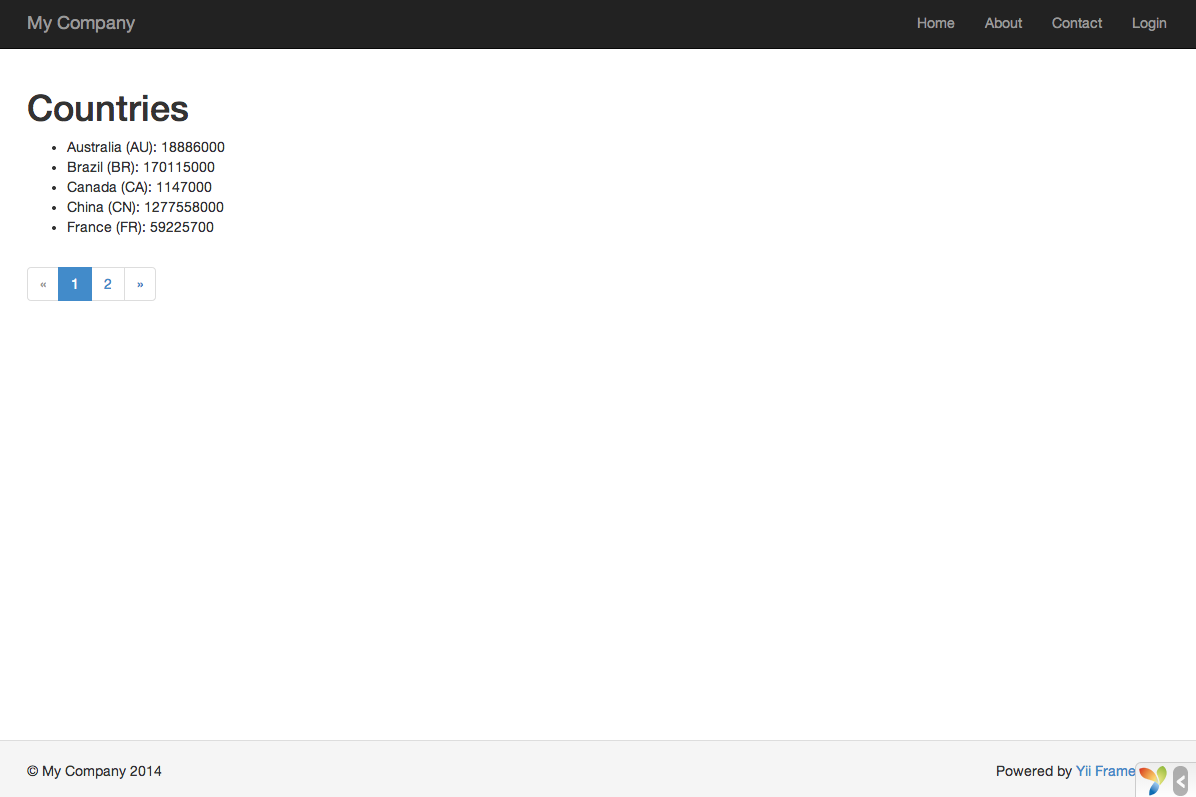
\includegraphics[width=\textwidth]{images/start-country-list.png}

首先你会看到显示着五个国家的列表页面。在国家下面,你还会看到一个包含四个按钮的分页器。如果你点击按钮 “2”,将会跳转到显示另外五个国家的页面,也就是第二页记录。如果观察仔细点你还会看到浏览器的 URL 变成了:

\lstset{language={}}\begin{lstlisting}
http://hostname/index.php?r=country/index&page=2
\end{lstlisting}
在这个场景里,\texttt{yii{\allowbreak{}\textbackslash}data{\allowbreak{}\textbackslash}Pagination} 提供了为数据结果集分页的所有功能:

\begin{itemize}
\item 首先 \texttt{yii{\allowbreak{}\textbackslash}data{\allowbreak{}\textbackslash}Pagination} 把 SELECT 的子查询 \lstinline|LIMIT 5 OFFSET 0| 数据表示成第一页。因此开头的五条数据会被取出并显示。
\item 然后小部件 \texttt{yii{\allowbreak{}\textbackslash}widgets{\allowbreak{}\textbackslash}LinkPager} 使用 \texttt{yii{\allowbreak{}\textbackslash}data{\allowbreak{}\textbackslash}Pagination\allowbreak{}::\allowbreak{}createUrl()} 方法生成的 URL 去渲染翻页按钮。URL 中包含必要的参数 \lstinline|page| 才能查询不同的页面编号。
\item 如果你点击按钮 “2”,将会发起一个路由为 \lstinline|country/index| 的新请求。\texttt{yii{\allowbreak{}\textbackslash}data{\allowbreak{}\textbackslash}Pagination} 接收到 URL 中的 \lstinline|page| 参数把当前的页码设为 2。新的数据库请求将会以 \lstinline|LIMIT 5 OFFSET 5| 查询并显示。
\end{itemize}
\subsection{总结 \label{start-databases.md::summary}}
本章节中你学到了如何使用数据库。你还学到了如何取出并使用 \texttt{yii{\allowbreak{}\textbackslash}data{\allowbreak{}\textbackslash}Pagination} 和 \texttt{yii{\allowbreak{}\textbackslash}widgets{\allowbreak{}\textbackslash}LinkPager} 显示数据。

下一章中你会学到如何使用 Yii 中强大的代码生成器 \hyperref[tool-gii.md]{Gii},去帮助你实现一些常用的功能需求,例如增查改删(CRUD)数据表中的数据。事实上你之前所写的代码全部都可以由 Gii 自动生成。



\label{start-gii.md}\section{使用 Gii 生成代码}
本章将介绍如何使用 \hyperref[tool-gii.md]{Gii} 去自动生成 Web 站点常用功能的代码。使用 Gii 生成代码非常简单,只要按照 Gii 页面上的介绍输入正确的信息即可。

贯穿本章节,你将会学到:

\begin{itemize}
\item 在你的应用中开启 Gii
\item 使用 Gii 去生成活动记录类
\item 使用 Gii 去生成数据表操作的增查改删(CRUD)代码
\item 自定义 Gii 生成的代码
\end{itemize}
\subsection{开始 Gii \label{start-gii.md::starting-gii}}
\hyperref[tool-gii.md]{Gii} 是 Yii 中的一个\hyperref[structure-modules.md]{模块}。可以通过配置应用的 \texttt{yii{\allowbreak{}\textbackslash}base{\allowbreak{}\textbackslash}Application\allowbreak{}::\allowbreak{}modules} 属性开启它。通常来讲在 \lstinline|config/web.php| 文件中会有以下配置代码:

\lstset{language=php}\begin{lstlisting}
$config = [ ... ];

if (YII_ENV_DEV) {
    $config['bootstrap'][] = 'gii';
    $config['modules']['gii'] = 'yii\gii\Module';
}
\end{lstlisting}
这段配置表明,如果当前是\hyperref[concept-configurations.md::environment-constants]{开发环境},应用会包含 \lstinline|gii| 模块,模块类是 \texttt{yii{\allowbreak{}\textbackslash}gii{\allowbreak{}\textbackslash}Module}。

如果你检查应用的\hyperref[structure-entry-scripts.md]{入口脚本} \lstinline|web/index.php|,将看到这行代码将 \lstinline|YII_ENV_DEV| 设为 true:

\lstset{language=php}\begin{lstlisting}
defined('YII_ENV') or define('YII_ENV', 'dev');
\end{lstlisting}
鉴于这行代码的定义,应用处于开发模式下,按照上面的配置会打开 Gii 模块。你可以直接通过 URL 访问 Gii:

\lstset{language={}}\begin{lstlisting}
http://hostname/index.php?r=gii
\end{lstlisting}
\begin{quote}补充: 如果你通过本机以外的机器访问 Gii,请求会被出于安全原因拒绝。你可以配置 Gii 为其添加允许访问的 IP 地址:

\lstset{language=php}\begin{lstlisting}
'gii' => [
    'class' => 'yii\gii\Module',
    'allowedIPs' => ['127.0.0.1', '::1', '192.168.0.*', '192.168.178.20'] // 按需调整这里
],
\end{lstlisting}
\end{quote}
\noindent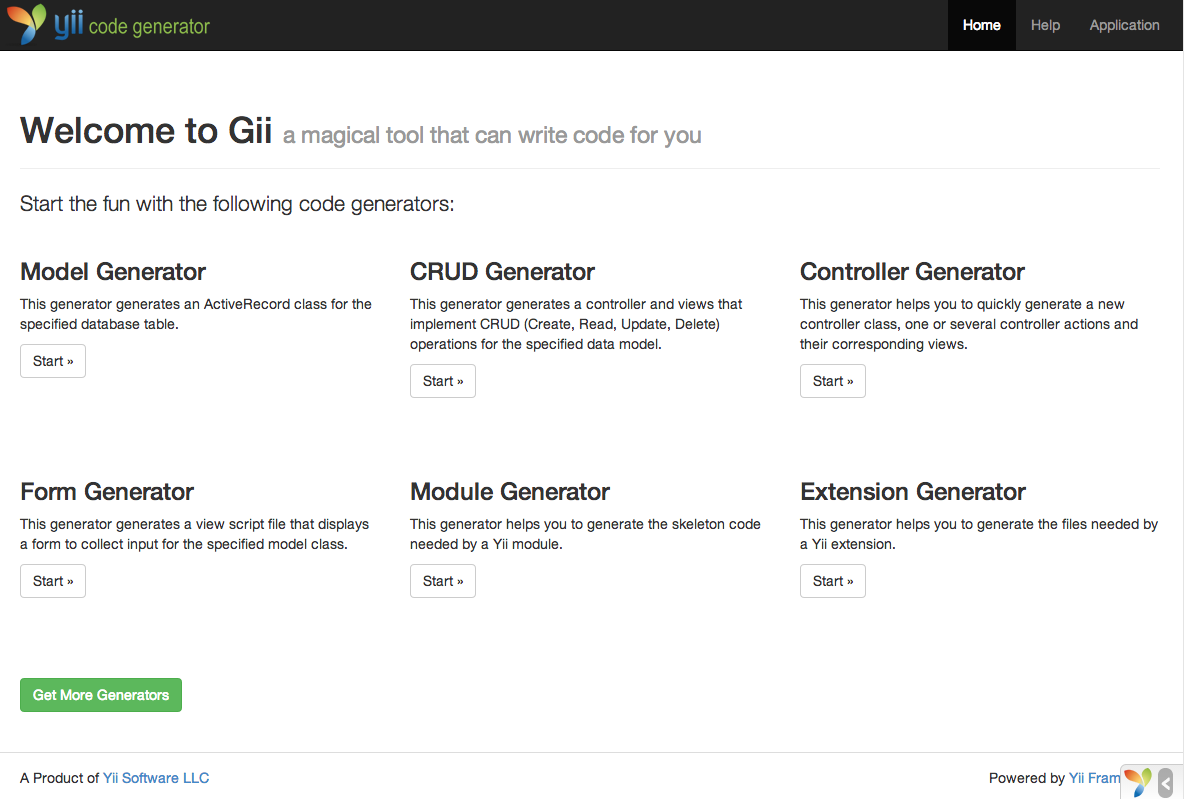
\includegraphics[width=\textwidth]{images/start-gii.png}

\subsection{生成活动记录类 \label{start-gii.md::generating-ar}}
选择 “Model Generator” (点击 Gii 首页的链接)去生成活动记录类。并像这样填写表单:

\begin{itemize}
\item Table Name: \lstinline|country|
\item Model Class: \lstinline|Country|
\end{itemize}
\noindent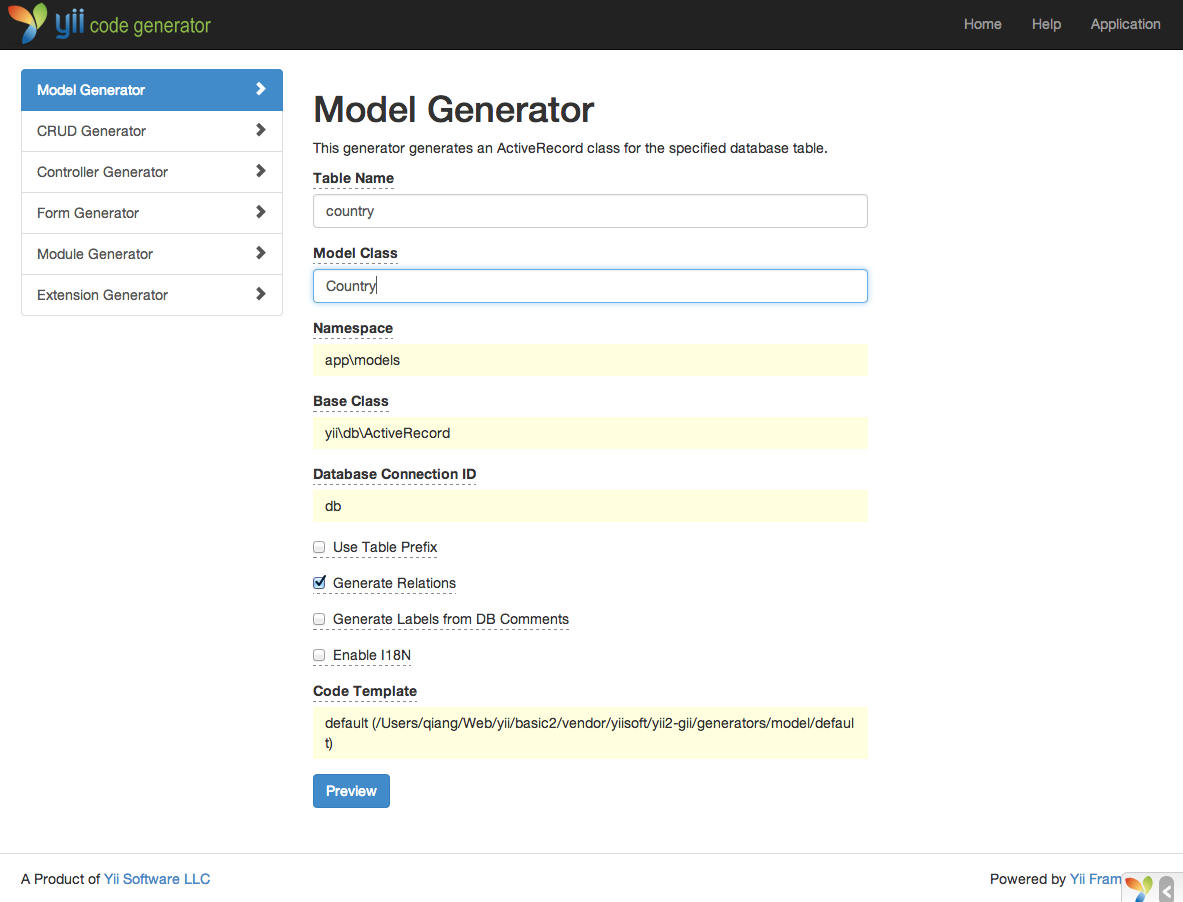
\includegraphics[width=\textwidth]{images/start-gii-model.png}

然后点击 “Preview” 按钮。你会看到 \lstinline|models/Country.php| 被列在将要生成的文件列表中。可以点击文件名预览内容。

如果你已经创建过同样的文件,使用 Gii 会覆写它,点击文件名旁边的 \lstinline|diff| 能查看现有文件与将要生成的文件的内容区别。

\noindent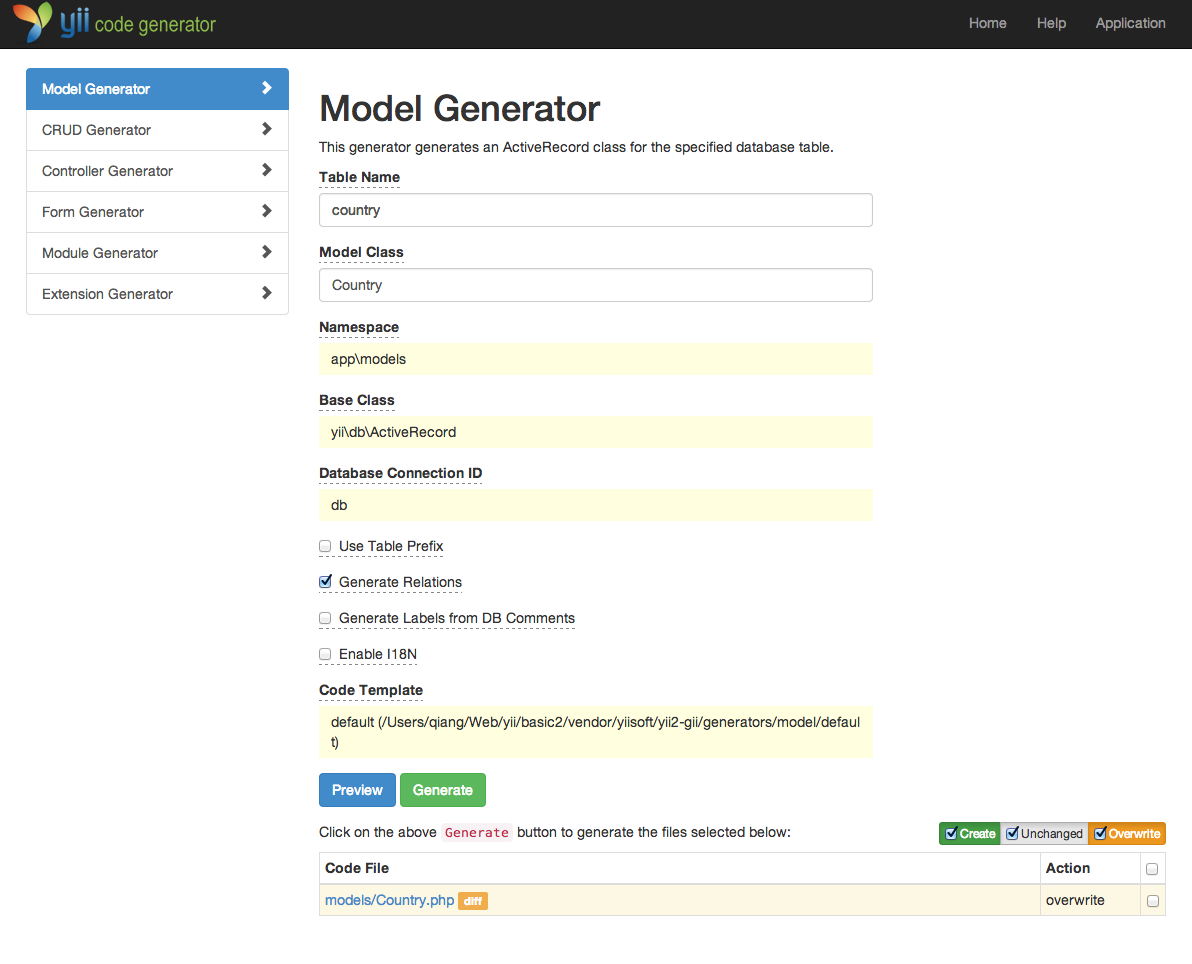
\includegraphics[width=\textwidth]{images/start-gii-model-preview.png}

想要覆写已存在文件,选中 “overwrite” 下的复选框然后点击 “Generator”。如果是新文件,只点击 “Generator” 就好。

接下来你会看到一个包含已生成文件的说明页面。如果生成过程中覆写过文件,还会有一条信息说明代码是重新生成覆盖的。

\subsection{生成 CRUD 代码 \label{start-gii.md::generating-crud}}
CRUD 代表增,查,改,删操作,这是绝大多数 Web 站点常用的数据处理方式。选择 Gii 中的 “CRUD Generator” (点击 Gii 首页的链接)去创建 CRUD 功能。本例 “country” 中需要这样填写表单:

\begin{itemize}
\item Model Class: \lstinline|app\models\Country|
\item Search Model Class: \lstinline|app\models\CountrySearch|
\item Controller Class: \lstinline|app\controllers\CountryController|
\end{itemize}
\noindent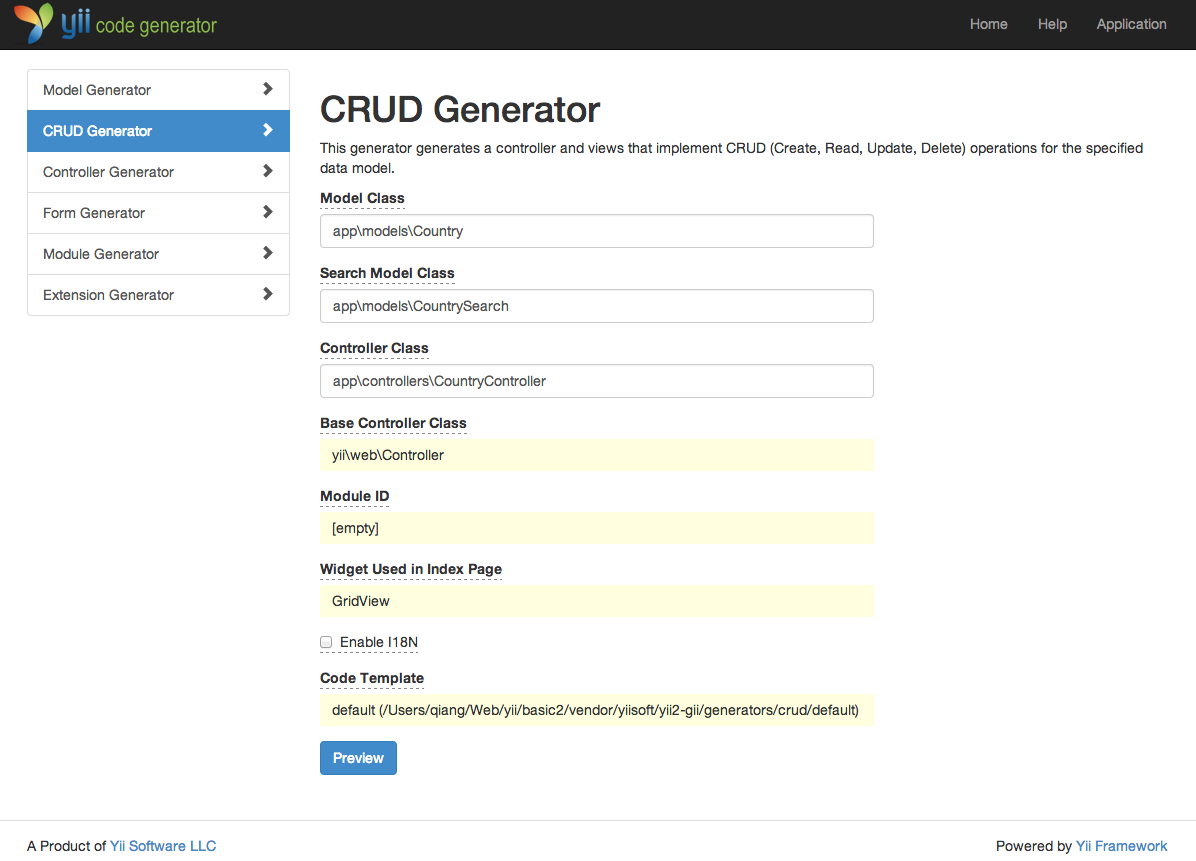
\includegraphics[width=\textwidth]{images/start-gii-crud.png}

然后点击 “Preview” 按钮。你会看到下述将要生成的文件列表。

[[NEED THE IMAGE HERE / 等待官方补充图片]]

如果你之前创建过 \lstinline|controllers/CountryController.php| 和 \lstinline|views/country/index.php| 文件(在指南的使用数据库章节),选中 “overwrite” 下的复选框覆写它们(之前的文件没能全部支持 CRUD)。

\subsection{试运行 \label{start-gii.md::trying-it-out}}
用浏览器访问下面的 URL 查看生成代码的运行:

\lstset{language={}}\begin{lstlisting}
http://hostname/index.php?r=country/index
\end{lstlisting}
可以看到一个栅格显示着从数据表中读取的国家数据。支持在列头对数据进行排序,输入筛选条件进行筛选。

可以浏览详情,编辑,或删除栅格中的每个国家。还可以点击栅格上方的 “Create Country” 按钮通过表单创建新国家。

\noindent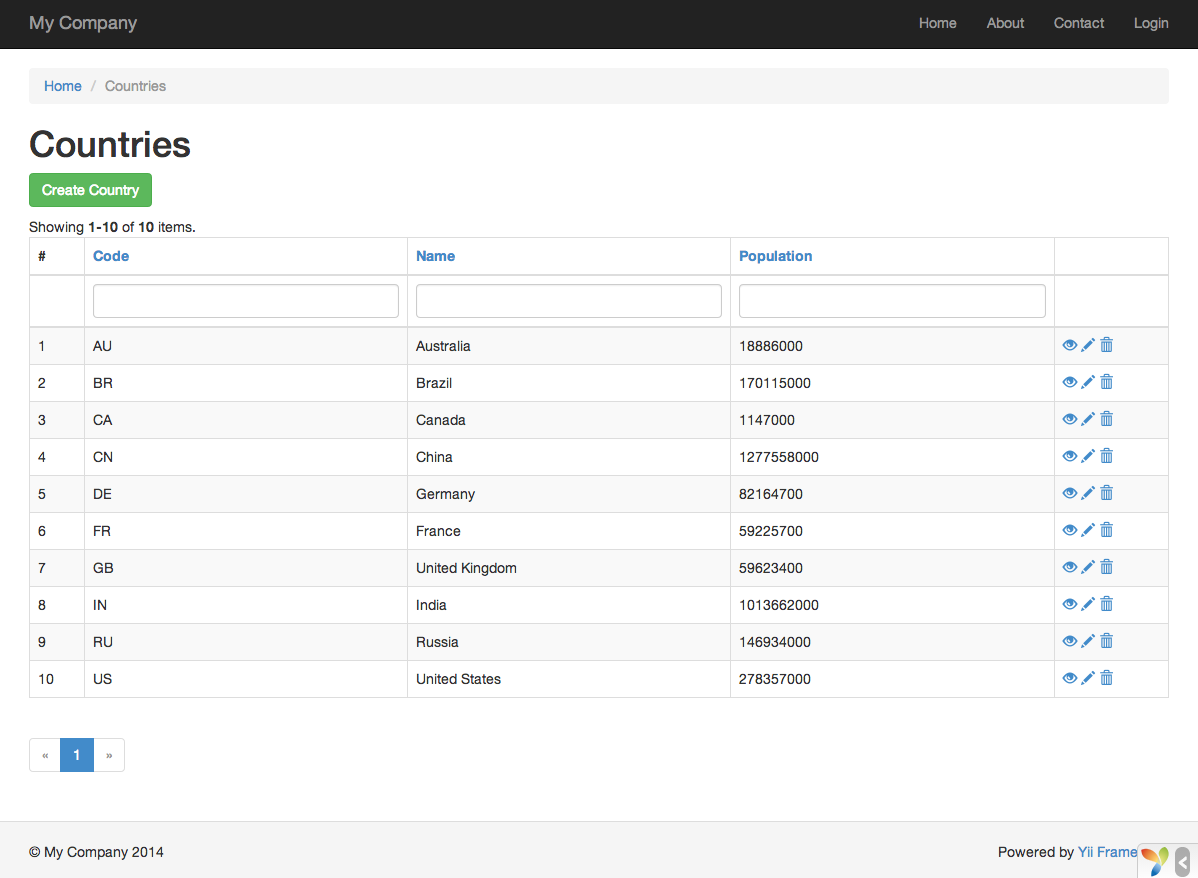
\includegraphics[width=\textwidth]{images/start-gii-country-grid.png}

\noindent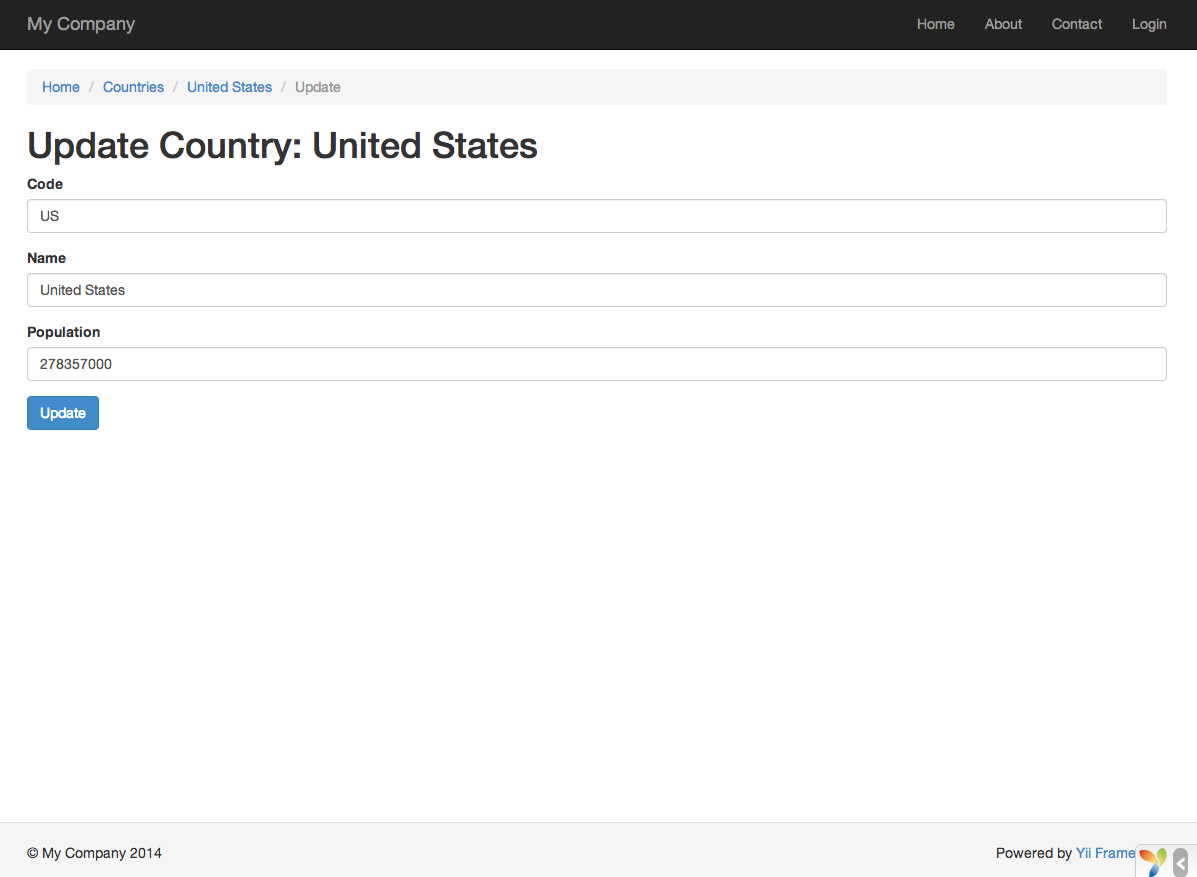
\includegraphics[width=\textwidth]{images/start-gii-country-update.png}

下面列出由 Gii 生成的文件,以便你研习功能和实现,或修改它们。

\begin{itemize}
\item 控制器:\lstinline|controllers/CountryController.php|
\item 模型:\lstinline|models/Country.php| 和 \lstinline|models/CountrySearch.php|
\item 视图:\lstinline|views/country/*.php|
\end{itemize}
\begin{quote}补充:Gii 被设计成高度可定制和可扩展的代码生成工具。使用它可以大幅提高应用开发速度。请参考 \hyperref[tool-gii.md]{Gii} 章节了解更多内容。

\end{quote}
\subsection{总结 \label{start-gii.md::summary}}
本章学习了如何使用 Gii 去生成为数据表中数据实现完整 CRUD 功能的代码。



\label{start-looking-ahead.md}\section{更上一层楼}
通篇阅读完整个“入门”部分,你就完成了一个完整 Yii 应用的创建。在此过程中你学到了如何实现一些常用功能,例如通过 HTML 表单从用户那获取数据,从数据库中获取数据并以分页形式显示。你还学到了如何通过 \hyperref[tool-gii.md]{Gii} 去自动生成代码。使用 Gii 生成代码把 Web 开发中多数繁杂的过程转化为仅仅填写几个表单就行。

本章将介绍一些有助于更好使用 Yii 的资源:

\begin{itemize}
\item 文档\begin{itemize}
\item 权威指南:顾名思义,指南详细描述了 Yii 的工作原理并提供了如何使用它的常规引导。这是最重要的 Yii 辅助资料,强烈建议在开始写 Yii 代码之前阅读。
\item 类参考手册:描述了 Yii 中每个类的用法。在编码过程中这极为有用,能够帮你理清某个特定类,方法,和属性的用法。类参考手册最好在整个框架的语境下去理解。
\item Wiki 文章:Wiki 文章是 Yii 用户在其自身经验基础上分享出来的。大多数是使用教程或如何使用 Yii 解决特定问题。虽然这些文章质量可能并不如权威指南,但它们往往覆盖了更广泛的话题,并常常提供解决方案,所以它们也很有用。
\item 书籍
\end{itemize}

\item 扩展\footnote{\url{http://www.yiiframework.com/extensions/}}:Yii 拥有数以千计用户提供的扩展,这些扩展能非常方便的插入到应用中,使你的应用开发过程更加方便快捷。
\item 社区\begin{itemize}
\item 官方论坛:\url{http://www.yiiframework.com/forum/}
\item IRC 聊天室:Freenode 网络上的 \#yii 频道 (\url{irc://irc.freenode.net/yii})(使用英文哦,无需反馈上游的问题可以加 
QQ-Yii2中国交流群)
\item GitHub:\url{https://github.com/yiisoft/yii2}
\item Facebook:\url{https://www.facebook.com/groups/yiitalk/}
\item Twitter:\url{https://twitter.com/yiiframework}
\item LinkedIn:\url{https://www.linkedin.com/groups/yii-framework-1483367}
\end{itemize}

\end{itemize}


\chapter{应用结构}
\label{structure-overview.md}\section{总览}
Yii 应用参照模型-视图-控制器 (MVC)\footnote{\url{http://wikipedia.org/wiki/Model-view-controller}}
 设计模式来组织。 \hyperref[structure-models.md]{模型}代表数据、业务逻辑和规则;\hyperref[structure-views.md]{视图}展示模型的输出;\hyperref[structure-controllers.md]{控制器}接受出入并将其转换为\hyperref[structure-models.md]{模型}和\hyperref[structure-views.md]{视图}命令。

除了 MVC, Yii 应用还有以下部分:

\begin{itemize}
\item \hyperref[structure-entry-scripts.md]{入口脚本}:终端用户能直接访问的 PHP 脚本,负责启动一个请求处理周期。
\item \hyperref[structure-applications.md]{应用}:能全局范围内访问的对象,管理协调组件来完成请求.
\item \hyperref[structure-application-components.md]{应用组件}:在应用中注册的对象,提供不同的功能来完成请求。
\item \hyperref[structure-modules.md]{模块}:包含完整 MVC 结构的独立包,一个应用可以由多个模块组建。 
\item \hyperref[structure-filters.md]{过滤器}:控制器在处理请求之前或之后需要触发执行的代码。
\item \hyperref[structure-widgets.md]{小部件}:可嵌入到\hyperref[structure-views.md]{视图}中的对象,可包含控制器逻辑,可被不同视图重复调用。
\end{itemize}
下面的示意图展示了 Yii 应用的静态结构:

\noindent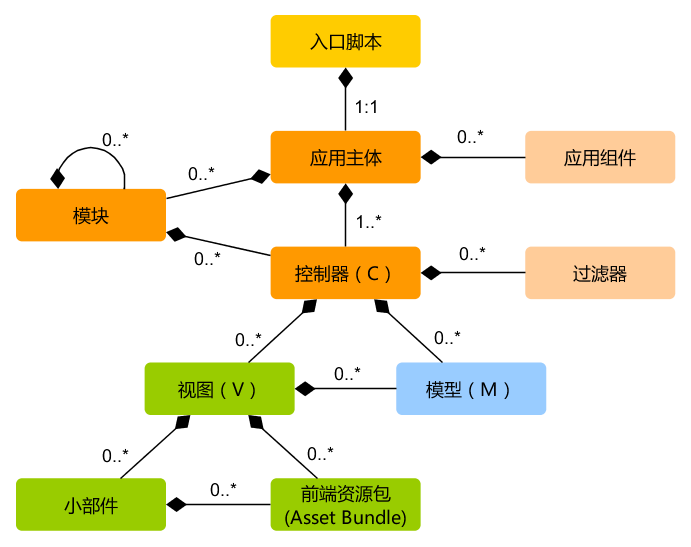
\includegraphics[width=\textwidth]{images/application-structure.png}



\label{structure-entry-scripts.md}\section{入口脚本}
入口脚本是应用启动流程中的第一环,一个应用(不管是网页应用还是控制台应用)只有一个入口脚本。终端用户的请求通过入口脚本实例化应用并将将请求转发到应用。

Web 应用的入口脚本必须放在终端用户能够访问的目录下,通常命名为 \lstinline|index.php|,也可以使用 Web 服务器能定位到的其他名称。

控制台应用的入口脚本一般在应用根目录下命名为 \lstinline|yii|(后缀为.php),该文件需要有执行权限,这样用户就能通过命令 \lstinline|./yii <route> [arguments] [options]| 来运行控制台应用。

入口脚本主要完成以下工作:

\begin{itemize}
\item 定义全局常量;
\item 注册 Composer 自动加载器\footnote{\url{http://getcomposer.org/doc/01-basic-usage.md\#autoloading}};
\item 包含 \texttt{Yii} 类文件;
\item 加载应用配置;
\item 创建一个\hyperref[structure-applications.md]{应用}实例并配置;
\item 调用 \texttt{yii{\allowbreak{}\textbackslash}base{\allowbreak{}\textbackslash}Application\allowbreak{}::\allowbreak{}run()} 来处理请求。
\end{itemize}
\subsection{Web 应用 \label{structure-entry-scripts.md::web-applications}}
以下是\hyperref[start-installation.md]{基础应用模版}入口脚本的代码:

\lstset{language=php}\begin{lstlisting}
<?php

defined('YII_DEBUG') or define('YII_DEBUG', true);
defined('YII_ENV') or define('YII_ENV', 'dev');

// 注册 Composer 自动加载器
require(__DIR__ . '/../vendor/autoload.php');

// 包含 Yii 类文件
require(__DIR__ . '/../vendor/yiisoft/yii2/Yii.php');

// 加载应用配置
$config = require(__DIR__ . '/../config/web.php');

// 创建、配置、运行一个应用
(new yii\web\Application($config))->run();
\end{lstlisting}
\subsection{控制台应用 \label{structure-entry-scripts.md::console-applications}}
以下是一个控制台应用的入口脚本:

\lstset{language=php}\begin{lstlisting}
#!/usr/bin/env php
<?php
/**
 * Yii console bootstrap file.
 *
 * @link http://www.yiiframework.com/
 * @copyright Copyright (c) 2008 Yii Software LLC
 * @license http://www.yiiframework.com/license/
 */

defined('YII_DEBUG') or define('YII_DEBUG', true);

// fcgi 默认没有定义 STDIN 和 STDOUT
defined('STDIN') or define('STDIN', fopen('php://stdin', 'r'));
defined('STDOUT') or define('STDOUT', fopen('php://stdout', 'w'));

// 注册 Composer 自动加载器
require(__DIR__ . '/vendor/autoload.php');

// 包含 Yii 类文件
require(__DIR__ . '/vendor/yiisoft/yii2/Yii.php');

// 加载应用配置
$config = require(__DIR__ . '/config/console.php');

$application = new yii\console\Application($config);
$exitCode = $application->run();
exit($exitCode);
\end{lstlisting}
\subsection{定义常量 \label{structure-entry-scripts.md::defining-constants}}
入口脚本是定义全局常量的最好地方,Yii 支持以下三个常量:

\begin{itemize}
\item \lstinline|YII_DEBUG|:标识应用是否运行在调试模式。当在调试模式下,应用会保留更多日志信息,如果抛出异常,会显示详细的错误调用堆栈。因此,调试模式主要适合在开发阶段使用,\lstinline|YII_DEBUG| 默认值为 false。
\item \lstinline|YII_ENV|:标识应用运行的环境,详情请查阅\hyperref[concept-configurations.md::environment-constants]{配置}章节。\lstinline|YII_ENV| 默认值为 \lstinline|'prod'|,表示应用运行在线上产品环境。
\item \lstinline|YII_ENABLE_ERROR_HANDLER|:标识是否启用 Yii 提供的错误处理,默认为 true。
\end{itemize}
当定义一个常量时,通常使用类似如下代码来定义:

\lstset{language=php}\begin{lstlisting}
defined('YII_DEBUG') or define('YII_DEBUG', true);
\end{lstlisting}
上面的代码等同于:

\lstset{language=php}\begin{lstlisting}
if (!defined('YII_DEBUG')) {
    define('YII_DEBUG', true);
}
\end{lstlisting}
显然第一段代码更加简洁易懂。

常量定义应该在入口脚本的开头,这样包含其他 PHP 文件时,常量就能生效。



\label{structure-applications.md}\section{应用主体}
应用主体是管理 Yii 应用系统整体结构和生命周期的对象。
每个Yii应用系统只能包含一个应用主体,应用主体在 \hyperref[structure-entry-scripts.md]{入口脚本} 中创建并能通过表达式 \lstinline|\Yii::$app| 全局范围内访问。

\begin{quote}补充: 当我们说''一个应用'',它可能是一个应用主体对象,也可能是一个应用系统,是根据上下文来决定[译:中文为避免歧义,Application翻译为应用主体]。

\end{quote}
Yii有两种应用主体: \texttt{yii{\allowbreak{}\textbackslash}web{\allowbreak{}\textbackslash}Application} and
\texttt{yii{\allowbreak{}\textbackslash}console{\allowbreak{}\textbackslash}Application}, 如名称所示,前者主要处理网页请求,后者处理控制台请求。

\subsection{应用主体配置 \label{structure-applications.md::application-configurations}}
如下所示,当 \hyperref[structure-entry-scripts.md]{入口脚本} 创建了一个应用主体,它会加载一个 \hyperref[concept-configurations.md]{配置} 文件并传给应用主体。

\lstset{language=php}\begin{lstlisting}
require(__DIR__ . '/../vendor/autoload.php');
require(__DIR__ . '/../vendor/yiisoft/yii2/Yii.php');

// 加载应用主体配置
$config = require(__DIR__ . '/../config/web.php');

// 实例化应用主体、配置应用主体
(new yii\web\Application($config))->run();
\end{lstlisting}
类似其他 \hyperref[concept-configurations.md]{配置} 文件, 应用主体配置文件标明如何设置应用对象初始属性。
由于应用主体配置比较复杂,一般保存在多个类似如上web.php的 \hyperref[concept-configurations.md::configuration-files]{配置文件} 当中。

\subsection{应用主体属性 \label{structure-applications.md::application-properties}}
应用主体配置文件中有许多重要的属性要配置,这些属性指定应用主体的运行环境。
比如,应用主体需要知道如何加载 \hyperref[structure-controllers.md]{控制器} ,临时文件保存到哪儿等等。
以下我们简述这些属性。

\subsubsection{必要属性 \label{structure-applications.md::required-properties}}
在一个应用中,至少要配置2个属性: \texttt{yii{\allowbreak{}\textbackslash}base{\allowbreak{}\textbackslash}Application\allowbreak{}::\allowbreak{}id} 和 \texttt{yii{\allowbreak{}\textbackslash}base{\allowbreak{}\textbackslash}Application\allowbreak{}::\allowbreak{}basePath}。

\paragraph{\texttt{yii{\allowbreak{}\textbackslash}base{\allowbreak{}\textbackslash}Application\allowbreak{}::\allowbreak{}id} \label{structure-applications.md::id}}
\texttt{yii{\allowbreak{}\textbackslash}base{\allowbreak{}\textbackslash}Application\allowbreak{}::\allowbreak{}id} 属性用来区分其他应用的唯一标识ID。主要给程序使用。
为了方便协作,最好使用数字作为应用主体ID,但不强制要求为数字。

\paragraph{\texttt{yii{\allowbreak{}\textbackslash}base{\allowbreak{}\textbackslash}Application\allowbreak{}::\allowbreak{}basePath} \label{structure-applications.md::basePath}}
\texttt{yii{\allowbreak{}\textbackslash}base{\allowbreak{}\textbackslash}Application\allowbreak{}::\allowbreak{}basePath} 指定该应用的根目录。根目录包含应用系统所有受保护的源代码。
在根目录下可以看到对应MVC设计模式的\lstinline|models|, \lstinline|views|, \lstinline|controllers|等子目录。

可以使用路径或 \hyperref[concept-aliases.md]{路径别名} 来在配置 \texttt{yii{\allowbreak{}\textbackslash}base{\allowbreak{}\textbackslash}Application\allowbreak{}::\allowbreak{}basePath} 属性。
两种格式所对应的目录都必须存在,否则系统会抛出一个异常。 系统会使用 \lstinline|realpath()| 函数规范化配置的路径.

\texttt{yii{\allowbreak{}\textbackslash}base{\allowbreak{}\textbackslash}Application\allowbreak{}::\allowbreak{}basePath} 属性经常用于派生一些其他重要路径(如runtime路径),因此,系统预定义 \lstinline|@app| 代表这个路径。
派生路径可以通过这个别名组成(如\lstinline|@app/runtime|代表runtime的路径)。

\subsubsection{重要属性 \label{structure-applications.md::important-properties}}
本小节所描述的属性通常需要设置,因为不用的应用属性不同。

\paragraph{\texttt{yii{\allowbreak{}\textbackslash}base{\allowbreak{}\textbackslash}Application\allowbreak{}::\allowbreak{}aliases} \label{structure-applications.md::aliases}}
该属性允许你用一个数组定义多个 \hyperref[concept-aliases.md]{别名}。数组的key为别名名称,值为对应的路径。例如:

\lstset{language=php}\begin{lstlisting}
[
    'aliases' => [
        '@name1' => 'path/to/path1',
        '@name2' => 'path/to/path2',
    ],
]
\end{lstlisting}
使用这个属性来定义别名,代替 \texttt{Yii\allowbreak{}::\allowbreak{}setAlias()} 方法来设置。

\paragraph{\texttt{yii{\allowbreak{}\textbackslash}base{\allowbreak{}\textbackslash}Application\allowbreak{}::\allowbreak{}bootstrap} \label{structure-applications.md::bootstrap}}
这个属性很实用,它允许你用数组指定启动阶段\texttt{yii{\allowbreak{}\textbackslash}base{\allowbreak{}\textbackslash}Application\allowbreak{}::\allowbreak{}bootstrap()}需要运行的组件。
比如,如果你希望一个 \hyperref[structure-modules.md]{模块} 自定义 \hyperref[runtime-url-handling.md]{URL 规则},你可以将模块ID加入到bootstrap数组中。

属性中的每个组件需要指定以下一项:

\begin{itemize}
\item 应用 \hyperref[structure-applications.md::::components]{组件} ID.
\item \hyperref[structure-applications.md::::modules]{模块} ID.
\item 类名.
\item 配置数组.
\item 创建并返回一个组件的无名称函数.
\end{itemize}
例如:

\lstset{language=php}\begin{lstlisting}
[
    'bootstrap' => [
        // 应用组件ID或模块ID
        'demo',

        // 类名
        'app\components\Profiler',

        // 配置数组
        [
            'class' => 'app\components\Profiler',
            'level' => 3,
        ],

        // 无名称函数
        function () {
            return new app\components\Profiler();
        }
    ],
]
\end{lstlisting}
\begin{quote}补充: 如果模块ID和应用组件ID同名,优先使用应用组件ID,如果你想用模块ID,可以使用如下无名称函数返回模块ID。
>\lstinline|`|php
[

\lstset{language={}}\begin{lstlisting}
function () {
    return Yii::$app->getModule('user');
},
\end{lstlisting}
]
\lstinline|`|

\end{quote}
在启动阶段,每个组件都会实例化。如果组件类实现接口 \texttt{yii{\allowbreak{}\textbackslash}base{\allowbreak{}\textbackslash}BootstrapInterface},也会调用 \texttt{yii{\allowbreak{}\textbackslash}base{\allowbreak{}\textbackslash}BootstrapInterface\allowbreak{}::\allowbreak{}bootstrap()} 方法。

举一个实际的例子,\hyperref[start-installation.md]{Basic Application Template} 应用主体配置中,
开发环境下会在启动阶段运行 \lstinline|debug| 和 \lstinline|gii| 模块。

\lstset{language=php}\begin{lstlisting}
if (YII_ENV_DEV) {
    // configuration adjustments for 'dev' environment
    $config['bootstrap'][] = 'debug';
    $config['modules']['debug'] = 'yii\debug\Module';

    $config['bootstrap'][] = 'gii';
    $config['modules']['gii'] = 'yii\gii\Module';
}
\end{lstlisting}
\begin{quote}注: 启动太多的组件会降低系统性能,因为每次请求都需要重新运行启动组件,因此谨慎配置启动组件。

\end{quote}
\paragraph{\texttt{yii{\allowbreak{}\textbackslash}web{\allowbreak{}\textbackslash}Application\allowbreak{}::\allowbreak{}catchAll} \label{structure-applications.md::catchAll}}
该属性仅 \texttt{yii{\allowbreak{}\textbackslash}web{\allowbreak{}\textbackslash}Application} 网页应用支持。
它指定一个要处理所有用户请求的 \hyperref[structure-controllers.md]{控制器方法},通常在维护模式下使用,同一个方法处理所有用户请求。

该配置为一个数组,第一项指定动作的路由,剩下的数组项(key-value 成对)指定传递给动作的参数,例如:

\lstset{language=php}\begin{lstlisting}
[
    'catchAll' => [
        'offline/notice',
        'param1' => 'value1',
        'param2' => 'value2',
    ],
]
\end{lstlisting}
\paragraph{\texttt{yii{\allowbreak{}\textbackslash}base{\allowbreak{}\textbackslash}Application\allowbreak{}::\allowbreak{}components} \label{structure-applications.md::components}}
这是最重要的属性,它允许你注册多个在其他地方使用的\hyperref[structure-applications.md::::structure-application-components.md]{应用组件}. 例如

\lstset{language=php}\begin{lstlisting}
[
    'components' => [
        'cache' => [
            'class' => 'yii\caching\FileCache',
        ],
        'user' => [
            'identityClass' => 'app\models\User',
            'enableAutoLogin' => true,
        ],
    ],
]
\end{lstlisting}
每一个应用组件指定一个key-value对的数组,key代表组件ID,value代表组件类名或 \hyperref[concept-configurations.md]{配置}。

在应用中可以任意注册组件,并可以通过表达式 \lstinline|\Yii::$app->ComponentID| 全局访问。

详情请阅读 \hyperref[structure-application-components.md]{应用组件} 一节.

\paragraph{\texttt{yii{\allowbreak{}\textbackslash}base{\allowbreak{}\textbackslash}Application\allowbreak{}::\allowbreak{}controllerMap} \label{structure-applications.md::controllerMap}}
该属性允许你指定一个控制器ID到任意控制器类。Yii遵循一个默认的 \hyperref[structure-applications.md::::controllerNamespace]{规则}指定控制器ID到任意控制器类(如\lstinline|post|对应\lstinline|app\controllers\PostController|)。
通过配置这个属性,可以打破这个默认规则,在下面的例子中,\lstinline|account|对应到\lstinline|app\controllers\UserController|,
\lstinline|article| 对应到 \lstinline|app\controllers\PostController|。

\lstset{language=php}\begin{lstlisting}
[
    'controllerMap' => [
        [
            'account' => 'app\controllers\UserController',
            'article' => [
                'class' => 'app\controllers\PostController',
                'enableCsrfValidation' => false,
            ],
        ],
    ],
]
\end{lstlisting}
数组的键代表控制器ID,数组的值代表对应的类名。

\paragraph{\texttt{yii{\allowbreak{}\textbackslash}base{\allowbreak{}\textbackslash}Application\allowbreak{}::\allowbreak{}controllerNamespace} \label{structure-applications.md::controllerNamespace}}
该属性指定控制器类默认的命名空间,默认为\lstinline|app\controllers|。比如控制器ID为 \lstinline|post| 默认对应 \lstinline|PostController| (不带命名空间),
类全名为 \lstinline|app\controllers\PostController|。

控制器类文件可能放在这个命名空间对应目录的子目录下,
例如,控制器ID \lstinline|admin/post| 对应的控制器类全名为 \lstinline|app\controllers\admin\PostController|。

控制器类全面能被 \hyperref[concept-autoloading.md]{自动加载},这点是非常重要的,控制器类的实际命名空间对应这个属性,
否则,访问时你会收到"Page Not Found''[译:页面找不到]。

如果你想打破上述的规则,可以配置 \hyperref[structure-applications.md::::controllerMap]{controllerMap} 属性。

\paragraph{\texttt{yii{\allowbreak{}\textbackslash}base{\allowbreak{}\textbackslash}Application\allowbreak{}::\allowbreak{}language} \label{structure-applications.md::language}}
该属性指定应用展示给终端用户的语言,默认为 \lstinline|en| 标识英文。如果需要之前其他语言可以配置该属性。

该属性影响各种 \hyperref[tutorial-i18n.md]{国际化} ,包括信息翻译、日期格式、数字格式等。
例如 \texttt{yii{\allowbreak{}\textbackslash}jui{\allowbreak{}\textbackslash}DatePicker} 小部件会根据该属性展示对应语言的日历以及日期格式。

推荐遵循 IETF language tag\footnote{\url{http://en.wikipedia.org/wiki/IETF\_language\_tag}} 来设置语言,例如 \lstinline|en| 代表英文, \lstinline|en-US| 代表英文(美国).

该属性的更多信息可参考 \hyperref[tutorial-i18n.md]{国际化} 一节.

\paragraph{\texttt{yii{\allowbreak{}\textbackslash}base{\allowbreak{}\textbackslash}Application\allowbreak{}::\allowbreak{}modules} \label{structure-applications.md::modules}}
该属性指定应用所包含的 \hyperref[structure-modules.md]{模块}。

该属性使用数组包含多个模块类 \hyperref[concept-configurations.md]{配置},数组的键为模块ID,例:

\lstset{language=php}\begin{lstlisting}
[
    'modules' => [
        // "booking" 模块以及对应的类
        'booking' => 'app\modules\booking\BookingModule',

        // "comment" 模块以及对应的配置数组
        'comment' => [
            'class' => 'app\modules\comment\CommentModule',
            'db' => 'db',
        ],
    ],
]
\end{lstlisting}
更多详情请参考 \hyperref[structure-modules.md]{模块} 一节。

\paragraph{\texttt{yii{\allowbreak{}\textbackslash}base{\allowbreak{}\textbackslash}Application\allowbreak{}::\allowbreak{}name} \label{structure-applications.md::name}}
该属性指定你可能想展示给终端用户的应用名称,不同于需要唯一性的 \texttt{yii{\allowbreak{}\textbackslash}base{\allowbreak{}\textbackslash}Application\allowbreak{}::\allowbreak{}id} 属性,
该属性可以不唯一,该属性用于显示应用的用途。

如果其他地方的代码没有用到,可以不配置该属性。

\paragraph{\texttt{yii{\allowbreak{}\textbackslash}base{\allowbreak{}\textbackslash}Application\allowbreak{}::\allowbreak{}params} \label{structure-applications.md::params}}
该属性为一个数组,指定可以全局访问的参数,代替程序中硬编码的数字和字符,应用中的参数定义到一个单独的文件并随时可以访问是一个好习惯。
例如用参数定义缩略图的长宽如下:

\lstset{language=php}\begin{lstlisting}
[
    'params' => [
        'thumbnail.size' => [128, 128],
    ],
]
\end{lstlisting}
然后简单的使用如下代码即可获取到你需要的长宽参数:

\lstset{language=php}\begin{lstlisting}
$size = \Yii::$app->params['thumbnail.size'];
$width = \Yii::$app->params['thumbnail.size'][0];
\end{lstlisting}
以后想修改缩略图长宽,只需要修改该参数而不需要相关的代码。

\paragraph{\texttt{yii{\allowbreak{}\textbackslash}base{\allowbreak{}\textbackslash}Application\allowbreak{}::\allowbreak{}sourceLanguage} \label{structure-applications.md::sourceLanguage}}
该属性指定应用代码的语言,默认为 \lstinline|'en-US'| 标识英文(美国),如果应用不是英文请修改该属性。

和 \hyperref[structure-applications.md::::language]{语言} 属性类似,配置该属性需遵循 IETF language tag\footnote{\url{http://en.wikipedia.org/wiki/IETF\_language\_tag}}.
例如 \lstinline|en| 代表英文, \lstinline|en-US| 代表英文(美国)。

该属性的更多信息可参考 \hyperref[tutorial-i18n.md]{国际化} 一节.

\paragraph{\texttt{yii{\allowbreak{}\textbackslash}base{\allowbreak{}\textbackslash}Application\allowbreak{}::\allowbreak{}timeZone} \label{structure-applications.md::timeZone}}
该属性提供一种方式修改PHP运行环境中的默认时区,配置该属性本质上就是调用PHP函数
date\_default\_timezone\_set()\footnote{\url{http://php.net/manual/en/function.date-default-timezone-set.php}},例如:

\lstset{language=php}\begin{lstlisting}
[
    'timeZone' => 'America/Los_Angeles',
]
\end{lstlisting}
\paragraph{\texttt{yii{\allowbreak{}\textbackslash}base{\allowbreak{}\textbackslash}Application\allowbreak{}::\allowbreak{}version} \label{structure-applications.md::version}}
该属性指定应用的版本,默认为\lstinline|'1.0'|,其他代码不使用的话可以不配置。

\subsubsection{实用属性 \label{structure-applications.md::useful-properties}}
本小节描述的属性不经常设置,通常使用系统默认值。如果你想改变默认值,可以配置这些属性。

\paragraph{\texttt{yii{\allowbreak{}\textbackslash}base{\allowbreak{}\textbackslash}Application\allowbreak{}::\allowbreak{}charset} \label{structure-applications.md::charset}}
该属性指定应用使用的字符集,默认值为 \lstinline|'UTF-8'|,绝大部分应用都在使用,除非已有的系统大量使用非unicode数据才需要更改该属性。

\paragraph{\texttt{yii{\allowbreak{}\textbackslash}base{\allowbreak{}\textbackslash}Application\allowbreak{}::\allowbreak{}defaultRoute} \label{structure-applications.md::defaultRoute}}
该属性指定未配置的请求的响应 \hyperref[runtime-routing.md]{路由} 规则,路由规则可能包含模块ID,控制器ID,动作ID。
例如\lstinline|help|, \lstinline|post/create|, \lstinline|admin/post/create|,如果动作ID没有指定,会使用\texttt{yii{\allowbreak{}\textbackslash}base{\allowbreak{}\textbackslash}Controller\allowbreak{}::\allowbreak{}defaultAction}中指定的默认值。

对于 \texttt{yii{\allowbreak{}\textbackslash}web{\allowbreak{}\textbackslash}Application} 网页应用,默认值为 \lstinline|'site'| 对应 \lstinline|SiteController| 控制器,并使用默认的动作。
因此你不带路由的访问应用,默认会显示 \lstinline|app\controllers\SiteController::actionIndex()| 的结果。

对于 \texttt{yii{\allowbreak{}\textbackslash}console{\allowbreak{}\textbackslash}Application} 控制台应用,
默认值为 \lstinline|'help'| 对应 \texttt{yii{\allowbreak{}\textbackslash}console{\allowbreak{}\textbackslash}controllers{\allowbreak{}\textbackslash}HelpController\allowbreak{}::\allowbreak{}actionIndex()}。
因此,如果执行的命令不带参数,默认会显示帮助信息。

\paragraph{\texttt{yii{\allowbreak{}\textbackslash}base{\allowbreak{}\textbackslash}Application\allowbreak{}::\allowbreak{}extensions} \label{structure-applications.md::extensions}}
该属性用数组列表指定应用安装和使用的 \hyperref[structure-extensions.md]{扩展},默认使用\lstinline|@vendor/yiisoft/extensions.php|文件返回的数组。
当你使用 Composer\footnote{\url{http://getcomposer.org}} 安装扩展,\lstinline|extensions.php| 会被自动生成和维护更新。
所以大多数情况下,不需要配置该属性。

特殊情况下你想自己手动维护扩展,可以参照如下配置该属性:

\lstset{language=php}\begin{lstlisting}
[
    'extensions' => [
        [
            'name' => 'extension name',
            'version' => 'version number',
            'bootstrap' => 'BootstrapClassName',  // 可选配,可为配置数组
            'alias' => [  // 可选配
                '@alias1' => 'to/path1',
                '@alias2' => 'to/path2',
            ],
        ],

        // ... 更多像上面的扩展 ...

    ],
]
\end{lstlisting}
如上所示,该属性包含一个扩展定义数组,每个扩展为一个包含 \lstinline|name| 和 \lstinline|version| 项的数组。
如果扩展要在 \hyperref[runtime-bootstrapping.md]{引导启动} 阶段运行,需要配置 \lstinline|bootstrap|以及对应的引导启动类名或 \hyperref[concept-configurations.md]{configuration} 数组。
扩展也可以定义 \hyperref[concept-aliases.md]{别名}

\paragraph{\texttt{yii{\allowbreak{}\textbackslash}base{\allowbreak{}\textbackslash}Application\allowbreak{}::\allowbreak{}layout} \label{structure-applications.md::layout}}
该属性指定渲染 \hyperref[structure-views.md]{视图} 默认使用的布局名字,默认值为 \lstinline|'main'| 对应\hyperref[structure-applications.md::::layoutPath]{布局路径}下的 \lstinline|main.php| 文件,
如果 \hyperref[structure-applications.md::::layoutPath]{布局路径} 和 \hyperref[structure-applications.md::::viewPath]{视图路径} 都是默认值,默认布局文件可以使用路径别名\lstinline|@app/views/layouts/main.php|

如果不想设置默认布局文件,可以设置该属性为 \lstinline|false|,这种做法比较罕见。

\paragraph{\texttt{yii{\allowbreak{}\textbackslash}base{\allowbreak{}\textbackslash}Application\allowbreak{}::\allowbreak{}layoutPath} \label{structure-applications.md::layoutPath}}
该属性指定查找布局文件的路径,默认值为 \hyperref[structure-applications.md::::viewPath]{视图路径} 下的 \lstinline|layouts| 子目录。
如果 \hyperref[structure-applications.md::::viewPath]{视图路径} 使用默认值,默认的布局路径别名为\lstinline|@app/views/layouts|。

该属性需要配置成一个目录或 路径 \hyperref[concept-aliases.md]{别名}。
You may configure it as a directory or a path \hyperref[concept-aliases.md]{alias}.

\paragraph{\texttt{yii{\allowbreak{}\textbackslash}base{\allowbreak{}\textbackslash}Application\allowbreak{}::\allowbreak{}runtimePath} \label{structure-applications.md::runtimePath}}
该属性指定临时文件如日志文件、缓存文件等保存路径,默认值为带别名的 \lstinline|@app/runtime|。

可以配置该属性为一个目录或者路径 \hyperref[concept-aliases.md]{别名},注意应用运行时有对该路径的写入权限,
以及终端用户不能访问改路径因为临时文件可能包含一些敏感信息。

为了简化访问该路径,Yii预定义别名 \lstinline|@runtime| 代表该路径。

\paragraph{\texttt{yii{\allowbreak{}\textbackslash}base{\allowbreak{}\textbackslash}Application\allowbreak{}::\allowbreak{}viewPath} \label{structure-applications.md::viewPath}}
该路径指定视图文件的根目录,默认值为带别名的 \lstinline|@app/views|,可以配置它为一个目录或者路径 \hyperref[concept-aliases.md]{别名}.

\paragraph{\texttt{yii{\allowbreak{}\textbackslash}base{\allowbreak{}\textbackslash}Application\allowbreak{}::\allowbreak{}vendorPath} \label{structure-applications.md::vendorPath}}
该属性指定 Composer\footnote{\url{http://getcomposer.org}} 管理的供应商路径,该路径包含应用使用的包括Yii框架在内的所有第三方库。
默认值为带别名的 \lstinline|@app/vendor| 。

可以配置它为一个目录或者路径 \hyperref[concept-aliases.md]{别名},当你修改时,务必修改对应的 Composer 配置。

为了简化访问该路径,Yii预定义别名 \lstinline|@vendor| 代表该路径。

\paragraph{\texttt{yii{\allowbreak{}\textbackslash}console{\allowbreak{}\textbackslash}Application\allowbreak{}::\allowbreak{}enableCoreCommands} \label{structure-applications.md::enableCoreCommands}}
该属性仅 \texttt{yii{\allowbreak{}\textbackslash}console{\allowbreak{}\textbackslash}Application} 控制台应用支持, 用来指定是否启用Yii中的核心命令,默认值为 \lstinline|true|。

\subsection{应用事件 \label{structure-applications.md::application-events}}
应用在处理请求过程中会触发事件,可以在配置文件配置事件处理代码,如下所示:

\lstset{language=php}\begin{lstlisting}
[
    'on beforeRequest' => function ($event) {
        // ...
    },
]
\end{lstlisting}
\lstinline|on eventName| 语法的用法在 \hyperref[concept-configurations.md::configuration-format]{Configurations} 一节有详细描述.

另外,在应用主体实例化后,你可以在\hyperref[runtime-bootstrapping.md]{引导启动} 阶段附加事件处理代码,例如:

\lstset{language=php}\begin{lstlisting}
\Yii::$app->on(\yii\base\Application::EVENT_BEFORE_REQUEST, function ($event) {
    // ...
});
\end{lstlisting}
\subsubsection{\texttt{yii{\allowbreak{}\textbackslash}base{\allowbreak{}\textbackslash}Application\allowbreak{}::\allowbreak{}EVENT\_BEFORE\_REQUEST} \label{structure-applications.md::beforeRequest}}
该事件在应用处理请求\textit{before}之前,实际的事件名为 \lstinline|beforeRequest|。

在事件触发前,应用主体已经实例化并配置好了,所以通过事件机制将你的代码嵌入到请求处理过程中非常不错。
例如在事件处理中根据某些参数动态设置\texttt{yii{\allowbreak{}\textbackslash}base{\allowbreak{}\textbackslash}Application\allowbreak{}::\allowbreak{}language}语言属性。

\subsubsection{\texttt{yii{\allowbreak{}\textbackslash}base{\allowbreak{}\textbackslash}Application\allowbreak{}::\allowbreak{}EVENT\_BEFORE\_REQUEST} \label{structure-applications.md::afterRequest}}
该事件在应用处理请求\textit{after}之后但在返回响应\textit{before}之前触发,实际的事件名为\lstinline|afterRequest|。

该事件触发时,请求已经被处理完,可以做一些请求后处理或自定义响应。

注意 \texttt{yii{\allowbreak{}\textbackslash}web{\allowbreak{}\textbackslash}Response} 组件在发送响应给终端用户时也会触发一些事件,这些事件都在本事件\textit{after}之后触发。

\subsubsection{\texttt{yii{\allowbreak{}\textbackslash}base{\allowbreak{}\textbackslash}Application\allowbreak{}::\allowbreak{}EVENT\_BEFORE\_REQUEST} \label{structure-applications.md::beforeAction}}
该事件在每个 \hyperref[structure-controllers.md]{控制器动作} 运行\textit{before}之前会被触发,实际的事件名为 \lstinline|beforeAction|.

事件的参数为一个 \texttt{yii{\allowbreak{}\textbackslash}base{\allowbreak{}\textbackslash}ActionEvent} 实例,
事件处理中可以设置\texttt{yii{\allowbreak{}\textbackslash}base{\allowbreak{}\textbackslash}ActionEvent\allowbreak{}::\allowbreak{}isValid} 为 \lstinline|false| 停止运行后续动作,例如:

\lstset{language=php}\begin{lstlisting}
[
    'on beforeAction' => function ($event) {
        if (some condition) {
            $event->isValid = false;
        } else {
        }
    },
]
\end{lstlisting}
注意 \hyperref[structure-modules.md]{模块} 和 \hyperref[structure-controllers.md]{控制器} 都会触发 \lstinline|beforeAction| 事件。
应用主体对象首先触发该事件,然后模块触发(如果存在模块),最后控制器触发。
任何一个事件处理中设置 \texttt{yii{\allowbreak{}\textbackslash}base{\allowbreak{}\textbackslash}ActionEvent\allowbreak{}::\allowbreak{}isValid} 设置为 \lstinline|false| 会停止触发后面的事件。

\subsubsection{\texttt{yii{\allowbreak{}\textbackslash}base{\allowbreak{}\textbackslash}Application\allowbreak{}::\allowbreak{}EVENT\_BEFORE\_REQUEST} \label{structure-applications.md::afterAction}}
该事件在每个 \hyperref[structure-controllers.md]{控制器动作} 运行\textit{after}之后会被触发,实际的事件名为 \lstinline|afterAction|.

该事件的参数为 \texttt{yii{\allowbreak{}\textbackslash}base{\allowbreak{}\textbackslash}ActionEvent} 实例,通过\texttt{yii{\allowbreak{}\textbackslash}base{\allowbreak{}\textbackslash}ActionEvent\allowbreak{}::\allowbreak{}result}属性,
事件处理可以访问和修改动作的结果。例如:

\lstset{language=php}\begin{lstlisting}
[
    'on afterAction' => function ($event) {
        if (some condition) {
            // 修改 $event->result
        } else {
        }
    },
]
\end{lstlisting}
注意 \hyperref[structure-modules.md]{模块} 和 \hyperref[structure-controllers.md]{控制器} 都会触发 \lstinline|afterAction| 事件。
这些对象的触发顺序和 \lstinline|beforeAction| 相反,也就是说,控制器最先触发,然后是模块(如果有模块),最后为应用主体。

\subsection{应用主体生命周期 \label{structure-applications.md::application-lifecycle}}
当运行 \hyperref[structure-entry-scripts.md]{入口脚本} 处理请求时,应用主体会经历以下生命周期:

\begin{enumerate}
\item 入口脚本加载应用主体配置数组。
\item 入口脚本创建一个应用主体实例:\begin{itemize}
\item 调用 \texttt{yii{\allowbreak{}\textbackslash}base{\allowbreak{}\textbackslash}Application\allowbreak{}::\allowbreak{}preInit()} 配置几个高级别应用主体属性,比如\texttt{yii{\allowbreak{}\textbackslash}base{\allowbreak{}\textbackslash}Application\allowbreak{}::\allowbreak{}basePath}。
\item 注册 \texttt{yii{\allowbreak{}\textbackslash}base{\allowbreak{}\textbackslash}Application\allowbreak{}::\allowbreak{}errorHandler} 错误处理方法.
\item 配置应用主体属性.
\item 调用 \texttt{yii{\allowbreak{}\textbackslash}base{\allowbreak{}\textbackslash}Application\allowbreak{}::\allowbreak{}init()} 初始化,该函数会调用 \texttt{yii{\allowbreak{}\textbackslash}base{\allowbreak{}\textbackslash}Application\allowbreak{}::\allowbreak{}bootstrap()} 运行引导启动组件.
\end{itemize}

\item 入口脚本调用 \texttt{yii{\allowbreak{}\textbackslash}base{\allowbreak{}\textbackslash}Application\allowbreak{}::\allowbreak{}run()} 运行应用主体:\begin{itemize}
\item 触发 \texttt{yii{\allowbreak{}\textbackslash}base{\allowbreak{}\textbackslash}Application\allowbreak{}::\allowbreak{}EVENT\_BEFORE\_REQUEST} 事件。
\item 处理请求:解析请求 \hyperref[runtime-routing.md]{路由} 和相关参数;创建路由指定的模块、控制器和动作对应的类,并运行动作。
\item 触发 \texttt{yii{\allowbreak{}\textbackslash}base{\allowbreak{}\textbackslash}Application\allowbreak{}::\allowbreak{}EVENT\_AFTER\_REQUEST} 事件。
\item 发送响应到终端用户.
\end{itemize}

\item 入口脚本接收应用主体传来的退出状态并完成请求的处理。
\end{enumerate}


\label{structure-application-components.md}\section{应用组件}
应用主体是\hyperref[concept-service-locator.md]{服务定位器},它部署一组提供各种不同功能的 \textit{应用组件} 来处理请求。
例如,\lstinline|urlManager|组件负责处理网页请求路由到对应的控制器。\lstinline|db|组件提供数据库相关服务等等。

在同一个应用中,每个应用组件都有一个独一无二的 ID 用来区分其他应用组件,你可以通过如下表达式访问应用组件。

\lstset{language=php}\begin{lstlisting}
\Yii::$app->componentID
\end{lstlisting}
例如,可以使用 \lstinline|\Yii::$app->db| 来获取到已注册到应用的 \texttt{yii{\allowbreak{}\textbackslash}db{\allowbreak{}\textbackslash}Connection},
使用 \lstinline|\Yii::$app->cache| 来获取到已注册到应用的 \texttt{yii{\allowbreak{}\textbackslash}caching{\allowbreak{}\textbackslash}Cache}。

第一次使用以上表达式时候会创建应用组件实例,后续再访问会返回此实例,无需再次创建。

应用组件可以是任意对象,可以在 \hyperref[structure-applications.md::application-configurations]{应用主体配置}配置 \texttt{yii{\allowbreak{}\textbackslash}base{\allowbreak{}\textbackslash}Application\allowbreak{}::\allowbreak{}components} 属性 .
例如:

\lstset{language=php}\begin{lstlisting}
[
    'components' => [
        // 使用类名注册 "cache" 组件
        'cache' => 'yii\caching\ApcCache',

        // 使用配置数组注册 "db" 组件
        'db' => [
            'class' => 'yii\db\Connection',
            'dsn' => 'mysql:host=localhost;dbname=demo',
            'username' => 'root',
            'password' => '',
        ],

        // 使用函数注册"search" 组件
        'search' => function () {
            return new app\components\SolrService;
        },
    ],
]
\end{lstlisting}
\begin{quote}补充:请谨慎注册太多应用组件,应用组件就像全局变量,使用太多可能加大测试和维护的难度。
  一般情况下可以在需要时再创建本地组件。

\end{quote}
\subsection{引导启动组件 \label{structure-application-components.md::bootstrapping-components}}
上面提到一个应用组件只会在第一次访问时实例化,如果处理请求过程没有访问的话就不实例化。
有时你想在每个请求处理过程都实例化某个组件即便它不会被访问,
可以将该组件ID加入到应用主体的 \texttt{yii{\allowbreak{}\textbackslash}base{\allowbreak{}\textbackslash}Application\allowbreak{}::\allowbreak{}bootstrap} 属性中。

例如, 如下的应用主体配置保证了 \lstinline|log| 组件一直被加载。

\lstset{language=php}\begin{lstlisting}
[
    'bootstrap' => [
        // 将 log 组件 ID 加入引导让它始终载入
        'log',
    ],
    'components' => [
        'log' => [
            // "log" 组件的配置
        ],
    ],
]
\end{lstlisting}
\subsection{核心应用组件 \label{structure-application-components.md::core-application-components}}
Yii 定义了一组固定ID和默认配置的 \textit{核心} 组件,例如 \texttt{yii{\allowbreak{}\textbackslash}web{\allowbreak{}\textbackslash}Application\allowbreak{}::\allowbreak{}request} 组件
用来收集用户请求并解析 \hyperref[runtime-routing.md]{路由};
\texttt{yii{\allowbreak{}\textbackslash}base{\allowbreak{}\textbackslash}Application\allowbreak{}::\allowbreak{}db} 代表一个可以执行数据库操作的数据库连接。
通过这些组件,Yii应用主体能处理用户请求。

下面是预定义的核心应用组件列表,可以和普通应用组件一样配置和自定义它们。
当你配置一个核心组件,不指定它的类名的话就会使用Yii默认指定的类。

\begin{itemize}
\item \texttt{yii{\allowbreak{}\textbackslash}web{\allowbreak{}\textbackslash}AssetManager}: 管理资源包和资源发布,详情请参考 \hyperref[output-assets.md]{管理资源} 一节。
\item 注意配置该组件时必须指定组件类名和其他相关组件属性,如\texttt{yii{\allowbreak{}\textbackslash}db{\allowbreak{}\textbackslash}Connection\allowbreak{}::\allowbreak{}dsn}。
详情请参考 \hyperref[db-dao.md]{数据访问对象} 一节。


\item \texttt{yii{\allowbreak{}\textbackslash}base{\allowbreak{}\textbackslash}Application\allowbreak{}::\allowbreak{}errorHandler}: 处理 PHP 错误和异常,
详情请参考 \hyperref[tutorial-handling-errors.md]{错误处理} 一节。
\item 日期使用长格式。详情请参考 \hyperref[output-formatting.md]{格式化输出数据} 一节。


\item \texttt{yii{\allowbreak{}\textbackslash}i18n{\allowbreak{}\textbackslash}I18N}: 支持信息翻译和格式化。详情请参考 \hyperref[tutorial-i18n.md]{国际化} 一节。
\item \texttt{yii{\allowbreak{}\textbackslash}log{\allowbreak{}\textbackslash}Dispatcher}: 管理日志对象。详情请参考 \hyperref[tutorial-logging.md]{日志} 一节。
\item \texttt{yii{\allowbreak{}\textbackslash}swiftmailer{\allowbreak{}\textbackslash}Mailer}: 支持生成邮件结构并发送,详情请参考 \hyperref[tutorial-mailing.md]{邮件} 一节。
\item 详情请参考 \hyperref[runtime-responses.md]{响应} 一节。


\item 详情请参考 \hyperref[runtime-requests.md]{请求} 一节。


\item \texttt{yii{\allowbreak{}\textbackslash}web{\allowbreak{}\textbackslash}Session}: 代表会话信息,仅在\texttt{yii{\allowbreak{}\textbackslash}web{\allowbreak{}\textbackslash}Application} 网页应用中可用,
详情请参考 \hyperref[runtime-sessions-cookies.md]{Sessions (会话) and Cookies} 一节。
\item 详情请参考 \hyperref[runtime-url-handling.md]{URL 解析和生成} 一节。


\item \texttt{yii{\allowbreak{}\textbackslash}web{\allowbreak{}\textbackslash}User}: 代表认证登录用户信息,仅在\texttt{yii{\allowbreak{}\textbackslash}web{\allowbreak{}\textbackslash}Application} 网页应用中可用,
详情请参考 \hyperref[security-authentication.md]{认证} 一节。
\item \texttt{yii{\allowbreak{}\textbackslash}web{\allowbreak{}\textbackslash}View}: 支持渲染视图,详情请参考 \hyperref[structure-views.md]{Views} 一节。
\end{itemize}


\label{structure-controllers.md}\section{控制器}
控制器是 MVC\footnote{\url{http://en.wikipedia.org/wiki/Model\%E2\%80\%93view\%E2\%80\%93controller}} 模式中的一部分,
是继承\texttt{yii{\allowbreak{}\textbackslash}base{\allowbreak{}\textbackslash}Controller}类的对象,负责处理请求和生成响应。
具体来说,控制器从\hyperref[structure-applications.md]{应用主体}接管控制后会分析请求数据并传送到\hyperref[structure-models.md]{模型},
传送模型结果到\hyperref[structure-views.md]{视图},最后生成输出响应信息。

\subsection{操作 \label{structure-controllers.md::actions}}
控制器由 \textit{操作} 组成,它是执行终端用户请求的最基础的单元,一个控制器可有一个或多个操作。

如下示例显示包含两个操作\lstinline|view| and \lstinline|create| 的控制器\lstinline|post|:

\lstset{language=php}\begin{lstlisting}
namespace app\controllers;

use Yii;
use app\models\Post;
use yii\web\Controller;
use yii\web\NotFoundHttpException;

class PostController extends Controller
{
    public function actionView($id)
    {
        $model = Post::findOne($id);
        if ($model === null) {
            throw new NotFoundHttpException;
        }

        return $this->render('view', [
            'model' => $model,
        ]);
    }

    public function actionCreate()
    {
        $model = new Post;

        if ($model->load(Yii::$app->request->post()) && $model->save()) {
            return $this->redirect(['view', 'id' => $model->id]);
        } else {
            return $this->render('create', [
                'model' => $model,
            ]);
        }
    }
}
\end{lstlisting}
在操作 \lstinline|view| (定义为 \lstinline|actionView()| 方法)中, 代码首先根据请求模型ID加载 \hyperref[structure-models.md]{模型},
如果加载成功,会渲染名称为\lstinline|view|的\hyperref[structure-views.md]{视图}并显示,否则会抛出一个异常。

在操作 \lstinline|create| (定义为 \lstinline|actionCreate()| 方法)中, 代码相似. 先将请求数据填入\hyperref[structure-models.md]{模型},
然后保存模型,如果两者都成功,会跳转到ID为新创建的模型的\lstinline|view|操作,否则显示提供用户输入的\lstinline|create|视图。

\subsection{路由 \label{structure-controllers.md::routes}}
终端用户通过所谓的\textit{路由}寻找到操作,路由是包含以下部分的字符串:

\begin{itemize}
\item 模型ID: 仅存在于控制器属于非应用的\hyperref[structure-modules.md]{模块};
\item 控制器ID: 同应用(或同模块如果为模块下的控制器)下唯一标识控制器的字符串;
\item 操作ID: 同控制器下唯一标识操作的字符串。
\end{itemize}
路由使用如下格式:

\lstset{language={}}\begin{lstlisting}
ControllerID/ActionID
\end{lstlisting}
如果属于模块下的控制器,使用如下格式:

\lstset{language=php}\begin{lstlisting}
ModuleID/ControllerID/ActionID
\end{lstlisting}
如果用户的请求地址为 \lstinline|http://hostname/index.php?r=site/index|, 会执行\lstinline|site| 控制器的\lstinline|index| 操作。
更多关于处理路由的详情请参阅 \hyperref[runtime-routing.md]{路由} 一节。

\subsection{创建控制器 \label{structure-controllers.md::creating-controllers}}
在\texttt{yii{\allowbreak{}\textbackslash}web{\allowbreak{}\textbackslash}Application}网页应用中,控制器应继承\texttt{yii{\allowbreak{}\textbackslash}web{\allowbreak{}\textbackslash}Controller} 或它的子类。
同理在\texttt{yii{\allowbreak{}\textbackslash}console{\allowbreak{}\textbackslash}Application}控制台应用中,控制器继承\texttt{yii{\allowbreak{}\textbackslash}console{\allowbreak{}\textbackslash}Controller} 或它的子类。
如下代码定义一个 \lstinline|site| 控制器:

\lstset{language=php}\begin{lstlisting}
namespace app\controllers;

use yii\web\Controller;

class SiteController extends Controller
{
}
\end{lstlisting}
\subsubsection{控制器ID \label{structure-controllers.md::controller-ids}}
通常情况下,控制器用来处理请求有关的资源类型,因此控制器ID通常为和资源有关的名词。
例如使用\lstinline|article|作为处理文章的控制器ID。

控制器ID应仅包含英文小写字母、数字、下划线、中横杠和正斜杠,
例如 \lstinline|article| 和 \lstinline|post-comment| 是真是的控制器ID,\lstinline|article?|, \lstinline|PostComment|, \lstinline|admin\post|不是控制器ID。

控制器Id可包含子目录前缀,例如 \lstinline|admin/article| 代表
\texttt{yii{\allowbreak{}\textbackslash}base{\allowbreak{}\textbackslash}Application\allowbreak{}::\allowbreak{}controllerNamespace}控制器命名空间下 \lstinline|admin|子目录中 \lstinline|article| 控制器。
子目录前缀可为英文大小写字母、数字、下划线、正斜杠,其中正斜杠用来区分多级子目录(如 \lstinline|panels/admin|)。

\subsubsection{控制器类命名 \label{structure-controllers.md::controller-class-naming}}
控制器ID遵循以下规则衍生控制器类名:

\begin{itemize}
\item 将用正斜杠区分的每个单词第一个字母转为大写。注意如果控制器ID包含正斜杠,只将最后的正斜杠后的部分第一个字母转为大写;
\item 去掉中横杠,将正斜杠替换为反斜杠;
\item 增加\lstinline|Controller|后缀;
\item 在前面增加\texttt{yii{\allowbreak{}\textbackslash}base{\allowbreak{}\textbackslash}Application\allowbreak{}::\allowbreak{}controllerNamespace}控制器命名空间.
\end{itemize}
下面为一些示例,假设\texttt{yii{\allowbreak{}\textbackslash}base{\allowbreak{}\textbackslash}Application\allowbreak{}::\allowbreak{}controllerNamespace}控制器命名空间为 \lstinline|app\controllers|:

\begin{itemize}
\item \lstinline|article| 对应 \lstinline|app\controllers\ArticleController|;
\item \lstinline|post-comment| 对应 \lstinline|app\controllers\PostCommentController|;
\item \lstinline|admin/post-comment| 对应 \lstinline|app\controllers\admin\PostCommentController|;
\item \lstinline|adminPanels/post-comment| 对应 \lstinline|app\controllers\adminPanels\PostCommentController|.
\end{itemize}
控制器类必须能被 \hyperref[concept-autoloading.md]{自动加载},所以在上面的例子中,
控制器\lstinline|article| 类应在 \hyperref[concept-aliases.md]{别名} 为\lstinline|@app/controllers/ArticleController.php|的文件中定义,
控制器\lstinline|admin/post2-comment|应在\lstinline|@app/controllers/admin/Post2CommentController.php|文件中。

\begin{quote}补充: 最后一个示例 \lstinline|admin/post2-comment| 表示你可以将控制器放在
  \texttt{yii{\allowbreak{}\textbackslash}base{\allowbreak{}\textbackslash}Application\allowbreak{}::\allowbreak{}controllerNamespace}控制器命名空间下的子目录中,
  在你不想用 \hyperref[structure-modules.md]{模块} 的情况下给控制器分类,这种方式很有用。

\end{quote}
\subsubsection{控制器部署 \label{structure-controllers.md::controller-map}}
可通过配置 \texttt{yii{\allowbreak{}\textbackslash}base{\allowbreak{}\textbackslash}Application\allowbreak{}::\allowbreak{}controllerMap} 来强制上述的控制器ID和类名对应,
通常用在使用第三方不能掌控类名的控制器上。

配置 \hyperref[structure-applications.md::application-configurations]{应用配置} 
中的\hyperref[structure-applications.md::application-configurations]{application configuration},如下所示:

\lstset{language=php}\begin{lstlisting}
[
    'controllerMap' => [
        // 用类名申明 "account" 控制器
        'account' => 'app\controllers\UserController',

        // 用配置数组申明 "article" 控制器
        'article' => [
            'class' => 'app\controllers\PostController',
            'enableCsrfValidation' => false,
        ],
    ],
]
\end{lstlisting}
\subsubsection{默认控制器 \label{structure-controllers.md::default-controller}}
每个应用有一个由\texttt{yii{\allowbreak{}\textbackslash}base{\allowbreak{}\textbackslash}Application\allowbreak{}::\allowbreak{}defaultRoute}属性指定的默认控制器;
当请求没有指定 \hyperref[structure-controllers.md::::ids-routes]{路由},该属性值作为路由使用。
对于\texttt{yii{\allowbreak{}\textbackslash}web{\allowbreak{}\textbackslash}Application}网页应用,它的值为 \lstinline|'site'|,
对于 \texttt{yii{\allowbreak{}\textbackslash}console{\allowbreak{}\textbackslash}Application}控制台应用,它的值为 \lstinline|help|,
所以URL为 \lstinline|http://hostname/index.php| 表示由 \lstinline|site| 控制器来处理。

可以在 \hyperref[structure-applications.md::application-configurations]{应用配置} 中修改默认控制器,如下所示:

\lstset{language=php}\begin{lstlisting}
[
    'defaultRoute' => 'main',
]
\end{lstlisting}
\subsection{创建操作 \label{structure-controllers.md::creating-actions}}
创建操作可简单地在控制器类中定义所谓的 \textit{操作方法} 来完成,操作方法必须是以\lstinline|action|开头的公有方法。
操作方法的返回值会作为响应数据发送给终端用户,如下代码定义了两个操作 \lstinline|index| 和 \lstinline|hello-world|:

\lstset{language=php}\begin{lstlisting}
namespace app\controllers;

use yii\web\Controller;

class SiteController extends Controller
{
    public function actionIndex()
    {
        return $this->render('index');
    }

    public function actionHelloWorld()
    {
        return 'Hello World';
    }
}
\end{lstlisting}
\subsubsection{操作ID \label{structure-controllers.md::action-ids}}
操作通常是用来执行资源的特定操作,因此,操作ID通常为动词,如\lstinline|view|, \lstinline|update|等。

操作ID应仅包含英文小写字母、数字、下划线和中横杠,操作ID中的中横杠用来分隔单词。
例如\lstinline|view|, \lstinline|update2|, \lstinline|comment-post|是真实的操作ID,\lstinline|view?|, \lstinline|Update|不是操作ID.

可通过两种方式创建操作ID,内联操作和独立操作. An inline action is
内联操作在控制器类中定义为方法;独立操作是继承\texttt{yii{\allowbreak{}\textbackslash}base{\allowbreak{}\textbackslash}Action}或它的子类的类。
内联操作容易创建,在无需重用的情况下优先使用;
独立操作相反,主要用于多个控制器重用,或重构为\hyperref[structure-extensions.md]{扩展}。

\subsubsection{内联操作 \label{structure-controllers.md::inline-actions}}
内联操作指的是根据我们刚描述的操作方法。

操作方法的名字是根据操作ID遵循如下规则衍生:

\begin{itemize}
\item 将每个单词的第一个字母转为大写;
\item 去掉中横杠;
\item 增加\lstinline|action|前缀.
\end{itemize}
例如\lstinline|index| 转成 \lstinline|actionIndex|, \lstinline|hello-world| 转成 \lstinline|actionHelloWorld|。

\begin{quote}注意: 操作方法的名字\textit{大小写敏感},如果方法名称为\lstinline|ActionIndex|不会认为是操作方法,
  所以请求\lstinline|index|操作会返回一个异常,也要注意操作方法必须是公有的,私有或者受保护的方法不能定义成内联操作。

\end{quote}
因为容易创建,内联操作是最常用的操作,但是如果你计划在不同地方重用相同的操作,
或者你想重新分配一个操作,需要考虑定义它为\textit{独立操作}。

\subsubsection{独立操作 \label{structure-controllers.md::standalone-actions}}
独立操作通过继承\texttt{yii{\allowbreak{}\textbackslash}base{\allowbreak{}\textbackslash}Action}或它的子类来定义。
例如Yii发布的\texttt{yii{\allowbreak{}\textbackslash}web{\allowbreak{}\textbackslash}ViewAction}和\texttt{yii{\allowbreak{}\textbackslash}web{\allowbreak{}\textbackslash}ErrorAction}都是独立操作。

要使用独立操作,需要通过控制器中覆盖\texttt{yii{\allowbreak{}\textbackslash}base{\allowbreak{}\textbackslash}Controller\allowbreak{}::\allowbreak{}actions()}方法在\textit{action map}中申明,如下例所示:

\lstset{language=php}\begin{lstlisting}
public function actions()
{
    return [
        // 用类来申明"error" 操作
        'error' => 'yii\web\ErrorAction',

        // 用配置数组申明 "view" 操作
        'view' => [
            'class' => 'yii\web\ViewAction',
            'viewPrefix' => '',
        ],
    ];
}
\end{lstlisting}
如上所示, \lstinline|actions()| 方法返回键为操作ID、值为对应操作类名或数组\hyperref[concept-configurations.md]{configurations} 的数组。
和内联操作不同,独立操作ID可包含任意字符,只要在\lstinline|actions()| 方法中申明.

为创建一个独立操作类,需要继承\texttt{yii{\allowbreak{}\textbackslash}base{\allowbreak{}\textbackslash}Action} 或它的子类,并实现公有的名称为\lstinline|run()|的方法,
\lstinline|run()| 方法的角色和操作方法类似,例如:

\lstset{language=php}\begin{lstlisting}
<?php
namespace app\components;

use yii\base\Action;

class HelloWorldAction extends Action
{
    public function run()
    {
        return "Hello World";
    }
}
\end{lstlisting}
\subsubsection{操作结果 \label{structure-controllers.md::action-results}}
操作方法或独立操作的\lstinline|run()|方法的返回值非常中药,它表示对应操作结果。

返回值可为 \hyperref[runtime-responses.md]{响应} 对象,作为响应发送给终端用户。

\begin{itemize}
\item 对于\texttt{yii{\allowbreak{}\textbackslash}web{\allowbreak{}\textbackslash}Application}网页应用,返回值可为任意数据, 它赋值给\texttt{yii{\allowbreak{}\textbackslash}web{\allowbreak{}\textbackslash}Response\allowbreak{}::\allowbreak{}data},
最终转换为字符串来展示响应内容。
\item 对于\texttt{yii{\allowbreak{}\textbackslash}console{\allowbreak{}\textbackslash}Application}控制台应用,返回值可为整数,
表示命令行下执行的 \texttt{yii{\allowbreak{}\textbackslash}console{\allowbreak{}\textbackslash}Response\allowbreak{}::\allowbreak{}exitStatus} 退出状态。
\end{itemize}
在上面的例子中,操作结果都为字符串,作为响应数据发送给终端用户,下例显示一个操作通过
返回响应对象(因为\texttt{yii{\allowbreak{}\textbackslash}web{\allowbreak{}\textbackslash}Controller\allowbreak{}::\allowbreak{}redirect()}方法返回一个响应对象)可将用户浏览器跳转到新的URL。

\lstset{language=php}\begin{lstlisting}
public function actionForward()
{
    // 用户浏览器跳转到 http://example.com
    return $this->redirect('http://example.com');
}
\end{lstlisting}
\subsubsection{操作参数 \label{structure-controllers.md::action-parameters}}
内联操作的操作方法和独立操作的 \lstinline|run()| 方法可以带参数,称为\textit{操作参数}。
参数值从请求中获取,对于\texttt{yii{\allowbreak{}\textbackslash}web{\allowbreak{}\textbackslash}Application}网页应用,
每个操作参数的值从\lstinline|$_GET|中获得,参数名作为键;
对于\texttt{yii{\allowbreak{}\textbackslash}console{\allowbreak{}\textbackslash}Application}控制台应用, 操作参数对应命令行参数。

如下例,操作\lstinline|view| (内联操作) 申明了两个参数 \lstinline|$id| 和 \lstinline|$version|。

\lstset{language=php}\begin{lstlisting}
namespace app\controllers;

use yii\web\Controller;

class PostController extends Controller
{
    public function actionView($id, $version = null)
    {
        // ...
    }
}
\end{lstlisting}
操作参数会被不同的参数填入,如下所示:

\begin{itemize}
\item \lstinline|http://hostname/index.php?r=post/view&id=123|: \lstinline|$id| 会填入\lstinline|'123'|,\lstinline|$version| 仍为 null 空因为没有\lstinline|version|请求参数;
\item \lstinline|http://hostname/index.php?r=post/view&id=123&version=2|: \$id\lstinline| 和 |\$version\lstinline| 分别填入 |`123'\lstinline| 和 |`2'`;
\item \lstinline|http://hostname/index.php?r=post/view|: 会抛出\texttt{yii{\allowbreak{}\textbackslash}web{\allowbreak{}\textbackslash}BadRequestHttpException} 异常
因为请求没有提供参数给必须赋值参数\lstinline|$id|;
\item \lstinline|http://hostname/index.php?r=post/view&id[]=123|: 会抛出\texttt{yii{\allowbreak{}\textbackslash}web{\allowbreak{}\textbackslash}BadRequestHttpException} 异常
因为\lstinline|$id| 参数收到数字值 \lstinline|['123']|而不是字符串.
\end{itemize}
如果想让操作参数接收数组值,需要指定\$id为\lstinline|array|,如下所示:

\lstset{language=php}\begin{lstlisting}
public function actionView(array $id, $version = null)
{
    // ...
}
\end{lstlisting}
现在如果请求为 \lstinline|http://hostname/index.php?r=post/view&id[]=123|, 参数 \lstinline|$id| 会使用数组值\lstinline|['123']|,
如果请求为 \lstinline|http://hostname/index.php?r=post/view&id=123|,
参数 \lstinline|$id| 会获取相同数组值,因为无类型的\lstinline|'123'|会自动转成数组。

上述例子主要描述网页应用的操作参数,对于控制台应用,更多详情请参阅\hyperref[tutorial-console.md]{控制台命令}。

\subsubsection{默认操作 \label{structure-controllers.md::default-action}}
每个控制器都有一个由 \texttt{yii{\allowbreak{}\textbackslash}base{\allowbreak{}\textbackslash}Controller\allowbreak{}::\allowbreak{}defaultAction} 属性指定的默认操作,
当\hyperref[structure-controllers.md::::ids-routes]{路由} 只包含控制器ID,会使用所请求的控制器的默认操作。

默认操作默认为 \lstinline|index|,如果想修改默认操作,只需简单地在控制器类中覆盖这个属性,如下所示:

\lstset{language=php}\begin{lstlisting}
namespace app\controllers;

use yii\web\Controller;

class SiteController extends Controller
{
    public $defaultAction = 'home';

    public function actionHome()
    {
        return $this->render('home');
    }
}
\end{lstlisting}
\subsection{控制器生命周期 \label{structure-controllers.md::controller-lifecycle}}
处理一个请求时,\hyperref[structure-applications.md]{应用主体} 会根据请求\hyperref[structure-controllers.md::::routes]{路由}创建一个控制器,will create a controller
控制器经过以下生命周期来完成请求:

\begin{enumerate}
\item 在控制器创建和配置后,\texttt{yii{\allowbreak{}\textbackslash}base{\allowbreak{}\textbackslash}Controller\allowbreak{}::\allowbreak{}init()} 方法会被调用。
\item 控制器根据请求操作ID创建一个操作对象:\begin{itemize}
\item 如果操作ID没有指定,会使用\texttt{yii{\allowbreak{}\textbackslash}base{\allowbreak{}\textbackslash}Controller\allowbreak{}::\allowbreak{}defaultAction}默认操作ID;
\item 如果在\texttt{yii{\allowbreak{}\textbackslash}base{\allowbreak{}\textbackslash}Controller\allowbreak{}::\allowbreak{}actions()}找到操作ID,会创建一个独立操作;
\item 如果操作ID对应操作方法,会创建一个内联操作;
\item 否则会抛出\texttt{yii{\allowbreak{}\textbackslash}base{\allowbreak{}\textbackslash}InvalidRouteException}异常。
\end{itemize}

\item 控制器按顺序调用应用主体、模块(如果控制器属于模块)、控制器的 \lstinline|beforeAction()| 方法;\begin{itemize}
\item 如果任意一个调用返回false,后面未调用的\lstinline|beforeAction()|会跳过并且操作执行会被取消;
action execution will be cancelled.
\item 默认情况下每个 \lstinline|beforeAction()| 方法会触发一个 \lstinline|beforeAction| 事件,在事件中你可以追加事件处理操作;
\end{itemize}

\item 控制器执行操作:\begin{itemize}
\item 请求数据解析和填入到操作参数;
\end{itemize}

\item 控制器按顺序调用控制器、模块(如果控制器属于模块)、应用主体的 \lstinline|afterAction()| 方法;\begin{itemize}
\item 默认情况下每个 \lstinline|afterAction()| 方法会触发一个 \lstinline|afterAction| 事件,在事件中你可以追加事件处理操作;
\end{itemize}

\item 应用主体获取操作结果并赋值给\hyperref[runtime-responses.md]{响应}.
\end{enumerate}
\subsection{最佳实践 \label{structure-controllers.md::best-practices}}
在设计良好的应用中,控制器很精练,包含的操作代码简短;
如果你的控制器很复杂,通常意味着需要重构,转移一些代码到其他类中。

归纳起来,控制器

\begin{itemize}
\item 可访问 \hyperref[runtime-requests.md]{请求} 数据;
\item 可根据请求数据调用 \hyperref[structure-models.md]{模型} 的方法和其他服务组件;
\item 可使用 \hyperref[structure-views.md]{视图} 构造响应;
\item 不应处理应被\hyperref[structure-models.md]{模型}处理的请求数据;
\item 应避免嵌入HTML或其他展示代码,这些代码最好在 \hyperref[structure-views.md]{视图}中处理.
\end{itemize}


\label{structure-views.md}\section{视图}
视图是 MVC\footnote{\url{http://en.wikipedia.org/wiki/Model\%E2\%80\%93view\%E2\%80\%93controller}} 模式中的一部分。
它是展示数据到终端用户的代码,在网页应用中,根据\textit{视图模板}来创建视图,视图模板为PHP脚本文件,
主要包含HTML代码和展示类PHP代码,通过\texttt{yii{\allowbreak{}\textbackslash}web{\allowbreak{}\textbackslash}View}应用组件来管理,
该组件主要提供通用方法帮助视图构造和渲染,简单起见,我们称视图模板或视图模板文件为视图。

\subsection{创建视图 \label{structure-views.md::creating-views}}
如前所述,视图为包含HTML和PHP代码的PHP脚本,如下代码为一个登录表单的视图,
可看到PHP代码用来生成动态内容如页面标题和表单,HTML代码把它组织成一个漂亮的HTML页面。

\lstset{language=php}\begin{lstlisting}
<?php
use yii\helpers\Html;
use yii\widgets\ActiveForm;

/* @var $this yii\web\View */
/* @var $form yii\widgets\ActiveForm */
/* @var $model app\models\LoginForm */

$this->title = 'Login';
?>
<h1><?= Html::encode($this->title) ?></h1>

<p>Please fill out the following fields to login:</p>

<?php $form = ActiveForm::begin(); ?>
    <?= $form->field($model, 'username') ?>
    <?= $form->field($model, 'password')->passwordInput() ?>
    <?= Html::submitButton('Login') ?>
<?php ActiveForm::end(); ?>
\end{lstlisting}
在视图中,可访问 \lstinline|$this| 指向 \texttt{yii{\allowbreak{}\textbackslash}web{\allowbreak{}\textbackslash}View} 来管理和渲染这个视图文件。

除了 \lstinline|$this|之外,上述示例中的视图有其他预定义变量如 \lstinline|$model|,
这些变量代表从\hyperref[structure-controllers.md]{控制器}或其他触发\hyperref[structure-views.md::::rendering-views]{视图渲染}的对象 \textit{传入} 到视图的数据。

\begin{quote}技巧: 将预定义变量列到视图文件头部注释处,这样可被IDE编辑器识别,也是生成视图文档的好方法。

\end{quote}
\subsubsection{安全 \label{structure-views.md::security}}
当创建生成HTML页面的视图时,在显示之前将用户输入数据进行转码和过滤非常重要,
否则,你的应用可能会被跨站脚本\footnote{\url{http://en.wikipedia.org/wiki/Cross-site\_scripting}} 攻击。

要显示纯文本,先调用 \texttt{yii{\allowbreak{}\textbackslash}helpers{\allowbreak{}\textbackslash}Html\allowbreak{}::\allowbreak{}encode()} 进行转码,例如如下代码将用户名在显示前先转码:

\lstset{language=php}\begin{lstlisting}
<?php
use yii\helpers\Html;
?>

<div class="username">
    <?= Html::encode($user->name) ?>
</div>
\end{lstlisting}
要显示HTML内容,先调用 \texttt{yii{\allowbreak{}\textbackslash}helpers{\allowbreak{}\textbackslash}HtmlPurifier} 过滤内容,例如如下代码将提交内容在显示前先过滤:

\lstset{language=php}\begin{lstlisting}
<?php
use yii\helpers\HtmlPurifier;
?>

<div class="post">
    <?= HtmlPurifier::process($post->text) ?>
</div>
\end{lstlisting}
\begin{quote}技巧:HTMLPurifier在保证输出数据安全上做的不错,但性能不佳,如果你的应用需要高性能可考虑
  \hyperref[caching-overview.md]{缓存} 过滤后的结果。

\end{quote}
\subsubsection{组织视图 \label{structure-views.md::organizing-views}}
与 \hyperref[structure-controllers.md]{控制器} 和 \hyperref[structure-models.md]{模型} 类似,在组织视图上有一些约定:

\begin{itemize}
\item 控制器渲染的视图文件默认放在 \lstinline|@app/views/ControllerID| 目录下,
其中 \lstinline|ControllerID| 对应 \hyperref[structure-controllers.md::routes]{控制器 ID},
例如控制器类为 \lstinline|PostController|,视图文件目录应为 \lstinline|@app/views/post|,
控制器类 \lstinline|PostCommentController|对应的目录为 \lstinline|@app/views/post-comment|,
如果是模块中的控制器,目录应为 \texttt{yii{\allowbreak{}\textbackslash}base{\allowbreak{}\textbackslash}Module\allowbreak{}::\allowbreak{}basePath} 模块目录下的 \lstinline|views/ControllerID| 目录;
\item 对于 \hyperref[structure-widgets.md]{小部件} 渲染的视图文件默认放在 \lstinline|WidgetPath/views| 目录,
其中 \lstinline|WidgetPath| 代表小部件类文件所在的目录;
\item 对于其他对象渲染的视图文件,建议遵循和小部件相似的规则。
\end{itemize}
可覆盖控制器或小部件的 \texttt{yii{\allowbreak{}\textbackslash}base{\allowbreak{}\textbackslash}ViewContextInterface\allowbreak{}::\allowbreak{}getViewPath()} 方法来自定义视图文件默认目录。

\subsection{渲染视图 \label{structure-views.md::rendering-views}}
可在 \hyperref[structure-controllers.md]{控制器}, \hyperref[structure-widgets.md]{小部件}, 或其他地方调用渲染视图方法来渲染视图,
该方法类似以下格式:

\lstset{language={}}\begin{lstlisting}
/**
 * @param string $view 视图名或文件路径,由实际的渲染方法决定
 * @param array $params 传递给视图的数据
 * @return string 渲染结果
 */
methodName($view, $params = [])
\end{lstlisting}
\subsubsection{控制器中渲染 \label{structure-views.md::rendering-in-controllers}}
在 \hyperref[structure-controllers.md]{控制器} 中,可调用以下控制器方法来渲染视图:

\begin{itemize}
\item \texttt{yii{\allowbreak{}\textbackslash}base{\allowbreak{}\textbackslash}Controller\allowbreak{}::\allowbreak{}render()}: 渲染一个 \hyperref[structure-views.md::::named-views]{视图名} 并使用一个 \hyperref[structure-views.md::::layouts]{布局}
返回到渲染结果。
\item \texttt{yii{\allowbreak{}\textbackslash}base{\allowbreak{}\textbackslash}Controller\allowbreak{}::\allowbreak{}renderPartial()}: 渲染一个 \hyperref[structure-views.md::::named-views]{视图名} 并且不使用布局。
\item \texttt{yii{\allowbreak{}\textbackslash}web{\allowbreak{}\textbackslash}Controller\allowbreak{}::\allowbreak{}renderAjax()}: 渲染一个 \hyperref[structure-views.md::::named-views]{视图名} 并且不使用布局,
并注入所有注册的JS/CSS脚本和文件,通常使用在响应AJAX网页请求的情况下。
\item 
\end{itemize}
例如:

\lstset{language=php}\begin{lstlisting}
namespace app\controllers;

use Yii;
use app\models\Post;
use yii\web\Controller;
use yii\web\NotFoundHttpException;

class PostController extends Controller
{
    public function actionView($id)
    {
        $model = Post::findOne($id);
        if ($model === null) {
            throw new NotFoundHttpException;
        }

        // 渲染一个名称为"view"的视图并使用布局
        return $this->render('view', [
            'model' => $model,
        ]);
    }
}
\end{lstlisting}
\subsubsection{小部件中渲染 \label{structure-views.md::rendering-in-widgets}}
在 \hyperref[structure-widgets.md]{小部件} 中,可调用以下小部件方法来渲染视图:
Within \hyperref[structure-widgets.md]{widgets}, you may call the following widget methods to render views.

\begin{itemize}
\item \texttt{yii{\allowbreak{}\textbackslash}base{\allowbreak{}\textbackslash}Widget\allowbreak{}::\allowbreak{}render()}: 渲染一个 \hyperref[structure-views.md::::named-views]{视图名}.
\item 
\end{itemize}
例如:

\lstset{language=php}\begin{lstlisting}
namespace app\components;

use yii\base\Widget;
use yii\helpers\Html;

class ListWidget extends Widget
{
    public $items = [];

    public function run()
    {
        // 渲染一个名为 "list" 的视图
        return $this->render('list', [
            'items' => $this->items,
        ]);
    }
}
\end{lstlisting}
\subsubsection{视图中渲染 \label{structure-views.md::rendering-in-views}}
可以在视图中渲染另一个视图,可以调用\texttt{yii{\allowbreak{}\textbackslash}base{\allowbreak{}\textbackslash}View}视图组件提供的以下方法:

\begin{itemize}
\item \texttt{yii{\allowbreak{}\textbackslash}base{\allowbreak{}\textbackslash}View\allowbreak{}::\allowbreak{}render()}: 渲染一个 \hyperref[structure-views.md::::named-views]{视图名}.
\item \texttt{yii{\allowbreak{}\textbackslash}web{\allowbreak{}\textbackslash}View\allowbreak{}::\allowbreak{}renderAjax()}: 渲染一个 \hyperref[structure-views.md::::named-views]{视图名}
并注入所有注册的JS/CSS脚本和文件,通常使用在响应AJAX网页请求的情况下。
\item 
\end{itemize}
例如,视图中的如下代码会渲染该视图所在目录下的 \lstinline|_overview.php| 视图文件,
记住视图中 \lstinline|$this| 对应 \texttt{yii{\allowbreak{}\textbackslash}base{\allowbreak{}\textbackslash}View} 组件:

\lstset{language=php}\begin{lstlisting}
<?= $this->render('_overview') ?>
\end{lstlisting}
\subsubsection{其他地方渲染 \label{structure-views.md::rendering-in-other-places}}
在任何地方都可以通过表达式 \lstinline|Yii::$app->view| 访问 \texttt{yii{\allowbreak{}\textbackslash}base{\allowbreak{}\textbackslash}View} 应用组件,
调用它的如前所述的方法渲染视图,例如:

\lstset{language=php}\begin{lstlisting}
// 显示视图文件 "@app/views/site/license.php"
echo \Yii::$app->view->renderFile('@app/views/site/license.php');
\end{lstlisting}
\subsubsection{视图名 \label{structure-views.md::named-views}}
渲染视图时,可指定一个视图名或视图文件路径/别名,大多数情况下使用前者因为前者简洁灵活,
我们称用名字的视图为 \textit{视图名}.

视图名可以依据以下规则到对应的视图文件路径:

\begin{itemize}
\item 视图名可省略文件扩展名,这种情况下使用 \lstinline|.php| 作为扩展,
视图名 \lstinline|about| 对应到 \lstinline|about.php| 文件名;
\item 视图名以双斜杠 \lstinline|//| 开头,对应的视图文件路径为 \lstinline|@app/views/ViewName|,
也就是说视图文件在 \texttt{yii{\allowbreak{}\textbackslash}base{\allowbreak{}\textbackslash}Application\allowbreak{}::\allowbreak{}viewPath} 路径下找,
例如 \lstinline|//site/about| 对应到 \lstinline|@app/views/site/about.php|。
\item 视图名以单斜杠\lstinline|/|开始,视图文件路径以当前使用\hyperref[structure-modules.md]{模块} 的\texttt{yii{\allowbreak{}\textbackslash}base{\allowbreak{}\textbackslash}Module\allowbreak{}::\allowbreak{}viewPath}开始,
如果不存在模块,使用\lstinline|@app/views/ViewName|开始,例如,如果当前模块为\lstinline|user|, \lstinline|/user/create| 对应成
\lstinline|@app/modules/user/views/user/create.php|, 如果在模块中,\lstinline|/user/create|对应\lstinline|@app/views/user/create.php|。
\item 如果 \texttt{yii{\allowbreak{}\textbackslash}base{\allowbreak{}\textbackslash}View\allowbreak{}::\allowbreak{}context} 渲染视图 并且上下文实现了 \texttt{yii{\allowbreak{}\textbackslash}base{\allowbreak{}\textbackslash}ViewContextInterface},
视图文件路径由上下文的 \texttt{yii{\allowbreak{}\textbackslash}base{\allowbreak{}\textbackslash}ViewContextInterface\allowbreak{}::\allowbreak{}getViewPath()} 开始,
这种主要用在控制器和小部件中渲染视图,例如
如果上下文为控制器\lstinline|SiteController|,\lstinline|site/about| 对应到 \lstinline|@app/views/site/about.php|。
\item 如果视图渲染另一个视图,包含另一个视图文件的目录以当前视图的文件路径开始,
例如被视图\lstinline|@app/views/post/index.php| 渲染的 \lstinline|item| 对应到 \lstinline|@app/views/post/item|。
\end{itemize}
根据以上规则,在控制器中 \lstinline|app\controllers\PostController| 调用 \lstinline|$this->render('view')|,
实际上渲染 \lstinline|@app/views/post/view.php| 视图文件,当在该视图文件中调用 \lstinline|$this->render('_overview')|
会渲染 \lstinline|@app/views/post/_overview.php| 视图文件。

\subsubsection{视图中访问数据 \label{structure-views.md::accessing-data-in-views}}
在视图中有两种方式访问数据:推送和拉取。

推送方式是通过视图渲染方法的第二个参数传递数据,数据格式应为名称-值的数组,
视图渲染时,调用PHP \lstinline|extract()| 方法将该数组转换为视图可访问的变量。
例如,如下控制器的渲染视图代码推送2个变量到 \lstinline|report| 视图:\lstinline|$foo = 1| 和 \lstinline|$bar = 2|。

\lstset{language=php}\begin{lstlisting}
echo $this->render('report', [
    'foo' => 1,
    'bar' => 2,
]);
\end{lstlisting}
拉取方式可让视图从\texttt{yii{\allowbreak{}\textbackslash}base{\allowbreak{}\textbackslash}View}视图组件或其他对象中主动获得数据(如\lstinline|Yii::$app|),
在视图中使用如下表达式\lstinline|$this->context|可获取到控制器ID,
可让你在\lstinline|report|视图中获取控制器的任意属性或方法,如以下代码获取控制器ID。

\lstset{language=php}\begin{lstlisting}
The controller ID is: <?= $this->context->id ?>
?>
\end{lstlisting}
推送方式让视图更少依赖上下文对象,是视图获取数据优先使用方式,
缺点是需要手动构建数组,有些繁琐,在不同地方渲染时容易出错。

\subsubsection{视图间共享数据 \label{structure-views.md::sharing-data-among-views}}
\texttt{yii{\allowbreak{}\textbackslash}base{\allowbreak{}\textbackslash}View}视图组件提供\texttt{yii{\allowbreak{}\textbackslash}base{\allowbreak{}\textbackslash}View\allowbreak{}::\allowbreak{}params}参数属性来让不同视图共享数据。

例如在\lstinline|about|视图中,可使用如下代码指定当前breadcrumbs的当前部分。

\lstset{language=php}\begin{lstlisting}
$this->params['breadcrumbs'][] = 'About Us';
\end{lstlisting}
在\hyperref[structure-views.md::::layouts]{布局}文件(也是一个视图)中,可使用依次加入到\texttt{yii{\allowbreak{}\textbackslash}base{\allowbreak{}\textbackslash}View\allowbreak{}::\allowbreak{}params}数组的值来
生成显示breadcrumbs:

\lstset{language=php}\begin{lstlisting}
<?= yii\widgets\Breadcrumbs::widget([
    'links' => isset($this->params['breadcrumbs']) ? $this->params['breadcrumbs'] : [],
]) ?>
\end{lstlisting}
\subsection{布局 \label{structure-views.md::layouts}}
布局是一种特殊的视图,代表多个视图的公共部分,例如,大多数Web应用共享相同的页头和页尾,
在每个视图中重复相同的页头和页尾,更好的方式是将这些公共放到一个布局中,
渲染内容视图后在合适的地方嵌入到布局中。

\subsubsection{创建布局 \label{structure-views.md::creating-layouts}}
由于布局也是视图,它可像普通视图一样创建,布局默认存储在\lstinline|@app/views/layouts|路径下,
\hyperref[structure-modules.md]{模块}中使用的布局应存储在\texttt{yii{\allowbreak{}\textbackslash}base{\allowbreak{}\textbackslash}Module\allowbreak{}::\allowbreak{}basePath}模块目录
下的\lstinline|views/layouts|路径下,可配置\texttt{yii{\allowbreak{}\textbackslash}base{\allowbreak{}\textbackslash}Module\allowbreak{}::\allowbreak{}layoutPath}来自定义应用或模块的布局默认路径。

如下示例为一个布局大致内容,注意作为示例,简化了很多代码,
在实际中,你可能想添加更多内容,如头部标签,主菜单等。

\lstset{language=php}\begin{lstlisting}
<?php
use yii\helpers\Html;

/* @var $this yii\web\View */
/* @var $content string 字符串 */
?>
<?php $this->beginPage() ?>
<!DOCTYPE html>
<html lang="en">
<head>
    <meta charset="UTF-8"/>
    <?= Html::csrfMetaTags() ?>
    <title><?= Html::encode($this->title) ?></title>
    <?php $this->head() ?>
</head>
<body>
<?php $this->beginBody() ?>
    <header>My Company</header>
    <?= $content ?>
    <footer>&copy; 2014 by My Company</footer>
<?php $this->endBody() ?>
</body>
</html>
<?php $this->endPage() ?>
\end{lstlisting}
如上所示,布局生成每个页面通用的HTML标签,在\lstinline|<body>|标签中,打印\lstinline|$content|变量,
\lstinline|$content|变量代表当\texttt{yii{\allowbreak{}\textbackslash}base{\allowbreak{}\textbackslash}Controller\allowbreak{}::\allowbreak{}render()}控制器渲染方法调用时传递到布局的内容视图渲染结果。

大多数视图应调用上述代码中的如下方法,这些方法触发关于渲染过程的事件,
这样其他地方注册的脚本和标签会添加到这些方法调用的地方。

\begin{itemize}
\item 它触发表明页面开始的 \texttt{yii{\allowbreak{}\textbackslash}base{\allowbreak{}\textbackslash}View\allowbreak{}::\allowbreak{}EVENT\_BEGIN\_PAGE} 事件。


\item 它触发表明页面结尾的 \texttt{yii{\allowbreak{}\textbackslash}base{\allowbreak{}\textbackslash}View\allowbreak{}::\allowbreak{}EVENT\_END\_PAGE} 时间。


\item 它生成一个占位符,在页面渲染结束时会被注册的头部HTML代码(如,link标签, meta标签)替换。


\item 它触发 \texttt{yii{\allowbreak{}\textbackslash}web{\allowbreak{}\textbackslash}View\allowbreak{}::\allowbreak{}EVENT\_BEGIN\_BODY} 事件并生成一个占位符,
会被注册的HTML代码(如JavaScript)在页面主体开始处替换。


\item 它触发 \texttt{yii{\allowbreak{}\textbackslash}web{\allowbreak{}\textbackslash}View\allowbreak{}::\allowbreak{}EVENT\_END\_BODY} 事件并生成一个占位符,
会被注册的HTML代码(如JavaScript)在页面主体结尾处替换。


\end{itemize}
\subsubsection{布局中访问数据 \label{structure-views.md::accessing-data-in-layouts}}
在布局中可访问两个预定义变量:\lstinline|$this| 和 \lstinline|$content|,前者对应和普通视图类似的\texttt{yii{\allowbreak{}\textbackslash}base{\allowbreak{}\textbackslash}View} 视图组件
后者包含调用\texttt{yii{\allowbreak{}\textbackslash}base{\allowbreak{}\textbackslash}Controller\allowbreak{}::\allowbreak{}render()}方法渲染内容视图的结果。

如果想在布局中访问其他数据,必须使用\hyperref[structure-views.md::::accessing-data-in-views]{视图中访问数据}一节介绍的拉取方式,
如果想从内容视图中传递数据到布局,可使用\hyperref[structure-views.md::::sharing-data-among-views]{视图间共享数据}一节中的方法。

\subsubsection{使用布局 \label{structure-views.md::using-layouts}}
如\hyperref[structure-views.md::::rendering-in-controllers]{控制器中渲染}一节描述,当控制器调用\texttt{yii{\allowbreak{}\textbackslash}base{\allowbreak{}\textbackslash}Controller\allowbreak{}::\allowbreak{}render()}
方法渲染视图时,会同时使用布局到渲染结果中,默认会使用\lstinline|@app/views/layouts/main.php|布局文件。

可配置\texttt{yii{\allowbreak{}\textbackslash}base{\allowbreak{}\textbackslash}Application\allowbreak{}::\allowbreak{}layout} 或 \texttt{yii{\allowbreak{}\textbackslash}base{\allowbreak{}\textbackslash}Controller\allowbreak{}::\allowbreak{}layout} 使用其他布局文件,
前者管理所有控制器的布局,后者覆盖前者来控制单个控制器布局。
例如,如下代码使 \lstinline|post| 控制器渲染视图时使用 \lstinline|@app/views/layouts/post.php| 作为布局文件,
假如 \lstinline|layout| 属性没改变,控制器默认使用 \lstinline|@app/views/layouts/main.php| 作为布局文件。

\lstset{language=php}\begin{lstlisting}
namespace app\controllers;

use yii\web\Controller;

class PostController extends Controller
{
    public $layout = 'post';
    
    // ...
}
\end{lstlisting}
对于模块中的控制器,可配置模块的 \texttt{yii{\allowbreak{}\textbackslash}base{\allowbreak{}\textbackslash}Module\allowbreak{}::\allowbreak{}layout} 属性指定布局文件应用到模块的所有控制器。

由于\lstinline|layout| 可在不同层级(控制器、模块,应用)配置,在幕后Yii使用两步来决定控制器实际使用的布局。

第一步,它决定布局的值和上下文模块:

\begin{itemize}
\item 如果控制器的 \texttt{yii{\allowbreak{}\textbackslash}base{\allowbreak{}\textbackslash}Controller\allowbreak{}::\allowbreak{}layout} 属性不为空null,使用它作为布局的值,
控制器的 \texttt{yii{\allowbreak{}\textbackslash}base{\allowbreak{}\textbackslash}Controller\allowbreak{}::\allowbreak{}module}模块 作为上下文模块。
\item 如果 \texttt{yii{\allowbreak{}\textbackslash}base{\allowbreak{}\textbackslash}Controller\allowbreak{}::\allowbreak{}layout} 为空,从控制器的祖先模块(包括应用) 开始找
第一个\texttt{yii{\allowbreak{}\textbackslash}base{\allowbreak{}\textbackslash}Module\allowbreak{}::\allowbreak{}layout} 属性不为空的模块,使用该模块作为上下文模块,
并将它的\texttt{yii{\allowbreak{}\textbackslash}base{\allowbreak{}\textbackslash}Module\allowbreak{}::\allowbreak{}layout} 的值作为布局的值,
如果都没有找到,表示不使用布局。
\end{itemize}
第二步,它决定第一步中布局的值和上下文模块对应到实际的布局文件,布局的值可为:

\begin{itemize}
\item 路径别名 (如 \lstinline|@app/views/layouts/main|).
\item 绝对路径 (如 \lstinline|/main|): 布局的值以斜杠开始,在应用的[[yii{\textbackslash}base{\textbackslash}Application::layoutPath|layout path] 布局路径
中查找实际的布局文件,布局路径默认为 \lstinline|@app/views/layouts|。
\item 相对路径 (如 \lstinline|main|): 在上下文模块的\texttt{yii{\allowbreak{}\textbackslash}base{\allowbreak{}\textbackslash}Module\allowbreak{}::\allowbreak{}layoutPath}布局路径中查找实际的布局文件,
布局路径默认为\texttt{yii{\allowbreak{}\textbackslash}base{\allowbreak{}\textbackslash}Module\allowbreak{}::\allowbreak{}basePath}模块目录下的\lstinline|views/layouts| 目录。
\item 布尔值 \lstinline|false|: 不使用布局。
\end{itemize}
布局的值没有包含文件扩展名,默认使用 \lstinline|.php|作为扩展名。

\subsubsection{嵌套布局 \label{structure-views.md::nested-layouts}}
有时候你想嵌套一个布局到另一个,例如,在Web站点不同地方,想使用不同的布局,
同时这些布局共享相同的生成全局HTML5页面结构的基本布局,可以在子布局中调用
\texttt{yii{\allowbreak{}\textbackslash}base{\allowbreak{}\textbackslash}View\allowbreak{}::\allowbreak{}beginContent()} 和\texttt{yii{\allowbreak{}\textbackslash}base{\allowbreak{}\textbackslash}View\allowbreak{}::\allowbreak{}endContent()}
方法,如下所示:

\lstset{language=php}\begin{lstlisting}
<?php $this->beginContent('@app/views/layouts/base.php'); ?>

...child layout content here...

<?php $this->endContent(); ?>
\end{lstlisting}
如上所示,子布局内容应在 \texttt{yii{\allowbreak{}\textbackslash}base{\allowbreak{}\textbackslash}View\allowbreak{}::\allowbreak{}beginContent()} 和
\texttt{yii{\allowbreak{}\textbackslash}base{\allowbreak{}\textbackslash}View\allowbreak{}::\allowbreak{}endContent()} 方法之间,传给 \texttt{yii{\allowbreak{}\textbackslash}base{\allowbreak{}\textbackslash}View\allowbreak{}::\allowbreak{}beginContent()}
的参数指定父布局,父布局可为布局文件或别名。

使用以上方式可多层嵌套布局。

\subsubsection{使用数据块 \label{structure-views.md::using-blocks}}
数据块可以在一个地方指定视图内容在另一个地方显示,通常和布局一起使用,
例如,可在内容视图中定义数据块在布局中显示它。

调用 \texttt{yii{\allowbreak{}\textbackslash}base{\allowbreak{}\textbackslash}View\allowbreak{}::\allowbreak{}beginBlock()} 和 \texttt{yii{\allowbreak{}\textbackslash}base{\allowbreak{}\textbackslash}View\allowbreak{}::\allowbreak{}endBlock()} 来定义数据块,
使用 \lstinline|$view->blocks[$blockID]| 访问该数据块,其中 \lstinline|$blockID| 为定义数据块时指定的唯一标识ID。

如下实例显示如何在内容视图中使用数据块让布局使用。

首先,在内容视图中定一个或多个数据块:

\lstset{language=php}\begin{lstlisting}
...

<?php $this->beginBlock('block1'); ?>

...content of block1...

<?php $this->endBlock(); ?>

...

<?php $this->beginBlock('block3'); ?>

...content of block3...

<?php $this->endBlock(); ?>
\end{lstlisting}
然后,在布局视图中,数据块可用的话会渲染数据块,如果数据未定义则显示一些默认内容。

\lstset{language=php}\begin{lstlisting}
...
<?php if (isset($this->blocks['block1'])): ?>
    <?= $this->blocks['block1'] ?>
<?php else: ?>
    ... default content for block1 ...
<?php endif; ?>

...

<?php if (isset($this->blocks['block2'])): ?>
    <?= $this->blocks['block2'] ?>
<?php else: ?>
    ... default content for block2 ...
<?php endif; ?>

...

<?php if (isset($this->blocks['block3'])): ?>
    <?= $this->blocks['block3'] ?>
<?php else: ?>
    ... default content for block3 ...
<?php endif; ?>
...
\end{lstlisting}
\subsection{使用视图组件 \label{structure-views.md::using-view-components}}
\texttt{yii{\allowbreak{}\textbackslash}base{\allowbreak{}\textbackslash}View}视图组件提供许多视图相关特性,可创建\texttt{yii{\allowbreak{}\textbackslash}base{\allowbreak{}\textbackslash}View}或它的子类实例来获取视图组件,
大多数情况下主要使用 \lstinline|view| 应用组件,可在\hyperref[structure-applications.md::application-configurations]{应用配置}中配置该组件,
如下所示:

\lstset{language=php}\begin{lstlisting}
[
    // ...
    'components' => [
        'view' => [
            'class' => 'app\components\View',
        ],
        // ...
    ],
]
\end{lstlisting}
视图组件提供如下实用的视图相关特性,每项详情会在独立章节中介绍:

\begin{itemize}
\item \hyperref[output-theming.md]{主题}: 允许为你的Web站点开发和修改主题;
\item \hyperref[caching-fragment.md]{片段缓存}: 允许你在Web页面中缓存片段;
\item \hyperref[output-client-scripts.md]{客户脚本处理}: 支持CSS 和 JavaScript 注册和渲染;
\item \hyperref[structure-assets.md]{资源包处理}: 支持 \hyperref[structure-assets.md]{资源包}的注册和渲染;
\item \hyperref[tutorial-template-engines.md]{模板引擎}: 允许你使用其他模板引擎,如
Twig\footnote{\url{http://twig.sensiolabs.org/}}, Smarty\footnote{\url{http://www.smarty.net/}}。
\end{itemize}
开发Web页面时,也可能频繁使用以下实用的小特性。

\subsubsection{设置页面标题 \label{structure-views.md::setting-page-titles}}
每个Web页面应有一个标题,正常情况下标题的标签显示在 \hyperref[structure-views.md::::layouts]{布局}中,
但是实际上标题大多由内容视图而不是布局来决定,为解决这个问题, \texttt{yii{\allowbreak{}\textbackslash}web{\allowbreak{}\textbackslash}View} 提供
\texttt{yii{\allowbreak{}\textbackslash}web{\allowbreak{}\textbackslash}View\allowbreak{}::\allowbreak{}title} 标题属性可让标题信息从内容视图传递到布局中。

为利用这个特性,在每个内容视图中设置页面标题,如下所示:

\lstset{language=php}\begin{lstlisting}
<?php
$this->title = 'My page title';
?>
\end{lstlisting}
然后在视图中,确保在 \lstinline|<head>| 段中有如下代码:

\lstset{language=php}\begin{lstlisting}
<title><?= Html::encode($this->title) ?></title>
\end{lstlisting}
\subsubsection{注册Meta元标签 \label{structure-views.md::registering-meta-tags}}
Web页面通常需要生成各种元标签提供给不同的浏览器,如\lstinline|<head>|中的页面标题,元标签通常在布局中生成。

如果想在内容视图中生成元标签,可在内容视图中调用\texttt{yii{\allowbreak{}\textbackslash}web{\allowbreak{}\textbackslash}View\allowbreak{}::\allowbreak{}registerMetaTag()}方法,如下所示:

\lstset{language=php}\begin{lstlisting}
<?php
$this->registerMetaTag(['name' => 'keywords', 'content' => 'yii, framework, php']);
?>
\end{lstlisting}
以上代码会在视图组件中注册一个 ``keywords'' 元标签,在布局渲染后会渲染该注册的元标签,
然后,如下HTML代码会插入到布局中调用\texttt{yii{\allowbreak{}\textbackslash}web{\allowbreak{}\textbackslash}View\allowbreak{}::\allowbreak{}head()}方法处:

\lstset{language=php}\begin{lstlisting}
<meta name="keywords" content="yii, framework, php">
\end{lstlisting}
注意如果多次调用 \texttt{yii{\allowbreak{}\textbackslash}web{\allowbreak{}\textbackslash}View\allowbreak{}::\allowbreak{}registerMetaTag()} 方法,它会注册多个元标签,注册时不会检查是否重复。

为确保每种元标签只有一个,可在调用方法时指定键作为第二个参数,
例如,如下代码注册两次 ``description'' 元标签,但是只会渲染第二个。

\lstset{language=html}\begin{lstlisting}
$this->registerMetaTag(['name' => 'description', 'content' => 'This is my cool website made with Yii!'], 'description');
$this->registerMetaTag(['name' => 'description', 'content' => 'This website is about funny raccoons.'], 'description');
\end{lstlisting}
\subsubsection{注册链接标签 \label{structure-views.md::registering-link-tags}}
和 \hyperref[structure-views.md::::adding-meta-tags]{Meta标签} 类似,链接标签有时很使用,如自定义网站图标,指定Rss订阅,或授权OpenID到其他服务器。
可以和元标签相似的方式调用\texttt{yii{\allowbreak{}\textbackslash}web{\allowbreak{}\textbackslash}View\allowbreak{}::\allowbreak{}registerLinkTag()},例如,在内容视图中注册链接标签如下所示:

\lstset{language=php}\begin{lstlisting}
$this->registerLinkTag([
    'title' => 'Live News for Yii',
    'rel' => 'alternate',
    'type' => 'application/rss+xml',
    'href' => 'http://www.yiiframework.com/rss.xml/',
]);
\end{lstlisting}
上述代码会转换成

\lstset{language=html}\begin{lstlisting}
<link title="Live News for Yii" rel="alternate" type="application/rss+xml" href="http://www.yiiframework.com/rss.xml/">
\end{lstlisting}
和 \texttt{yii{\allowbreak{}\textbackslash}web{\allowbreak{}\textbackslash}View\allowbreak{}::\allowbreak{}registerMetaTag()} 类似,
调用\texttt{yii{\allowbreak{}\textbackslash}web{\allowbreak{}\textbackslash}View\allowbreak{}::\allowbreak{}registerLinkTag()} 指定键来避免生成重复链接标签。

\subsection{视图事件 \label{structure-views.md::view-events}}
\texttt{yii{\allowbreak{}\textbackslash}base{\allowbreak{}\textbackslash}View} 视图组件会在视图渲染过程中触发几个事件,
可以在内容发送给终端用户前,响应这些事件来添加内容到视图中或调整渲染结果。

\begin{itemize}
\item 该事件可设置 \texttt{yii{\allowbreak{}\textbackslash}base{\allowbreak{}\textbackslash}ViewEvent\allowbreak{}::\allowbreak{}isValid} 为 false 取消视图渲染。


\item \texttt{yii{\allowbreak{}\textbackslash}base{\allowbreak{}\textbackslash}View\allowbreak{}::\allowbreak{}EVENT\_AFTER\_RENDER}: 在布局中调用 \texttt{yii{\allowbreak{}\textbackslash}base{\allowbreak{}\textbackslash}View\allowbreak{}::\allowbreak{}beginPage()} 时触发,
该事件可获取\texttt{yii{\allowbreak{}\textbackslash}base{\allowbreak{}\textbackslash}ViewEvent\allowbreak{}::\allowbreak{}output}的渲染结果,可修改该属性来修改渲染结果。
\item \texttt{yii{\allowbreak{}\textbackslash}base{\allowbreak{}\textbackslash}View\allowbreak{}::\allowbreak{}EVENT\_BEGIN\_PAGE}: 在布局调用 \texttt{yii{\allowbreak{}\textbackslash}base{\allowbreak{}\textbackslash}View\allowbreak{}::\allowbreak{}beginPage()} 时触发;
\item \texttt{yii{\allowbreak{}\textbackslash}base{\allowbreak{}\textbackslash}View\allowbreak{}::\allowbreak{}EVENT\_END\_PAGE}: 在布局调用 \texttt{yii{\allowbreak{}\textbackslash}base{\allowbreak{}\textbackslash}View\allowbreak{}::\allowbreak{}endPage()} 是触发;
\item \texttt{yii{\allowbreak{}\textbackslash}web{\allowbreak{}\textbackslash}View\allowbreak{}::\allowbreak{}EVENT\_BEGIN\_BODY}: 在布局调用 \texttt{yii{\allowbreak{}\textbackslash}web{\allowbreak{}\textbackslash}View\allowbreak{}::\allowbreak{}beginBody()} 时触发;
\item \texttt{yii{\allowbreak{}\textbackslash}web{\allowbreak{}\textbackslash}View\allowbreak{}::\allowbreak{}EVENT\_END\_BODY}: 在布局调用 \texttt{yii{\allowbreak{}\textbackslash}web{\allowbreak{}\textbackslash}View\allowbreak{}::\allowbreak{}endBody()} 时触发。
\end{itemize}
例如,如下代码将当前日期添加到页面结尾处:

\lstset{language=php}\begin{lstlisting}
\Yii::$app->view->on(View::EVENT_END_BODY, function () {
    echo date('Y-m-d');
});
\end{lstlisting}
\subsection{渲染静态页面 \label{structure-views.md::rendering-static-pages}}
静态页面值得是大部分内容为静态的不需要控制器传递动态数据的Web页面。

可将HTML代码放置在视图中,在控制器中使用以下代码输出静态页面:

\lstset{language=php}\begin{lstlisting}
public function actionAbout()
{
    return $this->render('about');
}
\end{lstlisting}
如果Web站点包含很多静态页面,多次重复相似的代码显得很繁琐,
为解决这个问题,可以使用一个在控制器中称为 \texttt{yii{\allowbreak{}\textbackslash}web{\allowbreak{}\textbackslash}ViewAction} 的\hyperref[structure-controllers.md::standalone-actions]{独立操作}。
例如:

\lstset{language=php}\begin{lstlisting}
namespace app\controllers;

use yii\web\Controller;

class SiteController extends Controller
{
    public function actions()
    {
        return [
            'page' => [
                'class' => 'yii\web\ViewAction',
            ],
        ];
    }
}
\end{lstlisting}
现在如果你在\lstinline|@app/views/site/pages|目录下创建名为 \lstinline|about| 的视图,
可通过如下rul显示该视图:

\lstset{language={}}\begin{lstlisting}
http://localhost/index.php?r=site/page&view=about
\end{lstlisting}
\lstinline|GET| 中 \lstinline|view| 参数告知 \texttt{yii{\allowbreak{}\textbackslash}web{\allowbreak{}\textbackslash}ViewAction} 操作请求哪个视图,然后操作在
\lstinline|@app/views/site/pages|目录下寻找该视图,可配置 \texttt{yii{\allowbreak{}\textbackslash}web{\allowbreak{}\textbackslash}ViewAction\allowbreak{}::\allowbreak{}viewPrefix}
修改搜索视图的目录。

\subsection{最佳实践 \label{structure-views.md::best-practices}}
视图负责将模型的数据展示用户想要的格式,总之,视图

\begin{itemize}
\item 应主要包含展示代码,如HTML, 和简单的PHP代码来控制、格式化和渲染数据;
\item 不应包含执行数据查询代码,这种代码放在模型中;
\item 应避免直接访问请求数据,如 \lstinline|$_GET|, \lstinline|$_POST|,这种应在控制器中执行,
如果需要请求数据,应由控制器推送到视图。
\item 可读取模型属性,但不应修改它们。
\end{itemize}
为使模型更易于维护,避免创建太复杂或包含太多冗余代码的视图,可遵循以下方法达到这个目标:

\begin{itemize}
\item 使用 \hyperref[structure-views.md::::layouts]{布局} 来展示公共代码(如,页面头部、尾部);
\item 将复杂的视图分成几个小视图,可使用上面描述的渲染方法将这些小视图渲染并组装成大视图;
\item 创建并使用 \hyperref[structure-widgets.md]{小部件} 作为视图的数据块;
\item 创建并使用助手类在视图中转换和格式化数据。
\end{itemize}


\label{structure-models.md}\section{模型}
模型是 MVC\footnote{\url{http://en.wikipedia.org/wiki/Model\%E2\%80\%93view\%E2\%80\%93controller}} 模式中的一部分,
是代表业务数据、规则和逻辑的对象。

可通过继承 \texttt{yii{\allowbreak{}\textbackslash}base{\allowbreak{}\textbackslash}Model} 或它的子类定义模型类,基类\texttt{yii{\allowbreak{}\textbackslash}base{\allowbreak{}\textbackslash}Model}支持许多实用的特性:

\begin{itemize}
\item \hyperref[structure-models.md::::attributes]{属性}: 代表可像普通类属性或数组一样被访问的业务数据;
\item \hyperref[structure-models.md::::attribute-labels]{属性标签}: 指定属性显示出来的标签;
\item \hyperref[structure-models.md::::massive-assignment]{块赋值}: 支持一步给许多属性赋值;
\item \hyperref[structure-models.md::::validation-rules]{验证规则}: 确保输入数据符合所申明的验证规则;
\item \hyperref[structure-models.md::::data-exporting]{数据导出}: 允许模型数据导出为自定义格式的数组。
\end{itemize}
\lstinline|Model| 类也是更多高级模型如\hyperref[db-active-record.md]{Active Record 活动记录}的基类,
更多关于这些高级模型的详情请参考相关手册。

\begin{quote}补充:模型并不强制一定要继承\texttt{yii{\allowbreak{}\textbackslash}base{\allowbreak{}\textbackslash}Model},但是由于很多组件支持\texttt{yii{\allowbreak{}\textbackslash}base{\allowbreak{}\textbackslash}Model},最好使用它做为模型基类。

\end{quote}
\subsection{属性 \label{structure-models.md::attributes}}
模型通过 \textit{属性} 来代表业务数据,每个属性像是模型的公有可访问属性,
\texttt{yii{\allowbreak{}\textbackslash}base{\allowbreak{}\textbackslash}Model\allowbreak{}::\allowbreak{}attributes()} 指定模型所拥有的属性。

可像访问一个对象属性一样访问模型的属性:

\lstset{language=php}\begin{lstlisting}
$model = new \app\models\ContactForm;

// "name" 是ContactForm模型的属性
$model->name = 'example';
echo $model->name;
\end{lstlisting}
也可像访问数组单元项一样访问属性,这要感谢\texttt{yii{\allowbreak{}\textbackslash}base{\allowbreak{}\textbackslash}Model}支持 ArrayAccess 数组访问\footnote{\url{http://php.net/manual/en/class.arrayaccess.php}} 
和 ArrayIterator 数组迭代器\footnote{\url{http://php.net/manual/en/class.arrayiterator.php}}:

\lstset{language=php}\begin{lstlisting}
$model = new \app\models\ContactForm;

// 像访问数组单元项一样访问属性
$model['name'] = 'example';
echo $model['name'];

// 迭代器遍历模型
foreach ($model as $name => $value) {
    echo "$name: $value\n";
}
\end{lstlisting}
\subsubsection{定义属性 \label{structure-models.md::defining-attributes}}
默认情况下你的模型类直接从\texttt{yii{\allowbreak{}\textbackslash}base{\allowbreak{}\textbackslash}Model}继承,所有 \textit{non-static public非静态公有} 成员变量都是属性。
例如,下述\lstinline|ContactForm| 模型类有四个属性\lstinline|name|, \lstinline|email|, \lstinline|subject| and \lstinline|body|,
\lstinline|ContactForm| 模型用来代表从HTML表单获取的输入数据。

\lstset{language=php}\begin{lstlisting}
namespace app\models;

use yii\base\Model;

class ContactForm extends Model
{
    public $name;
    public $email;
    public $subject;
    public $body;
}
\end{lstlisting}
另一种方式是可覆盖 \texttt{yii{\allowbreak{}\textbackslash}base{\allowbreak{}\textbackslash}Model\allowbreak{}::\allowbreak{}attributes()} 来定义属性,该方法返回模型的属性名。
例如 \texttt{yii{\allowbreak{}\textbackslash}db{\allowbreak{}\textbackslash}ActiveRecord} 返回对应数据表列名作为它的属性名,
注意可能需要覆盖魔术方法如\lstinline|__get()|, \lstinline|__set()|使属性像普通对象属性被访问。

\subsubsection{属性标签 \label{structure-models.md::attribute-labels}}
当属性显示或获取输入时,经常要显示属性相关标签,例如假定一个属性名为\lstinline|firstName|,
在某些地方如表单输入或错误信息处,你可能想显示对终端用户来说更友好的 \lstinline|First Name| 标签。

可以调用 \texttt{yii{\allowbreak{}\textbackslash}base{\allowbreak{}\textbackslash}Model\allowbreak{}::\allowbreak{}getAttributeLabel()} 获取属性的标签,例如:

\lstset{language=php}\begin{lstlisting}
$model = new \app\models\ContactForm;

// 显示为 "Name"
echo $model->getAttributeLabel('name');
\end{lstlisting}
默认情况下,属性标签通过\texttt{yii{\allowbreak{}\textbackslash}base{\allowbreak{}\textbackslash}Model\allowbreak{}::\allowbreak{}generateAttributeLabel()}方法自动从属性名生成. 
它会自动将驼峰式大小写变量名转换为多个首字母大写的单词,例如 \lstinline|username| 转换为 \lstinline|Username|,
\lstinline|firstName| 转换为 \lstinline|First Name|。

如果你不想用自动生成的标签,可以覆盖 \texttt{yii{\allowbreak{}\textbackslash}base{\allowbreak{}\textbackslash}Model\allowbreak{}::\allowbreak{}attributeLabels()} 方法明确指定属性标签,例如:

\lstset{language=php}\begin{lstlisting}
namespace app\models;

use yii\base\Model;

class ContactForm extends Model
{
    public $name;
    public $email;
    public $subject;
    public $body;

    public function attributeLabels()
    {
        return [
            'name' => 'Your name',
            'email' => 'Your email address',
            'subject' => 'Subject',
            'body' => 'Content',
        ];
    }
}
\end{lstlisting}
应用支持多语言的情况下,可翻译属性标签,
可在 \texttt{yii{\allowbreak{}\textbackslash}base{\allowbreak{}\textbackslash}Model\allowbreak{}::\allowbreak{}attributeLabels()} 方法中定义,如下所示:

\lstset{language=php}\begin{lstlisting}
public function attributeLabels()
{
    return [
        'name' => \Yii::t('app', 'Your name'),
        'email' => \Yii::t('app', 'Your email address'),
        'subject' => \Yii::t('app', 'Subject'),
        'body' => \Yii::t('app', 'Content'),
    ];
}
\end{lstlisting}
甚至可以根据条件定义标签,例如通过使用模型的 \hyperref[structure-models.md::::scenarios]{scenario场景},
可对相同的属性返回不同的标签。

\begin{quote}补充:属性标签是 \hyperref[structure-views.md]{视图}一部分,但是在模型中申明标签通常非常方便,并可行程非常简洁可重用代码。

\end{quote}
\subsection{场景 \label{structure-models.md::scenarios}}
模型可能在多个 \textit{场景} 下使用,例如 \lstinline|User| 模块可能会在收集用户登录输入,也可能会在用户注册时使用。
在不同的场景下,模型可能会使用不同的业务规则和逻辑,例如 \lstinline|email| 属性在注册时强制要求有,但在登陆时不需要。

模型使用 \texttt{yii{\allowbreak{}\textbackslash}base{\allowbreak{}\textbackslash}Model\allowbreak{}::\allowbreak{}scenario} 属性保持使用场景的跟踪,
默认情况下,模型支持一个名为 \lstinline|default| 的场景,如下展示两种设置场景的方法:

\lstset{language=php}\begin{lstlisting}
// 场景作为属性来设置
$model = new User;
$model->scenario = 'login';

// 场景通过构造初始化配置来设置
$model = new User(['scenario' => 'login']);
\end{lstlisting}
默认情况下,模型支持的场景由模型中申明的 \hyperref[structure-models.md::::validation-rules]{验证规则} 来决定,
但你可以通过覆盖\texttt{yii{\allowbreak{}\textbackslash}base{\allowbreak{}\textbackslash}Model\allowbreak{}::\allowbreak{}scenarios()}方法来自定义行为,如下所示:

\lstset{language=php}\begin{lstlisting}
namespace app\models;

use yii\db\ActiveRecord;

class User extends ActiveRecord
{
    public function scenarios()
    {
        return [
            'login' => ['username', 'password'],
            'register' => ['username', 'email', 'password'],
        ];
    }
}
\end{lstlisting}
\begin{quote}补充:在上述和下述的例子中,模型类都是继承\texttt{yii{\allowbreak{}\textbackslash}db{\allowbreak{}\textbackslash}ActiveRecord},
  因为多场景的使用通常发生在\hyperref[db-active-record.md]{Active Record} 类中.

\end{quote}
\lstinline|scenarios()| 方法返回一个数组,数组的键为场景名,值为对应的 \textit{active attributes活动属性}。
活动属性可被 \hyperref[structure-models.md::::massive-assignment]{块赋值} 并遵循\hyperref[structure-models.md::::validation-rules]{验证规则}
在上述例子中,\lstinline|username| 和 \lstinline|password| 在\lstinline|login|场景中启用,在 \lstinline|register| 场景中, 
除了 \lstinline|username| and \lstinline|password| 外 \lstinline|email| 也被启用。

\lstinline|scenarios()| 方法默认实现会返回所有\texttt{yii{\allowbreak{}\textbackslash}base{\allowbreak{}\textbackslash}Model\allowbreak{}::\allowbreak{}rules()}方法申明的验证规则中的场景,
当覆盖\lstinline|scenarios()|时,如果你想在默认场景外使用新场景,可以编写类似如下代码:

\lstset{language=php}\begin{lstlisting}
namespace app\models;

use yii\db\ActiveRecord;

class User extends ActiveRecord
{
    public function scenarios()
    {
        $scenarios = parent::scenarios();
        $scenarios['login'] = ['username', 'password'];
        $scenarios['register'] = ['username', 'email', 'password'];
        return $scenarios;
    }
}
\end{lstlisting}
场景特性主要在\hyperref[structure-models.md::::validation-rules]{验证} 和 \hyperref[structure-models.md::::massive-assignment]{属性块赋值} 中使用。
你也可以用于其他目的,例如可基于不同的场景定义不同的 \hyperref[structure-models.md::::attribute-labels]{属性标签}。

\subsection{验证规则 \label{structure-models.md::validation-rules}}
当模型接收到终端用户输入的数据,数据应当满足某种规则(称为 \textit{验证规则}, 也称为 \textit{业务规则})。
例如假定\lstinline|ContactForm|模型,你可能想确保所有属性不为空且 \lstinline|email| 属性包含一个有效的邮箱地址,
如果某个属性的值不满足对应的业务规则,相应的错误信息应显示,以帮助用户修正错误。

可调用 \texttt{yii{\allowbreak{}\textbackslash}base{\allowbreak{}\textbackslash}Model\allowbreak{}::\allowbreak{}validate()} 来验证接收到的数据,
该方法使用\texttt{yii{\allowbreak{}\textbackslash}base{\allowbreak{}\textbackslash}Model\allowbreak{}::\allowbreak{}rules()}申明的验证规则来验证每个相关属性,
如果没有找到错误,会返回 true,否则它会将错误保存在 \texttt{yii{\allowbreak{}\textbackslash}base{\allowbreak{}\textbackslash}Model\allowbreak{}::\allowbreak{}errors} 属性中并返回false,例如:

\lstset{language=php}\begin{lstlisting}
$model = new \app\models\ContactForm;

// 用户输入数据赋值到模型属性
$model->attributes = \Yii::$app->request->post('ContactForm');

if ($model->validate()) {
    // 所有输入数据都有效 all inputs are valid
} else {
    // 验证失败:$errors 是一个包含错误信息的数组
    $errors = $model->errors;
}
\end{lstlisting}
通过覆盖 \texttt{yii{\allowbreak{}\textbackslash}base{\allowbreak{}\textbackslash}Model\allowbreak{}::\allowbreak{}rules()} 方法指定模型属性应该满足的规则来申明模型相关验证规则。
下述例子显示\lstinline|ContactForm|模型申明的验证规则:

\lstset{language=php}\begin{lstlisting}
public function rules()
{
    return [
        // name, email, subject 和 body 属性必须有值
        [['name', 'email', 'subject', 'body'], 'required'],

        // email 属性必须是一个有效的电子邮箱地址
        ['email', 'email'],
    ];
}
\end{lstlisting}
一条规则可用来验证一个或多个属性,一个属性可对应一条或多条规则。
更多关于如何申明验证规则的详情请参考 \hyperref[input-validation.md]{验证输入} 一节.

有时你想一条规则只在某个 \hyperref[structure-models.md::::scenarios]{场景} 下应用,为此你可以指定规则的 \lstinline|on| 属性,如下所示:

\lstset{language=php}\begin{lstlisting}
public function rules()
{
    return [
        // 在"register" 场景下 username, email 和 password 必须有值
        [['username', 'email', 'password'], 'required', 'on' => 'register'],

        // 在 "login" 场景下 username 和 password 必须有值
        [['username', 'password'], 'required', 'on' => 'login'],
    ];
}
\end{lstlisting}
如果没有指定 \lstinline|on| 属性,规则会在所有场景下应用, 在当前\texttt{yii{\allowbreak{}\textbackslash}base{\allowbreak{}\textbackslash}Model\allowbreak{}::\allowbreak{}scenario}
下应用的规则称之为 \textit{active rule活动规则}。

一个属性只会属于\lstinline|scenarios()|中定义的活动属性且在\lstinline|rules()|申明对应一条或多条活动规则的情况下被验证。

\subsection{块赋值 \label{structure-models.md::massive-assignment}}
\subsection{Massive Assignment \label{structure-models.md::massive-assignment}}
块赋值只用一行代码将用户所有输入填充到一个模型,非常方便,
它直接将输入数据对应填充到 \texttt{yii{\allowbreak{}\textbackslash}base{\allowbreak{}\textbackslash}Model\allowbreak{}::\allowbreak{}attributes} 属性。
以下两段代码效果是相同的,都是将终端用户输入的表单数据赋值到 \lstinline|ContactForm| 模型的属性,
明显地前一段块赋值的代码比后一段代码简洁且不易出错。

\lstset{language=php}\begin{lstlisting}
$model = new \app\models\ContactForm;
$model->attributes = \Yii::$app->request->post('ContactForm');
\end{lstlisting}
\lstset{language=php}\begin{lstlisting}
$model = new \app\models\ContactForm;
$data = \Yii::$app->request->post('ContactForm', []);
$model->name = isset($data['name']) ? $data['name'] : null;
$model->email = isset($data['email']) ? $data['email'] : null;
$model->subject = isset($data['subject']) ? $data['subject'] : null;
$model->body = isset($data['body']) ? $data['body'] : null;
\end{lstlisting}
\subsubsection{安全属性 \label{structure-models.md::safe-attributes}}
块赋值只应用在模型当前\texttt{yii{\allowbreak{}\textbackslash}base{\allowbreak{}\textbackslash}Model\allowbreak{}::\allowbreak{}scenario}场景\texttt{yii{\allowbreak{}\textbackslash}base{\allowbreak{}\textbackslash}Model\allowbreak{}::\allowbreak{}scenarios()}方法
列出的称之为 \textit{安全属性} 的属性上,例如,如果\lstinline|User|模型申明以下场景,
当当前场景为\lstinline|login|时候,只有\lstinline|username| and \lstinline|password| 可被块赋值,其他属性不会被赋值。

\lstset{language=php}\begin{lstlisting}
public function scenarios()
{
    return [
        'login' => ['username', 'password'],
        'register' => ['username', 'email', 'password'],
    ];
}
\end{lstlisting}
\begin{quote}补充: 块赋值只应用在安全属性上,因为你想控制哪些属性会被终端用户输入数据所修改,
  例如,如果 \lstinline|User| 模型有一个\lstinline|permission|属性对应用户的权限,
  你可能只想让这个属性在后台界面被管理员修改。

\end{quote}
由于默认\texttt{yii{\allowbreak{}\textbackslash}base{\allowbreak{}\textbackslash}Model\allowbreak{}::\allowbreak{}scenarios()}的实现会返回\texttt{yii{\allowbreak{}\textbackslash}base{\allowbreak{}\textbackslash}Model\allowbreak{}::\allowbreak{}rules()}所有属性和数据,
如果不覆盖这个方法,表示所有只要出现在活动验证规则中的属性都是安全的。

为此,提供一个特别的别名为 \lstinline|safe| 的验证器来申明哪些属性是安全的不需要被验证,
如下示例的规则申明 \lstinline|title| 和 \lstinline|description| 都为安全属性。

\lstset{language=php}\begin{lstlisting}
public function rules()
{
    return [
        [['title', 'description'], 'safe'],
    ];
}
\end{lstlisting}
\subsubsection{非安全属性 \label{structure-models.md::unsafe-attributes}}
如上所述,\texttt{yii{\allowbreak{}\textbackslash}base{\allowbreak{}\textbackslash}Model\allowbreak{}::\allowbreak{}scenarios()} 方法提供两个用处:定义哪些属性应被验证,定义哪些属性安全。
在某些情况下,你可能想验证一个属性但不想让他是安全的,可在\lstinline|scenarios()|方法中属性名加一个惊叹号 \lstinline|!|。
例如像如下的\lstinline|secret|属性。

\lstset{language=php}\begin{lstlisting}
public function scenarios()
{
    return [
        'login' => ['username', 'password', '!secret'],
    ];
}
\end{lstlisting}
当模型在 \lstinline|login| 场景下,三个属性都会被验证,但只有 \lstinline|username|和 \lstinline|password| 属性会被块赋值,
要对\lstinline|secret|属性赋值,必须像如下例子明确对它赋值。

\lstset{language=php}\begin{lstlisting}
$model->secret = $secret;
\end{lstlisting}
\subsection{数据导出 \label{structure-models.md::data-exporting}}
模型通常要导出成不同格式,例如,你可能想将模型的一个集合转成JSON或Excel格式,
导出过程可分解为两个步骤,第一步,模型转换成数组;第二步,数组转换成所需要的格式。
你只需要关注第一步,因为第二步可被通用的数据转换器如\texttt{yii{\allowbreak{}\textbackslash}web{\allowbreak{}\textbackslash}JsonResponseFormatter}来完成。

将模型转换为数组最简单的方式是使用 \texttt{yii{\allowbreak{}\textbackslash}base{\allowbreak{}\textbackslash}Model\allowbreak{}::\allowbreak{}attributes} 属性,例如:

\lstset{language=php}\begin{lstlisting}
$post = \app\models\Post::findOne(100);
$array = $post->attributes;
\end{lstlisting}
\texttt{yii{\allowbreak{}\textbackslash}base{\allowbreak{}\textbackslash}Model\allowbreak{}::\allowbreak{}attributes} 属性会返回 \textit{所有} \texttt{yii{\allowbreak{}\textbackslash}base{\allowbreak{}\textbackslash}Model\allowbreak{}::\allowbreak{}attributes()} 申明的属性的值。

更灵活和强大的将模型转换为数组的方式是使用 \texttt{yii{\allowbreak{}\textbackslash}base{\allowbreak{}\textbackslash}Model\allowbreak{}::\allowbreak{}toArray()} 方法,
它的行为默认和 \texttt{yii{\allowbreak{}\textbackslash}base{\allowbreak{}\textbackslash}Model\allowbreak{}::\allowbreak{}attributes} 相同,
但是它允许你选择哪些称之为\textit{字段}的数据项放入到结果数组中并同时被格式化。
实际上,它是导出模型到 RESTful 网页服务开发的默认方法,详情请参阅\hyperref[rest-response-formatting.md]{响应格式}.

\subsubsection{字段 \label{structure-models.md::fields}}
字段是模型通过调用\texttt{yii{\allowbreak{}\textbackslash}base{\allowbreak{}\textbackslash}Model\allowbreak{}::\allowbreak{}toArray()}生成的数组的单元名。

默认情况下,字段名对应属性名,但是你可以通过覆盖
\texttt{yii{\allowbreak{}\textbackslash}base{\allowbreak{}\textbackslash}Model\allowbreak{}::\allowbreak{}fields()} 和/或 \texttt{yii{\allowbreak{}\textbackslash}base{\allowbreak{}\textbackslash}Model\allowbreak{}::\allowbreak{}extraFields()} 方法来改变这种行为,
两个方法都返回一个字段定义列表,\lstinline|fields()| 方法定义的字段是默认字段,表示\lstinline|toArray()|方法默认会返回这些字段。 
\lstinline|extraFields()|方法定义额外可用字段,通过\lstinline|toArray()|方法指定\lstinline|$expand|参数来返回这些额外可用字段。
例如如下代码会返回\lstinline|fields()|方法定义的所有字段和\lstinline|extraFields()|方法定义的\lstinline|prettyName| and \lstinline|fullAddress|字段。

\lstset{language=php}\begin{lstlisting}
$array = $model->toArray([], ['prettyName', 'fullAddress']);
\end{lstlisting}
可通过覆盖 \lstinline|fields()| 来增加、删除、重命名和重定义字段,\lstinline|fields()| 方法返回值应为数组,
数组的键为字段名,数组的值为对应的可为属性名或匿名函数返回的字段定义对应的值。
特使情况下,如果字段名和属性定义名相同,可以省略数组键,例如:

\lstset{language=php}\begin{lstlisting}
// 明确列出每个字段,特别用于你想确保数据表或模型属性改变不会导致你的字段改变(保证后端的API兼容).
public function fields()
{
    return [
        // 字段名和属性名相同
        'id',

        // 字段名为 "email",对应属性名为 "email_address"
        'email' => 'email_address',

        // 字段名为 "name", 值通过PHP代码返回
        'name' => function () {
            return $this->first_name . ' ' . $this->last_name;
        },
    ];
}

// 过滤掉一些字段,特别用于你想继承父类实现并不想用一些敏感字段
public function fields()
{
    $fields = parent::fields();

    // 去掉一些包含敏感信息的字段
    unset($fields['auth_key'], $fields['password_hash'], $fields['password_reset_token']);

    return $fields;
}
\end{lstlisting}
\begin{quote}警告:由于模型的所有属性会被包含在导出数组,最好检查数据确保没包含敏感数据,
如果有敏感数据,应覆盖 \lstinline|fields()| 方法过滤掉,在上述列子中,我们选择过滤掉
\lstinline|auth_key|, \lstinline|password_hash| and \lstinline|password_reset_token|。

\end{quote}
\subsection{最佳实践 \label{structure-models.md::best-practices}}
模型是代表业务数据、规则和逻辑的中心地方,通常在很多地方重用,
在一个设计良好的应用中,模型通常比\hyperref[structure-controllers.md]{控制器}代码多。

归纳起来,模型

\begin{itemize}
\item 可包含属性来展示业务数据;
\item 可包含验证规则确保数据有效和完整;
\item 可包含方法实现业务逻辑;
\item 不应直接访问请求,session和其他环境数据,这些数据应该由\hyperref[structure-controllers.md]{控制器}传入到模型;
\item 应避免嵌入HTML或其他展示代码,这些代码最好在 \hyperref[structure-views.md]{视图}中处理;
\item 单个模型中避免太多的 \hyperref[structure-models.md::::scenarios]{场景}.
\end{itemize}
在开发大型复杂系统时应经常考虑最后一条建议,
在这些系统中,模型会很大并在很多地方使用,因此会包含需要规则集和业务逻辑,
最后维护这些模型代码成为一个噩梦,因为一个简单修改会影响好多地方,
为确保模型好维护,最好使用以下策略:

\begin{itemize}
\item 定义可被多个 \hyperref[structure-applications.md]{应用主体} 或 \hyperref[structure-modules.md]{模块} 共享的模型基类集合。
这些模型类应包含通用的最小规则集合和逻辑。
\item 在每个使用模型的 \hyperref[structure-applications.md]{应用主体} 或 \hyperref[structure-modules.md]{模块}中,
通过继承对应的模型基类来定义具体的模型类,具体模型类包含应用主体或模块指定的规则和逻辑。
\end{itemize}
例如,在\hyperref[tutorial-advanced-app.md]{高级应用模板},你可以定义一个模型基类\lstinline|common\models\Post|,
然后在前台应用中,定义并使用一个继承\lstinline|common\models\Post|的具体模型类\lstinline|frontend\models\Post|,
在后台应用中可以类似地定义\lstinline|backend\models\Post|。
通过这种策略,你清楚\lstinline|frontend\models\Post|只对应前台应用,如果你修改它,就无需担忧修改会影响后台应用。



\label{structure-filters.md}\section{过滤器}
过滤器是 \hyperref[structure-controllers.md::actions]{控制器 动作} 执行之前或之后执行的对象。
例如访问控制过滤器可在动作执行之前来控制特殊终端用户是否有权限执行动作,
内容压缩过滤器可在动作执行之后发给终端用户之前压缩响应内容。

过滤器可包含 预过滤(过滤逻辑在动作\textit{之前}) 或 后过滤(过滤逻辑在动作\textit{之后}),也可同时包含两者。

\subsection{使用过滤器 \label{structure-filters.md::using-filters}}
过滤器本质上是一类特殊的 \hyperref[concept-behaviors.md]{行为},所以使用过滤器和 \hyperref[concept-behaviors.md::attaching-behaviors]{使用 行为}一样。
可以在控制器类中覆盖它的 \texttt{yii{\allowbreak{}\textbackslash}base{\allowbreak{}\textbackslash}Controller\allowbreak{}::\allowbreak{}behaviors()} 方法来申明过滤器,如下所示:

\lstset{language=php}\begin{lstlisting}
public function behaviors()
{
    return [
        [
            'class' => 'yii\filters\HttpCache',
            'only' => ['index', 'view'],
            'lastModified' => function ($action, $params) {
                $q = new \yii\db\Query();
                return $q->from('user')->max('updated_at');
            },
        ],
    ];
}
\end{lstlisting}
控制器类的过滤器默认应用到该类的 \textit{所有} 动作,你可以配置\texttt{yii{\allowbreak{}\textbackslash}base{\allowbreak{}\textbackslash}ActionFilter\allowbreak{}::\allowbreak{}only}属性明确指定控制器应用到哪些动作。
在上述例子中,\lstinline|HttpCache| 过滤器只应用到\lstinline|index|和\lstinline|view|动作。
也可以配置\texttt{yii{\allowbreak{}\textbackslash}base{\allowbreak{}\textbackslash}ActionFilter\allowbreak{}::\allowbreak{}except}属性使一些动作不执行过滤器。

除了控制器外,可在 \hyperref[structure-modules.md]{模块}或\hyperref[structure-applications.md]{应用主体} 中申明过滤器。
申明之后,过滤器会应用到所属该模块或应用主体的 \textit{所有} 控制器动作,
除非像上述一样配置过滤器的 \texttt{yii{\allowbreak{}\textbackslash}base{\allowbreak{}\textbackslash}ActionFilter\allowbreak{}::\allowbreak{}only} 和 \texttt{yii{\allowbreak{}\textbackslash}base{\allowbreak{}\textbackslash}ActionFilter\allowbreak{}::\allowbreak{}except} 属性。

\begin{quote}补充: 在模块或应用主体中申明过滤器,在\texttt{yii{\allowbreak{}\textbackslash}base{\allowbreak{}\textbackslash}ActionFilter\allowbreak{}::\allowbreak{}only} 和 \texttt{yii{\allowbreak{}\textbackslash}base{\allowbreak{}\textbackslash}ActionFilter\allowbreak{}::\allowbreak{}except}
  属性中使用\hyperref[structure-controllers.md::routes]{路由} 代替动作ID,
  因为在模块或应用主体中只用动作ID并不能唯一指定到具体动作。.

\end{quote}
当一个动作有多个过滤器时,根据以下规则先后执行:

\begin{itemize}
\item 预过滤\begin{itemize}
\item 按顺序执行应用主体中\lstinline|behaviors()|列出的过滤器。
\item 按顺序执行模块中\lstinline|behaviors()|列出的过滤器。
\item 按顺序执行控制器中\lstinline|behaviors()|列出的过滤器。
\item 如果任意过滤器终止动作执行,后面的过滤器(包括预过滤和后过滤)不再执行。
\end{itemize}

\item 成功通过预过滤后执行动作。
\item 后过滤\begin{itemize}
\item 倒序执行控制器中\lstinline|behaviors()|列出的过滤器。
\item 倒序执行模块中\lstinline|behaviors()|列出的过滤器。
\item 倒序执行应用主体中\lstinline|behaviors()|列出的过滤器。
\end{itemize}

\end{itemize}
\subsection{创建过滤器 \label{structure-filters.md::creating-filters}}
继承 \texttt{yii{\allowbreak{}\textbackslash}base{\allowbreak{}\textbackslash}ActionFilter} 类并覆盖
\texttt{yii{\allowbreak{}\textbackslash}base{\allowbreak{}\textbackslash}ActionFilter\allowbreak{}::\allowbreak{}beforeAction()} 和/或 \texttt{yii{\allowbreak{}\textbackslash}base{\allowbreak{}\textbackslash}ActionFilter\allowbreak{}::\allowbreak{}afterAction()}
方法来创建动作的过滤器,前者在动作执行之前执行,后者在动作执行之后执行。
\texttt{yii{\allowbreak{}\textbackslash}base{\allowbreak{}\textbackslash}ActionFilter\allowbreak{}::\allowbreak{}beforeAction()} 返回值决定动作是否应该执行,
如果为false,之后的过滤器和动作不会继续执行。

下面的例子申明一个记录动作执行时间日志的过滤器。

\lstset{language=php}\begin{lstlisting}
namespace app\components;

use Yii;
use yii\base\ActionFilter;

class ActionTimeFilter extends ActionFilter
{
    private $_startTime;

    public function beforeAction($action)
    {
        $this->_startTime = microtime(true);
        return parent::beforeAction($action);
    }

    public function afterAction($action, $result)
    {
        $time = microtime(true) - $this->_startTime;
        Yii::trace("Action '{$action->uniqueId}' spent $time second.");
        return parent::afterAction($action, $result);
    }
}
\end{lstlisting}
\subsection{核心过滤器 \label{structure-filters.md::core-filters}}
Yii提供了一组常用过滤器,在\lstinline|yii\filters|命名空间下,接下来我们简要介绍这些过滤器。

\subsubsection{\texttt{yii{\allowbreak{}\textbackslash}filters{\allowbreak{}\textbackslash}AccessControl} \label{structure-filters.md::access-control}}
AccessControl提供基于\texttt{yii{\allowbreak{}\textbackslash}filters{\allowbreak{}\textbackslash}AccessControl\allowbreak{}::\allowbreak{}rules}规则的访问控制。
特别是在动作执行之前,访问控制会检测所有规则并找到第一个符合上下文的变量(比如用户IP地址、登录状态等等)的规则,
来决定允许还是拒绝请求动作的执行,如果没有规则符合,访问就会被拒绝。

如下示例表示表示允许已认证用户访问\lstinline|create| 和 \lstinline|update| 动作,拒绝其他用户访问这两个动作。

\lstset{language=php}\begin{lstlisting}
use yii\filters\AccessControl;

public function behaviors()
{
    return [
        'access' => [
            'class' => AccessControl::className(),
            'only' => ['create', 'update'],
            'rules' => [
                // 允许认证用户
                [
                    'allow' => true,
                    'roles' => ['@'],
                ],
                // 默认禁止其他用户
            ],
        ],
    ];
}
\end{lstlisting}
更多关于访问控制的详情请参阅 \hyperref[security-authorization.md]{授权} 一节。

\subsubsection{认证方法过滤器 \label{structure-filters.md::auth-method-filters}}
认证方法过滤器通过HTTP Basic Auth\footnote{\url{http://en.wikipedia.org/wiki/Basic\_access\_authentication}}或OAuth 2\footnote{\url{http://oauth.net/2/}}
来认证一个用户,认证方法过滤器类在 \lstinline|yii\filters\auth| 命名空间下。

如下示例表示可使用\texttt{yii{\allowbreak{}\textbackslash}filters{\allowbreak{}\textbackslash}auth{\allowbreak{}\textbackslash}HttpBasicAuth}来认证一个用户,它使用基于HTTP基础认证方法的令牌。
注意为了可运行,\texttt{yii{\allowbreak{}\textbackslash}web{\allowbreak{}\textbackslash}User\allowbreak{}::\allowbreak{}identityClass} 类必须
实现 \texttt{yii{\allowbreak{}\textbackslash}web{\allowbreak{}\textbackslash}IdentityInterface\allowbreak{}::\allowbreak{}findIdentityByAccessToken()}方法。

\lstset{language=php}\begin{lstlisting}
use yii\filters\auth\HttpBasicAuth;

public function behaviors()
{
    return [
        'basicAuth' => [
            'class' => HttpBasicAuth::className(),
        ],
    ];
}
\end{lstlisting}
认证方法过滤器通常在实现RESTful API中使用,更多关于访问控制的详情请参阅 RESTful \hyperref[rest-authentication.md]{认证} 一节。

\subsubsection{\texttt{yii{\allowbreak{}\textbackslash}filters{\allowbreak{}\textbackslash}ContentNegotiator} \label{structure-filters.md::content-negotiator}}
ContentNegotiator支持响应内容格式处理和语言处理。
通过检查 \lstinline|GET| 参数和 \lstinline|Accept| HTTP头部来决定响应内容格式和语言。

如下示例,配置ContentNegotiator支持JSON和XML响应格式和英语(美国)和德语。

\lstset{language=php}\begin{lstlisting}
use yii\filters\ContentNegotiator;
use yii\web\Response;

public function behaviors()
{
    return [
        [
            'class' => ContentNegotiator::className(),
            'formats' => [
                'application/json' => Response::FORMAT_JSON,
                'application/xml' => Response::FORMAT_XML,
            ],
            'languages' => [
                'en-US',
                'de',
            ],
        ],
    ];
}
\end{lstlisting}
在\hyperref[structure-applications.md::application-lifecycle]{应用主体生命周期}过程中检测响应格式和语言简单很多,
因此ContentNegotiator设计可被\hyperref[structure-applications.md::bootstrap]{引导启动组件}调用的过滤器。
如下例所示可以将它配置在\hyperref[structure-applications.md::application-configurations]{应用主体配置}。

\lstset{language=php}\begin{lstlisting}
use yii\filters\ContentNegotiator;
use yii\web\Response;

[
    'bootstrap' => [
        [
            'class' => ContentNegotiator::className(),
            'formats' => [
                'application/json' => Response::FORMAT_JSON,
                'application/xml' => Response::FORMAT_XML,
            ],
            'languages' => [
                'en-US',
                'de',
            ],
        ],
    ],
];
\end{lstlisting}
\begin{quote}补充: 如果请求中没有检测到内容格式和语言,使用\texttt{formats}和\texttt{languages}第一个配置项。

\end{quote}
\subsubsection{\texttt{yii{\allowbreak{}\textbackslash}filters{\allowbreak{}\textbackslash}HttpCache} \label{structure-filters.md::http-cache}}
HttpCache利用\lstinline|Last-Modified| 和 \lstinline|Etag| HTTP头实现客户端缓存。例如:

\lstset{language=php}\begin{lstlisting}
use yii\filters\HttpCache;

public function behaviors()
{
    return [
        [
            'class' => HttpCache::className(),
            'only' => ['index'],
            'lastModified' => function ($action, $params) {
                $q = new \yii\db\Query();
                return $q->from('user')->max('updated_at');
            },
        ],
    ];
}
\end{lstlisting}
更多关于使用HttpCache详情请参阅 \hyperref[caching-http.md]{HTTP 缓存} 一节。

\subsubsection{\texttt{yii{\allowbreak{}\textbackslash}filters{\allowbreak{}\textbackslash}PageCache} \label{structure-filters.md::page-cache}}
PageCache实现服务器端整个页面的缓存。如下示例所示,PageCache应用在\lstinline|index|动作,
缓存整个页面60秒或\lstinline|post|表的记录数发生变化。它也会根据不同应用语言保存不同的页面版本。

\lstset{language=php}\begin{lstlisting}
use yii\filters\PageCache;
use yii\caching\DbDependency;

public function behaviors()
{
    return [
        'pageCache' => [
            'class' => PageCache::className(),
            'only' => ['index'],
            'duration' => 60,
            'dependency' => [
                'class' => DbDependency::className(),
                'sql' => 'SELECT COUNT(*) FROM post',
            ],
            'variations' => [
                \Yii::$app->language,
            ]
        ],
    ];
}
\end{lstlisting}
更多关于使用PageCache详情请参阅 \hyperref[caching-page.md]{页面缓存} 一节。

\subsubsection{\texttt{yii{\allowbreak{}\textbackslash}filters{\allowbreak{}\textbackslash}RateLimiter} \label{structure-filters.md::rate-limiter}}
RateLimiter 根据 漏桶算法\footnote{\url{http://en.wikipedia.org/wiki/Leaky\_bucket}} 来实现速率限制。
主要用在实现RESTful APIs,更多关于该过滤器详情请参阅 \hyperref[rest-rate-limiting.md]{Rate Limiting} 一节。

\subsubsection{\texttt{yii{\allowbreak{}\textbackslash}filters{\allowbreak{}\textbackslash}VerbFilter} \label{structure-filters.md::verb-filter}}
VerbFilter检查请求动作的HTTP请求方式是否允许执行,如果不允许,会抛出HTTP 405异常。
如下示例,VerbFilter指定CRUD动作所允许的请求方式。

\lstset{language=php}\begin{lstlisting}
use yii\filters\VerbFilter;

public function behaviors()
{
    return [
        'verbs' => [
            'class' => VerbFilter::className(),
            'actions' => [
                'index'  => ['get'],
                'view'   => ['get'],
                'create' => ['get', 'post'],
                'update' => ['get', 'put', 'post'],
                'delete' => ['post', 'delete'],
            ],
        ],
    ];
}
\end{lstlisting}
\subsubsection{\texttt{yii{\allowbreak{}\textbackslash}filters{\allowbreak{}\textbackslash}Cors} \label{structure-filters.md::cors}}
跨域资源共享 CORS\footnote{\url{https://developer.mozilla.org/fr/docs/HTTP/Access\_control\_CORS}} 机制允许一个网页的许多资源(例如字体、JavaScript等)
这些资源可以通过其他域名访问获取。
特别是JavaScript's AJAX 调用可使用 XMLHttpRequest 机制,由于同源安全策略该跨域请求会被网页浏览器禁止.
CORS定义浏览器和服务器交互时哪些跨域请求允许和禁止。

\texttt{yii{\allowbreak{}\textbackslash}filters{\allowbreak{}\textbackslash}Cors} 应在 授权 / 认证 过滤器之前定义,以保证CORS头部被发送。

\lstset{language=php}\begin{lstlisting}
use yii\filters\Cors;
use yii\helpers\ArrayHelper;

public function behaviors()
{
    return ArrayHelper::merge([
        [
            'class' => Cors::className(),
        ],
    ], parent::behaviors());
}
\end{lstlisting}
Cors 可转为使用 \lstinline|cors| 属性。

\begin{itemize}
\item \lstinline|cors['Origin']|: 定义允许来源的数组,可为\lstinline|['*']| (任何用户) 或 \lstinline|['http://www.myserver.net', 'http://www.myotherserver.com']|. 默认为 \lstinline|['*']|.
\item \lstinline|cors['Access-Control-Request-Method']|: 允许动作数组如 \lstinline|['GET', 'OPTIONS', 'HEAD']|.  默认为 \lstinline|['GET', 'POST', 'PUT', 'PATCH', 'DELETE', 'HEAD', 'OPTIONS']|.
\item \lstinline|cors['Access-Control-Request-Headers']|: 允许请求头部数组,可为 \lstinline|['*']| 所有类型头部 或 \lstinline|['X-Request-With']| 指定类型头部. 默认为 \lstinline|['*']|.
\item \lstinline|cors['Access-Control-Allow-Credentials']|: 定义当前请求是否使用证书,可为 \lstinline|true|, \lstinline|false| 或 \lstinline|null| (不设置). 默认为 \lstinline|null|.
\item \lstinline|cors['Access-Control-Max-Age']|: 定义请求的有效时间,默认为 \lstinline|86400|.
\end{itemize}
例如,允许来源为 \lstinline|http://www.myserver.net| 和方式为 \lstinline|GET|, \lstinline|HEAD| 和 \lstinline|OPTIONS| 的CORS如下:

\lstset{language=php}\begin{lstlisting}
use yii\filters\Cors;
use yii\helpers\ArrayHelper;

public function behaviors()
{
    return ArrayHelper::merge([
        [
            'class' => Cors::className(),
            'cors' => [
                'Origin' => ['http://www.myserver.net'],
                'Access-Control-Request-Method' => ['GET', 'HEAD', 'OPTIONS'],
            ],
        ],
    ], parent::behaviors());
}
\end{lstlisting}
可以覆盖默认参数为每个动作调整CORS 头部。例如,为\lstinline|login|动作增加\lstinline|Access-Control-Allow-Credentials|参数如下所示:

\lstset{language=php}\begin{lstlisting}
use yii\filters\Cors;
use yii\helpers\ArrayHelper;

public function behaviors()
{
    return ArrayHelper::merge([
        [
            'class' => Cors::className(),
            'cors' => [
                'Origin' => ['http://www.myserver.net'],
                'Access-Control-Request-Method' => ['GET', 'HEAD', 'OPTIONS'],
            ],
            'actions' => [
                'login' => [
                    'Access-Control-Allow-Credentials' => true,
                ]
            ]
        ],
    ], parent::behaviors());
}
\end{lstlisting}


\label{structure-widgets.md}\section{小部件}
小部件是在 \hyperref[structure-views.md]{视图} 中使用的可重用单元,使用面向对象方式创建复杂和可配置用户界面单元。
例如,日期选择器小部件可生成一个精致的允许用户选择日期的日期选择器,
你只需要在视图中插入如下代码:

\lstset{language=php}\begin{lstlisting}
<?php
use yii\jui\DatePicker;
?>
<?= DatePicker::widget(['name' => 'date']) ?>
\end{lstlisting}
Yii提供许多优秀的小部件,比如\texttt{yii{\allowbreak{}\textbackslash}widgets{\allowbreak{}\textbackslash}ActiveForm}, [yii\widgets\Menu|menu]],
\hyperref[widget-jui.md]{jQuery UI widgets}, \hyperref[widget-bootstrap.md]{Twitter Bootstrap widgets}。
接下来介绍小部件的基本知识,如果你想了解某个小部件请参考对应的类API文档。

\subsection{使用小部件 \label{structure-widgets.md::using-widgets}}
小部件基本上在\hyperref[structure-views.md]{views}中使用,在视图中可调用 \texttt{yii{\allowbreak{}\textbackslash}base{\allowbreak{}\textbackslash}Widget\allowbreak{}::\allowbreak{}widget()} 方法使用小部件。
该方法使用 \hyperref[concept-configurations.md]{配置} 数组初始化小部件并返回小部件渲染后的结果。
例如如下代码插入一个日期选择器小部件,它配置为使用俄罗斯语,输入框内容为\lstinline|$model|的\lstinline|from_date|属性值。

\lstset{language=php}\begin{lstlisting}
<?php
use yii\jui\DatePicker;
?>
<?= DatePicker::widget([
    'model' => $model,
    'attribute' => 'from_date',
    'language' => 'ru',
    'clientOptions' => [
        'dateFormat' => 'yy-mm-dd',
    ],
]) ?>
\end{lstlisting}
一些小部件可在\texttt{yii{\allowbreak{}\textbackslash}base{\allowbreak{}\textbackslash}Widget\allowbreak{}::\allowbreak{}begin()} 和 \texttt{yii{\allowbreak{}\textbackslash}base{\allowbreak{}\textbackslash}Widget\allowbreak{}::\allowbreak{}end()} 调用中使用数据内容。Some widgets can take a block of content which should be enclosed between the invocation of
例如如下代码使用\texttt{yii{\allowbreak{}\textbackslash}widgets{\allowbreak{}\textbackslash}ActiveForm}小部件生成一个登录表单,
小部件会在\lstinline|begin()| 和0 \lstinline|end()|执行处分别生成\lstinline|<form>|的开始标签和结束标签,中间的任何代码也会被渲染。

\lstset{language=php}\begin{lstlisting}
<?php
use yii\widgets\ActiveForm;
use yii\helpers\Html;
?>

<?php $form = ActiveForm::begin(['id' => 'login-form']); ?>

    <?= $form->field($model, 'username') ?>

    <?= $form->field($model, 'password')->passwordInput() ?>

    <div class="form-group">
        <?= Html::submitButton('Login') ?>
    </div>

<?php ActiveForm::end(); ?>
\end{lstlisting}
注意和调用 \texttt{yii{\allowbreak{}\textbackslash}base{\allowbreak{}\textbackslash}Widget\allowbreak{}::\allowbreak{}widget()} 返回渲染结果不同,
调用 \texttt{yii{\allowbreak{}\textbackslash}base{\allowbreak{}\textbackslash}Widget\allowbreak{}::\allowbreak{}begin()} 方法返回一个可组建小部件内容的小部件实例。

\subsection{创建小部件 \label{structure-widgets.md::creating-widgets}}
\subsection{Creating Widgets \label{structure-widgets.md::creating-widgets}}
继承 \texttt{yii{\allowbreak{}\textbackslash}base{\allowbreak{}\textbackslash}Widget} 类并覆盖 \texttt{yii{\allowbreak{}\textbackslash}base{\allowbreak{}\textbackslash}Widget\allowbreak{}::\allowbreak{}init()} 和/或
\texttt{yii{\allowbreak{}\textbackslash}base{\allowbreak{}\textbackslash}Widget\allowbreak{}::\allowbreak{}run()} 方法可创建小部件。通常\lstinline|init()| 方法处理小部件属性,
\lstinline|run()| 方法包含小部件生成渲染结果的代码。
渲染结果可在\lstinline|run()|方法中直接"echoed''输出或以字符串返回。

如下代码中\lstinline|HelloWidget|编码并显示赋给\lstinline|message| 属性的值,
如果属性没有被赋值,默认会显示"Hello World''。

\lstset{language=php}\begin{lstlisting}
namespace app\components;

use yii\base\Widget;
use yii\helpers\Html;

class HelloWidget extends Widget
{
    public $message;

    public function init()
    {
        parent::init();
        if ($this->message === null) {
            $this->message = 'Hello World';
        }
    }

    public function run()
    {
        return Html::encode($this->message);
    }
}
\end{lstlisting}
使用这个小部件只需在视图中简单使用如下代码:

\lstset{language=php}\begin{lstlisting}
<?php
use app\components\HelloWidget;
?>
<?= HelloWidget::widget(['message' => 'Good morning']) ?>
\end{lstlisting}
以下是另一种可在\lstinline|begin()| 和 \lstinline|end()|调用中使用的\lstinline|HelloWidget|,HTML编码内容然后显示。

\lstset{language=php}\begin{lstlisting}
namespace app\components;

use yii\base\Widget;
use yii\helpers\Html;

class HelloWidget extends Widget
{
    public function init()
    {
        parent::init();
        ob_start();
    }

    public function run()
    {
        $content = ob_get_clean();
        return Html::encode($content);
    }
}
\end{lstlisting}
如上所示,PHP输出缓冲在\lstinline|init()|启动,所有在\lstinline|init()| 和 \lstinline|run()|方法之间的输出内容都会被获取,并在\lstinline|run()|处理和返回。

\begin{quote}补充: 当你调用 \texttt{yii{\allowbreak{}\textbackslash}base{\allowbreak{}\textbackslash}Widget\allowbreak{}::\allowbreak{}begin()} 时会创建一个新的小部件实例并在构造结束时调用\lstinline|init()|方法,
  在\lstinline|end()|时会调用\lstinline|run()|方法并输出返回结果。

\end{quote}
如下代码显示如何使用这种 \lstinline|HelloWidget|:

\lstset{language=php}\begin{lstlisting}
<?php
use app\components\HelloWidget;
?>
<?php HelloWidget::begin(); ?>

    content that may contain <tag>'s

<?php HelloWidget::end(); ?>
\end{lstlisting}
有时小部件需要渲染很多内容,一种更好的办法是将内容放入一个\hyperref[structure-views.md]{视图}文件,
然后调用\texttt{yii{\allowbreak{}\textbackslash}base{\allowbreak{}\textbackslash}Widget\allowbreak{}::\allowbreak{}render()}方法渲染该视图文件,例如:

\lstset{language=php}\begin{lstlisting}
public function run()
{
    return $this->render('hello');
}
\end{lstlisting}
小部件的视图文件默认存储在\lstinline|WidgetPath/views|目录,\lstinline|WidgetPath|代表小部件类文件所在的目录。
假如上述示例小部件类文件在\lstinline|@app/components|下,会渲染\lstinline|@app/components/views/hello.php|视图文件。 You may override
可以覆盖\texttt{yii{\allowbreak{}\textbackslash}base{\allowbreak{}\textbackslash}Widget\allowbreak{}::\allowbreak{}getViewPath()}方法自定义视图文件所在路径。

\subsection{最佳实践 \label{structure-widgets.md::best-practices}}
小部件是面向对象方式来重用视图代码。

创建小部件时仍需要遵循MVC模式,通常逻辑代码在小部件类,展示内容在\hyperref[structure-views.md]{视图}中。

小部件设计时应是独立的,也就是说使用一个小部件时候,可以直接丢弃它而不需要额外的处理。
但是当小部件需要外部资源如CSS, JavaScript, 图片等会比较棘手,
幸运的时候Yii提供 \hyperref[structure-asset-bundles.md]{资源包} 来解决这个问题。

当一个小部件只包含视图代码,它和\hyperref[structure-views.md]{视图}很相似,
实际上,在这种情况下,唯一的区别是小部件是可以重用类,视图只是应用中使用的普通PHP脚本。



\label{structure-modules.md}\section{模块}
模块是独立的软件单元,由\hyperref[structure-models.md]{模型}, \hyperref[structure-views.md]{视图},
\hyperref[structure-controllers.md]{控制器}和其他支持组件组成,
终端用户可以访问在\hyperref[structure-applications.md]{应用主体}中已安装的模块的控制器,
模块被当成小应用主体来看待,和\hyperref[structure-applications.md]{应用主体}不同的是,
模块不能单独部署,必须属于某个应用主体。

\subsection{创建模块 \label{structure-modules.md::creating-modules}}
模块被组织成一个称为\texttt{yii{\allowbreak{}\textbackslash}base{\allowbreak{}\textbackslash}Module\allowbreak{}::\allowbreak{}basePath}的目录,
在该目录中有子目录如\lstinline|controllers|, \lstinline|models|, \lstinline|views| 分别为对应控制器,模型,视图和其他代码,和应用非常类似。
如下例子显示一个模型的目录结构:

\lstset{language={}}\begin{lstlisting}
forum/
    Module.php                   模块类文件
    controllers/                 包含控制器类文件
        DefaultController.php    default 控制器类文件
    models/                      包含模型类文件
    views/                       包含控制器视图文件和布局文件
        layouts/                 包含布局文件
        default/                 包含DefaultController控制器视图文件
            index.php            index视图文件
\end{lstlisting}
\subsubsection{模块类 \label{structure-modules.md::module-classes}}
每个模块都有一个继承\texttt{yii{\allowbreak{}\textbackslash}base{\allowbreak{}\textbackslash}Module}的模块类,该类文件直接放在模块的\texttt{yii{\allowbreak{}\textbackslash}base{\allowbreak{}\textbackslash}Module\allowbreak{}::\allowbreak{}basePath}目录下,
并且能被 \hyperref[concept-autoloading.md]{自动加载}。当一个模块被访问,和 \hyperref[structure-applications.md]{application instances}
类似会创建该模块类唯一实例,模块实例用来帮模块内代码共享数据和组件。

以下示例一个模块类大致定义:

\lstset{language=php}\begin{lstlisting}
namespace app\modules\forum;

class Module extends \yii\base\Module
{
    public function init()
    {
        parent::init();

        $this->params['foo'] = 'bar';
        // ...  其他初始化代码 ...
    }
}
\end{lstlisting}
如果 \lstinline|init()| 方法包含很多初始化模块属性代码,
可将他们保存在\hyperref[concept-configurations.md]{配置} 并在\lstinline|init()|中使用以下代码加载:

\lstset{language=php}\begin{lstlisting}
public function init()
{
    parent::init();
    // 从config.php加载配置来初始化模块
    \Yii::configure($this, require(__DIR__ . '/config.php'));
}
\end{lstlisting}
\lstinline|config.php|配置文件可能包含以下内容,类似\hyperref[structure-applications.md::application-configurations]{应用主体配置}.

\lstset{language=php}\begin{lstlisting}
<?php
return [
    'components' => [
        // list of component configurations
    ],
    'params' => [
        // list of parameters
    ],
];
\end{lstlisting}
\subsubsection{模块中的控制器 \label{structure-modules.md::controllers-in-modules}}
创建模块的控制器时,惯例是将控制器类放在模块类命名空间的\lstinline|controllers|子命名空间中,
也意味着要将控制器类文件放在模块\texttt{yii{\allowbreak{}\textbackslash}base{\allowbreak{}\textbackslash}Module\allowbreak{}::\allowbreak{}basePath}目录中的\lstinline|controllers|子目录中。
例如,上小节中要在\lstinline|forum|模块中创建\lstinline|post|控制器,应像如下申明控制器类:

\lstset{language=php}\begin{lstlisting}
namespace app\modules\forum\controllers;

use yii\web\Controller;

class PostController extends Controller
{
    // ...
}
\end{lstlisting}
可配置\texttt{yii{\allowbreak{}\textbackslash}base{\allowbreak{}\textbackslash}Module\allowbreak{}::\allowbreak{}controllerNamespace}属性来自定义控制器类的命名空间,
如果一些控制器不再该命名空间下,可配置\texttt{yii{\allowbreak{}\textbackslash}base{\allowbreak{}\textbackslash}Module\allowbreak{}::\allowbreak{}controllerMap}属性让它们能被访问,
这类似于 \hyperref[structure-applications.md::controller-map]{应用主体配置} 所做的。

\subsubsection{模块中的视图 \label{structure-modules.md::views-in-modules}}
视图应放在模块的\texttt{yii{\allowbreak{}\textbackslash}base{\allowbreak{}\textbackslash}Module\allowbreak{}::\allowbreak{}basePath}对应目录下的 \lstinline|views| 目录,
对于模块中控制器对应的视图文件应放在 \lstinline|views/ControllerID| 目录下,
其中\lstinline|ControllerID|对应 \hyperref[structure-controllers.md::routes]{控制器 ID}. For example, if
例如,假定控制器类为\lstinline|PostController|,目录对应模块\texttt{yii{\allowbreak{}\textbackslash}base{\allowbreak{}\textbackslash}Module\allowbreak{}::\allowbreak{}basePath}目录下的 \lstinline|views/post| 目录。

模块可指定 \hyperref[structure-views.md::layouts]{布局},它用在模块的控制器视图渲染。
布局文件默认放在 \lstinline|views/layouts| 目录下,可配置\texttt{yii{\allowbreak{}\textbackslash}base{\allowbreak{}\textbackslash}Module\allowbreak{}::\allowbreak{}layout}属性指定布局名,
如果没有配置 \lstinline|layout| 属性名,默认会使用应用的布局。

\subsection{使用模块 \label{structure-modules.md::using-modules}}
要在应用中使用模块,只需要将模块加入到应用主体配置的\texttt{yii{\allowbreak{}\textbackslash}base{\allowbreak{}\textbackslash}Application\allowbreak{}::\allowbreak{}modules}属性的列表中,
如下代码的\hyperref[structure-applications.md::application-configurations]{应用主体配置} 使用 \lstinline|forum| 模块:

\lstset{language=php}\begin{lstlisting}
[
    'modules' => [
        'forum' => [
            'class' => 'app\modules\forum\Module',
            // ... 模块其他配置 ...
        ],
    ],
]
\end{lstlisting}
\texttt{yii{\allowbreak{}\textbackslash}base{\allowbreak{}\textbackslash}Application\allowbreak{}::\allowbreak{}modules} 属性使用模块配置数组,每个数组键为\textit{模块 ID},
它标识该应用中唯一的模块,数组的值为用来创建模块的 \hyperref[concept-configurations.md]{配置}。

\subsubsection{路由 \label{structure-modules.md::routes}}
和访问应用的控制器类似,\hyperref[structure-controllers.md::routes]{路由} 也用在模块中控制器的寻址,
模块中控制器的路由必须以模块ID开始,接下来为控制器ID和操作ID。
例如,假定应用使用一个名为 \lstinline|forum| 模块,路由\lstinline|forum/post/index| 代表模块中 \lstinline|post| 控制器的 \lstinline|index| 操作,
如果路由只包含模块ID,默认为 \lstinline|default| 的\texttt{yii{\allowbreak{}\textbackslash}base{\allowbreak{}\textbackslash}Module\allowbreak{}::\allowbreak{}defaultRoute} 属性来决定使用哪个控制器/操作,
也就是说路由 \lstinline|forum| 可能代表 \lstinline|forum| 模块的 \lstinline|default| 控制器。

\subsubsection{访问模块 \label{structure-modules.md::accessing-modules}}
在模块中,可能经常需要获取\hyperref[structure-modules.md::::module-classes]{模块类}的实例来访问模块ID,模块参数,模块组件等,
可以使用如下语句来获取:

\lstset{language=php}\begin{lstlisting}
$module = MyModuleClass::getInstance();
\end{lstlisting}
其中 \lstinline|MyModuleClass| 对应你想要的模块类,\lstinline|getInstance()| 方法返回当前请求的模块类实例,
如果模块没有被请求,该方法会返回空,注意不需要手动创建一个模块类,因为手动创建的和Yii处理请求时自动创建的不同。

\begin{quote}补充: 当开发模块时,你不能假定模块使用固定的ID,因为在应用或其他没模块中,模块可能会对应到任意的ID,
  为了获取模块ID,应使用上述代码获取模块实例,然后通过\lstinline|$module->id|获取模块ID。

\end{quote}
也可以使用如下方式访问模块实例:

\lstset{language=php}\begin{lstlisting}
// 获取ID为 "forum" 的模块
$module = \Yii::$app->getModule('forum');

// 获取处理当前请求控制器所属的模块
$module = \Yii::$app->controller->module;
\end{lstlisting}
第一种方式仅在你知道模块ID的情况下有效,第二种方式在你知道处理请求的控制器下使用。

一旦获取到模块实例,可访问注册到模块的参数和组件,例如:

\lstset{language=php}\begin{lstlisting}
$maxPostCount = $module->params['maxPostCount'];
\end{lstlisting}
\subsubsection{引导启动模块 \label{structure-modules.md::bootstrapping-modules}}
有些模块在每个请求下都有运行, \texttt{yii{\allowbreak{}\textbackslash}debug{\allowbreak{}\textbackslash}Module} 模块就是这种,
为此将这种模块加入到应用主体的 \texttt{yii{\allowbreak{}\textbackslash}base{\allowbreak{}\textbackslash}Application\allowbreak{}::\allowbreak{}bootstrap} 属性中。

例如,如下示例的应用主体配置会确保\lstinline|debug|模块每次都被加载:

\lstset{language=php}\begin{lstlisting}
[
    'bootstrap' => [
        'debug',
    ],

    'modules' => [
        'debug' => 'yii\debug\Module',
    ],
]
\end{lstlisting}
\subsection{模块嵌套 \label{structure-modules.md::nested-modules}}
模块可无限级嵌套,也就是说,模块可以包含另一个包含模块的模块,我们称前者为\textit{父模块},后者为\textit{子模块},
子模块必须在父模块的\texttt{yii{\allowbreak{}\textbackslash}base{\allowbreak{}\textbackslash}Module\allowbreak{}::\allowbreak{}modules}属性中申明,例如:

\lstset{language=php}\begin{lstlisting}
namespace app\modules\forum;

class Module extends \yii\base\Module
{
    public function init()
    {
        parent::init();

        $this->modules = [
            'admin' => [
                // 此处应考虑使用一个更短的命名空间
                'class' => 'app\modules\forum\modules\admin\Module',
            ],
        ];
    }
}
\end{lstlisting}
在嵌套模块中的控制器,它的路由应包含它所有祖先模块的ID,例如\lstinline|forum/admin/dashboard/index| 代表
在模块\lstinline|forum|中子模块\lstinline|admin|中\lstinline|dashboard|控制器的\lstinline|index|操作。

\subsection{最佳实践 \label{structure-modules.md::best-practices}}
模块在大型项目中常备使用,这些项目的特性可分组,每个组包含一些强相关的特性,
每个特性组可以做成一个模块由特定的开发人员和开发组来开发和维护。

在特性组上,使用模块也是重用代码的好方式,一些常用特性,如用户管理,评论管理,可以开发成模块,
这样在相关项目中非常容易被重用。



\label{structure-assets.md}\section{Assets}
An asset in Yii is a file that may be referenced in a Web page. It can be a CSS file, a JavaScript file, an image
or video file, etc. Assets are located in Web-accessible directories and are directly served by Web servers.

It is often preferable to manage assets programmatically. For example, when you use the \texttt{yii{\allowbreak{}\textbackslash}jui{\allowbreak{}\textbackslash}DatePicker} widget
in a page, it will automatically include the required CSS and JavaScript files, instead of asking you to manually
find these files and include them. And when you upgrade the widget to a new version, it will automatically use
the new version of the asset files. In this tutorial, we will describe the powerful asset management capability
provided in Yii.

\subsection{Asset Bundles \label{structure-assets.md::asset-bundles}}
Yii manages assets in the unit of \textit{asset bundle}. An asset bundle is simply a collection of assets located
in a directory. When you register an asset bundle in a \hyperref[structure-views.md]{view}, it will include the CSS and
JavaScript files in the bundle in the rendered Web page.

\subsection{Defining Asset Bundles \label{structure-assets.md::defining-asset-bundles}}
Asset bundles are specified as PHP classes extending from \texttt{yii{\allowbreak{}\textbackslash}web{\allowbreak{}\textbackslash}AssetBundle}. The name of a bundle is simply
its corresponding PHP class name which should be \hyperref[concept-autoloading.md]{autoloadable}. In an asset bundle class,
you would typically specify where the assets are located, what CSS and JavaScript files the bundle contains, and
how the bundle depends on other bundles.

The following code defines the main asset bundle used by \hyperref[start-installation.md]{the basic application template}:

\lstset{language=php}\begin{lstlisting}
<?php

namespace app\assets;

use yii\web\AssetBundle;

class AppAsset extends AssetBundle
{
    public $basePath = '@webroot';
    public $baseUrl = '@web';
    public $css = [
        'css/site.css',
    ];
    public $js = [
    ];
    public $depends = [
        'yii\web\YiiAsset',
        'yii\bootstrap\BootstrapAsset',
    ];
}
\end{lstlisting}
The above \lstinline|AppAsset| class specifies that the asset files are located under the \lstinline|@webroot| directory which
is corresponding to the URL \lstinline|@web|; the bundle contains a single CSS file \lstinline|css/site.css| and no JavaScript file;
the bundle depends on two other bundles: \texttt{yii{\allowbreak{}\textbackslash}web{\allowbreak{}\textbackslash}YiiAsset} and \texttt{yii{\allowbreak{}\textbackslash}bootstrap{\allowbreak{}\textbackslash}BootstrapAsset}. More detailed
explanation about the properties of \texttt{yii{\allowbreak{}\textbackslash}web{\allowbreak{}\textbackslash}AssetBundle} can be found in the following:

\begin{itemize}
\item \texttt{yii{\allowbreak{}\textbackslash}web{\allowbreak{}\textbackslash}AssetBundle\allowbreak{}::\allowbreak{}sourcePath}: specifies the root directory that contains the asset files in
this bundle. This property should be set if the root directory is not Web accessible. Otherwise, you should
set the \texttt{yii{\allowbreak{}\textbackslash}web{\allowbreak{}\textbackslash}AssetBundle\allowbreak{}::\allowbreak{}basePath} property and \texttt{yii{\allowbreak{}\textbackslash}web{\allowbreak{}\textbackslash}AssetBundle\allowbreak{}::\allowbreak{}baseUrl}, instead.
\hyperref[concept-aliases.md]{Path aliases} can be used here.
\item \texttt{yii{\allowbreak{}\textbackslash}web{\allowbreak{}\textbackslash}AssetBundle\allowbreak{}::\allowbreak{}basePath}: specifies a Web-accessible directory that contains the asset files in
this bundle. When you specify the \texttt{yii{\allowbreak{}\textbackslash}web{\allowbreak{}\textbackslash}AssetBundle\allowbreak{}::\allowbreak{}sourcePath} property,
the \hyperref[structure-assets.md::::asset-manager]{asset manager} will publish the assets in this bundle to a Web-accessible directory
and overwrite this property accordingly. You should set this property if your asset files are already in
a Web-accessible directory and do not need asset publishing. \hyperref[concept-aliases.md]{Path aliases} can be used here.
\item \texttt{yii{\allowbreak{}\textbackslash}web{\allowbreak{}\textbackslash}AssetBundle\allowbreak{}::\allowbreak{}baseUrl}: specifies the URL corresponding to the directory
\texttt{yii{\allowbreak{}\textbackslash}web{\allowbreak{}\textbackslash}AssetBundle\allowbreak{}::\allowbreak{}basePath}. Like \texttt{yii{\allowbreak{}\textbackslash}web{\allowbreak{}\textbackslash}AssetBundle\allowbreak{}::\allowbreak{}basePath},
if you specify the \texttt{yii{\allowbreak{}\textbackslash}web{\allowbreak{}\textbackslash}AssetBundle\allowbreak{}::\allowbreak{}sourcePath} property, the \hyperref[structure-assets.md::::asset-manager]{asset manager}
will publish the assets and overwrite this property accordingly. \hyperref[concept-aliases.md]{Path aliases} can be used here.
\item \texttt{yii{\allowbreak{}\textbackslash}web{\allowbreak{}\textbackslash}AssetBundle\allowbreak{}::\allowbreak{}js}: an array listing the JavaScript files contained in this bundle. Note that only
forward slash ``/'' should be used as directory separators. Each JavaScript file can be specified in one of the
following two formats:\begin{itemize}
\item a relative path representing a local JavaScript file (e.g. \lstinline|js/main.js|). The actual path of the file
can be determined by prepending \texttt{yii{\allowbreak{}\textbackslash}web{\allowbreak{}\textbackslash}AssetManager\allowbreak{}::\allowbreak{}basePath} to the relative path, and the actual URL
of the file can be determined by prepending \texttt{yii{\allowbreak{}\textbackslash}web{\allowbreak{}\textbackslash}AssetManager\allowbreak{}::\allowbreak{}baseUrl} to the relative path.
\item an absolute URL representing an external JavaScript file. For example,
\lstinline|http://ajax.googleapis.com/ajax/libs/jquery/2.1.1/jquery.min.js| or
\lstinline|//ajax.googleapis.com/ajax/libs/jquery/2.1.1/jquery.min.js|.
\end{itemize}

\item \texttt{yii{\allowbreak{}\textbackslash}web{\allowbreak{}\textbackslash}AssetBundle\allowbreak{}::\allowbreak{}css}: an array listing the CSS files contained in this bundle. The format of this array
is the same as that of \texttt{yii{\allowbreak{}\textbackslash}web{\allowbreak{}\textbackslash}AssetBundle\allowbreak{}::\allowbreak{}js}.
\item \texttt{yii{\allowbreak{}\textbackslash}web{\allowbreak{}\textbackslash}AssetBundle\allowbreak{}::\allowbreak{}depends}: an array listing the names of the asset bundles that this bundle depends on
(to be explained shortly).
\item \texttt{yii{\allowbreak{}\textbackslash}web{\allowbreak{}\textbackslash}AssetBundle\allowbreak{}::\allowbreak{}jsOptions}: specifies the options that will be passed to the
\texttt{yii{\allowbreak{}\textbackslash}web{\allowbreak{}\textbackslash}View\allowbreak{}::\allowbreak{}registerJsFile()} method when it is called to register \textit{every} JavaScript file in this bundle.
\item \texttt{yii{\allowbreak{}\textbackslash}web{\allowbreak{}\textbackslash}AssetBundle\allowbreak{}::\allowbreak{}cssOptions}: specifies the options that will be passed to the
\texttt{yii{\allowbreak{}\textbackslash}web{\allowbreak{}\textbackslash}View\allowbreak{}::\allowbreak{}registerCssFile()} method when it is called to register \textit{every} CSS file in this bundle.
\item \texttt{yii{\allowbreak{}\textbackslash}web{\allowbreak{}\textbackslash}AssetBundle\allowbreak{}::\allowbreak{}publishOptions}: specifies the options that will be passed to the
\texttt{yii{\allowbreak{}\textbackslash}web{\allowbreak{}\textbackslash}AssetManager\allowbreak{}::\allowbreak{}publish()} method when it is called to publish source asset files to a Web directory.
This is only used if you specify the \texttt{yii{\allowbreak{}\textbackslash}web{\allowbreak{}\textbackslash}AssetBundle\allowbreak{}::\allowbreak{}sourcePath} property.
\end{itemize}
\subsubsection{Asset Locations \label{structure-assets.md::asset-locations}}
Assets, based on their location, can be classified as:

\begin{itemize}
\item source assets: the asset files are located together with PHP source code which cannot be directly accessed via Web.
In order to use source assets in a page, they should be copied to a Web directory and turned into the so-called
published assets. This process is called \textit{asset publishing} which will be described in detail shortly.
\item published assets: the asset files are located in a Web directory and can thus be directly accessed via Web.
\item external assets: the asset files are located on a Web server that is different from the one hosting your Web
application.
\end{itemize}
When defining an asset bundle class, if you specify the \texttt{yii{\allowbreak{}\textbackslash}web{\allowbreak{}\textbackslash}AssetBundle\allowbreak{}::\allowbreak{}sourcePath} property,
it means any assets listed using relative paths will be considered as source assets. If you do not specify this property,
it means those assets are published assets (you should therefore specify \texttt{yii{\allowbreak{}\textbackslash}web{\allowbreak{}\textbackslash}AssetBundle\allowbreak{}::\allowbreak{}basePath} and
\texttt{yii{\allowbreak{}\textbackslash}web{\allowbreak{}\textbackslash}AssetBundle\allowbreak{}::\allowbreak{}baseUrl} to let Yii know where they are located.)

It is recommended that you place assets belonging to an application in a Web directory to avoid the unnecessary asset
publishing process. This is why \lstinline|AppAsset| in the prior example specifies \texttt{yii{\allowbreak{}\textbackslash}web{\allowbreak{}\textbackslash}AssetBundle\allowbreak{}::\allowbreak{}basePath}
instead of \texttt{yii{\allowbreak{}\textbackslash}web{\allowbreak{}\textbackslash}AssetBundle\allowbreak{}::\allowbreak{}sourcePath}.

For \hyperref[structure-extensions.md]{extensions}, because their assets are located together with their source code
in directories that are not Web accessible, you have to specify the \texttt{yii{\allowbreak{}\textbackslash}web{\allowbreak{}\textbackslash}AssetBundle\allowbreak{}::\allowbreak{}sourcePath}
property when defining asset bundle classes for them.

\begin{quote}Note: Do not use \lstinline|@webroot/assets| as the \texttt{yii{\allowbreak{}\textbackslash}web{\allowbreak{}\textbackslash}AssetBundle\allowbreak{}::\allowbreak{}sourcePath}.
  This directory is used by default by the \texttt{yii{\allowbreak{}\textbackslash}web{\allowbreak{}\textbackslash}AssetManager} to save the asset files
  published from their source location. Any content in this directory are considered temporarily and may be subject
  to removal.

\end{quote}
\subsubsection{Asset Dependencies \label{structure-assets.md::asset-dependencies}}
When you include multiple CSS or JavaScript files in a Web page, they have to follow certain orders to avoid
overriding issues. For example, if you are using a jQuery UI widget in a Web page, you have to make sure
the jQuery JavaScript file is included before the jQuery UI JavaScript file. We call such ordering the dependencies
among assets.

Asset dependencies are mainly specified through the \texttt{yii{\allowbreak{}\textbackslash}web{\allowbreak{}\textbackslash}AssetBundle\allowbreak{}::\allowbreak{}depends} property.
In the \lstinline|AppAsset| example, the asset bundle depends on two other asset bundles: \texttt{yii{\allowbreak{}\textbackslash}web{\allowbreak{}\textbackslash}YiiAsset} and
\texttt{yii{\allowbreak{}\textbackslash}bootstrap{\allowbreak{}\textbackslash}BootstrapAsset}, which means the CSS and JavaScript files in \lstinline|AppAsset| will be included \textit{after}
those files in the two dependent bundles.

Asset dependencies are transitive. This means if bundle A depends on B which depends on C, A will depend on C, too.

\subsubsection{Asset Options \label{structure-assets.md::asset-options}}
You can specify the \texttt{yii{\allowbreak{}\textbackslash}web{\allowbreak{}\textbackslash}AssetBundle\allowbreak{}::\allowbreak{}cssOptions} and \texttt{yii{\allowbreak{}\textbackslash}web{\allowbreak{}\textbackslash}AssetBundle\allowbreak{}::\allowbreak{}jsOptions}
properties to customize the way that CSS and JavaScript files are included in a page. The values of these properties
will be passed to the \texttt{yii{\allowbreak{}\textbackslash}web{\allowbreak{}\textbackslash}View\allowbreak{}::\allowbreak{}registerCssFile()} and \texttt{yii{\allowbreak{}\textbackslash}web{\allowbreak{}\textbackslash}View\allowbreak{}::\allowbreak{}registerJsFile()} methods, respectively, when
they are called by the \hyperref[structure-views.md]{view} to include CSS and JavaScript files.

\begin{quote}Note: The options you set in a bundle class apply to \textit{every} CSS/JavaScript file in the bundle. If you want to
  use different options for different files, you should create separate asset bundles, and use one set of options
  in each bundle.

\end{quote}
For example, to conditionally include a CSS file for browsers that are IE9 or above, you can use the following option:

\lstset{language=php}\begin{lstlisting}
public $cssOptions = ['condition' => 'lte IE9'];
\end{lstlisting}
This will cause a CSS file in the bundle to be included using the following HTML tags:

\lstset{language=html}\begin{lstlisting}
<!--[if lte IE9]>
<link rel="stylesheet" href="path/to/foo.css">
<![endif]-->
\end{lstlisting}
To wrap link tag with \lstinline|<noscript>| the following can be used:

\lstset{language=php}\begin{lstlisting}
public $cssOptions = ['noscript' => true];
\end{lstlisting}
To include a JavaScript file in the head section of a page (by default, JavaScript files are included at the end
of the body section), use the following option:

\lstset{language=php}\begin{lstlisting}
public $jsOptions = ['position' => \yii\web\View::POS_HEAD];
\end{lstlisting}
\subsubsection{Bower and NPM Assets \label{structure-assets.md::bower-npm-assets}}
Most JavaScript/CSS package are managed by Bower\footnote{\url{http://bower.io/}} and/or NPM\footnote{\url{https://www.npmjs.org/}}.
If your application or extension is using such a package, it is recommended that you follow these steps to manage
the assets in the library:

\begin{enumerate}
\item Modify the \lstinline|composer.json| file of your application or extension and list the package in the \lstinline|require| entry.
You should use \lstinline|bower-asset/PackageName| (for Bower packages) or \lstinline|npm-asset/PackageName| (for NPM packages)
to refer to the library.
\item Create an asset bundle class and list the JavaScript/CSS files that you plan to use in your application or extension.
You should specify the \texttt{yii{\allowbreak{}\textbackslash}web{\allowbreak{}\textbackslash}AssetBundle\allowbreak{}::\allowbreak{}sourcePath} property as \lstinline|@bower/PackageName| or \lstinline|@npm/PackageName|.
This is because Composer will install the Bower or NPM package in the directory corresponding to this alias.
\end{enumerate}
\begin{quote}Note: Some packages may put all their distributed files in a subdirectory. If this is the case, you should specify
  the subdirectory as the value of \texttt{yii{\allowbreak{}\textbackslash}web{\allowbreak{}\textbackslash}AssetBundle\allowbreak{}::\allowbreak{}sourcePath}. For example, \texttt{yii{\allowbreak{}\textbackslash}web{\allowbreak{}\textbackslash}JqueryAsset}
  uses \lstinline|@bower/jquery/dist| instead of \lstinline|@bower/jquery|.

\end{quote}
\subsection{Using Asset Bundles \label{structure-assets.md::using-asset-bundles}}
To use an asset bundle, register it with a \hyperref[structure-views.md]{view} by calling the \texttt{yii{\allowbreak{}\textbackslash}web{\allowbreak{}\textbackslash}AssetBundle\allowbreak{}::\allowbreak{}register()}
method. For example, in a view template you can register an asset bundle like the following:

\lstset{language=php}\begin{lstlisting}
use app\assets\AppAsset;
AppAsset::register($this);  // $this represents the view object
\end{lstlisting}
If you are registering an asset bundle in other places, you should provide the needed view object. For example,
to register an asset bundle in a \hyperref[structure-widgets.md]{widget} class, you can get the view object by \lstinline|$this->view|.

When an asset bundle is registered with a view, behind the scene Yii will register all its dependent asset bundles.
And if an asset bundle is located in a directory inaccessible through the Web, it will be published to a Web directory.
Later when the view renders a page, it will generate \lstinline|<link>| and \lstinline|<script>| tags for the CSS and JavaScript files
listed in the registered bundles. The order of these tags is determined by the dependencies among
the registered bundles and the order of the assets listed in the \texttt{yii{\allowbreak{}\textbackslash}web{\allowbreak{}\textbackslash}AssetBundle\allowbreak{}::\allowbreak{}css} and \texttt{yii{\allowbreak{}\textbackslash}web{\allowbreak{}\textbackslash}AssetBundle\allowbreak{}::\allowbreak{}js}
properties.

\subsubsection{Customizing Asset Bundles \label{structure-assets.md::customizing-asset-bundles}}
Yii manages asset bundles through an application component named \lstinline|assetManager| which is implemented by \texttt{yii{\allowbreak{}\textbackslash}web{\allowbreak{}\textbackslash}AssetManager}.
By configuring the \texttt{yii{\allowbreak{}\textbackslash}web{\allowbreak{}\textbackslash}AssetManager\allowbreak{}::\allowbreak{}bundles} property, it is possible to customize the behavior of an asset bundle.
For example, the default \texttt{yii{\allowbreak{}\textbackslash}web{\allowbreak{}\textbackslash}JqueryAsset} asset bundle uses the \lstinline|jquery.js| file from the installed
jquery Bower package. To improve the availability and performance, you may want to use a version hosted by Google.
This can be achieved by configuring \lstinline|assetManager| in the application configuration like the following:

\lstset{language=php}\begin{lstlisting}
return [
    // ...
    'components' => [
        'assetManager' => [
            'bundles' => [
                'yii\web\JqueryAsset' => [
                    'sourcePath' => null,   // do not publish the bundle
                    'js' => [
                        '//ajax.googleapis.com/ajax/libs/jquery/2.1.1/jquery.min.js',
                    ]
                ],
            ],
        ],
    ],
];
\end{lstlisting}
You can configure multiple asset bundles similarly through \texttt{yii{\allowbreak{}\textbackslash}web{\allowbreak{}\textbackslash}AssetManager\allowbreak{}::\allowbreak{}bundles}. The array keys
should be the class names (without the leading backslash) of the asset bundles, and the array values should
be the corresponding \hyperref[concept-configurations.md]{configuration arrays}.

\begin{quote}Tip: You can conditionally choose which assets to use in an asset bundle. The following example shows how
to use \lstinline|jquery.js| in the development environment and \lstinline|jquery.min.js| otherwise:

\lstset{language=php}\begin{lstlisting}
'yii\web\JqueryAsset' => [
    'js' => [
        YII_ENV_DEV ? 'jquery.js' : 'jquery.min.js'
    ]
],
\end{lstlisting}
\end{quote}
You can disable one or multiple asset bundles by associating \lstinline|false| with the names of the asset bundles
that you want to disable. When you register a disabled asset bundle with a view, none of its dependent bundles
will be registered, and the view will also not include any of the assets in the bundle in the page it renders.
For example, to disable \texttt{yii{\allowbreak{}\textbackslash}web{\allowbreak{}\textbackslash}JqueryAsset}, you can use the following configuration:

\lstset{language=php}\begin{lstlisting}
return [
    // ...
    'components' => [
        'assetManager' => [
            'bundles' => [
                'yii\web\JqueryAsset' => false,
            ],
        ],
    ],
];
\end{lstlisting}
You can also disable \textit{all} asset bundles by setting \texttt{yii{\allowbreak{}\textbackslash}web{\allowbreak{}\textbackslash}AssetManager\allowbreak{}::\allowbreak{}bundles} as \lstinline|false|.

\subsubsection{Asset Mapping \label{structure-assets.md::asset-mapping}}
Sometimes you want to ``fix'' incorrect/incompatible asset file paths used in multiple asset bundles. For example,
bundle A uses \lstinline|jquery.min.js| of version 1.11.1, and bundle B uses \lstinline|jquery.js| of version 2.1.1. While you can
fix the problem by customizing each bundle, an easier way is to use the \textit{asset map} feature to map incorrect assets
to the desired ones. To do so, configure the \texttt{yii{\allowbreak{}\textbackslash}web{\allowbreak{}\textbackslash}AssetManager\allowbreak{}::\allowbreak{}assetMap} property like the following:

\lstset{language=php}\begin{lstlisting}
return [
    // ...
    'components' => [
        'assetManager' => [
            'assetMap' => [
                'jquery.js' => '//ajax.googleapis.com/ajax/libs/jquery/2.1.1/jquery.min.js',
            ],
        ],
    ],
];
\end{lstlisting}
The keys of \texttt{yii{\allowbreak{}\textbackslash}web{\allowbreak{}\textbackslash}AssetManager\allowbreak{}::\allowbreak{}assetMap} are the asset names that you want to fix, and the values
are the desired asset paths. When you register an asset bundle with a view, each relative asset file in its
\texttt{yii{\allowbreak{}\textbackslash}web{\allowbreak{}\textbackslash}AssetBundle\allowbreak{}::\allowbreak{}css} and \texttt{yii{\allowbreak{}\textbackslash}web{\allowbreak{}\textbackslash}AssetBundle\allowbreak{}::\allowbreak{}js} arrays will be examined against this map.
If any of the keys is found to be the last part of an asset file (which is prefixed with \texttt{yii{\allowbreak{}\textbackslash}web{\allowbreak{}\textbackslash}AssetBundle\allowbreak{}::\allowbreak{}sourcePath}
if available), the corresponding value will replace the asset and be registered with the view.
For example, an asset file \lstinline|my/path/to/jquery.js| matches a key \lstinline|jquery.js|.

\begin{quote}Note: Only assets specified using relative paths are subject to asset mapping. And the target asset paths
  should be either absolute URLs or paths relative to \texttt{yii{\allowbreak{}\textbackslash}web{\allowbreak{}\textbackslash}AssetManager\allowbreak{}::\allowbreak{}basePath}.

\end{quote}
\subsubsection{Asset Publishing \label{structure-assets.md::asset-publishing}}
As aforementioned, if an asset bundle is located in a directory that is not Web accessible, its assets will be copied
to a Web directory when the bundle is being registered with a view. This process is called \textit{asset publishing}, and is done
automatically by the \texttt{yii{\allowbreak{}\textbackslash}web{\allowbreak{}\textbackslash}AssetManager}.

By default, assets are published to the directory \lstinline|@webroot/assets| which corresponds to the URL \lstinline|@web/assets|.
You may customize this location by configuring the \texttt{yii{\allowbreak{}\textbackslash}web{\allowbreak{}\textbackslash}AssetManager\allowbreak{}::\allowbreak{}basePath} and
\texttt{yii{\allowbreak{}\textbackslash}web{\allowbreak{}\textbackslash}AssetManager\allowbreak{}::\allowbreak{}baseUrl} properties.

Instead of publishing assets by file copying, you may consider using symbolic links, if your OS and Web server allow.
This feature can be enabled by setting \texttt{yii{\allowbreak{}\textbackslash}web{\allowbreak{}\textbackslash}AssetManager\allowbreak{}::\allowbreak{}linkAssets} to be true.

\lstset{language=php}\begin{lstlisting}
return [
    // ...
    'components' => [
        'assetManager' => [
            'linkAssets' => true,
        ],
    ],
];
\end{lstlisting}
With the above configuration, the asset manager will create a symbolic link to the source path of an asset bundle
when it is being published. This is faster than file copying and can also ensure that the published assets are
always up-to-date.

\subsection{Commonly Used Asset Bundles \label{structure-assets.md::common-asset-bundles}}
The core Yii code has defined many asset bundles. Among them, the following bundles are commonly used and may
be referenced in your application or extension code.

\begin{itemize}
\item \texttt{yii{\allowbreak{}\textbackslash}web{\allowbreak{}\textbackslash}YiiAsset}: It mainly includes the \lstinline|yii.js| file which implements a mechanism of organizing JavaScript code
in modules. It also provides special support for \lstinline|data-method| and \lstinline|data-confirm| attributes and other useful features.
\item \texttt{yii{\allowbreak{}\textbackslash}web{\allowbreak{}\textbackslash}JqueryAsset}: It includes the \lstinline|jquery.js| file from the jQuery bower package.
\item \texttt{yii{\allowbreak{}\textbackslash}bootstrap{\allowbreak{}\textbackslash}BootstrapAsset}: It includes the CSS file from the Twitter Bootstrap framework.
\item \texttt{yii{\allowbreak{}\textbackslash}bootstrap{\allowbreak{}\textbackslash}BootstrapPluginAsset}: It includes the JavaScript file from the Twitter Bootstrap framework for
supporting Bootstrap JavaScript plugins.
\item \texttt{yii{\allowbreak{}\textbackslash}jui{\allowbreak{}\textbackslash}JuiAsset}: It includes the CSS and JavaScript files from the jQuery UI library.
\end{itemize}
If your code depends on jQuery, jQuery UI or Bootstrap, you should use these predefined asset bundles rather than
creating your own versions. If the default setting of these bundles do not satisfy your needs, you may customize them 
as described in the \hyperref[structure-assets.md::::customizing-asset-bundles]{Customizing Asset Bundle} subsection. 

\subsection{Asset Conversion \label{structure-assets.md::asset-conversion}}
Instead of directly writing CSS and/or JavaScript code, developers often write them in some extended syntax and
use special tools to convert it into CSS/JavaScript. For example, for CSS code you may use LESS\footnote{\url{http://lesscss.org/}}
or SCSS\footnote{\url{http://sass-lang.com/}}; and for JavaScript you may use TypeScript\footnote{\url{http://www.typescriptlang.org/}}.

You can list the asset files in extended syntax in \texttt{yii{\allowbreak{}\textbackslash}web{\allowbreak{}\textbackslash}AssetBundle\allowbreak{}::\allowbreak{}css} and \texttt{yii{\allowbreak{}\textbackslash}web{\allowbreak{}\textbackslash}AssetBundle\allowbreak{}::\allowbreak{}js}
in an asset bundle. For example,

\lstset{language=php}\begin{lstlisting}
class AppAsset extends AssetBundle
{
    public $basePath = '@webroot';
    public $baseUrl = '@web';
    public $css = [
        'css/site.less',
    ];
    public $js = [
        'js/site.ts',
    ];
    public $depends = [
        'yii\web\YiiAsset',
        'yii\bootstrap\BootstrapAsset',
    ];
}
\end{lstlisting}
When you register such an asset bundle with a view, the \texttt{yii{\allowbreak{}\textbackslash}web{\allowbreak{}\textbackslash}AssetManager} will automatically
run the pre-processor tools to convert assets in recognized extended syntax into CSS/JavaScript. When the view
finally renders a page, it will include the CSS/JavaScript files in the page, instead of the original assets
in extended syntax.

Yii uses the file name extensions to identify which extended syntax an asset is in. By default it recognizes
the following syntax and file name extensions:

\begin{itemize}
\item LESS\footnote{\url{http://lesscss.org/}}: \lstinline|.less|
\item SCSS\footnote{\url{http://sass-lang.com/}}: \lstinline|.scss|
\item Stylus\footnote{\url{http://learnboost.github.io/stylus/}}: \lstinline|.styl|
\item CoffeeScript\footnote{\url{http://coffeescript.org/}}: \lstinline|.coffee|
\item TypeScript\footnote{\url{http://www.typescriptlang.org/}}: \lstinline|.ts|
\end{itemize}
Yii relies on the installed pre-processor tools to convert assets. For example, to use LESS\footnote{\url{http://lesscss.org/}}
you should install the \lstinline|lessc| pre-processor command.

You can customize the pre-processor commands and the supported extended syntax by configuring
\texttt{yii{\allowbreak{}\textbackslash}web{\allowbreak{}\textbackslash}AssetManager\allowbreak{}::\allowbreak{}converter} like the following:

\lstset{language=php}\begin{lstlisting}
return [
    'components' => [
        'assetManager' => [
            'converter' => [
                'class' => 'yii\web\AssetConverter',
                'commands' => [
                    'less' => ['css', 'lessc {from} {to} --no-color'],
                    'ts' => ['js', 'tsc --out {to} {from}'],
                ],
            ],
        ],
    ],
];
\end{lstlisting}
In the above we specify the supported extended syntax via the \texttt{yii{\allowbreak{}\textbackslash}web{\allowbreak{}\textbackslash}AssetConverter\allowbreak{}::\allowbreak{}commands} property.
The array keys are the file extension names (without leading dot), and the array values are the resulting
asset file extension names and the commands for performing the asset conversion. The tokens \lstinline|{from}| and \lstinline|{to}|
in the commands will be replaced with the source asset file paths and the target asset file paths.

\begin{quote}Info: There are other ways of working with assets in extended syntax, besides the one described above.
  For example, you can use build tools such as grunt\footnote{\url{http://gruntjs.com/}} to monitor and automatically
  convert assets in extended syntax. In this case, you should list the resulting CSS/JavaScript files in
  asset bundles rather than the original files.

\end{quote}
\subsection{Combining and Compressing Assets \label{structure-assets.md::combining-compressing-assets}}
A Web page can include many CSS and/or JavaScript files. To reduce the number of HTTP requests and the overall
download size of these files, a common practice is to combine and compress multiple CSS/JavaScript files into 
one or very few files, and then include these compressed files instead of the original ones in the Web pages.  

\begin{quote}Info: Combining and compressing assets is usually needed when an application is in production mode. 
  In development mode, using the original CSS/JavaScript files is often more convenient for debugging purpose.

\end{quote}
In the following, we introduce an approach to combine and compress asset files without the need of modifying
your existing application code.

\begin{enumerate}
\item Find out all asset bundles in your application that you plan to combine and compress.
\item Divide these bundles into one or a few groups. Note that each bundle can only belong to a single group.
\item Combine/compress the CSS files in each group into a single file. Do this similarly for the JavaScript files.
\item Define a new asset bundle for each group:\begin{itemize}
\item Set the \texttt{yii{\allowbreak{}\textbackslash}web{\allowbreak{}\textbackslash}AssetBundle\allowbreak{}::\allowbreak{}css} and \texttt{yii{\allowbreak{}\textbackslash}web{\allowbreak{}\textbackslash}AssetBundle\allowbreak{}::\allowbreak{}js} properties to be
the combined CSS and JavaScript files, respectively.
\item Customize the asset bundles in each group by setting their \texttt{yii{\allowbreak{}\textbackslash}web{\allowbreak{}\textbackslash}AssetBundle\allowbreak{}::\allowbreak{}css} and 
\texttt{yii{\allowbreak{}\textbackslash}web{\allowbreak{}\textbackslash}AssetBundle\allowbreak{}::\allowbreak{}js} properties to be empty, and setting their \texttt{yii{\allowbreak{}\textbackslash}web{\allowbreak{}\textbackslash}AssetBundle\allowbreak{}::\allowbreak{}depends}
property to be the new asset bundle created for the group.
\end{itemize}

\end{enumerate}
Using this approach, when you register an asset bundle in a view, it causes the automatic registration of
the new asset bundle for the group that the original bundle belongs to. And as a result, the combined/compressed 
asset files are included in the page, instead of the original ones.

\subsubsection{An Example \label{structure-assets.md::example}}
Let's use an example to further explain the above approach. 

Assume your application has two pages X and Y. Page X uses asset bundle A, B and C, while Page Y uses asset bundle B, C and D. 

You have two ways to divide these asset bundles. One is to use a single group to include all asset bundles, the
other is to put (A, B, C) in Group X, and (B, C, D) in Group Y. Which one is better? It depends. The first way
has the advantage that both pages share the same combined CSS and JavaScript files, which makes HTTP caching
more effective. On the other hand, because the single group contains all bundles, the size of the combined CSS and 
JavaScript files will be bigger and thus increase the initial file transmission time. In this example, we will use 
the first way, i.e., use a single group to contain all bundles.

\begin{quote}Info: Dividing asset bundles into groups is not trivial task. It usually requires analysis about the real world
  traffic data of various assets on different pages. At the beginning, you may start with a single group for simplicity. 

\end{quote}
Use existing tools (e.g. Closure Compiler\footnote{\url{https://developers.google.com/closure/compiler/}}, 
YUI Compressor\footnote{\url{https://github.com/yui/yuicompressor/}}) to combine and compress CSS and JavaScript files in 
all the bundles. Note that the files should be combined in the order that satisfies the dependencies among the bundles. 
For example, if Bundle A depends on B which depends on both C and D, then you should list the asset files starting 
from C and D, followed by B and finally A. 

After combining and compressing, we get one CSS file and one JavaScript file. Assume they are named as 
\lstinline|all-xyz.css| and \lstinline|all-xyz.js|, where \lstinline|xyz| stands for a timestamp or a hash that is used to make the file name unique
to avoid HTTP caching problem.

We are at the last step now. Configure the \texttt{yii{\allowbreak{}\textbackslash}web{\allowbreak{}\textbackslash}AssetManager} as follows in the application
configuration:

\lstset{language=php}\begin{lstlisting}
return [
    'components' => [
        'assetManager' => [
            'bundles' => [
                'all' => [
                    'class' => 'yii\web\AssetBundle',
                    'basePath' => '@webroot/assets',
                    'baseUrl' => '@web/assets',
                    'css' => ['all-xyz.css'],
                    'js' => ['all-xyz.js'],
                ],
                'A' => ['css' => [], 'js' => [], 'depends' => ['all']],
                'B' => ['css' => [], 'js' => [], 'depends' => ['all']],
                'C' => ['css' => [], 'js' => [], 'depends' => ['all']],
                'D' => ['css' => [], 'js' => [], 'depends' => ['all']],
            ],
        ],
    ],
];
\end{lstlisting}
As explained in the \hyperref[structure-assets.md::::customizing-asset-bundles]{Customizing Asset Bundles} subsection, the above configuration
changes the default behavior of each bundle. In particular, Bundle A, B, C and D no longer have any asset files.
They now all depend on the \lstinline|all| bundle which contains the combined \lstinline|all-xyz.css| and \lstinline|all-xyz.js| files.
Consequently, for Page X, instead of including the original source files from Bundle A, B and C, only these
two combined files will be included; the same thing happens to Page Y.

There is one final trick to make the above approach work more smoothly. Instead of directly modifying the
application configuration file, you may put the bundle customization array in a separate file and conditionally
include this file in the application configuration. For example,

\lstset{language=php}\begin{lstlisting}
return [
    'components' => [
        'assetManager' => [
            'bundles' => require(__DIR__ . '/' . (YII_ENV_PROD ? 'assets-prod.php' : 'assets-dev.php')),  
        ],
    ],
];
\end{lstlisting}
That is, the asset bundle configuration array is saved in \lstinline|assets-prod.php| for production mode, and
\lstinline|assets-dev.php| for non-production mode.

\subsubsection{Using the \lstinline|asset| Command \label{structure-assets.md::using-asset-command}}
Yii provides a console command named \lstinline|asset| to automate the approach that we just described.

To use this command, you should first create a configuration file to describe what asset bundles should
be combined and how they should be grouped. You can use the \lstinline|asset/template| sub-command to generate
a template first and then modify it to fit for your needs.

\lstset{language={}}\begin{lstlisting}
yii asset/template assets.php
\end{lstlisting}
The command generates a file named \lstinline|assets.php| in the current directory. The content of this file looks like the following:

\lstset{language=php}\begin{lstlisting}
<?php
/**
 * Configuration file for the "yii asset" console command.
 * Note that in the console environment, some path aliases like '@webroot' and '@web' may not exist.
 * Please define these missing path aliases.
 */
return [
    // Adjust command/callback for JavaScript files compressing:
    'jsCompressor' => 'java -jar compiler.jar --js {from} --js_output_file {to}',
    // Adjust command/callback for CSS files compressing:
    'cssCompressor' => 'java -jar yuicompressor.jar --type css {from} -o {to}',
    // The list of asset bundles to compress:
    'bundles' => [
        // 'yii\web\YiiAsset',
        // 'yii\web\JqueryAsset',
    ],
    // Asset bundle for compression output:
    'targets' => [
        'all' => [
            'class' => 'yii\web\AssetBundle',
            'basePath' => '@webroot/assets',
            'baseUrl' => '@web/assets',
            'js' => 'js/all-{hash}.js',
            'css' => 'css/all-{hash}.css',
        ],
    ],
    // Asset manager configuration:
    'assetManager' => [
    ],
];
\end{lstlisting}
You should modify this file and specify which bundles you plan to combine in the \lstinline|bundles| option. In the \lstinline|targets| 
option you should specify how the bundles should be divided into groups. You can specify one or multiple groups, 
as aforementioned.

\begin{quote}Note: Because the alias \lstinline|@webroot| and \lstinline|@web| are not available in the console application, you should
  explicitly define them in the configuration.

\end{quote}
JavaScript files are combined, compressed and written to \lstinline|js/all-{hash}.js| where \{hash\} is replaced with the hash of
the resulting file.

The \lstinline|jsCompressor| and \lstinline|cssCompressor| options specify the console commands or PHP callbacks for performing
JavaScript and CSS combining/compressing. By default Yii uses Closure Compiler\footnote{\url{https://developers.google.com/closure/compiler/}} 
for combining JavaScript files and YUI Compressor\footnote{\url{https://github.com/yui/yuicompressor/}} for combining CSS files. 
You should install tools manually or adjust these options to use your favorite tools.

With the configuration file, you can run the \lstinline|asset| command to combine and compress the asset files
and then generate a new asset bundle configuration file \lstinline|assets-prod.php|:

\lstset{language={}}\begin{lstlisting}
yii asset assets.php config/assets-prod.php
\end{lstlisting}
The generated configuration file can be included in the application configuration, like described in
the last subsection.

\begin{quote}Info: Using the \lstinline|asset| command is not the only option to automate the asset combining and compressing process.
  You can use the excellent task runner tool grunt\footnote{\url{http://gruntjs.com/}} to achieve the same goal.

\end{quote}


\label{structure-extensions.md}\section{Extensions}
Extensions are redistributable software packages specifically designed to be used in Yii applications and provide
ready-to-use features. For example, the \hyperref[tool-debugger.md]{yiisoft/yii2-debug} extension adds a handy debug toolbar
at the bottom of every page in your application to help you more easily grasp how the pages are generated. You can
use extensions to accelerate your development process. You can also package your code as extensions to share with
other people your great work.

\begin{quote}Info: We use the term ``extension'' to refer to Yii-specific software packages. For general purpose software packages
  that can be used without Yii, we will refer to them using the term ``package'' or ``library''.

\end{quote}
\subsection{Using Extensions \label{structure-extensions.md::using-extensions}}
To use an extension, you need to install it first. Most extensions are distributed as Composer\footnote{\url{https://getcomposer.org/}}
packages which can be installed by taking the following two simple steps:

\begin{enumerate}
\item modify the \lstinline|composer.json| file of your application and specify which extensions (Composer packages) you want to install.
\item run \lstinline|composer install| to install the specified extensions.
\end{enumerate}
Note that you may need to install Composer\footnote{\url{https://getcomposer.org/}} if you do not have it.

By default, Composer installs packages registered on Packagist\footnote{\url{https://packagist.org/}} - the biggest repository
for open source Composer packages. You can look for extensions on Packagist. You may also
create your own repository\footnote{\url{https://getcomposer.org/doc/05-repositories.md\#repository}} and configure Composer
to use it. This is useful if you are developing closed open extensions and want to share within your projects.

Extensions installed by Composer are stored in the \lstinline|BasePath/vendor| directory, where \lstinline|BasePath| refers to the
application's \hyperref[structure-applications.md::basePath]{base path}.  Because Composer is a dependency manager, when
it installs a package, it will also install all its dependent packages.

For example, to install the \lstinline|yiisoft/yii2-imagine| extension, modify your \lstinline|composer.json| like the following:

\lstset{language=json}\begin{lstlisting}
{
    // ...

    "require": {
        // ... other dependencies

        "yiisoft/yii2-imagine": "*"
    }
}
\end{lstlisting}
After the installation, you should see the directory \lstinline|yiisoft/yii2-imagine| under \lstinline|BasePath/vendor|. You should
also see another directory \lstinline|imagine/imagine| which contains the installed dependent package.

\begin{quote}Info: The \lstinline|yiisoft/yii2-imagine| is a core extension developed and maintained by the Yii developer team. All
  core extensions are hosted on Packagist\footnote{\url{https://packagist.org/}} and named like \lstinline|yiisoft/yii2-xyz|, where \lstinline|xyz|
  varies for different extensions.

\end{quote}
Now you can use the installed extensions like they are part of your application. The following example shows
how you can use the \lstinline|yii\imagine\Image| class provided by the \lstinline|yiisoft/yii2-imagine| extension:

\lstset{language=php}\begin{lstlisting}
use Yii;
use yii\imagine\Image;

// generate a thumbnail image
Image::thumbnail('@webroot/img/test-image.jpg', 120, 120)
    ->save(Yii::getAlias('@runtime/thumb-test-image.jpg'), ['quality' => 50]);
\end{lstlisting}
\begin{quote}Info: Extension classes are autoloaded by the \hyperref[concept-autoloading.md]{Yii class autoloader}.

\end{quote}
\subsubsection{Installing Extensions Manually \label{structure-extensions.md::installing-extensions-manually}}
In some rare occasions, you may want to install some or all extensions manually, rather than relying on Composer.
To do so, you should

\begin{enumerate}
\item download the extension archive files and unpack them in the \lstinline|vendor| directory.
\item install the class autoloaders provided by the extensions, if any.
\item download and install all dependent extensions as instructed.
\end{enumerate}
If an extension does not have a class autoloader but follows the PSR-4 standard\footnote{\url{http://www.php-fig.org/psr/psr-4/}},
you may use the class autoloader provided by Yii to autoload the extension classes. All you need to do is just to
declare a \hyperref[concept-aliases.md::defining-aliases]{root alias} for the extension root directory. For example,
assuming you have installed an extension in the directory \lstinline|vendor/mycompany/myext|, and the extension classes
are under the \lstinline|myext| namespace, then you can include the following code in your application configuration:

\lstset{language=php}\begin{lstlisting}
[
    'aliases' => [
        '@myext' => '@vendor/mycompany/myext',
    ],
]
\end{lstlisting}
\subsection{Creating Extensions \label{structure-extensions.md::creating-extensions}}
You may consider creating an extension when you feel the need to share with other people your great code.
An extension can contain any code you like, such as a helper class, a widget, a module, etc.

It is recommended that you create an extension in terms of a Composer package\footnote{\url{https://getcomposer.org/}} so that
it can be more easily installed and used by other users, liked described in the last subsection.

Below are the basic steps you may follow to create an extension as a Composer package.

\begin{enumerate}
\item Create a project for your extension and host it on a VCS repository, such as github.com\footnote{\url{https://github.com}}.
The development and maintenance work about the extension should be done on this repository.
\item Under the root directory of the project, create a file named \lstinline|composer.json| as required by Composer. Please
refer to the next subsection for more details.
\item Register your extension with a Composer repository, such as Packagist\footnote{\url{https://packagist.org/}}, so that
other users can find and install your extension using Composer.
\end{enumerate}
\subsubsection{\lstinline|composer.json| \label{structure-extensions.md::composer-json}}
Each Composer package must have a \lstinline|composer.json| file in its root directory. The file contains the metadata about
the package. You may find complete specification about this file in the Composer Manual\footnote{\url{https://getcomposer.org/doc/01-basic-usage.md\#composer-json-project-setup}}.
The following example shows the \lstinline|composer.json| file for the \lstinline|yiisoft/yii2-imagine| extension:

\lstset{language=json}\begin{lstlisting}
{
    // package name
    "name": "yiisoft/yii2-imagine",

    // package type
    "type": "yii2-extension",

    "description": "The Imagine integration for the Yii framework",
    "keywords": ["yii2", "imagine", "image", "helper"],
    "license": "BSD-3-Clause",
    "support": {
        "issues": "https://github.com/yiisoft/yii2/issues?labels=ext%3Aimagine",
        "forum": "http://www.yiiframework.com/forum/",
        "wiki": "http://www.yiiframework.com/wiki/",
        "irc": "irc://irc.freenode.net/yii",
        "source": "https://github.com/yiisoft/yii2"
    },
    "authors": [
        {
            "name": "Antonio Ramirez",
            "email": "amigo.cobos@gmail.com"
        }
    ],

    // package dependencies
    "require": {
        "yiisoft/yii2": "*",
        "imagine/imagine": "v0.5.0"
    },

    // class autoloading specs
    "autoload": {
        "psr-4": {
            "yii\\imagine\\": ""
        }
    }
}
\end{lstlisting}
\paragraph{Package Name \label{structure-extensions.md::package-name}}
Each Composer package should have a package name which uniquely identifies the package among all others.
The format of package names is \lstinline|vendorName/projectName|. For example, in the package name \lstinline|yiisoft/yii2-imagine|,
the vendor name and the project name are \lstinline|yiisoft| and \lstinline|yii2-imagine|, respectively.

Do NOT use \lstinline|yiisoft| as vendor name as it is reserved for use by the Yii core code.

We recommend you prefix \lstinline|yii2-| to the project name for packages representing Yii 2 extensions, for example,
\lstinline|myname/yii2-mywidget|. This will allow users to more easily tell whether a package is a Yii 2 extension.

\paragraph{Package Type \label{structure-extensions.md::package-type}}
It is important that you specify the package type of your extension as \lstinline|yii2-extension| so that the package can
be recognized as a Yii extension when being installed.

When a user runs \lstinline|composer install| to install an extension, the file \lstinline|vendor/yiisoft/extensions.php|
will be automatically updated to include the information about the new extension. From this file, Yii applications
can know which extensions are installed (the information can be accessed via \texttt{yii{\allowbreak{}\textbackslash}base{\allowbreak{}\textbackslash}Application\allowbreak{}::\allowbreak{}extensions}.

\paragraph{Dependencies \label{structure-extensions.md::dependencies}}
Your extension depends on Yii (of course). So you should list it (\lstinline|yiisoft/yii2|) in the \lstinline|require| entry in \lstinline|composer.json|.
If your extension also depends on other extensions or third-party libraries, you should list them as well.
Make sure you also list appropriate version constraints (e.g. \lstinline|1.*|, \lstinline|@stable|) for each dependent package. Use stable
dependencies when your extension is released in a stable version.

Most JavaScript/CSS packages are managed using Bower\footnote{\url{http://bower.io/}} and/or NPM\footnote{\url{https://www.npmjs.org/}},
instead of Composer. Yii uses the Composer asset plugin\footnote{\url{https://github.com/francoispluchino/composer-asset-plugin}}
to enable managing these kinds of packages through Composer. If your extension depends on a Bower package, you can
simply list the dependency in \lstinline|composer.json| like the following:

\lstset{language=json}\begin{lstlisting}
{
    // package dependencies
    "require": {
        "bower-asset/jquery": ">=1.11.*"
    }
}
\end{lstlisting}
The above code states that the extension depends on the \lstinline|jquery| Bower package. In general, you can use
\lstinline|bower-asset/PackageName| to refer to a Bower package in \lstinline|composer.json|, and use \lstinline|npm-asset/PackageName|
to refer to a NPM package. When Composer installs a Bower or NPM package, by default the package content will be
installed under the \lstinline|@vendor/bower/PackageName| and \lstinline|@vendor/npm/Packages| directories, respectively.
These two directories can also be referred to using the shorter aliases \lstinline|@bower/PackageName| and \lstinline|@npm/PackageName|.

For more details about asset management, please refer to the \hyperref[structure-assets.md::bower-npm-assets]{Assets} section.

\paragraph{Class Autoloading \label{structure-extensions.md::class-autoloading}}
In order for your classes to be autoloaded by the Yii class autoloader or the Composer class autoloader,
you should specify the \lstinline|autoload| entry in the \lstinline|composer.json| file, like shown below:

\lstset{language=json}\begin{lstlisting}
{
    // ....

    "autoload": {
        "psr-4": {
            "yii\\imagine\\": ""
        }
    }
}
\end{lstlisting}
You may list one or multiple root namespaces and their corresponding file paths.

When the extension is installed in an application, Yii will create for each listed root namespace
an \hyperref[concept-aliases.md::extension-aliases]{alias} that refers to the directory corresponding to the namespace.
For example, the above \lstinline|autoload| declaration will correspond to an alias named \lstinline|@yii/imagine|.

\subsubsection{Recommended Practices \label{structure-extensions.md::recommended-practices}}
Because extensions are meant to be used by other people, you often need to take extra development effort. Below
we introduce some common and recommended practices in creating high quality extensions.

\paragraph{Namespaces \label{structure-extensions.md::namespaces}}
To avoid name collisions and make the classes in your extension autoloadable, you should use namespaces and
name the classes in your extension by following the PSR-4 standard\footnote{\url{http://www.php-fig.org/psr/psr-4/}} or
PSR-0 standard\footnote{\url{http://www.php-fig.org/psr/psr-0/}}.

You class namespaces should start with \lstinline|vendorName\extensionName|, where \lstinline|extensionName| is similar to the project name
in the package name except that it should not contain the \lstinline|yii2-| prefix. For example, for the \lstinline|yiisoft/yii2-imagine|
extension, we use \lstinline|yii\imagine| as the namespace its classes.

Do not use \lstinline|yii|, \lstinline|yii2| or \lstinline|yiisoft| as vendor name. These names are reserved for use by the Yii core code.

\paragraph{Bootstrapping Classes \label{structure-extensions.md::bootstrapping-classes}}
Sometimes, you may want your extension to execute some code during the \hyperref[runtime-bootstrapping.md]{bootstrapping process}
stage of an application. For example, your extension may want to respond to the application's \lstinline|beginRequest| event
to adjust some environment settings. While you can instruct users of the extension to explicitly attach your event
handler in the extension to the \lstinline|beginRequest| event, a better way is to do this automatically.

To achieve this goal, you can create a so-called \textit{bootstrapping class} by implementing \texttt{yii{\allowbreak{}\textbackslash}base{\allowbreak{}\textbackslash}BootstrapInterface}.
For example,

\lstset{language=php}\begin{lstlisting}
namespace myname\mywidget;

use yii\base\BootstrapInterface;
use yii\base\Application;

class MyBootstrapClass implements BootstrapInterface
{
    public function bootstrap($app)
    {
        $app->on(Application::EVENT_BEFORE_REQUEST, function () {
             // do something here
        });
    }
}
\end{lstlisting}
You then list this class in the \lstinline|composer.json| file of your extension like follows,

\lstset{language=json}\begin{lstlisting}
{
    // ...

    "extra": {
        "bootstrap": "myname\\mywidget\\MyBootstrapClass"
    }
}
\end{lstlisting}
When the extension is installed in an application, Yii will automatically instantiate the bootstrapping class
and call its \texttt{yii{\allowbreak{}\textbackslash}base{\allowbreak{}\textbackslash}BootstrapInterface\allowbreak{}::\allowbreak{}bootstrap()} method during the bootstrapping process for
every request.

\paragraph{Working with Databases \label{structure-extensions.md::working-with-databases}}
Your extension may need to access databases. Do not assume that the applications that use your extension will always
use \lstinline|Yii::$db| as the DB connection. Instead, you should declare a \lstinline|db| property for the classes that require DB access.
The property will allow users of your extension to customize which DB connection they would like your extension to use.
As an example, you may refer to the \texttt{yii{\allowbreak{}\textbackslash}caching{\allowbreak{}\textbackslash}DbCache} class and see how it declares and uses the \lstinline|db| property.

If your extension needs to create specific DB tables or make changes to DB schema, you should

\begin{itemize}
\item provide \hyperref[db-migrations.md]{migrations} to manipulate DB schema, rather than using plain SQL files;
\item try to make the migrations applicable to different DBMS;
\item avoid using \hyperref[db-active-record.md]{Active Record} in the migrations.
\end{itemize}
\paragraph{Using Assets \label{structure-extensions.md::using-assets}}
If your extension is a widget or a module, chances are that it may require some \hyperref[structure-assets.md]{assets} to work.
For example, a module may display some pages which contain images, JavaScript, and CSS. Because the files of an
extension are all under the same directory which is not Web accessible when installed in an application, you have
two choices to make the asset files directly accessible via Web:

\begin{itemize}
\item ask users of the extension to manually copy the asset files to a specific Web-accessible folder;
\item declare an \hyperref[structure-assets.md]{asset bundle} and rely on the asset publishing mechanism to automatically
copy the files listed in the asset bundle to a Web-accessible folder.
\end{itemize}
We recommend you use the second approach so that your extension can be more easily used by other people.
Please refer to the \hyperref[structure-assets.md]{Assets} section for more details about how to work with assets in general.

\paragraph{Internationalization and Localization \label{structure-extensions.md::i18n-l10n}}
Your extension may be used by applications supporting different languages! Therefore, if your extension displays
content to end users, you should try to \hyperref[tutorial-i18n.md]{internationalize and localize} it. In particular,

\begin{itemize}
\item If the extension displays messages intended for end users, the messages should be wrapped into \lstinline|Yii::t()|
so that they can be translated. Messages meant for developers (such as internal exception messages) do not need
to be translated.
\item If the extension displays numbers, dates, etc., they should be formatted using \texttt{yii{\allowbreak{}\textbackslash}i18n{\allowbreak{}\textbackslash}Formatter} with
appropriate formatting rules.
\end{itemize}
For more details, please refer to the \hyperref[tutorial-i18n.md]{Internationalization} section.

\paragraph{Testing \label{structure-extensions.md::testing}}
You want your extension to run flawlessly without bringing problems to other people. To reach this goal, you should
test your extension before releasing it to public.

It is recommended that you create various test cases to cover your extension code rather than relying on manual tests.
Each time before you release a new version of your extension, you may simply run these test cases to make sure
everything is in good shape. Yii provides testing support, which can help you to more easily write unit tests,
acceptance tests and functionality tests. For more details, please refer to the \hyperref[test-overview.md]{Testing} section.

\paragraph{Versioning \label{structure-extensions.md::versioning}}
You should give each release of your extension a version number (e.g. \lstinline|1.0.1|). We recommend you follow the
semantic versioning\footnote{\url{http://semver.org}} practice when determining what version numbers should be used.

\paragraph{Releasing \label{structure-extensions.md::releasing}}
To let other people know your extension, you need to release it to public.

If it is the first time you release an extension, you should register it on a Composer repository, such as
Packagist\footnote{\url{https://packagist.org/}}. After that, all you need to do is simply creating a release tag (e.g. \lstinline|v1.0.1|)
on the VCS repository of your extension and notify the Composer repository about the new release. People will
then be able to find the new release, and install or update the extension through the Composer repository.

In the releases of your extension, besides code files you should also consider including the followings to
help other people learn about and use your extension:

\begin{itemize}
\item A readme file in the package root directory: it describes what your extension does and how to install and use it.
We recommend you write it in Markdown\footnote{\url{http://daringfireball.net/projects/markdown/}} format and name the file
as \lstinline|readme.md|.
\item A changelog file in the package root directory: it lists what changes are made in each release. The file
may be written in Markdown format and named as \lstinline|changelog.md|.
\item An upgrade file in the package root directory: it gives the instructions on how to upgrade from older releases
of the extension. The file may be written in Markdown format and named as \lstinline|upgrade.md|.
\item Tutorials, demos, screenshots, etc.: these are needed if your extension provides many features that cannot be
fully covered in the readme file.
\item API documentation: your code should be well documented to allow other people more easily read and understand it.
You may refer to the Object class file\footnote{\url{https://github.com/yiisoft/yii2/blob/master/framework/base/Object.php}}
to learn how to document your code.
\end{itemize}
\begin{quote}Info: Your code comments can be written in Markdown format. The \lstinline|yiisoft/yii2-apidoc| extension provides a tool
  for you to generate pretty API documentation based on your code comments.

\end{quote}
\begin{quote}Info: While not a requirement, we suggest your extension adhere to certain coding styles. You may refer to
  the core framework code style\footnote{\url{https://github.com/yiisoft/yii2/wiki/Core-framework-code-style}}.

\end{quote}
\subsection{Core Extensions \label{structure-extensions.md::core-extensions}}
Yii provides the following core extensions that are developed and maintained by the Yii developer team. They are all
registered on Packagist\footnote{\url{https://packagist.org/}} and can be easily installed as described in the
\hyperref[structure-extensions.md::::using-extensions]{Using Extensions} subsection.

\begin{itemize}
\item yiisoft/yii2-apidoc\footnote{\url{https://github.com/yiisoft/yii2-apidoc}}:
provides an extensible and high-performance API documentation generator. It is also used to generate the core
framework API documentation.
\item yiisoft/yii2-authclient\footnote{\url{https://github.com/yiisoft/yii2-authclient}}:
provides a set of commonly used auth clients, such as Facebook OAuth2 client, GitHub OAuth2 client.
\item yiisoft/yii2-bootstrap\footnote{\url{https://github.com/yiisoft/yii2-bootstrap}}:
provides a set of widgets that encapsulate the Bootstrap\footnote{\url{http://getbootstrap.com/}} components and plugins.
\item yiisoft/yii2-codeception\footnote{\url{https://github.com/yiisoft/yii2-codeception}}:
provides testing support based on Codeception\footnote{\url{http://codeception.com/}}.
\item yiisoft/yii2-debug\footnote{\url{https://github.com/yiisoft/yii2-debug}}:
provides debugging support for Yii applications. When this extension is used, a debugger toolbar will appear
at the bottom of every page. The extension also provides a set of standalone pages to display more detailed
debug information.
\item yiisoft/yii2-elasticsearch\footnote{\url{https://github.com/yiisoft/yii2-elasticsearch}}:
provides the support for using Elasticsearch\footnote{\url{http://www.elasticsearch.org/}}. It includes basic querying/search
support and also implements the \hyperref[db-active-record.md]{Active Record} pattern that allows you to store active records
in Elasticsearch.
\item yiisoft/yii2-faker\footnote{\url{https://github.com/yiisoft/yii2-faker}}:
provides the support for using Faker\footnote{\url{https://github.com/fzaninotto/Faker}} to generate fake data for you.
\item yiisoft/yii2-gii\footnote{\url{https://github.com/yiisoft/yii2-gii}}:
provides a Web-based code generator that is highly extensible and can be used to quickly generate models,
forms, modules, CRUD, etc.
\item yiisoft/yii2-imagine\footnote{\url{https://github.com/yiisoft/yii2-imagine}}:
provides commonly used image manipulation functions based on Imagine\footnote{\url{http://imagine.readthedocs.org/}}.
\item yiisoft/yii2-jui\footnote{\url{https://github.com/yiisoft/yii2-jui}}:
provides a set of widgets that encapsulate the JQuery UI\footnote{\url{http://jqueryui.com/}} interactions and widgets.
\item yiisoft/yii2-mongodb\footnote{\url{https://github.com/yiisoft/yii2-mongodb}}:
provides the support for using MongoDB\footnote{\url{http://www.mongodb.org/}}. It includes features such as basic query,
Active Record, migrations, caching, code generation, etc.
\item yiisoft/yii2-redis\footnote{\url{https://github.com/yiisoft/yii2-redis}}:
provides the support for using redis\footnote{\url{http://redis.io/}}. It includes features such as basic query,
Active Record, caching, etc.
\item yiisoft/yii2-smarty\footnote{\url{https://github.com/yiisoft/yii2-smarty}}:
provides a template engine based on Smarty\footnote{\url{http://www.smarty.net/}}.
\item yiisoft/yii2-sphinx\footnote{\url{https://github.com/yiisoft/yii2-sphinx}}:
provides the support for using Sphinx\footnote{\url{http://sphinxsearch.com}}. It includes features such as basic query,
Active Record, code generation, etc.
\item yiisoft/yii2-swiftmailer\footnote{\url{https://github.com/yiisoft/yii2-swiftmailer}}:
provides email sending features based on swiftmailer\footnote{\url{http://swiftmailer.org/}}.
\item yiisoft/yii2-twig\footnote{\url{https://github.com/yiisoft/yii2-twig}}:
provides a template engine based on Twig\footnote{\url{http://twig.sensiolabs.org/}}.
\end{itemize}


\chapter{请求处理}
\label{runtime-overview.md}\section{运行机制概述}
每一次 Yii 应用开始处理 HTTP 请求时,它都会进行一个近似的流程。

\begin{enumerate}
\item 用户提交指向 \hyperref[structure-entry-scripts.md]{入口脚本} \lstinline|web/index.php| 的请求。
\item 入口脚本会加载 \hyperref[concept-configurations.md]{配置数组} 并创建一个
\hyperref[structure-applications.md]{应用} 实例用于处理该请求。
\item 应用会通过 \hyperref[runtime-requests.md]{request(请求)} 应用组件解析被请求的 \hyperref[runtime-routing.md]{路由}。
\item 应用创建一个 \hyperref[structure-controllers.md]{controller(控制器)} 实例具体处理请求。
\item 控制器会创建一个 \hyperref[structure-controllers.md]{action(动作)} 实例并为该动作执行相关的 Filters(访问过滤器)。
\item 如果任何一个过滤器验证失败,该动作会被取消。
\item 如果全部的过滤器都通过,该动作就会被执行。
\item 动作会加载一个数据模型,一般是从数据库中加载。
\item 动作会渲染一个 View(视图),并为其提供所需的数据模型。
\item 渲染得到的结果会返回给 \hyperref[runtime-responses.md]{response(响应)} 应用组件。
\item 响应组件会把渲染结果发回给用户的浏览器。
\end{enumerate}
下面的示意图展示了应用是如何处理一个请求的。

\noindent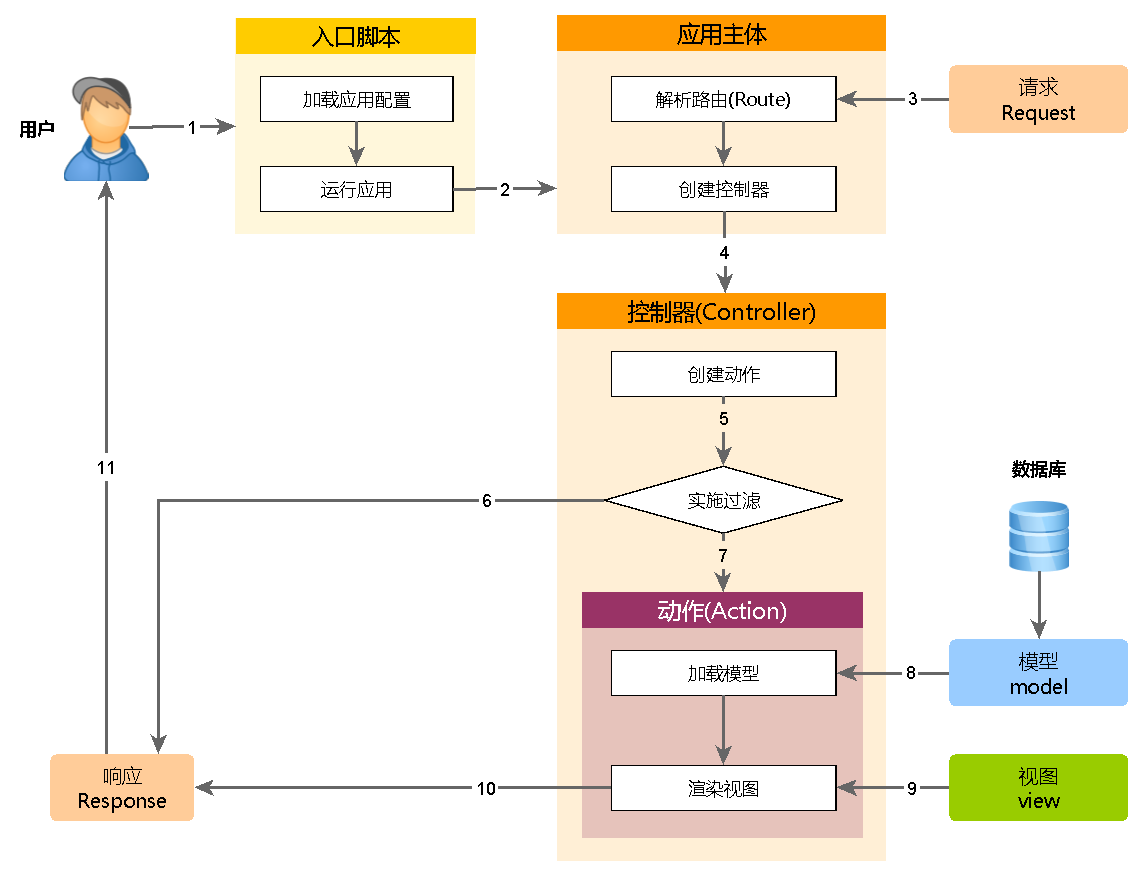
\includegraphics[width=\textwidth]{images/application-lifecycle.png}

在这个版块中,我们会更加详细地描述某些步骤的具体运作。



\label{runtime-bootstrapping.md}\section{启动引导(Bootstrapping)}
启动引导是指:在应用开始解析并处理新接受请求之前,一个预先准备环境的过程。启动引导会在两个地方具体进行:\hyperref[structure-entry-scripts.md]{入口脚本(Entry Script)}
和 \hyperref[structure-applications.md]{应用主体(application)}。

在\hyperref[structure-entry-scripts.md]{入口脚本}里,需注册各个类库的类文件自动加载器(Class Autoloader,简称自动加载器)。这主要包括通过其 \lstinline|autoload.php| 文件加载的
Composer 自动加载器,以及通过 \lstinline|Yii| 类加载的 Yii 自动加载器。之后,入口脚本会加载应用的
\hyperref[concept-configurations.md]{配置(configuration)}
并创建一个 \hyperref[structure-applications.md]{应用主体} 的实例。

在应用主体的构造函数中,会执行以下引导工作:

\begin{enumerate}
\item 调用 \texttt{yii{\allowbreak{}\textbackslash}base{\allowbreak{}\textbackslash}Application\allowbreak{}::\allowbreak{}preInit()}(预初始化)方法,配置一些高优先级的应用属性,比如 \texttt{yii{\allowbreak{}\textbackslash}base{\allowbreak{}\textbackslash}Application\allowbreak{}::\allowbreak{}basePath} 属性。
\item 注册\texttt{yii{\allowbreak{}\textbackslash}base{\allowbreak{}\textbackslash}Application\allowbreak{}::\allowbreak{}errorHandler}。
\item 通过给定的应用配置初始化应用的各属性。
\item 通过调用 \texttt{yii{\allowbreak{}\textbackslash}base{\allowbreak{}\textbackslash}Application\allowbreak{}::\allowbreak{}init()}(初始化)方法,它会顺次调用
\texttt{yii{\allowbreak{}\textbackslash}base{\allowbreak{}\textbackslash}Application\allowbreak{}::\allowbreak{}bootstrap()} 从而运行引导组件。\begin{itemize}
\item 加载扩展清单文件(extension manifest file) \lstinline|vendor/yiisoft/extensions.php|。
\item 创建并运行各个扩展声明的 \hyperref[structure-extensions.md::bootstrapping-classes]{引导组件(bootstrap components)}。
\item 创建并运行各个 \hyperref[structure-application-components.md]{应用组件} 以及在应用的 \hyperref[structure-applications.md::bootstrap]{Bootstrap 属性}中声明的各个
\hyperref[structure-modules.md]{模块(modules)组件}(如果有)。
\end{itemize}

\end{enumerate}
因为引导工作必须在处理\textbf{每一次}请求之前都进行一遍,因此让该过程尽可能轻量化就异常重要,请尽可能地优化这一步骤。

请尽量不要注册太多引导组件。只有他需要在 HTTP 请求处理的全部生命周期中都作用时才需要使用它。举一个用到它的范例:一个模块需要注册额外的 URL 解析规则,就应该把它列在应用的
\hyperref[structure-applications.md::bootstrap]{bootstrap 属性}之中,这样该 URL 解析规则才能在解析请求之前生效。(译者注:换言之,为了性能需要,除了 URL 
解析等少量操作之外,绝大多数组件都应该按需加载,而不是都放在引导过程中。)

在生产环境中,可以开启字节码缓存,比如 APC,来进一步最小化加载和解析 PHP 文件所需的时间。

一些大型应用都包含有非常复杂的应用\hyperref[concept-configurations.md]{配置},它们会被分割到许多更小的配置文件中。此时,可以考虑将整个配置数组缓存起来,并在入口脚本创建应用实例之前直接从缓存中加载。



\label{runtime-routing.md}\section{Routing}
When the \texttt{yii{\allowbreak{}\textbackslash}web{\allowbreak{}\textbackslash}Application\allowbreak{}::\allowbreak{}run()} method is called by the \hyperref[structure-entry-scripts.md]{entry script},
the first thing it does is to resolve the incoming request and instantiate an appropriate
\hyperref[structure-controllers.md]{controller action} to handle the request. This process is called \textit{routing}.

\subsection{Resolving Route \label{runtime-routing.md::resolving-route}}
The first step of routing is to parse the incoming request into a route which, as described in
the \hyperref[structure-controllers.md::routes]{Controllers} section, is used to address a controller action.
This is done by \texttt{yii{\allowbreak{}\textbackslash}web{\allowbreak{}\textbackslash}Request\allowbreak{}::\allowbreak{}resolve()} method of the \lstinline|request| application component.
The method invokes the \hyperref[runtime-url-handling.md]{URL manager} to do the actual request parsing work.

By default, if the incoming request contains a \lstinline|GET| parameter named \lstinline|r|, its value will be considered
as the route. However, if the \texttt{yii{\allowbreak{}\textbackslash}web{\allowbreak{}\textbackslash}UrlManager\allowbreak{}::\allowbreak{}enablePrettyUrl} is enabled,
more work will be done to determine the requested route. For more details, please refer to
the \hyperref[runtime-url-handling.md]{URL Parsing and Generation} section.

In case a route cannot be determined, the \lstinline|request| component will throw a \texttt{yii{\allowbreak{}\textbackslash}web{\allowbreak{}\textbackslash}NotFoundHttpException}.

\subsubsection{Default Route \label{runtime-routing.md::default-route}}
If an incoming request does not specify a route, which often happens to the request for homepages,
the route specified by \texttt{yii{\allowbreak{}\textbackslash}web{\allowbreak{}\textbackslash}Application\allowbreak{}::\allowbreak{}defaultRoute} will be used. The default value of this property
is \lstinline|site/index|, which refers to the \lstinline|index| action of the \lstinline|site| controller. You may customize this property
in the application configuration like the following:

\lstset{language=php}\begin{lstlisting}
return [
    // ...
    'defaultRoute' => 'main/index',
];
\end{lstlisting}
\subsubsection{\lstinline|catchAll| Route \label{runtime-routing.md::catchall-route}}
Sometimes, you may want to put your Web application in maintenance mode temporarily and display the same
informational page for all requests. There are many ways to accomplish this goal. But one of the simplest
ways is to configure the \texttt{yii{\allowbreak{}\textbackslash}web{\allowbreak{}\textbackslash}Application\allowbreak{}::\allowbreak{}catchAll} property like the following in the application configuration:

\lstset{language=php}\begin{lstlisting}
return [
    // ...
    'catchAll' => ['site/offline'],
];
\end{lstlisting}
The \lstinline|catchAll| property should take an array whose first element specifies a route, and
the rest of the elements (name-value pairs) specify the parameters to be bound to the action.

When the \lstinline|catchAll| property is set, it will replace any route resolved from the incoming requests.
With the above configuration, the same \lstinline|site/offline| action will be used to handle all incoming requests.

\subsection{Creating Action \label{runtime-routing.md::creating-action}}
Once the requested route is determined, the next step is to create the action object corresponding to the route.

The route is broken down into multiple parts by the slashes in it. For example, \lstinline|site/index| will be
broken into \lstinline|site| and \lstinline|index|. Each part is an ID which may refer to a module, a controller or an action.

Starting from the first part in the route, the application conducts the following steps to create modules (if any),
the controller and the action:

\begin{enumerate}
\item Set the application as the current module.
\item Check if the \texttt{yii{\allowbreak{}\textbackslash}base{\allowbreak{}\textbackslash}Module\allowbreak{}::\allowbreak{}controllerMap} of the current module contains the current ID.
If so, a controller object will be created according to the controller configuration found in the map,
and do Step 5 with the rest parts of the route.
\item Check if the ID refers to a module listed in the \texttt{yii{\allowbreak{}\textbackslash}base{\allowbreak{}\textbackslash}Module\allowbreak{}::\allowbreak{}modules} property of
the current module. If so, a module is created according to the configuration found in the module list,
and do Step 2 with the next part in the route under the context of the newly created module.
\item Treat the ID as a controller ID and create a controller object. Do the next step with the rest part of
the route.
\item The controller looks for the current ID in its \texttt{yii{\allowbreak{}\textbackslash}base{\allowbreak{}\textbackslash}Controller\allowbreak{}::\allowbreak{}actions()}. If found,
it creates an action according to the configuration found in the map. Otherwise, the controller will
attempt to create an inline action which is defined by an action method corresponding to the current ID.
\end{enumerate}
Among the above steps, if any error occurs, a \texttt{yii{\allowbreak{}\textbackslash}web{\allowbreak{}\textbackslash}NotFoundHttpException} will be thrown, indicating
failure of the routing.



\label{runtime-requests.md}\section{Requests}
Requests made to an application are represented in terms of \texttt{yii{\allowbreak{}\textbackslash}web{\allowbreak{}\textbackslash}Request} objects which provide information
such as request parameters, HTTP headers, cookies, etc. For a given request, you can get access to the corresponding
request object via the \lstinline|request| \hyperref[structure-application-components.md]{application component} which is an instance
of \texttt{yii{\allowbreak{}\textbackslash}web{\allowbreak{}\textbackslash}Request}, by default. In this section, we will describe how you can make use of this component in your applications.

\subsection{Request Parameters \label{runtime-requests.md::request-parameters}}
To get request parameters, you can call \texttt{yii{\allowbreak{}\textbackslash}web{\allowbreak{}\textbackslash}Request\allowbreak{}::\allowbreak{}get()} and \texttt{yii{\allowbreak{}\textbackslash}web{\allowbreak{}\textbackslash}Request\allowbreak{}::\allowbreak{}post()} methods
of the \lstinline|request| component. They return the values of \lstinline|$_GET| and \lstinline|$_POST|, respectively. For example,

\lstset{language=php}\begin{lstlisting}
$request = Yii::$app->request;

$get = $request->get(); 
// equivalent to: $get = $_GET;

$id = $request->get('id');   
// equivalent to: $id = isset($_GET['id']) ? $_GET['id'] : null;

$id = $request->get('id', 1);   
// equivalent to: $id = isset($_GET['id']) ? $_GET['id'] : 1;

$post = $request->post(); 
// equivalent to: $post = $_POST;

$name = $request->post('name');   
// equivalent to: $name = isset($_POST['name']) ? $_POST['name'] : null;

$name = $request->post('name', '');   
// equivalent to: $name = isset($_POST['name']) ? $_POST['name'] : '';
\end{lstlisting}
\begin{quote}Info: Instead of directly accessing \lstinline|$_GET| and \lstinline|$_POST| to retrieve the request parameters, it is recommended
  that you get them via the \lstinline|request| component like shown above. This will make writing tests easier because
  you can create a mock request component with faked request data.

\end{quote}
When implementing \hyperref[rest-quick-start.md]{RESTful APIs}, you often need to retrieve parameters that are submitted
via PUT, PATCH or other \hyperref[runtime-requests.md::::request-methods]{request methods}. You can get these parameters by calling
the \texttt{yii{\allowbreak{}\textbackslash}web{\allowbreak{}\textbackslash}Request\allowbreak{}::\allowbreak{}getBodyParam()} methods. For example,

\lstset{language=php}\begin{lstlisting}
$request = Yii::$app->request;

// returns all parameters
$params = $request->bodyParams;

// returns the parameter "id"
$param = $request->getBodyParam('id');
\end{lstlisting}
\begin{quote}Info: Unlike \lstinline|GET| parameters, parameters submitted via \lstinline|POST|, \lstinline|PUT|, \lstinline|PATCH| etc. are sent in the request body.
  The \lstinline|request| component will parse these parameters when you access them through the methods described above.
  You can customize the way how these parameters are parsed by configuring the \texttt{yii{\allowbreak{}\textbackslash}web{\allowbreak{}\textbackslash}Request\allowbreak{}::\allowbreak{}parsers} property.

\end{quote}
\subsection{Request Methods \label{runtime-requests.md::request-methods}}
You can get the HTTP method used by the current request via the expression \lstinline|Yii::$app->request->method|.
A whole set of boolean properties are also provided for you to check if the current method is of certain type.
For example,

\lstset{language=php}\begin{lstlisting}
$request = Yii::$app->request;

if ($request->isAjax) { // the request is an AJAX request }
if ($request->isGet)  { // the request method is GET }
if ($request->isPost) { // the request method is POST }
if ($request->isPut)  { // the request method is PUT }
\end{lstlisting}
\subsection{Request URLs \label{runtime-requests.md::request-urls}}
The \lstinline|request| component provides many ways of inspecting the currently requested URL. 

Assuming the URL being requested is \lstinline|http://example.com/admin/index.php/product?id=100|, you can get various
parts of this URL as summarized in the following:

\begin{itemize}
\item \texttt{yii{\allowbreak{}\textbackslash}web{\allowbreak{}\textbackslash}Request\allowbreak{}::\allowbreak{}url}: returns \lstinline|/admin/index.php/product?id=100|, which is the URL without the host info part. 
\item \texttt{yii{\allowbreak{}\textbackslash}web{\allowbreak{}\textbackslash}Request\allowbreak{}::\allowbreak{}absoluteUrl}: returns \lstinline|http://example.com/admin/index.php/product?id=100|,
which is the whole URL including the host info part.
\item \texttt{yii{\allowbreak{}\textbackslash}web{\allowbreak{}\textbackslash}Request\allowbreak{}::\allowbreak{}hostInfo}: returns \lstinline|http://example.com|, which is the host info part of the URL.
\item \texttt{yii{\allowbreak{}\textbackslash}web{\allowbreak{}\textbackslash}Request\allowbreak{}::\allowbreak{}pathInfo}: returns \lstinline|/product|, which is the part after the entry script and 
before the question mark (query string).
\item \texttt{yii{\allowbreak{}\textbackslash}web{\allowbreak{}\textbackslash}Request\allowbreak{}::\allowbreak{}queryString}: returns \lstinline|id=100|, which is the part after the question mark. 
\item \texttt{yii{\allowbreak{}\textbackslash}web{\allowbreak{}\textbackslash}Request\allowbreak{}::\allowbreak{}baseUrl}: returns \lstinline|/admin|, which is the part after the host info and before
the entry script name.
\item \texttt{yii{\allowbreak{}\textbackslash}web{\allowbreak{}\textbackslash}Request\allowbreak{}::\allowbreak{}scriptUrl}: returns \lstinline|/admin/index.php|, which is the URL without path info and query string.
\item \texttt{yii{\allowbreak{}\textbackslash}web{\allowbreak{}\textbackslash}Request\allowbreak{}::\allowbreak{}serverName}: returns \lstinline|example.com|, which is the host name in the URL.
\item \texttt{yii{\allowbreak{}\textbackslash}web{\allowbreak{}\textbackslash}Request\allowbreak{}::\allowbreak{}serverPort}: returns 80, which is the port used by the Web server.
\end{itemize}
\subsection{HTTP Headers \label{runtime-requests.md::http-headers}}
You can get the HTTP header information through the \texttt{yii{\allowbreak{}\textbackslash}web{\allowbreak{}\textbackslash}HeaderCollection} returned 
by the \texttt{yii{\allowbreak{}\textbackslash}web{\allowbreak{}\textbackslash}Request\allowbreak{}::\allowbreak{}headers} property. For example,

\lstset{language=php}\begin{lstlisting}
// $headers is an object of yii\web\HeaderCollection 
$headers = Yii::$app->request->headers;

// returns the Accept header value
$accept = $headers->get('Accept');

if ($headers->has('User-Agent')) { // there is User-Agent header }
\end{lstlisting}
The \lstinline|request| component also provides support for quickly accessing some commonly used headers, including

\begin{itemize}
\item \texttt{yii{\allowbreak{}\textbackslash}web{\allowbreak{}\textbackslash}Request\allowbreak{}::\allowbreak{}userAgent}: returns the value of the \lstinline|User-Agent| header.
\item \texttt{yii{\allowbreak{}\textbackslash}web{\allowbreak{}\textbackslash}Request\allowbreak{}::\allowbreak{}contentType}: returns the value of the \lstinline|Content-Type| header which indicates
the MIME type of the data in the request body.
\item \texttt{yii{\allowbreak{}\textbackslash}web{\allowbreak{}\textbackslash}Request\allowbreak{}::\allowbreak{}acceptableContentTypes}: returns the content MIME types acceptable by users.
The returned types ordered by the quality score. Types with the highest scores will be returned first.
\item \texttt{yii{\allowbreak{}\textbackslash}web{\allowbreak{}\textbackslash}Request\allowbreak{}::\allowbreak{}acceptableLanguages}: returns the languages acceptable by users.
The returned languages are ordered by their preference level. The first element represents the most preferred language.
\end{itemize}
If your application supports multiple languages and you want to display pages in the language that is the most preferred
by the end user, you may use the language negotiation method \texttt{yii{\allowbreak{}\textbackslash}web{\allowbreak{}\textbackslash}Request\allowbreak{}::\allowbreak{}getPreferredLanguage()}.
This method takes a list of languages supported by your application, compares them with \texttt{yii{\allowbreak{}\textbackslash}web{\allowbreak{}\textbackslash}Request\allowbreak{}::\allowbreak{}acceptableLanguages},
and returns the most appropriate language.

\begin{quote}Tip: You may also use the \texttt{yii{\allowbreak{}\textbackslash}filters{\allowbreak{}\textbackslash}ContentNegotiator} filter to dynamically determine 
  what content type and language should be used in the response. The filter implements the content negotiation
  on top the properties and methods described above.

\end{quote}
\subsection{Client Information \label{runtime-requests.md::client-information}}
You can get the host name and IP address of the client machine through \texttt{yii{\allowbreak{}\textbackslash}web{\allowbreak{}\textbackslash}Request\allowbreak{}::\allowbreak{}userHost}
and \texttt{yii{\allowbreak{}\textbackslash}web{\allowbreak{}\textbackslash}Request\allowbreak{}::\allowbreak{}userIP}, respectively. For example,

\lstset{language=php}\begin{lstlisting}
$userHost = Yii::$app->request->userHost;
$userIP = Yii::$app->request->userIP;
\end{lstlisting}


\label{runtime-responses.md}\section{Responses}
When an application finishes handling a \hyperref[runtime-requests.md]{request}, it generates a \texttt{yii{\allowbreak{}\textbackslash}web{\allowbreak{}\textbackslash}Response} object
and sends it to the end user. The response object contains information such as the HTTP status code, HTTP headers and body.
The ultimate goal of Web application development is essentially to build such response objects upon various requests.

In most cases you should mainly deal with the \lstinline|response| \hyperref[structure-application-components.md]{application component}
which is an instance of \texttt{yii{\allowbreak{}\textbackslash}web{\allowbreak{}\textbackslash}Response}, by default. However, Yii also allows you to create your own response
objects and send them to end users as we will explain in the following.

In this section, we will describe how to compose and send responses to end users. 

\subsection{Status Code \label{runtime-responses.md::status-code}}
One of the first things you would do when building a response is to state whether the request is successfully handled.
This is done by setting the \texttt{yii{\allowbreak{}\textbackslash}web{\allowbreak{}\textbackslash}Response\allowbreak{}::\allowbreak{}statusCode} property which can take one of the valid
HTTP status codes\footnote{\url{http://www.w3.org/Protocols/rfc2616/rfc2616-sec10.html}}. For example, to indicate the request
is successfully handled, you may set the status code to be 200, like the following:

\lstset{language=php}\begin{lstlisting}
Yii::$app->response->statusCode = 200;
\end{lstlisting}
However, in most cases you do not need to explicitly set the status code. This is because the default value
of \texttt{yii{\allowbreak{}\textbackslash}web{\allowbreak{}\textbackslash}Response\allowbreak{}::\allowbreak{}statusCode} is 200. And if you want to indicate the request is unsuccessful, you may
throw an appropriate HTTP exception like the following:

\lstset{language=php}\begin{lstlisting}
throw new \yii\web\NotFoundHttpException;
\end{lstlisting}
When the \hyperref[runtime-handling-errors.md]{error handler} catches an exception, it will extract the status code 
from the exception and assign it to the response. For the \texttt{yii{\allowbreak{}\textbackslash}web{\allowbreak{}\textbackslash}NotFoundHttpException} above, it is
associated with the HTTP status 404. The following HTTP exceptions are predefined in Yii:

\begin{itemize}
\item \texttt{yii{\allowbreak{}\textbackslash}web{\allowbreak{}\textbackslash}BadRequestHttpException}: status code 400.
\item \texttt{yii{\allowbreak{}\textbackslash}web{\allowbreak{}\textbackslash}ConflictHttpException}: status code 409.
\item \texttt{yii{\allowbreak{}\textbackslash}web{\allowbreak{}\textbackslash}ForbiddenHttpException}: status code 403.
\item \texttt{yii{\allowbreak{}\textbackslash}web{\allowbreak{}\textbackslash}GoneHttpException}: status code 410.
\item \texttt{yii{\allowbreak{}\textbackslash}web{\allowbreak{}\textbackslash}MethodNotAllowedHttpException}: status code 405.
\item \texttt{yii{\allowbreak{}\textbackslash}web{\allowbreak{}\textbackslash}NotAcceptableHttpException}: status code 406. 
\item \texttt{yii{\allowbreak{}\textbackslash}web{\allowbreak{}\textbackslash}NotFoundHttpException}: status code 404.
\item \texttt{yii{\allowbreak{}\textbackslash}web{\allowbreak{}\textbackslash}ServerErrorHttpException}: status code 500.
\item \texttt{yii{\allowbreak{}\textbackslash}web{\allowbreak{}\textbackslash}TooManyRequestsHttpException}: status code 429.
\item \texttt{yii{\allowbreak{}\textbackslash}web{\allowbreak{}\textbackslash}UnauthorizedHttpException}: status code 401.
\item \texttt{yii{\allowbreak{}\textbackslash}web{\allowbreak{}\textbackslash}UnsupportedMediaTypeHttpException}: status code 415.
\end{itemize}
If the exception that you want to throw is not among the above list, you may create one by extending
from \texttt{yii{\allowbreak{}\textbackslash}web{\allowbreak{}\textbackslash}HttpException}, or directly throw it with a status code, for example,

\lstset{language=php}\begin{lstlisting}
throw new \yii\web\HttpException(402);
\end{lstlisting}
\subsection{HTTP Headers \label{runtime-responses.md::http-headers}}
You can send HTTP headers by manipulating the \texttt{yii{\allowbreak{}\textbackslash}web{\allowbreak{}\textbackslash}Response\allowbreak{}::\allowbreak{}headers} in the \lstinline|response| component.
For example,

\lstset{language=php}\begin{lstlisting}
$headers = Yii::$app->response->headers;

// add a Pragma header. Existing Pragma headers will NOT be overwritten.
$headers->add('Pragma', 'no-cache');

// set a Pragma header. Any existing Pragma headers will be discarded.
$headers->set('Pragma', 'no-cache');

// remove Pragma header(s) and return the removed Pragma header values in array
$values = $headers->remove('Pragma');
\end{lstlisting}
\begin{quote}Info: Header names are case insensitive. And the newly registered headers are not sent to the user until
  the \texttt{yii{\allowbreak{}\textbackslash}web{\allowbreak{}\textbackslash}Response\allowbreak{}::\allowbreak{}send()} method is called.

\end{quote}
\subsection{Response Body \label{runtime-responses.md::response-body}}
Most responses should have a body which gives the content that you want to show to end users.

If you already have a formatted body string, you may assign it to the \texttt{yii{\allowbreak{}\textbackslash}web{\allowbreak{}\textbackslash}Response\allowbreak{}::\allowbreak{}content} property
of the response. For example,

\lstset{language=php}\begin{lstlisting}
Yii::$app->response->content = 'hello world!';
\end{lstlisting}
If your data needs to be formatted before sending it to end users, you should set both of the
\texttt{yii{\allowbreak{}\textbackslash}web{\allowbreak{}\textbackslash}Response\allowbreak{}::\allowbreak{}format} and \texttt{yii{\allowbreak{}\textbackslash}web{\allowbreak{}\textbackslash}Response\allowbreak{}::\allowbreak{}data} properties. The \texttt{yii{\allowbreak{}\textbackslash}web{\allowbreak{}\textbackslash}Response\allowbreak{}::\allowbreak{}format}
property specifies in which format the \texttt{yii{\allowbreak{}\textbackslash}web{\allowbreak{}\textbackslash}Response\allowbreak{}::\allowbreak{}data} should be formatted. For example,

\lstset{language=php}\begin{lstlisting}
$response = Yii::$app->response;
$response->format = \yii\web\Response::FORMAT_JSON;
$response->data = ['message' => 'hello world'];
\end{lstlisting}
Yii supports the following formats out of the box, each implemented by a \texttt{yii{\allowbreak{}\textbackslash}web{\allowbreak{}\textbackslash}ResponseFormatterInterface} class.
You can customize these formatters or add new ones by configuring the \texttt{yii{\allowbreak{}\textbackslash}web{\allowbreak{}\textbackslash}Response\allowbreak{}::\allowbreak{}formatters} property.

\begin{itemize}
\item \texttt{yii{\allowbreak{}\textbackslash}web{\allowbreak{}\textbackslash}Response\allowbreak{}::\allowbreak{}FORMAT\_HTML}: implemented by \texttt{yii{\allowbreak{}\textbackslash}web{\allowbreak{}\textbackslash}HtmlResponseFormatter}.
\item \texttt{yii{\allowbreak{}\textbackslash}web{\allowbreak{}\textbackslash}Response\allowbreak{}::\allowbreak{}FORMAT\_XML}: implemented by \texttt{yii{\allowbreak{}\textbackslash}web{\allowbreak{}\textbackslash}XmlResponseFormatter}.
\item \texttt{yii{\allowbreak{}\textbackslash}web{\allowbreak{}\textbackslash}Response\allowbreak{}::\allowbreak{}FORMAT\_JSON}: implemented by \texttt{yii{\allowbreak{}\textbackslash}web{\allowbreak{}\textbackslash}JsonResponseFormatter}.
\item \texttt{yii{\allowbreak{}\textbackslash}web{\allowbreak{}\textbackslash}Response\allowbreak{}::\allowbreak{}FORMAT\_JSONP}: implemented by \texttt{yii{\allowbreak{}\textbackslash}web{\allowbreak{}\textbackslash}JsonResponseFormatter}.
\end{itemize}
While response body can be set explicitly as shown above, in most cases you may set it implicitly by the return value
of \hyperref[structure-controllers.md]{action} methods. A common use case is like the following:

\lstset{language=php}\begin{lstlisting}
public function actionIndex()
{
    return $this->render('index');
}
\end{lstlisting}
The \lstinline|index| action above returns the rendering result of the \lstinline|index| view. The return value will be taken
by the \lstinline|response| component, formatted and then sent to end users.

Because by default, the response format is as \texttt{yii{\allowbreak{}\textbackslash}web{\allowbreak{}\textbackslash}Response\allowbreak{}::\allowbreak{}FORMAT\_HTML}, you should only return a string
in an action method. If you want to use a different response format, you should set it first before returning the data.
For example,

\lstset{language=php}\begin{lstlisting}
public function actionInfo()
{
    \Yii::$app->response->format = \yii\web\Response::FORMAT_JSON;
    return [
        'message' => 'hello world',
        'code' => 100,
    ];
}
\end{lstlisting}
As aforementioned, besides using the default \lstinline|response| application component, you can also create your own
response objects and send them to end users. You can do so by returning such object in an action method, like the following,

\lstset{language=php}\begin{lstlisting}
public function actionInfo()
{
    return \Yii::createObject([
        'class' => 'yii\web\Response',
        'format' => \yii\web\Response::FORMAT_JSON,
        'data' => [
            'message' => 'hello world',
            'code' => 100,
        ],
    ]);
}
\end{lstlisting}
\begin{quote}Note: If you are creating your own response objects, you will not be able to take advantage of the configurations
  that you set for the \lstinline|response| component in the application configuration. You can, however, use 
  \hyperref[concept-di-container.md]{dependency injection} to apply common configuration to your new response objects.

\end{quote}
\subsection{Browser Redirection \label{runtime-responses.md::browser-redirection}}
Browser redirection relies on sending a \lstinline|Location| HTTP header. Because this feature is commonly used, Yii provides
some special supports for it.

You can redirect the user browser to a URL by calling the \texttt{yii{\allowbreak{}\textbackslash}web{\allowbreak{}\textbackslash}Response\allowbreak{}::\allowbreak{}redirect()} method. The method
sets the appropriate \lstinline|Location| header with the given URL and returns the response object itself. In an action method,
you can call its shortcut version \texttt{yii{\allowbreak{}\textbackslash}web{\allowbreak{}\textbackslash}Controller\allowbreak{}::\allowbreak{}redirect()}. For example,

\lstset{language=php}\begin{lstlisting}
public function actionOld()
{
    return $this->redirect('http://example.com/new', 301);
}
\end{lstlisting}
In the above code, the action method returns the result of the \lstinline|redirect()| method. As explained before, the response
object returned by an action method will be used as the response sending to end users.

In places other than an action method, you should call \texttt{yii{\allowbreak{}\textbackslash}web{\allowbreak{}\textbackslash}Response\allowbreak{}::\allowbreak{}redirect()} directly followed by 
a call to the \texttt{yii{\allowbreak{}\textbackslash}web{\allowbreak{}\textbackslash}Response\allowbreak{}::\allowbreak{}send()} method to ensure no extra content will be appended to the response.

\lstset{language=php}\begin{lstlisting}
\Yii::$app->response->redirect('http://example.com/new', 301)->send();
\end{lstlisting}
\begin{quote}Info: By default, the \texttt{yii{\allowbreak{}\textbackslash}web{\allowbreak{}\textbackslash}Response\allowbreak{}::\allowbreak{}redirect()} method sets the response status code to be 302 which instructs
  the browser that the resource being requested is \textit{temporarily} located in a different URI. You can pass in a status
  code 301 to tell the browser that the resource has been \textit{permanently} relocated.

\end{quote}
When the current request is an AJAX request, sending a \lstinline|Location| header will not automatically cause the browser
redirection. To solve this problem, the \texttt{yii{\allowbreak{}\textbackslash}web{\allowbreak{}\textbackslash}Response\allowbreak{}::\allowbreak{}redirect()} method sets an \lstinline|X-Redirect| header with 
the redirection URL as its value. On the client side you may write JavaScript code to read this header value and
redirect the browser accordingly.

\begin{quote}Info: Yii comes with a \lstinline|yii.js| JavaScript file which provides a set of commonly used JavaScript utilities,
  including browser redirection based on the \lstinline|X-Redirect| header. Therefore, if you are using this JavaScript file
  (by registering the \texttt{yii{\allowbreak{}\textbackslash}web{\allowbreak{}\textbackslash}YiiAsset} asset bundle), you do not need to write anything to support AJAX redirection.

\end{quote}
\subsection{Sending Files \label{runtime-responses.md::sending-files}}
Like browser redirection, file sending is another feature that relies on specific HTTP headers. Yii provides
a set of methods to support various file sending needs. They all have built-in support for HTTP range header.

\begin{itemize}
\item \texttt{yii{\allowbreak{}\textbackslash}web{\allowbreak{}\textbackslash}Response\allowbreak{}::\allowbreak{}sendFile()}: sends an existing file to client.
\item \texttt{yii{\allowbreak{}\textbackslash}web{\allowbreak{}\textbackslash}Response\allowbreak{}::\allowbreak{}sendContentAsFile()}: sends a text string as a file to client.
\item \texttt{yii{\allowbreak{}\textbackslash}web{\allowbreak{}\textbackslash}Response\allowbreak{}::\allowbreak{}sendStreamAsFile()}: sends an existing file stream as a file to client. 
\end{itemize}
These methods have the same method signature with the response object as the return value. If the file
to be sent is very big, you should consider using \texttt{yii{\allowbreak{}\textbackslash}web{\allowbreak{}\textbackslash}Response\allowbreak{}::\allowbreak{}sendStreamAsFile()} because it is more
memory efficient. The following example shows how to send a file in a controller action:

\lstset{language=php}\begin{lstlisting}
public function actionDownload()
{
    return \Yii::$app->response->sendFile('path/to/file.txt');
}
\end{lstlisting}
If you are calling the file sending method in places other than an action method, you should also call
the \texttt{yii{\allowbreak{}\textbackslash}web{\allowbreak{}\textbackslash}Response\allowbreak{}::\allowbreak{}send()} method afterwards to ensure no extra content will be appended to the response.

\lstset{language=php}\begin{lstlisting}
\Yii::$app->response->sendFile('path/to/file.txt')->send();
\end{lstlisting}
Some Web servers have a special file sending support called \textit{X-Sendfile}. The idea is to redirect the
request for a file to the Web server which will directly serve the file. As a result, the Web application
can terminate earlier while the Web server is sending the file. To use this feature, you may call
the \texttt{yii{\allowbreak{}\textbackslash}web{\allowbreak{}\textbackslash}Response\allowbreak{}::\allowbreak{}xSendFile()}. The following list summarizes how to enable the \lstinline|X-Sendfile| feature
for some popular Web servers:

\begin{itemize}
\item Apache: X-Sendfile\footnote{\url{http://tn123.org/mod\_xsendfile}}
\item Lighttpd v1.4: X-LIGHTTPD-send-file\footnote{\url{http://redmine.lighttpd.net/projects/lighttpd/wiki/X-LIGHTTPD-send-file}}
\item Lighttpd v1.5: X-Sendfile\footnote{\url{http://redmine.lighttpd.net/projects/lighttpd/wiki/X-LIGHTTPD-send-file}}
\item Nginx: X-Accel-Redirect\footnote{\url{http://wiki.nginx.org/XSendfile}}
\item Cherokee: X-Sendfile and X-Accel-Redirect\footnote{\url{http://www.cherokee-project.com/doc/other\_goodies.html\#x-sendfile}}
\end{itemize}
\subsection{Sending Response \label{runtime-responses.md::sending-response}}
The content in a response is not sent to the user until the \texttt{yii{\allowbreak{}\textbackslash}web{\allowbreak{}\textbackslash}Response\allowbreak{}::\allowbreak{}send()} method is called.
By default, this method will be called automatically at the end of \texttt{yii{\allowbreak{}\textbackslash}base{\allowbreak{}\textbackslash}Application\allowbreak{}::\allowbreak{}run()}. You can, however,
explicitly call this method to force sending out the response immediately.

The \texttt{yii{\allowbreak{}\textbackslash}web{\allowbreak{}\textbackslash}Response\allowbreak{}::\allowbreak{}send()} method takes the following steps to send out a response:

\begin{enumerate}
\item Trigger the \texttt{yii{\allowbreak{}\textbackslash}web{\allowbreak{}\textbackslash}Response\allowbreak{}::\allowbreak{}EVENT\_BEFORE\_SEND} event.
\item Call \texttt{yii{\allowbreak{}\textbackslash}web{\allowbreak{}\textbackslash}Response\allowbreak{}::\allowbreak{}prepare()} to format \texttt{yii{\allowbreak{}\textbackslash}web{\allowbreak{}\textbackslash}Response\allowbreak{}::\allowbreak{}data} into 
\texttt{yii{\allowbreak{}\textbackslash}web{\allowbreak{}\textbackslash}Response\allowbreak{}::\allowbreak{}content}.
\item Trigger the \texttt{yii{\allowbreak{}\textbackslash}web{\allowbreak{}\textbackslash}Response\allowbreak{}::\allowbreak{}EVENT\_AFTER\_PREPARE} event.
\item Call \texttt{yii{\allowbreak{}\textbackslash}web{\allowbreak{}\textbackslash}Response\allowbreak{}::\allowbreak{}sendHeaders()} to send out the registered HTTP headers.
\item Call \texttt{yii{\allowbreak{}\textbackslash}web{\allowbreak{}\textbackslash}Response\allowbreak{}::\allowbreak{}sendContent()} to send out the response body content.
\item Trigger the \texttt{yii{\allowbreak{}\textbackslash}web{\allowbreak{}\textbackslash}Response\allowbreak{}::\allowbreak{}EVENT\_AFTER\_SEND} event.
\end{enumerate}
After the \texttt{yii{\allowbreak{}\textbackslash}web{\allowbreak{}\textbackslash}Response\allowbreak{}::\allowbreak{}send()} method is called once, any further call to this method will be ignored.
This means once the response is sent out, you will not be able to append more content to it.

As you can see, the \texttt{yii{\allowbreak{}\textbackslash}web{\allowbreak{}\textbackslash}Response\allowbreak{}::\allowbreak{}send()} method triggers several useful events. By responding to
these events, it is possible to adjust or decorate the response.



\label{runtime-sessions-cookies.md}\section{Sessions and Cookies}
Sessions and cookies allow data to be persisted across multiple user requests. In plain PHP, you may access them
through the global variables \lstinline|$_SESSION| and \lstinline|$_COOKIE|, respectively. Yii encapsulates sessions and cookies as objects
and thus allows you to access them in an object-oriented fashion with additional nice enhancements.

\subsection{Sessions \label{runtime-sessions-cookies.md::sessions}}
Like \hyperref[runtime-requests.md]{requests} and \hyperref[runtime-responses.md]{responses}, you can get access to sessions via
the \lstinline|session| \hyperref[structure-application-components.md]{application component} which is an instance of \texttt{yii{\allowbreak{}\textbackslash}web{\allowbreak{}\textbackslash}Session},
by default.

\subsubsection{Opening and Closing Sessions \label{runtime-sessions-cookies.md::opening-closing-sessions}}
To open and close a session, you can do the following:

\lstset{language=php}\begin{lstlisting}
$session = Yii::$app->session;

// check if a session is already open
if ($session->isActive) ...

// open a session
$session->open();

// close a session
$session->close();

// destroys all data registered to a session.
$session->destroy();
\end{lstlisting}
You can call the \texttt{yii{\allowbreak{}\textbackslash}web{\allowbreak{}\textbackslash}Session\allowbreak{}::\allowbreak{}open()} and \texttt{yii{\allowbreak{}\textbackslash}web{\allowbreak{}\textbackslash}Session\allowbreak{}::\allowbreak{}close()} multiple times
without causing errors. This is because internally the methods will first check if the session is already opened.

\subsubsection{Accessing Session Data \label{runtime-sessions-cookies.md::access-session-data}}
To access the data stored in session, you can do the following:

\lstset{language=php}\begin{lstlisting}
$session = Yii::$app->session;

// get a session variable. The following usages are equivalent:
$language = $session->get('language');
$language = $session['language'];
$language = isset($_SESSION['language']) ? $_SESSION['language'] : null;

// set a session variable. The following usages are equivalent:
$session->set('language', 'en-US');
$session['language'] = 'en-US';
$_SESSION['language'] = 'en-US';

// remove a session variable. The following usages are equivalent:
$session->remove('language');
unset($session['language']);
unset($_SESSION['language']);

// check if a session variable exists. The following usages are equivalent:
if ($session->has('language')) ...
if (isset($session['language'])) ...
if (isset($_SESSION['language'])) ...

// traverse all session variables. The following usages are equivalent:
foreach ($session as $name => $value) ...
foreach ($_SESSION as $name => $value) ...
\end{lstlisting}
\begin{quote}Info: When you access session data through the \lstinline|session| component, a session will be automatically opened
if it has not been done so before. This is different from accessing session data through \lstinline|$_SESSION|, which requires
an explicit call of \lstinline|session_start()|.

\end{quote}
When working with session data that are arrays, the \lstinline|session| component has a limitation which prevents you from
directly modifying an array element. For example,

\lstset{language=php}\begin{lstlisting}
$session = Yii::$app->session;

// the following code will NOT work
$session['captcha']['number'] = 5;
$session['captcha']['lifetime'] = 3600;

// the following code works:
$session['captcha'] = [
    'number' => 5,
    'lifetime' => 3600,
];

// the following code also works:
echo $session['captcha']['lifetime'];
\end{lstlisting}
You can use one of the following workarounds to solve this problem:

\lstset{language=php}\begin{lstlisting}
$session = Yii::$app->session;

// directly use $_SESSION (make sure Yii::$app->session->open() has been called)
$_SESSION['captcha']['number'] = 5;
$_SESSION['captcha']['lifetime'] = 3600;

// get the whole array out first, modify it and then save it back
$captcha = $session['captcha'];
$captcha['number'] = 5;
$captcha['lifetime'] = 3600;
$session['captcha'] = $captcha;

// use ArrayObject instead of array
$session['captcha'] = new \ArrayObject;
...
$session['captcha']['number'] = 5;
$session['captcha']['lifetime'] = 3600;

// store array data by keys with common prefix
$session['captcha.number'] = 5;
$session['captcha.lifetime'] = 3600;
\end{lstlisting}
For better performance and code readability, we recommend the last workaround. That is, instead of storing
an array as a single session variable, you store each array element as a session variable which shares the same
key prefix with other array elements.

\subsubsection{Custom Session Storage \label{runtime-sessions-cookies.md::custom-session-storage}}
The default \texttt{yii{\allowbreak{}\textbackslash}web{\allowbreak{}\textbackslash}Session} class stores session data as files on the server. Yii also provides the following
session classes implementing different session storage:

\begin{itemize}
\item \texttt{yii{\allowbreak{}\textbackslash}web{\allowbreak{}\textbackslash}DbSession}: stores session data in a database table.
\item \texttt{yii{\allowbreak{}\textbackslash}web{\allowbreak{}\textbackslash}CacheSession}: stores session data in a cache with the help of a configured \hyperref[caching-data.md::cache-components]{cache component}.
\item \texttt{yii{\allowbreak{}\textbackslash}redis{\allowbreak{}\textbackslash}Session}: stores session data using redis\footnote{\url{http://redis.io/}} as the storage medium.
\item \texttt{yii{\allowbreak{}\textbackslash}mongodb{\allowbreak{}\textbackslash}Session}: stores session data in a MongoDB\footnote{\url{http://www.mongodb.org/}}.
\end{itemize}
All these session classes support the same set of API methods. As a result, you can switch to use a different
session storage without the need to modify your application code that uses session.

\begin{quote}Note: If you want to access session data via \lstinline|$_SESSION| while using custom session storage, you must make
  sure that the session is already started by \texttt{yii{\allowbreak{}\textbackslash}web{\allowbreak{}\textbackslash}Session\allowbreak{}::\allowbreak{}open()}. This is because custom session storage
  handlers are registered within this method.

\end{quote}
To learn how to configure and use these component classes, please refer to their API documentation. Below is
an example showing how to configure \texttt{yii{\allowbreak{}\textbackslash}web{\allowbreak{}\textbackslash}DbSession} in the application configuration to use database table
as session storage:

\lstset{language=php}\begin{lstlisting}
return [
    'components' => [
        'session' => [
            'class' => 'yii\web\DbSession',
            // 'db' => 'mydb',  // the application component ID of the DB connection. Defaults to 'db'.
            // 'sessionTable' => 'my_session', // session table name. Defaults to 'session'.
        ],
    ],
];
\end{lstlisting}
You also need to create the following database table to store session data:

\lstset{language=sql}\begin{lstlisting}
CREATE TABLE session
(
    id CHAR(40) NOT NULL PRIMARY KEY,
    expire INTEGER,
    data BLOB
)
\end{lstlisting}
where `BLOB' refers to the BLOB-type of your preferred DBMS. Below are the BLOB type that can be used for some popular DBMS:

\begin{itemize}
\item MySQL: LONGBLOB
\item PostgreSQL: BYTEA
\item MSSQL: BLOB
\end{itemize}
\begin{quote}Note: According to the php.ini setting of \lstinline|session.hash_function|, you may need to adjust
  the length of the \lstinline|id| column. For example, if \lstinline|session.hash_function=sha256|, you should use
  length 64 instead of 40.

\end{quote}
\subsubsection{Flash Data \label{runtime-sessions-cookies.md::flash-data}}
Flash data is a special kind of session data which, once set in one request, will only be available during
the next request and will be automatically deleted afterwards. Flash data is most commonly used to implement
messages that should only be displayed to end users once, such as a confirmation message displayed after
a user successfully submits a form.

You can set and access flash data through the \lstinline|session| application component. For example,

\lstset{language=php}\begin{lstlisting}
$session = Yii::$app->session;

// Request #1
// set a flash message named as "postDeleted"
$session->setFlash('postDeleted', 'You have successfully deleted your post.');

// Request #2
// display the flash message named "postDeleted"
echo $session->getFlash('postDeleted');

// Request #3
// $result will be false since the flash message was automatically deleted
$result = $session->hasFlash('postDeleted');
\end{lstlisting}
Like regular session data, you can store arbitrary data as flash data.

When you call \texttt{yii{\allowbreak{}\textbackslash}web{\allowbreak{}\textbackslash}Session\allowbreak{}::\allowbreak{}setFlash()}, it will overwrite any existing flash data that has the same name.
To append new flash data to the existing one(s) of the same name, you may call \texttt{yii{\allowbreak{}\textbackslash}web{\allowbreak{}\textbackslash}Session\allowbreak{}::\allowbreak{}addFlash()} instead.
For example:

\lstset{language=php}\begin{lstlisting}
$session = Yii::$app->session;

// Request #1
// add a few flash messages under the name of "alerts"
$session->addFlash('alerts', 'You have successfully deleted your post.');
$session->addFlash('alerts', 'You have successfully added a new friend.');
$session->addFlash('alerts', 'You are promoted.');

// Request #2
// $alerts is an array of the flash messages under the name of "alerts"
$alerts = $session->getFlash('alerts');
\end{lstlisting}
\begin{quote}Note: Try not to use \texttt{yii{\allowbreak{}\textbackslash}web{\allowbreak{}\textbackslash}Session\allowbreak{}::\allowbreak{}setFlash()} together with \texttt{yii{\allowbreak{}\textbackslash}web{\allowbreak{}\textbackslash}Session\allowbreak{}::\allowbreak{}addFlash()} for flash data
  of the same name. This is because the latter method will automatically turn the flash data into an array so that it
  can append new flash data of the same name. As a result, when you call \texttt{yii{\allowbreak{}\textbackslash}web{\allowbreak{}\textbackslash}Session\allowbreak{}::\allowbreak{}getFlash()}, you may
  find sometimes you are getting an array while sometimes you are getting a string, depending on the order of
  the invocation of these two methods.

\end{quote}
\subsection{Cookies \label{runtime-sessions-cookies.md::cookies}}
Yii represents each cookie as an object of \texttt{yii{\allowbreak{}\textbackslash}web{\allowbreak{}\textbackslash}Cookie}. Both \texttt{yii{\allowbreak{}\textbackslash}web{\allowbreak{}\textbackslash}Request} and \texttt{yii{\allowbreak{}\textbackslash}web{\allowbreak{}\textbackslash}Response}
maintain a collection of cookies via the property named \lstinline|cookies|. The cookie collection in the former represents
the cookies submitted in a request, while the cookie collection in the latter represents the cookies that are to
be sent to the user.

\subsubsection{Reading Cookies \label{runtime-sessions-cookies.md::reading-cookies}}
You can get the cookies in the current request using the following code:

\lstset{language=php}\begin{lstlisting}
// get the cookie collection (yii\web\CookieCollection) from "request" component
$cookies = Yii::$app->request->cookies;

// get the "language" cookie value. If the cookie does not exist, return "en" as the default value.
$language = $cookies->getValue('language', 'en');

// an alternative way of getting the "language" cookie value
if (($cookie = $cookies->get('language')) !== null) {
    $language = $cookie->value;
}

// you may also use $cookies like an array
if (isset($cookies['language'])) {
    $language = $cookies['language']->value;
}

// check if there is a "language" cookie
if ($cookies->has('language')) ...
if (isset($cookies['language'])) ...
\end{lstlisting}
\subsubsection{Sending Cookies \label{runtime-sessions-cookies.md::sending-cookies}}
You can send cookies to end users using the following code:

\lstset{language=php}\begin{lstlisting}
// get the cookie collection (yii\web\CookieCollection) from "response" component
$cookies = Yii::$app->response->cookies;

// add a new cookie to the response to be sent
$cookies->add(new \yii\web\Cookie([
    'name' => 'language',
    'value' => 'zh-CN',
]));

// remove a cookie
$cookies->remove('language');
// equivalent to the following
unset($cookies['language']);
\end{lstlisting}
Besides the \texttt{yii{\allowbreak{}\textbackslash}web{\allowbreak{}\textbackslash}Cookie\allowbreak{}::\allowbreak{}name}, \texttt{yii{\allowbreak{}\textbackslash}web{\allowbreak{}\textbackslash}Cookie\allowbreak{}::\allowbreak{}value} properties shown in the above
examples, the \texttt{yii{\allowbreak{}\textbackslash}web{\allowbreak{}\textbackslash}Cookie} class also defines other properties to fully represent all possible information
of cookies, such as \texttt{yii{\allowbreak{}\textbackslash}web{\allowbreak{}\textbackslash}Cookie\allowbreak{}::\allowbreak{}domain}, \texttt{yii{\allowbreak{}\textbackslash}web{\allowbreak{}\textbackslash}Cookie\allowbreak{}::\allowbreak{}expire}. You may configure these
properties as needed to prepare a cookie and then add it to the response's cookie collection.

\begin{quote}Note: For better security, the default value of \texttt{yii{\allowbreak{}\textbackslash}web{\allowbreak{}\textbackslash}Cookie\allowbreak{}::\allowbreak{}httpOnly} is set true. This helps mitigate
the risk of client side script accessing the protected cookie (if the browser supports it). You may read
the httpOnly wiki article\footnote{\url{https://www.owasp.org/index.php/HttpOnly}} for more details.

\end{quote}
\subsubsection{Cookie Validation \label{runtime-sessions-cookies.md::cookie-validation}}
When you are reading and sending cookies through the \lstinline|request| and \lstinline|response| components like shown in the last
two subsections, you enjoy the added security of cookie validation which protects cookies from being modified
on the client side. This is achieved by signing each cookie with a hash string, which allows the application to
tell if a cookie is modified on the client side or not. If so, the cookie will NOT be accessible through the
\texttt{yii{\allowbreak{}\textbackslash}web{\allowbreak{}\textbackslash}Request\allowbreak{}::\allowbreak{}cookies} of the \lstinline|request| component.

\begin{quote}Note: Cookie validation only protects cookie values from being modified. If a cookie fails the validation, 
you may still access it through \lstinline|$_COOKIE|. This is because third-party libraries may manipulate cookies 
in their own way, which does not involve cookie validation.

\end{quote}
Cookie validation is enabled by default. You can disable it by setting the \texttt{yii{\allowbreak{}\textbackslash}web{\allowbreak{}\textbackslash}Request\allowbreak{}::\allowbreak{}enableCookieValidation}
property to be false, although we strongly recommend you do not do so.

\begin{quote}Note: Cookies that are directly read/sent via \lstinline|$_COOKIE| and \lstinline|setcookie()| will NOT be validated.

\end{quote}
When using cookie validation, you must specify a \texttt{yii{\allowbreak{}\textbackslash}web{\allowbreak{}\textbackslash}Request\allowbreak{}::\allowbreak{}cookieValidationKey} that will be used to generate
the aforementioned hash strings. You can do so by configuring the \lstinline|request| component in the application configuration:

\lstset{language=php}\begin{lstlisting}
return [
    'components' => [
        'request' => [
            'cookieValidationKey' => 'fill in a secret key here',
        ],
    ],
];
\end{lstlisting}
\begin{quote}Info: \texttt{yii{\allowbreak{}\textbackslash}web{\allowbreak{}\textbackslash}Request\allowbreak{}::\allowbreak{}cookieValidationKey} is critical to your application's security.
  It should only be known to people you trust. Do not store it in version control system.

\end{quote}


\label{runtime-url-handling.md}\section{URL Parsing and Generation}
\begin{quote}Note: This section is under development.

\end{quote}
The concept of \textit{URL management} in Yii is fairly simple: the application simply uses internal routes and parameters everywhere. The framework itself will then translate routes into URLs, and vice versa, according to the URL manager's configuration. This approach allows you to make site-wide changes to URLs merely by
editing a single configuration file, without ever touching any application code.

\subsection{Internal Routes}
When implementing an application using Yii, you'll deal with \textit{internal} routes, often referred to as ``routes and parameters''.
Each controller and controller action has a corresponding internal route, such as \lstinline|site/index| or \lstinline|user/create|.

In the first example, \lstinline|site| is the \textit{controller ID}, while \lstinline|index| is the \textit{action ID}. In the
second example, \lstinline|user| is the controller ID and \lstinline|create| is the action ID. 

If the controller belongs to a \textit{module}, the
internal route is prefixed with the module ID: for example, \lstinline|blog/post/index| represents a blog module, the module's \lstinline|post| 
controller, and the \lstinline|index| action.

\subsection{Creating URLs}
The most important rule for creating URLs in your site is to always do so through the URL manager. The URL manager is a built-in application component fittingly named \lstinline|urlManager|. This component is accessible from both web and console applications via
\lstinline|\Yii::$app->urlManager|. The component makes available two methods for creating URLs:

\begin{itemize}
\item \lstinline|createUrl($params)|
\item \lstinline|createAbsoluteUrl($params, $schema = null)|
\end{itemize}
The \lstinline|createUrl| method creates an URL relative to the application root, such as \lstinline|/index.php/site/index/|.
The \lstinline|createAbsoluteUrl| method creates an URL that beings with with the proper protocol and hostname:
\lstinline|http://www.example.com/index.php/site/index|. Relative URLs, and the \lstinline|createUrl| method are suitable for internal application URLs, while absolute URLs, and the \lstinline|createAbsoluteUrl| method, are appropriate when you need to create URLs for external resources, such as connecting to third party services, sending email,
generating RSS feeds, etc.

Both methods can be passed parameters used to further customize the URL, such as appending values to pass along as part of the request.

Some examples of these two methods:

\lstset{language=php}\begin{lstlisting}
echo \Yii::$app->urlManager->createUrl(['site/page', 'id' => 'about']);
// /index.php/site/page/id/about/
echo \Yii::$app->urlManager->createUrl(['date-time/fast-forward', 'id' => 105])
// /index.php?r=date-time/fast-forward&id=105
echo \Yii::$app->urlManager->createAbsoluteUrl('blog/post/index');
// http://www.example.com/index.php/blog/post/index/
\end{lstlisting}
The exact format of the resuting URL depends on how the URL manager is configured. The above
examples could also output:

\begin{itemize}
\item \lstinline|/site/page/id/about/|
\item \lstinline|/index.php?r=site/page&id=about|
\item \lstinline|/index.php?r=date-time/fast-forward&id=105|
\item \lstinline|/index.php/date-time/fast-forward?id=105|
\item \lstinline|http://www.example.com/blog/post/index/|
\item \lstinline|http://www.example.com/index.php?r=blog/post/index|
\end{itemize}
In order to simplify URL creation, Yii has the \texttt{yii{\allowbreak{}\textbackslash}helpers{\allowbreak{}\textbackslash}Url} helper. Assuming the current URL is \lstinline|/index.php?r=management/default/users&id=10|, the following
shows how the \lstinline|Url| helper works:

\lstset{language=php}\begin{lstlisting}
use yii\helpers\Url;

// currently active route
// /index.php?r=management/default/users
echo Url::to('');

// same controller, different action
// /index.php?r=management/default/page&id=contact
echo Url::toRoute(['page', 'id' => 'contact']);

// same module, different controller and action
// /index.php?r=management/post/index
echo Url::toRoute('post/index');

// absolute route no matter what controller is making this call
// /index.php?r=site/index
echo Url::toRoute('/site/index');

// url for the case sensitive action `actionHiTech` of the current controller
// /index.php?r=management/default/hi-tech
echo Url::toRoute('hi-tech');

// url for action the case sensitive controller, `DateTimeController::actionFastForward`
// /index.php?r=date-time/fast-forward&id=105
echo Url::toRoute(['/date-time/fast-forward', 'id' => 105]);

// get URL from alias
// http://google.com/
Yii::setAlias('@google', 'http://google.com/');
echo Url::to('@google');

// get home URL
// /index.php?r=site/index
echo Url::home();

Url::remember(); // save URL to be used later
Url::previous(); // get previously saved URL
\end{lstlisting}
\begin{quote}\textbf{Tip}: In order to generate a URL containing a hashtag, for example \lstinline|/index.php?r=site/page&id=100#title|, you need to
  specify the parameter named \lstinline|#| using \lstinline|Url::to(['post/read', 'id' => 100, '#' => 'title'])|.

\end{quote}
There's also the \lstinline|Url::canonical()| method that allows you to generate
canonical URLs\footnote{\url{https://en.wikipedia.org/wiki/Canonical\_link\_element}} for the current action.
This method ignores all action parameters except for ones specifically passed via action arguments:

\lstset{language=php}\begin{lstlisting}
namespace app\controllers;

use yii\web\Controller;
use yii\helpers\Url;

class CanonicalController extends Controller
{
    public function actionTest($page)
    {
        echo Url::canonical();
    }
}
\end{lstlisting}
When accessed as \lstinline|/index.php?r=canonical/test&page=hello&number=42|, the canonical URL will be \lstinline|/index.php?r=canonical/test&page=hello|.

\subsection{Customizing URLs}
By default, Yii uses a query string format for URLs, such as \lstinline|/index.php?r=news/view&id=100|. In order to make URLs
human-friendly (i.e., more legible), you need to configure the \lstinline|urlManager| component in the application's configuration
file. Enabling ``pretty'' URLs will convert the query string format to a directory-based format: \lstinline|/index.php/news/view?id=100|.

Disabling the \lstinline|showScriptName| parameter further customizes the URL such that \lstinline|index.php| will be omitted. Here's the relevant part of
the application's configuration file:

\lstset{language=php}\begin{lstlisting}
<?php
return [
    // ...
    'components' => [
        'urlManager' => [
            'enablePrettyUrl' => true,
            'showScriptName' => false,
        ],
    ],
];
\end{lstlisting}
Note that this configuration will only work if the web server has also been properly configured for Yii, see
\hyperref[start-installation.md::recommended-apache-configuration]{installation}.

\subsubsection{Named Parameters}
A rule can be associated with a few \lstinline|GET| parameters. These \lstinline|GET| parameters appear in the rule's pattern as special tokens in the following format:

\lstset{language={}}\begin{lstlisting}
<ParameterName:ParameterPattern>
\end{lstlisting}
\lstinline|ParameterName| is a name of a \lstinline|GET| parameter, and the optional \lstinline|ParameterPattern| is the regular expression that should
be used to match the value of the \lstinline|GET| parameter. When \lstinline|ParameterPattern| is omitted, it means the parameter
should match any characters except \lstinline|/|. When creating a URL, these parameter tokens will be replaced with the
corresponding parameter values; when parsing a URL, the corresponding GET parameters will be populated with the parsed results.

Let's use some examples to explain how URL rules work. Asusuming that the rule set consists of three rules:

\lstset{language=php}\begin{lstlisting}
[
    'posts'=>'post/list',
    'post/<id:\d+>'=>'post/read',
    'post/<year:\d{4}>/<title>'=>'post/read',
]
\end{lstlisting}
\begin{itemize}
\item Calling \lstinline|Url::toRoute('post/list')| generates \lstinline|/index.php/posts|. The first rule is applied.
\item Calling \lstinline|Url::toRoute(['post/read', 'id' => 100])| generates \lstinline|/index.php/post/100|. The second rule is applied.
\item Calling \lstinline|Url::toRoute(['post/read', 'year' => 2008, 'title' => 'a sample post'])| generates
\lstinline|/index.php/post/2008/a%20sample%20post|. The third rule is applied.
\item Calling \lstinline|Url::toRoute('post/read')| generates \lstinline|/index.php/post/read|. None of the rules is applied; convention is used instead.
\end{itemize}
In summary, when using \lstinline|createUrl| to generate a URL, the route and the \lstinline|GET| parameters passed to the method are used to
decide which URL rule will be applied. If every parameter associated with a rule can be found in the \lstinline|GET| parameters passed
to \lstinline|createUrl|, and if the route of the rule also matches the route parameter, the rule will be used to generate the URL.

If the \lstinline|GET| parameters passed to \lstinline|Url::toRoute| are more than those required by a rule, the additional parameters will
appear in the query string. For example, the call \lstinline|Url::toRoute(['post/read', 'id' => 100, 'year' => 2008])|, will
generate \lstinline|/index.php/post/100?year=2008|.

As mentioned earlier, the other purpose of URL rules is to parse the requesting URLs. Naturally, this is the inverse of URL creation. For example, when a user requests for \lstinline|/index.php/post/100|, the second rule in the above example
will apply, which resolves to the route \lstinline|post/read| with the \lstinline|GET| parameter \lstinline|['id' => 100]| (accessible via
\lstinline|Yii::$app->request->get('id')|).

\subsubsection{Parameterizing Routes}
Rules may also make use of named parameters as part of a route. Named parameters allow a rule to be applied to multiple routes based
on matching criteria. Named parameters may also help reduce the number of rules needed for an application, and thus improve the overall
performance.

The following example rules illustrate how to parameterize routes with named parameters:

\lstset{language=php}\begin{lstlisting}
[
    '<controller:(post|comment)>/<id:\d+>/<action:(create|update|delete)>' => '<controller>/<action>',
    '<controller:(post|comment)>/<id:\d+>' => '<controller>/read',
    '<controller:(post|comment)>s' => '<controller>/list',
]
\end{lstlisting}
In the above example, two named parameters are found in the route part of the rules: \lstinline|controller| and \lstinline|action|. The former matches a controller ID that's either ``post'' or ``comment'', while the latter matches an action ID that could be ``create'', ``update'', or ``delete''. You may name the parameters differently as long as they do not conflict with any GET parameters that may appear in your URLs.

Using the above rules, the URL \lstinline|/index.php/post/123/create| will be parsed as the route \lstinline|post/create| with \lstinline|GET| parameter
\lstinline|id=123|. Given the route \lstinline|comment/list| and \lstinline|GET| parameter \lstinline|page=2|, Yii can create a URL \lstinline|/index.php/comments?page=2|.

\subsubsection{Parameterizing Hostnames}
It is also possible to include hostnames in the rules for parsing and creating URLs. One may extract part of the hostname
to be a \lstinline|GET| parameter. This is especially useful for handling subdomains. For example, the URL
\lstinline|http://admin.example.com/en/profile| may be parsed into GET parameters \lstinline|user=admin| and \lstinline|lang=en|. On the other hand,
rules with hostnames may also be used to create URLs with parameterized hostnames.

In order to use parameterized hostnames, simply declare the URL rules while including the host info:

\lstset{language=php}\begin{lstlisting}
[
    'http://<user:\w+>.example.com/<lang:\w+>/profile' => 'user/profile',
]
\end{lstlisting}
In the above example, the first segment of the hostname is treated as the ``user'' parameter while the first segment
of the pat is treated as the ``lang'' parameter. The rule corresponds to the \lstinline|user/profile| route.

Note that \texttt{yii{\allowbreak{}\textbackslash}web{\allowbreak{}\textbackslash}UrlManager\allowbreak{}::\allowbreak{}showScriptName} will not take effect when a URL is being created using a rule with a parameterized hostname.

Also note that any rule with a parameterized hostname should NOT contain the subfolder if the application is under
a subfolder of the web root. For example, if the application is under \lstinline|http://www.example.com/sandbox/blog|, then you
should still use the same URL rule as described above without the subfolder \lstinline|sandbox/blog|.

\subsubsection{Faking URL Suffix}
\lstset{language=php}\begin{lstlisting}
<?php
return [
    // ...
    'components' => [
        'urlManager' => [
            'suffix' => '.html',
        ],
    ],
];
\end{lstlisting}
\subsubsection{Handling REST requests}
TBD:

\begin{itemize}
\item RESTful routing: \texttt{yii{\allowbreak{}\textbackslash}filters{\allowbreak{}\textbackslash}VerbFilter}, \texttt{yii{\allowbreak{}\textbackslash}web{\allowbreak{}\textbackslash}UrlManager\allowbreak{}::\allowbreak{}\$rules}
\item Json API:\begin{itemize}
\item response: \texttt{yii{\allowbreak{}\textbackslash}web{\allowbreak{}\textbackslash}Response\allowbreak{}::\allowbreak{}format}
\item request: \texttt{yii{\allowbreak{}\textbackslash}web{\allowbreak{}\textbackslash}Request\allowbreak{}::\allowbreak{}\$parsers}, \texttt{yii{\allowbreak{}\textbackslash}web{\allowbreak{}\textbackslash}JsonParser}
\end{itemize}

\end{itemize}
\subsection{URL parsing}
Complimentary to creating URLs Yii also handles transforming custom URLs back into internal routes and parameters.

\subsubsection{Strict URL parsing}
By default if there's no custom rule for a URL and the URL matches the default format such as \lstinline|/site/page|, Yii tries to run the corresponding controller's action. This behavior can be disabled so if there's no custom rule match, a 404 not found error will be produced immediately.

\lstset{language=php}\begin{lstlisting}
<?php
return [
    // ...
    'components' => [
        'urlManager' => [
            'enableStrictParsing' => true,
        ],
    ],
];
\end{lstlisting}
\subsection{Creating your own rule classes}
\texttt{yii{\allowbreak{}\textbackslash}web{\allowbreak{}\textbackslash}UrlRule} class is used for both parsing URL into parameters and creating URL based on parameters. Despite
the fact that default implementation is flexible enough for the majority of projects, there are situations when using
your own rule class is the best choice. For example, in a car dealer website, we may want to support the URL format like
\lstinline|/Manufacturer/Model|, where \lstinline|Manufacturer| and \lstinline|Model| must both match some data in a database table. The default rule
class will not work because it mostly relies on statically declared regular expressions which have no database knowledge.

We can write a new URL rule class by extending from \texttt{yii{\allowbreak{}\textbackslash}web{\allowbreak{}\textbackslash}UrlRule} and use it in one or multiple URL rules. Using
the above car dealer website as an example, we may declare the following URL rules in application config:

\lstset{language=php}\begin{lstlisting}
// ...
'components' => [
    'urlManager' => [
        'rules' => [
            '<action:(login|logout|about)>' => 'site/<action>',

            // ...

            ['class' => 'app\components\CarUrlRule', 'connectionID' => 'db', /* ... */],
        ],
    ],
],
\end{lstlisting}
In the above, we use the custom URL rule class \lstinline|CarUrlRule| to handle
the URL format \lstinline|/Manufacturer/Model|. The class can be written like the following:

\lstset{language=php}\begin{lstlisting}
namespace app\components;

use yii\web\UrlRule;

class CarUrlRule extends UrlRule
{
    public $connectionID = 'db';

    public function init()
    {
        if ($this->name === null) {
            $this->name = __CLASS__;
        }
    }

    public function createUrl($manager, $route, $params)
    {
        if ($route === 'car/index') {
            if (isset($params['manufacturer'], $params['model'])) {
                return $params['manufacturer'] . '/' . $params['model'];
            } elseif (isset($params['manufacturer'])) {
                return $params['manufacturer'];
            }
        }
        return false;  // this rule does not apply
    }

    public function parseRequest($manager, $request)
    {
        $pathInfo = $request->getPathInfo();
        if (preg_match('%^(\w+)(/(\w+))?$%', $pathInfo, $matches)) {
            // check $matches[1] and $matches[3] to see
            // if they match a manufacturer and a model in the database
            // If so, set $params['manufacturer'] and/or $params['model']
            // and return ['car/index', $params]
        }
        return false;  // this rule does not apply
    }
}
\end{lstlisting}
Besides the above usage, custom URL rule classes can also be implemented
for many other purposes. For example, we can write a rule class to log the URL parsing
and creation requests. This may be useful during development stage. We can also
write a rule class to display a special 404 error page in case all other URL rules fail
to resolve the current request. Note that in this case, the rule of this special class
must be declared as the last rule.



\label{runtime-handling-errors.md}\section{Handling Errors}
Yii includes a built-in \texttt{yii{\allowbreak{}\textbackslash}web{\allowbreak{}\textbackslash}ErrorHandler} which makes error handling a much more pleasant
experience than before. In particular, the Yii error handler does the followings to improve error handling:

\begin{itemize}
\item All non-fatal PHP errors (e.g. warnings, notices) are converted into catchable exceptions.
\item Exceptions and fatal PHP errors are displayed with detailed call stack information and source code lines
in debug mode.
\item Support using a dedicated \hyperref[structure-actions.md]{controller action} to display errors.
\item Support different error response formats.
\end{itemize}
The \texttt{yii{\allowbreak{}\textbackslash}web{\allowbreak{}\textbackslash}ErrorHandler} is enabled by default. You may disable it by defining the constant
\lstinline|YII_ENABLE_ERROR_HANDLER| to be false in the \hyperref[structure-entry-scripts.md]{entry script} of your application.

\subsection{Using Error Handler \label{runtime-handling-errors.md::using-error-handler}}
The \texttt{yii{\allowbreak{}\textbackslash}web{\allowbreak{}\textbackslash}ErrorHandler} is registered as an \hyperref[structure-application-components.md]{application component} named \lstinline|errorHandler|.
You may configure it in the application configuration like the following:

\lstset{language=php}\begin{lstlisting}
return [
    'components' => [
        'errorHandler' => [
            'maxSourceLines' => 20,
        ],
    ],
];
\end{lstlisting}
With the above configuration, the number of source code lines to be displayed in exception pages will be up to 20.

As aforementioned, the error handler turns all non-fatal PHP errors into catchable exceptions. This means you can
use the following code to deal with PHP errors:

\lstset{language=php}\begin{lstlisting}
use Yii;
use yii\base\ErrorException;

try {
    10/0;
} catch (ErrorException $e) {
    Yii::warning("Division by zero.");
}

// execution continues...
\end{lstlisting}
If you want to show an error page telling the user that his request is invalid or unexpected, you may simply
throw an \texttt{yii{\allowbreak{}\textbackslash}web{\allowbreak{}\textbackslash}HttpException}, such as \texttt{yii{\allowbreak{}\textbackslash}web{\allowbreak{}\textbackslash}NotFoundHttpException}. The error handler
will correctly set the HTTP status code of the response and use an appropriate error view to display the error
message.

\lstset{language=php}\begin{lstlisting}
use yii\web\NotFoundHttpException;

throw new NotFoundHttpException();
\end{lstlisting}
\subsection{Customizing Error Display \label{runtime-handling-errors.md::customizing-error-display}}
The \texttt{yii{\allowbreak{}\textbackslash}web{\allowbreak{}\textbackslash}ErrorHandler} adjusts error display according to the value of the constant \lstinline|YII_DEBUG|.
When \lstinline|YII_DEBUG| is true (meaning in debug mode), the error handler will display exceptions with detailed call
stack information and source code lines to help easier debugging. And when \lstinline|YII_DEBUG| is false, only the error
message will be displayed to prevent from revealing sensitive information of the application.

\begin{quote}Info: If an exception is a descendant of \texttt{yii{\allowbreak{}\textbackslash}base{\allowbreak{}\textbackslash}UserException}, no call stack will be displayed regardless
the value of \lstinline|YII_DEBUG|. This is because such exceptions are considered to be caused by user mistakes and the
developers do not need to fix anything.

\end{quote}
By default, the \texttt{yii{\allowbreak{}\textbackslash}web{\allowbreak{}\textbackslash}ErrorHandler} displays errors using two \hyperref[structure-views.md]{views}:

\begin{itemize}
\item \lstinline|@yii/views/errorHandler/error.php|: used when errors should be displayed WITHOUT call stack information.
When \lstinline|YII_DEBUG| is false, this is the only error view to be displayed.
\item \lstinline|@yii/views/errorHandler/exception.php|: used when errors should be displayed WITH call stack information.
\end{itemize}
You can configure the \texttt{yii{\allowbreak{}\textbackslash}web{\allowbreak{}\textbackslash}ErrorHandler\allowbreak{}::\allowbreak{}errorView} and \texttt{yii{\allowbreak{}\textbackslash}web{\allowbreak{}\textbackslash}ErrorHandler\allowbreak{}::\allowbreak{}exceptionView}
properties of the error handler to use your own views to customize the error display.

\subsubsection{Using Error Actions \label{runtime-handling-errors.md::using-error-actions}}
A better way of customizing the error display is to use dedicated error \hyperref[structure-controllers.md]{actions}.
To do so, first configure the \texttt{yii{\allowbreak{}\textbackslash}web{\allowbreak{}\textbackslash}ErrorHandler\allowbreak{}::\allowbreak{}errorAction} property of the \lstinline|errorHandler|
component like the following:

\lstset{language=php}\begin{lstlisting}
return [
    'components' => [
        'errorHandler' => [
            'errorAction' => 'site/error',
        ],
    ]
];
\end{lstlisting}
The \texttt{yii{\allowbreak{}\textbackslash}web{\allowbreak{}\textbackslash}ErrorHandler\allowbreak{}::\allowbreak{}errorAction} property takes a \hyperref[structure-controllers.md::routes]{route}
to an action. The above configuration states that when an error needs to be displayed without call stack information,
the \lstinline|site/error| action should be executed.

You can create the \lstinline|site/error| action as follows,

\lstset{language=php}\begin{lstlisting}
namespace app\controllers;

use Yii;
use yii\web\Controller;

class SiteController extends Controller
{
    public function actions()
    {
        return [
            'error' => [
                'class' => 'yii\web\ErrorAction',
            ],
        ];
    }
}
\end{lstlisting}
The above code defines the \lstinline|error| action using the \texttt{yii{\allowbreak{}\textbackslash}web{\allowbreak{}\textbackslash}ErrorAction} class which renders an error
using a view named \lstinline|error|.

Besides using \texttt{yii{\allowbreak{}\textbackslash}web{\allowbreak{}\textbackslash}ErrorAction}, you may also define the \lstinline|error| action using an action method like the following,

\lstset{language=php}\begin{lstlisting}
public function actionError()
{
    $exception = Yii::$app->errorHandler->exception;
    if ($exception !== null) {
        return $this->render('error', ['exception' => $exception]);
    }
}
\end{lstlisting}
You should now create a view file located at \lstinline|views/site/error.php|. In this view file, you can access
the following variables if the error action is defined as \texttt{yii{\allowbreak{}\textbackslash}web{\allowbreak{}\textbackslash}ErrorAction}:

\begin{itemize}
\item \lstinline|name|: the name of the error;
\item \lstinline|message|: the error message;
\item \lstinline|exception|: the exception object through which you can more useful information, such as HTTP status code,
error code, error call stack, etc.
\end{itemize}
\begin{quote}Info: If you are using the \hyperref[start-installation.md]{basic application template} or the \hyperref[tutorial-advanced-app.md]{advanced application template},
the error action and the error view are already defined for you.

\end{quote}
\subsubsection{Customizing Error Response Format \label{runtime-handling-errors.md::error-format}}
The error handler displays errors according to the format setting of the \hyperref[runtime-responses.md]{response}.
If the the \texttt{yii{\allowbreak{}\textbackslash}web{\allowbreak{}\textbackslash}Response\allowbreak{}::\allowbreak{}format} is \lstinline|html|, it will use the error or exception view
to display errors, as described in the last subsection. For other response formats, the error handler will
assign the array representation of the exception to the \texttt{yii{\allowbreak{}\textbackslash}web{\allowbreak{}\textbackslash}Response\allowbreak{}::\allowbreak{}data} property which will then
be converted to different formats accordingly. For example, if the response format is \lstinline|json|, you may see
the following response:

\lstset{language={}}\begin{lstlisting}
HTTP/1.1 404 Not Found
Date: Sun, 02 Mar 2014 05:31:43 GMT
Server: Apache/2.2.26 (Unix) DAV/2 PHP/5.4.20 mod_ssl/2.2.26 OpenSSL/0.9.8y
Transfer-Encoding: chunked
Content-Type: application/json; charset=UTF-8

{
    "name": "Not Found Exception",
    "message": "The requested resource was not found.",
    "code": 0,
    "status": 404
}
\end{lstlisting}
You may customize the error response format by responding to the \lstinline|beforeSend| event of the \lstinline|response| component
in the application configuration:

\lstset{language=php}\begin{lstlisting}
return [
    // ...
    'components' => [
        'response' => [
            'class' => 'yii\web\Response',
            'on beforeSend' => function ($event) {
                $response = $event->sender;
                if ($response->data !== null) {
                    $response->data = [
                        'success' => $response->isSuccessful,
                        'data' => $response->data,
                    ];
                    $response->statusCode = 200;
                }
            },
        ],
    ],
];
\end{lstlisting}
The above code will reformat the error response like the following:

\lstset{language={}}\begin{lstlisting}
HTTP/1.1 200 OK
Date: Sun, 02 Mar 2014 05:31:43 GMT
Server: Apache/2.2.26 (Unix) DAV/2 PHP/5.4.20 mod_ssl/2.2.26 OpenSSL/0.9.8y
Transfer-Encoding: chunked
Content-Type: application/json; charset=UTF-8

{
    "success": false,
    "data": {
        "name": "Not Found Exception",
        "message": "The requested resource was not found.",
        "code": 0,
        "status": 404
    }
}
\end{lstlisting}


\label{runtime-logging.md}\section{Logging}
Yii provides a powerful logging framework that is highly customizable and extensible. Using this framework, you
can easily log various types of messages, filter them, and gather them at different targets, such as files, databases,
emails. 

Using the Yii logging framework involves the following steps of work:

\begin{itemize}
\item Record \hyperref[runtime-logging.md::::log-messages]{log messages} at various places in your code;
\item Configure \hyperref[runtime-logging.md::::log-targets]{log targets} in the application configuration to filter and export log messages;
\item Examine the filtered logged messages exported by different targets (e.g. the \hyperref[tool-debugger.md]{Yii debugger}).
\end{itemize}
In this section, we will mainly describe the first two steps.

\subsection{Log Messages \label{runtime-logging.md::log-messages}}
Recording log messages is as simple as calling one of the following logging methods:

\begin{itemize}
\item \texttt{Yii\allowbreak{}::\allowbreak{}trace()}: record a message to trace how a piece of code runs. This is mainly for development use.
\item \texttt{Yii\allowbreak{}::\allowbreak{}info()}: record a message that conveys some useful information.
\item \texttt{Yii\allowbreak{}::\allowbreak{}warning()}: record a warning message that indicates something unexpected has happened.
\item \texttt{Yii\allowbreak{}::\allowbreak{}error()}: record a fatal error that should be investigated as soon as possible.
\end{itemize}
These logging methods record log messages at various \textit{severity levels} and \textit{categories}. They share
the same function signature \lstinline|function ($message, $category = 'application')|, where \lstinline|$message| stands for
the log message to be recorded, while \lstinline|$category| is the category of the log message. The code in the following
example records a trace message under the default category \lstinline|application|:

\lstset{language=php}\begin{lstlisting}
Yii::trace('start calculating average revenue');
\end{lstlisting}
\begin{quote}Info: Log messages can be strings as well as complex data, such as arrays or objects. It is the responsibility
of \hyperref[runtime-logging.md::::log-targets]{log targets} to properly deal with log messages. By default, if a log message is not a string,
it will be exported as a string by calling \texttt{yii{\allowbreak{}\textbackslash}helpers{\allowbreak{}\textbackslash}VarDumper\allowbreak{}::\allowbreak{}export()}.

\end{quote}
To better organize and filter log messages, it is recommended that you specify an appropriate category for each
log message. You may choose a hierarchical naming scheme for categories, which will make it easier for 
\hyperref[runtime-logging.md::::log-targets]{log targets} to filter messages based on their categories. A simple yet effective naming scheme
is to use the PHP magic constant \lstinline|__METHOD__| as category names. This is also the approach used in the core 
Yii framework code. For example,

\lstset{language=php}\begin{lstlisting}
Yii::trace('start calculating average revenue', __METHOD__);
\end{lstlisting}
The \lstinline|__METHOD__| constant evaluates as the name of the method (prefixed with the fully qualified class name) where 
the constant appears. For example, it equals to the string \lstinline|'app\controllers\RevenueController::calculate'| if 
the above line of code is called within this method.

\begin{quote}Info: The logging methods described above are actually shortcuts to the \texttt{yii{\allowbreak{}\textbackslash}log{\allowbreak{}\textbackslash}Logger\allowbreak{}::\allowbreak{}log()} method 
of the \texttt{yii{\allowbreak{}\textbackslash}log{\allowbreak{}\textbackslash}Logger} which is a singleton accessible through the expression \lstinline|Yii::getLogger()|. When
enough messages are logged or when the application ends, the logger object will call a\\
\texttt{yii{\allowbreak{}\textbackslash}log{\allowbreak{}\textbackslash}Dispatcher} to send recorded log messages to the registered \hyperref[runtime-logging.md::::log-targets]{log targets}.

\end{quote}
\subsection{Log Targets \label{runtime-logging.md::log-targets}}
A log target is an instance of \texttt{yii{\allowbreak{}\textbackslash}log{\allowbreak{}\textbackslash}Target} class or its child class. It filters the log messages by their
severity levels and categories and then exports them to some medium. For example, a  \texttt{yii{\allowbreak{}\textbackslash}log{\allowbreak{}\textbackslash}DbTarget}
exports the filtered log messages to a database table, while a \texttt{yii{\allowbreak{}\textbackslash}log{\allowbreak{}\textbackslash}EmailTarget} exports
the log messages to specified email addresses.

You can register multiple log targets in an application by configuring them through the \lstinline|log| \hyperref[structure-application-components.md]{application component}
in the application configuration, like the following:

\lstset{language=php}\begin{lstlisting}
return [
    // the "log" component must be loaded during bootstrapping time
    'bootstrap' => ['log'],
    
    'components' => [
        'log' => [
            'targets' => [
                [
                    'class' => 'yii\log\DbTarget',
                    'levels' => ['error', 'warning'],
                ],
                [
                    'class' => 'yii\log\EmailTarget',
                    'levels' => ['error'],
                    'categories' => ['yii\db\*'],
                    'message' => [
                       'from' => ['log@example.com'],
                       'to' => ['admin@example.com', 'developer@example.com'],
                       'subject' => 'Database errors at example.com',
                    ],
                ],
            ],
        ],
    ],
];
\end{lstlisting}
\begin{quote}Note: The \lstinline|log| component must be loaded during \hyperref[runtime-bootstrapping.md]{bootstrapping} time so that
it can dispatch log messages to targets promptly. That is why it is listed in the \lstinline|bootstrap| array as shown above.

\end{quote}
In the above code, two log targets are registered in the \texttt{yii{\allowbreak{}\textbackslash}log{\allowbreak{}\textbackslash}Dispatcher\allowbreak{}::\allowbreak{}targets} property: 

\begin{itemize}
\item the first target selects error and warning messages and saves them in a database table;
\item the second target selects error messages under the categories whose names start with \lstinline|yii\db\|, and sends
them in an email to both \lstinline|admin@example.com| and \lstinline|developer@example.com|.
\end{itemize}
Yii comes with the following built-in log targets. Please refer to the API documentation about these classes to 
learn how to configure and use them. 

\begin{itemize}
\item \texttt{yii{\allowbreak{}\textbackslash}log{\allowbreak{}\textbackslash}DbTarget}: stores log messages in a database table.
\item \texttt{yii{\allowbreak{}\textbackslash}log{\allowbreak{}\textbackslash}EmailTarget}: sends log messages to pre-specified email addresses.
\item \texttt{yii{\allowbreak{}\textbackslash}log{\allowbreak{}\textbackslash}FileTarget}: saves log messages in files.
\item \texttt{yii{\allowbreak{}\textbackslash}log{\allowbreak{}\textbackslash}SyslogTarget}: saves log messages to syslog by calling the PHP function \lstinline|syslog()|.
\end{itemize}
In the following, we will describe the features common to all log targets.

\subsubsection{Message Filtering \label{runtime-logging.md::message-filtering}}
For each log target, you can configure its \texttt{yii{\allowbreak{}\textbackslash}log{\allowbreak{}\textbackslash}Target\allowbreak{}::\allowbreak{}levels} and 
\texttt{yii{\allowbreak{}\textbackslash}log{\allowbreak{}\textbackslash}Target\allowbreak{}::\allowbreak{}categories} properties to specify which severity levels and categories of the messages the target should process.

The \texttt{yii{\allowbreak{}\textbackslash}log{\allowbreak{}\textbackslash}Target\allowbreak{}::\allowbreak{}levels} property takes an array consisting of one or several of the following values:

\begin{itemize}
\item \lstinline|error|: corresponding to messages logged by \texttt{Yii\allowbreak{}::\allowbreak{}error()}.
\item \lstinline|warning|: corresponding to messages logged by \texttt{Yii\allowbreak{}::\allowbreak{}warning()}.
\item \lstinline|info|: corresponding to messages logged by \texttt{Yii\allowbreak{}::\allowbreak{}info()}.
\item \lstinline|trace|: corresponding to messages logged by \texttt{Yii\allowbreak{}::\allowbreak{}trace()}.
\item \lstinline|profile|: corresponding to messages logged by \texttt{Yii\allowbreak{}::\allowbreak{}beginProfile()} and \texttt{Yii\allowbreak{}::\allowbreak{}endProfile()}, which will
be explained in more details in the \hyperref[runtime-logging.md::::performance-profiling]{Profiling} subsection.
\end{itemize}
If you do not specify the \texttt{yii{\allowbreak{}\textbackslash}log{\allowbreak{}\textbackslash}Target\allowbreak{}::\allowbreak{}levels} property, it means the target will process messages
of \textit{any} severity level.

The \texttt{yii{\allowbreak{}\textbackslash}log{\allowbreak{}\textbackslash}Target\allowbreak{}::\allowbreak{}categories} property takes an array consisting of message category names or patterns.
A target will only process messages whose category can be found or match one of the patterns in this array.
A category pattern is a category name prefix with an asterisk \lstinline|*| at its end. A category name matches a category pattern
if it starts with the same prefix of the pattern. For example, \lstinline|yii\db\Command::execute| and \lstinline|yii\db\Command::query|
are used as category names for the log messages recorded in the \texttt{yii{\allowbreak{}\textbackslash}db{\allowbreak{}\textbackslash}Command} class. They both match
the pattern \lstinline|yii\db\*|.

If you do not specify the \texttt{yii{\allowbreak{}\textbackslash}log{\allowbreak{}\textbackslash}Target\allowbreak{}::\allowbreak{}categories} property, it means the target will process
messages of \textit{any} category.

Besides whitelisting the categories by the \texttt{yii{\allowbreak{}\textbackslash}log{\allowbreak{}\textbackslash}Target\allowbreak{}::\allowbreak{}categories} property, you may also
blacklist certain categories by the \texttt{yii{\allowbreak{}\textbackslash}log{\allowbreak{}\textbackslash}Target\allowbreak{}::\allowbreak{}except} property. If the category of a message
is found or matches one of the patterns in this property, it will NOT be processed by the target.

The following target configuration specifies that the target should only process error and warning messages
under the categories whose names match either \lstinline|yii\db\*| or \lstinline|yii\web\HttpException:*|, but not \lstinline|yii\web\HttpException:404|.

\lstset{language=php}\begin{lstlisting}
[
    'class' => 'yii\log\FileTarget',
    'levels' => ['error', 'warning'],
    'categories' => [
        'yii\db\*',
        'yii\web\HttpException:*',
    ],
    'except' => [
        'yii\web\HttpException:404',
    ],
]
\end{lstlisting}
\begin{quote}Info: When an HTTP exception is caught by the \hyperref[runtime-handling-errors.md]{error handler}, an error message
  will be logged with the category name in the format of \lstinline|yii\web\HttpException:ErrorCode|. For example,
  the \texttt{yii{\allowbreak{}\textbackslash}web{\allowbreak{}\textbackslash}NotFoundHttpException} will cause an error message of category \lstinline|yii\web\HttpException:404|.

\end{quote}
\subsubsection{Message Formatting \label{runtime-logging.md::message-formatting}}
Log targets export the filtered log messages in certain format. For example, if you install
a log target of the class \texttt{yii{\allowbreak{}\textbackslash}log{\allowbreak{}\textbackslash}FileTarget}, you may find a log message similar to the following in the
\lstinline|runtime/log/app.log| file:

\lstset{language={}}\begin{lstlisting}
2014-10-04 18:10:15 [::1][][-][trace][yii\base\Module::getModule] Loading module: debug
\end{lstlisting}
By default, log messages will be formatted as follows by the \texttt{yii{\allowbreak{}\textbackslash}log{\allowbreak{}\textbackslash}Target\allowbreak{}::\allowbreak{}formatMessage()}:

\lstset{language={}}\begin{lstlisting}
Timestamp [IP address][User ID][Session ID][Severity Level][Category] Message Text
\end{lstlisting}
You may customize this format by configuring the \texttt{yii{\allowbreak{}\textbackslash}log{\allowbreak{}\textbackslash}Target\allowbreak{}::\allowbreak{}prefix} property which takes a PHP callable
returning a customized message prefix. For example, the following code configures a log target to prefix each
log message with the current user ID (IP address and Session ID are removed for privacy reason).

\lstset{language=php}\begin{lstlisting}
[
    'class' => 'yii\log\FileTarget',
    'prefix' => function ($message) {
        $user = Yii::$app->has('user', true) ? Yii::$app->get('user') : null;
        $userID = $user ? $user->getId(false) : '-';
        return "[$userID]";
    }
]
\end{lstlisting}
Besides message prefixes, log targets also append some context information to each batch of log messages.
By default, the values of these global PHP variables are included: \lstinline|$_GET|, \lstinline|$_POST|, \lstinline|$_FILES|, \lstinline|$_COOKIE|,
\lstinline|$_SESSION| and \lstinline|$_SERVER|. You may adjust this behavior by configuring the \texttt{yii{\allowbreak{}\textbackslash}log{\allowbreak{}\textbackslash}Target\allowbreak{}::\allowbreak{}logVars} property
with the names of the global variables that you want to include by the log target. For example, the following
log target configuration specifies that only the value of the \lstinline|$_SERVER| variable will be appended to the log messages.

\lstset{language=php}\begin{lstlisting}
[
    'class' => 'yii\log\FileTarget',
    'logVars' => ['_SERVER'],
]
\end{lstlisting}
\subsubsection{Message Trace Level \label{runtime-logging.md::trace-level}}
During development, it is often desirable to see where each log message is coming from. This can be achieved by
configuring the \texttt{yii{\allowbreak{}\textbackslash}log{\allowbreak{}\textbackslash}Dispatcher\allowbreak{}::\allowbreak{}traceLevel} property of the \lstinline|log| component like the following:

\lstset{language=php}\begin{lstlisting}
return [
    'bootstrap' => ['log'],
    'components' => [
        'log' => [
            'traceLevel' => YII_DEBUG ? 3 : 0,
            'targets' => [...],
        ],
    ],
];
\end{lstlisting}
The above application configuration sets \texttt{yii{\allowbreak{}\textbackslash}log{\allowbreak{}\textbackslash}Dispatcher\allowbreak{}::\allowbreak{}traceLevel} to be 3 if \lstinline|YII_DEBUG| is on
and 0 if \lstinline|YII_DEBUG| is off. This means, if \lstinline|YII_DEBUG| is on, each log message will be appended with at most 3
levels of the call stack at which the log message is recorded; and if \lstinline|YII_DEBUG| is off, no call stack information
will be included.

\begin{quote}Info: Getting call stack information is not trivial. Therefore, you should only use this feature during development
or when debugging an application.

\end{quote}
\subsubsection{Message Flushing and Exporting \label{runtime-logging.md::flushing-exporting}}
As aforementioned, log messages are maintained in an array by the \texttt{yii{\allowbreak{}\textbackslash}log{\allowbreak{}\textbackslash}Logger}. To limit the
memory consumption by this array, the logger will flush the recorded messages to the \hyperref[runtime-logging.md::::log-targets]{log targets}
each time the array accumulates certain number of log messages. You can customize this number by configuring
the \texttt{yii{\allowbreak{}\textbackslash}log{\allowbreak{}\textbackslash}Dispatcher\allowbreak{}::\allowbreak{}flushInterval} property of the \lstinline|log| component:

\lstset{language=php}\begin{lstlisting}
return [
    'bootstrap' => ['log'],
    'components' => [
        'log' => [
            'flushInterval' => 100,   // default is 1000
            'targets' => [...],
        ],
    ],
];
\end{lstlisting}
\begin{quote}Info: Message flushing also occurs when the application ends, which ensures log targets can receive complete log messages.

\end{quote}
When the \texttt{yii{\allowbreak{}\textbackslash}log{\allowbreak{}\textbackslash}Logger} flushes log messages to \hyperref[runtime-logging.md::::log-targets]{log targets}, they do not get exported
immediately. Instead, the message exporting only occurs when a log target accumulates certain number of the filtered
messages. You can customize this number by configuring the \texttt{yii{\allowbreak{}\textbackslash}log{\allowbreak{}\textbackslash}Target\allowbreak{}::\allowbreak{}exportInterval}
property of individual \hyperref[runtime-logging.md::::log-targets]{log targets}, like the following,

\lstset{language=php}\begin{lstlisting}
[
    'class' => 'yii\log\FileTarget',
    'exportInterval' => 100,  // default is 1000
]
\end{lstlisting}
Because of the flushing and exporting level setting, by default when you call \lstinline|Yii::trace()| or any other logging
method, you will NOT see the log message immediately in the log targets. This could be a problem for some long-running
console applications. To make each log message appear immediately in the log targets, you should set both
\texttt{yii{\allowbreak{}\textbackslash}log{\allowbreak{}\textbackslash}Dispatcher\allowbreak{}::\allowbreak{}flushInterval} and \texttt{yii{\allowbreak{}\textbackslash}log{\allowbreak{}\textbackslash}Target\allowbreak{}::\allowbreak{}exportInterval} to be 1,
like shown below:

\lstset{language=php}\begin{lstlisting}
return [
    'bootstrap' => ['log'],
    'components' => [
        'log' => [
            'flushInterval' => 1,
            'targets' => [
                [
                    'class' => 'yii\log\FileTarget',
                    'exportInterval' => 1,
                ],
            ],
        ],
    ],
];
\end{lstlisting}
\begin{quote}Note: Frequent message flushing and exporting will degrade the performance of your application.

\end{quote}
\subsubsection{Toggling Log Targets \label{runtime-logging.md::toggling-log-targets}}
You can enable or disable a log target by configuring its \texttt{yii{\allowbreak{}\textbackslash}log{\allowbreak{}\textbackslash}Target\allowbreak{}::\allowbreak{}enabled} property.
You may do so via the log target configuration or by the following PHP statement in your code:

\lstset{language=php}\begin{lstlisting}
Yii::$app->log->targets['file']->enabled = false;
\end{lstlisting}
The above code requires you to name a target as \lstinline|file|, like shown below by using string keys in the
\lstinline|targets| array:

\lstset{language=php}\begin{lstlisting}
return [
    'bootstrap' => ['log'],
    'components' => [
        'log' => [
            'targets' => [
                'file' => [
                    'class' => 'yii\log\FileTarget',
                ],
                'db' => [
                    'class' => 'yii\log\DbTarget',
                ],
            ],
        ],
    ],
];
\end{lstlisting}
\subsubsection{Creating New Targets \label{runtime-logging.md::new-targets}}
Creating a new log target class is very simple. You mainly need to implement the \texttt{yii{\allowbreak{}\textbackslash}log{\allowbreak{}\textbackslash}Target\allowbreak{}::\allowbreak{}export()} method
sending the content of the \texttt{yii{\allowbreak{}\textbackslash}log{\allowbreak{}\textbackslash}Target\allowbreak{}::\allowbreak{}messages} array to a designated medium. You may call the
\texttt{yii{\allowbreak{}\textbackslash}log{\allowbreak{}\textbackslash}Target\allowbreak{}::\allowbreak{}formatMessage()} method to format each message. For more details, you may refer to any of the
log target classes included in the Yii release.

\subsection{Performance Profiling \label{runtime-logging.md::performance-profiling}}
Performance profiling is a special type of message logging that is used to measure the time taken by certain
code blocks and find out what are the performance bottlenecks. For example, the \texttt{yii{\allowbreak{}\textbackslash}db{\allowbreak{}\textbackslash}Command} class uses
performance profiling to find out the time taken by each DB query.

To use performance profiling, first identify the code blocks that need to be profiled. Then enclose each
code block like the following:

\lstset{language=php}\begin{lstlisting}
\Yii::beginProfile('myBenchmark');

...code block being profiled...

\Yii::endProfile('myBenchmark');
\end{lstlisting}
where \lstinline|myBenchmark| stands for a unique token identifying a code block. Later when you examine the profiling
result, you will use this token to locate the time spent by the corresponding code block.

It is important to make sure that the pairs of \lstinline|beginProfile| and \lstinline|endProfile| are properly nested.
For example,

\lstset{language=php}\begin{lstlisting}
\Yii::beginProfile('block1');

    // some code to be profiled

    \Yii::beginProfile('block2');
        // some other code to be profiled
    \Yii::endProfile('block2');

\Yii::endProfile('block1');
\end{lstlisting}
If you miss \lstinline|\Yii::endProfile('block1')| or switch the order of \lstinline|\Yii::endProfile('block1')| and
\lstinline|\Yii::endProfile('block2')|, the performance profiling will not work.

For each code block being profiled, a log message with the severity level \lstinline|profile| is recorded. You can configure
a \hyperref[runtime-logging.md::::log-targets]{log target} to collect such messages and export them. The \hyperref[tool-debugger.md]{Yii debugger} has
a built-in performance profiling panel showing the profiling results.



\chapter{关键概念}
\label{concept-components.md}\section{组件(Component)}
组件是 Yii 应用的主要基石。是 \texttt{yii{\allowbreak{}\textbackslash}base{\allowbreak{}\textbackslash}Component} 类或其子类的实例。三个用以区分它和其它类的主要功能有:

\begin{itemize}
\item \hyperref[concept-properties.md]{属性(Property)}
\item \hyperref[concept-events.md]{事件(Event)}
\item \hyperref[concept-behaviors.md]{行为(Behavior)}
\end{itemize}
或单独使用,或彼此配合,这些功能的应用让 Yii 的类变得更加灵活和易用。以小部件 \texttt{yii{\allowbreak{}\textbackslash}jui{\allowbreak{}\textbackslash}DatePicker} 来举例,这是个方便你在 \hyperref[structure-view.md]{视图} 中生成一个交互式日期选择器的 UI 组件:

\lstset{language=php}\begin{lstlisting}
use yii\jui\DatePicker;

echo DatePicker::widget([
    'language' => 'zh-CN',
    'name'  => 'country',
    'clientOptions' => [
        'dateFormat' => 'yy-mm-dd',
    ],
]);
\end{lstlisting}
这个小部件继承自 \texttt{yii{\allowbreak{}\textbackslash}base{\allowbreak{}\textbackslash}Component},它的各项属性改写起来会很容易。

正是因为组件功能的强大,他们比常规的对象(Object)稍微重量级一点,因为他们要使用额外的内存和 CPU 时间来处理 \hyperref[concept-events.md]{事件} 和 \hyperref[concept-behaviors.md]{行为} 。如果你不需要这两项功能,可以继承 \texttt{yii{\allowbreak{}\textbackslash}base{\allowbreak{}\textbackslash}Object} 而不是 \texttt{yii{\allowbreak{}\textbackslash}base{\allowbreak{}\textbackslash}Component}。这样组件可以像普通 PHP 对象一样高效,同时还支持\hyperref[concept-properties.md]{属性(Property)}功能。

当继承 \texttt{yii{\allowbreak{}\textbackslash}base{\allowbreak{}\textbackslash}Component} 或 \texttt{yii{\allowbreak{}\textbackslash}base{\allowbreak{}\textbackslash}Object} 时,推荐你使用如下的编码风格:

\begin{itemize}
\item 若你需要重写构造方法(Constructor),传入 \lstinline|$config| 作为构造器方法\textbf{最后一个}参数,然后把它传递给父类的构造方法。
\item 永远在你重写的构造方法\textbf{结尾处}调用一下父类的构造方法。
\item 如果你重写了 \texttt{yii{\allowbreak{}\textbackslash}base{\allowbreak{}\textbackslash}Object\allowbreak{}::\allowbreak{}init()} 方法,请确保你在 \lstinline|init| 方法的\textbf{开头处}调用了父类的 \lstinline|init| 方法。
\end{itemize}
例子如下:

\lstset{language=php}\begin{lstlisting}
namespace yii\components\MyClass;

use yii\base\Object;

class MyClass extends Object
{
    public $prop1;
    public $prop2;

    public function __construct($param1, $param2, $config = [])
    {
        // ... 配置生效前的初始化过程

        parent::__construct($config);
    }

    public function init()
    {
        parent::init();

        // ... 配置生效后的初始化过程
    }
}
\end{lstlisting}
另外,为了让组件可以在创建实例时\hyperref[concept-configurations.md]{能被正确配置},请遵照以下操作流程:

\lstset{language=php}\begin{lstlisting}
$component = new MyClass(1, 2, ['prop1' => 3, 'prop2' => 4]);
// 方法二:
$component = \Yii::createObject([
    'class' => MyClass::className(),
    'prop1' => 3,
    'prop2' => 4,
], [1, 2]);
\end{lstlisting}
\begin{quote}补充:尽管调用 \texttt{Yii\allowbreak{}::\allowbreak{}createObject()} 的方法看起来更加复杂,但这主要因为它更加灵活强大,它是基于\hyperref[concept-di-container.md]{依赖注入容器}实现的。

\end{quote}
\texttt{yii{\allowbreak{}\textbackslash}base{\allowbreak{}\textbackslash}Object} 类执行时的生命周期如下:

\begin{enumerate}
\item 构造方法内的预初始化过程。你可以在这儿给各属性设置缺省值。
\item 通过 \lstinline|$config| 配置对象。配置的过程可能会覆盖掉先前在构造方法内设置的默认值。
\item 在 \texttt{yii{\allowbreak{}\textbackslash}base{\allowbreak{}\textbackslash}Object\allowbreak{}::\allowbreak{}init()} 方法内进行初始化后的收尾工作。你可以通过重写此方法,进行一些良品检验,属性的初始化之类的工作。
\item 对象方法调用。
\end{enumerate}
前三步都是在对象的构造方法内发生的。这意味着一旦你获得了一个对象实例,那么它就已经初始化就绪可供使用。



\label{concept-properties.md}\section{属性(Property)}
在 PHP 中,类的成员变量也被称为\textbf{属性(properties)}。它们是类定义的一部分,用来表现一个实例的状态(也就是区分类的不同实例)。在具体实践中,常常会想用一个稍微特殊些的方法实现属性的读写。例如,如果有需求每次都要对 \lstinline|label| 属性执行 trim 操作,就可以用以下代码实现:

\lstset{language=php}\begin{lstlisting}
$object->label = trim($label);
\end{lstlisting}
上述代码的缺点是只要修改 \lstinline|label| 属性就必须再次调用 \lstinline|trim()| 函数。若将来需要用其它方式处理 \lstinline|label| 属性,比如首字母大写,就不得不修改所有给 \lstinline|label| 属性赋值的代码。这种代码的重复会导致 bug,这种实践显然需要尽可能避免。

为解决该问题,Yii 引入了一个名为 \texttt{yii{\allowbreak{}\textbackslash}base{\allowbreak{}\textbackslash}Object} 的基类,它支持基于类内的 \textbf{getter} 和 \textbf{setter}(读取器和设定器)方法来定义属性。如果某类需要支持这个特性,只需要继承 \texttt{yii{\allowbreak{}\textbackslash}base{\allowbreak{}\textbackslash}Object} 或其子类即可。

\begin{quote}补充:几乎每个 Yii 框架的核心类都继承自 \texttt{yii{\allowbreak{}\textbackslash}base{\allowbreak{}\textbackslash}Object} 或其子类。这意味着只要在核心类中见到 getter 或 setter 方法,就可以像调用属性一样调用它。

\end{quote}
getter 方法是名称以 \lstinline|get| 开头的方法,而 setter 方法名以 \lstinline|set| 开头。方法名中 \lstinline|get| 或 \lstinline|set| 后面的部分就定义了该属性的名字。如下面代码所示,getter 方法 \lstinline|getLabel()| 和 setter 方法 \lstinline|setLabel()| 操作的是 \lstinline|label| 属性,:

\lstset{language=php}\begin{lstlisting}
namespace app\components;

use yii\base\Object;

class Foo extend Object
{
    private $_label;

    public function getLabel()
    {
        return $this->_label;
    }

    public function setLabel($value)
    {
        $this->_label = trim($value);
    }
}
\end{lstlisting}
(详细解释:getter 和 setter 方法创建了一个名为 \lstinline|label| 的属性,在这个例子里,它指向一个私有的内部属性 \lstinline|_label|。)

getter/setter 定义的属性用法与类成员变量一样。两者主要的区别是:当这种属性被读取时,对应的 getter 方法将被调用;而当属性被赋值时,对应的 setter 方法就调用。如:

\lstset{language=php}\begin{lstlisting}
// 等效于 $label = $object->getLabel();
$label = $object->label;

// 等效于 $object->setLabel('abc');
$object->label = 'abc';
\end{lstlisting}
只定义了 getter 没有 setter 的属性是\textbf{只读属性}。尝试赋值给这样的属性将导致 \texttt{yii{\allowbreak{}\textbackslash}base{\allowbreak{}\textbackslash}InvalidCallException} (无效调用)异常。类似的,只有 setter 方法而没有 getter 方法定义的属性是\textbf{只写属性},尝试读取这种属性也会触发异常。使用只写属性的情况几乎没有。

通过 getter 和 setter 定义的属性也有一些特殊规则和限制:

\begin{itemize}
\item 这类属性的名字是\textbf{不区分大小写}的。如,\lstinline|$object->label| 和 \lstinline|$object->Label| 是同一个属性。因为 PHP 方法名是不区分大小写的。
\item 如果此类属性名和类成员变量相同,以后者为准。例如,假设以上 \lstinline|Foo| 类有个 \lstinline|label| 成员变量,然后给 \lstinline|$object->label = 'abc'| 赋值,将赋给成员变量而不是 setter \lstinline|setLabel()| 方法。
\item 这类属性不支持可见性(访问限制)。定义属性的 getter 和 setter 方法是 public、protected 还是 private 对属性的可见性没有任何影响。
\item 这类属性的 getter 和 setter 方法只能定义为\textbf{非静态}的,若定义为静态方法(static)则不会以相同方式处理。
\end{itemize}
回到开头提到的问题,与其处处要调用 \lstinline|trim()| 函数,现在我们只需在 setter \lstinline|setLabel()| 方法内调用一次。如果 label 首字母变成大写的新要求来了,我们只需要修改\lstinline|setLabel()| 方法,而无须接触任何其它代码。



\label{concept-events.md}\section{事件}
事件可以将自定义代码“注入”到现有代码中的特定执行点。附加自定义代码到某个事件,当这个事件被触发时,这些代码就会自动执行。例如,邮件程序对象成功发出消息时可触发 \lstinline|messageSent| 事件。如想追踪成功发送的消息,可以附加相应追踪代码到 \lstinline|messageSent| 事件。

Yii 引入了名为 \texttt{yii{\allowbreak{}\textbackslash}base{\allowbreak{}\textbackslash}Component} 的基类以支持事件。如果一个类需要触发事件就应该继承 \texttt{yii{\allowbreak{}\textbackslash}base{\allowbreak{}\textbackslash}Component} 或其子类。

\subsection{事件处理器(Event Handlers)}
事件处理器是一个PHP 回调函数\footnote{\url{http://www.php.net/manual/en/language.types.callable.php}},当它所附加到的事件被触发时它就会执行。可以使用以下回调函数之一:

\begin{itemize}
\item 字符串形式指定的 PHP 全局函数,如 \lstinline|'trim'| ;
\item 对象名和方法名数组形式指定的对象方法,如 \lstinline|[$object, $method]| ;
\item 类名和方法名数组形式指定的静态类方法,如 \lstinline|[$class, $method]| ;
\item 匿名函数,如 \lstinline|function ($event) { ... }| 。
\end{itemize}
事件处理器的格式是:

\lstset{language=php}\begin{lstlisting}
function ($event) {
    // $event 是 yii\base\Event 或其子类的对象
}
\end{lstlisting}
通过 \lstinline|$event| 参数,事件处理器就获得了以下有关事件的信息:

\begin{itemize}
\item \texttt{yii{\allowbreak{}\textbackslash}base{\allowbreak{}\textbackslash}Event\allowbreak{}::\allowbreak{}name}:事件名
\item \texttt{yii{\allowbreak{}\textbackslash}base{\allowbreak{}\textbackslash}Event\allowbreak{}::\allowbreak{}sender}:调用 \lstinline|trigger()| 方法的对象
\item \texttt{yii{\allowbreak{}\textbackslash}base{\allowbreak{}\textbackslash}Event\allowbreak{}::\allowbreak{}data}:附加事件处理器时传入的数据,默认为空,后文详述
\end{itemize}
\subsection{附加事件处理器}
调用 \texttt{yii{\allowbreak{}\textbackslash}base{\allowbreak{}\textbackslash}Component\allowbreak{}::\allowbreak{}on()} 方法来附加处理器到事件上。如:

\lstset{language=php}\begin{lstlisting}
$foo = new Foo;

// 处理器是全局函数
$foo->on(Foo::EVENT_HELLO, 'function_name');

// 处理器是对象方法
$foo->on(Foo::EVENT_HELLO, [$object, 'methodName']);

// 处理器是静态类方法
$foo->on(Foo::EVENT_HELLO, ['app\components\Bar', 'methodName']);

// 处理器是匿名函数
$foo->on(Foo::EVENT_HELLO, function ($event) {
    //事件处理逻辑
});
\end{lstlisting}
附加事件处理器时可以提供额外数据作为 \texttt{yii{\allowbreak{}\textbackslash}base{\allowbreak{}\textbackslash}Component\allowbreak{}::\allowbreak{}on()} 方法的第三个参数。数据在事件被触发和处理器被调用时能被处理器使用。如:

\lstset{language=php}\begin{lstlisting}
// 当事件被触发时以下代码显示 "abc"
// 因为 $event->data 包括被传递到 "on" 方法的数据
$foo->on(Foo::EVENT_HELLO, function ($event) {
    echo $event->data;
}, 'abc');
\end{lstlisting}
\subsection{时间处理器顺序}
可以附加一个或多个处理器到一个事件。当事件被触发,已附加的处理器将按附加次序依次调用。如果某个处理器需要停止其后的处理器调用,可以设置 \lstinline|$event| 参数的 [yii\base\Event::handled]] 属性为真,如下:

\lstset{language=php}\begin{lstlisting}
$foo->on(Foo::EVENT_HELLO, function ($event) {
    $event->handled = true;
});
\end{lstlisting}
默认新附加的事件处理器排在已存在处理器队列的最后。因此,这个处理器将在事件被触发时最后一个调用。在处理器队列最前面插入新处理器将使该处理器最先调用,可以传递第四个参数 \lstinline|$append| 为假并调用 \texttt{yii{\allowbreak{}\textbackslash}base{\allowbreak{}\textbackslash}Component\allowbreak{}::\allowbreak{}on()} 方法实现:

``php
\$foo->on(Foo::EVENT\_HELLO, function (\$event) \{

\lstset{language={}}\begin{lstlisting}
// 这个处理器将被插入到处理器队列的第一位...
\end{lstlisting}
\}, \$data, false);
\lstinline|`|

\subsection{触发事件}
事件通过调用 \texttt{yii{\allowbreak{}\textbackslash}base{\allowbreak{}\textbackslash}Component\allowbreak{}::\allowbreak{}trigger()} 方法触发,此方法须传递\textbf{事件名},还可以传递一个事件对象,用来传递参数到事件处理器。如:

\lstset{language=php}\begin{lstlisting}
namespace app\components;

use yii\base\Component;
use yii\base\Event;

class Foo extends Component
{
    const EVENT_HELLO = 'hello';

    public function bar()
    {
        $this->trigger(self::EVENT_HELLO);
    }
}
\end{lstlisting}
以上代码当调用 \lstinline|bar()| ,它将触发名为 \lstinline|hello| 的事件。

\begin{quote}提示:推荐使用类常量来表示事件名。上例中,常量 \lstinline|EVENT_HELLO| 用来表示 \lstinline|hello| 。这有两个好处。第一,它可以防止拼写错误并支持 IDE 的自动完成。第二,只要简单检查常量声明就能了解一个类支持哪些事件。

\end{quote}
有时想要在触发事件时同时传递一些额外信息到事件处理器。例如,邮件程序要传递消息信息到 \lstinline|messageSent| 事件的处理器以便处理器了解哪些消息被发送了。为此,可以提供一个事件对象作为 \texttt{yii{\allowbreak{}\textbackslash}base{\allowbreak{}\textbackslash}Component\allowbreak{}::\allowbreak{}trigger()} 方法的第二个参数。这个事件对象必须是 \texttt{yii{\allowbreak{}\textbackslash}base{\allowbreak{}\textbackslash}Event} 类或其子类的实例。如:

\lstset{language=php}\begin{lstlisting}
namespace app\components;

use yii\base\Component;
use yii\base\Event;

class MessageEvent extends Event
{
    public $message;
}

class Mailer extends Component
{
    const EVENT_MESSAGE_SENT = 'messageSent';

    public function send($message)
    {
        // ...发送 $message 的逻辑...

        $event = new MessageEvent;
        $event->message = $message;
        $this->trigger(self::EVENT_MESSAGE_SENT, $event);
    }
}
\end{lstlisting}
当 \texttt{yii{\allowbreak{}\textbackslash}base{\allowbreak{}\textbackslash}Component\allowbreak{}::\allowbreak{}trigger()} 方法被调用时,它将调用所有附加到命名事件(trigger 方法第一个参数)的事件处理器。

\subsection{移除事件处理器}
从事件移除处理器,调用 \texttt{yii{\allowbreak{}\textbackslash}base{\allowbreak{}\textbackslash}Component\allowbreak{}::\allowbreak{}off()} 方法。如:

\lstset{language=php}\begin{lstlisting}
// 处理器是全局函数
$foo->off(Foo::EVENT_HELLO, 'function_name');

// 处理器是对象方法
$foo->off(Foo::EVENT_HELLO, [$object, 'methodName']);

// 处理器是静态类方法
$foo->off(Foo::EVENT_HELLO, ['app\components\Bar', 'methodName']);

// 处理器是匿名函数
$foo->off(Foo::EVENT_HELLO, $anonymousFunction);
\end{lstlisting}
注意当匿名函数附加到事件后一般不要尝试移除匿名函数,除非你在某处存储了它。以上示例中,假设匿名函数存储为变量 \lstinline|$anonymousFunction| 。

移除事件的全部处理器,简单调用 \texttt{yii{\allowbreak{}\textbackslash}base{\allowbreak{}\textbackslash}Component\allowbreak{}::\allowbreak{}off()} 即可,不需要第二个参数:

\lstset{language=php}\begin{lstlisting}
$foo->off(Foo::EVENT_HELLO);
\end{lstlisting}
\subsection{类级别的事件处理器}
以上部分,我们叙述了在\textbf{实例级别}如何附加处理器到事件。有时想要一个类的所有实例而不是一个指定的实例都响应一个被触发的事件,并不是一个个附加事件处理器到每个实例,而是通过调用静态方法 \texttt{yii{\allowbreak{}\textbackslash}base{\allowbreak{}\textbackslash}Event\allowbreak{}::\allowbreak{}on()} 在\textbf{类级别}附加处理器。

例如,\hyperref[db-active-record.md]{活动记录}对象要在每次往数据库新增一条新记录时触发一个 \texttt{yii{\allowbreak{}\textbackslash}db{\allowbreak{}\textbackslash}BaseActiveRecord\allowbreak{}::\allowbreak{}EVENT\_AFTER\_INSERT} 事件。要追踪每个\hyperref[db-active-record.md]{活动记录}对象的新增记录完成情况,应如下写代码:

\lstset{language=php}\begin{lstlisting}
use Yii;
use yii\base\Event;
use yii\db\ActiveRecord;

Event::on(ActiveRecord::className(), ActiveRecord::EVENT_AFTER_INSERT, function ($event) {
    Yii::trace(get_class($event->sender) . ' is inserted');
});
\end{lstlisting}
每当 \texttt{yii{\allowbreak{}\textbackslash}db{\allowbreak{}\textbackslash}BaseActiveRecord} 或其子类的实例触发 \texttt{yii{\allowbreak{}\textbackslash}db{\allowbreak{}\textbackslash}BaseActiveRecord\allowbreak{}::\allowbreak{}EVENT\_AFTER\_INSERT} 事件时,这个事件处理器都会执行。在这个处理器中,可以通过 \lstinline|$event->sender| 获取触发事件的对象。

当对象触发事件时,它首先调用实例级别的处理器,然后才会调用类级别处理器。

可调用静态方法\texttt{yii{\allowbreak{}\textbackslash}base{\allowbreak{}\textbackslash}Event\allowbreak{}::\allowbreak{}trigger()}来触发一个\textbf{类级别}事件。类级别事件不与特定对象相关联。因此,它只会引起类级别事件处理器的调用。如:

\lstset{language=php}\begin{lstlisting}
use yii\base\Event;

Event::on(Foo::className(), Foo::EVENT_HELLO, function ($event) {
    echo $event->sender;  // 显示 "app\models\Foo"
});

Event::trigger(Foo::className(), Foo::EVENT_HELLO);
\end{lstlisting}
注意这种情况下 \lstinline|$event->sender| 指向触发事件的类名而不是对象实例。

\begin{quote}注意:因为类级别的处理器响应类和其子类的所有实例触发的事件,必须谨慎使用,尤其是底层的基类,如 \texttt{yii{\allowbreak{}\textbackslash}base{\allowbreak{}\textbackslash}Object}。

\end{quote}
移除类级别的事件处理器只需调用\texttt{yii{\allowbreak{}\textbackslash}base{\allowbreak{}\textbackslash}Event\allowbreak{}::\allowbreak{}off()},如:

\lstset{language=php}\begin{lstlisting}
// 移除 $handler
Event::off(Foo::className(), Foo::EVENT_HELLO, $handler);

// 移除 Foo::EVENT_HELLO 事件的全部处理器
Event::off(Foo::className(), Foo::EVENT_HELLO);
\end{lstlisting}
\subsection{全局事件}
所谓\textbf{全局事件}实际上是一个基于以上叙述的事件机制的戏法。它需要一个全局可访问的单例,如\hyperref[structure-applications.md]{应用}实例。

事件触发者不调用其自身的 \lstinline|trigger()| 方法,而是调用单例的 \lstinline|trigger()| 方法来触发全局事件。类似地,事件处理器被附加到单例的事件。如:

\lstset{language=php}\begin{lstlisting}
use Yii;
use yii\base\Event;
use app\components\Foo;

Yii::$app->on('bar', function ($event) {
    echo get_class($event->sender);  // 显示 "app\components\Foo"
});

Yii::$app->trigger('bar', new Event(['sender' => new Foo]));
\end{lstlisting}
全局事件的一个好处是当附加处理器到一个对象要触发的事件时,不需要产生该对象。相反,处理器附加和事件触发都通过单例(如应用实例)完成。

然而,因为全局事件的命名空间由各方共享,应合理命名全局事件,如引入一些命名空间(例:"frontend.mail.sent'', ``backend.mail.sent'')。



\label{concept-behaviors.md}\section{行为}
行为是 \texttt{yii{\allowbreak{}\textbackslash}base{\allowbreak{}\textbackslash}Behavior} 或其子类的实例。行为,也称为 mixins\footnote{\url{http://en.wikipedia.org/wiki/Mixin}},可以无须改变类继承关系即可增强一个已有的 \texttt{yii{\allowbreak{}\textbackslash}base{\allowbreak{}\textbackslash}Component} 类功能。当行为附加到组件后,它将“注入”它的方法和属性到组件,然后可以像访问组件内定义的方法和属性一样访问它们。此外,行为通过组件能响应被触发的\hyperref[basic-events.md]{事件},从而自定义或调整组件正常执行的代码。

\subsection{定义行为}
要定义行为,通过继承 \texttt{yii{\allowbreak{}\textbackslash}base{\allowbreak{}\textbackslash}Behavior} 或其子类来建立一个类。如:

\lstset{language=php}\begin{lstlisting}
namespace app\components;

use yii\base\Behavior;

class MyBehavior extends Behavior
{
    public $prop1;

    private $_prop2;

    public function getProp2()
    {
        return $this->_prop2;
    }

    public function setProp2($value)
    {
        $this->_prop2 = $value;
    }

    public function foo()
    {
        // ...
    }
}
\end{lstlisting}
以上代码定义了行为类 \lstinline|app\components\MyBehavior| 并为要附加行为的组件提供了两个属性 \lstinline|prop1| 、 \lstinline|prop2| 和一个方法 \lstinline|foo()| 。注意属性 \lstinline|prop2| 是通过 getter \lstinline|getProp2()| 和 setter \lstinline|setProp2()| 定义的。能这样用是因为 \texttt{yii{\allowbreak{}\textbackslash}base{\allowbreak{}\textbackslash}Object} 是 \texttt{yii{\allowbreak{}\textbackslash}base{\allowbreak{}\textbackslash}Behavior} 的祖先类,此祖先类支持用 getter 和 setter 方法定义\hyperref[basic-properties.md]{属性}

\begin{quote}提示:在行为内部可以通过 \texttt{yii{\allowbreak{}\textbackslash}base{\allowbreak{}\textbackslash}Behavior\allowbreak{}::\allowbreak{}owner} 属性访问行为已附加的组件。

\end{quote}
\subsection{处理事件}
如果要让行为响应对应组件的事件触发,就应覆写 \texttt{yii{\allowbreak{}\textbackslash}base{\allowbreak{}\textbackslash}Behavior\allowbreak{}::\allowbreak{}events()} 方法,如:

\lstset{language=php}\begin{lstlisting}
namespace app\components;

use yii\db\ActiveRecord;
use yii\base\Behavior;

class MyBehavior extends Behavior
{
    // 其它代码

    public function events()
    {
        return [
            ActiveRecord::EVENT_BEFORE_VALIDATE => 'beforeValidate',
        ];
    }

    public function beforeValidate($event)
    {
        // 处理器方法逻辑
    }
}
\end{lstlisting}
\texttt{yii{\allowbreak{}\textbackslash}base{\allowbreak{}\textbackslash}Behavior\allowbreak{}::\allowbreak{}events()} 方法返回事件列表和相应的处理器。上例声明了 \texttt{yii{\allowbreak{}\textbackslash}db{\allowbreak{}\textbackslash}ActiveRecord\allowbreak{}::\allowbreak{}EVENT\_BEFORE\_VALIDATE} 事件和它的处理器 \lstinline|beforeValidate()| 。当指定一个事件处理器时,要使用以下格式之一:

\begin{itemize}
\item 指向行为类的方法名的字符串,如上例所示;
\item 对象或类名和方法名的数组,如 \lstinline|[$object, 'methodName']|;
\item 匿名方法。
\end{itemize}
处理器的格式如下,其中 \lstinline|$event| 指向事件参数。关于事件的更多细节请参考\hyperref[basic-events.md]{事件}:

\lstset{language=php}\begin{lstlisting}
function ($event) {
}
\end{lstlisting}
\subsection{附加行为}
可以静态或动态地附加行为到\texttt{yii{\allowbreak{}\textbackslash}base{\allowbreak{}\textbackslash}Component}。前者在实践中更常见。

要静态附加行为,覆写行为要附加的组件类的 \texttt{yii{\allowbreak{}\textbackslash}base{\allowbreak{}\textbackslash}Component\allowbreak{}::\allowbreak{}behaviors()} 方法即可。\texttt{yii{\allowbreak{}\textbackslash}base{\allowbreak{}\textbackslash}Component\allowbreak{}::\allowbreak{}behaviors()} 方法应该返回行为\hyperref[basic-configs.md]{配置}列表。每个行为配置可以是行为类名也可以是配置数组。如:

\lstset{language=php}\begin{lstlisting}
namespace app\models;

use yii\db\ActiveRecord;
use app\components\MyBehavior;

class User extends ActiveRecord
{
    public function behaviors()
    {
        return [
            // 匿名行为,只有行为类名
            MyBehavior::className(),

            // 命名行为,只有行为类名
            'myBehavior2' => MyBehavior::className(),

            // 匿名行为,配置数组
            [
                'class' => MyBehavior::className(),
                'prop1' => 'value1',
                'prop2' => 'value2',
            ],

            // 命名行为,配置数组
            'myBehavior4' => [
                'class' => MyBehavior::className(),
                'prop1' => 'value1',
                'prop2' => 'value2',
            ]
        ];
    }
}
\end{lstlisting}
通过指定行为配置数组相应的键可以给行为关联一个名称。这种行为称为\textbf{命名行为}。上例中,有两个命名行为:\lstinline|myBehavior2| 和 \lstinline|myBehavior4| 。如果行为没有指定名称就是\textbf{匿名行为}。

要动态附加行为,在对应组件里调用 \texttt{yii{\allowbreak{}\textbackslash}base{\allowbreak{}\textbackslash}Component\allowbreak{}::\allowbreak{}attachBehavior()} 方法即可,如:

\lstset{language=php}\begin{lstlisting}
use app\components\MyBehavior;

// 附加行为对象
$component->attachBehavior('myBehavior1', new MyBehavior);

// 附加行为类
$component->attachBehavior('myBehavior2', MyBehavior::className());

// 附加配置数组
$component->attachBehavior('myBehavior3', [
    'class' => MyBehavior::className(),
    'prop1' => 'value1',
    'prop2' => 'value2',
]);
\end{lstlisting}
可以通过 \texttt{yii{\allowbreak{}\textbackslash}base{\allowbreak{}\textbackslash}Component\allowbreak{}::\allowbreak{}attachBehaviors()} 方法一次附加多个行为:

\lstset{language=php}\begin{lstlisting}
$component->attachBehaviors([
    'myBehavior1' => new MyBehavior,  // 命名行为
    MyBehavior::className(),          // 匿名行为
]);
\end{lstlisting}
还可以通过\hyperref[concept-configurations.md]{配置}去附加行为:

\lstset{language=php}\begin{lstlisting}
[
    'as myBehavior2' => MyBehavior::className(),

    'as myBehavior3' => [
        'class' => MyBehavior::className(),
        'prop1' => 'value1',
        'prop2' => 'value2',
    ],
]
\end{lstlisting}
详情请参考\hyperref[concept-configurations.md::configuration-format]{配置}章节。

\subsection{使用行为}
使用行为,必须像前文描述的一样先把它附加到 \texttt{yii{\allowbreak{}\textbackslash}base{\allowbreak{}\textbackslash}Component} 类或其子类。一旦行为附加到组件,就可以直接使用它。

行为附加到组件后,可以通过组件访问一个行为的\textbf{公共}成员变量或 getter 和 setter 方法定义的\hyperref[concept-properties.md]{属性}:

\lstset{language=php}\begin{lstlisting}
// "prop1" 是定义在行为类的属性
echo $component->prop1;
$component->prop1 = $value;
\end{lstlisting}
类似地也可以调用行为的\textbf{公共}方法:

\lstset{language=php}\begin{lstlisting}
// foo() 是定义在行为类的公共方法
$component->foo();
\end{lstlisting}
如你所见,尽管 \lstinline|$component| 未定义 \lstinline|prop1| 和 \lstinline|foo()| ,它们用起来也像组件自己定义的一样。

如果两个行为都定义了一样的属性或方法,并且它们都附加到同一个组件,那么\textbf{首先}附加上的行为在属性或方法被访问时有优先权。

附加行为到组件时的命名行为,可以使用这个名称来访问行为对象,如下所示:

\lstset{language=php}\begin{lstlisting}
$behavior = $component->getBehavior('myBehavior');
\end{lstlisting}
也能获取附加到这个组件的所有行为:

\lstset{language=php}\begin{lstlisting}
$behaviors = $component->getBehaviors();
\end{lstlisting}
\subsection{移除行为}
要移除行为,可以调用 \texttt{yii{\allowbreak{}\textbackslash}base{\allowbreak{}\textbackslash}Component\allowbreak{}::\allowbreak{}detachBehavior()} 方法用行为相关联的名字实现:

\lstset{language=php}\begin{lstlisting}
$component->detachBehavior('myBehavior1');
\end{lstlisting}
也可以移除\textbf{全部}行为:

\lstset{language=php}\begin{lstlisting}
$component->detachBehaviors();
\end{lstlisting}
\subsection{使用 \lstinline|TimestampBehavior|}
最后以 \texttt{yii{\allowbreak{}\textbackslash}behaviors{\allowbreak{}\textbackslash}TimestampBehavior} 的讲解来结尾,这个行为支持在 \texttt{yii{\allowbreak{}\textbackslash}db{\allowbreak{}\textbackslash}ActiveRecord} 存储时自动更新它的时间戳属性。

首先,附加这个行为到计划使用该行为的 \texttt{yii{\allowbreak{}\textbackslash}db{\allowbreak{}\textbackslash}ActiveRecord} 类:

\lstset{language=php}\begin{lstlisting}
namespace app\models\User;

use yii\db\ActiveRecord;
use yii\behaviors\TimestampBehavior;

class User extends ActiveRecord
{
    // ...

    public function behaviors()
    {
        return [
            [
                'class' => TimestampBehavior::className(),
                'attributes' => [
                    ActiveRecord::EVENT_BEFORE_INSERT => ['created_at', 'updated_at'],
                    ActiveRecord::EVENT_BEFORE_UPDATE => ['updated_at'],
                ],
            ],
        ];
    }
}
\end{lstlisting}
以上指定的行为数组:

\begin{itemize}
\item 当记录插入时,行为将当前时间戳赋值给 \lstinline|created_at| 和 \lstinline|updated_at| 属性;
\item 当记录更新时,行为将当前时间戳赋值给 \lstinline|updated_at| 属性。
\end{itemize}
保存 \lstinline|User| 对象,将会发现它的 \lstinline|created_at| 和 \lstinline|updated_at| 属性自动填充了当前时间戳:

\lstinline|`php $user = new User; $user->email = 'test@example.com'; $user->save(); echo $user->created_at;  // 显示当前时间戳 |``

\texttt{yii{\allowbreak{}\textbackslash}behaviors{\allowbreak{}\textbackslash}TimestampBehavior} 行为还提供了一个有用的方法 \texttt{yii{\allowbreak{}\textbackslash}behaviors{\allowbreak{}\textbackslash}TimestampBehavior\allowbreak{}::\allowbreak{}touch()},这个方法能将当前时间戳赋值给指定属性并保存到数据库:

\lstset{language=php}\begin{lstlisting}
$user->touch('login_time');
\end{lstlisting}
\subsection{与 PHP traits 的比较}
尽管行为在 ``注入'' 属性和方法到主类方面类似于 traits\footnote{\url{http://www.php.net/traits}} ,它们在很多方面却不相同。如上所述,它们各有利弊。它们更像是互补的而不是相互替代。

\subsubsection{行为的优势}
行为类像普通类支持继承。另一方面,traits 可以视为 PHP 语言支持的复制粘贴功能,它不支持继承。

行为无须修改组件类就可动态附加到组件或移除。要使用 traits,必须修改使用它的类。

行为是可配置的而 traits 不能。

行为以响应事件来自定义组件的代码执行。

当不同行为附加到同一组件产生命名冲突时,这个冲突通过先附加行为的优先权自动解决。而由不同 traits 引发的命名冲突需要通过手工重命名冲突属性或方法来解决。

\subsubsection{traits 的优势}
traits 比起行为更高效,因为行为是对象,消耗时间和内存。

IDE 对 traits 更友好,因为它们是语言结构。



\label{concept-configurations.md}\section{配置}
在 Yii 中,创建新对象和初始化已存在对象时广泛使用配置。配置通常包含被创建对象的类名和一组将要赋值给对象\hyperref[concept-properties.md]{属性}的初始值。还可能包含一组将被附加到对象\hyperref[concept-events.md]{事件}上的句柄。和一组将被附加到对象上的\hyperref[concept-behaviors.md]{行为}。

以下代码中的配置被用来创建并初始化一个数据库连接:

\lstset{language=php}\begin{lstlisting}
$config = [
    'class' => 'yii\db\Connection',
    'dsn' => 'mysql:host=127.0.0.1;dbname=demo',
    'username' => 'root',
    'password' => '',
    'charset' => 'utf8',
];

$db = Yii::createObject($config);
\end{lstlisting}
\texttt{Yii\allowbreak{}::\allowbreak{}createObject()} 方法接受一个配置数组并根据数组中指定的类名创建对象。对象实例化后,剩余的参数被用来初始化对象的属性,事件处理和行为。

对于已存在的对象,可以使用 \texttt{Yii\allowbreak{}::\allowbreak{}configure()} 方法根据配置去初始化其属性,就像这样:

\lstset{language=php}\begin{lstlisting}
Yii::configure($object, $config);
\end{lstlisting}
请注意,如果配置一个已存在的对象,那么配置数组中不应该包含指定类名的 \lstinline|class| 元素。

\subsection{配置的格式 \label{concept-configurations.md::configuration-format}}
一个配置的格式可以描述为以下形式:

\lstset{language=php}\begin{lstlisting}
[
    'class' => 'ClassName',
    'propertyName' => 'propertyValue',
    'on eventName' => $eventHandler,
    'as behaviorName' => $behaviorConfig,
]
\end{lstlisting}
其中

\begin{itemize}
\item \lstinline|class| 元素指定了将要创建的对象的完全限定类名。
\item \lstinline|propertyName| 元素指定了对象属性的初始值。键名是属性名,值是该属性对应的初始值。只有公共成员变量以及通过 getter/setter 定义的\hyperref[concept-properties.md]{属性}可以被配置。
\item \lstinline|on eventName| 元素指定了附加到对象\hyperref[concept-events.md]{事件}上的句柄是什么。请注意,数组的键名由 \lstinline|on | 前缀加事件名组成。请参考\hyperref[concept-events.md]{事件}章节了解事件句柄格式。
\item \lstinline|as behaviorName| 元素指定了附加到对象的\hyperref[concept-behaviors.md]{行为}。请注意,数组的键名由 \lstinline|as | 前缀加行为名组成。\lstinline|$behaviorConfig| 
值表示创建行为的配置信息,格式与我们之前描述的配置格式一样。
\end{itemize}
下面是一个配置了初始化属性值,事件句柄和行为的示例:

\lstset{language=php}\begin{lstlisting}
[
    'class' => 'app\components\SearchEngine',
    'apiKey' => 'xxxxxxxx',
    'on search' => function ($event) {
        Yii::info("搜索的关键词: " . $event->keyword);
    },
    'as indexer' => [
        'class' => 'app\components\IndexerBehavior',
        // ... 初始化属性值 ...
    ],
]
\end{lstlisting}
\subsection{使用配置}
Yii 中的配置可以用在很多场景。本章开头我们展示了如何使用 \texttt{Yii\allowbreak{}::\allowbreak{}creatObject()} 根据配置信息创建对象。本小节将介绍配置的两种主要用法 —— 配置应用与配置小部件。

\subsubsection{应用的配置 \label{concept-configurations.md::application-configurations}}
\hyperref[structure-applications.md]{应用}的配置可能是最复杂的配置之一。因为 \texttt{yii{\allowbreak{}\textbackslash}web{\allowbreak{}\textbackslash}Application} 类拥有很多可配置的属性和事件。更重要的是它的 \texttt{yii{\allowbreak{}\textbackslash}web{\allowbreak{}\textbackslash}Application\allowbreak{}::\allowbreak{}components} 属性可以接收配置数组并通过应用注册为组件。以下是一个针对\hyperref[start-basic.md]{基础应用模板}的应用配置概要:

\lstset{language=php}\begin{lstlisting}
$config = [
    'id' => 'basic',
    'basePath' => dirname(__DIR__),
    'extensions' => require(__DIR__ . '/../vendor/yiisoft/extensions.php'),
    'components' => [
        'cache' => [
            'class' => 'yii\caching\FileCache',
        ],
        'mailer' => [
            'class' => 'yii\swiftmailer\Mailer',
        ],
        'log' => [
            'class' => 'yii\log\Dispatcher',
            'traceLevel' => YII_DEBUG ? 3 : 0,
            'targets' => [
                [
                    'class' => 'yii\log\FileTarget',
                ],
            ],
        ],
        'db' => [
            'class' => 'yii\db\Connection',
            'dsn' => 'mysql:host=localhost;dbname=stay2',
            'username' => 'root',
            'password' => '',
            'charset' => 'utf8',
        ],
    ],
];
\end{lstlisting}
配置中没有 \lstinline|class| 键的原因是这段配置应用在下面的入口脚本中,类名已经指定了。

\lstset{language=php}\begin{lstlisting}
(new yii\web\Application($config))->run();
\end{lstlisting}
更多关于应用 \lstinline|components| 属性配置的信息可以查阅\hyperref[structure-applications.md]{应用}以及\hyperref[concept-service-locator.md]{服务定位器}章节。

\subsubsection{小部件的配置 \label{concept-configurations.md::widget-configurations}}
使用\hyperref[structure-widgets.md]{小部件}时,常常需要配置以便自定义其属性。 \texttt{yii{\allowbreak{}\textbackslash}base{\allowbreak{}\textbackslash}Widget\allowbreak{}::\allowbreak{}widget()} 和  \texttt{yii{\allowbreak{}\textbackslash}base{\allowbreak{}\textbackslash}Widget\allowbreak{}::\allowbreak{}begin()} 方法都可以用来创建小部件。它们可以接受配置数组:

\lstset{language=php}\begin{lstlisting}
use yii\widgets\Menu;

echo Menu::widget([
    'activateItems' => false,
    'items' => [
        ['label' => 'Home', 'url' => ['site/index']],
        ['label' => 'Products', 'url' => ['product/index']],
        ['label' => 'Login', 'url' => ['site/login'], 'visible' => Yii::$app->user->isGuest],
    ],
]);
\end{lstlisting}
上述代码创建了一个小部件 \lstinline|Menu| 并将其 \lstinline|activateItems| 属性初始化为 false。\lstinline|item| 属性也配置成了将要显示的菜单条目。

请注意,代码中已经给出了类名 \lstinline|yii\widgets\Menu',配置数组**不应该**再包含 |class` 键。

\subsection{配置文件 \label{concept-configurations.md::configuration-files}}
当配置的内容十分复杂,通用做法是将其存储在一或多个 PHP 文件中,这些文件被称为\textbf{配置文件}。一个配置文件返回的是 PHP 数组。例如,像这样把应用配置信息存储在名为 \lstinline|web.php| 的文件中:

\lstset{language=php}\begin{lstlisting}
return [
    'id' => 'basic',
    'basePath' => dirname(__DIR__),
    'extensions' => require(__DIR__ . '/../vendor/yiisoft/extensions.php'),
    'components' => require(__DIR__ . '/components.php'),
];
\end{lstlisting}
鉴于 \lstinline|components| 配置也很复杂,上述代码把它们存储在单独的 \lstinline|components.php| 文件中,并且包含在 \lstinline|web.php| 里。\lstinline|components.php| 的内容如下:

\lstset{language=php}\begin{lstlisting}
return [
    'cache' => [
        'class' => 'yii\caching\FileCache',
    ],
    'mailer' => [
        'class' => 'yii\swiftmailer\Mailer',
    ],
    'log' => [
        'class' => 'yii\log\Dispatcher',
        'traceLevel' => YII_DEBUG ? 3 : 0,
        'targets' => [
            [
                'class' => 'yii\log\FileTarget',
            ],
        ],
    ],
    'db' => [
        'class' => 'yii\db\Connection',
        'dsn' => 'mysql:host=localhost;dbname=stay2',
        'username' => 'root',
        'password' => '',
        'charset' => 'utf8',
    ],
];
\end{lstlisting}
仅仅需要 “require”,就可以取得一个配置文件的配置内容,像这样:

\lstset{language=php}\begin{lstlisting}
$config = require('path/to/web.php');
(new yii\web\Application($config))->run();
\end{lstlisting}
\subsection{默认配置 \label{concept-configurations.md::default-configurations}}
\texttt{Yii\allowbreak{}::\allowbreak{}createObject()} 方法基于\hyperref[concept-di-container.md]{依赖注入容器}实现。使用 \texttt{Yii\allowbreak{}::\allowbreak{}creatObject()} 创建对象时,可以附加一系列\textbf{默认配置}到指定类的任何实例。默认配置还可以在\hyperref[runtime-bootstrapping.md]{入口脚本}中调用 \lstinline|Yii::$container->set()| 来定义。

例如,如果你想自定义 \texttt{yii{\allowbreak{}\textbackslash}widgets{\allowbreak{}\textbackslash}LinkPager} 小部件,以便让分页器最多只显示 5 个翻页按钮(默认是 10 个),你可以用下述代码实现:

\lstset{language=php}\begin{lstlisting}
\Yii::$container->set('yii\widgets\LinkPager', [
    'maxButtonCount' => 5,
]);
\end{lstlisting}
不使用默认配置的话,你就得在任何使用分页器的地方,都配置 \lstinline|maxButtonCount| 的值。

\subsection{环境常量 \label{concept-configurations.md::environment-constants}}
配置经常要随着应用运行的不同环境更改。例如在开发环境中,你可能使用名为 \lstinline|mydb_dev| 的数据库,而生产环境则使用 \lstinline|mydb_prod| 数据库。为了便于切换使用环境,Yii 提供了一个定义在入口脚本中的 \lstinline|YII_ENV| 常量。如下:

\lstset{language=php}\begin{lstlisting}
defined('YII_ENV') or define('YII_ENV', 'dev');
\end{lstlisting}
你可以把 \lstinline|YII_ENV| 定义成以下任何一种值:

\begin{itemize}
\item \lstinline|prod|:生产环境。常量 \lstinline|YII_ENV_PROD| 将被看作 true。如果你没修改过,这就是 \lstinline|YII_ENV| 的默认值。
\item \lstinline|dev|:开发环境。常量 \lstinline|YII_ENV_DEV| 将被看作 true。
\item \lstinline|test|:测试环境。常量 \lstinline|YII_ENV_TEST| 将被看作 true。
\end{itemize}
有了这些环境常量,你就可以根据当下应用运行环境的不同,进行差异化配置。例如,应用可以包含下述代码只在开发环境中开启\hyperref[tool-debugger.md]{调试工具}。

\lstset{language=php}\begin{lstlisting}
$config = [...];

if (YII_ENV_DEV) {
    // 根据 `dev` 环境进行的配置调整
    $config['bootstrap'][] = 'debug';
    $config['modules']['debug'] = 'yii\debug\Module';
}

return $config;
\end{lstlisting}


\label{concept-autoloading.md}\section{类自动加载(Autoloading)}
Yii 依靠类自动加载机制\footnote{\url{http://www.php.net/manual/en/language.oop5.autoload.php}}来定位和包含所需的类文件。它提供一个高性能且完美支持PSR-4 标准\footnote{\url{https://github.com/php-fig/fig-standards/blob/master/proposed/psr-4-autoloader/psr-4-autoloader.md}}(中文汉化\footnote{\url{https://github.com/hfcorriez/fig-standards/blob/zh\_CN/\%E6\%8E\%A5\%E5\%8F\%97/PSR-4-autoloader.md}})的自动加载器。该自动加载器会在引入框架文件 \lstinline|Yii.php| 时安装好。

\begin{quote}注意:为了简化叙述,本篇文档中我们只会提及类的自动加载。不过,要记得文中的描述同样也适用于接口和Trait(特质)的自动加载哦。

\end{quote}
\subsection{使用 Yii 自动加载器 \label{concept-autoloading.md::using-yii-autoloader}}
要使用 Yii  的类自动加载器,你需要在创建和命名类的时候遵循两个简单的规则:

\begin{itemize}
\item 每个类都必须置于命名空间之下 (比如 \lstinline|foo\bar\MyClass|)。
\item 每个类都必须保存为单独文件,且其完整路径能用以下算法取得:
\end{itemize}
\lstset{language=php}\begin{lstlisting}
// $className 是一个开头包含反斜杠的完整类名(译者注:请自行谷歌:fully qualified class name)
$classFile = Yii::getAlias('@' . str_replace('\\', '/', $className) . '.php');
\end{lstlisting}
举例来说,若某个类名为 \lstinline|foo\bar\MyClass|,对应类的文件路径\hyperref[concept-aliases.md]{别名}会是 \lstinline|@foo/bar/MyClass.php|。为了让该别名能被正确解析为文件路径,\lstinline|@foo| 或 \lstinline|@foo/bar|
中的一个必须是\hyperref[concept-aliases.md::defining-aliases]{根别名}。

当我们使用\hyperref[start-basic.md]{基本应用模版}时,可以把你的类放置在顶级命名空间 \lstinline|app| 下,这样它们就可以被 Yii 自动加载,而无需定义一个新的别名。这是因为 \lstinline|@app| 本身是一个\hyperref[concept-aliases.md::predefined-aliases]{预定义别名},且类似于 \lstinline|app\components\MyClass| 这样的类名,基于我们刚才所提到的算法,可以正确解析出 \lstinline|AppBasePath/components/MyClass.php| 路径。

在\hyperref[tutorial-advanced-app.md]{高级应用模版}里,每一逻辑层级会使用他自己的根别名。比如,前端层会使用 \lstinline|@frontend| 而后端层会使用 \lstinline|@backend|。因此,你可以把前端的类放在 \lstinline|frontend| 命名空间,而后端的类放在 \lstinline|backend|。 这样这些类就可以被 Yii 自动加载了。

\subsection{类映射表(Class Map) \label{concept-autoloading.md::class-map}}
Yii 类自动加载器支持\textbf{类映射表}功能,该功能会建立一个从类的名字到类文件路径的映射。当自动加载器加载一个文件时,他首先检查映射表里有没有该类。如果有,对应的文件路径就直接加载了,省掉了进一步的检查。这让类的自动加载变得超级快。事实上所有的 Yii 核心类都是这样加载的。

你可以用 \lstinline|Yii::$classMap| 方法向映射表中添加类,

\lstset{language=php}\begin{lstlisting}
Yii::$classMap['foo\bar\MyClass'] = 'path/to/MyClass.php';
\end{lstlisting}
\hyperref[concept-aliases.md]{别名}可以被用于指定类文件的路径。你应该在\hyperref[runtime-bootstrapping.md]{引导启动}的过程中设置类映射表,这样映射表就可以在你使用具体类之前就准备好。

\subsection{用其他自动加载器 \label{concept-autoloading.md::using-other-autoloaders}}
因为 Yii 完全支持 Composer 管理依赖包,所以推荐你也同时安装 Composer 的自动加载器,如果你用了一些自带自动加载器的第三方类库,你应该也安装下它们。

当你同时使用其他自动加载器和 Yii 自动加载器时,应该在其他自动加载器安装成功\textbf{之后},再包含 \lstinline|Yii.php| 文件。这将使 Yii 成为第一个响应任何类自动加载请求的自动加载器。举例来说,以下代码提取自\hyperref[start-basic.md]{基本应用模版}的\hyperref[structure-entry-scripts.md]{入口脚本} 。第一行安装了 Composer 的自动加载器,第二行才是 Yii 的自动加载器:

\lstset{language=php}\begin{lstlisting}
require(__DIR__ . '/../vendor/autoload.php');
require(__DIR__ . '/../vendor/yiisoft/yii2/Yii.php');
\end{lstlisting}
你也可以只使用 Composer 的自动加载,而不用 Yii 的自动加载。不过这样做的话,类的加载效率会下降,且你必须遵循 Composer 所设定的规则,从而让你的类满足可以被自动加载的要求。

\begin{quote}补充:若你不想要使用 Yii 的自动加载器,你必须创建一个你自己版本的 \lstinline|Yii.php| 文件,并把它包含进你的\hyperref[structure-entry-scripts.md]{入口脚本}里。

\end{quote}
\subsection{自动加载扩展类 \label{concept-autoloading.md::autoloading-extension-classes}}
Yii 自动加载器支持自动加载\hyperref[structure-extensions.md]{扩展}的类。唯一的要求是它需要在 \lstinline|composer.json| 
文件里正确地定义 \lstinline|autoload| 部分。请参考 Composer 文档(英文)\footnote{\url{https://getcomposer.org/doc/04-schema.md\#autoload}}(中文汉化\footnote{\url{https://github.com/5-say/composer-doc-cn/blob/master/cn-introduction/04-schema.md\#autoload}}),来了解如何正确描述 \lstinline|autoload| 的更多细节。

在你不使用 Yii 的自动加载器时,Composer 的自动加载器仍然可以帮你自动加载扩展内的类。



\newpage\label{concept-alias.md}\textbf{Error: not existing file: concept-alias.md}\newpage
\label{concept-service-locator.md}\section{服务定位器}
服务定位器是一个了解如何提供各种应用所需的服务(或组件)的对象。在服务定位器中,每个组件都只有一个单独的实例,并通过ID 唯一地标识。用这个 ID 就能从服务定位器中得到这个组件。

在 Yii 中,服务定位器是 \texttt{yii{\allowbreak{}\textbackslash}di{\allowbreak{}\textbackslash}ServiceLocator} 或其子类的一个实例。

最常用的服务定位器是\textbf{application(应用)}对象,可以通过 \lstinline|\Yii::$app| 访问。它所提供的服务被称为\textbf{application components(应用组件)},比如:\lstinline|request|、\lstinline|response|、\lstinline|urlManager| 组件。可以通过服务定位器所提供的功能,非常容易地配置这些组件,或甚至是用你自己的实现替换掉他们。

除了 application 对象,每个模块对象本身也是一个服务定位器。

要使用服务定位器,第一步是要注册相关组件。组件可以通过 \texttt{yii{\allowbreak{}\textbackslash}di{\allowbreak{}\textbackslash}ServiceLocator\allowbreak{}::\allowbreak{}set()} 方法进行注册。以下的方法展示了注册组件的不同方法:

\lstset{language=php}\begin{lstlisting}
use yii\di\ServiceLocator;
use yii\caching\FileCache;

$locator = new ServiceLocator;

// 通过一个可用于创建该组件的类名,注册 "cache" (缓存)组件。
$locator->set('cache', 'yii\caching\ApcCache');

// 通过一个可用于创建该组件的配置数组,注册 "db" (数据库)组件。
$locator->set('db', [
    'class' => 'yii\db\Connection',
    'dsn' => 'mysql:host=localhost;dbname=demo',
    'username' => 'root',
    'password' => '',
]);

// 通过一个能返回该组件的匿名函数,注册 "search" 组件。
$locator->set('search', function () {
    return new app\components\SolrService;
});

// 用组件注册 "pageCache" 组件
$locator->set('pageCache', new FileCache);
\end{lstlisting}
一旦组件被注册成功,你可以任选以下两种方式之一,通过它的 ID 访问它:

\lstset{language=php}\begin{lstlisting}
$cache = $locator->get('cache');
// 或者
$cache = $locator->cache;
\end{lstlisting}
如上所示, \texttt{yii{\allowbreak{}\textbackslash}di{\allowbreak{}\textbackslash}ServiceLocator} 允许通过组件 ID 像访问一个属性值那样访问一个组件。当你第一次访问某组件时,\texttt{yii{\allowbreak{}\textbackslash}di{\allowbreak{}\textbackslash}ServiceLocator} 会通过该组件的注册信息创建一个该组件的实例,并返回它。之后,如果再次访问,则服务定位器会返回同一个实例。

你可以通过 \texttt{yii{\allowbreak{}\textbackslash}di{\allowbreak{}\textbackslash}ServiceLocator\allowbreak{}::\allowbreak{}has()} 检查某组件 ID 是否被注册。若你用一个无效的 ID 调用 \texttt{yii{\allowbreak{}\textbackslash}di{\allowbreak{}\textbackslash}ServiceLocator\allowbreak{}::\allowbreak{}get()},则会抛出一个异常。

因为服务定位器,经常会在创建时附带\hyperref[concept-configurations.md]{配置信息},因此我们提供了一个可写的属性,名为 \texttt{yii{\allowbreak{}\textbackslash}di{\allowbreak{}\textbackslash}ServiceLocator\allowbreak{}::\allowbreak{}setComponents()},这样就可以配置该属性,或一次性注册多个组件。下面的代码展示了如何用一个配置数组,配置一个应用并注册"db'',"cache'' 和 ``search'' 三个组件:
\lstinline|`|php
return [

\lstset{language={}}\begin{lstlisting}
// ...
'components' => [
    'db' => [
        'class' => 'yii\db\Connection',
        'dsn' => 'mysql:host=localhost;dbname=demo',
        'username' => 'root',
        'password' => '',
    ],
    'cache' => 'yii\caching\ApcCache',
    'search' => function () {
        return new app\components\SolrService;
    },
],
\end{lstlisting}
];
\lstinline|`|



\label{concept-di-container.md}\section{依赖注入容器}
依赖注入(Dependency Injection,DI)容器就是一个对象,它知道怎样初始化并配置对象及其依赖的所有对象。Martin 的文章\footnote{\url{http://martinfowler.com/articles/injection.html}} 已经解释了 DI 容器为什么很有用。这里我们主要讲解 Yii 提供的 DI 容器的使用方法。

\subsection{依赖注入 \label{concept-di-container.md::dependency-injection}}
Yii 通过 \texttt{yii{\allowbreak{}\textbackslash}di{\allowbreak{}\textbackslash}Container} 类提供 DI 容器特性。它支持如下几种类型的依赖注入:

\begin{itemize}
\item 构造方法注入;
\item Setter 和属性注入;
\item PHP 回调注入.
\end{itemize}
\subsubsection{构造方法注入 \label{concept-di-container.md::constructor-injection}}
在参数类型提示的帮助下,DI 容器实现了构造方法注入。当容器被用于创建一个新对象时,类型提示会告诉它要依赖什么类或接口。容器会尝试获取它所依赖的类或接口的实例,然后通过构造器将其注入新的对象。例如:

\lstset{language=php}\begin{lstlisting}
class Foo
{
    public function __construct(Bar $bar)
    {
    }
}

$foo = $container->get('Foo');
// 上面的代码等价于:
$bar = new Bar;
$foo = new Foo($bar);
\end{lstlisting}
\subsubsection{Setter 和属性注入 \label{concept-di-container.md::setter-and-property-injection}}
Setter 和属性注入是通过\hyperref[concept-configurations.md]{配置}提供支持的。当注册一个依赖或创建一个新对象时,你可以提供一个配置,该配置会提供给容器用于通过相应的 Setter 或属性注入依赖。例如:

\lstset{language=php}\begin{lstlisting}
use yii\base\Object;

class Foo extends Object
{
    public $bar;

    private $_qux;

    public function getQux()
    {
        return $this->_qux;
    }

    public function setQux(Qux $qux)
    {
        $this->_qux = $qux;
    }
}

$container->get('Foo', [], [
    'bar' => $container->get('Bar'),
    'qux' => $container->get('Qux'),
]);
\end{lstlisting}
\subsubsection{PHP 回调注入 \label{concept-di-container.md::php-callable-injection}}
这种情况下,容器将使用一个注册过的 PHP 回调创建一个类的新实例。回调负责解决依赖并将其恰当地注入新创建的对象。例如:

\lstset{language=php}\begin{lstlisting}
$container->set('Foo', function () {
    return new Foo(new Bar);
});

$foo = $container->get('Foo');
\end{lstlisting}
\subsection{注册依赖关系 \label{concept-di-container.md::registering-dependencies}}
可以用 \texttt{yii{\allowbreak{}\textbackslash}di{\allowbreak{}\textbackslash}Container\allowbreak{}::\allowbreak{}set()} 注册依赖关系。注册会用到一个依赖关系名称和一个依赖关系的定义。依赖关系名称可以是一个类名,一个接口名或一个别名。依赖关系的定义可以是一个类名,一个配置数组,或者一个 PHP 回调。

\lstset{language=php}\begin{lstlisting}
$container = new \yii\di\Container;

// 注册一个同类名一样的依赖关系,这个可以省略。
$container->set('yii\db\Connection');

// 注册一个接口
// 当一个类依赖这个接口时,相应的类会被初始化作为依赖对象。
$container->set('yii\mail\MailInterface', 'yii\swiftmailer\Mailer');

// 注册一个别名。
// 你可以使用 $container->get('foo') 创建一个 Connection 实例
$container->set('foo', 'yii\db\Connection');

// 通过配置注册一个类
// 通过 get() 初始化时,配置将会被使用。
$container->set('yii\db\Connection', [
    'dsn' => 'mysql:host=127.0.0.1;dbname=demo',
    'username' => 'root',
    'password' => '',
    'charset' => 'utf8',
]);

// 通过类的配置注册一个别名
// 这种情况下,需要通过一个 “class” 元素指定这个类
$container->set('db', [
    'class' => 'yii\db\Connection',
    'dsn' => 'mysql:host=127.0.0.1;dbname=demo',
    'username' => 'root',
    'password' => '',
    'charset' => 'utf8',
]);

// 注册一个 PHP 回调
// 每次调用 $container->get('db') 时,回调函数都会被执行。
$container->set('db', function ($container, $params, $config) {
    return new \yii\db\Connection($config);
});

// 注册一个组件实例
// $container->get('pageCache') 每次被调用时都会返回同一个实例。
$container->set('pageCache', new FileCache);
\end{lstlisting}
\begin{quote}Tip: 如果依赖关系名称和依赖关系的定义相同,则不需要通过 DI 容器注册该依赖关系。

\end{quote}
通过 \lstinline|set()| 注册的依赖关系,在每次使用时都会产生一个新实例。可以使用 \texttt{yii{\allowbreak{}\textbackslash}di{\allowbreak{}\textbackslash}Container\allowbreak{}::\allowbreak{}setSingleton()} 注册一个单例的依赖关系:

\lstset{language=php}\begin{lstlisting}
$container->setSingleton('yii\db\Connection', [
    'dsn' => 'mysql:host=127.0.0.1;dbname=demo',
    'username' => 'root',
    'password' => '',
    'charset' => 'utf8',
]);
\end{lstlisting}
\subsection{解决依赖关系 \label{concept-di-container.md::resolving-dependencies}}
注册依赖关系后,就可以使用 DI 容器创建新对象了。容器会自动解决依赖关系,将依赖实例化并注入新创建的对象。依赖关系的解决是递归的,如果一个依赖关系中还有其他依赖关系,则这些依赖关系都会被自动解决。

可以使用 \texttt{yii{\allowbreak{}\textbackslash}di{\allowbreak{}\textbackslash}Container\allowbreak{}::\allowbreak{}get()} 创建新的对象。该方法接收一个依赖关系名称,它可以是一个类名,一个接口名或一个别名。依赖关系名或许是通过 \lstinline|set()| 或 \lstinline|setSingleton()| 注册的。你可以随意地提供一个类的构造器参数列表和一个\hyperref[concept-configurations.md]{configuration} 用于配置新创建的对象。例如:

\lstset{language=php}\begin{lstlisting}
// "db" 是前面定义过的一个别名
$db = $container->get('db');

// 等价于: $engine = new \app\components\SearchEngine($apiKey, ['type' => 1]);
$engine = $container->get('app\components\SearchEngine', [$apiKey], ['type' => 1]);
\end{lstlisting}
代码背后,DI 容器做了比创建对象多的多的工作。容器首先将检查类的构造方法,找出依赖的类或接口名,然后自动递归解决这些依赖关系。

如下代码展示了一个更复杂的示例。\lstinline|UserLister| 类依赖一个实现了 \lstinline|UserFinderInterface| 接口的对象;\lstinline|UserFinder| 类实现了这个接口,并依赖于一个 \lstinline|Connection| 对象。所有这些依赖关系都是通过类构造器参数的类型提示定义的。通过属性依赖关系的注册,DI 容器可以自动解决这些依赖关系并能通过一个简单的 \lstinline|get('userLister')| 调用创建一个新的 \lstinline|UserLister| 实例。

\lstset{language=php}\begin{lstlisting}
namespace app\models;

use yii\base\Object;
use yii\db\Connection;
use yii\di\Container;

interface UserFinderInterface
{
    function findUser();
}

class UserFinder extends Object implements UserFinderInterface
{
    public $db;

    public function __construct(Connection $db, $config = [])
    {
        $this->db = $db;
        parent::__construct($config);
    }

    public function findUser()
    {
    }
}

class UserLister extends Object
{
    public $finder;

    public function __construct(UserFinderInterface $finder, $config = [])
    {
        $this->finder = $finder;
        parent::__construct($config);
    }
}

$container = new Container;
$container->set('yii\db\Connection', [
    'dsn' => '...',
]);
$container->set('app\models\UserFinderInterface', [
    'class' => 'app\models\UserFinder',
]);
$container->set('userLister', 'app\models\UserLister');

$lister = $container->get('userLister');

// 等价于:

$db = new \yii\db\Connection(['dsn' => '...']);
$finder = new UserFinder($db);
$lister = new UserLister($finder);
\end{lstlisting}
\subsection{实践中的运用 \label{concept-di-container.md::practical-usage}}
当在应用程序的\hyperref[structure-entry-scripts.md]{入口脚本}中引入 \lstinline|Yii.php| 文件时,Yii 就创建了一个 DI 容器。这个 DI 容器可以通过 \texttt{Yii\allowbreak{}::\allowbreak{}\$container} 访问。当调用 \texttt{Yii\allowbreak{}::\allowbreak{}createObject()} 时,此方法实际上会调用这个容器的 \texttt{yii{\allowbreak{}\textbackslash}di{\allowbreak{}\textbackslash}Container\allowbreak{}::\allowbreak{}get()} 方法创建新对象。如上所述,DI 容器会自动解决依赖关系(如果有)并将其注入新创建的对象中。因为 Yii 在其多数核心代码中都使用了
\texttt{Yii\allowbreak{}::\allowbreak{}createObject()} 创建新对象,所以你可以通过 \texttt{Yii\allowbreak{}::\allowbreak{}\$container} 全局性地自定义这些对象。

例如,你可以全局性自定义 \texttt{yii{\allowbreak{}\textbackslash}widgets{\allowbreak{}\textbackslash}LinkPager} 中分页按钮的默认数量:

\lstset{language=php}\begin{lstlisting}
\Yii::$container->set('yii\widgets\LinkPager', ['maxButtonCount' => 5]);
\end{lstlisting}
这样如果你通过如下代码在一个视图里使用这个挂件,它的 \lstinline|maxButtonCount| 属性就会被初始化为 5 而不是类中定义的默认值 10。

\lstset{language=php}\begin{lstlisting}
echo \yii\widgets\LinkPager::widget();
\end{lstlisting}
然而你依然可以覆盖通过 DI 容器设置的值:

\lstset{language=php}\begin{lstlisting}
echo \yii\widgets\LinkPager::widget(['maxButtonCount' => 20]);
\end{lstlisting}
另一个例子是借用 DI 容器中自动构造方法注入带来的好处。假设你的控制器类依赖一些其他对象,例如一个旅馆预订服务。你可以通过一个构造器参数声明依赖关系,然后让 DI 容器帮你自动解决这个依赖关系。

\lstset{language=php}\begin{lstlisting}
namespace app\controllers;

use yii\web\Controller;
use app\components\BookingInterface;

class HotelController extends Controller
{
    protected $bookingService;

    public function __construct($id, $module, BookingInterface $bookingService, $config = [])
    {
        $this->bookingService = $bookingService;
        parent::__construct($id, $module, $config);
    }
}
\end{lstlisting}
如果你从浏览器中访问这个控制器,你将看到一个报错信息,提醒你 \lstinline|BookingInterface| 无法被实例化。这是因为你需要告诉 DI 容器怎样处理这个依赖关系。

\lstset{language=php}\begin{lstlisting}
\Yii::$container->set('app\components\BookingInterface', 'app\components\BookingService');
\end{lstlisting}
现在如果你再次访问这个控制器,一个 \lstinline|app\components\BookingService| 的实例就会被创建并被作为第三个参数注入到控制器的构造器中。

\subsection{什么时候注册依赖关系 \label{concept-di-container.md::when-to-register-dependencies}}
由于依赖关系在创建新对象时需要解决,因此它们的注册应该尽早完成。如下是推荐的实践:

\begin{itemize}
\item 如果你是一个应用程序的开发者,你可以在应用程序的\hyperref[structure-entry-scripts.md]{入口脚本}或者被入口脚本引入的脚本中注册依赖关系。
\item 如果你是一个可再分发\hyperref[structure-extensions.md]{扩展}的开发者,你可以将依赖关系注册到扩展的引导类中。
\end{itemize}
\subsection{总结 \label{concept-di-container.md::summary}}
依赖注入和\hyperref[concept-service-locator.md]{服务定位器}都是流行的设计模式,它们使你可以用充分解耦且更利于测试的风格构建软件。强烈推荐你阅读 Martin 的文章\footnote{\url{http://martinfowler.com/articles/injection.html}} ,对依赖注入和服务定位器有个更深入的理解。

Yii 在依赖住入(DI)容器之上实现了它的\hyperref[concept-service-locator.md]{服务定位器}。当一个服务定位器尝试创建一个新的对象实例时,它会把调用转发到 DI 容器。后者将会像前文所述那样自动解决依赖关系。



\chapter{配合数据库工作}
\label{db-dao.md}数据库基础

Yii 基于 PHP's PDO建立了一个成熟的数据库访问层。它提供统一的 API 并解决了一些不同 DBMS 产生的使用不利。 Yii 默认支持以下 DBMS :

MySQL
MariaDB
SQLite
PostgreSQL
CUBRID: version 9.1.0 or higher.
Oracle
MSSQL: version 2012 或更高版本,如需使用 LIMIT/OFFSET。
配置

开始使用数据库首先需要配置数据库连接组件,通过添加 db 组件到应用配置实现(''基础的'' Web 应用是 config/web.php),如下所示:

return [

\lstset{language={}}\begin{lstlisting}
// ...
'components' => [
    // ...
    'db' => [
        'class' => 'yii\db\Connection',
        'dsn' => 'mysql:host=localhost;dbname=mydatabase', // MySQL, MariaDB
        //'dsn' => 'sqlite:/path/to/database/file', // SQLite
        //'dsn' => 'pgsql:host=localhost;port=5432;dbname=mydatabase', // PostgreSQL
        //'dsn' => 'cubrid:dbname=demodb;host=localhost;port=33000', // CUBRID
        //'dsn' => 'sqlsrv:Server=localhost;Database=mydatabase', // MS SQL Server, sqlsrv driver
        //'dsn' => 'dblib:host=localhost;dbname=mydatabase', // MS SQL Server, dblib driver
        //'dsn' => 'mssql:host=localhost;dbname=mydatabase', // MS SQL Server, mssql driver
        //'dsn' => 'oci:dbname=//localhost:1521/mydatabase', // Oracle
        'username' => 'root', //数据库用户名
        'password' => '', //数据库密码
        'charset' => 'utf8',
    ],
],
// ...
\end{lstlisting}
];
请参考PHP manual获取更多有关 DSN 格式信息。

配置连接组件后可以使用以下语法访问:

\$connection = {\textbackslash}Yii::\$app->db;
请参考\texttt{yii{\allowbreak{}\textbackslash}db{\allowbreak{}\textbackslash}Connection}获取可配置的属性列表。也请注意如果需要同时使用多个数据库可以定义 多个 连接组件:

\$primaryConnection = {\textbackslash}Yii::\$app->db;
\$secondaryConnection = {\textbackslash}Yii::\$app->secondDb;
如果不想定义数据库连接为应用组件,可以直接初始化使用:

\$connection = new {\textbackslash}yii{\textbackslash}db{\textbackslash}Connection([

\lstset{language={}}\begin{lstlisting}
'dsn' => $dsn,
 'username' => $username,
 'password' => $password,
\end{lstlisting}
]);
\$connection->open();
小提示:如果在创建了连接后需要执行额外的 SQL 查询,可以添加以下代码到应用配置文件:

return [

\lstset{language={}}\begin{lstlisting}
// ...
'components' => [
    // ...
    'db' => [
        'class' => 'yii\db\Connection',
        // ...
        'on afterOpen' => function($event) {
            $event->sender->createCommand("SET time_zone = 'UTC'")->execute();
        }
    ],
],
// ...
\end{lstlisting}
];
SQL 基础查询

一旦有了连接实例就可以通过\texttt{yii{\allowbreak{}\textbackslash}db{\allowbreak{}\textbackslash}Command}执行 SQL 查询。

SELECT 查询

查询返回多行:

\$command = \$connection->createCommand('SELECT * FROM post');
\$posts = \$command->queryAll();
返回单行:

\$command = \$connection->createCommand('SELECT * FROM post WHERE id=1');
\$post = \$command->queryOne();
查询多列值:

\$command = \$connection->createCommand('SELECT title FROM post');
\$titles = \$command->queryColumn();
查询标量值/计算值:

\$command = \$connection->createCommand('SELECT COUNT(*) FROM post');
\$postCount = \$command->queryScalar();
UPDATE, INSERT, DELETE 更新、插入和删除等

如果执行 SQL 不返回任何数据可使用命令中的 execute 方法:

\$command = \$connection->createCommand('UPDATE post SET status=1 WHERE id=1');
\$command->execute();
选择以下考虑到引用了恰当表名和列名的语法是可能的:

// INSERT
\$connection->createCommand()->insert('user', [

\lstset{language={}}\begin{lstlisting}
'name' => 'Sam',
'age' => 30,
\end{lstlisting}
])->execute();

// INSERT 一次插入多行
\$connection->createCommand()->batchInsert('user', ['name', 'age'], [

\lstset{language={}}\begin{lstlisting}
['Tom', 30],
['Jane', 20],
['Linda', 25],
\end{lstlisting}
])->execute();

// UPDATE
\$connection->createCommand()->update('user', ['status' => 1], `age > 30')->execute();

// DELETE
\$connection->createCommand()->delete('user', `status = 0')->execute();
引用的表名和列名

大多数时间都使用以下语法来引用表名和列名:

\$sql = ``SELECT COUNT(\texttt{\$column}) FROM \{\{\$table\}\}'';
\$rowCount = \$connection->createCommand(\$sql)->queryScalar();
In the code above \texttt{X} will be converted to properly quoted column name while \{\{Y\}\} will be converted to properly 以上代码\texttt{X} 会转变为引用恰当的列名,而\{\{Y\}\} 就转变为引用恰当的表名。

表名有个专用的变体 \{\{%Y\}\} ,如果设置了表前缀使用该变体可以自动在表名前添加前缀:

\$sql = ``SELECT COUNT(\texttt{\$column}) FROM \{\{%\$table\}\}'';
\$rowCount = \$connection->createCommand(\$sql)->queryScalar();
如果在配置文件如下设置了表前缀,以上代码将在 tbl\_table 这个表查询结果:

return [

\lstset{language={}}\begin{lstlisting}
// ...
'components' => [
    // ...
    'db' => [
        // ...
        'tablePrefix' => 'tbl_',
    ],
],
\end{lstlisting}
];
手工引用表名和列名的另一个选择是使用\texttt{yii{\allowbreak{}\textbackslash}db{\allowbreak{}\textbackslash}Connection\allowbreak{}::\allowbreak{}quoteTableName()} 和 \texttt{yii{\allowbreak{}\textbackslash}db{\allowbreak{}\textbackslash}Connection\allowbreak{}::\allowbreak{}quoteColumnName()}:

\$column = \$connection->quoteColumnName(\$column);
\$table = \$connection->quoteTableName(\$table);
\$sql = ``SELECT COUNT(\$column) FROM \$table'';
\$rowCount = \$connection->createCommand(\$sql)->queryScalar();
预处理语句

为安全传递查询参数可以使用预处理语句:

\$command = \$connection->createCommand('SELECT * FROM post WHERE id=:id');
\$command->bindValue(':id', \$\_GET['id']);
\$post = \$command->query();
另一种用法是准备一次预处理语句而执行多次查询:

\$command = \$connection->createCommand('DELETE FROM post WHERE id=:id');
\$command->bindParam(':id', \$id);

\$id = 1;
\$command->execute();

\$id = 2;
\$command->execute();
事务

如下执行 SQL 事务查询语句:

\$transaction = \$connection->beginTransaction();
try \{

\lstset{language={}}\begin{lstlisting}
$connection->createCommand($sql1)->execute();
 $connection->createCommand($sql2)->execute();
// ... 执行其他 SQL 语句 ...
$transaction->commit();
\end{lstlisting}
\} catch(Exception \$e) \{

\lstset{language={}}\begin{lstlisting}
$transaction->rollBack();
\end{lstlisting}
\}
如需要也可以嵌套多个事务:

// 外部事务
\$transaction1 = \$connection->beginTransaction();
try \{

\lstset{language={}}\begin{lstlisting}
$connection->createCommand($sql1)->execute();

// 内部事务
$transaction2 = $connection->beginTransaction();
try {
    $connection->createCommand($sql2)->execute();
    $transaction2->commit();
} catch (Exception $e) {
    $transaction2->rollBack();
}

$transaction1->commit();
\end{lstlisting}
\} catch (Exception \$e) \{

\lstset{language={}}\begin{lstlisting}
$transaction1->rollBack();
\end{lstlisting}
\}
操作数据库模式

获得模式信息

如下获得\texttt{yii{\allowbreak{}\textbackslash}db{\allowbreak{}\textbackslash}Schema}实例:

\$schema = \$connection->getSchema();
该实例包括一系列方法来检索数据库多方面的信息:

\$tables = \$schema->getTableNames();
完整参考请核对\texttt{yii{\allowbreak{}\textbackslash}db{\allowbreak{}\textbackslash}Schema}。

修改模式

除了基础的 SQL 查询,\texttt{yii{\allowbreak{}\textbackslash}db{\allowbreak{}\textbackslash}Command}还包括一系列方法来修改数据库模式:

createTable, renameTable, dropTable, truncateTable
addColumn, renameColumn, dropColumn, alterColumn
addPrimaryKey, dropPrimaryKey
addForeignKey, dropForeignKey
createIndex, dropIndex
如下使用它们:

// 新建表
\$connection->createCommand()->createTable('post', [

\lstset{language={}}\begin{lstlisting}
'id' => 'pk',
'title' => 'string',
'text' => 'text',
\end{lstlisting}
]);
完整参考请核对 \texttt{yii{\allowbreak{}\textbackslash}db{\allowbreak{}\textbackslash}Command}.



\label{db-query-builder.md}\section{Query Builder and Query}
\begin{quote}Note: This section is under development.

\end{quote}
Yii provides a basic database access layer as described in the \hyperref[database-basics.md]{Database basics} section.
The database access layer provides a low-level way to interact with the database. While useful in some situations,
it can be tedious and error-prone to write raw SQLs. An alternative approach is to use the Query Builder.
The Query Builder provides an object-oriented vehicle for generating queries to be executed.

A typical usage of the query builder looks like the following:

\lstset{language=php}\begin{lstlisting}
$rows = (new \yii\db\Query())
    ->select('id, name')
    ->from('user')
    ->limit(10)
    ->all();

// which is equivalent to the following code:

$query = (new \yii\db\Query())
    ->select('id, name')
    ->from('user')
    ->limit(10);

// Create a command. You can get the actual SQL using $command->sql
$command = $query->createCommand();

// Execute the command:
$rows = $command->queryAll();
\end{lstlisting}
\subsection{Query Methods}
As you can see, \texttt{yii{\allowbreak{}\textbackslash}db{\allowbreak{}\textbackslash}Query} is the main player that you need to deal with. Behind the scene,
\lstinline|Query| is actually only responsible for representing various query information. The actual query
building logic is done by \texttt{yii{\allowbreak{}\textbackslash}db{\allowbreak{}\textbackslash}QueryBuilder} when you call the \lstinline|createCommand()| method,
and the query execution is done by \texttt{yii{\allowbreak{}\textbackslash}db{\allowbreak{}\textbackslash}Command}.

For convenience, \texttt{yii{\allowbreak{}\textbackslash}db{\allowbreak{}\textbackslash}Query} provides a set of commonly used query methods that will build
the query, execute it, and return the result. For example,

\begin{itemize}
\item \texttt{yii{\allowbreak{}\textbackslash}db{\allowbreak{}\textbackslash}Query\allowbreak{}::\allowbreak{}all()}: builds the query, executes it and returns all results as an array.
\item \texttt{yii{\allowbreak{}\textbackslash}db{\allowbreak{}\textbackslash}Query\allowbreak{}::\allowbreak{}one()}: returns the first row of the result.
\item \texttt{yii{\allowbreak{}\textbackslash}db{\allowbreak{}\textbackslash}Query\allowbreak{}::\allowbreak{}column()}: returns the first column of the result.
\item \texttt{yii{\allowbreak{}\textbackslash}db{\allowbreak{}\textbackslash}Query\allowbreak{}::\allowbreak{}scalar()}: returns the first column in the first row of the result.
\item \texttt{yii{\allowbreak{}\textbackslash}db{\allowbreak{}\textbackslash}Query\allowbreak{}::\allowbreak{}exists()}: returns a value indicating whether the query results in anything.
\item \texttt{yii{\allowbreak{}\textbackslash}db{\allowbreak{}\textbackslash}Query\allowbreak{}::\allowbreak{}count()}: returns the result of a \lstinline|COUNT| query. Other similar methods
include \lstinline|sum($q)|, \lstinline|average($q)|, \lstinline|max($q)|, \lstinline|min($q)|, which support the so-called aggregational data query. \lstinline|$q|
parameter is mandatory for these methods and can be either the column name or expression.
\end{itemize}
\subsection{Building Query}
In the following, we will explain how to build various clauses in a SQL statement. For simplicity,
we use \lstinline|$query| to represent a \texttt{yii{\allowbreak{}\textbackslash}db{\allowbreak{}\textbackslash}Query} object.

\subsubsection{\lstinline|SELECT|}
In order to form a basic \lstinline|SELECT| query, you need to specify what columns to select and from what table:

\lstset{language=php}\begin{lstlisting}
$query->select('id, name')
    ->from('user');
\end{lstlisting}
Select options can be specified as a comma-separated string, as in the above, or as an array.
The array syntax is especially useful when forming the selection dynamically:

\lstset{language=php}\begin{lstlisting}
$query->select(['id', 'name'])
    ->from('user');
\end{lstlisting}
\begin{quote}Info: You should always use the array format if your \lstinline|SELECT| clause contains SQL expressions.
This is because a SQL expression like \lstinline|CONCAT(first_name, last_name) AS full_name| may contain commas.
If you list it together with other columns in a string, the expression may be split into several parts
by commas, which is not what you want to see.

\end{quote}
When specifying columns, you may include the table prefixes or column aliases, e.g., \lstinline|user.id|, \lstinline|user.id AS user_id|.
If you are using array to specify the columns, you may also use the array keys to specify the column aliases,
e.g., \lstinline|['user_id' => 'user.id', 'user_name' => 'user.name']|.

Starting from version 2.0.1, you may also select sub-queries as columns. For example,

\lstset{language=php}\begin{lstlisting}
$subQuery = (new Query)->select('COUNT(*)')->from('user');
$query = (new Query)->select(['id', 'count' => $subQuery])->from('post');
// $query represents the following SQL:
// SELECT `id`, (SELECT COUNT(*) FROM `user`) AS `count` FROM `post`
\end{lstlisting}
To select distinct rows, you may call \lstinline|distinct()|, like the following:

\lstset{language=php}\begin{lstlisting}
$query->select('user_id')->distinct()->from('post');
\end{lstlisting}
\subsubsection{\lstinline|FROM|}
To specify which table(s) to select data from, call \lstinline|from()|:

\lstset{language=php}\begin{lstlisting}
$query->select('*')->from('user');
\end{lstlisting}
You may specify multiple tables using a comma-separated string or an array.
Table names can contain schema prefixes (e.g. \lstinline|'public.user'|) and/or table aliases (e.g. \lstinline|'user u'|).
The method will automatically quote the table names unless it contains some parenthesis
(which means the table is given as a sub-query or DB expression). For example,

\lstset{language=php}\begin{lstlisting}
$query->select('u.*, p.*')->from(['user u', 'post p']);
\end{lstlisting}
When the tables are specified as an array, you may also use the array keys as the table aliases
(if a table does not need alias, do not use a string key). For example,

\lstset{language=php}\begin{lstlisting}
$query->select('u.*, p.*')->from(['u' => 'user', 'p' => 'post']);
\end{lstlisting}
You may specify a sub-query using a \lstinline|Query| object. In this case, the corresponding array key will be used
as the alias for the sub-query.

\lstset{language=php}\begin{lstlisting}
$subQuery = (new Query())->select('id')->from('user')->where('status=1');
$query->select('*')->from(['u' => $subQuery]);
\end{lstlisting}
\subsubsection{\lstinline|WHERE|}
Usually data is selected based upon certain criteria. Query Builder has some useful methods to specify these, the most powerful of which being \lstinline|where|. It can be used in multiple ways.

The simplest way to apply a condition is to use a string:

\lstset{language=php}\begin{lstlisting}
$query->where('status=:status', [':status' => $status]);
\end{lstlisting}
When using strings, make sure you're binding the query parameters, not creating a query by string concatenation. The above approach is safe to use, the following is not:

\lstset{language=php}\begin{lstlisting}
$query->where("status=$status"); // Dangerous!
\end{lstlisting}
Instead of binding the status value immediately, you can do so using \lstinline|params| or \lstinline|addParams|:

\lstset{language=php}\begin{lstlisting}
$query->where('status=:status');
$query->addParams([':status' => $status]);
\end{lstlisting}
Multiple conditions can simultaneously be set in \lstinline|where| using the \textit{hash format}:

\lstset{language=php}\begin{lstlisting}
$query->where([
    'status' => 10,
    'type' => 2,
    'id' => [4, 8, 15, 16, 23, 42],
]);
\end{lstlisting}
That code will generate the following SQL:

\lstset{language=sql}\begin{lstlisting}
WHERE (`status` = 10) AND (`type` = 2) AND (`id` IN (4, 8, 15, 16, 23, 42))
\end{lstlisting}
NULL is a special value in databases, and is handled smartly by the Query Builder. This code:

\lstset{language=php}\begin{lstlisting}
$query->where(['status' => null]);
\end{lstlisting}
results in this WHERE clause:

\lstset{language=sql}\begin{lstlisting}
WHERE (`status` IS NULL)
\end{lstlisting}
You can also create sub-queries with \lstinline|Query| objects like the following,

\lstset{language=php}\begin{lstlisting}
$userQuery = (new Query)->select('id')->from('user');
$query->where(['id' => $userQuery]);
\end{lstlisting}
which will generate the following SQL:

\lstset{language=sql}\begin{lstlisting}
WHERE `id` IN (SELECT `id` FROM `user`)
\end{lstlisting}
Another way to use the method is the operand format which is \lstinline|[operator, operand1, operand2, ...]|.

Operator can be one of the following (see also \texttt{yii{\allowbreak{}\textbackslash}db{\allowbreak{}\textbackslash}QueryInterface\allowbreak{}::\allowbreak{}where()}):

\begin{itemize}
\item \lstinline|and|: the operands should be concatenated together using \lstinline|AND|. For example,
\lstinline|['and', 'id=1', 'id=2']| will generate \lstinline|id=1 AND id=2|. If an operand is an array,
it will be converted into a string using the rules described here. For example,
\lstinline|['and', 'type=1', ['or', 'id=1', 'id=2']]| will generate \lstinline|type=1 AND (id=1 OR id=2)|.
The method will NOT do any quoting or escaping.


\item \lstinline|or|: similar to the \lstinline|and| operator except that the operands are concatenated using \lstinline|OR|.


\item \lstinline|between|: operand 1 should be the column name, and operand 2 and 3 should be the
 starting and ending values of the range that the column is in.
 For example, \lstinline|['between', 'id', 1, 10]| will generate \lstinline|id BETWEEN 1 AND 10|.


\item \lstinline|not between|: similar to \lstinline|between| except the \lstinline|BETWEEN| is replaced with \lstinline|NOT BETWEEN|
in the generated condition.


\item \lstinline|in|: operand 1 should be a column or DB expression. Operand 2 can be either an array or a \lstinline|Query| object.
It will generate an \lstinline|IN| condition. If Operand 2 is an array, it will represent the range of the values
that the column or DB expression should be; If Operand 2 is a \lstinline|Query| object, a sub-query will be generated
and used as the range of the column or DB expression. For example,
\lstinline|['in', 'id', [1, 2, 3]]| will generate \lstinline|id IN (1, 2, 3)|.
The method will properly quote the column name and escape values in the range.
The \lstinline|in| operator also supports composite columns. In this case, operand 1 should be an array of the columns,
while operand 2 should be an array of arrays or a \lstinline|Query| object representing the range of the columns.


\item \lstinline|not in|: similar to the \lstinline|in| operator except that \lstinline|IN| is replaced with \lstinline|NOT IN| in the generated condition.


\item \lstinline|like|: operand 1 should be a column or DB expression, and operand 2 be a string or an array representing
the values that the column or DB expression should be like.
For example, \lstinline|['like', 'name', 'tester']| will generate \lstinline|name LIKE '%tester%'|.
When the value range is given as an array, multiple \lstinline|LIKE| predicates will be generated and concatenated
using \lstinline|AND|. For example, \lstinline|['like', 'name', ['test', 'sample']]| will generate
\lstinline|name LIKE '%test%' AND name LIKE '%sample%'|.
You may also provide an optional third operand to specify how to escape special characters in the values.
The operand should be an array of mappings from the special characters to their
escaped counterparts. If this operand is not provided, a default escape mapping will be used.
You may use \lstinline|false| or an empty array to indicate the values are already escaped and no escape
should be applied. Note that when using an escape mapping (or the third operand is not provided),
the values will be automatically enclosed within a pair of percentage characters.

\begin{quote}Note: When using PostgreSQL you may also use \lstinline|ilike|\footnote{\url{http://www.postgresql.org/docs/8.3/static/functions-matching.html\#FUNCTIONS-LIKE}}
instead of \lstinline|like| for case-insensitive matching.

\end{quote}

\item \lstinline|or like|: similar to the \lstinline|like| operator except that \lstinline|OR| is used to concatenate the \lstinline|LIKE|
predicates when operand 2 is an array.


\item \lstinline|not like|: similar to the \lstinline|like| operator except that \lstinline|LIKE| is replaced with \lstinline|NOT LIKE|
in the generated condition.


\item \lstinline|or not like|: similar to the \lstinline|not like| operator except that \lstinline|OR| is used to concatenate
the \lstinline|NOT LIKE| predicates.


\item \lstinline|exists|: requires one operand which must be an instance of \texttt{yii{\allowbreak{}\textbackslash}db{\allowbreak{}\textbackslash}Query} representing the sub-query.
It will build a \lstinline|EXISTS (sub-query)| expression.


\item \lstinline|not exists|: similar to the \lstinline|exists| operator and builds a \lstinline|NOT EXISTS (sub-query)| expression.


\end{itemize}
Additionally you can specify anything as operator:

\lstset{language=php}\begin{lstlisting}
$userQuery = (new Query)->select('id')->from('user');
$query->where(['>=', 'id', 10]);
\end{lstlisting}
It will result in:

\lstset{language=sql}\begin{lstlisting}
SELECT id FROM user WHERE id >= 10;
\end{lstlisting}
If you are building parts of condition dynamically it's very convenient to use \lstinline|andWhere()| and \lstinline|orWhere()|:

\lstset{language=php}\begin{lstlisting}
$status = 10;
$search = 'yii';

$query->where(['status' => $status]);
if (!empty($search)) {
    $query->andWhere(['like', 'title', $search]);
}
\end{lstlisting}
In case \lstinline|$search| isn't empty the following SQL will be generated:

\lstset{language=sql}\begin{lstlisting}
WHERE (`status` = 10) AND (`title` LIKE '%yii%')
\end{lstlisting}
\paragraph{Building Filter Conditions}
When building filter conditions based on user inputs, you usually want to specially handle ``empty inputs''
by ignoring them in the filters. For example, you have an HTML form that takes username and email inputs.
If the user only enters something in the username input, you may want to build a query that only tries to
match the entered username. You may use the \lstinline|filterWhere()| method achieve this goal:

\lstset{language=php}\begin{lstlisting}
// $username and $email are from user inputs
$query->filterWhere([
    'username' => $username,
    'email' => $email,
]);
\end{lstlisting}
The \lstinline|filterWhere()| method is very similar to \lstinline|where()|. The main difference is that \lstinline|filterWhere()|
will remove empty values from the provided condition. So if \lstinline|$email| is ``empty'', the resulting query
will be \lstinline|...WHERE username=:username|; and if both \lstinline|$username| and \lstinline|$email| are ``empty'', the query
will have no \lstinline|WHERE| part.

A value is \textit{empty} if it is null, an empty string, a string consisting of whitespaces, or an empty array.

You may also use \lstinline|andFilterWhere()| and \lstinline|orFilterWhere()| to append more filter conditions.

\subsubsection{\lstinline|ORDER BY|}
For ordering results \lstinline|orderBy| and \lstinline|addOrderBy| could be used:

\lstset{language=php}\begin{lstlisting}
$query->orderBy([
    'id' => SORT_ASC,
    'name' => SORT_DESC,
]);
\end{lstlisting}
Here we are ordering by \lstinline|id| ascending and then by \lstinline|name| descending.

\subsubsection{\lstinline|GROUP BY| and \lstinline|HAVING|}
In order to add \lstinline|GROUP BY| to generated SQL you can use the following:

\lstset{language=php}\begin{lstlisting}
$query->groupBy('id, status');
\end{lstlisting}
If you want to add another field after using \lstinline|groupBy|:

\lstset{language=php}\begin{lstlisting}
$query->addGroupBy(['created_at', 'updated_at']);
\end{lstlisting}
To add a \lstinline|HAVING| condition the corresponding \lstinline|having| method and its \lstinline|andHaving| and \lstinline|orHaving| can be used. Parameters
for these are similar to the ones for \lstinline|where| methods group:

\lstset{language=php}\begin{lstlisting}
$query->having(['status' => $status]);
\end{lstlisting}
\subsubsection{\lstinline|LIMIT| and \lstinline|OFFSET|}
To limit result to 10 rows \lstinline|limit| can be used:

\lstset{language=php}\begin{lstlisting}
$query->limit(10);
\end{lstlisting}
To skip 100 fist rows use:

\lstset{language=php}\begin{lstlisting}
$query->offset(100);
\end{lstlisting}
\subsubsection{\lstinline|JOIN|}
The \lstinline|JOIN| clauses are generated in the Query Builder by using the applicable join method:

\begin{itemize}
\item \lstinline|innerJoin()|
\item \lstinline|leftJoin()|
\item \lstinline|rightJoin()|
\end{itemize}
This left join selects data from two related tables in one query:

\lstset{language=php}\begin{lstlisting}
$query->select(['user.name AS author', 'post.title as title'])
    ->from('user')
    ->leftJoin('post', 'post.user_id = user.id');
\end{lstlisting}
In the code, the \lstinline|leftJoin()| method's first parameter
specifies the table to join to. The second parameter defines the join condition.

If your database application supports other join types, you can use those via the  generic \lstinline|join| method:

\lstset{language=php}\begin{lstlisting}
$query->join('FULL OUTER JOIN', 'post', 'post.user_id = user.id');
\end{lstlisting}
The first argument is the join type to perform. The second is the table to join to, and the third is the condition.

Like \lstinline|FROM|, you may also join with sub-queries. To do so, specify the sub-query as an array
which must contain one element. The array value must be a \lstinline|Query| object representing the sub-query,
while the array key is the alias for the sub-query. For example,

\lstset{language=php}\begin{lstlisting}
$query->leftJoin(['u' => $subQuery], 'u.id=author_id');
\end{lstlisting}
\subsubsection{\lstinline|UNION|}
\lstinline|UNION| in SQL adds results of one query to results of another query. Columns returned by both queries should match.
In Yii in order to build it you can first form two query objects and then use \lstinline|union| method:

\lstset{language=php}\begin{lstlisting}
$query = new Query();
$query->select("id, category_id as type, name")->from('post')->limit(10);

$anotherQuery = new Query();
$anotherQuery->select('id, type, name')->from('user')->limit(10);

$query->union($anotherQuery);
\end{lstlisting}
\subsection{Batch Query}
When working with large amount of data, methods such as \texttt{yii{\allowbreak{}\textbackslash}db{\allowbreak{}\textbackslash}Query\allowbreak{}::\allowbreak{}all()} are not suitable
because they require loading all data into the memory. To keep the memory requirement low, Yii
provides the so-called batch query support. A batch query makes uses of data cursor and fetches
data in batches.

Batch query can be used like the following:

\lstset{language=php}\begin{lstlisting}
use yii\db\Query;

$query = (new Query())
    ->from('user')
    ->orderBy('id');

foreach ($query->batch() as $users) {
    // $users is an array of 100 or fewer rows from the user table
}

// or if you want to iterate the row one by one
foreach ($query->each() as $user) {
    // $user represents one row of data from the user table
}
\end{lstlisting}
The method \texttt{yii{\allowbreak{}\textbackslash}db{\allowbreak{}\textbackslash}Query\allowbreak{}::\allowbreak{}batch()} and \texttt{yii{\allowbreak{}\textbackslash}db{\allowbreak{}\textbackslash}Query\allowbreak{}::\allowbreak{}each()} return an \texttt{yii{\allowbreak{}\textbackslash}db{\allowbreak{}\textbackslash}BatchQueryResult} object
which implements the \lstinline|Iterator| interface and thus can be used in the \lstinline|foreach| construct.
During the first iteration, a SQL query is made to the database. Data are since then fetched in batches
in the iterations. By default, the batch size is 100, meaning 100 rows of data are being fetched in each batch.
You can change the batch size by passing the first parameter to the \lstinline|batch()| or \lstinline|each()| method.

Compared to the \texttt{yii{\allowbreak{}\textbackslash}db{\allowbreak{}\textbackslash}Query\allowbreak{}::\allowbreak{}all()}, the batch query only loads 100 rows of data at a time into the memory.
If you process the data and then discard it right away, the batch query can help keep the memory usage under a limit.

If you specify the query result to be indexed by some column via \texttt{yii{\allowbreak{}\textbackslash}db{\allowbreak{}\textbackslash}Query\allowbreak{}::\allowbreak{}indexBy()}, the batch query
will still keep the proper index. For example,

\lstset{language=php}\begin{lstlisting}
use yii\db\Query;

$query = (new Query())
    ->from('user')
    ->indexBy('username');

foreach ($query->batch() as $users) {
    // $users is indexed by the "username" column
}

foreach ($query->each() as $username => $user) {
}
\end{lstlisting}


\label{db-active-record.md}\section{Active Record}
\begin{quote}注意:该章节还在开发中。

\end{quote}
Active Record\footnote{\url{http://zh.wikipedia.org/wiki/Active\_Record}} (活动记录,以下简称AR)提供了一个面向对象的接口,
用以访问数据库中的数据。一个 AR 类关联一张数据表,
每个 AR 对象对应表中的一行,对象的属性(即 AR 的特性Attribute)映射到数据行的对应列。
一条活动记录(AR对象)对应数据表的一行,AR对象的属性则映射该行的相应列。
您可以直接以面向对象的方式来操纵数据表中的数据,妈妈再不用担心我需要写原生 SQL 语句啦。

例如,假定 \lstinline|Customer| AR 类关联着 \lstinline|customer| 表,且该类的 \lstinline|name| 属性代表 \lstinline|customer| 表的 \lstinline|name| 列。
你可以写以下代码来哉 \lstinline|customer| 表里插入一行新的记录:

用 AR 而不是原生的 SQL 语句去执行数据库查询,可以调用直观方法来实现相同目标。如,调用 \texttt{yii{\allowbreak{}\textbackslash}db{\allowbreak{}\textbackslash}ActiveRecord\allowbreak{}::\allowbreak{}save()} 方法将执行插入或更新轮询,将在该 AR 类关联的数据表新建或更新一行数据:

\lstset{language=php}\begin{lstlisting}
$customer = new Customer();
$customer->name = '李狗蛋';
$customer->save();  // 一行新数据插入 customer 表
\end{lstlisting}
上面的代码和使用下面的原生 SQL 语句是等效的,但显然前者更直观,
更不易出错,并且面对不同的数据库系统(DBMS, Database Management System)时更不容易产生兼容性问题。

\lstset{language=php}\begin{lstlisting}
$db->createCommand('INSERT INTO customer (name) VALUES (:name)', [
    ':name' => '李狗蛋',
])->execute();
\end{lstlisting}
下面是所有目前被 Yii 的 AR 功能所支持的数据库列表:

\begin{itemize}
\item MySQL 4.1 及以上:通过 \texttt{yii{\allowbreak{}\textbackslash}db{\allowbreak{}\textbackslash}ActiveRecord}
\item PostgreSQL 7.3 及以上:通过 \texttt{yii{\allowbreak{}\textbackslash}db{\allowbreak{}\textbackslash}ActiveRecord}
\item SQLite 2 和 3:通过 \texttt{yii{\allowbreak{}\textbackslash}db{\allowbreak{}\textbackslash}ActiveRecord}
\item Microsoft SQL Server 2010 及以上:通过 \texttt{yii{\allowbreak{}\textbackslash}db{\allowbreak{}\textbackslash}ActiveRecord}
\item Oracle: 通过 \texttt{yii{\allowbreak{}\textbackslash}db{\allowbreak{}\textbackslash}ActiveRecord}
\item CUBRID 9.1 及以上:通过 \texttt{yii{\allowbreak{}\textbackslash}db{\allowbreak{}\textbackslash}ActiveRecord}
\item Sphnix:通过 \texttt{yii{\allowbreak{}\textbackslash}sphinx{\allowbreak{}\textbackslash}ActiveRecord},需求 \lstinline|yii2-sphinx| 扩展
\item ElasticSearch:通过 \texttt{yii{\allowbreak{}\textbackslash}elasticsearch{\allowbreak{}\textbackslash}ActiveRecord},需求 \lstinline|yii2-elasticsearch| 扩展
\item Redis 2.6.12 及以上:通过 \texttt{yii{\allowbreak{}\textbackslash}redis{\allowbreak{}\textbackslash}ActiveRecord},需求 \lstinline|yii2-redis| 扩展
\item MongoDB 1.3.0 及以上:通过 \texttt{yii{\allowbreak{}\textbackslash}mongodb{\allowbreak{}\textbackslash}ActiveRecord},需求 \lstinline|yii2-mongodb| 扩展
\end{itemize}
如你所见,Yii 不仅提供了对关系型数据库的 AR 支持,还提供了 NoSQL 数据库的支持。
在这个教程中,我们会主要描述对关系型数据库的 AR 用法。
然而,绝大多数的内容在 NoSQL 的 AR 里同样适用。

\subsection{声明 AR 类}
要想声明一个 AR 类,你需要扩展 \texttt{yii{\allowbreak{}\textbackslash}db{\allowbreak{}\textbackslash}ActiveRecord} 基类,
并实现 \lstinline|tableName| 方法,返回与之相关联的的数据表的名称:

\lstset{language=php}\begin{lstlisting}
namespace app\models;

use yii\db\ActiveRecord;

class Customer extends ActiveRecord
{
    /**
     * @return string 返回该AR类关联的数据表名
     */
    public static function tableName()
    {
        return 'customer';
    }
}
\end{lstlisting}
\subsection{访问列数据}
AR 把相应数据行的每一个字段映射为 AR 对象的一个个特性变量(Attribute)
一个特性就好像一个普通对象的公共属性一样(public property)。
特性变量的名称和对应字段的名称是一样的,且大小姓名。

使用以下语法读取列的值:

\lstset{language=php}\begin{lstlisting}
// "id" 和 "mail" 是 $customer 对象所关联的数据表的对应字段名
$id = $customer->id;
$email = $customer->email;
\end{lstlisting}
要改变列值,只要给关联属性赋新值并保存对象即可:

\lstset{language=php}\begin{lstlisting}
$customer->email = '哪吒@example.com';
$customer->save();
\end{lstlisting}
\subsection{建立数据库连接}
AR 用一个 \texttt{yii{\allowbreak{}\textbackslash}db{\allowbreak{}\textbackslash}Connection} 对象与数据库交换数据。
默认的,它使用 \lstinline|db| 组件作为其连接对象。详见\hyperref[database-basics.md]{数据库基础}章节,
你可以在应用程序配置文件中设置下 \lstinline|db| 组件,就像这样,

\lstset{language=php}\begin{lstlisting}
return [
    'components' => [
        'db' => [
            'class' => 'yii\db\Connection',
            'dsn' => 'mysql:host=localhost;dbname=testdb',
            'username' => 'demo',
            'password' => 'demo',
        ],
    ],
];
\end{lstlisting}
如果在你的应用中应用了不止一个数据库,且你需要给你的 AR 类使用不同的数据库链接(DB connection)
,你可以覆盖掉 \texttt{yii{\allowbreak{}\textbackslash}db{\allowbreak{}\textbackslash}ActiveRecord\allowbreak{}::\allowbreak{}getDb()} 方法:

\lstset{language=php}\begin{lstlisting}
class Customer extends ActiveRecord
{
    // ...

    public static function getDb()
    {
        return \Yii::$app->db2;  // 使用名为 "db2" 的应用组件
    }
}
\end{lstlisting}
\subsection{查询数据}
AR 提供了两种方法来构建 DB 查询并向 AR 实例里填充数据:

\begin{itemize}
\item \texttt{yii{\allowbreak{}\textbackslash}db{\allowbreak{}\textbackslash}ActiveRecord\allowbreak{}::\allowbreak{}find()}
\item \texttt{yii{\allowbreak{}\textbackslash}db{\allowbreak{}\textbackslash}ActiveRecord\allowbreak{}::\allowbreak{}findBySql()}
\end{itemize}
以上两个方法都会返回 \texttt{yii{\allowbreak{}\textbackslash}db{\allowbreak{}\textbackslash}ActiveQuery} 实例,该类继承自\texttt{yii{\allowbreak{}\textbackslash}db{\allowbreak{}\textbackslash}Query},
因此,他们都支持同一套灵活且强大的 DB 查询方法,如 \lstinline|where()|,\lstinline|join()|,\lstinline|orderBy()|,等等。 
下面的这些案例展示了一些可能的玩法:

\lstset{language=php}\begin{lstlisting}
// 取回所有活跃客户(状态为 *active* 的客户)并以他们的 ID 排序:
$customers = Customer::find()
    ->where(['status' => Customer::STATUS_ACTIVE])
    ->orderBy('id')
    ->all();

// 返回ID为1的客户:
$customer = Customer::find()
    ->where(['id' => 1])
    ->one();

// 取回活跃客户的数量:
$count = Customer::find()
    ->where(['status' => Customer::STATUS_ACTIVE])
    ->count();

// 以客户ID索引结果集:
$customers = Customer::find()->indexBy('id')->all();
// $customers 数组以 ID 为索引

// 用原生 SQL 语句检索客户:
$sql = 'SELECT * FROM customer';
$customers = Customer::findBySql($sql)->all();
\end{lstlisting}
\begin{quote}小技巧:在上面的代码中,\lstinline|Customer::STATUS_ACTIVE| 是一个在 \lstinline|Customer| 类里定义的常量。(译者注:这种常量的值一般都是tinyint)相较于直接在代码中写死字符串或数字,使用一个更有意义的常量名称是一种更好的编程习惯。

\end{quote}
有两个快捷方法:\lstinline|findOne| 和 \lstinline|findAll()| 用来返回一个或者一组\lstinline|ActiveRecord|实例。前者返回第一个匹配到的实例,后者返回所有。
例如:

\lstset{language=php}\begin{lstlisting}
// 返回 id 为 1 的客户
$customer = Customer::findOne(1);

// 返回 id 为 1 且状态为 *active* 的客户
$customer = Customer::findOne([
    'id' => 1,
    'status' => Customer::STATUS_ACTIVE,
]);

// 返回id为1、2、3的一组客户
$customers = Customer::findAll([1, 2, 3]);

// 返回所有状态为 "deleted" 的客户
$customer = Customer::findAll([
    'status' => Customer::STATUS_DELETED,
]);
\end{lstlisting}
\subsubsection{以数组形式获取数据}
有时候,我们需要处理很大量的数据,这时可能需要用一个数组来存储取到的数据,
从而节省内存。你可以用 \lstinline|asArray()| 函数做到这一点:

\lstset{language=php}\begin{lstlisting}
// 以数组而不是对象形式取回客户信息:
$customers = Customer::find()
    ->asArray()
    ->all();
// $customers 的每个元素都是键值对数组
\end{lstlisting}
\subsubsection{批量获取数据}
在 \hyperref[query-builder.md]{Query Builder(查询构造器)} 里,我们已经解释了当需要从数据库中查询大量数据时,你可以用 \textit{batch query(批量查询)}来限制内存的占用。
你可能也想在 AR 里使用相同的技巧,比如这样……

\lstset{language=php}\begin{lstlisting}
// 一次提取 10 个客户信息
foreach (Customer::find()->batch(10) as $customers) {
    // $customers 是 10 个或更少的客户对象的数组
}
// 一次提取 10 个客户并一个一个地遍历处理
foreach (Customer::find()->each(10) as $customer) {
    // $customer 是一个 ”Customer“ 对象
}
// 贪婪加载模式的批处理查询
foreach (Customer::find()->with('orders')->each() as $customer) {
}
\end{lstlisting}
\subsection{操作数据}
AR 提供以下方法插入、更新和删除与 AR 对象关联的那张表中的某一行:

\begin{itemize}
\item \texttt{yii{\allowbreak{}\textbackslash}db{\allowbreak{}\textbackslash}ActiveRecord\allowbreak{}::\allowbreak{}save()}
\item \texttt{yii{\allowbreak{}\textbackslash}db{\allowbreak{}\textbackslash}ActiveRecord\allowbreak{}::\allowbreak{}insert()}
\item \texttt{yii{\allowbreak{}\textbackslash}db{\allowbreak{}\textbackslash}ActiveRecord\allowbreak{}::\allowbreak{}update()}
\item \texttt{yii{\allowbreak{}\textbackslash}db{\allowbreak{}\textbackslash}ActiveRecord\allowbreak{}::\allowbreak{}delete()}
\end{itemize}
AR 同时提供了一下静态方法,可以应用在与某 AR 类所关联的整张表上。
用这些方法的时候千万要小心,因为他们作用于整张表!
比如,\lstinline|deleteAll()|  会删除掉表里\textbf{所有}的记录。

\begin{itemize}
\item \texttt{yii{\allowbreak{}\textbackslash}db{\allowbreak{}\textbackslash}ActiveRecord\allowbreak{}::\allowbreak{}updateCounters()}
\item \texttt{yii{\allowbreak{}\textbackslash}db{\allowbreak{}\textbackslash}ActiveRecord\allowbreak{}::\allowbreak{}updateAll()}
\item \texttt{yii{\allowbreak{}\textbackslash}db{\allowbreak{}\textbackslash}ActiveRecord\allowbreak{}::\allowbreak{}updateAllCounters()}
\item \texttt{yii{\allowbreak{}\textbackslash}db{\allowbreak{}\textbackslash}ActiveRecord\allowbreak{}::\allowbreak{}deleteAll()}
\end{itemize}
下面的这些例子里,详细展现了如何使用这些方法:

\lstset{language=php}\begin{lstlisting}
// 插入新客户的记录
$customer = new Customer();
$customer->name = 'James';
$customer->email = 'james@example.com';
$customer->save();  // 等同于 $customer->insert();

// 更新现有客户记录
$customer = Customer::findOne($id);
$customer->email = 'james@example.com';
$customer->save();  // 等同于 $customer->update();

// 删除已有客户记录
$customer = Customer::findOne($id);
$customer->delete();

// 删除多个年龄大于20,性别为男(Male)的客户记录
Customer::deleteAll('age > :age AND gender = :gender', [':age' => 20, ':gender' => 'M']);

// 所有客户的age(年龄)字段加1:
Customer::updateAllCounters(['age' => 1]);
\end{lstlisting}
\begin{quote}须知:\lstinline|save()| 方法会调用 \lstinline|insert()| 和 \lstinline|update()| 中的一个,
用哪个取决于当前 AR 对象是不是新对象(在函数内部,他会检查 \texttt{yii{\allowbreak{}\textbackslash}db{\allowbreak{}\textbackslash}ActiveRecord\allowbreak{}::\allowbreak{}isNewRecord} 的值)。
若 AR 对象是由 \lstinline|new| 操作符 初始化出来的,\lstinline|save()| 方法会在表里\textit{插入}一条数据;
如果一个 AR 是由 \lstinline|find()| 方法获取来的,
则 \lstinline|save()| 会\textit{更新}表里的对应行记录。

\end{quote}
\subsubsection{数据输入与有效性验证}
由于AR继承自\texttt{yii{\allowbreak{}\textbackslash}base{\allowbreak{}\textbackslash}Model},所以它同样也支持\hyperref[model.md]{Model}的数据输入、验证等特性。例如,你可以声明一个rules方法用来覆盖掉\texttt{yii{\allowbreak{}\textbackslash}base{\allowbreak{}\textbackslash}Model\allowbreak{}::\allowbreak{}rules()}里的;你也可以给AR实例批量赋值;你也可以通过调用\texttt{yii{\allowbreak{}\textbackslash}base{\allowbreak{}\textbackslash}Model\allowbreak{}::\allowbreak{}validate()}执行数据验证。

当你调用 \lstinline|save()|、\lstinline|insert()|、\lstinline|update()| 这三个方法时,会自动调用\texttt{yii{\allowbreak{}\textbackslash}base{\allowbreak{}\textbackslash}Model\allowbreak{}::\allowbreak{}validate()}方法。如果验证失败,数据将不会保存进数据库。

下面的例子演示了如何使用AR 获取/验证用户输入的数据并将他们保存进数据库:

\lstset{language=php}\begin{lstlisting}
// 新建一条记录
$model = new Customer;
if ($model->load(Yii::$app->request->post()) && $model->save()) {
    // 获取用户输入的数据,验证并保存
}

// 更新主键为$id的AR
$model = Customer::findOne($id);
if ($model === null) {
    throw new NotFoundHttpException;
}
if ($model->load(Yii::$app->request->post()) && $model->save()) {
    // 获取用户输入的数据,验证并保存
}
\end{lstlisting}
\subsubsection{读取默认值}
你的表列也许定义了默认值。有时候,你可能需要在使用web表单的时候给AR预设一些值。如果你需要这样做,可以在显示表单内容前通过调用\lstinline|loadDefaultValues()|方法来实现:
\lstinline|`|php
\$customer = new Customer();
\$customer->loadDefaultValues();
// \ldots 渲染 \$customer 的 HTML 表单 \ldots
\lstinline|`|

\subsection{AR的生命周期}
理解AR的生命周期对于你操作数据库非常重要。生命周期通常都会有些典型的事件存在。对于开发AR的behaviors来说非常有用。

当你实例化一个新的AR对象时,我们将获得如下的生命周期:

\begin{enumerate}
\item constructor
\item \texttt{yii{\allowbreak{}\textbackslash}db{\allowbreak{}\textbackslash}ActiveRecord\allowbreak{}::\allowbreak{}init()}: 会触发一个 \texttt{yii{\allowbreak{}\textbackslash}db{\allowbreak{}\textbackslash}ActiveRecord\allowbreak{}::\allowbreak{}EVENT\_INIT} 事件
\end{enumerate}
当你通过 \texttt{yii{\allowbreak{}\textbackslash}db{\allowbreak{}\textbackslash}ActiveRecord\allowbreak{}::\allowbreak{}find()} 方法查询数据时,每个AR实例都将有以下生命周期:

\begin{enumerate}
\item constructor
\item \texttt{yii{\allowbreak{}\textbackslash}db{\allowbreak{}\textbackslash}ActiveRecord\allowbreak{}::\allowbreak{}init()}: 会触发一个 \texttt{yii{\allowbreak{}\textbackslash}db{\allowbreak{}\textbackslash}ActiveRecord\allowbreak{}::\allowbreak{}EVENT\_INIT} 事件
\item \texttt{yii{\allowbreak{}\textbackslash}db{\allowbreak{}\textbackslash}ActiveRecord\allowbreak{}::\allowbreak{}afterFind()}: 会触发一个 \texttt{yii{\allowbreak{}\textbackslash}db{\allowbreak{}\textbackslash}ActiveRecord\allowbreak{}::\allowbreak{}EVENT\_AFTER\_FIND} 事件
\end{enumerate}
当通过 \texttt{yii{\allowbreak{}\textbackslash}db{\allowbreak{}\textbackslash}ActiveRecord\allowbreak{}::\allowbreak{}save()} 方法写入或者更新数据时, 我们将获得如下生命周期:

\begin{enumerate}
\item \texttt{yii{\allowbreak{}\textbackslash}db{\allowbreak{}\textbackslash}ActiveRecord\allowbreak{}::\allowbreak{}beforeValidate()}: 会触发一个 \texttt{yii{\allowbreak{}\textbackslash}db{\allowbreak{}\textbackslash}ActiveRecord\allowbreak{}::\allowbreak{}EVENT\_BEFORE\_VALIDATE} 事件
\item \texttt{yii{\allowbreak{}\textbackslash}db{\allowbreak{}\textbackslash}ActiveRecord\allowbreak{}::\allowbreak{}afterValidate()}: 会触发一个 \texttt{yii{\allowbreak{}\textbackslash}db{\allowbreak{}\textbackslash}ActiveRecord\allowbreak{}::\allowbreak{}EVENT\_AFTER\_VALIDATE} 事件
\item \texttt{yii{\allowbreak{}\textbackslash}db{\allowbreak{}\textbackslash}ActiveRecord\allowbreak{}::\allowbreak{}beforeSave()}: 会触发一个 \texttt{yii{\allowbreak{}\textbackslash}db{\allowbreak{}\textbackslash}ActiveRecord\allowbreak{}::\allowbreak{}EVENT\_BEFORE\_INSERT} 或 \texttt{yii{\allowbreak{}\textbackslash}db{\allowbreak{}\textbackslash}ActiveRecord\allowbreak{}::\allowbreak{}EVENT\_BEFORE\_UPDATE} 事件
\item 执行实际的数据写入或更新
\item \texttt{yii{\allowbreak{}\textbackslash}db{\allowbreak{}\textbackslash}ActiveRecord\allowbreak{}::\allowbreak{}afterSave()}: 会触发一个 \texttt{yii{\allowbreak{}\textbackslash}db{\allowbreak{}\textbackslash}ActiveRecord\allowbreak{}::\allowbreak{}EVENT\_AFTER\_INSERT} 或 \texttt{yii{\allowbreak{}\textbackslash}db{\allowbreak{}\textbackslash}ActiveRecord\allowbreak{}::\allowbreak{}EVENT\_AFTER\_UPDATE} 事件
\end{enumerate}
最后,当调用 \texttt{yii{\allowbreak{}\textbackslash}db{\allowbreak{}\textbackslash}ActiveRecord\allowbreak{}::\allowbreak{}delete()} 删除数据时, 我们将获得如下生命周期:

\begin{enumerate}
\item \texttt{yii{\allowbreak{}\textbackslash}db{\allowbreak{}\textbackslash}ActiveRecord\allowbreak{}::\allowbreak{}beforeDelete()}: 会触发一个 \texttt{yii{\allowbreak{}\textbackslash}db{\allowbreak{}\textbackslash}ActiveRecord\allowbreak{}::\allowbreak{}EVENT\_BEFORE\_DELETE} 事件
\item 执行实际的数据删除
\item \texttt{yii{\allowbreak{}\textbackslash}db{\allowbreak{}\textbackslash}ActiveRecord\allowbreak{}::\allowbreak{}afterDelete()}: 会触发一个 \texttt{yii{\allowbreak{}\textbackslash}db{\allowbreak{}\textbackslash}ActiveRecord\allowbreak{}::\allowbreak{}EVENT\_AFTER\_DELETE} 事件
\end{enumerate}
\subsection{查询关联的数据}
使用 AR 方法也可以查询数据表的关联数据(如,选出表A的数据可以拉出表B的关联数据)。
有了 AR,
返回的关联数据连接就像连接关联主表的 AR 对象的属性一样。

建立关联关系后,通过 \lstinline|$customer->orders| 可以获取
一个 \lstinline|Order| 对象的数组,该数组代表当前客户对象的订单集。

定义关联关系使用一个可以返回 \texttt{yii{\allowbreak{}\textbackslash}db{\allowbreak{}\textbackslash}ActiveQuery} 对象的 getter 方法,
\texttt{yii{\allowbreak{}\textbackslash}db{\allowbreak{}\textbackslash}ActiveQuery}对象有关联上下文的相关信息,因此可以只查询关联数据。

例如:

\lstset{language=php}\begin{lstlisting}
class Customer extends \yii\db\ActiveRecord
{
    public function getOrders()
    {
        // 客户和订单通过 Order.customer_id -> id 关联建立一对多关系
        return $this->hasMany(Order::className(), ['customer_id' => 'id']);
    }
}

class Order extends \yii\db\ActiveRecord
{
    // 订单和客户通过 Customer.id -> customer_id 关联建立一对一关系
    public function getCustomer()
    {
        return $this->hasOne(Customer::className(), ['id' => 'customer_id']);
    }
}
\end{lstlisting}
以上使用了 \texttt{yii{\allowbreak{}\textbackslash}db{\allowbreak{}\textbackslash}ActiveRecord\allowbreak{}::\allowbreak{}hasMany()} 和 \texttt{yii{\allowbreak{}\textbackslash}db{\allowbreak{}\textbackslash}ActiveRecord\allowbreak{}::\allowbreak{}hasOne()} 方法。
以上两例分别是关联数据多对一关系和一对一关系的建模范例。
如,一个客户有很多订单,一个订单只归属一个客户。
两个方法都有两个参数并返回 \texttt{yii{\allowbreak{}\textbackslash}db{\allowbreak{}\textbackslash}ActiveQuery} 对象。

\begin{itemize}
\item \lstinline|$class|:关联模型类名,它必须是一个完全合格的类名。
\item \lstinline|$link|: 两个表的关联列,应为键值对数组的形式。
数组的键是 \lstinline|$class| 关联表的列名,
而数组值是关联类 \$class 的列名。
基于表外键定义关联关系是最佳方法。
\end{itemize}
建立关联关系后,获取关联数据和获取组件属性一样简单,
执行以下相应getter方法即可:

\lstset{language=php}\begin{lstlisting}
// 取得客户的订单
$customer = Customer::findOne(1);
$orders = $customer->orders; // $orders 是 Order 对象数组
\end{lstlisting}
以上代码实际执行了以下两条 SQL 语句:

\lstset{language=sql}\begin{lstlisting}
SELECT * FROM customer WHERE id=1;
SELECT * FROM order WHERE customer_id=1;
\end{lstlisting}
\begin{quote}提示:再次用表达式 \lstinline|$customer->orders|将不会执行第二次 SQL 查询,
SQL 查询只在该表达式第一次使用时执行。
数据库访问只返回缓存在内部前一次取回的结果集,如果你想查询新的
关联数据,先要注销现有结果集:\lstinline|unset($customer->orders);|。

\end{quote}
有时候需要在关联查询中传递参数,如不需要返回客户全部订单,
只需要返回购买金额超过设定值的大订单,
通过以下getter方法声明一个关联数据 \lstinline|bigOrders| :

\lstset{language=php}\begin{lstlisting}
class Customer extends \yii\db\ActiveRecord
{
    public function getBigOrders($threshold = 100)
    {
        return $this->hasMany(Order::className(), ['customer_id' => 'id'])
            ->where('subtotal > :threshold', [':threshold' => $threshold])
            ->orderBy('id');
    }
}
\end{lstlisting}
\lstinline|hasMany()| 返回 \texttt{yii{\allowbreak{}\textbackslash}db{\allowbreak{}\textbackslash}ActiveQuery} 对象,该对象允许你通过
\texttt{yii{\allowbreak{}\textbackslash}db{\allowbreak{}\textbackslash}ActiveQuery} 方法定制查询。

如上声明后,执行\lstinline|$customer->bigOrders| 就返回
总额大于100的订单。使用以下代码更改设定值:

\lstset{language=php}\begin{lstlisting}
$orders = $customer->getBigOrders(200)->all();
\end{lstlisting}
>注意:关联查询返回的是 \texttt{yii{\allowbreak{}\textbackslash}db{\allowbreak{}\textbackslash}ActiveQuery} 的实例,如果像特性(如类属性)那样连接关联数据,
返回的结果是关联查询的结果,即 \texttt{yii{\allowbreak{}\textbackslash}db{\allowbreak{}\textbackslash}ActiveRecord} 的实例,
或者是数组,或者是 null ,取决于关联关系的多样性。如,\lstinline|$customer->getOrders()| 返回
\lstinline|ActiveQuery| 实例,而 \lstinline|$customer->orders| 返回\lstinline|Order| 对象数组
(如果查询结果为空则返回空数组)。

\subsection{中间关联表}
有时,两个表通过中间表关联,定义这样的关联关系, 可以通过调用 \texttt{yii{\allowbreak{}\textbackslash}db{\allowbreak{}\textbackslash}ActiveQuery\allowbreak{}::\allowbreak{}via()} 方法或 \texttt{yii{\allowbreak{}\textbackslash}db{\allowbreak{}\textbackslash}ActiveQuery\allowbreak{}::\allowbreak{}viaTable()} 方法来定制 \texttt{yii{\allowbreak{}\textbackslash}db{\allowbreak{}\textbackslash}ActiveQuery} 对象 。

举例而言,如果 \lstinline|order| 表和 \lstinline|item| 表通过中间表 \lstinline|order_item| 关联起来, 可以在 \lstinline|Order| 类声明 \lstinline|items| 关联关系取代中间表:

\lstset{language=php}\begin{lstlisting}
class Order extends \yii\db\ActiveRecord
{
    public function getItems()
    {
        return $this->hasMany(Item::className(), ['id' => 'item_id'])
            ->viaTable('order_item', ['order_id' => 'id']);
    }
}
\end{lstlisting}
两个方法是相似的,除了 \texttt{yii{\allowbreak{}\textbackslash}db{\allowbreak{}\textbackslash}ActiveQuery\allowbreak{}::\allowbreak{}via()} 方法的第一个参数是使用 AR 类中定义的关联名。 以上方法取代了中间表,等价于:

\lstset{language=php}\begin{lstlisting}
class Order extends \yii\db\ActiveRecord
{
    public function getOrderItems()
    {
        return $this->hasMany(OrderItem::className(), ['order_id' => 'id']);
    }

    public function getItems()
    {
        return $this->hasMany(Item::className(), ['id' => 'item_id'])
            ->via('orderItems');
    }
}
\end{lstlisting}
\subsection{延迟加载和即时加载(又称惰性加载与贪婪加载)}
如前所述,当你第一次连接关联对象时, AR 将执行一个数据库查询 来检索请求数据并填充到关联对象的相应属性。 如果再次连接相同的关联对象,不再执行任何查询语句,这种数据库查询的执行方法称为“延迟加载”。如:

\lstset{language=php}\begin{lstlisting}
// SQL executed: SELECT * FROM customer WHERE id=1
$customer = Customer::findOne(1);
// SQL executed: SELECT * FROM order WHERE customer_id=1
$orders = $customer->orders;
// 没有 SQL 语句被执行
$orders2 = $customer->orders; //取回上次查询的缓存数据
\end{lstlisting}
延迟加载非常实用,但是,在以下场景中使用延迟加载会遭遇性能问题:

\lstset{language=php}\begin{lstlisting}
// SQL executed: SELECT * FROM customer LIMIT 100
$customers = Customer::find()->limit(100)->all();

foreach ($customers as $customer) {
    // SQL executed: SELECT * FROM order WHERE customer_id=...
    $orders = $customer->orders;
    // ...处理 $orders...
}
\end{lstlisting}
假设数据库查出的客户超过100个,以上代码将执行多少条 SQL 语句? 101 条!第一条 SQL 查询语句取回100个客户,然后, 每个客户要执行一条 SQL 查询语句以取回该客户的所有订单。

为解决以上性能问题,可以通过调用 \texttt{yii{\allowbreak{}\textbackslash}db{\allowbreak{}\textbackslash}ActiveQuery\allowbreak{}::\allowbreak{}with()} 方法使用即时加载解决。

\lstset{language=php}\begin{lstlisting}
// SQL executed: SELECT * FROM customer LIMIT 100;
//               SELECT * FROM orders WHERE customer_id IN (1,2,...)
$customers = Customer::find()->limit(100)
    ->with('orders')->all();

foreach ($customers as $customer) {
    // 没有 SQL 语句被执行
    $orders = $customer->orders;
    // ...处理 $orders...
}
\end{lstlisting}
如你所见,同样的任务只需要两个 SQL 语句。
>须知:通常,即时加载 N 个关联关系而通过 via() 或者 viaTable() 定义了 M 个关联关系, 将有 1+M+N 条 SQL 查询语句被执行:一个查询取回主表行数, 一个查询给每一个 (M) 中间表,一个查询给每个 (N) 关联表。
注意:当用即时加载定制 select() 时,确保连接 到关联模型的列都被包括了,否则,关联模型不会载入。如:

\lstset{language=php}\begin{lstlisting}
$orders = Order::find()->select(['id', 'amount'])->with('customer')->all();
// $orders[0]->customer 总是空的,使用以下代码解决这个问题:
$orders = Order::find()->select(['id', 'amount', 'customer_id'])->with('customer')->all();
\end{lstlisting}
有时候,你想自由的自定义关联查询,延迟加载和即时加载都可以实现,如:

\lstset{language=php}\begin{lstlisting}
$customer = Customer::findOne(1);
// 延迟加载: SELECT * FROM order WHERE customer_id=1 AND subtotal>100
$orders = $customer->getOrders()->where('subtotal>100')->all();

// 即时加载: SELECT * FROM customer LIMIT 100
//          SELECT * FROM order WHERE customer_id IN (1,2,...) AND subtotal>100
$customers = Customer::find()->limit(100)->with([
    'orders' => function($query) {
        $query->andWhere('subtotal>100');
    },
])->all();
\end{lstlisting}
\subsection{逆关系}
关联关系通常成对定义,如:Customer 可以有个名为 orders 关联项, 而 Order 也有个名为customer 的关联项:

\lstset{language=php}\begin{lstlisting}
class Customer extends ActiveRecord
{
    ....
    public function getOrders()
    {
        return $this->hasMany(Order::className(), ['customer_id' => 'id']);
    }
}

class Order extends ActiveRecord
{
    ....
    public function getCustomer()
    {
        return $this->hasOne(Customer::className(), ['id' => 'customer_id']);
    }
}
\end{lstlisting}
如果我们执行以下查询,可以发现订单的 customer 和 找到这些订单的客户对象并不是同一个。连接 customer->orders 将触发一条 SQL 语句 而连接一个订单的 customer 将触发另一条 SQL 语句。

\lstset{language=php}\begin{lstlisting}
// SELECT * FROM customer WHERE id=1
$customer = Customer::findOne(1);
// 输出 "不相同"
// SELECT * FROM order WHERE customer_id=1
// SELECT * FROM customer WHERE id=1
if ($customer->orders[0]->customer === $customer) {
    echo '相同';
} else {
    echo '不相同';
}
\end{lstlisting}
为避免多余执行的后一条语句,我们可以为 customer或 orders 关联关系定义相反的关联关系,通过调用 \texttt{yii{\allowbreak{}\textbackslash}db{\allowbreak{}\textbackslash}ActiveQuery\allowbreak{}::\allowbreak{}inverseOf()} 方法可以实现。

\lstset{language=php}\begin{lstlisting}
class Customer extends ActiveRecord
{
    ....
    public function getOrders()
    {
        return $this->hasMany(Order::className(), ['customer_id' => 'id'])->inverseOf('customer');
    }
}
\end{lstlisting}
现在我们同样执行上面的查询,我们将得到:

\lstset{language=php}\begin{lstlisting}
// SELECT * FROM customer WHERE id=1
$customer = Customer::findOne(1);
// 输出相同
// SELECT * FROM order WHERE customer_id=1
if ($customer->orders[0]->customer === $customer) {
    echo '相同';
} else {
    echo '不相同';
}
\end{lstlisting}
以上我们展示了如何在延迟加载中使用相对关联关系, 相对关系也可以用在即时加载中:

\lstset{language=php}\begin{lstlisting}
// SELECT * FROM customer
// SELECT * FROM order WHERE customer_id IN (1, 2, ...)
$customers = Customer::find()->with('orders')->all();
// 输出相同
if ($customers[0]->orders[0]->customer === $customers[0]) {
    echo '相同';
} else {
    echo '不相同';
}
\end{lstlisting}
>注意:相对关系不能在包含中间表的关联关系中定义。 即是,如果你的关系是通过\texttt{yii{\allowbreak{}\textbackslash}db{\allowbreak{}\textbackslash}ActiveQuery\allowbreak{}::\allowbreak{}via()} 或 \texttt{yii{\allowbreak{}\textbackslash}db{\allowbreak{}\textbackslash}ActiveQuery\allowbreak{}::\allowbreak{}viaTable()}方法定义的, 就不能调用\texttt{yii{\allowbreak{}\textbackslash}db{\allowbreak{}\textbackslash}ActiveQuery\allowbreak{}::\allowbreak{}inverseOf()}方法了。

\subsection{ JOIN 类型关联查询}
使用关系数据库时,普遍要做的是连接多个表并明确地运用各种 JOIN 查询。
JOIN SQL语句的查询条件和参数,使用 \texttt{yii{\allowbreak{}\textbackslash}db{\allowbreak{}\textbackslash}ActiveQuery\allowbreak{}::\allowbreak{}joinWith()}
可以重用已定义关系并调用
而不是使用 \texttt{yii{\allowbreak{}\textbackslash}db{\allowbreak{}\textbackslash}ActiveQuery\allowbreak{}::\allowbreak{}join()} 来实现目标。

\lstset{language=php}\begin{lstlisting}
// 查找所有订单并以客户 ID 和订单 ID 排序,并贪婪加载 "customer" 表
$orders = Order::find()->joinWith('customer')->orderBy('customer.id, order.id')->all();
// 查找包括书籍的所有订单,并以 `INNER JOIN` 的连接方式即时加载 "books" 表
$orders = Order::find()->innerJoinWith('books')->all();
\end{lstlisting}
以上,方法 \texttt{yii{\allowbreak{}\textbackslash}db{\allowbreak{}\textbackslash}ActiveQuery\allowbreak{}::\allowbreak{}innerJoinWith()} 是访问 \lstinline|INNER JOIN| 类型的  \texttt{yii{\allowbreak{}\textbackslash}db{\allowbreak{}\textbackslash}ActiveQuery\allowbreak{}::\allowbreak{}joinWith()} 的快捷方式。

可以连接一个或多个关联关系,可以自由使用查询条件到关联查询,
也可以嵌套连接关联查询。如:

\lstset{language=php}\begin{lstlisting}
// 连接多重关系
// 找出24小时内注册客户包含书籍的订单
$orders = Order::find()->innerJoinWith([
    'books',
    'customer' => function ($query) {
        $query->where('customer.created_at > ' . (time() - 24 * 3600));
    }
])->all();
// 连接嵌套关系:连接 books 表及其 author 列
$orders = Order::find()->joinWith('books.author')->all();
\end{lstlisting}
代码背后, Yii 先执行一条 JOIN SQL 语句把满足 JOIN SQL 语句查询条件的主要模型查出,
然后为每个关系执行一条查询语句,
bing填充相应的关联记录。

\texttt{yii{\allowbreak{}\textbackslash}db{\allowbreak{}\textbackslash}ActiveQuery\allowbreak{}::\allowbreak{}joinWith()} 和  \texttt{yii{\allowbreak{}\textbackslash}db{\allowbreak{}\textbackslash}ActiveQuery\allowbreak{}::\allowbreak{}with()} 的区别是
前者连接主模型类和关联模型类的数据表来检索主模型,
而后者只查询和检索主模型类。
检索主模型

由于这个区别,你可以应用只针对一条 JOIN SQL 语句起效的查询条件。
如,通过关联模型的查询条件过滤主模型,如前例,
可以使用关联表的列来挑选主模型数据,

当使用 \texttt{yii{\allowbreak{}\textbackslash}db{\allowbreak{}\textbackslash}ActiveQuery\allowbreak{}::\allowbreak{}joinWith()} 方法时可以响应没有歧义的列名。
In the above examples, we use \lstinline|item.id| and \lstinline|order.id| to disambiguate the \lstinline|id| column references
因为订单表和项目表都包括 \lstinline|id| 列。

当连接关联关系时,关联关系默认使用即时加载。你可以
通过传参数 \lstinline|$eagerLoading| 来决定在指定关联查询中是否使用即时加载。

默认 \texttt{yii{\allowbreak{}\textbackslash}db{\allowbreak{}\textbackslash}ActiveQuery\allowbreak{}::\allowbreak{}joinWith()} 使用左连接来连接关联表。
你也可以传 \lstinline|$joinType| 参数来定制连接类型。
你也可以使用 \texttt{yii{\allowbreak{}\textbackslash}db{\allowbreak{}\textbackslash}ActiveQuery\allowbreak{}::\allowbreak{}innerJoinWith()}。

以下是 \lstinline|INNER JOIN| 的简短例子:

\lstset{language=php}\begin{lstlisting}
// 查找包括书籍的所有订单,但 "books" 表不使用即时加载
$orders = Order::find()->innerJoinWith('books', false)->all();
// 等价于:
$orders = Order::find()->joinWith('books', false, 'INNER JOIN')->all();
\end{lstlisting}
有时连接两个表时,需要在关联查询的 ON 部分指定额外条件。
这可以通过调用 \texttt{yii{\allowbreak{}\textbackslash}db{\allowbreak{}\textbackslash}ActiveQuery\allowbreak{}::\allowbreak{}onCondition()} 方法实现:

\lstset{language=php}\begin{lstlisting}
class User extends ActiveRecord
{
    public function getBooks()
    {
        return $this->hasMany(Item::className(), ['owner_id' => 'id'])->onCondition(['category_id' => 1]);
    }
}
\end{lstlisting}
在上面, \texttt{yii{\allowbreak{}\textbackslash}db{\allowbreak{}\textbackslash}ActiveRecord\allowbreak{}::\allowbreak{}hasMany()} 方法回传了一个 \texttt{yii{\allowbreak{}\textbackslash}db{\allowbreak{}\textbackslash}ActiveQuery} 对象,
当你用 \texttt{yii{\allowbreak{}\textbackslash}db{\allowbreak{}\textbackslash}ActiveQuery\allowbreak{}::\allowbreak{}joinWith()} 执行一条查询时,取决于正被调用的是哪个 \texttt{yii{\allowbreak{}\textbackslash}db{\allowbreak{}\textbackslash}ActiveQuery\allowbreak{}::\allowbreak{}onCondition()},
返回 \lstinline|category_id| 为 1 的 items 

当你用 \texttt{yii{\allowbreak{}\textbackslash}db{\allowbreak{}\textbackslash}ActiveQuery\allowbreak{}::\allowbreak{}joinWith()} 进行一次查询时,“on-condition”条件会被放置在相应查询语句的 ON 部分,
如:

\lstset{language=php}\begin{lstlisting}
// SELECT user.* FROM user LEFT JOIN item ON item.owner_id=user.id AND category_id=1
// SELECT * FROM item WHERE owner_id IN (...) AND category_id=1
$users = User::find()->joinWith('books')->all();
\end{lstlisting}
注意:如果通过 \texttt{yii{\allowbreak{}\textbackslash}db{\allowbreak{}\textbackslash}ActiveQuery\allowbreak{}::\allowbreak{}with()} 进行贪婪加载或使用惰性加载的话,则 on 条件会被放置在对应 SQL语句的 \lstinline|WHERE| 部分。
因为,此时此处并没有发生 JOIN 查询。比如:

\lstset{language=php}\begin{lstlisting}
// SELECT * FROM user WHERE id=10
$user = User::findOne(10);
// SELECT * FROM item WHERE owner_id=10 AND category_id=1
$books = $user->books;
\end{lstlisting}
\subsection{关联表操作}
AR 提供了下面两个方法用来建立和解除两个关联对象之间的关系:

\begin{itemize}
\item \texttt{yii{\allowbreak{}\textbackslash}db{\allowbreak{}\textbackslash}ActiveRecord\allowbreak{}::\allowbreak{}link()}
\item \texttt{yii{\allowbreak{}\textbackslash}db{\allowbreak{}\textbackslash}ActiveRecord\allowbreak{}::\allowbreak{}unlink()}
\end{itemize}
例如,给定一个customer和order对象,我们可以通过下面的代码使得customer对象拥有order对象:

\lstset{language=php}\begin{lstlisting}
$customer = Customer::findOne(1);
$order = new Order();
$order->subtotal = 100;
$customer->link('orders', $order);
\end{lstlisting}
\texttt{yii{\allowbreak{}\textbackslash}db{\allowbreak{}\textbackslash}ActiveRecord\allowbreak{}::\allowbreak{}link()} 调用上述将设置 customer\_id 的顺序是 \$customer 的主键值,然后调用 \texttt{yii{\allowbreak{}\textbackslash}db{\allowbreak{}\textbackslash}ActiveRecord\allowbreak{}::\allowbreak{}save()} 要将顺序保存到数据库中。

\subsection{作用域}
当你调用\texttt{yii{\allowbreak{}\textbackslash}db{\allowbreak{}\textbackslash}ActiveRecord\allowbreak{}::\allowbreak{}find()} 或 \texttt{yii{\allowbreak{}\textbackslash}db{\allowbreak{}\textbackslash}ActiveRecord\allowbreak{}::\allowbreak{}findBySql()}方法时,将会返回一个\texttt{yii{\allowbreak{}\textbackslash}db{\allowbreak{}\textbackslash}ActiveQuery}实例。之后,你可以调用其他查询方法,如 \texttt{yii{\allowbreak{}\textbackslash}db{\allowbreak{}\textbackslash}ActiveQuery\allowbreak{}::\allowbreak{}where()},\texttt{yii{\allowbreak{}\textbackslash}db{\allowbreak{}\textbackslash}ActiveQuery\allowbreak{}::\allowbreak{}orderBy()}, 进一步的指定查询条件。

有时候你可能需要在不同的地方使用相同的查询方法。如果出现这种情况,你应该考虑定义所谓的作用域。作用域是本质上要求一组的查询方法来修改查询对象的自定义查询类中定义的方法。 之后你就可以像使用普通方法一样使用作用域。

只需两步即可定义一个作用域。首先给你的model创建一个自定义的查询类,在此类中定义的所需的范围方法。例如,给Comment模型创建一个 CommentQuery类,然后在CommentQuery类中定义一个active()的方法为作用域,像下面的代码:

\lstset{language=php}\begin{lstlisting}
namespace app\models;

use yii\db\ActiveQuery;

class CommentQuery extends ActiveQuery
{
    public function active($state = true)
    {
        $this->andWhere(['active' => $state]);
        return $this;
    }
}
\end{lstlisting}
重点:

\begin{enumerate}
\item 类必须继承 yii{\textbackslash}db{\textbackslash}ActiveQuery (或者是其他的 ActiveQuery ,比如 yii{\textbackslash}mongodb{\textbackslash}ActiveQuery)。
\item 必须是一个public类型的方法且必须返回 \$this 实现链式操作。可以传入参数。
\item 检查 \texttt{yii{\allowbreak{}\textbackslash}db{\allowbreak{}\textbackslash}ActiveQuery} 对于修改查询条件是非常有用的方法。
\end{enumerate}
其次,覆盖\texttt{yii{\allowbreak{}\textbackslash}db{\allowbreak{}\textbackslash}ActiveRecord\allowbreak{}::\allowbreak{}find()} 方法使其返回自定义的查询对象而不是常规的\texttt{yii{\allowbreak{}\textbackslash}db{\allowbreak{}\textbackslash}ActiveQuery}。对于上述例子,你需要编写如下代码:

\lstset{language=php}\begin{lstlisting}
namespace app\models;

use yii\db\ActiveRecord;

class Comment extends ActiveRecord
{
    /**
     * @inheritdoc
     * @return CommentQuery
     */
    public static function find()
    {
        return new CommentQuery(get_called_class());
    }
}
\end{lstlisting}
就这样,现在你可以使用自定义的作用域方法了:

\lstset{language=php}\begin{lstlisting}
$comments = Comment::find()->active()->all();
$inactiveComments = Comment::find()->active(false)->all();
\end{lstlisting}
你也能在定义的关联里使用作用域方法,比如:

\lstset{language=php}\begin{lstlisting}
class Post extends \yii\db\ActiveRecord
{
    public function getActiveComments()
    {
        return $this->hasMany(Comment::className(), ['post_id' => 'id'])->active();

    }
}
\end{lstlisting}
或者在执行关联查询的时候使用(on-the-fly 是啥?):

\lstset{language=php}\begin{lstlisting}
$posts = Post::find()->with([
    'comments' => function($q) {
        $q->active();
    }
])->all();
\end{lstlisting}
\subsubsection{默认作用域}
如果你之前用过 Yii 1.1 就应该知道默认作用域的概念。一个默认的作用域可以作用于所有查询。你可以很容易的通过重写\texttt{yii{\allowbreak{}\textbackslash}db{\allowbreak{}\textbackslash}ActiveRecord\allowbreak{}::\allowbreak{}find()}方法来定义一个默认作用域,例如:

\lstset{language=php}\begin{lstlisting}
public static function find()
{
    return parent::find()->where(['deleted' => false]);
}
\end{lstlisting}
注意,你之后所有的查询都不能用 \texttt{yii{\allowbreak{}\textbackslash}db{\allowbreak{}\textbackslash}ActiveQuery\allowbreak{}::\allowbreak{}where()},但是可以用 \texttt{yii{\allowbreak{}\textbackslash}db{\allowbreak{}\textbackslash}ActiveQuery\allowbreak{}::\allowbreak{}andWhere()} 和 \texttt{yii{\allowbreak{}\textbackslash}db{\allowbreak{}\textbackslash}ActiveQuery\allowbreak{}::\allowbreak{}orWhere()},他们不会覆盖掉默认作用域。(译者注:如果你要使用默认作用域,就不能在 xxx::find()后使用where()方法,你必须使用andXXX()或者orXXX()系的方法,否则默认作用域不会起效果,至于原因,打开where()方法的代码一看便知)

\subsection{事务操作}
当执行几个相关联的数据库操作的时候

TODO: FIXME: WIP, TBD, https://github.com/yiisoft/yii2/issues/226\footnote{\url{https://github.com/yiisoft/yii2/issues/226}}

, \texttt{yii{\allowbreak{}\textbackslash}db{\allowbreak{}\textbackslash}ActiveRecord\allowbreak{}::\allowbreak{}afterSave()}, \texttt{yii{\allowbreak{}\textbackslash}db{\allowbreak{}\textbackslash}ActiveRecord\allowbreak{}::\allowbreak{}beforeDelete()} and/or \texttt{yii{\allowbreak{}\textbackslash}db{\allowbreak{}\textbackslash}ActiveRecord\allowbreak{}::\allowbreak{}afterDelete()} 生命周期周期方法(life cycle methods 我觉得这句翻译成“模板方法”会不会更好点?)。开发者可以通过重写\texttt{yii{\allowbreak{}\textbackslash}db{\allowbreak{}\textbackslash}ActiveRecord\allowbreak{}::\allowbreak{}save()}方法然后在控制器里使用事务操作,严格地说是似乎不是一个好的做法 (召回''瘦控制器 / 肥模型''基本规则)。

这些方法在这里(如果你不明白自己实际在干什么,请不要使用他们),Models:

\lstset{language=php}\begin{lstlisting}
class Feature extends \yii\db\ActiveRecord
{
    // ...

    public function getProduct()
    {
        return $this->hasOne(Product::className(), ['id' => 'product_id']);
    }
}

class Product extends \yii\db\ActiveRecord
{
    // ...

    public function getFeatures()
    {
        return $this->hasMany(Feature::className(), ['product_id' => 'id']);
    }
}
\end{lstlisting}
重写 \texttt{yii{\allowbreak{}\textbackslash}db{\allowbreak{}\textbackslash}ActiveRecord\allowbreak{}::\allowbreak{}save()} 方法:

\lstset{language=php}\begin{lstlisting}
class ProductController extends \yii\web\Controller
{
    public function actionCreate()
    {
        // FIXME: TODO: WIP, TBD
    }
}
\end{lstlisting}
(译者注:我觉得上面应该是原手册里的bug)

在控制器层使用事务:

\lstset{language=php}\begin{lstlisting}
class ProductController extends \yii\web\Controller
{
    public function actionCreate()
    {
        // FIXME: TODO: WIP, TBD
    }
}
\end{lstlisting}
作为这些脆弱方法的替代,你应该使用原子操作方案特性。

\lstset{language=php}\begin{lstlisting}
class Feature extends \yii\db\ActiveRecord
{
    // ...

    public function getProduct()
    {
        return $this->hasOne(Product::className(), ['product_id' => 'id']);
    }

    public function scenarios()
    {
        return [
            'userCreates' => [
                'attributes' => ['name', 'value'],
                'atomic' => [self::OP_INSERT],
            ],
        ];
    }
}

class Product extends \yii\db\ActiveRecord
{
    // ...

    public function getFeatures()
    {
        return $this->hasMany(Feature::className(), ['id' => 'product_id']);
    }

    public function scenarios()
    {
        return [
            'userCreates' => [
                'attributes' => ['title', 'price'],
                'atomic' => [self::OP_INSERT],
            ],
        ];
    }

    public function afterValidate()
    {
        parent::afterValidate();
        // FIXME: TODO: WIP, TBD
    }

    public function afterSave($insert)
    {
        parent::afterSave($insert);
        if ($this->getScenario() === 'userCreates') {
            // FIXME: TODO: WIP, TBD
        }
    }
}
\end{lstlisting}
Controller里的代码将变得很简洁:

\lstset{language=php}\begin{lstlisting}
class ProductController extends \yii\web\Controller
{
    public function actionCreate()
    {
        // FIXME: TODO: WIP, TBD
    }
}
\end{lstlisting}
控制器非常简洁:

\lstset{language=php}\begin{lstlisting}
class ProductController extends \yii\web\Controller
{
    public function actionCreate()
    {
        // FIXME: TODO: WIP, TBD
    }
}
\end{lstlisting}
\subsection{乐观锁(Optimistic Locks)}
TODO

\subsection{被污染属性}
TODO

\subsection{另见}
\begin{itemize}
\item \hyperref[model.md]{模型(Model)}
\item \texttt{yii{\allowbreak{}\textbackslash}db{\allowbreak{}\textbackslash}ActiveRecord}
\end{itemize}


\label{db-migrations.md}\section{Database Migration}
\begin{quote}Note: This section is under development.

\end{quote}
Like source code, the structure of a database evolves as a database-driven application is developed and maintained. For example, during development, a new table may be added; Or, after the application goes live, it may be discovered that an additional index is required. It is important to keep track of these structural database changes (called \textbf{migration}), just as changes to the source code is tracked using version control. If the source code and the database become out of sync, bugs will occur, or the whole application might break. For this reason, Yii provides a database migration
tool that can keep track of database migration history, apply new migrations, or revert existing ones.

The following steps show how database migration is used by a team during development:

\begin{enumerate}
\item Tim creates a new migration (e.g. creates a new table, changes a column definition, etc.).
\item Tim commits the new migration into the source control system (e.g. Git, Mercurial).
\item Doug updates his repository from the source control system and receives the new migration.
\item Doug applies the migration to his local development database, thereby syncing his database to reflect the changes Tim made.
\end{enumerate}
Yii supports database migration via the \lstinline|yii migrate| command line tool. This tool supports:

\begin{itemize}
\item Creating new migrations
\item Applying, reverting, and redoing migrations
\item Showing migration history and new migrations
\end{itemize}
\subsection{Creating Migrations}
To create a new migration, run the following command:

\lstset{language={}}\begin{lstlisting}
yii migrate/create <name>
\end{lstlisting}
The required \lstinline|name| parameter specifies a very brief description of the migration. For example, if the migration creates a new table named \textit{news}, you'd use the command:

\lstset{language={}}\begin{lstlisting}
yii migrate/create create_news_table
\end{lstlisting}
As you'll shortly see, the \lstinline|name| parameter
is used as part of a PHP class name in the migration. Therefore, it should only contain letters,
digits and/or underscore characters.

The above command will create a new
file named \lstinline|m101129_185401_create_news_table.php|. This file will be created within the \lstinline|@app/migrations| directory. Initially, the migration file will be generated with the following code:

\lstset{language=php}\begin{lstlisting}
class m101129_185401_create_news_table extends \yii\db\Migration
{
    public function up()
    {
    }

    public function down()
    {
        echo "m101129_185401_create_news_table cannot be reverted.\n";
        return false;
    }
}
\end{lstlisting}
Notice that the class name is the same as the file name, and follows the pattern
\lstinline|m<timestamp>_<name>|, where:

\begin{itemize}
\item \lstinline|<timestamp>| refers to the UTC timestamp (in the
format of \lstinline|yymmdd_hhmmss|) when the migration is created,
\item \lstinline|<name>| is taken from the command's \lstinline|name| parameter.
\end{itemize}
In the class, the \lstinline|up()| method should contain the code implementing the actual database
migration. In other words, the \lstinline|up()| method executes code that actually changes the database. The \lstinline|down()| method may contain code that reverts the changes made by \lstinline|up()|.

Sometimes, it is impossible for the \lstinline|down()| to undo the database migration. For example, if the migration deletes
table rows or an entire table, that data cannot be recovered in the \lstinline|down()| method. In such
cases, the migration is called irreversible, meaning the database cannot be rolled back to
a previous state. When a migration is irreversible, as in the above generated code, the \lstinline|down()|
method returns \lstinline|false| to indicate that the migration cannot be reverted.

As an example, let's show the migration about creating a news table.

\lstset{language=php}\begin{lstlisting}

use yii\db\Schema;

class m101129_185401_create_news_table extends \yii\db\Migration
{
    public function up()
    {
        $this->createTable('news', [
            'id' => 'pk',
            'title' => Schema::TYPE_STRING . ' NOT NULL',
            'content' => Schema::TYPE_TEXT,
        ]);
    }

    public function down()
    {
        $this->dropTable('news');
    }

}
\end{lstlisting}
The base class \texttt{{\allowbreak{}\textbackslash}yii{\allowbreak{}\textbackslash}db{\allowbreak{}\textbackslash}Migration} exposes a database connection via \lstinline|db|
property. You can use it for manipulating data and schema of a database.

The column types used in this example are abstract types that will be replaced
by Yii with the corresponding types depended on your database management system.
You can use them to write database independent migrations.
For example \lstinline|pk| will be replaced by \lstinline|int(11) NOT NULL AUTO_INCREMENT PRIMARY KEY|
for MySQL and \lstinline|integer PRIMARY KEY AUTOINCREMENT NOT NULL| for sqlite.
See documentation of \texttt{yii{\allowbreak{}\textbackslash}db{\allowbreak{}\textbackslash}QueryBuilder\allowbreak{}::\allowbreak{}getColumnType()} for more details and a list
of available types. You may also use the constants defined in \texttt{yii{\allowbreak{}\textbackslash}db{\allowbreak{}\textbackslash}Schema} to
define column types.

\begin{quote}Note: You can add constraints and other custom table options at the end of the table description by
specifying them as simple string. For example in the above migration, after \lstinline|content| attribute definition
you can write \lstinline|'CONSTRAINT ...'| or other custom options.

\end{quote}
\subsection{Transactional Migrations}
While performing complex DB migrations, we usually want to make sure that each
migration succeed or fail as a whole so that the database maintains the
consistency and integrity. In order to achieve this goal, we can exploit
DB transactions. We could use special methods \lstinline|safeUp| and \lstinline|safeDown| for these purposes.

\lstset{language=php}\begin{lstlisting}

use yii\db\Schema;

class m101129_185401_create_news_table extends \yii\db\Migration
{
    public function safeUp()
    {
        $this->createTable('news', [
            'id' => 'pk',
            'title' => Schema::TYPE_STRING . ' NOT NULL',
            'content' => Schema::TYPE_TEXT,
        ]);

        $this->createTable('user', [
            'id' => 'pk',
            'login' => Schema::TYPE_STRING . ' NOT NULL',
            'password' => Schema::TYPE_STRING . ' NOT NULL',
        ]);
    }

    public function safeDown()
    {
        $this->dropTable('news');
        $this->dropTable('user');
    }

}
\end{lstlisting}
When your code uses more then one query it is recommended to use \lstinline|safeUp| and \lstinline|safeDown|.

\begin{quote}Note: Not all DBMS support transactions. And some DB queries cannot be put
into a transaction. In this case, you will have to implement \lstinline|up()| and
\lstinline|down()|, instead. And for MySQL, some SQL statements may cause
implicit commit\footnote{\url{http://dev.mysql.com/doc/refman/5.1/en/implicit-commit.html}}.

\end{quote}
\subsection{Applying Migrations}
To apply all available new migrations (i.e., make the local database up-to-date),
run the following command:

\lstset{language={}}\begin{lstlisting}
yii migrate
\end{lstlisting}
The command will show the list of all new migrations. If you confirm to apply
the migrations, it will run the \lstinline|up()| method in every new migration class, one
after another, in the order of the timestamp value in the class name.

After applying a migration, the migration tool will keep a record in a database
table named \lstinline|migration|. This allows the tool to identify which migrations
have been applied and which are not. If the \lstinline|migration| table does not exist,
the tool will automatically create it in the database specified by the \lstinline|db|
\hyperref[structure-application-components.md]{application component}.

Sometimes, we may only want to apply one or a few new migrations. We can use the
following command:

\lstset{language={}}\begin{lstlisting}
yii migrate/up 3
\end{lstlisting}
This command will apply the 3 new migrations. Changing the value 3 will allow
us to change the number of migrations to be applied.

We can also migrate the database to a specific version with the following command:

\lstset{language={}}\begin{lstlisting}
yii migrate/to 101129_185401
\end{lstlisting}
That is, we use the timestamp part of a migration name to specify the version
that we want to migrate the database to. If there are multiple migrations between
the last applied migration and the specified migration, all these migrations
will be applied. If the specified migration has been applied before, then all
migrations applied after it will be reverted (to be described in the next section).

\subsection{Reverting Migrations}
To revert the last one or several applied migrations, we can use the following
command:

\lstset{language={}}\begin{lstlisting}
yii migrate/down [step]
\end{lstlisting}
where the optional \lstinline|step| parameter specifies how many migrations to be reverted
back. It defaults to 1, meaning reverting back the last applied migration.

As we described before, not all migrations can be reverted. Trying to revert
such migrations will throw an exception and stop the whole reverting process.

\subsection{Redoing Migrations}
Redoing migrations means first reverting and then applying the specified migrations.
This can be done with the following command:

\lstset{language={}}\begin{lstlisting}
yii migrate/redo [step]
\end{lstlisting}
where the optional \lstinline|step| parameter specifies how many migrations to be redone.
It defaults to 1, meaning redoing the last migration.

\subsection{Showing Migration Information}
Besides applying and reverting migrations, the migration tool can also display
the migration history and the new migrations to be applied.

\lstset{language={}}\begin{lstlisting}
yii migrate/history [limit]
yii migrate/new [limit]
\end{lstlisting}
where the optional parameter \lstinline|limit| specifies the number of migrations to be
displayed. If \lstinline|limit| is not specified, all available migrations will be displayed.

The first command shows the migrations that have been applied, while the second
command shows the migrations that have not been applied.

\subsection{Modifying Migration History}
Sometimes, we may want to modify the migration history to a specific migration
version without actually applying or reverting the relevant migrations. This
often happens when developing a new migration. We can use the following command
to achieve this goal.

\lstset{language={}}\begin{lstlisting}
yii migrate/mark 101129_185401
\end{lstlisting}
This command is very similar to \lstinline|yii migrate/to| command, except that it only
modifies the migration history table to the specified version without applying
or reverting the migrations.

\subsection{Customizing Migration Command}
There are several ways to customize the migration command.

\subsubsection{Use Command Line Options}
The migration command comes with few options that can be specified in command
line:

\begin{itemize}
\item \lstinline|interactive|: boolean, specifies whether to perform migrations in an
interactive mode. Defaults to true, meaning the user will be prompted when
performing a specific migration. You may set this to false should the
migrations be done in a background process.


\item \lstinline|migrationPath|: string, specifies the directory storing all migration class
files. This must be specified in terms of a path alias, and the corresponding
directory must exist. If not specified, it will use the \lstinline|migrations|
sub-directory under the application base path.


\item \lstinline|migrationTable|: string, specifies the name of the database table for storing
migration history information. It defaults to \lstinline|migration|. The table
structure is \lstinline|version varchar(255) primary key, apply_time integer|.


\item \lstinline|db|: string, specifies the ID of the database \hyperref[structure-application-components.md]{application component}.
Defaults to `db'.


\item \lstinline|templateFile|: string, specifies the path of the file to be served as the code
template for generating the migration classes. This must be specified in terms
of a path alias (e.g. \lstinline|application.migrations.template|). If not set, an
internal template will be used. Inside the template, the token \lstinline|{ClassName}|
will be replaced with the actual migration class name.


\end{itemize}
To specify these options, execute the migrate command using the following format

\lstset{language={}}\begin{lstlisting}
yii migrate/up --option1=value1 --option2=value2 ...
\end{lstlisting}
For example, if we want to migrate for a \lstinline|forum| module whose migration files
are located within the module's \lstinline|migrations| directory, we can use the following
command:

\lstset{language={}}\begin{lstlisting}
yii migrate/up --migrationPath=@app/modules/forum/migrations
\end{lstlisting}
\subsubsection{Configure Command Globally}
While command line options allow us to configure the migration command
on-the-fly, sometimes we may want to configure the command once for all.
For example, we may want to use a different table to store the migration history,
or we may want to use a customized migration template. We can do so by modifying
the console application's configuration file like the following,

\lstset{language=php}\begin{lstlisting}
'controllerMap' => [
    'migrate' => [
        'class' => 'yii\console\controllers\MigrateController',
        'migrationTable' => 'my_custom_migrate_table',
    ],
]
\end{lstlisting}
Now if we run the \lstinline|migrate| command, the above configurations will take effect
without requiring us to enter the command line options every time. Other command options
can be also configured this way.

\subsubsection{Migrating with Multiple Databases}
By default, migrations will be applied to the database specified by the \lstinline|db| \hyperref[structure-application-components.md]{application component}.
You may change it by specifying the \lstinline|--db| option, for example,

\lstset{language={}}\begin{lstlisting}
yii migrate --db=db2
\end{lstlisting}
The above command will apply \textit{all} migrations found in the default migration path to the \lstinline|db2| database.

If your application works with multiple databases, it is possible that some migrations should be applied
to one database while some others should be applied to another database. In this case, it is recommended that
you create a base migration class for each different database and override the \texttt{yii{\allowbreak{}\textbackslash}db{\allowbreak{}\textbackslash}Migration\allowbreak{}::\allowbreak{}init()}
method like the following,

\lstset{language=php}\begin{lstlisting}
public function init()
{
    $this->db = 'db2';
    parent::init();
}
\end{lstlisting}
To create a migration that should be applied to a particular database, simply extend from the corresponding
base migration class. Now if you run the \lstinline|yii migrate| command, each migration will be applied to its corresponding database.

\begin{quote}Info: Because each migration uses hardcoded DB connection, the \lstinline|--db| option of the \lstinline|migrate| command will
  have no effect. Also note that the migration history will be stored in the default \lstinline|db| database.

\end{quote}
If you want to support changing DB connection via the \lstinline|--db| option, you may take the following alternative
approach to work with multiple databases.

For each database, create a migration path and save all corresponding migration classes there. To apply migrations,
run the command as follows,

\lstset{language={}}\begin{lstlisting}
yii migrate --migrationPath=@app/migrations/db1 --db=db1
yii migrate --migrationPath=@app/migrations/db2 --db=db2
...
\end{lstlisting}
\begin{quote}Info: The above approach stores the migration history in different databases specified via the \lstinline|--db| option.

\end{quote}


\label{db-sphinx.md}\section{Sphinx Search}
\begin{quote}Note: This section is under development.

It has no content yet.

\end{quote}


\label{db-redis.md}\section{Redis}
\begin{quote}Note: This section is under development.

It has no content yet.

\end{quote}


\label{db-mongodb.md}\section{Mongo DB}
\begin{quote}Note: This section is under development.

It has no content yet.

\end{quote}


\newpage\label{db-elastic-search.md}\textbf{Error: not existing file: db-elastic-search.md}\newpage
\chapter{接收用户数据}
\label{input-forms.md}\section{Working with Forms}
\begin{quote}Note: This section is under development.

\end{quote}
The primary way of using forms in Yii is through \texttt{yii{\allowbreak{}\textbackslash}widgets{\allowbreak{}\textbackslash}ActiveForm}. This approach should be preferred when
the form is based upon  a model. Additionally, there are some useful methods in \texttt{yii{\allowbreak{}\textbackslash}helpers{\allowbreak{}\textbackslash}Html} that are typically
used for adding buttons and help text to any form.

When creating model-based forms, the first step is to define the model itself. The model can be either based upon the
Active Record class, or the more generic Model class. For this login example, a generic model will be used:

\lstset{language=php}\begin{lstlisting}
use yii\base\Model;

class LoginForm extends Model
{
    public $username;
    public $password;

    /**
     * @return array the validation rules.
     */
    public function rules()
    {
        return [
            // username and password are both required
            [['username', 'password'], 'required'],
            // password is validated by validatePassword()
            ['password', 'validatePassword'],
        ];
    }

    /**
     * Validates the password.
     * This method serves as the inline validation for password.
     */
    public function validatePassword()
    {
        $user = User::findByUsername($this->username);
        if (!$user || !$user->validatePassword($this->password)) {
            $this->addError('password', 'Incorrect username or password.');
        }
    }

    /**
     * Logs in a user using the provided username and password.
     * @return boolean whether the user is logged in successfully
     */
    public function login()
    {
        if ($this->validate()) {
            $user = User::findByUsername($this->username);
            return true;
        } else {
            return false;
        }
    }
}
\end{lstlisting}
The controller will pass an instance of that model to the view, wherein the \texttt{yii{\allowbreak{}\textbackslash}widgets{\allowbreak{}\textbackslash}ActiveForm} widget is used:

\lstset{language=php}\begin{lstlisting}
use yii\helpers\Html;
use yii\widgets\ActiveForm;

<?php $form = ActiveForm::begin([
    'id' => 'login-form',
    'options' => ['class' => 'form-horizontal'],
]) ?>
    <?= $form->field($model, 'username') ?>
    <?= $form->field($model, 'password')->passwordInput() ?>

    <div class="form-group">
        <div class="col-lg-offset-1 col-lg-11">
            <?= Html::submitButton('Login', ['class' => 'btn btn-primary']) ?>
        </div>
    </div>
<?php ActiveForm::end() ?>
\end{lstlisting}
In the above code, \texttt{yii{\allowbreak{}\textbackslash}widgets{\allowbreak{}\textbackslash}ActiveForm\allowbreak{}::\allowbreak{}begin()} not only creates a form instance, but also marks the beginning of the form.
All of the content placed between \texttt{yii{\allowbreak{}\textbackslash}widgets{\allowbreak{}\textbackslash}ActiveForm\allowbreak{}::\allowbreak{}begin()} and
\texttt{yii{\allowbreak{}\textbackslash}widgets{\allowbreak{}\textbackslash}ActiveForm\allowbreak{}::\allowbreak{}end()} will be wrapped within the \lstinline|<form>| tag.
As with any widget, you can specify some options as to how the widget should be configured by passing an array to
the \lstinline|begin| method. In this case, an extra CSS class and identifying ID are passed to be used in the opening \lstinline|<form>| tag.

In order to create a form element in the form, along with the element's label, and any application JavaScript validation,
the \texttt{yii{\allowbreak{}\textbackslash}widgets{\allowbreak{}\textbackslash}ActiveForm\allowbreak{}::\allowbreak{}field()} method of the Active Form widget is called.
When the invocation of this method is echoed directly, the result is a regular (text) input.
To customize the output, you can chain additional methods to this call:

\lstset{language=php}\begin{lstlisting}
<?= $form->field($model, 'password')->passwordInput() ?>

// or

<?= $form->field($model, 'username')->textInput()->hint('Please enter your name')->label('Name') ?>
\end{lstlisting}
This will create all the \lstinline|<label>|, \lstinline|<input>| and other tags according to the template defined by the form field.
To add these tags yourself you can use the \lstinline|Html| helper class.

If you want to use one of HTML5 fields you may specify input type directly like the following:

\lstset{language=php}\begin{lstlisting}
<?= $form->field($model, 'email')->input('email') ?>
\end{lstlisting}
Specifying the attribute of the model can be done in more sophisticated ways. For example when an attribute may
take an array value when uploading multiple files or selecting multiple items you may specify it by appending \lstinline|[]|
to the attribute name:

\lstset{language=php}\begin{lstlisting}
// allow multiple files to be uploaded:
echo $form->field($model, 'uploadFile[]')->fileInput(['multiple'=>'multiple']);

// allow multiple items to be checked:
echo $form->field($model, 'items[]')->checkboxList(['a' => 'Item A', 'b' => 'Item B', 'c' => 'Item C']);
\end{lstlisting}
\begin{quote}\textbf{Tip}: in order to style required fields with asterisk you can use the following CSS:

\lstset{language=css}\begin{lstlisting}
div.required label:after {
    content: " *";
    color: red;
}
\end{lstlisting}
\end{quote}
\subsection{Handling multiple models with a single form}
Sometimes you need to handle multiple models of the same kind in a single form. For example, multiple settings where
each setting is stored as name-value and is represented by \lstinline|Setting| model. The
following shows how to implement it with Yii.

Let's start with controller action:

\lstset{language=php}\begin{lstlisting}
namespace app\controllers;

use Yii;
use yii\base\Model;
use yii\web\Controller;
use app\models\Setting;

class SettingsController extends Controller
{
    // ...

    public function actionUpdate()
    {
        $settings = Setting::find()->indexBy('id')->all();

        if (Model::loadMultiple($settings, Yii::$app->request->post()) && Model::validateMultiple($settings)) {
            foreach ($settings as $setting) {
                $setting->save(false);
            }

            return $this->redirect('index');
        }

        return $this->render('update', ['settings' => $settings]);
    }
}
\end{lstlisting}
In the code above we're using \lstinline|indexBy| when retrieving models from database to make array indexed by model ids. These
will be later used to identify form fields. \lstinline|loadMultiple| fills multiple models with the form data coming from POST
and \lstinline|validateMultiple| validates all models at once. In order to skip validation when saving we're passing \lstinline|false| as
a parameter to \lstinline|save|.

Now the form that's in \lstinline|update| view:

\lstset{language=php}\begin{lstlisting}
<?php
use yii\helpers\Html;
use yii\widgets\ActiveForm;

$form = ActiveForm::begin();

foreach ($settings as $index => $setting) {
    echo Html::encode($setting->name) . ': ' . $form->field($setting, "[$index]value");
}

ActiveForm::end();
\end{lstlisting}
Here for each setting we are rendering name and an input with a value. It is important to add a proper index
to input name since that is how \lstinline|loadMultiple| determines which model to fill with which values.



\label{input-validation.md}\section{输入验证}
一般说来,程序猿永远不应该信任从最终用户直接接收到的数据,并且使用它们之前应始终先验证其可靠性。

要给 \hyperref[structure-models.md]{model} 填充其所需的用户输入数据,你可以调用 \texttt{yii{\allowbreak{}\textbackslash}base{\allowbreak{}\textbackslash}Model\allowbreak{}::\allowbreak{}validate()} 方法验证它们。该方法会返回一个布尔值,指明是否通过验证。若没有通过,你能通过 \texttt{yii{\allowbreak{}\textbackslash}base{\allowbreak{}\textbackslash}Model\allowbreak{}::\allowbreak{}errors} 属性获取相应的报错信息。比如,

\lstset{language=php}\begin{lstlisting}
$model = new \app\models\ContactForm;

// 用用户输入来填充模型的特性
$model->attributes = \Yii::$app->request->post('ContactForm');

if ($model->validate()) {
    // 若所有输入都是有效的
} else {
    // 有效性验证失败:$errors 属性就是存储错误信息的数组
    $errors = $model->errors;
}
\end{lstlisting}
\lstinline|validate()| 方法,在幕后为执行验证操作,进行了以下步骤:

\begin{enumerate}
\item 通过从 \texttt{yii{\allowbreak{}\textbackslash}base{\allowbreak{}\textbackslash}Model\allowbreak{}::\allowbreak{}scenarios()} 方法返回基于当前 \texttt{yii{\allowbreak{}\textbackslash}base{\allowbreak{}\textbackslash}Model\allowbreak{}::\allowbreak{}scenario} 的特性属性列表,算出哪些特性应该进行有效性验证。这些属性被称作 \textit{active attributes}(激活特性)。
\item 通过从 \texttt{yii{\allowbreak{}\textbackslash}base{\allowbreak{}\textbackslash}Model\allowbreak{}::\allowbreak{}rules()} 方法返回基于当前 \texttt{yii{\allowbreak{}\textbackslash}base{\allowbreak{}\textbackslash}Model\allowbreak{}::\allowbreak{}scenario} 的验证规则列表,这些规则被称作 \textit{active rules}(激活规则)。
\item 用每个激活规则去验证每个与之关联的激活特性。若失败,则记录下对应模型特性的错误信息。
\end{enumerate}
\subsection{声明规则(Rules) \label{input-validation.md::declaring-rules}}
要让 \lstinline|validate()| 方法起作用,你需要声明与需验证模型特性相关的验证规则。为此,需要重写 \texttt{yii{\allowbreak{}\textbackslash}base{\allowbreak{}\textbackslash}Model\allowbreak{}::\allowbreak{}rules()} 方法。下面的例子展示了如何声明用于验证 \lstinline|ContactForm| 模型的相关验证规则:

\lstset{language=php}\begin{lstlisting}
public function rules()
{
    return [
        // name,email,subject 和 body 特性是 `require`(必填)的
        [['name', 'email', 'subject', 'body'], 'required'],

        // email 特性必须是一个有效的 email 地址
        ['email', 'email'],
    ];
}
\end{lstlisting}
\texttt{yii{\allowbreak{}\textbackslash}base{\allowbreak{}\textbackslash}Model\allowbreak{}::\allowbreak{}rules()} 方法应返回一个由规则所组成的数组,每一个规则都呈现为以下这类格式的小数组:

\lstset{language=php}\begin{lstlisting}
[
    // 必须项,用于指定那些模型特性需要通过此规则的验证。
    // 对于只有一个特性的情况,可以直接写特性名,而不必用数组包裹。
    ['attribute1', 'attribute2', ...],

    // 必填项,用于指定规则的类型。
    // 它可以是类名,验证器昵称,或者是验证方法的名称。
    'validator',

    // 可选项,用于指定在场景(scenario)中,需要启用该规则
    // 若不提供,则代表该规则适用于所有场景
    // 若你需要提供除了某些特定场景以外的所有其他场景,你也可以配置 "except" 选项
    'on' => ['scenario1', 'scenario2', ...],

    // 可选项,用于指定对该验证器对象的其他配置选项
    'property1' => 'value1', 'property2' => 'value2', ...
]
\end{lstlisting}
对于每个规则,你至少需要指定该规则适用于哪些特性,以及本规则的类型是什么。你可以指定以下的规则类型之一:

\begin{itemize}
\item 核心验证器的昵称,比如 \lstinline|required|、\lstinline|in|、\lstinline|date|,等等。请参考\hyperref[tutorial-core-validators.md]{核心验证器}章节查看完整的核心验证器列表。
\item 模型类中的某个验证方法的名称,或者一个匿名方法。请参考\hyperref[input-validation.md::::inline-validators]{行内验证器}小节了解更多。
\item 验证器类的名称。请参考\hyperref[input-validation.md::::standalone-validators]{独立验证器}小节了解更多。
\end{itemize}
一个规则可用于验证一个或多个模型特性,且一个特性可以被一个或多个规则所验证。一个规则可以施用于特定\hyperref[structure-models.md::scenarios]{场景(scenario)},只要指定 \lstinline|on| 选项。如果你不指定 \lstinline|on| 选项,那么该规则会适配于所有场景。

当调用 \lstinline|validate()| 方法时,它将运行以下几个具体的验证步骤:

\begin{enumerate}
\item 检查从声明自 \texttt{yii{\allowbreak{}\textbackslash}base{\allowbreak{}\textbackslash}Model\allowbreak{}::\allowbreak{}scenarios()} 方法的场景中所挑选出的当前\texttt{yii{\allowbreak{}\textbackslash}base{\allowbreak{}\textbackslash}Model\allowbreak{}::\allowbreak{}scenario}的信息,从而确定出那些特性需要被验证。这些特性被称为激活特性。
\item 检查从声明自 \texttt{yii{\allowbreak{}\textbackslash}base{\allowbreak{}\textbackslash}Model\allowbreak{}::\allowbreak{}rules()} 方法的众多规则中所挑选出的适用于当前\texttt{yii{\allowbreak{}\textbackslash}base{\allowbreak{}\textbackslash}Model\allowbreak{}::\allowbreak{}scenario}的规则,从而确定出需要验证哪些规则。这些规则被称为激活规则。
\item 用每个激活规则去验证每个与之关联的激活特性。
\end{enumerate}
基于以上验证步骤,有且仅有声明在 \lstinline|scenarios()| 方法里的激活特性,且它还必须与一或多个声明自 \lstinline|rules()| 里的激活规则相关联才会被验证。

\subsubsection{自定义错误信息 \label{input-validation.md::customizing-error-messages}}
大多数的验证器都有默认的错误信息,当模型的某个特性验证失败的时候,该错误信息会被返回给模型。比如,用 \texttt{yii{\allowbreak{}\textbackslash}validators{\allowbreak{}\textbackslash}RequiredValidator} 验证器的规则检验 \lstinline|username| 特性失败的话,会返还给模型 ``Username cannot be blank.'' 信息。

你可以通过在声明规则的时候同时指定 \lstinline|message| 属性,来定制某个规则的错误信息,比如这样:

\lstset{language=php}\begin{lstlisting}
public function rules()
{
    return [
        ['username', 'required', 'message' => 'Please choose a username.'],
    ];
}
\end{lstlisting}
一些验证器还支持用于针对不同原因的验证失败返回更加准确的额外错误信息。比如,\texttt{yii{\allowbreak{}\textbackslash}validators{\allowbreak{}\textbackslash}NumberValidator} 验证器就支持 \texttt{yii{\allowbreak{}\textbackslash}validators{\allowbreak{}\textbackslash}NumberValidator\allowbreak{}::\allowbreak{}tooBig} 和 \texttt{yii{\allowbreak{}\textbackslash}validators{\allowbreak{}\textbackslash}NumberValidator\allowbreak{}::\allowbreak{}tooSmall} 两种错误消息用于分别返回输入值是太大还是太小。
你也可以像配置验证器的其他属性一样配置它们俩各自的错误信息。

\subsubsection{验证事件 \label{input-validation.md::validation-events}}
当调用 \texttt{yii{\allowbreak{}\textbackslash}base{\allowbreak{}\textbackslash}Model\allowbreak{}::\allowbreak{}validate()} 方法的过程里,它同时会调用两个特殊的方法,把它们重写掉可以实现自定义验证过程的目的:

\begin{itemize}
\item \texttt{yii{\allowbreak{}\textbackslash}base{\allowbreak{}\textbackslash}Model\allowbreak{}::\allowbreak{}beforeValidate()}:在默认的实现中会触发 \texttt{yii{\allowbreak{}\textbackslash}base{\allowbreak{}\textbackslash}Model\allowbreak{}::\allowbreak{}EVENT\_BEFORE\_VALIDATE} 事件。你可以重写该方法或者响应此事件,来在验证开始之前,先进行一些预处理的工作。(比如,标准化数据输入)该方法应该返回一个布尔值,用于标明验证是否通过。
\item \texttt{yii{\allowbreak{}\textbackslash}base{\allowbreak{}\textbackslash}Model\allowbreak{}::\allowbreak{}afterValidate()}:在默认的实现中会触发 \texttt{yii{\allowbreak{}\textbackslash}base{\allowbreak{}\textbackslash}Model\allowbreak{}::\allowbreak{}EVENT\_AFTER\_VALIDATE} 事件。你可以重写该方法或者响应此事件,来在验证结束之后,再进行一些收尾的工作。
\end{itemize}
\subsubsection{条件式验证 \label{input-validation.md::conditional-validation}}
若要只在某些条件满足时,才验证相关特性,比如:是否验证某特性取决于另一特性的值,你可以通过
\texttt{yii{\allowbreak{}\textbackslash}validators{\allowbreak{}\textbackslash}Validator\allowbreak{}::\allowbreak{}when} 属性来定义相关条件。举例而言,

\lstset{language=php}\begin{lstlisting}
[
    ['state', 'required', 'when' => function($model) {
        return $model->country == 'USA';
    }],
]
\end{lstlisting}
\texttt{yii{\allowbreak{}\textbackslash}validators{\allowbreak{}\textbackslash}Validator\allowbreak{}::\allowbreak{}when} 属性会读入一个如下所示结构的 PHP callable 函数对象:

\lstset{language=php}\begin{lstlisting}
/**
 * @param Model $model 要验证的模型对象
 * @param string $attribute 待测特性名
 * @return boolean 返回是否启用该规则
 */
function ($model, $attribute)
\end{lstlisting}
若你需要支持客户端的条件验证,你应该配置
\texttt{yii{\allowbreak{}\textbackslash}validators{\allowbreak{}\textbackslash}Validator\allowbreak{}::\allowbreak{}whenClient} 属性,它会读入一条包含有 JavaScript 函数的字符串。这个函数将被用于确定该客户端验证规则是否被启用。比如,

\lstset{language=php}\begin{lstlisting}
[
    ['state', 'required', 'when' => function ($model) {
        return $model->country == 'USA';
    }, 'whenClient' => "function (attribute, value) {
        return $('#country').value == 'USA';
    }"],
]
\end{lstlisting}
\subsubsection{数据预处理 \label{input-validation.md::data-filtering}}
用户输入经常需要进行数据过滤,或者叫预处理。比如你可能会需要先去掉 \lstinline|username| 输入的收尾空格。你可以通过使用验证规则来实现此目的。

下面的例子展示了如何去掉输入信息的首尾空格,并将空输入返回为 null。具体方法为通过调用 \hyperref[tutorial-core-validators.md::trim]{trim} 和 \hyperref[tutorial-core-validators.md::default]{default} 核心验证器:

\lstset{language=php}\begin{lstlisting}
[
    [['username', 'email'], 'trim'],
    [['username', 'email'], 'default'],
]
\end{lstlisting}
也还可以用更加通用的 \hyperref[tutorial-core-validators.md::filter]{filter(滤镜)} 核心验证器来执行更加复杂的数据过滤。

如你所见,这些验证规则并不真的对输入数据进行任何验证。而是,对输入数据进行一些处理,然后把它们存回当前被验证的模型特性。

\subsubsection{处理空输入 \label{input-validation.md::handling-empty-inputs}}
当输入数据是通过 HTML 表单,你经常会需要给空的输入项赋默认值。你可以通过调整
\hyperref[tutorial-core-validators.md::default]{default} 验证器来实现这一点。举例来说,

\lstset{language=php}\begin{lstlisting}
[
    // 若 "username" 和 "email" 为空,则设为 null
    [['username', 'email'], 'default'],

    // 若 "level" 为空,则设其为 1
    ['level', 'default', 'value' => 1],
]
\end{lstlisting}
默认情况下,当输入项为空字符串,空数组,或 null 时,会被视为“空值”。你也可以通过配置
\texttt{yii{\allowbreak{}\textbackslash}validators{\allowbreak{}\textbackslash}Validator\allowbreak{}::\allowbreak{}isEmpty} 属性来自定义空值的判定规则。比如,

\lstset{language=php}\begin{lstlisting}
[
    ['agree', 'required', 'isEmpty' => function ($value) {
        return empty($value);
    }],
]
\end{lstlisting}
\begin{quote}注意:对于绝大多数验证器而言,若其 \texttt{yii{\allowbreak{}\textbackslash}base{\allowbreak{}\textbackslash}Validator\allowbreak{}::\allowbreak{}skipOnEmpty} 属性为默认值
true,则它们不会对空值进行任何处理。也就是当他们的关联特性接收到空值时,相关验证会被直接略过。在
\hyperref[tutorial-core-validators.md]{核心验证器} 之中,只有 \lstinline|captcha|(验证码),\lstinline|default|(默认值),\lstinline|filter|(滤镜),\lstinline|required|(必填),以及 \lstinline|trim|(去首尾空格),这几个验证器会处理空输入。

\end{quote}
\subsection{临时验证 \label{input-validation.md::ad-hoc-validation}}
有时,你需要对某些没有绑定任何模型类的值进行 \textbf{临时验证}。

若你只需要进行一种类型的验证 (e.g. 验证邮箱地址),你可以调用所需验证器的
\texttt{yii{\allowbreak{}\textbackslash}validators{\allowbreak{}\textbackslash}Validator\allowbreak{}::\allowbreak{}validate()} 方法。像这样:

\lstset{language=php}\begin{lstlisting}
$email = 'test@example.com';
$validator = new yii\validators\EmailValidator();

if ($validator->validate($email, $error)) {
    echo '有效的 Email 地址。';
} else {
    echo $error;
}
\end{lstlisting}
\begin{quote}注意:不是所有的验证器都支持这种形式的验证。比如 \hyperref[tutorial-core-validators.md::unique]{unique(唯一性)}核心验证器就就是一个例子,它的设计初衷就是只作用于模型类内部的。

\end{quote}
若你需要针对一系列值执行多项验证,你可以使用 \texttt{yii{\allowbreak{}\textbackslash}base{\allowbreak{}\textbackslash}DynamicModel}
。它支持即时添加特性和验证规则的定义。它的使用规则是这样的:

\lstset{language=php}\begin{lstlisting}
public function actionSearch($name, $email)
{
    $model = DynamicModel::validateData(compact('name', 'email'), [
        [['name', 'email'], 'string', 'max' => 128],
        ['email', 'email'],
    ]);

    if ($model->hasErrors()) {
        // 验证失败
    } else {
        // 验证成功
    }
}
\end{lstlisting}
\texttt{yii{\allowbreak{}\textbackslash}base{\allowbreak{}\textbackslash}DynamicModel\allowbreak{}::\allowbreak{}validateData()} 方法会创建一个 \lstinline|DynamicModel| 的实例对象,并通过给定数据定义模型特性(以 \lstinline|name| 和 \lstinline|email| 为例),之后用给定规则调用
\texttt{yii{\allowbreak{}\textbackslash}base{\allowbreak{}\textbackslash}Model\allowbreak{}::\allowbreak{}validate()} 方法。

除此之外呢,你也可以用如下的更加“传统”的语法来执行临时数据验证:

\lstset{language=php}\begin{lstlisting}
public function actionSearch($name, $email)
{
    $model = new DynamicModel(compact('name', 'email'));
    $model->addRule(['name', 'email'], 'string', ['max' => 128])
        ->addRule('email', 'email')
        ->validate();

    if ($model->hasErrors()) {
        // 验证失败
    } else {
        // 验证成功
    }
}
\end{lstlisting}
验证之后你可以通过调用 \texttt{yii{\allowbreak{}\textbackslash}base{\allowbreak{}\textbackslash}DynamicModel\allowbreak{}::\allowbreak{}hasErrors()}
方法来检查验证通过与否,并通过 \texttt{yii{\allowbreak{}\textbackslash}base{\allowbreak{}\textbackslash}DynamicModel\allowbreak{}::\allowbreak{}errors}
属性获得验证的错误信息,过程与普通模型类一致。你也可以访问模型对象内定义的动态特性,就像:
\lstinline|$model->name| 和 \lstinline|$model->email|。

\subsection{创建验证器(Validators) \label{input-validation.md::creating-validators}}
除了使用 Yii 的发布版里所包含的\hyperref[tutorial-core-validators.md]{核心验证器}之外,你也可以创建你自己的验证器。自定义的验证器可以是\textbf{行内验证器},也可以是\textbf{独立验证器}。

\subsubsection{行内验证器(Inline Validators) \label{input-validation.md::inline-validators}}
行内验证器是一种以模型方法或匿名函数的形式定义的验证器。这些方法/函数的结构如下:

\lstset{language=php}\begin{lstlisting}
/**
 * @param string $attribute 当前被验证的特性
 * @param array $params 以名-值对形式提供的额外参数
 */
function ($attribute, $params)
\end{lstlisting}
若某特性的验证失败了,该方法/函数应该调用 \texttt{yii{\allowbreak{}\textbackslash}base{\allowbreak{}\textbackslash}Model\allowbreak{}::\allowbreak{}addError()} 保存错误信息到模型内。这样这些错误就能在之后的操作中,被读取并展现给终端用户。

下面是一些例子:

\lstset{language=php}\begin{lstlisting}
use yii\base\Model;

class MyForm extends Model
{
    public $country;
    public $token;

    public function rules()
    {
        return [
            // 以模型方法 validateCountry() 形式定义的行内验证器
            ['country', 'validateCountry'],

            // 以匿名函数形式定义的行内验证器
            ['token', function ($attribute, $params) {
                if (!ctype_alnum($this->$attribute)) {
                    $this->addError($attribute, '令牌本身必须包含字母或数字。');
                }
            }],
        ];
    }

    public function validateCountry($attribute, $params)
    {
        if (!in_array($this->$attribute, ['兲朝', '墙外'])) {
            $this->addError($attribute, '国家必须为 "兲朝" 或 "墙外" 中的一个。');
        }
    }
}
\end{lstlisting}
\begin{quote}注意:缺省状态下,行内验证器不会在关联特性的输入值为空或该特性已经在其他验证中失败的情况下起效。若你想要确保该验证器始终启用的话,你可以在定义规则时,酌情将 \texttt{yii{\allowbreak{}\textbackslash}validators{\allowbreak{}\textbackslash}Validator\allowbreak{}::\allowbreak{}skipOnEmpty} 以及 \texttt{yii{\allowbreak{}\textbackslash}validators{\allowbreak{}\textbackslash}Validator\allowbreak{}::\allowbreak{}skipOnError}
  属性设为 false,比如,
\lstinline|`|php
[

\lstset{language={}}\begin{lstlisting}
['country', 'validateCountry', 'skipOnEmpty' => false, 'skipOnError' => false],
\end{lstlisting}
]
\lstinline|`|

\end{quote}
\subsubsection{独立验证器(Standalone Validators) \label{input-validation.md::standalone-validators}}
独立验证器是继承自 \texttt{yii{\allowbreak{}\textbackslash}validators{\allowbreak{}\textbackslash}Validator} 或其子类的类。你可以通过重写
\texttt{yii{\allowbreak{}\textbackslash}validators{\allowbreak{}\textbackslash}Validator\allowbreak{}::\allowbreak{}validateAttribute()} 来实现它的验证规则。若特性验证失败,可以调用
\texttt{yii{\allowbreak{}\textbackslash}base{\allowbreak{}\textbackslash}Model\allowbreak{}::\allowbreak{}addError()} 以保存错误信息到模型内,操作与 \hyperref[input-validation.md::::inline-validators]{inline validators} 所需操作完全一样。比如,

\lstset{language=php}\begin{lstlisting}
namespace app\components;

use yii\validators\Validator;

class CountryValidator extends Validator
{
    public function validateAttribute($model, $attribute)
    {
        if (!in_array($model->$attribute, ['兲朝', '墙外'])) {
            $this->addError($attribute, '国家必须为 "兲朝" 或 "墙外" 中的一个。');
        }
    }
}
\end{lstlisting}
若你想要验证器支持不使用 model 的数据验证,你还应该重写
\texttt{yii{\allowbreak{}\textbackslash}validators{\allowbreak{}\textbackslash}Validator\allowbreak{}::\allowbreak{}validate()} 方法。你也可以通过重写
\texttt{yii{\allowbreak{}\textbackslash}validators{\allowbreak{}\textbackslash}Validator\allowbreak{}::\allowbreak{}validateValue()} 方法替代
\lstinline|validateAttribute()| 和 \lstinline|validate()|,因为默认状态下,后两者的实现使用过调用
\lstinline|validateValue()|实现的。

\subsection{客户端验证器(Client-Side Validation) \label{input-validation.md::client-side-validation}}
当终端用户通过 HTML 表单提供相关输入信息时,我们可能会需要用到基于 JavaScript 的客户端验证。因为,它可以让用户更快速的得到错误信息,也因此可以提供更好的用户体验。你可以使用或自己实现除服务器端验证之外,\textbf{还能额外}客户端验证功能的验证器。

\begin{quote}补充:尽管客户端验证为加分项,但它不是必须项。它存在的主要意义在于给用户提供更好的客户体验。正如“永远不要相信来自终端用户的输入信息”,也同样永远不要相信客户端验证。基于这个理由,你应该始终如前文所描述的那样,通过调用 \texttt{yii{\allowbreak{}\textbackslash}base{\allowbreak{}\textbackslash}Model\allowbreak{}::\allowbreak{}validate()} 方法执行服务器端验证。

\end{quote}
\subsubsection{使用客户端验证 \label{input-validation.md::using-client-side-validation}}
许多\hyperref[tutorial-core-validators.md]{核心验证器}都支持开箱即用的客户端验证。你只需要用 \texttt{yii{\allowbreak{}\textbackslash}widgets{\allowbreak{}\textbackslash}ActiveForm} 的方式构建 HTML 表单即可。比如,下面的 \lstinline|LoginForm|(登录表单)声明了两个规则:其一为 \hyperref[tutorial-core-validators.md::required]{required} 核心验证器,它同时支持客户端与服务器端的验证;另一个则采用 \lstinline|validatePassword| 行内验证器,它只支持服务器端。

\lstset{language=php}\begin{lstlisting}
namespace app\models;

use yii\base\Model;
use app\models\User;

class LoginForm extends Model
{
    public $username;
    public $password;

    public function rules()
    {
        return [
            // username 和 password 都是必填项
            [['username', 'password'], 'required'],

            // 用 validatePassword() 验证 password
            ['password', 'validatePassword'],
        ];
    }

    public function validatePassword()
    {
        $user = User::findByUsername($this->username);

        if (!$user || !$user->validatePassword($this->password)) {
            $this->addError('password', 'Incorrect username or password.');
        }
    }
}
\end{lstlisting}
使用如下代码构建的 HTML 表单包含两个输入框 \lstinline|username| 以及 \lstinline|password|。如果你在没有输入任何东西之前提交表单,就会在没有任何与服务器端的通讯的情况下,立刻收到一个要求你填写空白项的错误信息。

\lstset{language=php}\begin{lstlisting}
<?php $form = yii\widgets\ActiveForm::begin(); ?>
    <?= $form->field($model, 'username') ?>
    <?= $form->field($model, 'password')->passwordInput() ?>
    <?= Html::submitButton('Login') ?>
<?php yii\widgets\ActiveForm::end(); ?>
\end{lstlisting}
幕后的运作过程是这样的:\texttt{yii{\allowbreak{}\textbackslash}widgets{\allowbreak{}\textbackslash}ActiveForm} 会读取声明在模型类中的验证规则,并生成那些支持支持客户端验证的验证器所需的 JavaScript 代码。当用户修改输入框的值,或者提交表单时,就会触发相应的客户端验证 JS 代码。

若你需要完全关闭客户端验证,你只需配置 \texttt{yii{\allowbreak{}\textbackslash}widgets{\allowbreak{}\textbackslash}ActiveForm\allowbreak{}::\allowbreak{}enableClientValidation} 属性为 false。你同样可以关闭各个输入框各自的客户端验证,只要把它们的 \texttt{yii{\allowbreak{}\textbackslash}widgets{\allowbreak{}\textbackslash}ActiveField\allowbreak{}::\allowbreak{}enableClientValidation} 属性设为 false。

\subsubsection{自己实现客户端验证 \label{input-validation.md::implementing-client-side-validation}}
要穿件一个支持客户端验证的验证器,你需要实现
\texttt{yii{\allowbreak{}\textbackslash}validators{\allowbreak{}\textbackslash}Validator\allowbreak{}::\allowbreak{}clientValidateAttribute()} 方法,用于返回一段用于运行客户端验证的 JavaScript 代码。在这段 JavaScript 代码中,你可以使用以下预定义的变量:

\begin{itemize}
\item \lstinline|attribute|:正在被验证的模型特性的名称。
\item \lstinline|value|:进行验证的值。
\item \lstinline|messages|:一个用于暂存模型特性的报错信息的数组。
\end{itemize}
在下面的例子里,我们会创建一个 \lstinline|StatusValidator|,它会通过比对现有的状态数据,验证输入值是否为一个有效的状态。该验证器同时支持客户端以及服务器端验证。

\lstset{language=php}\begin{lstlisting}
namespace app\components;

use yii\validators\Validator;
use app\models\Status;

class StatusValidator extends Validator
{
    public function init()
    {
        parent::init();
        $this->message = '无效的状态输入。';
    }

    public function validateAttribute($model, $attribute)
    {
        $value = $model->$attribute;
        if (!Status::find()->where(['id' => $value])->exists()) {
            $model->addError($attribute, $this->message);
        }
    }

    public function clientValidateAttribute($model, $attribute, $view)
    {
        $statuses = json_encode(Status::find()->select('id')->asArray()->column());
        $message = json_encode($this->message);
        return <<<JS
if (!$.inArray(value, $statuses)) {
    messages.push($message);
}
JS;
    }
}
\end{lstlisting}
\begin{quote}技巧:上述代码主要是演示了如何支持客户端验证。在具体实践中,你可以使用 \hyperref[tutorial-core-validators.md::in]{in} 核心验证器来达到同样的目的。比如这样的验证规则:
\lstinline|`|php
[

\lstset{language={}}\begin{lstlisting}
['status', 'in', 'range' => Status::find()->select('id')->asArray()->column()],
\end{lstlisting}
]
\lstinline|`|

\end{quote}


\newpage\label{input-file-uploading.md}\textbf{Error: not existing file: input-file-uploading.md}\newpage
\label{input-multiple-models.md}\section{Complex Forms with Multiple Models}
\begin{quote}Note: This section is under development.

It has no content yet.

\end{quote}


\chapter{显示数据}
\label{output-formatter.md}\section{Data Formatter}
For formatting of outputs Yii provides a formatter class to make data more readable for users.
\texttt{yii{\allowbreak{}\textbackslash}i18n{\allowbreak{}\textbackslash}Formatter} is a helper class that is registered as an \hyperref[structure-application-components.md]{application component} named \lstinline|formatter| by default.

It provides a set of methods for data formatting purpose such as date/time values, numbers and other commonly used formats in a localized way.
The formatter can be used in two different ways.

\begin{enumerate}
\item Using the formatting methods (all formatter methods prefixed with \lstinline|as|) directly:

\lstset{language=php}\begin{lstlisting}
echo Yii::$app->formatter->asDate('2014-01-01', 'long'); // output: January 1, 2014
echo Yii::$app->formatter->asPercent(0.125, 2); // output: 12.50%
echo Yii::$app->formatter->asEmail('cebe@example.com'); // output: <a href="mailto:cebe@example.com">cebe@example.com</a>
echo Yii::$app->formatter->asBoolean(true); // output: Yes
// it also handles display of null values:
echo Yii::$app->formatter->asDate(null); // output: (Not set)
\end{lstlisting}

\item Using the \texttt{yii{\allowbreak{}\textbackslash}i18n{\allowbreak{}\textbackslash}Formatter\allowbreak{}::\allowbreak{}format()} method and the format name.
This method is also used by widgets like \texttt{yii{\allowbreak{}\textbackslash}grid{\allowbreak{}\textbackslash}GridView} and \texttt{yii{\allowbreak{}\textbackslash}widgets{\allowbreak{}\textbackslash}DetailView} where you can specify
the data format of a column in the widget configuration.

\lstset{language=php}\begin{lstlisting}
echo Yii::$app->formatter->format('2014-01-01', 'date'); // output: January 1, 2014
// you can also use an array to specify parameters for the format method:
// `2` is the value for the $decimals parameter of the asPercent()-method.
echo Yii::$app->formatter->format(0.125, ['percent', 2]); // output: 12.50%
\end{lstlisting}

\end{enumerate}
All output of the formatter is localized when the PHP intl extension\footnote{\url{http://php.net/manual/en/book.intl.php}} is installed.
You can configure the \texttt{yii{\allowbreak{}\textbackslash}i18n{\allowbreak{}\textbackslash}Formatter\allowbreak{}::\allowbreak{}locale} property of the formatter for this. If not configured, the
application \texttt{yii{\allowbreak{}\textbackslash}base{\allowbreak{}\textbackslash}Application\allowbreak{}::\allowbreak{}language} is used as the locale. See the \hyperref[tutorial-i18n.md]{section on internationalization} for more details.
The Formatter will then choose the correct format for dates and numbers according to the locale including names of month and
week days translated to the current language. Date formats are also affected by the \texttt{yii{\allowbreak{}\textbackslash}i18n{\allowbreak{}\textbackslash}Formatter\allowbreak{}::\allowbreak{}timeZone}
which will also be taken \texttt{yii{\allowbreak{}\textbackslash}base{\allowbreak{}\textbackslash}Application\allowbreak{}::\allowbreak{}timeZone} if not configured explicitly.

For example the date format call will output different results for different locales:

\lstset{language=php}\begin{lstlisting}
Yii::$app->formatter->locale = 'en-US';
echo Yii::$app->formatter->asDate('2014-01-01'); // output: January 1, 2014
Yii::$app->formatter->locale = 'de-DE';
echo Yii::$app->formatter->asDate('2014-01-01'); // output: 1. Januar 2014
Yii::$app->formatter->locale = 'ru-RU';
echo Yii::$app->formatter->asDate('2014-01-01'); // output: 1 января 2014 г.
\end{lstlisting}
\begin{quote}Note that formatting may differ between different versions of the ICU library compiled with PHP and also based on the fact whether the
PHP intl extension\footnote{\url{http://php.net/manual/en/book.intl.php}} is installed or not. So to ensure your website works with the same output
in all environments it is recommended to install the PHP intl extension in all environments and verify that the version of the ICU library
is the same. See also: \hyperref[tutorial-i18n.md::setup-environment]{Setting up your PHP environment for internationalization}.

\end{quote}
\subsection{Configuring the formatter \label{output-formatter.md::configuring-format}}
The default formats used by the formatter methods can be adjusted using the properties of the \texttt{yii{\allowbreak{}\textbackslash}i18n{\allowbreak{}\textbackslash}Formatter}.
You can adjust these values application wide by configuring the \lstinline|formatter| component in your \hyperref[concept-configurations.md::application-configurations]{application config}.
An example configuration is shown in the following.
For more details about the available properties check out the \texttt{yii{\allowbreak{}\textbackslash}i18n{\allowbreak{}\textbackslash}Formatter} and the following subsections.

\lstset{language=php}\begin{lstlisting}
'components' => [
    'formatter' => [
        'dateFormat' => 'dd.MM.yyyy',
        'decimalSeparator' => ',',
        'thousandSeparator' => ' ',
        'currencyCode' => 'EUR',
   ],
],
\end{lstlisting}
\subsection{Formatting Date and Time values \label{output-formatter.md::date-and-time}}
The formatter class provides different methods for formatting date and time values. These are:

\begin{itemize}
\item \texttt{yii{\allowbreak{}\textbackslash}i18n{\allowbreak{}\textbackslash}Formatter\allowbreak{}::\allowbreak{}asDate()} - the value is formatted as a date e.g. \lstinline|January, 01 2014|.
\item \texttt{yii{\allowbreak{}\textbackslash}i18n{\allowbreak{}\textbackslash}Formatter\allowbreak{}::\allowbreak{}asTime()} - the value is formatted as a time e.g. \lstinline|14:23|.
\item \texttt{yii{\allowbreak{}\textbackslash}i18n{\allowbreak{}\textbackslash}Formatter\allowbreak{}::\allowbreak{}asDatetime()} - the value is formatted as date and time e.g. \lstinline|January, 01 2014 14:23|.
\item \texttt{yii{\allowbreak{}\textbackslash}i18n{\allowbreak{}\textbackslash}Formatter\allowbreak{}::\allowbreak{}asTimestamp()} - the value is formatted as a unix timestamp\footnote{\url{http://en.wikipedia.org/wiki/Unix\_time}} e.g. \lstinline|1412609982|.
\item \texttt{yii{\allowbreak{}\textbackslash}i18n{\allowbreak{}\textbackslash}Formatter\allowbreak{}::\allowbreak{}asRelativeTime()} - the value is formatted as the time interval between a date
and now in human readable form e.g. \lstinline|1 hour ago|.
\end{itemize}
The date and time format for the \texttt{yii{\allowbreak{}\textbackslash}i18n{\allowbreak{}\textbackslash}Formatter\allowbreak{}::\allowbreak{}asDate()}, \texttt{yii{\allowbreak{}\textbackslash}i18n{\allowbreak{}\textbackslash}Formatter\allowbreak{}::\allowbreak{}asTime()}, and
\texttt{yii{\allowbreak{}\textbackslash}i18n{\allowbreak{}\textbackslash}Formatter\allowbreak{}::\allowbreak{}asDatetime()} method can be specified globally by configuring the formatters
properties \texttt{yii{\allowbreak{}\textbackslash}i18n{\allowbreak{}\textbackslash}Formatter\allowbreak{}::\allowbreak{}\$dateFormat}, \texttt{yii{\allowbreak{}\textbackslash}i18n{\allowbreak{}\textbackslash}Formatter\allowbreak{}::\allowbreak{}\$timeFormat}, and
\texttt{yii{\allowbreak{}\textbackslash}i18n{\allowbreak{}\textbackslash}Formatter\allowbreak{}::\allowbreak{}\$datetimeFormat}.

By default the formatter uses a shortcut format that is interpreted differently according to the currently active locale
so that dates and times are formatted in a way that is common for the users country and language.
There are four different shortcut formats available:

\begin{itemize}
\item \lstinline|short| in \lstinline|en_GB| locale will print for example \lstinline|06/10/2014| for date and \lstinline|15:58| for time, while
\item \lstinline|medium| will print \lstinline|6 Oct 2014| and \lstinline|15:58:42|,
\item \lstinline|long| will print \lstinline|6 October 2014| and \lstinline|15:58:42 GMT|,
\item and \lstinline|full| will print \lstinline|Monday, 6 October 2014| and \lstinline|15:58:42 GMT|.
\end{itemize}
Additionally you can specify custom formats using the syntax defined by the
ICU Project\footnote{\url{http://site.icu-project.org/}} which is described in the ICU manual under the following URL:
\url{http://userguide.icu-project.org/formatparse/datetime}. Alternatively you can use the syntax that can be recognized by the
PHP date()\footnote{\url{http://php.net/manual/de/function.date.php}}-function using a string that is prefixed with \lstinline|php:|.

\lstset{language=php}\begin{lstlisting}
// ICU format
echo Yii::$app->formatter->asDate('now', 'yyyy-MM-dd'); // 2014-10-06
// PHP date()-format
echo Yii::$app->formatter->asDate('now', 'php:Y-m-d'); // 2014-10-06
\end{lstlisting}
\subsubsection{Time zones \label{output-formatter.md::time-zones}}
When formatting date and time values, Yii will convert them to the \texttt{yii{\allowbreak{}\textbackslash}i18n{\allowbreak{}\textbackslash}Formatter\allowbreak{}::\allowbreak{}timeZone}.
Therefor the input value is assumed to be in UTC unless a time zone is explicitly given. For this reason
it is recommended to store all date and time values in UTC preferably as a UNIX timestamp, which is always UTC by definition.
If the input value is in a time zone different from UTC, the time zone has to be stated explicitly like in the following example:

\lstset{language=php}\begin{lstlisting}
// assuming Yii::$app->timeZone = 'Europe/Berlin';
echo Yii::$app->formatter->asTime(1412599260); // 14:41:00
echo Yii::$app->formatter->asTime('2014-10-06 12:41:00'); // 14:41:00
echo Yii::$app->formatter->asTime('2014-10-06 14:41:00 CEST'); // 14:41:00
\end{lstlisting}
\begin{quote}Note: As time zones are subject to rules made by the governments around the world and may change frequently, it is
likely that you do not have the latest information in the time zone database installed on your system.
You may refer to the ICU manual\footnote{\url{http://userguide.icu-project.org/datetime/timezone\#TOC-Updating-the-Time-Zone-Data}}
for details on updating the time zone database.
See also: \hyperref[tutorial-i18n.md::setup-environment]{Setting up your PHP environment for internationalization}.

\end{quote}
\subsection{Formatting Numbers \label{output-formatter.md::numbers}}
For formatting numeric values the formatter class provides the following methods:

\begin{itemize}
\item \texttt{yii{\allowbreak{}\textbackslash}i18n{\allowbreak{}\textbackslash}Formatter\allowbreak{}::\allowbreak{}asInteger()} - the value is formatted as an integer e.g. \lstinline|42|.
\item \texttt{yii{\allowbreak{}\textbackslash}i18n{\allowbreak{}\textbackslash}Formatter\allowbreak{}::\allowbreak{}asDecimal()} - the value is formatted as a decimal number considering decimal and thousand separators e.g. \lstinline|42.123|.
\item \texttt{yii{\allowbreak{}\textbackslash}i18n{\allowbreak{}\textbackslash}Formatter\allowbreak{}::\allowbreak{}asPercent()} - the value is formatted as a percent number e.g. \lstinline|42%|.
\item \texttt{yii{\allowbreak{}\textbackslash}i18n{\allowbreak{}\textbackslash}Formatter\allowbreak{}::\allowbreak{}asScientific()} - the value is formatted as a number in scientific format e.g. \lstinline|4.2E4|.
\item \texttt{yii{\allowbreak{}\textbackslash}i18n{\allowbreak{}\textbackslash}Formatter\allowbreak{}::\allowbreak{}asCurrency()} - the value is formatted as a currency value e.g. \lstinline|£420.00|.
\item \texttt{yii{\allowbreak{}\textbackslash}i18n{\allowbreak{}\textbackslash}Formatter\allowbreak{}::\allowbreak{}asSize()} - the value that is a number of bytes is formatted as a human readable size e.g. \lstinline|410 kibibytes|.
\item \texttt{yii{\allowbreak{}\textbackslash}i18n{\allowbreak{}\textbackslash}Formatter\allowbreak{}::\allowbreak{}asShortSize()} - is the short version of \texttt{yii{\allowbreak{}\textbackslash}i18n{\allowbreak{}\textbackslash}Formatter\allowbreak{}::\allowbreak{}asSize()}, e.g. \lstinline|410 KiB|.
\end{itemize}
The format for number formatting can be adjusted using the \texttt{yii{\allowbreak{}\textbackslash}i18n{\allowbreak{}\textbackslash}Formatter\allowbreak{}::\allowbreak{}decimalSeparator} and
\texttt{yii{\allowbreak{}\textbackslash}i18n{\allowbreak{}\textbackslash}Formatter\allowbreak{}::\allowbreak{}thousandSeparator} which are set by default according to the locale.

For more advanced configuration, \texttt{yii{\allowbreak{}\textbackslash}i18n{\allowbreak{}\textbackslash}Formatter\allowbreak{}::\allowbreak{}numberFormatterOptions} and \texttt{yii{\allowbreak{}\textbackslash}i18n{\allowbreak{}\textbackslash}Formatter\allowbreak{}::\allowbreak{}numberFormatterTextOptions}
can be used to configure the interally used Numberformatter class\footnote{\url{http://php.net/manual/en/class.numberformatter.php}}

For example to adjust the maximum and minimum value of fraction digits you can configure this property like the following:

\lstset{language=php}\begin{lstlisting}
[
    NumberFormatter::MIN_FRACTION_DIGITS => 0,
    NumberFormatter::MAX_FRACTION_DIGITS => 2,
]
\end{lstlisting}
\subsection{Other formatters  \label{output-formatter.md::other}}
Additional to date, time and number formatting, Yii provides a set of other useful formatters for different purposes:

\begin{itemize}
\item \texttt{yii{\allowbreak{}\textbackslash}i18n{\allowbreak{}\textbackslash}Formatter\allowbreak{}::\allowbreak{}asRaw()} - the value is outputted as is, this is a pseudo-formatter that has no effect except that
\lstinline|null| values will be formatted using \texttt{nullDisplay}.
\item \texttt{yii{\allowbreak{}\textbackslash}i18n{\allowbreak{}\textbackslash}Formatter\allowbreak{}::\allowbreak{}asText()} - the value is HTML-encoded.
This is the default format used by the \hyperref[output-data-widgets.md::data-column]{GridView DataColumn}.
\item \texttt{yii{\allowbreak{}\textbackslash}i18n{\allowbreak{}\textbackslash}Formatter\allowbreak{}::\allowbreak{}asNtext()} - the value is formatted as an HTML-encoded plain text with newlines converted
into line breaks.
\item \texttt{yii{\allowbreak{}\textbackslash}i18n{\allowbreak{}\textbackslash}Formatter\allowbreak{}::\allowbreak{}asParagraphs()} - the value is formatted as HTML-encoded text paragraphs wrapped
into \lstinline|<p>| tags.
\item \texttt{yii{\allowbreak{}\textbackslash}i18n{\allowbreak{}\textbackslash}Formatter\allowbreak{}::\allowbreak{}asHtml()} - the value is purified using \texttt{HtmlPurifier} to avoid XSS attacks. You can
pass additional options such as \lstinline|['html', ['Attr.AllowedFrameTargets' => ['_blank']]]|.
\item \texttt{yii{\allowbreak{}\textbackslash}i18n{\allowbreak{}\textbackslash}Formatter\allowbreak{}::\allowbreak{}asEmail()} - the value is formatted as a \lstinline|mailto|-link.
\item \texttt{yii{\allowbreak{}\textbackslash}i18n{\allowbreak{}\textbackslash}Formatter\allowbreak{}::\allowbreak{}asImage()} - the value is formatted as an image tag.
\item \texttt{yii{\allowbreak{}\textbackslash}i18n{\allowbreak{}\textbackslash}Formatter\allowbreak{}::\allowbreak{}asUrl()} - the value is formatted as a hyperlink.
\item \texttt{yii{\allowbreak{}\textbackslash}i18n{\allowbreak{}\textbackslash}Formatter\allowbreak{}::\allowbreak{}asBoolean()} - the value is formatted as a boolean. By default \lstinline|true| is rendered
as \lstinline|Yes| and \lstinline|false| as \lstinline|No|, translated to the application language. You adjust this by configuring
the \texttt{yii{\allowbreak{}\textbackslash}i18n{\allowbreak{}\textbackslash}Formatter\allowbreak{}::\allowbreak{}booleanFormat}-property.
\end{itemize}
\subsection{\lstinline|null|-values \label{output-formatter.md::null-values}}
For values that are \lstinline|null| in PHP, the formatter class will print a placeholder instead of and empty string which
defaults to \lstinline|(not set)| translated to the current application language. You can configure the
\texttt{yii{\allowbreak{}\textbackslash}i18n{\allowbreak{}\textbackslash}Formatter\allowbreak{}::\allowbreak{}nullDisplay}-property to set a custom placeholder.
If you want no special handling for \lstinline|null| values, you can set \texttt{yii{\allowbreak{}\textbackslash}i18n{\allowbreak{}\textbackslash}Formatter\allowbreak{}::\allowbreak{}nullDisplay} to \lstinline|null|.



\label{output-pagination.md}\section{Pagination}
\begin{quote}Note: This section is under development.

It has no content yet.

\end{quote}


\label{output-sorting.md}\section{Sorting}
\begin{quote}Note: This section is under development.

It has no content yet.

\end{quote}


\label{output-data-providers.md}\section{Data providers}
\begin{quote}Note: This section is under development.

\end{quote}
Data provider abstracts data set via \texttt{yii{\allowbreak{}\textbackslash}data{\allowbreak{}\textbackslash}DataProviderInterface} and handles pagination and sorting.
It can be used by \hyperref[output-data-widgets.md]{grids, lists and other data widgets}.

In Yii there are three built-in data providers: \texttt{yii{\allowbreak{}\textbackslash}data{\allowbreak{}\textbackslash}ActiveDataProvider}, \texttt{yii{\allowbreak{}\textbackslash}data{\allowbreak{}\textbackslash}ArrayDataProvider} and
\texttt{yii{\allowbreak{}\textbackslash}data{\allowbreak{}\textbackslash}SqlDataProvider}.

\subsection{Active data provider}
\lstinline|ActiveDataProvider| provides data by performing DB queries using \texttt{yii{\allowbreak{}\textbackslash}db{\allowbreak{}\textbackslash}Query} and \texttt{yii{\allowbreak{}\textbackslash}db{\allowbreak{}\textbackslash}ActiveQuery}.

The following is an example of using it to provide ActiveRecord instances:

\lstset{language=php}\begin{lstlisting}
$provider = new ActiveDataProvider([
    'query' => Post::find(),
    'pagination' => [
        'pageSize' => 20,
    ],
]);

// get the posts in the current page
$posts = $provider->getModels();
\end{lstlisting}
And the following example shows how to use ActiveDataProvider without ActiveRecord:

\lstset{language=php}\begin{lstlisting}
$query = new Query();
$provider = new ActiveDataProvider([
    'query' => $query->from('post'),
    'sort' => [
        // Set the default sort by name ASC and created_at DESC.
        'defaultOrder' => [
            'name' => SORT_ASC, 
            'created_at' => SORT_DESC
        ]
    ],
    'pagination' => [
        'pageSize' => 20,
    ],
]);

// get the posts in the current page
$posts = $provider->getModels();
\end{lstlisting}
\subsection{Array data provider}
ArrayDataProvider implements a data provider based on a data array.

The \texttt{yii{\allowbreak{}\textbackslash}data{\allowbreak{}\textbackslash}ArrayDataProvider\allowbreak{}::\allowbreak{}\$allModels} property contains all data models that may be sorted and/or paginated.
ArrayDataProvider will provide the data after sorting and/or pagination.
You may configure the \texttt{yii{\allowbreak{}\textbackslash}data{\allowbreak{}\textbackslash}ArrayDataProvider\allowbreak{}::\allowbreak{}\$sort} and \texttt{yii{\allowbreak{}\textbackslash}data{\allowbreak{}\textbackslash}ArrayDataProvider\allowbreak{}::\allowbreak{}\$pagination} properties to
customize the sorting and pagination behaviors.

Elements in the \texttt{yii{\allowbreak{}\textbackslash}data{\allowbreak{}\textbackslash}ArrayDataProvider\allowbreak{}::\allowbreak{}\$allModels} array may be either objects (e.g. model objects)
or associative arrays (e.g. query results of DAO).
Make sure to set the \texttt{yii{\allowbreak{}\textbackslash}data{\allowbreak{}\textbackslash}ArrayDataProvider\allowbreak{}::\allowbreak{}\$key} property to the name of the field that uniquely
identifies a data record or false if you do not have such a field.

Compared to \lstinline|ActiveDataProvider|, \lstinline|ArrayDataProvider| could be less efficient
because it needs to have \texttt{yii{\allowbreak{}\textbackslash}data{\allowbreak{}\textbackslash}ArrayDataProvider\allowbreak{}::\allowbreak{}\$allModels} ready.

ArrayDataProvider may be used in the following way:

\lstset{language=php}\begin{lstlisting}
$query = new Query();
$provider = new ArrayDataProvider([
    'allModels' => $query->from('post')->all(),
    'sort' => [
        'attributes' => ['id', 'username', 'email'],
    ],
    'pagination' => [
        'pageSize' => 10,
    ],
]);
// get the posts in the current page
$posts = $provider->getModels();
\end{lstlisting}
\begin{quote}Note: if you want to use the sorting feature, you must configure the \texttt{sort} property
so that the provider knows which columns can be sorted.

\end{quote}
\subsection{SQL data provider}
SqlDataProvider implements a data provider based on a plain SQL statement. It provides data in terms of arrays, each
representing a row of query result.

Like other data providers, SqlDataProvider also supports sorting and pagination. It does so by modifying the given
\texttt{yii{\allowbreak{}\textbackslash}data{\allowbreak{}\textbackslash}SqlDataProvider\allowbreak{}::\allowbreak{}\$sql} statement with ``ORDER BY'' and ``LIMIT'' clauses. You may configure the
\texttt{yii{\allowbreak{}\textbackslash}data{\allowbreak{}\textbackslash}SqlDataProvider\allowbreak{}::\allowbreak{}\$sort} and \texttt{yii{\allowbreak{}\textbackslash}data{\allowbreak{}\textbackslash}SqlDataProvider\allowbreak{}::\allowbreak{}\$pagination} properties to customize sorting
and pagination behaviors.

\lstinline|SqlDataProvider| may be used in the following way:

\lstset{language=php}\begin{lstlisting}
$count = Yii::$app->db->createCommand('
    SELECT COUNT(*) FROM user WHERE status=:status
', [':status' => 1])->queryScalar();

$dataProvider = new SqlDataProvider([
    'sql' => 'SELECT * FROM user WHERE status=:status',
    'params' => [':status' => 1],
    'totalCount' => $count,
    'sort' => [
        'attributes' => [
            'age',
            'name' => [
                'asc' => ['first_name' => SORT_ASC, 'last_name' => SORT_ASC],
                'desc' => ['first_name' => SORT_DESC, 'last_name' => SORT_DESC],
                'default' => SORT_DESC,
                'label' => 'Name',
            ],
        ],
    ],
    'pagination' => [
        'pageSize' => 20,
    ],
]);

// get the user records in the current page
$models = $dataProvider->getModels();
\end{lstlisting}
\begin{quote}Note: if you want to use the pagination feature, you must configure the \texttt{yii{\allowbreak{}\textbackslash}data{\allowbreak{}\textbackslash}SqlDataProvider\allowbreak{}::\allowbreak{}\$totalCount}
property to be the total number of rows (without pagination). And if you want to use the sorting feature,
you must configure the \texttt{yii{\allowbreak{}\textbackslash}data{\allowbreak{}\textbackslash}SqlDataProvider\allowbreak{}::\allowbreak{}\$sort} property so that the provider knows which columns can
be sorted.

\end{quote}
\subsection{Implementing your own custom data provider}
TBD



\label{output-data-widgets.md}\section{Data widgets}
\begin{quote}Note: This section is under development.

\end{quote}
\subsection{ListView}
\subsection{DetailView}

\noindent\begin{tabular}{|l|}\hline
DetailView displays the detail of a single data \texttt{yii{\allowbreak{}\textbackslash}widgets{\allowbreak{}\textbackslash}DetailView\allowbreak{}::\allowbreak{}\$model}.\\ \hline
It is best used for displaying a model in a regular format (e.g. each model attribute is displayed as a row in a table).\\ \hline
The model can be either an instance of \texttt{{\allowbreak{}\textbackslash}yii{\allowbreak{}\textbackslash}base{\allowbreak{}\textbackslash}Model} or an associative array.\\ \hline
\end{tabular}
DetailView uses the \texttt{yii{\allowbreak{}\textbackslash}widgets{\allowbreak{}\textbackslash}DetailView\allowbreak{}::\allowbreak{}\$attributes} property to determines which model attributes should be displayed and how they
should be formatted.

A typical usage of DetailView is as follows:

\lstset{language=php}\begin{lstlisting}
echo DetailView::widget([
    'model' => $model,
    'attributes' => [
        'title',             // title attribute (in plain text)
        'description:html',  // description attribute in HTML
        [                    // the owner name of the model
            'label' => 'Owner',
            'value' => $model->owner->name,
        ],
    ],
]);
\end{lstlisting}
\subsection{GridView}
Data grid or GridView is one of the most powerful Yii widgets. It is extremely useful if you need to quickly build admin
section of the system. It takes data from \hyperref[data-providers.md]{data provider} and renders each row using a set of columns
presenting data in a form of a table.

Each row of the table represents the data of a single data item, and a column usually represents an attribute of
the item (some columns may correspond to complex expression of attributes or static text).

Grid view supports both sorting and pagination of the data items. The sorting and pagination can be done in AJAX mode
or normal page request. A benefit of using GridView is that when the user disables JavaScript, the sorting and pagination
automatically degrade to normal page requests and are still functioning as expected.

The minimal code needed to use GridView is as follows:

\lstset{language=php}\begin{lstlisting}
use yii\grid\GridView;
use yii\data\ActiveDataProvider;

$dataProvider = new ActiveDataProvider([
    'query' => Post::find(),
    'pagination' => [
        'pageSize' => 20,
    ],
]);
echo GridView::widget([
    'dataProvider' => $dataProvider,
]);
\end{lstlisting}
The above code first creates a data provider and then uses GridView to display every attribute in every row taken from
data provider. The displayed table is equipped with sorting and pagination functionality.

\subsubsection{Grid columns}
Yii grid consists of a number of columns. Depending on column type and settings these are able to present data differently.

These are defined in the columns part of GridView config like the following:

\lstset{language=php}\begin{lstlisting}
echo GridView::widget([
    'dataProvider' => $dataProvider,
    'columns' => [
        ['class' => 'yii\grid\SerialColumn'],
        // A simple column defined by the data contained in $dataProvider.
        // Data from model's column1 will be used.
        'id',
        'username',
        // More complex one.
        [
            'class' => 'yii\grid\DataColumn', // can be omitted, default
            'value' => function ($data) {
                return $data->name; //$data['name'] for array data, e.g. using SqlDataProvider.
            },
        ],
    ],
]);
\end{lstlisting}
Note that if columns part of config isn't specified, Yii tries to show all possible data provider model columns.

\subsubsection{Column classes}
Grid columns could be customized by using different column classes:

\lstset{language=php}\begin{lstlisting}
echo GridView::widget([
    'dataProvider' => $dataProvider,
    'columns' => [
        [
            'class' => 'yii\grid\SerialColumn', // <-- here
            // you may configure additional properties here
        ],
\end{lstlisting}
Additionally to column classes provided by Yii that we'll review below you can create your own column classes.

Each column class extends from \texttt{{\allowbreak{}\textbackslash}yii{\allowbreak{}\textbackslash}grid{\allowbreak{}\textbackslash}Column} so there some common options you can set while configuring
grid columns.

\begin{itemize}
\item \lstinline|header| allows to set content for header row.
\item \lstinline|footer| allows to set content for footer row.
\item \lstinline|visible| is the column should be visible.
\item \lstinline|content| allows you to pass a valid PHP callback that will return data for a row. The format is the following:

\lstset{language=php}\begin{lstlisting}
function ($model, $key, $index, $column) {
    return 'a string';
}
\end{lstlisting}

\end{itemize}
You may specify various container HTML options passing arrays to:

\begin{itemize}
\item \lstinline|headerOptions|
\item \lstinline|contentOptions|
\item \lstinline|footerOptions|
\item \lstinline|filterOptions|
\end{itemize}
\paragraph{Data column \label{output-data-widgets.md::data-column}}
Data column is for displaying and sorting data. It is default column type so specifying class could be omitted when
using it.

The main setting of the data column is its format. It could be specified via \lstinline|format| attribute. Its values are
corresponding to methods in \lstinline|formatter| \hyperref[structure-application-components.md]{application component} that is \texttt{{\allowbreak{}\textbackslash}yii{\allowbreak{}\textbackslash}i18n{\allowbreak{}\textbackslash}Formatter} by default:

\lstset{language=php}\begin{lstlisting}
<?= GridView::widget([
    'columns' => [
        [
            'attribute' => 'name',
            'format' => 'text'
        ],
        [
            'attribute' => 'birthday',
            'format' => ['date', 'Y-m-d']
        ],
    ],
]); ?>
\end{lstlisting}
In the above \lstinline|text| corresponds to \texttt{{\allowbreak{}\textbackslash}yii{\allowbreak{}\textbackslash}i18n{\allowbreak{}\textbackslash}Formatter\allowbreak{}::\allowbreak{}asText()}. The value of the column is passed as the first
argument. In the second column definition \lstinline|date| corresponds to \texttt{{\allowbreak{}\textbackslash}yii{\allowbreak{}\textbackslash}i18n{\allowbreak{}\textbackslash}Formatter\allowbreak{}::\allowbreak{}asDate()}. The value of the
column is, again, passed as the first argument while `Y-m-d' is used as the second argument value.

For a list of available formatters see the \hyperref[output-formatter.md]{section about Data Formatting}.

\paragraph{Action column}
Action column displays action buttons such as update or delete for each row.

\lstset{language=php}\begin{lstlisting}
echo GridView::widget([
    'dataProvider' => $dataProvider,
    'columns' => [
        [
            'class' => 'yii\grid\ActionColumn',
            // you may configure additional properties here
        ],
\end{lstlisting}
Available properties you can configure are:

\begin{itemize}
\item \lstinline|controller| is the ID of the controller that should handle the actions. If not set, it will use the currently active
controller.
\item \lstinline|template| the template used for composing each cell in the action column. Tokens enclosed within curly brackets are
treated as controller action IDs (also called \textit{button names} in the context of action column). They will be replaced
by the corresponding button rendering callbacks specified in \texttt{yii{\allowbreak{}\textbackslash}grid{\allowbreak{}\textbackslash}ActionColumn\allowbreak{}::\allowbreak{}\$buttons}. For example, the token \lstinline|{view}| will be
replaced by the result of the callback \lstinline|buttons['view']|. If a callback cannot be found, the token will be replaced
with an empty string. Default is \lstinline|{view} {update} {delete}|.
\item \lstinline|buttons| is an array of button rendering callbacks. The array keys are the button names (without curly brackets),
and the values are the corresponding button rendering callbacks. The callbacks should use the following signature:
\end{itemize}
\lstset{language=php}\begin{lstlisting}
function ($url, $model) {
    // return the button HTML code
}
\end{lstlisting}
In the code above \lstinline|$url| is the URL that the column creates for the button, and \lstinline|$model| is the model object being
rendered for the current row.

\begin{itemize}
\item \lstinline|urlCreator| is a callback that creates a button URL using the specified model information. The signature of
the callback should be the same as that of \texttt{yii{\allowbreak{}\textbackslash}grid{\allowbreak{}\textbackslash}ActionColumn\allowbreak{}::\allowbreak{}createUrl()}. If this property is not set,
button URLs will be created using \texttt{yii{\allowbreak{}\textbackslash}grid{\allowbreak{}\textbackslash}ActionColumn\allowbreak{}::\allowbreak{}createUrl()}.
\end{itemize}
\paragraph{Checkbox column}
CheckboxColumn displays a column of checkboxes.

To add a CheckboxColumn to the \texttt{yii{\allowbreak{}\textbackslash}grid{\allowbreak{}\textbackslash}GridView}, add it to the \texttt{yii{\allowbreak{}\textbackslash}grid{\allowbreak{}\textbackslash}GridView\allowbreak{}::\allowbreak{}\$columns} configuration as follows:

\lstset{language=php}\begin{lstlisting}
echo GridView::widget([
    'dataProvider' => $dataProvider,
    'columns' => [
        // ...
        [
            'class' => 'yii\grid\CheckboxColumn',
            // you may configure additional properties here
        ],
    ],
\end{lstlisting}
Users may click on the checkboxes to select rows of the grid. The selected rows may be obtained by calling the following
JavaScript code:

\lstset{language=javascript}\begin{lstlisting}
var keys = $('#grid').yiiGridView('getSelectedRows');
// keys is an array consisting of the keys associated with the selected rows
\end{lstlisting}
\paragraph{Serial column}
Serial column renders row numbers starting with \lstinline|1| and going forward.

Usage is as simple as the following:

\lstset{language=php}\begin{lstlisting}
echo GridView::widget([
    'dataProvider' => $dataProvider,
    'columns' => [
        ['class' => 'yii\grid\SerialColumn'], // <-- here
        // ...
\end{lstlisting}
\subsubsection{Sorting data}
\begin{itemize}
\item \url{https://github.com/yiisoft/yii2/issues/1576}
\end{itemize}
\subsubsection{Filtering data}
For filtering data the GridView needs a \hyperref[model.md]{model} that takes the input from the filtering
form and adjusts the query of the dataProvider to respect the search criteria.
A common practice when using \hyperref[active-record.md]{active records} is to create a search Model class
that provides needed functionality (it can be generated for you by Gii). This class defines the validation 
rules for the search and provides a \lstinline|search()| method that will return the data provider.

To add search capability for the \lstinline|Post| model we can create \lstinline|PostSearch| like in the following example:

\lstset{language=php}\begin{lstlisting}
<?php

namespace app\models;

use Yii;
use yii\base\Model;
use yii\data\ActiveDataProvider;

class PostSearch extends Post
{
    public function rules()
    {
        // only fields in rules() are searchable
        return [
            [['id'], 'integer'],
            [['title', 'creation_date'], 'safe'],
        ];
    }

    public function scenarios()
    {
        // bypass scenarios() implementation in the parent class
        return Model::scenarios();
    }

    public function search($params)
    {
        $query = Post::find();

        $dataProvider = new ActiveDataProvider([
            'query' => $query,
        ]);

        // load the seach form data and validate
        if (!($this->load($params) && $this->validate())) {
            return $dataProvider;
        }

        // adjust the query by adding the filters
        $query->andFilterWhere(['id' => $this->id]);
        $query->andFilterWhere(['like', 'title', $this->name])
              ->andFilterWhere(['like', 'creation_date', $this->creation_date]);

        return $dataProvider;
    }
}

\end{lstlisting}
You can use this function in the controller to get the dataProvider for the GridView:

\lstset{language=php}\begin{lstlisting}
$searchModel = new PostSearch();
$dataProvider = $searchModel->search(Yii::$app->request->get());

return $this->render('myview', [
    'dataProvider' => $dataProvider,
    'searchModel' => $searchModel,
]);
\end{lstlisting}
And in the view you then assign the \lstinline|$dataProvider| and \lstinline|$searchModel| to the GridView:

\lstset{language=php}\begin{lstlisting}
echo GridView::widget([
    'dataProvider' => $dataProvider,
    'filterModel' => $searchModel,
]);
\end{lstlisting}
\subsubsection{Working with model relations}
When displaying active records in a GridView you might encounter the case where you display values of related
columns such as the post's author's name instead of just his \lstinline|id|.
You do this by defining the attribute name in columns as \lstinline|author.name| when the \lstinline|Post| model
has a relation named \lstinline|author| and the author model has an attribute \lstinline|name|.
The GridView will then display the name of the author but sorting and filtering are not enabled by default.
You have to adjust the \lstinline|PostSearch| model that has been introduced in the last section to add this functionality.

To enable sorting on a related column you have to join the related table and add the sorting rule
to the Sort component of the data provider:

\lstset{language=php}\begin{lstlisting}
$query = Post::find();
$dataProvider = new ActiveDataProvider([
    'query' => $query,
]);

// join with relation `author` that is a relation to the table `users`
// and set the table alias to be `author`
$query->joinWith(['author' => function($query) { $query->from(['author' => 'users']); }]);
// enable sorting for the related column
$dataProvider->sort->attributes['author.name'] = [
    'asc' => ['author.name' => SORT_ASC],
    'desc' => ['author.name' => SORT_DESC],
];

// ...
\end{lstlisting}
Filtering also needs the joinWith call as above. You also need to define the searchable column in attributes and rules like this:

\lstset{language=php}\begin{lstlisting}
public function attributes()
{
    // add related fields to searchable attributes
    return array_merge(parent::attributes(), ['author.name']);
}

public function rules()
{
    return [
        [['id'], 'integer'],
        [['title', 'creation_date', 'author.name'], 'safe'],
    ];
}
\end{lstlisting}
In \lstinline|search()| you then just add another filter condition with:

\lstset{language=php}\begin{lstlisting}
$query->andFilterWhere(['LIKE', 'author.name', $this->getAttribute('author.name')]);
\end{lstlisting}
\begin{quote}Info: In the above we use the same string for the relation name and the table alias, however when your alias and relation name
differ, you have to pay attention on where to use the alias and where to use the relation name.
A simple rule for this is to use the alias in every place that is used to build the database query and the
relation name in all other definitions like in \lstinline|attributes()| and \lstinline|rules()| etc.

For example you use the alias \lstinline|au| for the author relation table, the joinWith statement looks like the following:

\lstset{language=php}\begin{lstlisting}
$query->joinWith(['author' => function($query) { $query->from(['au' => 'users']); }]);
\end{lstlisting}
It is also possible to just call \lstinline|$query->joinWith(['author']);| when the alias is defined in the relation definition.

The alias has to be used in the filter condition but the attribute name stays the same:

\lstset{language=php}\begin{lstlisting}
$query->andFilterWhere(['LIKE', 'au.name', $this->getAttribute('author.name')]);
\end{lstlisting}
Same is true for the sorting definition:

\lstset{language=php}\begin{lstlisting}
$dataProvider->sort->attributes['author.name'] = [
     'asc' => ['au.name' => SORT_ASC],
     'desc' => ['au.name' => SORT_DESC],
];
\end{lstlisting}
Also when specifying the \texttt{yii{\allowbreak{}\textbackslash}data{\allowbreak{}\textbackslash}Sort\allowbreak{}::\allowbreak{}defaultOrder} for sorting you need to use the relation name
instead of the alias:

\lstset{language=php}\begin{lstlisting}
$dataProvider->sort->defaultOrder = ['author.name' => SORT_ASC];
\end{lstlisting}
\end{quote}
\begin{quote}Info: For more information on \lstinline|joinWith| and the queries performed in the background, check the
\hyperref[active-record.md::lazy-and-eager-loading]{active record docs on eager and lazy loading}.

\end{quote}
\paragraph{Using sql views for filtering, sorting and displaying data}
There is also other approach that can be faster and more useful - sql views. So for example if we need to show gridview 
with users and their profiles we can do it in this way:

\lstset{language=php}\begin{lstlisting}
CREATE OR REPLACE VIEW vw_user_info AS
    SELECT user.*, user_profile.lastname, user_profile.firstname
    FROM user, user_profile
    WHERE user.id = user_profile.user_id
\end{lstlisting}
Then you need to create ActiveRecord that will be representing this view:

\lstset{language=php}\begin{lstlisting}

namespace app\models\views\grid;

use yii\db\ActiveRecord;

class UserView extends ActiveRecord
{

    /**
     * @inheritdoc
     */
    public static function tableName()
    {
        return 'vw_user_info';
    }

    public static function primaryKey()
    {
        return ['id'];
    }

    /**
     * @inheritdoc
     */
    public function rules()
    {
        return [
            // define here your rules
        ];
    }

    /**
     * @inheritdoc
     */
    public static function attributeLabels()
    {
        return [
            // define here your attribute labels
        ];
    }


}
\end{lstlisting}
After that you can youse this UserView active record with search models, without additional specifying of sorting and filtering attributes.
All attributes will be working out of the box. Note that this approach has several pros and cons:

\begin{itemize}
\item you dont need to specify different sorting and filtering conditions and other things. Everything works out of the box;
\item it can be much faster because of data size, count of sql queries performed (for each relation you will need additional query);
\item since this is a just simple mupping UI on sql view it lacks of some domain logic that is in your entities, so if you will have some methods like \lstinline|isActive|,
\lstinline|isDeleted| or other that will influence on UI you will need to duplicate them in this class too.
\end{itemize}
\subsubsection{Multiple GridViews on one page}
You can use more than one GridView on a single page but some additional configuration is needed so that
they do not interfere.
When using multiple instances of GridView you have to configure different parameter names for
the generated sort and pagination links so that each GridView has its individual sorting and pagination.
You do so by setting the \texttt{yii{\allowbreak{}\textbackslash}data{\allowbreak{}\textbackslash}Sort\allowbreak{}::\allowbreak{}sortParam} and \texttt{yii{\allowbreak{}\textbackslash}data{\allowbreak{}\textbackslash}Pagination\allowbreak{}::\allowbreak{}pageParam}
of the dataProviders \texttt{yii{\allowbreak{}\textbackslash}data{\allowbreak{}\textbackslash}BaseDataProvider\allowbreak{}::\allowbreak{}\$sort} and \texttt{yii{\allowbreak{}\textbackslash}data{\allowbreak{}\textbackslash}BaseDataProvider\allowbreak{}::\allowbreak{}\$pagination}
instance.

Assume we want to list \lstinline|Post| and \lstinline|User| models for which we have already prepared two data providers
in \lstinline|$userProvider| and \lstinline|$postProvider|:

\lstset{language=php}\begin{lstlisting}
use yii\grid\GridView;

$userProvider->pagination->pageParam = 'user-page';
$userProvider->sort->sortParam = 'user-sort';

$postProvider->pagination->pageParam = 'post-page';
$postProvider->sort->sortParam = 'post-sort';

echo '<h1>Users</h1>';
echo GridView::widget([
    'dataProvider' => $userProvider,
]);

echo '<h1>Posts</h1>';
echo GridView::widget([
    'dataProvider' => $postProvider,
]);
\end{lstlisting}
\subsubsection{Using GridView with Pjax}
TBD



\label{output-theming.md}\section{Theming}
\begin{quote}Note: This section is under development.

\end{quote}
A theme is a directory of view and layout files. Each file of the theme overrides corresponding file of an application
when rendered. A single application may use multiple themes and each may provide totally different experience. At any
time only one theme can be active.

\begin{quote}Note: Themes usually do not meant to be redistributed since views are too application specific. If you want to
  redistribute customized look and feel consider CSS and JavaScript files in form of \hyperref[structure-assets.md]{asset bundles} instead.

\end{quote}
\subsection{Configuring a theme}
Theme configuration is specified via \lstinline|view| component of the application. In order to set up a theme to work with basic
application views the following should be in your application config file:

\lstset{language=php}\begin{lstlisting}
'components' => [
    'view' => [
        'theme' => [
            'pathMap' => ['@app/views' => '@app/themes/basic'],
            'baseUrl' => '@web/themes/basic',
        ],
    ],
],
\end{lstlisting}
In the above \lstinline|pathMap| defines a map of original paths to themed paths while \lstinline|baseUrl| defines base URL for
resources referenced from theme files.

In our case \lstinline|pathMap| is \lstinline|['@app/views' => '@app/themes/basic']|. That means that every view in \lstinline|@app/views| will be
first searched under \lstinline|@app/themes/basic| and if a view exists in the theme directory it will be used instead of the
original view.

For example, with a configuration above a themed version of a view file \lstinline|@app/views/site/index.php| will be
\lstinline|@app/themes/basic/site/index.php|. It basically replaces \lstinline|@app/views| in \lstinline|@app/views/site/index.php| with
\lstinline|@app/themes/basic|.

\subsubsection{Theming modules}
In order to theme modules \lstinline|pathMap| may look like the following:

\lstset{language=php}\begin{lstlisting}
'components' => [
    'view' => [
        'theme' => [
            'pathMap' => [
                '@app/views' => '@app/themes/basic',
                '@app/modules' => '@app/themes/basic/modules', // <-- !!!
            ],
        ],
    ],
],
\end{lstlisting}
It will allow you to theme \lstinline|@app/modules/blog/views/comment/index.php| with \lstinline|@app/themes/basic/modules/blog/views/comment/index.php|.

\subsubsection{Theming widgets}
In order to theme a widget view located at \lstinline|@app/widgets/currency/views/index.php| you need the following config for
view component theme:

\lstset{language=php}\begin{lstlisting}
'components' => [
    'view' => [
        'theme' => [
            'pathMap' => ['@app/widgets' => '@app/themes/basic/widgets'],
        ],
    ],
],
\end{lstlisting}
With the config above you can create themed version of \lstinline|@app/widgets/currency/index.php| view in
\lstinline|@app/themes/basic/widgets/currency/index.php|.

\subsection{Using multiple paths}
It is possible to map a single path to multiple theme paths. For example,

\lstset{language=php}\begin{lstlisting}
'pathMap' => [
    '@app/views' => [
        '@app/themes/christmas',
        '@app/themes/basic',
    ],
]
\end{lstlisting}
In this case, the view will be searched in \lstinline|@app/themes/christmas/site/index.php| then if it's not found it will check
\lstinline|@app/themes/basic/site/index.php|. If there's no view there as well application view will be used.

This ability is especially useful if you want to temporary or conditionally override some views.



\chapter{安全}
\label{security-authentication.md}\section{Authentication}
\begin{quote}Note: This section is under development.

\end{quote}
Authentication is the act of verifying who a user is, and is the basis of the login process. Typically, authentication uses the combination of an identifier--a username or email address--and a password. The user submits these values  through a form, and the application then compares the submitted information against that previously stored (e.g., upon registration).

In Yii, this entire process is performed semi-automatically, leaving the developer to merely implement \texttt{yii{\allowbreak{}\textbackslash}web{\allowbreak{}\textbackslash}IdentityInterface}, the most important class in the authentication system. Typically, implementation of \lstinline|IdentityInterface| is accomplished using the \lstinline|User| model.

You can find a fully featured example of authentication in the
\hyperref[tutorial-advanced-app.md]{advanced application template}. Below, only the interface methods are listed:

\lstset{language=php}\begin{lstlisting}
class User extends ActiveRecord implements IdentityInterface
{
    // ...

    /**
     * Finds an identity by the given ID.
     *
     * @param string|integer $id the ID to be looked for
     * @return IdentityInterface|null the identity object that matches the given ID.
     */
    public static function findIdentity($id)
    {
        return static::findOne($id);
    }

    /**
     * Finds an identity by the given token.
     *
     * @param string $token the token to be looked for
     * @return IdentityInterface|null the identity object that matches the given token.
     */
    public static function findIdentityByAccessToken($token, $type = null)
    {
        return static::findOne(['access_token' => $token]);
    }

    /**
     * @return int|string current user ID
     */
    public function getId()
    {
        return $this->id;
    }

    /**
     * @return string current user auth key
     */
    public function getAuthKey()
    {
        return $this->auth_key;
    }

    /**
     * @param string $authKey
     * @return boolean if auth key is valid for current user
     */
    public function validateAuthKey($authKey)
    {
        return $this->getAuthKey() === $authKey;
    }
}
\end{lstlisting}
Two of the outlined methods are simple: \lstinline|findIdentity| is provided with an  ID value and returns a model instance
associated with that ID. The \lstinline|getId| method returns the ID itself. Two of the other methods – \lstinline|getAuthKey| and
\lstinline|validateAuthKey| – are used to provide extra security to the ``remember me'' cookie. The \lstinline|getAuthKey| method should
return a string that is unique for each user. You can reliably create a unique string using
\lstinline|Yii::$app->getSecurity()->generateRandomString()|. It's a good idea to also save this as part of the user's record:

\lstset{language=php}\begin{lstlisting}
public function beforeSave($insert)
{
    if (parent::beforeSave($insert)) {
        if ($this->isNewRecord) {
            $this->auth_key = Yii::$app->getSecurity()->generateRandomString();
        }
        return true;
    }
    return false;
}
\end{lstlisting}
The \lstinline|validateAuthKey| method just needs to compare the \lstinline|$authKey| variable, passed as parameter (itself retrieved from a cookie), with the value fetched from database.



\label{security-authorization.md}\section{Authorization}
\begin{quote}Note: This section is under development.

\end{quote}
Authorization is the process of verifying that a user has enough permission to do something. Yii provides two authorization
methods: Access Control Filter (ACF) and Role-Based Access Control (RBAC).

\subsection{Access Control Filter}
Access Control Filter (ACF) is a simple authorization method that is best used by applications that only need some
simple access control. As its name indicates, ACF is an action filter that can be attached to a controller or a module
as a behavior. ACF will check a set of \texttt{yii{\allowbreak{}\textbackslash}filters{\allowbreak{}\textbackslash}AccessControl\allowbreak{}::\allowbreak{}rules} to make sure the current user
can access the requested action.

The code below shows how to use ACF which is implemented as \texttt{yii{\allowbreak{}\textbackslash}filters{\allowbreak{}\textbackslash}AccessControl}:

\lstset{language=php}\begin{lstlisting}
use yii\filters\AccessControl;

class SiteController extends Controller
{
    public function behaviors()
    {
        return [
            'access' => [
                'class' => AccessControl::className(),
                'only' => ['login', 'logout', 'signup'],
                'rules' => [
                    [
                        'allow' => true,
                        'actions' => ['login', 'signup'],
                        'roles' => ['?'],
                    ],
                    [
                        'allow' => true,
                        'actions' => ['logout'],
                        'roles' => ['@'],
                    ],
                ],
            ],
        ];
    }
    // ...
}
\end{lstlisting}
In the code above ACF is attached to the \lstinline|site| controller as a behavior. This is the typical way of using an action
filter. The \lstinline|only| option specifies that the ACF should only be applied to \lstinline|login|, \lstinline|logout| and \lstinline|signup| actions.
The \lstinline|rules| option specifies the \texttt{yii{\allowbreak{}\textbackslash}filters{\allowbreak{}\textbackslash}AccessRule}, which reads as follows:

\begin{itemize}
\item Allow all guest (not yet authenticated) users to access `login' and `signup' actions. The \lstinline|roles| option
contains a question mark \lstinline|?| which is a special token recognized as ``guests''.
\item Allow authenticated users to access `logout' action. The \lstinline|@| character is another special token recognized as
authenticated users.
\end{itemize}
When ACF performs authorization check, it will examine the rules one by one from top to bottom until it finds
a match. The \lstinline|allow| value of the matching rule will then be used to judge if the user is authorized. If none
of the rules matches, it means the user is NOT authorized and ACF will stop further action execution.

By default, ACF does only of the followings when it determines a user is not authorized to access the current action:

\begin{itemize}
\item If the user is a guest, it will call \texttt{yii{\allowbreak{}\textbackslash}web{\allowbreak{}\textbackslash}User\allowbreak{}::\allowbreak{}loginRequired()}, which may redirect the browser to the login page.
\item If the user is already authenticated, it will throw a \texttt{yii{\allowbreak{}\textbackslash}web{\allowbreak{}\textbackslash}ForbiddenHttpException}.
\end{itemize}
You may customize this behavior by configuring the \texttt{yii{\allowbreak{}\textbackslash}filters{\allowbreak{}\textbackslash}AccessControl\allowbreak{}::\allowbreak{}denyCallback} property:

\lstset{language=php}\begin{lstlisting}
[
    'class' => AccessControl::className(),
    'denyCallback' => function ($rule, $action) {
        throw new \Exception('You are not allowed to access this page');
    }
]
\end{lstlisting}
\texttt{yii{\allowbreak{}\textbackslash}filters{\allowbreak{}\textbackslash}AccessRule} support many options. Below is a summary of the supported options.
You may also extend \texttt{yii{\allowbreak{}\textbackslash}filters{\allowbreak{}\textbackslash}AccessRule} to create your own customized access rule classes.

\begin{itemize}
\item \texttt{yii{\allowbreak{}\textbackslash}filters{\allowbreak{}\textbackslash}AccessRule\allowbreak{}::\allowbreak{}allow}: specifies whether this is an ``allow'' or ``deny'' rule.


\item \texttt{yii{\allowbreak{}\textbackslash}filters{\allowbreak{}\textbackslash}AccessRule\allowbreak{}::\allowbreak{}actions}: specifies which actions this rule matches. This should
be an array of action IDs. The comparison is case-sensitive. If this option is empty or not set,
it means the rule applies to all actions.


\item \texttt{yii{\allowbreak{}\textbackslash}filters{\allowbreak{}\textbackslash}AccessRule\allowbreak{}::\allowbreak{}controllers}: specifies which controllers this rule
matches. This should be an array of controller IDs. The comparison is case-sensitive. If this option is
empty or not set, it means the rule applies to all controllers.


\item \texttt{yii{\allowbreak{}\textbackslash}filters{\allowbreak{}\textbackslash}AccessRule\allowbreak{}::\allowbreak{}roles}: specifies which user roles that this rule matches.
Two special roles are recognized, and they are checked via \texttt{yii{\allowbreak{}\textbackslash}web{\allowbreak{}\textbackslash}User\allowbreak{}::\allowbreak{}isGuest}:

\begin{itemize}
\item \lstinline|?|: matches a guest user (not authenticated yet)
\item \lstinline|@|: matches an authenticated user
Using other role names requires RBAC (to be described in the next section), and \texttt{yii{\allowbreak{}\textbackslash}web{\allowbreak{}\textbackslash}User\allowbreak{}::\allowbreak{}can()} will be called.
If this option is empty or not set, it means this rule applies to all roles.
\end{itemize}

\item \texttt{yii{\allowbreak{}\textbackslash}filters{\allowbreak{}\textbackslash}AccessRule\allowbreak{}::\allowbreak{}ips}: specifies which \texttt{yii{\allowbreak{}\textbackslash}web{\allowbreak{}\textbackslash}Request\allowbreak{}::\allowbreak{}userIP} this rule matches.
An IP address can contain the wildcard \lstinline|*| at the end so that it matches IP addresses with the same prefix.
For example, `192.168.*` matches all IP addresses in the segment `192.168.'. If this option is empty or not set,
it means this rule applies to all IP addresses.


\item \texttt{yii{\allowbreak{}\textbackslash}filters{\allowbreak{}\textbackslash}AccessRule\allowbreak{}::\allowbreak{}verbs}: specifies which request method (e.g. \lstinline|GET|, \lstinline|POST|) this rule matches.
The comparison is case-insensitive.


\item \texttt{yii{\allowbreak{}\textbackslash}filters{\allowbreak{}\textbackslash}AccessRule\allowbreak{}::\allowbreak{}matchCallback}: specifies a PHP callable that should be called to determine
if this rule should be applied.


\item \texttt{yii{\allowbreak{}\textbackslash}filters{\allowbreak{}\textbackslash}AccessRule\allowbreak{}::\allowbreak{}denyCallback}: specifies a PHP callable that should be called when this rule
will deny the access.


\end{itemize}
Below is an example showing how to make use of the \lstinline|matchCallback| option, which allows you to write arbitrary access
check logic:

\lstset{language=php}\begin{lstlisting}
use yii\filters\AccessControl;

class SiteController extends Controller
{
    public function behaviors()
    {
        return [
            'access' => [
                'class' => AccessControl::className(),
                'only' => ['special-callback'],
                'rules' => [
                    [
                        'actions' => ['special-callback'],
                        'allow' => true,
                        'matchCallback' => function ($rule, $action) {
                            return date('d-m') === '31-10';
                        }
                    ],
                ],
            ],
        ];
    }

    // Match callback called! This page can be accessed only each October 31st
    public function actionSpecialCallback()
    {
        return $this->render('happy-halloween');
    }
}
\end{lstlisting}
\subsection{Role based access control (RBAC)}
Role-Based Access Control (RBAC) provides a simple yet powerful centralized access control. Please refer to
the Wiki article\footnote{\url{http://en.wikipedia.org/wiki/Role-based\_access\_control}} for details about comparing RBAC
with other more traditional access control schemes.

Yii implements a General Hierarchical RBAC, following the NIST RBAC model\footnote{\url{http://csrc.nist.gov/rbac/sandhu-ferraiolo-kuhn-00.pdf}}.
It provides the RBAC functionality through the \texttt{yii{\allowbreak{}\textbackslash}rbac{\allowbreak{}\textbackslash}ManagerInterface} \hyperref[structure-application-components.md]{application component}.

Using RBAC involves two parts of work. The first part is to build up the RBAC authorization data, and the second
part is to use the authorization data to perform access check in places where it is needed.

To facilitate our description next, we will first introduce some basic RBAC concepts.

\subsubsection{Basic Concepts}
A role represents a collection of \textit{permissions} (e.g. creating posts, updating posts). A role may be assigned
to one or multiple users. To check if a user has a specified permission, we may check if the user is assigned
with a role that contains that permission.

Associated with each role or permission, there may be a \textit{rule}. A rule represents a piece of code that will be
executed during access check to determine if the corresponding role or permission applies to the current user.
For example, the ``update post'' permission may have a rule that checks if the current user is the post creator.
During access checking, if the user is NOT the post creator, he/she will be considered not having the ``update post'' permission.

Both roles and permissions can be organized in a hierarchy. In particular, a role may consist of other roles or permissions;
and a permission may consist of other permissions. Yii implements a \textit{partial order} hierarchy which includes the
more special \textit{tree} hierarchy. While a role can contain a permission, it is not true vice versa.

\subsubsection{Configuring RBAC Manager}
Before we set off to define authorization data and perform access checking, we need to configure the
\texttt{yii{\allowbreak{}\textbackslash}base{\allowbreak{}\textbackslash}Application\allowbreak{}::\allowbreak{}authManager} application component. Yii provides two types of authorization managers:
\texttt{yii{\allowbreak{}\textbackslash}rbac{\allowbreak{}\textbackslash}PhpManager} and \texttt{yii{\allowbreak{}\textbackslash}rbac{\allowbreak{}\textbackslash}DbManager}. The former uses a PHP script file to store authorization
data, while the latter stores authorization data in database. You may consider using the former if your application
does not require very dynamic role and permission management.

The following code shows how to configure \lstinline|authManager| in the application configuration:

\lstset{language=php}\begin{lstlisting}
return [
    // ...
    'components' => [
        'authManager' => [
            'class' => 'yii\rbac\PhpManager',
        ],
        // ...
    ],
];
\end{lstlisting}
The \lstinline|authManager| can now be accessed via \lstinline|\Yii::$app->authManager|.

\begin{quote}Tip: By default, \texttt{yii{\allowbreak{}\textbackslash}rbac{\allowbreak{}\textbackslash}PhpManager} stores RBAC data in three files: \lstinline|@app/rbac/items.php|, \lstinline|@app/rbac/assignments.php| and \lstinline|@app/rbac/rules.php|.
  Make sure these files are writable by the Web server process if the authorization needs to be changed online.
  Sometimes you will need to create these files manually.

\end{quote}
\subsubsection{Building Authorization Data}
Building authorization data is all about the following tasks:

\begin{itemize}
\item defining roles and permissions;
\item establishing relations among roles and permissions;
\item defining rules;
\item associating rules with roles and permissions;
\item assigning roles to users.
\end{itemize}
Depending on authorization flexibility requirements the tasks above could be done in different ways.

If your permissions hierarchy doesn't change at all and you have a fixed number of users you can create a
\hyperref[tutorial-console.md::create-command]{console command} command that will initialize authorization data once via APIs offered by \lstinline|authManager|:

\lstset{language=php}\begin{lstlisting}
<?php
namespace app\commands;

use Yii;
use yii\console\Controller;

class RbacController extends Controller
{
    public function actionInit()
    {
        $auth = Yii::$app->authManager;

        // add "createPost" permission
        $createPost = $auth->createPermission('createPost');
        $createPost->description = 'Create a post';
        $auth->add($createPost);

        // add "updatePost" permission
        $updatePost = $auth->createPermission('updatePost');
        $updatePost->description = 'Update post';
        $auth->add($updatePost);

        // add "author" role and give this role the "createPost" permission
        $author = $auth->createRole('author');
        $auth->add($author);
        $auth->addChild($author, $createPost);

        // add "admin" role and give this role the "updatePost" permission
        // as well as the permissions of the "author" role
        $admin = $auth->createRole('admin');
        $auth->add($admin);
        $auth->addChild($admin, $updatePost);
        $auth->addChild($admin, $author);

        // Assign roles to users. 1 and 2 are IDs returned by IdentityInterface::getId()
        // usually implemented in your User model.
        $auth->assign($author, 2);
        $auth->assign($admin, 1);
    }
}
\end{lstlisting}
After executing the command we'll get the following hierarchy:

\noindent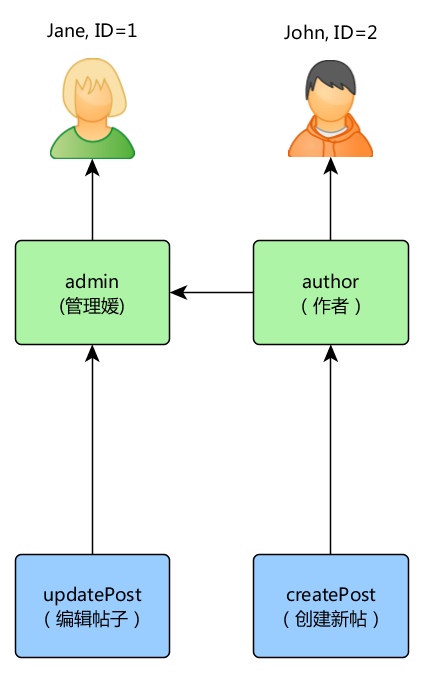
\includegraphics[width=\textwidth]{images/rbac-hierarchy-1.png}

Author can create post, admin can update post and do everything author can.

If your application allows user signup you need to assign roles to these new users once. For example, in order for all
signed up users to become authors you in advanced application template you need to modify \lstinline|frontend\models\SignupForm::signup()|
as follows:

\lstset{language=php}\begin{lstlisting}
public function signup()
{
    if ($this->validate()) {
        $user = new User();
        $user->username = $this->username;
        $user->email = $this->email;
        $user->setPassword($this->password);
        $user->generateAuthKey();
        $user->save(false);

        // the following three lines were added:
        $auth = Yii::$app->authManager;
        $authorRole = $auth->getRole('author');
        $auth->assign($authorRole, $user->getId());

        return $user;
    }

    return null;
}
\end{lstlisting}
For applications that require complex access control with dynamically updated authorization data, special user interfaces
(i.e. admin panel) may need to be developed using APIs offered by \lstinline|authManager|.

\begin{quote}Tip: By default, \texttt{yii{\allowbreak{}\textbackslash}rbac{\allowbreak{}\textbackslash}PhpManager} stores RBAC data in three files: \lstinline|@app/rbac/items.php|, \lstinline|@app/rbac/assignments.php| and \lstinline|@app/rbac/rules.php|.
  Make sure these files are writable by the Web server process if the authorization needs to be changed online.
  Sometimes you will need to create these files manually.

\end{quote}
\subsubsection{Using Rules}
As aforementioned, rules add additional constraint to roles and permissions. A rule is a class extending
from \texttt{yii{\allowbreak{}\textbackslash}rbac{\allowbreak{}\textbackslash}Rule}. It must implement the \texttt{yii{\allowbreak{}\textbackslash}rbac{\allowbreak{}\textbackslash}Rule\allowbreak{}::\allowbreak{}execute()} method. In the hierarchy we've
created previously author cannot edit his own post. Let's fix it. First we need a rule to verify that the user is the post author:

\lstset{language=php}\begin{lstlisting}
namespace app\rbac;

use yii\rbac\Rule;

/**
 * Checks if authorID matches user passed via params
 */
class AuthorRule extends Rule
{
    public $name = 'isAuthor';

    /**
     * @param string|integer $user the user ID.
     * @param Item $item the role or permission that this rule is associated with
     * @param array $params parameters passed to ManagerInterface::checkAccess().
     * @return boolean a value indicating whether the rule permits the role or permission it is associated with.
     */
    public function execute($user, $item, $params)
    {
        return isset($params['post']) ? $params['post']->createdBy == $user : false;
    }
}
\end{lstlisting}
The rule above checks if the \lstinline|post| is created by \lstinline|$user|. We'll create a special permission \lstinline|updateOwnPost| in the
command we've used previously:

\lstset{language=php}\begin{lstlisting}
$auth = Yii::$app->authManager;

// add the rule
$rule = new \app\rbac\AuthorRule;
$auth->add($rule);

// add the "updateOwnPost" permission and associate the rule with it.
$updateOwnPost = $auth->createPermission('updateOwnPost');
$updateOwnPost->description = 'Update own post';
$updateOwnPost->ruleName = $rule->name;
$auth->add($updateOwnPost);

// "updateOwnPost" will be used from "updatePost"
$auth->addChild($updateOwnPost, $updatePost);

// allow "author" to update their own posts
$auth->addChild($author, $updateOwnPost);
\end{lstlisting}
Now we've got the following hierarchy:

\noindent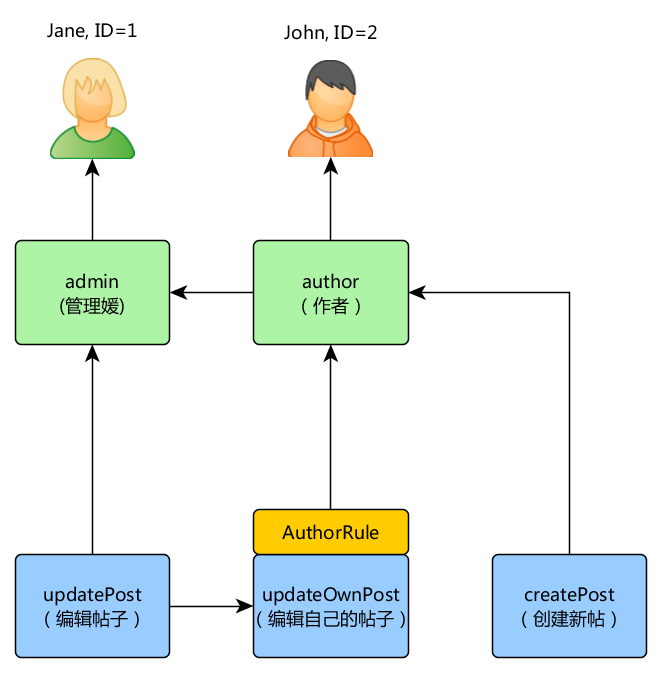
\includegraphics[width=\textwidth]{images/rbac-hierarchy-2.png}

\subsubsection{Access Check}
With the authorization data ready, access check is as simple as a call to the \texttt{yii{\allowbreak{}\textbackslash}rbac{\allowbreak{}\textbackslash}ManagerInterface\allowbreak{}::\allowbreak{}checkAccess()}
method. Because most access check is about the current user, for convenience Yii provides a shortcut method
\texttt{yii{\allowbreak{}\textbackslash}web{\allowbreak{}\textbackslash}User\allowbreak{}::\allowbreak{}can()}, which can be used like the following:

\lstset{language=php}\begin{lstlisting}
if (\Yii::$app->user->can('createPost')) {
    // create post
}
\end{lstlisting}
If the current user is Jane with ID=1 we're starting at \lstinline|createPost| and trying to get to \lstinline|Jane|:

\noindent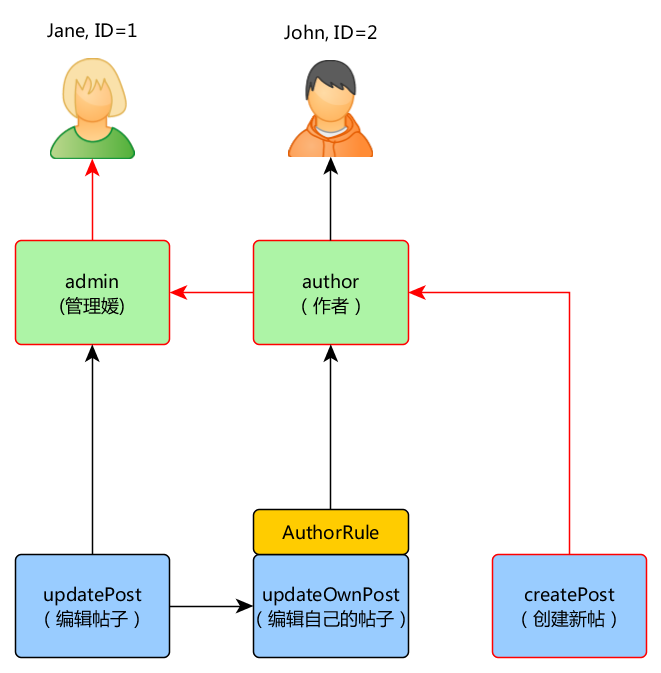
\includegraphics[width=\textwidth]{images/rbac-access-check-1.png}

In order to check if user can update post we need to pass an extra parameter that is required by the \lstinline|AuthorRule| described before:

\lstset{language=php}\begin{lstlisting}
if (\Yii::$app->user->can('updatePost', ['post' => $post])) {
    // update post
}
\end{lstlisting}
Here's what happens if current user is John:

\noindent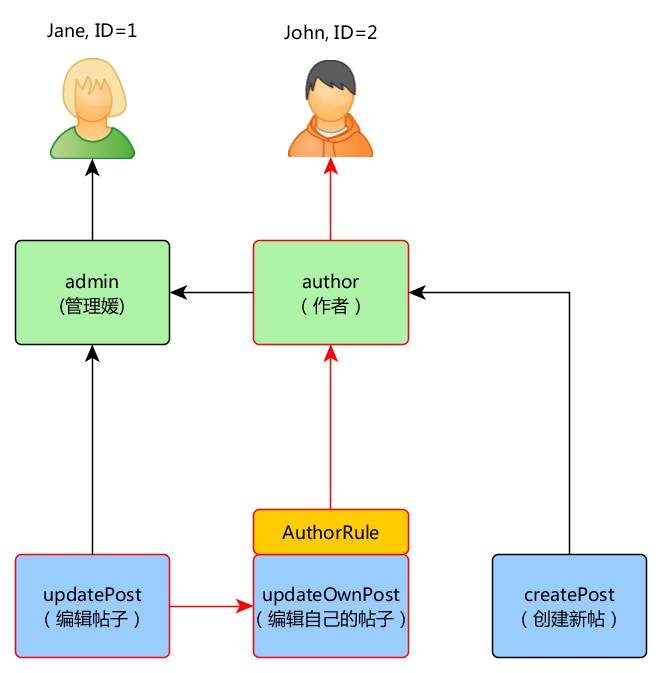
\includegraphics[width=\textwidth]{images/rbac-access-check-2.png}

We're starting with the \lstinline|updatePost| and going through \lstinline|updateOwnPost|. In order to pass it \lstinline|AuthorRule| should return
\lstinline|true| from its \lstinline|execute| method. The method receives its \lstinline|$params| from \lstinline|can| method call so the value is
\lstinline|['post' => $post]|. If everything is OK we're getting to \lstinline|author| that is assigned to John.

In case of Jane it is a bit simpler since she's an admin:

\noindent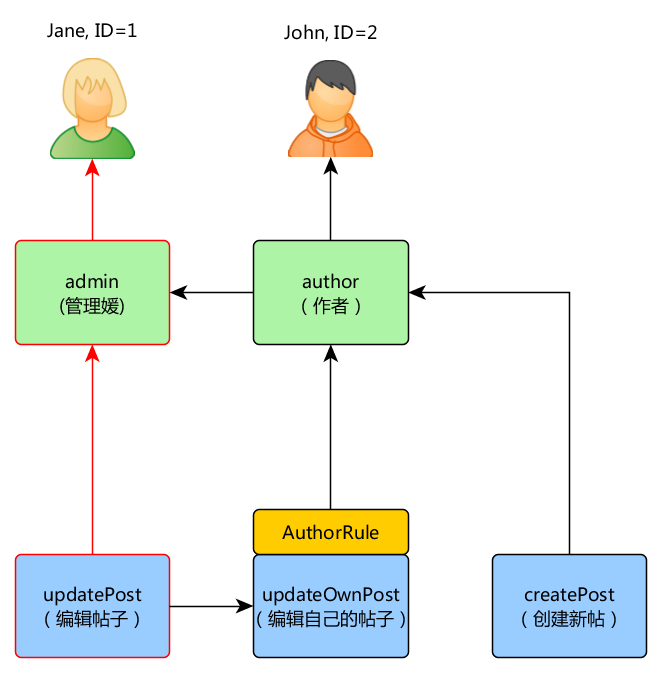
\includegraphics[width=\textwidth]{images/rbac-access-check-3.png}

\subsubsection{Using Default Roles}
A default role is a role that is \textit{implicitly} assigned to \textit{all} users. The call to \texttt{yii{\allowbreak{}\textbackslash}rbac{\allowbreak{}\textbackslash}ManagerInterface\allowbreak{}::\allowbreak{}assign()}
is not needed, and the authorization data does not contain its assignment information.

A default role is usually associated with a rule which determines if the role applies to the user being checked.

Default roles are often used in applications which already have some sort of role assignment. For example, an application
may have a ``group'' column in its user table to represent which privilege group each user belongs to.
If each privilege group can be mapped to a RBAC role, you can use the default role feature to automatically
assign each user to a RBAC role. Let's use an example to show how this can be done.

Assume in the user table, you have a \lstinline|group| column which uses 1 to represent the administrator group and 2 the author group.
You plan to have two RBAC roles \lstinline|admin| and \lstinline|author| to represent the permissions for these two groups, respectively.
You can create set up the RBAC data as follows,

\lstset{language=php}\begin{lstlisting}
namespace app\rbac;

use Yii;
use yii\rbac\Rule;

/**
 * Checks if user group matches
 */
class UserGroupRule extends Rule
{
    public $name = 'userGroup';

    public function execute($user, $item, $params)
    {
        if (!Yii::$app->user->isGuest) {
            $group = Yii::$app->user->identity->group;
            if ($item->name === 'admin') {
                return $group == 1;
            } elseif ($item->name === 'author') {
                return $group == 1 || $group == 2;
            }
        }
        return false;
    }
}

$auth = Yii::$app->authManager;

$rule = new \app\rbac\UserGroupRule;
$auth->add($rule);

$author = $auth->createRole('author');
$author->ruleName = $rule->name;
$auth->add($author);
// ... add permissions as children of $author ...

$admin = $auth->createRole('admin');
$admin->ruleName = $rule->name;
$auth->add($admin);
$auth->addChild($admin, $author);
// ... add permissions as children of $admin ...
\end{lstlisting}
Note that in the above, because ``author'' is added as a child of ``admin'', when you implement the \lstinline|execute()| method
of the rule class, you need to respect this hierarchy as well. That is why when the role name is ``author'',
the \lstinline|execute()| method will return true if the user group is either 1 or 2 (meaning the user is in either ``admin''
group or ``author'' group).

Next, configure \lstinline|authManager| by listing the two roles in \texttt{yii{\allowbreak{}\textbackslash}rbac{\allowbreak{}\textbackslash}BaseManager\allowbreak{}::\allowbreak{}\$defaultRoles}:

\lstset{language=php}\begin{lstlisting}
return [
    // ...
    'components' => [
        'authManager' => [
            'class' => 'yii\rbac\PhpManager',
            'defaultRoles' => ['admin', 'author'],
        ],
        // ...
    ],
];
\end{lstlisting}
Now if you perform an access check, both of the \lstinline|admin| and \lstinline|author| roles will be checked by evaluating
the rules associated with them. If the rule returns true, it means the role applies to the current user.
Based on the above rule implementation, this means if the \lstinline|group| value of a user is 1, the \lstinline|admin| role
would apply to the user; and if the \lstinline|group| value is 2, the \lstinline|author| role would apply.



\label{security-passwords.md}\section{Security}
\begin{quote}Note: This section is under development.

\end{quote}
Good security is vital to the health and success of any application. Unfortunately, many developers cut corners when it comes to security, either due to a lack of understanding or because implementation is too much of a hurdle. To make your Yii powered application as secure as possible, Yii has included several excellent and easy to use security features.

\subsection{Hashing and verifying passwords}
Most developers know that passwords cannot be stored in plain text, but many developers believe it's still safe to hash passwords using \lstinline|md5| or \lstinline|sha1|. There was a time when using the aforementioned hashing algorithms was sufficient, but modern hardware makes it possible to reverse such hashes very quickly using brute force attacks.

In order to provide increased security for user passwords, even in the worst case scenario (your application is breached), you need to use a hashing algorithm that is resilient against brute force attacks. The best current choice is \lstinline|bcrypt|. In PHP, you can create a \lstinline|bcrypt| hash  using the crypt function\footnote{\url{http://php.net/manual/en/function.crypt.php}}. Yii provides two helper functions which make using \lstinline|crypt| to securely generate and verify hashes easier.

When a user provides a password for the first time (e.g., upon registration), the password needs to be hashed:

\lstset{language=php}\begin{lstlisting}
$hash = Yii::$app->getSecurity()->generatePasswordHash($password);
\end{lstlisting}
The hash can then be associated with the corresponding model attribute, so it can be stored in the database for later use.

When a user attempts to log in, the submitted password must be verified against the previously hashed and stored password:

\lstset{language=php}\begin{lstlisting}
if (Yii::$app->getSecurity()->validatePassword($password, $hash)) {
    // all good, logging user in
} else {
    // wrong password
}
\end{lstlisting}
\subsection{Generating Pseudorandom data}
Pseudorandom data is useful in many situations. For example when resetting a password via email you need to generate a token, save it to the database, and send it via email to end user which in turn will allow them to prove ownership of that account. It is very important that this token be unique and hard to guess, else there is a possibility that attacker can predict the token's value and reset the user's password.

Yii security helper makes generating pseudorandom data simple:

\lstset{language=php}\begin{lstlisting}
$key = Yii::$app->getSecurity()->generateRandomString();
\end{lstlisting}
Note that you need to have the \lstinline|openssl| extension installed in order to generate cryptographically secure random data.

\subsection{Encryption and decryption}
Yii provides convenient helper functions that allow you to encrypt/decrypt data using a secret key. The data is passed through the encryption function so that only the person which has the secret key will be able to decrypt it.
For example, we need to store some information in our database but we need to make sure only the user which has the secret key can view it (even if the application database is compromised):

\lstset{language=php}\begin{lstlisting}
// $data and $secretKey are obtained from the form
$encryptedData = Yii::$app->getSecurity()->encrypt($data, $secretKey);
// store $encryptedData to database
\end{lstlisting}
Subsequently when user wants to read the data:

\lstset{language=php}\begin{lstlisting}
// $secretKey is obtained from user input, $encryptedData is from the database
$data = Yii::$app->getSecurity()->decrypt($encryptedData, $secretKey);
\end{lstlisting}
\subsection{Confirming data integrity}
There are situations in which you need to verify that your data hasn't been tampered with by a third party or even corrupted in some way. Yii provides an easy way to confirm data integrity in the form of two helper functions.

Prefix the data with a hash generated from the secret key and data

\lstset{language=php}\begin{lstlisting}
// $secretKey our application or user secret, $genuineData obtained from a reliable source
$data = Yii::$app->getSecurity()->hashData($genuineData, $secretKey);
\end{lstlisting}
Checks if the data integrity has been compromised

\lstset{language=php}\begin{lstlisting}
// $secretKey our application or user secret, $data obtained from an unreliable source
$data = Yii::$app->getSecurity()->validateData($data, $secretKey);
\end{lstlisting}
todo: XSS prevention, CSRF prevention, cookie protection, refer to 1.1 guide

You also can disable CSRF validation per controller and/or action, by setting its property:

\lstset{language=php}\begin{lstlisting}
namespace app\controllers;

use yii\web\Controller;

class SiteController extends Controller
{
    public $enableCsrfValidation = false;

    public function actionIndex()
    {
        // CSRF validation will not be applied to this and other actions
    }

}
\end{lstlisting}
To disable CSRF validation per custom actions you can do:

\lstset{language=php}\begin{lstlisting}
namespace app\controllers;

use yii\web\Controller;

class SiteController extends Controller
{
    public function beforeAction($action)
    {
        // ...set `$this->enableCsrfValidation` here based on some conditions...
        // call parent method that will check CSRF if such property is true.
        return parent::beforeAction($action);
    }
}
\end{lstlisting}
\subsection{Securing Cookies}
\begin{itemize}
\item validation
\item httpOnly is default
\end{itemize}
\subsection{See also}
\begin{itemize}
\item \hyperref[structure-views.md::security]{Views security}
\end{itemize}


\label{security-auth-clients.md}\section{Auth Clients}
\begin{quote}Note: This section is under development.

It has no content yet.

\end{quote}


\label{security-best-practices.md}\section{Security best practice}
\begin{quote}Note: This section is under development.

It has no content yet.

\end{quote}


\chapter{缓存}
\label{caching-overview.md}\section{缓存}
缓存是提升 Web 应用性能简便有效的方式。通过将相对静态的数据存储到缓存并在收到请求时取回缓存,应用程序便节省了每次重新生成这些数据所需的时间。

缓存可以应用在 Web 应用程序的任何层级任何位置。在服务器端,在较的低层面,缓存可能用于存储基础数据,例如从数据库中取出的最新文章列表;在较高的层面,缓存可能用于存储一段或整个 Web 页面,例如最新文章的渲染结果。在客户端,HTTP 缓存可能用于将最近访问的页面内容存储到浏览器缓存中。

Yii 支持如上所有缓存机制:

\begin{itemize}
\item \hyperref[caching-data.md]{数据缓存}
\item \hyperref[caching-fragment.md]{片段缓存}
\item \hyperref[caching-page.md]{页面缓存}
\item \hyperref[caching-http.md]{HTTP 缓存}
\end{itemize}


\label{caching-data.md}\section{数据缓存}
数据缓存是指将一些 PHP 变量存储到缓存中,使用时再从缓存中取回。它也是更高级缓存特性的基础,例如\hyperref[caching-data.md::::query-caching]{查询缓存}和\hyperref[caching-content.md]{内容缓存}。

如下代码是一个典型的数据缓存使用模式。其中 \lstinline|$cache| 指向\hyperref[caching-data.md::::cache-components]{缓存组件}:

\lstset{language=php}\begin{lstlisting}
// 尝试从缓存中取回 $data 
$data = $cache->get($key);

if ($data === false) {

    // $data 在缓存中没有找到,则重新计算它的值

    // 将 $data 存放到缓存供下次使用
    $cache->set($key, $data);
}

// 这儿 $data 可以使用了。
\end{lstlisting}
\subsection{缓存组件 \label{caching-data.md::cache-components}}
数据缓存需要\textbf{缓存组件}提供支持,它代表各种缓存存储器,例如内存,文件,数据库。

缓存组件通常注册为应用程序组件,这样它们就可以在全局进行配置与访问。如下代码演示了如何配置应用程序组件 \lstinline|cache| 使用两个 memcached\footnote{\url{http://memcached.org/}} 服务器:

\lstset{language=php}\begin{lstlisting}
'components' => [
    'cache' => [
        'class' => 'yii\caching\MemCache',
        'servers' => [
            [
                'host' => 'server1',
                'port' => 11211,
                'weight' => 100,
            ],
            [
                'host' => 'server2',
                'port' => 11211,
                'weight' => 50,
            ],
        ],
    ],
],
\end{lstlisting}
然后就可以通过  \lstinline|Yii::$app->cache| 访问上面的缓存组件了。

由于所有缓存组件都支持同样的一系列 API ,并不需要修改使用缓存的业务代码就能直接替换为其他底层缓存组件,只需在应用配置中重新配置一下就可以。例如,你可以将上述配置修改为使用 \texttt{yii{\allowbreak{}\textbackslash}caching{\allowbreak{}\textbackslash}ApcCache}:

\lstset{language=php}\begin{lstlisting}
'components' => [
    'cache' => [
        'class' => 'yii\caching\ApcCache',
    ],
],
\end{lstlisting}
\begin{quote}Tip: 你可以注册多个缓存组件,很多依赖缓存的类默认调用名为 \lstinline|cache| 的组件(例如 \texttt{yii{\allowbreak{}\textbackslash}web{\allowbreak{}\textbackslash}UrlManager})。

\end{quote}
\subsubsection{支持的缓存存储器 \label{caching-data.md::supported-cache-storage}}
Yii 支持一系列缓存存储器,概况如下:

\begin{itemize}
\item \texttt{yii{\allowbreak{}\textbackslash}caching{\allowbreak{}\textbackslash}ApcCache}:使用 PHP APC\footnote{\url{http://php.net/manual/en/book.apc.php}} 扩展。这个选项可以认为是集中式应用程序环境中(例如:单一服务器,没有独立的负载均衡器等)最快的缓存方案。
\item \texttt{yii{\allowbreak{}\textbackslash}caching{\allowbreak{}\textbackslash}DbCache}:使用一个数据库的表存储缓存数据。要使用这个缓存,你必须创建一个与 \texttt{yii{\allowbreak{}\textbackslash}caching{\allowbreak{}\textbackslash}DbCache\allowbreak{}::\allowbreak{}cacheTable} 对应的表。
\item \texttt{yii{\allowbreak{}\textbackslash}caching{\allowbreak{}\textbackslash}DummyCache}: 仅作为一个缓存占位符,不实现任何真正的缓存功能。这个组件的目的是为了简化那些需要查询缓存有效性的代码。例如,在开发中如果服务器没有实际的缓存支持,用它配置一个缓存组件。一个真正的缓存服务启用后,可以再切换为使用相应的缓存组件。两种条件下你都可以使用同样的代码 \lstinline|Yii::$app->cache->get($key)| 尝试从缓存中取回数据而不用担心 \lstinline|Yii::$app->cache| 可能是 \lstinline|null|。
\item \texttt{yii{\allowbreak{}\textbackslash}caching{\allowbreak{}\textbackslash}FileCache}:使用标准文件存储缓存数据。这个特别适用于缓存大块数据,例如一个整页的内容。
\item \texttt{yii{\allowbreak{}\textbackslash}caching{\allowbreak{}\textbackslash}MemCache}:使用 PHP memcache\footnote{\url{http://php.net/manual/en/book.memcache.php}} 和 memcached\footnote{\url{http://php.net/manual/en/book.memcached.php}} 扩展。这个选项被看作分布式应用环境中(例如:多台服务器,有负载均衡等)最快的缓存方案。
\item \texttt{yii{\allowbreak{}\textbackslash}redis{\allowbreak{}\textbackslash}Cache}:实现了一个基于 Redis\footnote{\url{http://redis.io/}} 键值对存储器的缓存组件(需要 redis 2.6.12 及以上版本的支持 )。
\item \texttt{yii{\allowbreak{}\textbackslash}caching{\allowbreak{}\textbackslash}WinCache}:使用 PHP WinCache\footnote{\url{http://iis.net/downloads/microsoft/wincache-extension}}(另可参考\footnote{\url{http://php.net/manual/en/book.wincache.php}})扩展.
\item \texttt{yii{\allowbreak{}\textbackslash}caching{\allowbreak{}\textbackslash}XCache}:使用 PHP XCache\footnote{\url{http://xcache.lighttpd.net/}}扩展。
\item \texttt{yii{\allowbreak{}\textbackslash}caching{\allowbreak{}\textbackslash}ZendDataCache}:使用 Zend Data Cache\footnote{\url{http://files.zend.com/help/Zend-Server-6/zend-server.htm\#data\_cache\_component.htm}} 作为底层缓存媒介。
\end{itemize}
\begin{quote}Tip: 你可以在同一个应用程序中使用不同的缓存存储器。一个常见的策略是使用基于内存的缓存存储器存储小而常用的数据(例如:统计数据),使用基于文件或数据库的缓存存储器存储大而不太常用的数据(例如:网页内容)。

\end{quote}
\subsection{缓存 API \label{caching-data.md::cache-apis}}
所有缓存组件都有同样的基类 \texttt{yii{\allowbreak{}\textbackslash}caching{\allowbreak{}\textbackslash}Cache} ,因此都支持如下 API:

\begin{itemize}
\item \texttt{yii{\allowbreak{}\textbackslash}caching{\allowbreak{}\textbackslash}Cache\allowbreak{}::\allowbreak{}get()}:通过一个指定的键(key)从缓存中取回一项数据。如果该项数据不存在于缓存中或者已经过期/失效,则返回值 false。
\item \texttt{yii{\allowbreak{}\textbackslash}caching{\allowbreak{}\textbackslash}Cache\allowbreak{}::\allowbreak{}set()}:将一项数据指定一个键,存放到缓存中。
\item \texttt{yii{\allowbreak{}\textbackslash}caching{\allowbreak{}\textbackslash}Cache\allowbreak{}::\allowbreak{}add()}:如果缓存中未找到该键,则将指定数据存放到缓存中。
\item \texttt{yii{\allowbreak{}\textbackslash}caching{\allowbreak{}\textbackslash}Cache\allowbreak{}::\allowbreak{}mget()}:通过指定的多个键从缓存中取回多项数据。
\item \texttt{yii{\allowbreak{}\textbackslash}caching{\allowbreak{}\textbackslash}Cache\allowbreak{}::\allowbreak{}mset()}:将多项数据存储到缓存中,每项数据对应一个键。
\item \texttt{yii{\allowbreak{}\textbackslash}caching{\allowbreak{}\textbackslash}Cache\allowbreak{}::\allowbreak{}madd()}:将多项数据存储到缓存中,每项数据对应一个键。如果某个键已经存在于缓存中,则该项数据会被跳过。
\item \texttt{yii{\allowbreak{}\textbackslash}caching{\allowbreak{}\textbackslash}Cache\allowbreak{}::\allowbreak{}exists()}:返回一个值,指明某个键是否存在于缓存中。
\item \texttt{yii{\allowbreak{}\textbackslash}caching{\allowbreak{}\textbackslash}Cache\allowbreak{}::\allowbreak{}delete()}:通过一个键,删除缓存中对应的值。
\item \texttt{yii{\allowbreak{}\textbackslash}caching{\allowbreak{}\textbackslash}Cache\allowbreak{}::\allowbreak{}flush()}:删除缓存中的所有数据。
\end{itemize}
有些缓存存储器如 MemCache,APC 支持以批量模式取回缓存值,这样可以节省取回缓存数据的开支。 \texttt{yii{\allowbreak{}\textbackslash}caching{\allowbreak{}\textbackslash}Cache\allowbreak{}::\allowbreak{}mget()} 和 \texttt{yii{\allowbreak{}\textbackslash}caching{\allowbreak{}\textbackslash}Cache\allowbreak{}::\allowbreak{}madd()} API提供对该特性的支持。如果底层缓存存储器不支持该特性,Yii 也会模拟实现。

由于 \texttt{yii{\allowbreak{}\textbackslash}caching{\allowbreak{}\textbackslash}Cache} 实现了 PHP \lstinline|ArrayAccess| 接口,缓存组件也可以像数组那样使用,下面是几个例子:

\lstset{language=php}\begin{lstlisting}
$cache['var1'] = $value1;  // 等价于: $cache->set('var1', $value1);
$value2 = $cache['var2'];  // 等价于: $value2 = $cache->get('var2');
\end{lstlisting}
\subsubsection{缓存键 \label{caching-data.md::cache-keys}}
存储在缓存中的每项数据都通过键作唯一识别。当你在缓存中存储一项数据时,必须为它指定一个键,稍后从缓存中取回数据时,也需要提供相应的键。

你可以使用一个字符串或者任意值作为一个缓存键。当键不是一个字符串时,它将会自动被序列化为一个字符串。

定义一个缓存键常见的一个策略就是在一个数组中包含所有的决定性因素。例如,\texttt{yii{\allowbreak{}\textbackslash}db{\allowbreak{}\textbackslash}Schema} 使用如下键存储一个数据表的结构信息。

\lstset{language=php}\begin{lstlisting}
[
    __CLASS__,              // 结构类名
    $this->db->dsn,         // 数据源名称
    $this->db->username,    // 数据库登录用户名
    $name,                  // 表名
];
\end{lstlisting}
如你所见,该键包含了可唯一指定一个数据库表所需的所有必要信息。

当同一个缓存存储器被用于多个不同的应用时,应该为每个应用指定一个唯一的缓存键前缀以避免缓存键冲突。可以通过配置 \texttt{yii{\allowbreak{}\textbackslash}caching{\allowbreak{}\textbackslash}Cache\allowbreak{}::\allowbreak{}keyPrefix} 属性实现。例如,在应用配置中可以编写如下代码:

\lstset{language=php}\begin{lstlisting}
'components' => [
    'cache' => [
        'class' => 'yii\caching\ApcCache',
        'keyPrefix' => 'myapp',       // 唯一键前缀
    ],
],
\end{lstlisting}
为了确保互通性,此处只能使用字母和数字。

\subsubsection{缓存过期 \label{caching-data.md::cache-expiration}}
默认情况下,缓存中的数据会永久存留,除非它被某些缓存策略强制移除(例如:缓存空间已满,最老的数据会被移除)。要改变此特性,你可以在调用 \texttt{yii{\allowbreak{}\textbackslash}caching{\allowbreak{}\textbackslash}Cache\allowbreak{}::\allowbreak{}set()} 存储一项数据时提供一个过期时间参数。该参数代表这项数据在缓存中可保持有效多少秒。当你调用 \texttt{yii{\allowbreak{}\textbackslash}caching{\allowbreak{}\textbackslash}Cache\allowbreak{}::\allowbreak{}get()} 取回数据时,如果它已经过了超时时间,该方法将返回 false,表明在缓存中找不到这项数据。例如:

\lstset{language=php}\begin{lstlisting}
// 将数据在缓存中保留 45 秒
$cache->set($key, $data, 45);

sleep(50);

$data = $cache->get($key);
if ($data === false) {
    // $data 已过期,或者在缓存中找不到
}
\end{lstlisting}
\subsubsection{缓存依赖 \label{caching-data.md::cache-dependencies}}
除了超时设置,缓存数据还可能受到\textbf{缓存依赖}的影响而失效。例如,\texttt{yii{\allowbreak{}\textbackslash}caching{\allowbreak{}\textbackslash}FileDependency} 代表对一个文件修改时间的依赖。这个依赖条件发生变化也就意味着相应的文件已经被修改。因此,缓存中任何过期的文件内容都应该被置为失效状态,对 \texttt{yii{\allowbreak{}\textbackslash}caching{\allowbreak{}\textbackslash}Cache\allowbreak{}::\allowbreak{}get()} 的调用都应该返回 false。

缓存依赖用 \texttt{yii{\allowbreak{}\textbackslash}caching{\allowbreak{}\textbackslash}Dependency} 的派生类所表示。当调用 \texttt{yii{\allowbreak{}\textbackslash}caching{\allowbreak{}\textbackslash}Cache\allowbreak{}::\allowbreak{}set()} 在缓存中存储一项数据时,可以同时传递一个关联的缓存依赖对象。例如:

\lstset{language=php}\begin{lstlisting}
// 创建一个对 example.txt 文件修改时间的缓存依赖
$dependency = new \yii\caching\FileDependency(['fileName' => 'example.txt']);

// 缓存数据将在30秒后超时
// 如果 example.txt 被修改,它也可能被更早地置为失效状态。
$cache->set($key, $data, 30, $dependency);

// 缓存会检查数据是否已超时。
// 它还会检查关联的依赖是否已变化。
// 符合任何一个条件时都会返回 false。
$data = $cache->get($key);
\end{lstlisting}
下面是可用的缓存依赖的概况:

\begin{itemize}
\item \texttt{yii{\allowbreak{}\textbackslash}caching{\allowbreak{}\textbackslash}ChainedDependency}:如果依赖链上任何一个依赖产生变化,则依赖改变。
\item \texttt{yii{\allowbreak{}\textbackslash}caching{\allowbreak{}\textbackslash}DbDependency}:如果指定 SQL 语句的查询结果发生了变化,则依赖改变。
\item \texttt{yii{\allowbreak{}\textbackslash}caching{\allowbreak{}\textbackslash}ExpressionDependency}:如果指定的 PHP 表达式执行结果发生变化,则依赖改变。
\item \texttt{yii{\allowbreak{}\textbackslash}caching{\allowbreak{}\textbackslash}FileDependency}:如果文件的最后修改时间发生变化,则依赖改变。
\item \texttt{yii{\allowbreak{}\textbackslash}caching{\allowbreak{}\textbackslash}GroupDependency}:将一项缓存数据标记到一个组名,你可以通过调用 \texttt{yii{\allowbreak{}\textbackslash}caching{\allowbreak{}\textbackslash}GroupDependency\allowbreak{}::\allowbreak{}invalidate()} 一次性将相同组名的缓存全部置为失效状态。
\end{itemize}
\subsection{查询缓存 \label{caching-data.md::query-caching}}
查询缓存是一个建立在数据缓存之上的特殊缓存特性。它用于缓存数据库查询的结果。

查询缓存需要一个 \texttt{yii{\allowbreak{}\textbackslash}db{\allowbreak{}\textbackslash}Connection} 和一个有效的 \lstinline|cache| 应用组件。查询缓存的基本用法如下,假设 \lstinline|$db| 是一个 \texttt{yii{\allowbreak{}\textbackslash}db{\allowbreak{}\textbackslash}Connection} 实例:

\lstset{language=php}\begin{lstlisting}
$duration = 60;     // 缓存查询结果60秒
$dependency = ...;  // 可选的缓存依赖

$db->beginCache($duration, $dependency);

// ...这儿执行数据库查询...

$db->endCache();
\end{lstlisting}
如你所见,\lstinline|beginCache()| 和 \lstinline|endCache()| 中间的任何查询结果都会被缓存起来。如果缓存中找到了同样查询的结果,则查询会被跳过,直接从缓存中提取结果。

查询缓存可以用于 \hyperref[db-active-record.md]{ActiveRecord} 和 \hyperref[db-dao.md]{DAO}。

\begin{quote}Info: 有些 DBMS (例如:MySQL\footnote{\url{http://dev.mysql.com/doc/refman/5.1/en/query-cache.html}})也支持数据库服务器端的查询缓存。你可以选择使用任一查询缓存机制。上文所述的查询缓存的好处在于你可以指定更灵活的缓存依赖因此可能更加高效。

\end{quote}
\subsubsection{配置 \label{caching-data.md::query-caching-configs}}
查询缓存有两个通过 \texttt{yii{\allowbreak{}\textbackslash}db{\allowbreak{}\textbackslash}Connection} 设置的配置项:

\begin{itemize}
\item \texttt{yii{\allowbreak{}\textbackslash}db{\allowbreak{}\textbackslash}Connection\allowbreak{}::\allowbreak{}queryCacheDuration}: 查询结果在缓存中的有效期,以秒表示。如果在调用 \texttt{yii{\allowbreak{}\textbackslash}db{\allowbreak{}\textbackslash}Connection\allowbreak{}::\allowbreak{}beginCache()} 时传递了一个显式的时值参数,则配置中的有效期时值会被覆盖。
\item \texttt{yii{\allowbreak{}\textbackslash}db{\allowbreak{}\textbackslash}Connection\allowbreak{}::\allowbreak{}queryCache}: 缓存应用组件的 ID。默认为 \lstinline|'cache'|。只有在设置了一个有效的缓存应用组件时,查询缓存才会有效。
\end{itemize}
\subsubsection{限制条件 \label{caching-data.md::query-caching-limitations}}
当查询结果中含有资源句柄时,查询缓存无法使用。例如,在有些 DBMS 中使用了 \lstinline|BLOB| 列的时候,缓存结果会为该数据列返回一个资源句柄。

有些缓存存储器有大小限制。例如,memcache 限制每条数据最大为 1MB。因此,如果查询结果的大小超出了该限制,则会导致缓存失败。



\label{caching-fragment.md}\section{片段缓存}
片段缓存指的是缓存页面内容中的某个片段。例如,一个页面显示了逐年销售额的摘要表格,可以把表格缓存下来,以消除每次请求都要重新生成表格的耗时。片段缓存是基于\hyperref[caching-data.md]{数据缓存}实现的。

在\hyperref[structure-views.md]{视图}中使用以下结构启用片段缓存:

\lstset{language=php}\begin{lstlisting}
if ($this->beginCache($id)) {

    // ... 在此生成内容 ...

    $this->endCache();
}
\end{lstlisting}
调用 \texttt{yii{\allowbreak{}\textbackslash}base{\allowbreak{}\textbackslash}View\allowbreak{}::\allowbreak{}beginCache()} 和 \texttt{yii{\allowbreak{}\textbackslash}base{\allowbreak{}\textbackslash}View\allowbreak{}::\allowbreak{}endCache()} 方法包裹内容生成逻辑。如果缓存中存在该内容,\texttt{yii{\allowbreak{}\textbackslash}base{\allowbreak{}\textbackslash}View\allowbreak{}::\allowbreak{}beginCache()} 方法将渲染内容并返回 false,因此将跳过内容生成逻辑。否则,内容生成逻辑被执行,一直执行到 \texttt{yii{\allowbreak{}\textbackslash}base{\allowbreak{}\textbackslash}View\allowbreak{}::\allowbreak{}endCache()} 时,生成的内容将被捕获并存储在缓存中。

和[[数据缓存]](caching-data.md)一样,每个片段缓存也需要全局唯一的 \lstinline|$id| 标记。

\subsection{缓存选项 \label{caching-fragment.md::caching-options}}
如果要为片段缓存指定额外配置项,请通过向 \texttt{yii{\allowbreak{}\textbackslash}base{\allowbreak{}\textbackslash}View\allowbreak{}::\allowbreak{}beginCache()} 方法第二个参数传递配置数组。在框架内部,该数组将被用来配置一个 \texttt{yii{\allowbreak{}\textbackslash}widget{\allowbreak{}\textbackslash}FragmentCache} 小部件用以实现片段缓存功能。

\subsubsection{过期时间(duration) \label{caching-fragment.md::duration}}
或许片段缓存中最常用的一个配置选项就是 \texttt{yii{\allowbreak{}\textbackslash}widgets{\allowbreak{}\textbackslash}FragmentCache\allowbreak{}::\allowbreak{}duration} 了。它指定了内容被缓存的秒数。以下代码缓存内容最多一小时:

\lstset{language=php}\begin{lstlisting}
if ($this->beginCache($id, ['duration' => 3600])) {

    // ... 在此生成内容 ...

    $this->endCache();
}
\end{lstlisting}
如果该选项未设置,则默认为 0,永不过期。

\subsubsection{依赖 \label{caching-fragment.md::dependencies}}
和[[数据缓存]](caching-data.md)一样,片段缓存的内容一样可以设置缓存依赖。例如一段被缓存的文章,是否重新缓存取决于它是否被修改过。

通过设置 \texttt{yii{\allowbreak{}\textbackslash}widgets{\allowbreak{}\textbackslash}FragmentCache\allowbreak{}::\allowbreak{}dependency} 选项来指定依赖,该选项的值可以是一个 \texttt{yii{\allowbreak{}\textbackslash}caching{\allowbreak{}\textbackslash}Dependency} 类的派生类,也可以是创建缓存对象的配置数组。以下代码指定了一个片段缓存,它依赖于 \lstinline|update_at| 字段是否被更改过的。

\lstset{language=php}\begin{lstlisting}
$dependency = [
    'class' => 'yii\caching\DbDependency',
    'sql' => 'SELECT MAX(updated_at) FROM post',
];

if ($this->beginCache($id, ['dependency' => $dependency])) {

    // ... 在此生成内容 ...

    $this->endCache();
}
\end{lstlisting}
\subsubsection{变化 \label{caching-fragment.md::variations}}
缓存的内容可能需要根据一些参数的更改而变化。例如一个 Web 应用支持多语言,同一段视图代码也许需要生成多个语言的内容。因此可以设置缓存根据应用当前语言而变化。

通过设置 \texttt{yii{\allowbreak{}\textbackslash}widgets{\allowbreak{}\textbackslash}FragmentCache\allowbreak{}::\allowbreak{}variations} 选项来指定变化,该选项的值应该是一个标量,每个标量代表不同的变化系数。例如设置缓存根据当前语言而变化可以用以下代码:

\lstset{language=php}\begin{lstlisting}
if ($this->beginCache($id, ['variations' => [Yii::$app->language]])) {

    // ... 在此生成内容 ...

    $this->endCache();
}
\end{lstlisting}
\subsubsection{开关 \label{caching-fragment.md::toggling-caching}}
有时你可能只想在特定条件下开启片段缓存。例如,一个显示表单的页面,可能只需要在初次请求时缓存表单(通过 GET 请求)。随后请求所显示(通过 POST 请求)的表单不该使用缓存,因为此时表单中可能包含用户输入内容。鉴于此种情况,可以使用 \texttt{yii{\allowbreak{}\textbackslash}widgets{\allowbreak{}\textbackslash}FragmentCache\allowbreak{}::\allowbreak{}enabled} 选项来指定缓存开关,如下所示:

\lstset{language=php}\begin{lstlisting}
if ($this->beginCache($id, ['enabled' => Yii::$app->request->isGet])) {

    // ... 在此生成内容 ...

    $this->endCache();
}
\end{lstlisting}
\subsection{缓存嵌套 \label{caching-fragment.md::nested-caching}}
片段缓存可以被嵌套使用。一个片段缓存可以被另一个包裹。例如,评论被缓存在里层,同时整个评论的片段又被缓存在外层的文章中。以下代码展示了片段缓存的嵌套使用:

\lstset{language=php}\begin{lstlisting}
if ($this->beginCache($id1)) {

    // ...在此生成内容...

    if ($this->beginCache($id2, $options2)) {

        // ...在此生成内容...

        $this->endCache();
    }

    // ...在此生成内容...

    $this->endCache();
}
\end{lstlisting}
可以为嵌套的缓存设置不同的配置项。例如,内层缓存和外层缓存使用不同的过期时间。甚至当外层缓存的数据过期失效了,内层缓存仍然可能提供有效的片段缓存数据。但是,反之则不然。如果外层片段缓存没有过期而被视为有效,此时即使内层片段缓存已经失效,它也将继续提供同样的缓存副本。因此,你必须谨慎处理缓存嵌套中的过期时间和依赖,否则外层的片段很有可能返回的是不符合你预期的失效数据。

\begin{quote}译者注:外层的失效时间应该短于内层,外层的依赖条件应该低于内层,以确保最小的片段,返回的是最新的数据。

\end{quote}
\subsection{动态内容 \label{caching-fragment.md::dynamic-content}}
使用片段缓存时,可能会遇到一大段较为静态的内容中有少许动态内容的情况。例如,一个显示着菜单栏和当前用户名的页面头部。还有一种可能是缓存的内容可能包含每次请求都需要执行的 PHP 代码(例如注册资源包的代码)。这两个问题都可以使用\textbf{动态内容}功能解决。

动态内容的意思是这部分输出的内容不该被缓存,即便是它被包裹在片段缓存中。为了使内容保持动态,每次请求都执行 PHP 代码生成,即使这些代码已经被缓存了。

可以在片段缓存中调用 \texttt{yii{\allowbreak{}\textbackslash}base{\allowbreak{}\textbackslash}View\allowbreak{}::\allowbreak{}renderDynamic()} 去插入动态内容,如下所示:

\lstset{language=php}\begin{lstlisting}
if ($this->beginCache($id1)) {

    // ...在此生成内容...

    echo $this->renderDynamic('return Yii::$app->user->identity->name;');

    // ...在此生成内容...

    $this->endCache();
}
\end{lstlisting}
\texttt{yii{\allowbreak{}\textbackslash}base{\allowbreak{}\textbackslash}View\allowbreak{}::\allowbreak{}renderDynamic()} 方法接受一段 PHP 代码作为参数。代码的返回值被看作是动态内容。这段代码将在每次请求时都执行,无论其外层的片段缓存是否被存储。



\label{caching-page.md}\section{页面缓存}
页面缓存指的是在服务器端缓存整个页面的内容。随后当同一个页面被请求时,内容将从缓存中取出,而不是重新生成。

页面缓存由 \texttt{yii{\allowbreak{}\textbackslash}filters{\allowbreak{}\textbackslash}PageCache} 类提供支持,该类是一个\hyperref[structure-filters.md]{过滤器}。它可以像这样在控制器类中使用:

\lstset{language=php}\begin{lstlisting}
public function behaviors()
{
    return [
        [
            'class' => 'yii\filters\PageCache',
            'only' => ['index'],
            'duration' => 60,
            'variations' => [
                \Yii::$app->language,
            ],
            'dependency' => [
                'class' => 'yii\caching\DbDependency',
                'sql' => 'SELECT COUNT(*) FROM post',
            ],
        ],
    ];
}
\end{lstlisting}
上述代码表示页面缓存只在 \lstinline|index| 操作时启用,页面内容最多被缓存 60 秒,会随着当前应用的语言更改而变化。如果文章总数发生变化则缓存的页面会失效。

如你所见,页面缓存和\hyperref[caching-fragment.md]{片段缓存}极其相似。它们都支持 \lstinline|duration|,\lstinline|dependencies|,\lstinline|variations| 和 \lstinline|enabled| 配置选项。它们的主要区别是页面缓存是由\hyperref[structure-filters.md]{过滤器}实现,而片段缓存则是一个\hyperref[structure-widgets.md]{小部件}。

你可以在使用页面缓存的同时,使用\hyperref[caching-fragment.md]{片段缓存}和\hyperref[caching-fragment.md::dynamic-content]{动态内容}。



\label{caching-http.md}\section{HTTP 缓存}
除了前面章节讲到的服务器端缓存外, Web 应用还可以利用客户端缓存去节省相同页面内容的生成和传输时间。

通过配置 \texttt{yii{\allowbreak{}\textbackslash}filters{\allowbreak{}\textbackslash}HttpCache} 过滤器,控制器操作渲染的内容就能缓存在客户端。\texttt{yii{\allowbreak{}\textbackslash}filters{\allowbreak{}\textbackslash}HttpCache} 过滤器仅对 \lstinline|GET| 和 \lstinline|HEAD| 请求生效,它能为这些请求设置三种与缓存有关的 HTTP 头。

\begin{itemize}
\item \texttt{yii{\allowbreak{}\textbackslash}filters{\allowbreak{}\textbackslash}HttpCache\allowbreak{}::\allowbreak{}lastModified}
\item \texttt{yii{\allowbreak{}\textbackslash}filters{\allowbreak{}\textbackslash}HttpCache\allowbreak{}::\allowbreak{}etagSeed}
\item \texttt{yii{\allowbreak{}\textbackslash}filters{\allowbreak{}\textbackslash}HttpCache\allowbreak{}::\allowbreak{}cacheControlHeader}
\end{itemize}
\subsection{\lstinline|Last-Modified| 头 \label{caching-http.md::last-modified}}
\lstinline|Last-Modified| 头使用时间戳标明页面自上次客户端缓存后是否被修改过。

通过配置 \texttt{yii{\allowbreak{}\textbackslash}filters{\allowbreak{}\textbackslash}HttpCache\allowbreak{}::\allowbreak{}lastModified} 属性向客户端发送 \lstinline|Last-Modified| 头。该属性的值应该为 PHP callable 类型,返回的是页面修改时的 Unix 时间戳。该 callable 的参数和返回值应该如下:

\lstset{language=php}\begin{lstlisting}
/**
 * @param Action $action 当前处理的操作对象
 * @param array $params “params” 属性的值
 * @return integer 页面修改时的 Unix 时间戳
 */
function ($action, $params)
\end{lstlisting}
以下是使用 \lstinline|Last-Modified| 头的示例:

\lstset{language=php}\begin{lstlisting}
public function behaviors()
{
    return [
        [
            'class' => 'yii\filters\HttpCache',
            'only' => ['index'],
            'lastModified' => function ($action, $params) {
                $q = new \yii\db\Query();
                return $q->from('post')->max('updated_at');
            },
        ],
    ];
}
\end{lstlisting}
上述代码表明 HTTP 缓存只在 \lstinline|index| 操作时启用。它会基于页面最后修改时间生成一个 \lstinline|Last-Modified| HTTP 头。当浏览器第一次访问 \lstinline|index| 页时,服务器将会生成页面并发送至客户端浏览器。之后客户端浏览器在页面没被修改期间访问该页,服务器将不会重新生成页面,浏览器会使用之前客户端缓存下来的内容。因此服务端渲染和内容传输都将省去。

\subsection{\lstinline|ETag| 头 \label{caching-http.md::etag}}
“Entity Tag”(实体标签,简称 ETag)使用一个哈希值表示页面内容。如果页面被修改过,哈希值也会随之改变。通过对比客户端的哈希值和服务器端生成的哈希值,浏览器就能判断页面是否被修改过,进而决定是否应该重新传输内容。

通过配置 \texttt{yii{\allowbreak{}\textbackslash}filters{\allowbreak{}\textbackslash}HttpCache\allowbreak{}::\allowbreak{}etagSeed} 属性向客户端发送 \lstinline|ETag| 头。该属性的值应该为 PHP callable 类型,返回的是一段种子字符用来生成 ETag 哈希值。该 callable 的参数和返回值应该如下:

\lstset{language=php}\begin{lstlisting}
/**
 * @param Action $action 当前处理的操作对象
 * @param array $params “params” 属性的值
 * @return string 一段种子字符用来生成 ETag 哈希值
 */
function ($action, $params)
\end{lstlisting}
以下是使用 \lstinline|ETag| 头的示例:

\lstset{language=php}\begin{lstlisting}
public function behaviors()
{
    return [
        [
            'class' => 'yii\filters\HttpCache',
            'only' => ['view'],
            'etagSeed' => function ($action, $params) {
                $post = $this->findModel(\Yii::$app->request->get('id'));
                return serialize([$post->title, $post->content]);
            },
        ],
    ];
}
\end{lstlisting}
上述代码表明 HTTP 缓存只在 \lstinline|view| 操作时启用。它会基于用户请求的标题和内容生成一个 \lstinline|ETag| HTTP 头。当浏览器第一次访问 \lstinline|view| 页时,服务器将会生成页面并发送至客户端浏览器。之后客户端浏览器标题和内容没被修改在期间访问该页,服务器将不会重新生成页面,浏览器会使用之前客户端缓存下来的内容。因此服务端渲染和内容传输都将省去。

ETag 相比 \lstinline|Last-Modified| 能实现更复杂和更精确的缓存策略。例如,当站点切换到另一个主题时可以使 ETag 失效。

复杂的 Etag 生成种子可能会违背使用 \lstinline|HttpCache| 的初衷而引起不必要的性能开销,因为响应每一次请求都需要重新计算 Etag。请试着找出一个最简单的表达式去触发 Etag 失效。

\begin{quote}注意:为了遵循 RFC 7232(HTTP 1.1 协议)\footnote{\url{http://tools.ietf.org/html/rfc7232\#section-2.4}},如果同时配置了 \lstinline|ETag| 和 \lstinline|Last-Modified| 头,\lstinline|HttpCache| 将会同时发送它们。并且如果客户端同时发送 \lstinline|If-None-Match| 头和 \lstinline|If-Modified-Since| 头,则只有前者会被接受。

\end{quote}
\subsection{\lstinline|Cache-Control| 头 \label{caching-http.md::cache-control}}
\lstinline|Cache-Control| 头指定了页面的常规缓存策略。可以通过配置 \texttt{yii{\allowbreak{}\textbackslash}filters{\allowbreak{}\textbackslash}HttpCache\allowbreak{}::\allowbreak{}cacheControlHeader} 属性发送相应的头信息。默认发送以下头:

\lstset{language={}}\begin{lstlisting}
Cache-Control: public, max-age=3600
\end{lstlisting}
\subsection{会话缓存限制器 \label{caching-http.md::session-cache-limiter}}
当页面使 session 时,PHP 将会按照 PHP.INI 中所设置的 \lstinline|session.cache_limiter| 值自动发送一些缓存相关的 HTTP 头。这些 HTTP 头有可能会干扰你原本设置的 \lstinline|HttpCache| 或让其失效。为了避免此问题,默认情况下 \lstinline|HttpCache| 禁止自动发送这些头。想改变这一行为,可以配置 \texttt{yii{\allowbreak{}\textbackslash}filters{\allowbreak{}\textbackslash}HttpCache\allowbreak{}::\allowbreak{}sessionCacheLimiter} 属性。该属性接受一个字符串值,包括 \lstinline|public|,\lstinline|private|,\lstinline|private_no_expire|,和 \lstinline|nocache|。请参考 PHP 手册中的缓存限制器\footnote{\url{http://www.php.net/manual/en/function.session-cache-limiter.php}}了解这些值的含义。

\subsection{SEO 影响 \label{caching-http.md::seo-implications}}
搜索引擎趋向于遵循站点的缓存头。因为一些爬虫的抓取频率有限制,启用缓存头可以可以减少重复请求数量,增加爬虫抓取效率(译者:大意如此,但搜索引擎的排名规则不了解,好的缓存策略应该是可以为用户体验加分的)。



\chapter{RESTful Web 服务}
\label{rest-quick-start.md}\section{快速入门}
Yii 提供了一整套用来简化实现RESTful风格的Web Service服务的API。
特别是,Yii支持以下关于RESTful风格的API:

\begin{itemize}
\item 支持 \hyperref[db-active-record.md]{Active Record} 类的通用API的快速原型;
\item 涉及的响应格式(在默认情况下支持JSON 和 XML);
\item 支持可选输出字段的 可定制对象序列化;
\item 适当的格式的数据采集和验证错误;
\item 支持 HATEOAS\footnote{\url{http://en.wikipedia.org/wiki/HATEOAS}};
\item 有适当HTTP动词检查的高效的路由;
\item 内置\lstinline|OPTIONS|和\lstinline|HEAD|动词的支持;
\item 认证和授权;
\item 数据缓存和HTTP缓存;
\item 速率限制;
\end{itemize}
如下, 我们用一个例子来说明如何用最少的编码来建立一套RESTful风格的API。

假设你想通过RESTful风格的API来展示用户数据。用户数据被存储在用户DB表,
你已经创建了 \texttt{yii{\allowbreak{}\textbackslash}db{\allowbreak{}\textbackslash}ActiveRecord} 类 \lstinline|app\models\User| 来访问该用户数据.

\subsection{创建一个控制器 \label{rest-quick-start.md::creating-controller}}
首先,创建一个控制器类 \lstinline|app\controllers\UserController| 如下,

\lstset{language=php}\begin{lstlisting}
namespace app\controllers;

use yii\rest\ActiveController;

class UserController extends ActiveController
{
    public $modelClass = 'app\models\User';
}
\end{lstlisting}
控制器类扩展自 \texttt{yii{\allowbreak{}\textbackslash}rest{\allowbreak{}\textbackslash}ActiveController}。通过指定 \texttt{yii{\allowbreak{}\textbackslash}rest{\allowbreak{}\textbackslash}ActiveController\allowbreak{}::\allowbreak{}modelClass}
作为 \lstinline|app\models\User|, 控制器就能知道使用哪个模型去获取和处理数据。

\subsection{配置URL规则 \label{rest-quick-start.md::configuring-url-rules}}
然后,修改有关在应用程序配置的\lstinline|urlManager|组件的配置:

\lstset{language=php}\begin{lstlisting}
'urlManager' => [
    'enablePrettyUrl' => true,
    'enableStrictParsing' => true,
    'showScriptName' => false,
    'rules' => [
        ['class' => 'yii\rest\UrlRule', 'controller' => 'user'],
    ],
]
\end{lstlisting}
上面的配置主要是为\lstinline|user|控制器增加一个URL规则。这样,
用户的数据就能通过美化的URL和有意义的http动词进行访问和操作。

\subsection{尝试 \label{rest-quick-start.md::trying-it-out}}
随着以上所做的最小的努力,你已经完成了创建用于访问用户数据
的RESTful风格的API。您所创建的API包括:

\begin{itemize}
\item \lstinline|GET /users|: 逐页列出所有用户;
\item \lstinline|HEAD /users|: 显示用户列表的概要信息;
\item \lstinline|POST /users|: 创建一个新用户;
\item \lstinline|GET /users/123|: 返回用户为123的详细信息;
\item \lstinline|HEAD /users/123|: 显示用户 123 的概述信息;
\item \lstinline|PATCH /users/123| and \lstinline|PUT /users/123|: 更新用户123;
\item \lstinline|DELETE /users/123|: 删除用户123;
\item \lstinline|OPTIONS /users|: 显示关于末端 \lstinline|/users| 支持的动词;
\item \lstinline|OPTIONS /users/123|: 显示有关末端 \lstinline|/users/123| 支持的动词。
\end{itemize}
\begin{quote}Info: Yii将在末端使用的控制器的名称自动变为复数。

\end{quote}
你可以访问你的API用\lstinline|curl|命令如下,

\lstset{language={}}\begin{lstlisting}
$ curl -i -H "Accept:application/json" "http://localhost/users"

HTTP/1.1 200 OK
Date: Sun, 02 Mar 2014 05:31:43 GMT
Server: Apache/2.2.26 (Unix) DAV/2 PHP/5.4.20 mod_ssl/2.2.26 OpenSSL/0.9.8y
X-Powered-By: PHP/5.4.20
X-Pagination-Total-Count: 1000
X-Pagination-Page-Count: 50
X-Pagination-Current-Page: 1
X-Pagination-Per-Page: 20
Link: <http://localhost/users?page=1>; rel=self, 
      <http://localhost/users?page=2>; rel=next, 
      <http://localhost/users?page=50>; rel=last
Transfer-Encoding: chunked
Content-Type: application/json; charset=UTF-8

[
    {
        "id": 1,
        ...
    },
    {
        "id": 2,
        ...
    },
    ...
]
\end{lstlisting}
试着改变可接受的内容类型为\lstinline|application/xml|,你会看到结果以XML格式返回:

\lstset{language={}}\begin{lstlisting}
$ curl -i -H "Accept:application/xml" "http://localhost/users"

HTTP/1.1 200 OK
Date: Sun, 02 Mar 2014 05:31:43 GMT
Server: Apache/2.2.26 (Unix) DAV/2 PHP/5.4.20 mod_ssl/2.2.26 OpenSSL/0.9.8y
X-Powered-By: PHP/5.4.20
X-Pagination-Total-Count: 1000
X-Pagination-Page-Count: 50
X-Pagination-Current-Page: 1
X-Pagination-Per-Page: 20
Link: <http://localhost/users?page=1>; rel=self, 
      <http://localhost/users?page=2>; rel=next, 
      <http://localhost/users?page=50>; rel=last
Transfer-Encoding: chunked
Content-Type: application/xml

<?xml version="1.0" encoding="UTF-8"?>
<response>
    <item>
        <id>1</id>
        ...
    </item>
    <item>
        <id>2</id>
        ...
    </item>
    ...
</response>
\end{lstlisting}
\begin{quote}Tip: 您还可以通过Web浏览器中输入URL \lstinline|http://localhost/users| 来访问你的API。
  尽管如此,你可能需要一些浏览器插件来发送特定的headers请求。

\end{quote}
如你所见, 在headers响应, 有关于总数,页数的信息,等等。
还有一些链接,让您导航到其他页面的数据. 例如, \lstinline|http://localhost/users?page=2|
会给你的用户数据的下一个页面。

使用 \lstinline|fields| 和 \lstinline|expand| 参数, 您也可以指定哪些字段应该包含在结果内。
例如, URL \lstinline|http://localhost/users?fields=id,email| 将只返回 \lstinline|id| 和 \lstinline|email| 字段。

\begin{quote}Info: 您可能已经注意到了 \lstinline|http://localhost/users| 的结果包括一些敏感字段,
例如 \lstinline|password_hash|, \lstinline|auth_key|。 你肯定不希望这些出现在你的API结果中。
你应该在 \hyperref[rest-response-formatting.md]{Response Formatting} 部分中过滤掉这些字段。

\end{quote}
\subsection{总结 \label{rest-quick-start.md::summary}}
使用Yii框架的RESTful风格的API, 在控制器的操作中实现API末端, 使用
控制器来组织末端接口为一个单一的资源类型。

从 \texttt{yii{\allowbreak{}\textbackslash}base{\allowbreak{}\textbackslash}Model} 类扩展的资源被表示为数据模型。
如果你在使用(关系或非关系)数据库,推荐您使用 \texttt{yii{\allowbreak{}\textbackslash}db{\allowbreak{}\textbackslash}ActiveRecord}
来表示资源。

你可以使用 \texttt{yii{\allowbreak{}\textbackslash}rest{\allowbreak{}\textbackslash}UrlRule} 简化路由到你的API末端。

虽然不是必须的,为了方便维护您的WEB前端和后端,
建议您开发接口作为一个单独的应用程序。



\label{rest-resources.md}\section{Resources}
RESTful APIs are all about accessing and manipulating \textit{resources}. You may view resources as
\hyperref[structure-models.md]{models} in the MVC paradigm.

While there is no restriction in how to represent a resource, in Yii you usually would represent resources
in terms of objects of \texttt{yii{\allowbreak{}\textbackslash}base{\allowbreak{}\textbackslash}Model} or its child classes (e.g. \texttt{yii{\allowbreak{}\textbackslash}db{\allowbreak{}\textbackslash}ActiveRecord}), for the
following reasons:

\begin{itemize}
\item \texttt{yii{\allowbreak{}\textbackslash}base{\allowbreak{}\textbackslash}Model} implements the \texttt{yii{\allowbreak{}\textbackslash}base{\allowbreak{}\textbackslash}Arrayable} interface, which allows you to
customize how you want to expose resource data through RESTful APIs.
\item \texttt{yii{\allowbreak{}\textbackslash}base{\allowbreak{}\textbackslash}Model} supports \hyperref[input-validation.md]{input validation}, which is useful if your RESTful APIs
need to support data input.
\item \texttt{yii{\allowbreak{}\textbackslash}db{\allowbreak{}\textbackslash}ActiveRecord} provides powerful DB data access and manipulation support, which makes it
a perfect fit if your resource data is stored in databases.
\end{itemize}
In this section, we will mainly describe how a resource class extending from \texttt{yii{\allowbreak{}\textbackslash}base{\allowbreak{}\textbackslash}Model} (or its child classes)
can specify what data may be returned via RESTful APIs. If the resource class does not extend from \texttt{yii{\allowbreak{}\textbackslash}base{\allowbreak{}\textbackslash}Model},
then all its public member variables will be returned.

\subsection{Fields \label{rest-resources.md::fields}}
When including a resource in a RESTful API response, the resource needs to be serialized into a string.
Yii breaks this process into two steps. First, the resource is converted into an array by \texttt{yii{\allowbreak{}\textbackslash}rest{\allowbreak{}\textbackslash}Serializer}.
Second, the array is serialized into a string in a requested format (e.g. JSON, XML) by
\texttt{yii{\allowbreak{}\textbackslash}web{\allowbreak{}\textbackslash}ResponseFormatterInterface}. The first step is what you should mainly focus when
developing a resource class.

By overriding \texttt{yii{\allowbreak{}\textbackslash}base{\allowbreak{}\textbackslash}Model\allowbreak{}::\allowbreak{}fields()} and/or \texttt{yii{\allowbreak{}\textbackslash}base{\allowbreak{}\textbackslash}Model\allowbreak{}::\allowbreak{}extraFields()},
you may specify what data, called \textit{fields}, in the resource can be put into its array representation.
The difference between these two methods is that the former specifies the default set of fields which should
be included in the array representation, while the latter specifies additional fields which may be included
in the array if an end user requests for them via the \lstinline|expand| query parameter. For example,

\lstset{language={}}\begin{lstlisting}
// returns all fields as declared in fields()
http://localhost/users

// only returns field id and email, provided they are declared in fields()
http://localhost/users?fields=id,email

// returns all fields in fields() and field profile if it is in extraFields()
http://localhost/users?expand=profile

// only returns field id, email and profile, provided they are in fields() and extraFields()
http://localhost/users?fields=id,email&expand=profile
\end{lstlisting}
\subsubsection{Overriding \lstinline|fields()| \label{rest-resources.md::overriding-fields}}
By default, \texttt{yii{\allowbreak{}\textbackslash}base{\allowbreak{}\textbackslash}Model\allowbreak{}::\allowbreak{}fields()} returns all model attributes as fields, while
\texttt{yii{\allowbreak{}\textbackslash}db{\allowbreak{}\textbackslash}ActiveRecord\allowbreak{}::\allowbreak{}fields()} only returns the attributes which have been populated from DB.

You can override \lstinline|fields()| to add, remove, rename or redefine fields. The return value of \lstinline|fields()|
should be an array. The array keys are the field names, and the array values are the corresponding
field definitions which can be either property/attribute names or anonymous functions returning the
corresponding field values. In the special case when a field name is the same as its defining attribute
name, you can omit the array key. For example,

\lstset{language=php}\begin{lstlisting}
// explicitly list every field, best used when you want to make sure the changes
// in your DB table or model attributes do not cause your field changes (to keep API backward compatibility).
public function fields()
{
    return [
        // field name is the same as the attribute name
        'id',
        // field name is "email", the corresponding attribute name is "email_address"
        'email' => 'email_address',
        // field name is "name", its value is defined by a PHP callback
        'name' => function () {
            return $this->first_name . ' ' . $this->last_name;
        },
    ];
}

// filter out some fields, best used when you want to inherit the parent implementation
// and blacklist some sensitive fields.
public function fields()
{
    $fields = parent::fields();

    // remove fields that contain sensitive information
    unset($fields['auth_key'], $fields['password_hash'], $fields['password_reset_token']);

    return $fields;
}
\end{lstlisting}
\begin{quote}Warning: Because by default all attributes of a model will be included in the API result, you should
examine your data to make sure they do not contain sensitive information. If there is such information,
you should override \lstinline|fields()| to filter them out. In the above example, we choose
to filter out \lstinline|auth_key|, \lstinline|password_hash| and \lstinline|password_reset_token|.

\end{quote}
\subsubsection{Overriding \lstinline|extraFields()| \label{rest-resources.md::overriding-extra-fields}}
By default, \texttt{yii{\allowbreak{}\textbackslash}base{\allowbreak{}\textbackslash}Model\allowbreak{}::\allowbreak{}extraFields()} returns nothing, while \texttt{yii{\allowbreak{}\textbackslash}db{\allowbreak{}\textbackslash}ActiveRecord\allowbreak{}::\allowbreak{}extraFields()}
returns the names of the relations that have been populated from DB.

The return data format of \lstinline|extraFields()| is the same as that of \lstinline|fields()|. Usually, \lstinline|extraFields()|
is mainly used to specify fields whose values are objects. For example, given the following field
declaration,

\lstset{language=php}\begin{lstlisting}
public function fields()
{
    return ['id', 'email'];
}

public function extraFields()
{
    return ['profile'];
}
\end{lstlisting}
the request with \lstinline|http://localhost/users?fields=id,email&expand=profile| may return the following JSON data:

\lstset{language=php}\begin{lstlisting}
[
    {
        "id": 100,
        "email": "100@example.com",
        "profile": {
            "id": 100,
            "age": 30,
        }
    },
    ...
]
\end{lstlisting}
\subsection{Links \label{rest-resources.md::links}}
HATEOAS\footnote{\url{http://en.wikipedia.org/wiki/HATEOAS}}, an abbreviation for Hypermedia as the Engine of Application State,
promotes that RESTful APIs should return information that allow clients to discover actions supported for the returned
resources. The key of HATEOAS is to return a set of hyperlinks with relation information when resource data are served
by the APIs.

Your resource classes may support HATEOAS by implementing the \texttt{yii{\allowbreak{}\textbackslash}web{\allowbreak{}\textbackslash}Linkable} interface. The interface
contains a single method \texttt{yii{\allowbreak{}\textbackslash}web{\allowbreak{}\textbackslash}Linkable\allowbreak{}::\allowbreak{}getLinks()} which should return a list of \texttt{yii{\allowbreak{}\textbackslash}web{\allowbreak{}\textbackslash}Link}.
Typically, you should return at least the \lstinline|self| link representing the URL to the resource object itself. For example,

\lstset{language=php}\begin{lstlisting}
use yii\db\ActiveRecord;
use yii\web\Link;
use yii\web\Linkable;
use yii\helpers\Url;

class User extends ActiveRecord implements Linkable
{
    public function getLinks()
    {
        return [
            Link::REL_SELF => Url::to(['user/view', 'id' => $this->id], true),
        ];
    }
}
\end{lstlisting}
When a \lstinline|User| object is returned in a response, it will contain a \lstinline|_links| element representing the links related
to the user, for example,

\lstset{language={}}\begin{lstlisting}
{
    "id": 100,
    "email": "user@example.com",
    // ...
    "_links" => [
        "self": "https://example.com/users/100"
    ]
}
\end{lstlisting}
\subsection{Collections \label{rest-resources.md::collections}}
Resource objects can be grouped into \textit{collections}. Each collection contains a list of resource objects
of the same type.

While collections can be represented as arrays, it is usually more desirable to represent them
as \hyperref[output-data-providers.md]{data providers}. This is because data providers support sorting and pagination
of resources, which is a commonly needed feature for RESTful APIs returning collections. For example,
the following action returns a data provider about the post resources:

\lstset{language=php}\begin{lstlisting}
namespace app\controllers;

use yii\rest\Controller;
use yii\data\ActiveDataProvider;
use app\models\Post;

class PostController extends Controller
{
    public function actionIndex()
    {
        return new ActiveDataProvider([
            'query' => Post::find(),
        ]);
    }
}
\end{lstlisting}
When a data provider is being sent in a RESTful API response, \texttt{yii{\allowbreak{}\textbackslash}rest{\allowbreak{}\textbackslash}Serializer} will take out the current
page of resources and serialize them as an array of resource objects. Additionally, \texttt{yii{\allowbreak{}\textbackslash}rest{\allowbreak{}\textbackslash}Serializer}
will also include the pagination information by the following HTTP headers:

\begin{itemize}
\item \lstinline|X-Pagination-Total-Count|: The total number of resources;
\item \lstinline|X-Pagination-Page-Count|: The number of pages;
\item \lstinline|X-Pagination-Current-Page|: The current page (1-based);
\item \lstinline|X-Pagination-Per-Page|: The number of resources in each page;
\item \lstinline|Link|: A set of navigational links allowing client to traverse the resources page by page.
\end{itemize}
An example may be found in the \hyperref[rest-quick-start.md::trying-it-out]{Quick Start} section.



\label{rest-routing.md}\section{路由}
随着资源和控制器类准备,您可以使用URL如
\lstinline|http://localhost/index.php?r=user/create|访问资源,类似于你可以用正常的Web应用程序做法。

在实践中,你通常要用美观的URL并采取有优势的HTTP动词。
例如,请求\lstinline|POST /users|意味着访问\lstinline|user/create|动作。
这可以很容易地通过配置\lstinline|urlManager|应用程序组件来完成
如下所示:

\lstset{language=php}\begin{lstlisting}
'urlManager' => [
    'enablePrettyUrl' => true,
    'enableStrictParsing' => true,
    'showScriptName' => false,
    'rules' => [
        ['class' => 'yii\rest\UrlRule', 'controller' => 'user'],
    ],
]
\end{lstlisting}
相比于URL管理的Web应用程序,上述主要的新东西是通过RESTful API
请求\texttt{yii{\allowbreak{}\textbackslash}rest{\allowbreak{}\textbackslash}UrlRule}。这个特殊的URL规则类将会
建立一整套子URL规则来支持路由和URL创建的指定的控制器。
例如, 上面的代码中是大致按照下面的规则:

\lstset{language=php}\begin{lstlisting}
[
    'PUT,PATCH users/<id>' => 'user/update',
    'DELETE users/<id>' => 'user/delete',
    'GET,HEAD users/<id>' => 'user/view',
    'POST users' => 'user/create',
    'GET,HEAD users' => 'user/index',
    'users/<id>' => 'user/options',
    'users' => 'user/options',
]
\end{lstlisting}
该规则支持下面的API末端:

\begin{itemize}
\item \lstinline|GET /users|: 逐页列出所有用户;
\item \lstinline|HEAD /users|: 显示用户列表的概要信息;
\item \lstinline|POST /users|: 创建一个新用户;
\item \lstinline|GET /users/123|: 返回用户为123的详细信息;
\item \lstinline|HEAD /users/123|: 显示用户 123 的概述信息;
\item \lstinline|PATCH /users/123| and \lstinline|PUT /users/123|: 更新用户123;
\item \lstinline|DELETE /users/123|: 删除用户123;
\item \lstinline|OPTIONS /users|: 显示关于末端 \lstinline|/users| 支持的动词;
\item \lstinline|OPTIONS /users/123|: 显示有关末端 \lstinline|/users/123| 支持的动词。
\end{itemize}
您可以通过配置 \lstinline|only| 和 \lstinline|except| 选项来明确列出哪些行为支持,
哪些行为禁用。例如,

\lstset{language=php}\begin{lstlisting}
[
    'class' => 'yii\rest\UrlRule',
    'controller' => 'user',
    'except' => ['delete', 'create', 'update'],
],
\end{lstlisting}
您也可以通过配置 \lstinline|patterns| 或 \lstinline|extraPatterns| 重新定义现有的模式或添加此规则支持的新模式。
例如,通过末端 \lstinline|GET /users/search| 可以支持新行为 \lstinline|search|, 按照如下配置 \lstinline|extraPatterns| 选项,

\lstset{language=php}\begin{lstlisting}
[
    'class' => 'yii\rest\UrlRule',
    'controller' => 'user',
    'extraPatterns' => [
        'GET search' => 'search',
    ],
\end{lstlisting}
您可能已经注意到控制器ID\lstinline|user|以复数形式出现在\lstinline|users|末端。
这是因为 \texttt{yii{\allowbreak{}\textbackslash}rest{\allowbreak{}\textbackslash}UrlRule} 能够为他们使用的末端全自动复数化控制器ID。
您可以通过设置 \texttt{yii{\allowbreak{}\textbackslash}rest{\allowbreak{}\textbackslash}UrlRule\allowbreak{}::\allowbreak{}pluralize} 为false 来禁用此行为,如果您想
使用一些特殊的名字您可以通过配置 \texttt{yii{\allowbreak{}\textbackslash}rest{\allowbreak{}\textbackslash}UrlRule\allowbreak{}::\allowbreak{}controller} 属性。



\label{rest-response-formatting.md}\section{响应格式}
当处理一个 RESTful API 请求时, 一个应用程序通常需要如下步骤
来处理响应格式:

\begin{enumerate}
\item 确定可能影响响应格式的各种因素, 例如媒介类型, 语言, 版本, 等等。
这个过程也被称为 content negotiation\footnote{\url{http://en.wikipedia.org/wiki/Content\_negotiation}}。
\item 资源对象转换为数组, 如在 \hyperref[rest-resources.md]{Resources} 部分中所描述的。
通过 \texttt{yii{\allowbreak{}\textbackslash}rest{\allowbreak{}\textbackslash}Serializer} 来完成。
\item 通过内容协商步骤将数组转换成字符串。
[yii\web\ResponseFormatterInterface|response formatters]] 通过
[yii\web\Response::formatters|response]] 应用程序组件来注册完成。
\end{enumerate}
\subsection{内容协商 \label{rest-response-formatting.md::content-negotiation}}
Yii 提供了通过 \texttt{yii{\allowbreak{}\textbackslash}filters{\allowbreak{}\textbackslash}ContentNegotiator} 过滤器支持内容协商。RESTful API 基于
控制器类 \texttt{yii{\allowbreak{}\textbackslash}rest{\allowbreak{}\textbackslash}Controller} 在 \lstinline|contentNegotiator| 下配备这个过滤器。
文件管理器提供了涉及的响应格式和语言。 例如, 如果一个 RESTful
API 请求中包含以下 header,

\lstset{language={}}\begin{lstlisting}
Accept: application/json; q=1.0, */*; q=0.1
\end{lstlisting}
将会得到JSON格式的响应,如下:

\lstset{language={}}\begin{lstlisting}
$ curl -i -H "Accept: application/json; q=1.0, */*; q=0.1" "http://localhost/users"

HTTP/1.1 200 OK
Date: Sun, 02 Mar 2014 05:31:43 GMT
Server: Apache/2.2.26 (Unix) DAV/2 PHP/5.4.20 mod_ssl/2.2.26 OpenSSL/0.9.8y
X-Powered-By: PHP/5.4.20
X-Pagination-Total-Count: 1000
X-Pagination-Page-Count: 50
X-Pagination-Current-Page: 1
X-Pagination-Per-Page: 20
Link: <http://localhost/users?page=1>; rel=self,
      <http://localhost/users?page=2>; rel=next,
      <http://localhost/users?page=50>; rel=last
Transfer-Encoding: chunked
Content-Type: application/json; charset=UTF-8

[
    {
        "id": 1,
        ...
    },
    {
        "id": 2,
        ...
    },
    ...
]
\end{lstlisting}
幕后,执行一个 RESTful API 控制器动作之前,\texttt{yii{\allowbreak{}\textbackslash}filters{\allowbreak{}\textbackslash}ContentNegotiator}
filter 将检查 \lstinline|Accept| HTTP header 在请求时和配置 \texttt{yii{\allowbreak{}\textbackslash}web{\allowbreak{}\textbackslash}Response\allowbreak{}::\allowbreak{}format}
为 \lstinline|'json'|。 之后的动作被执行并返回得到的资源对象或集合,
\texttt{yii{\allowbreak{}\textbackslash}rest{\allowbreak{}\textbackslash}Serializer} 将结果转换成一个数组。最后,\texttt{yii{\allowbreak{}\textbackslash}web{\allowbreak{}\textbackslash}JsonResponseFormatter}
该数组将序列化为JSON字符串,并将其包括在响应主体。

默认, RESTful APIs 同时支持JSON和XML格式。为了支持新的格式,你应该
在 \lstinline|contentNegotiator| 过滤器中配置 \texttt{yii{\allowbreak{}\textbackslash}filters{\allowbreak{}\textbackslash}ContentNegotiator\allowbreak{}::\allowbreak{}formats} 属性,
类似如下 API 控制器类:

\lstset{language=php}\begin{lstlisting}
use yii\web\Response;

public function behaviors()
{
    $behaviors = parent::behaviors();
    $behaviors['contentNegotiator']['formats']['text/html'] = Response::FORMAT_HTML;
    return $behaviors;
}
\end{lstlisting}
\lstinline|formats| 属性的keys支持 MIME 类型,而 values 必须在 \texttt{yii{\allowbreak{}\textbackslash}web{\allowbreak{}\textbackslash}Response\allowbreak{}::\allowbreak{}formatters}
中支持被响应格式名称。

\subsection{数据序列化 \label{rest-response-formatting.md::data-serializing}}
正如我们上面所描述的,\texttt{yii{\allowbreak{}\textbackslash}rest{\allowbreak{}\textbackslash}Serializer} 负责转换资源的中间件
对象或集合到数组。它将对象 \texttt{yii{\allowbreak{}\textbackslash}base{\allowbreak{}\textbackslash}ArrayableInterface} 作为
\texttt{yii{\allowbreak{}\textbackslash}data{\allowbreak{}\textbackslash}DataProviderInterface}。 前者主要由资源对象实现, 而
后者是资源集合。

你可以通过设置 \texttt{yii{\allowbreak{}\textbackslash}rest{\allowbreak{}\textbackslash}Controller\allowbreak{}::\allowbreak{}serializer} 属性和一个配置数组。
例如,有时你可能想通过直接在响应主体内包含分页信息来
简化客户端的开发工作。这样做,按照如下规则配置 \texttt{yii{\allowbreak{}\textbackslash}rest{\allowbreak{}\textbackslash}Serializer\allowbreak{}::\allowbreak{}collectionEnvelope} 
属性:

\lstset{language=php}\begin{lstlisting}
use yii\rest\ActiveController;

class UserController extends ActiveController
{
    public $modelClass = 'app\models\User';
    public $serializer = [
        'class' => 'yii\rest\Serializer',
        'collectionEnvelope' => 'items',
    ];
}
\end{lstlisting}
那么你的请求可能会得到的响应如下 \lstinline|http://localhost/users|:

\lstset{language={}}\begin{lstlisting}
HTTP/1.1 200 OK
Date: Sun, 02 Mar 2014 05:31:43 GMT
Server: Apache/2.2.26 (Unix) DAV/2 PHP/5.4.20 mod_ssl/2.2.26 OpenSSL/0.9.8y
X-Powered-By: PHP/5.4.20
X-Pagination-Total-Count: 1000
X-Pagination-Page-Count: 50
X-Pagination-Current-Page: 1
X-Pagination-Per-Page: 20
Link: <http://localhost/users?page=1>; rel=self,
      <http://localhost/users?page=2>; rel=next,
      <http://localhost/users?page=50>; rel=last
Transfer-Encoding: chunked
Content-Type: application/json; charset=UTF-8

{
    "items": [
        {
            "id": 1,
            ...
        },
        {
            "id": 2,
            ...
        },
        ...
    ],
    "_links": {
        "self": "http://localhost/users?page=1",
        "next": "http://localhost/users?page=2",
        "last": "http://localhost/users?page=50"
    },
    "_meta": {
        "totalCount": 1000,
        "pageCount": 50,
        "currentPage": 1,
        "perPage": 20
    }
}
\end{lstlisting}


\label{rest-authentication.md}\section{Authentication}
Unlike Web applications, RESTful APIs are usually stateless, which means sessions or cookies should not
be used. Therefore, each request should come with some sort of authentication credentials because
the user authentication status may not be maintained by sessions or cookies. A common practice is
to send a secret access token with each request to authenticate the user. Since an access token
can be used to uniquely identify and authenticate a user, \textbf{API requests should always be sent
via HTTPS to prevent from man-in-the-middle (MitM) attacks}.

There are different ways to send an access token:

\begin{itemize}
\item HTTP Basic Auth\footnote{\url{http://en.wikipedia.org/wiki/Basic\_access\_authentication}}: the access token
is sent as the username. This is should only be used when an access token can be safely stored
on the API consumer side. For example, the API consumer is a program running on a server.
\item Query parameter: the access token is sent as a query parameter in the API URL, e.g.,
\lstinline|https://example.com/users?access-token=xxxxxxxx|. Because most Web servers will keep query
parameters in server logs, this approach should be mainly used to serve \lstinline|JSONP| requests which
cannot use HTTP headers to send access tokens.
\item OAuth 2\footnote{\url{http://oauth.net/2/}}: the access token is obtained by the consumer from an authorization
server and sent to the API server via HTTP Bearer Tokens\footnote{\url{http://tools.ietf.org/html/rfc6750}},
according to the OAuth2 protocol.
\end{itemize}
Yii supports all of the above authentication methods. You can also easily create new authentication methods.

To enable authentication for your APIs, do the following steps:

\begin{enumerate}
\item Configure the \texttt{yii{\allowbreak{}\textbackslash}web{\allowbreak{}\textbackslash}User\allowbreak{}::\allowbreak{}enableSession} property of the \lstinline|user| application component to be false.
\item Specify which authentication methods you plan to use by configuring the \lstinline|authenticator| behavior
in your REST controller classes.
\item Implement \texttt{yii{\allowbreak{}\textbackslash}web{\allowbreak{}\textbackslash}IdentityInterface\allowbreak{}::\allowbreak{}findIdentityByAccessToken()} in your \texttt{yii{\allowbreak{}\textbackslash}web{\allowbreak{}\textbackslash}User\allowbreak{}::\allowbreak{}identityClass}.
\end{enumerate}
Step 1 is not required but is recommended for RESTful APIs which should be stateless. When \texttt{yii{\allowbreak{}\textbackslash}web{\allowbreak{}\textbackslash}User\allowbreak{}::\allowbreak{}enableSession}
is false, the user authentication status will NOT be persisted across requests using sessions. Instead, authentication
will be performed for every request, which is accomplished by Step 2 and 3.

\begin{quote}Tip: You may configure \texttt{yii{\allowbreak{}\textbackslash}web{\allowbreak{}\textbackslash}User\allowbreak{}::\allowbreak{}enableSession} of the \lstinline|user| application component
  in application configurations if you are developing RESTful APIs in terms of an application. If you develop
  RESTful APIs as a module, you may put the following line in the module's \lstinline|init()| method, like the following:
\lstinline|`|php
public function init()
\{

\lstset{language={}}\begin{lstlisting}
parent::init();
\Yii::$app->user->enableSession = false;
\end{lstlisting}
\}
\lstinline|`|

\end{quote}
For example, to use HTTP Basic Auth, you may configure \lstinline|authenticator| as follows,

\lstset{language=php}\begin{lstlisting}
use yii\filters\auth\HttpBasicAuth;

public function behaviors()
{
    $behaviors = parent::behaviors();
    $behaviors['authenticator'] = [
        'class' => HttpBasicAuth::className(),
    ];
    return $behaviors;
}
\end{lstlisting}
If you want to support all three authentication methods explained above, you can use \lstinline|CompositeAuth| like the following,

\lstset{language=php}\begin{lstlisting}
use yii\filters\auth\CompositeAuth;
use yii\filters\auth\HttpBasicAuth;
use yii\filters\auth\HttpBearerAuth;
use yii\filters\auth\QueryParamAuth;

public function behaviors()
{
    $behaviors = parent::behaviors();
    $behaviors['authenticator'] = [
        'class' => CompositeAuth::className(),
        'authMethods' => [
            HttpBasicAuth::className(),
            HttpBearerAuth::className(),
            QueryParamAuth::className(),
        ],
    ];
    return $behaviors;
}
\end{lstlisting}
Each element in \lstinline|authMethods| should be an auth method class name or a configuration array.

Implementation of \lstinline|findIdentityByAccessToken()| is application specific. For example, in simple scenarios
when each user can only have one access token, you may store the access token in an \lstinline|access_token| column
in the user table. The method can then be readily implemented in the \lstinline|User| class as follows,

\lstset{language=php}\begin{lstlisting}
use yii\db\ActiveRecord;
use yii\web\IdentityInterface;

class User extends ActiveRecord implements IdentityInterface
{
    public static function findIdentityByAccessToken($token, $type = null)
    {
        return static::findOne(['access_token' => $token]);
    }
}
\end{lstlisting}
After authentication is enabled as described above, for every API request, the requested controller
will try to authenticate the user in its \lstinline|beforeAction()| step.

If authentication succeeds, the controller will perform other checks (such as rate limiting, authorization)
and then run the action. The authenticated user identity information can be retrieved via \lstinline|Yii::$app->user->identity|.

If authentication fails, a response with HTTP status 401 will be sent back together with other appropriate headers
(such as a \lstinline|WWW-Authenticate| header for HTTP Basic Auth).

\subsection{Authorization \label{rest-authentication.md::authorization}}
After a user is authenticated, you probably want to check if he or she has the permission to perform the requested
action for the requested resource. This process is called \textit{authorization} which is covered in detail in
the \hyperref[security-authorization.md]{Authorization section}.

If your controllers extend from \texttt{yii{\allowbreak{}\textbackslash}rest{\allowbreak{}\textbackslash}ActiveController}, you may override
the \texttt{yii{\allowbreak{}\textbackslash}rest{\allowbreak{}\textbackslash}Controller\allowbreak{}::\allowbreak{}checkAccess()} method to perform authorization check. The method
will be called by the built-in actions provided by \texttt{yii{\allowbreak{}\textbackslash}rest{\allowbreak{}\textbackslash}ActiveController}.



\label{rest-rate-limiting.md}\section{速率限制}
为防止滥用,你应该考虑增加速率限制到您的API。
例如,您可以限制每个用户的API的使用是在10分钟内最多100次的API调用。
如果一个用户同一个时间段内太多的请求被接收, 将返回响应状态代码 429 (这意味着过多的请求)。

要启用速率限制, \texttt{yii{\allowbreak{}\textbackslash}web{\allowbreak{}\textbackslash}User\allowbreak{}::\allowbreak{}identityClass} 应该实现 \texttt{yii{\allowbreak{}\textbackslash}filters{\allowbreak{}\textbackslash}RateLimitInterface}.
这个接口需要实现以下三个方法:

\begin{itemize}
\item \lstinline|getRateLimit()|: 返回允许的请求的最大数目及时间,例如,\lstinline|[100, 600]| 表示在600秒内最多100次的API调用。
\item \lstinline|loadAllowance()|: 返回剩余的允许的请求和相应的UNIX时间戳数
当最后一次速率限制检查时。
\item \lstinline|saveAllowance()|: 保存允许剩余的请求数和当前的UNIX时间戳。
\end{itemize}
你可以在user表中使用两列来记录容差和时间戳信息。
\lstinline|loadAllowance()| 和 \lstinline|saveAllowance()| 可以通过实现对符合当前身份验证的用户
的这两列值的读和保存。为了提高性能,你也可以
考虑使用缓存或NoSQL存储这些信息。

一旦 identity 实现所需的接口, Yii 会自动使用 \texttt{yii{\allowbreak{}\textbackslash}filters{\allowbreak{}\textbackslash}RateLimiter}
为 \texttt{yii{\allowbreak{}\textbackslash}rest{\allowbreak{}\textbackslash}Controller} 配置一个行为过滤器来执行速率限制检查。 如果速度超出限制
该速率限制器将抛出一个 \texttt{yii{\allowbreak{}\textbackslash}web{\allowbreak{}\textbackslash}TooManyRequestsHttpException}。 你可以在你的 REST 
控制器类里配置速率限制,

\lstset{language=php}\begin{lstlisting}
public function behaviors()
{
    $behaviors = parent::behaviors();
    $behaviors['rateLimiter']['enableRateLimitHeaders'] = false;
    return $behaviors;
}
\end{lstlisting}
当速率限制被激活,默认情况下每个响应将包含以下HTTP头发送
目前的速率限制信息:

\begin{itemize}
\item \lstinline|X-Rate-Limit-Limit|: 同一个时间段所允许的请求的最大数目;
\item \lstinline|X-Rate-Limit-Remaining|: 在当前时间段内剩余的请求的数量;
\item \lstinline|X-Rate-Limit-Reset|: 为了得到最大请求数所等待的秒数。
\end{itemize}
你可以禁用这些头信息通过配置 \texttt{yii{\allowbreak{}\textbackslash}filters{\allowbreak{}\textbackslash}RateLimiter\allowbreak{}::\allowbreak{}enableRateLimitHeaders} 为false,
就像在上面的代码示例所示。



\label{rest-versioning.md}\section{版本}
你的API应该是版本化的。不像你完全控制在客户端和服务器端Web应用程序代码, 对于API,您通常没有对API的客户端代码的控制权。
因此,应该尽可能的保持向后兼容性(BC),如果一些不能向后兼容的变化必须引入
APIs,你应该增加版本号。你可以参考Semantic Versioning\footnote{\url{http://semver.org/}}
有关设计的API的版本号的详细信息。

关于如何实现API版本,一个常见的做法是在API的URL中嵌入版本号。
例如,\lstinline|http://example.com/v1/users|代表\lstinline|/users|版本1的API. 另一种API版本化的方法最近用的非常多的是把版本号放入HTTP请求头,通常是通过\lstinline|Accept|头,
如下:

\lstset{language={}}\begin{lstlisting}
// 通过参数
Accept: application/json; version=v1
// 通过vendor的内容类型
Accept: application/vnd.company.myapp-v1+json
\end{lstlisting}
这两种方法都有优点和缺点, 而且关于他们也有很多争论。
下面我们描述在一种API版本混合了这两种方法的一个实用的策略:

\begin{itemize}
\item 把每个主要版本的API实现在一个单独的模块ID的主版本号 (例如 \lstinline|v1|, \lstinline|v2|)。
自然,API的url将包含主要的版本号。
\item 在每一个主要版本 (在相应的模块),使用 \lstinline|Accept| HTTP 请求头
确定小版本号编写条件代码来响应相应的次要版本.
\end{itemize}
为每个模块提供一个主要版本, 它应该包括资源类和控制器类
为特定服务版本。 更好的分离代码, 你可以保存一组通用的
基础资源和控制器类, 并用在每个子类版本模块。 在子类中,
实现具体的代码例如 \lstinline|Model::fields()|。

你的代码可以类似于如下的方法组织起来:

\lstset{language={}}\begin{lstlisting}
api/
    common/
        controllers/
            UserController.php
            PostController.php
        models/
            User.php
            Post.php
    modules/
        v1/
            controllers/
                UserController.php
                PostController.php
            models/
                User.php
                Post.php
        v2/
            controllers/
                UserController.php
                PostController.php
            models/
                User.php
                Post.php
\end{lstlisting}
你的应用程序配置应该这样:

\lstset{language=php}\begin{lstlisting}
return [
    'modules' => [
        'v1' => [
            'basePath' => '@app/modules/v1',
        ],
        'v2' => [
            'basePath' => '@app/modules/v2',
        ],
    ],
    'components' => [
        'urlManager' => [
            'enablePrettyUrl' => true,
            'enableStrictParsing' => true,
            'showScriptName' => false,
            'rules' => [
                ['class' => 'yii\rest\UrlRule', 'controller' => ['v1/user', 'v1/post']],
                ['class' => 'yii\rest\UrlRule', 'controller' => ['v2/user', 'v2/post']],
            ],
        ],
    ],
];
\end{lstlisting}
因此,\lstinline|http://example.com/v1/users|将返回版本1的用户列表,而
\lstinline|http://example.com/v2/users|将返回版本2的用户。

使用模块, 将不同版本的代码隔离。 通过共用基类和其他类
跨模块重用代码也是有可能的。

为了处理次要版本号, 可以利用内容协商
功能通过 \texttt{yii{\allowbreak{}\textbackslash}filters{\allowbreak{}\textbackslash}ContentNegotiator} 提供的行为。\lstinline|contentNegotiator|
行为可设置 \texttt{yii{\allowbreak{}\textbackslash}web{\allowbreak{}\textbackslash}Response\allowbreak{}::\allowbreak{}acceptParams} 属性当它确定
支持哪些内容类型时。

例如, 如果一个请求通过 \lstinline|Accept: application/json; version=v1|被发送,
内容交涉后,\texttt{yii{\allowbreak{}\textbackslash}web{\allowbreak{}\textbackslash}Response\allowbreak{}::\allowbreak{}acceptParams}将包含值\lstinline|['version' => 'v1']|.

基于 \lstinline|acceptParams| 的版本信息,你可以写条件代码
如 actions,resource classes,serializers等等。

由于次要版本需要保持向后兼容性,希望你的代码不会有
太多的版本检查。否则,有机会你可能需要创建一个新的主要版本。



\label{rest-error-handling.md}\section{错误处理}
处理一个 RESTful API 请求时, 如果有一个用户请求错误或服务器发生意外时, 你可以简单地抛出一个异常来通知用户出错了。
如果你能找出错误的原因 (例如,所请求的资源不存在),你应该
考虑抛出一个适当的HTTP状态代码的异常 (例如, \texttt{yii{\allowbreak{}\textbackslash}web{\allowbreak{}\textbackslash}NotFoundHttpException}
意味着一个404 HTTP状态代码)。 Yii 将通过HTTP状态码和文本
发送相应的响应。 它还将包括在响应主体异常的
序列化表示形式。 例如,

\lstset{language={}}\begin{lstlisting}
HTTP/1.1 404 Not Found
Date: Sun, 02 Mar 2014 05:31:43 GMT
Server: Apache/2.2.26 (Unix) DAV/2 PHP/5.4.20 mod_ssl/2.2.26 OpenSSL/0.9.8y
Transfer-Encoding: chunked
Content-Type: application/json; charset=UTF-8

{
    "type": "yii\\web\\NotFoundHttpException",
    "name": "Not Found Exception",
    "message": "The requested resource was not found.",
    "code": 0,
    "status": 404
}
\end{lstlisting}
下面的列表总结了Yii的REST框架的HTTP状态代码:

\begin{itemize}
\item \lstinline|200|: OK。一切正常。
\item \lstinline|201|: 响应 \lstinline|POST| 请求时成功创建一个资源。\lstinline|Location| header
 包含的URL指向新创建的资源。
\item \lstinline|204|: 该请求被成功处理,响应不包含正文内容 (类似 \lstinline|DELETE| 请求)。
\item \lstinline|304|: 资源没有被修改。可以使用缓存的版本。
\item \lstinline|400|: 错误的请求。可能通过用户方面的多种原因引起的,例如在请求体内有无效的JSON
 数据,无效的操作参数,等等。
\item \lstinline|401|: 验证失败。
\item \lstinline|403|: 已经经过身份验证的用户不允许访问指定的 API 末端。
\item \lstinline|404|: 所请求的资源不存在。
\item \lstinline|405|: 不被允许的方法。 请检查 \lstinline|Allow| header 允许的HTTP方法。
\item \lstinline|415|: 不支持的媒体类型。 所请求的内容类型或版本号是无效的。
\item \lstinline|422|: 数据验证失败 (例如,响应一个 \lstinline|POST| 请求)。 请检查响应体内详细的错误消息。
\item \lstinline|429|: 请求过多。 由于限速请求被拒绝。
\item \lstinline|500|: 内部服务器错误。 这可能是由于内部程序错误引起的。
\end{itemize}


\newpage\label{rest-testing.md}\textbf{Error: not existing file: rest-testing.md}\newpage
\chapter{开发工具}
\label{tool-debugger.md}\section{Debug toolbar and debugger}
\begin{quote}Note: This section is under development.

\end{quote}
Yii2 includes a handy toolbar, and built-in debugger, for faster development and debugging of your applications. The toolbar displays information
about the currently opened page, while the debugger can be used to analyze data you've previously collected (i.e., to confirm the values of variables).

Out of the box these tools allow you to:

\begin{itemize}
\item Quickly get the framework version, PHP version, response status, current controller and action, performance info and
more via toolbar
\item Browse the application and PHP configuration
\item View the request data, request and response headers, session data, and environment variables
\item See, search, and filter the logs
\item View any profiling results
\item View the database queries executed by the page
\item View the emails sent by the application
\end{itemize}
All of this information will be available per request, allowing you to revisit the information for past requests as well.

\subsection{Installing and configuring}
To enable these features, add these lines to your configuration file to enable the debug module:

\lstset{language=php}\begin{lstlisting}
'bootstrap' => ['debug'],
'modules' => [
    'debug' => 'yii\debug\Module',
]
\end{lstlisting}
By default, the debug module only works when browsing the website from localhost. If you want to use it on a remote (staging)
server, add the parameter \lstinline|allowedIPs| to the configuration to whitelist your IP:

\lstset{language=php}\begin{lstlisting}
'bootstrap' => ['debug'],
'modules' => [
    'debug' => [
        'class' => 'yii\debug\Module',
        'allowedIPs' => ['1.2.3.4', '127.0.0.1', '::1']
    ]
]
\end{lstlisting}
If you are using \lstinline|enableStrictParsing| URL manager option, add the following to your \lstinline|rules|:

\lstset{language=php}\begin{lstlisting}
'urlManager' => [
    'enableStrictParsing' => true,
    'rules' => [
        // ...
        'debug/<controller>/<action>' => 'debug/<controller>/<action>',
    ],
],
\end{lstlisting}
\begin{quote}Note: the debugger stores information about each request in the \lstinline|@runtime/debug| directory. If you have problems using
The debugger such as weird error messages when using it or the toolbar not showing up or not showing any requests, check
whether the web server has enough permissions to access this directory and the files located inside.

\end{quote}
\subsubsection{Extra configuration for logging and profiling}
Logging and profiling are simple but powerful tools that may help you to understand the execution flow of both the
framework and the application. These tools are useful for development and production environments alike.

While in a production environment, you should log only significantly important  messages manually, as described in
\hyperref[logging.md]{logging guide section}. It hurts performance too much to continue to log all messages in production.

In a development environment, the more logging the better, and it's especially useful to record the execution trace.

In order to see the trace messages that will help you to understand what happens under the hood of the framework, you need to set the
trace level in the configuration file:

\lstset{language=php}\begin{lstlisting}
return [
    // ...
    'components' => [
        'log' => [
            'traceLevel' => YII_DEBUG ? 3 : 0, // <-- here
\end{lstlisting}
By default, the trace level is automatically set to \lstinline|3| if Yii is running in debug mode, as determined by the presence of the following line in your \lstinline|index.php| file:

\lstset{language=php}\begin{lstlisting}
defined('YII_DEBUG') or define('YII_DEBUG', true);
\end{lstlisting}
\begin{quote}Note: Make sure to disable debug mode in production environments since it may have a significant and adverse performance effect. Further, the debug mode may expose sensitive information to end users.

\end{quote}
\subsection{Creating your own panels}
Both the toolbar and debugger are highly configurable and customizable. To do so, you can create your own panels that collect
and display the specific data you want. Below we'll describe the process of creating a simple custom panel that:

\begin{itemize}
\item Collects the views rendered during a request
\item Shows the number of views rendered in the toolbar
\item Allows you to check the view names in the debugger
\end{itemize}
The assumption is that you're using the basic application template.

First we need to implement the \lstinline|Panel| class in \lstinline|panels/ViewsPanel.php|:

\lstset{language=php}\begin{lstlisting}
<?php
namespace app\panels;

use yii\base\Event;
use yii\base\View;
use yii\base\ViewEvent;
use yii\debug\Panel;


class ViewsPanel extends Panel
{
    private $_viewFiles = [];

    public function init()
    {
        parent::init();
        Event::on(View::className(), View::EVENT_BEFORE_RENDER, function (ViewEvent $event) {
            $this->_viewFiles[] = $event->sender->getViewFile();
        });
    }


    /**
     * @inheritdoc
     */
    public function getName()
    {
        return 'Views';
    }

    /**
     * @inheritdoc
     */
    public function getSummary()
    {
        $url = $this->getUrl();
        $count = count($this->data);
        return "<div class=\"yii-debug-toolbar-block\"><a href=\"$url\">Views <span class=\"label\">$count</span></a></div>";
    }

    /**
     * @inheritdoc
     */
    public function getDetail()
    {
        return '<ol><li>' . implode('<li>', $this->data) . '</ol>';
    }

    /**
     * @inheritdoc
     */
    public function save()
    {
        return $this->_viewFiles;
    }
}
\end{lstlisting}
The workflow for the code above is:

\begin{enumerate}
\item \lstinline|init| is executed before any controller action is run. This method is the best place to attach handlers that will collect data during the controller action's execution.
\item \lstinline|save| is called after controller action is executed. The data returned by this method will be stored in a data file. If nothing is returned by this method, the panel
won't be rendered.
\item The data from the data file is loaded into \lstinline|$this->data|. For the toolbar, this will always represent the latest data, For the debugger, this property may be set to be read from any previous data file as well.
\item The toolbar takes its contents from \lstinline|getSummary|. There, we're showing the number of view files rendered. The debugger uses
\lstinline|getDetail| for the same purpose.
\end{enumerate}
Now it's time to tell the debugger to use the new panel. In \lstinline|config/web.php|, the debug configuration is modified to:

\lstset{language=php}\begin{lstlisting}
if (YII_ENV_DEV) {
    // configuration adjustments for 'dev' environment
    $config['bootstrap'][] = 'debug';
    $config['modules']['debug'] = [
        'class' => 'yii\debug\Module',
        'panels' => [
            'views' => ['class' => 'app\panels\ViewsPanel'],
        ],
    ];

// ...
\end{lstlisting}
That's it. Now we have another useful panel without writing much code.



\label{tool-gii.md}\section{The Gii code generation tool}
\begin{quote}Note: This section is under development.

\end{quote}
Yii includes a handy tool, named Gii, that provides rapid prototyping by generating commonly used code snippets
as well as complete CRUD controllers.

Gii provides a Web-based interface for you to interactively generate the code you want. It also provides a
command line interface for people who prefer to work with their console windows most of the time.

\subsection{Installing and configuring}
Gii is an official Yii extension. The preferred way to install this extension is through
composer\footnote{\url{http://getcomposer.org/download/}}.

You can either run this command:

\lstset{language={}}\begin{lstlisting}
composer require "yiisoft/yii2-gii:*"
\end{lstlisting}
Or you can add this code to the require section of your \lstinline|composer.json| file:

\lstset{language={}}\begin{lstlisting}
"yiisoft/yii2-gii": "*"
\end{lstlisting}
Once the Gii extension has been installed, you enable it by adding these lines to your application configuration file:

\lstset{language=php}\begin{lstlisting}
return [
    'bootstrap' => ['gii'],
    'modules' => [
        'gii' => 'yii\gii\Module',
        // ...
    ],
    // ...
];
\end{lstlisting}
You can then access Gii through the following URL:

\lstset{language={}}\begin{lstlisting}
http://localhost/path/to/index.php?r=gii
\end{lstlisting}
If you have enabled pretty URLs, you may use the following URL:

\lstset{language={}}\begin{lstlisting}
http://localhost/path/to/index.php/gii
\end{lstlisting}
\begin{quote}Note: if you are accessing gii from an IP address other than localhost, access will be denied by default.
To circumvent that default, add the allowed IP addresses to the configuration:

\lstset{language=php}\begin{lstlisting}
'gii' => [
    'class' => 'yii\gii\Module',
    'allowedIPs' => ['127.0.0.1', '::1', '192.168.0.*', '192.168.178.20'] // adjust this to your needs
],
\end{lstlisting}
\end{quote}
If you have configured Gii similarly in your console application configuration, you may also access Gii through
command window like the following:

\lstset{language={}}\begin{lstlisting}
# change path to your application's base path
cd path/to/AppBasePath

# show help information about Gii
yii help gii

# show help information about the model generator in Gii
yii help gii/model

# generate City model from city table
yii gii/model --tableName=city --modelClass=City
\end{lstlisting}
\subsubsection{Basic application}
In basic application template configuration structure is a bit different so Gii should be configured in
\lstinline|config/web.php|:

\lstset{language=php}\begin{lstlisting}
// ...
if (YII_ENV_DEV) {
    // configuration adjustments for 'dev' environment
    $config['bootstrap'][] = 'debug';
    $config['modules']['debug'] = 'yii\debug\Module';

    $config['bootstrap'][] = 'gii';
    $config['modules']['gii'] = 'yii\gii\Module'; // <--- here
}
\end{lstlisting}
So in order to adjust IP address you need to do it like the following:

\lstset{language=php}\begin{lstlisting}
if (YII_ENV_DEV) {
    // configuration adjustments for 'dev' environment
    $config['bootstrap'][] = 'debug';
    $config['modules']['debug'] = 'yii\debug\Module';

    $config['bootstrap'][] = 'gii';
    $config['modules']['gii'] = [
        'class' => 'yii\gii\Module',
        'allowedIPs' => ['127.0.0.1', '::1', '192.168.0.*', '192.168.178.20'],
    ];
}
\end{lstlisting}
\subsection{How to use it}
When you open Gii you first see the entry page that lets you choose a generator.

\noindent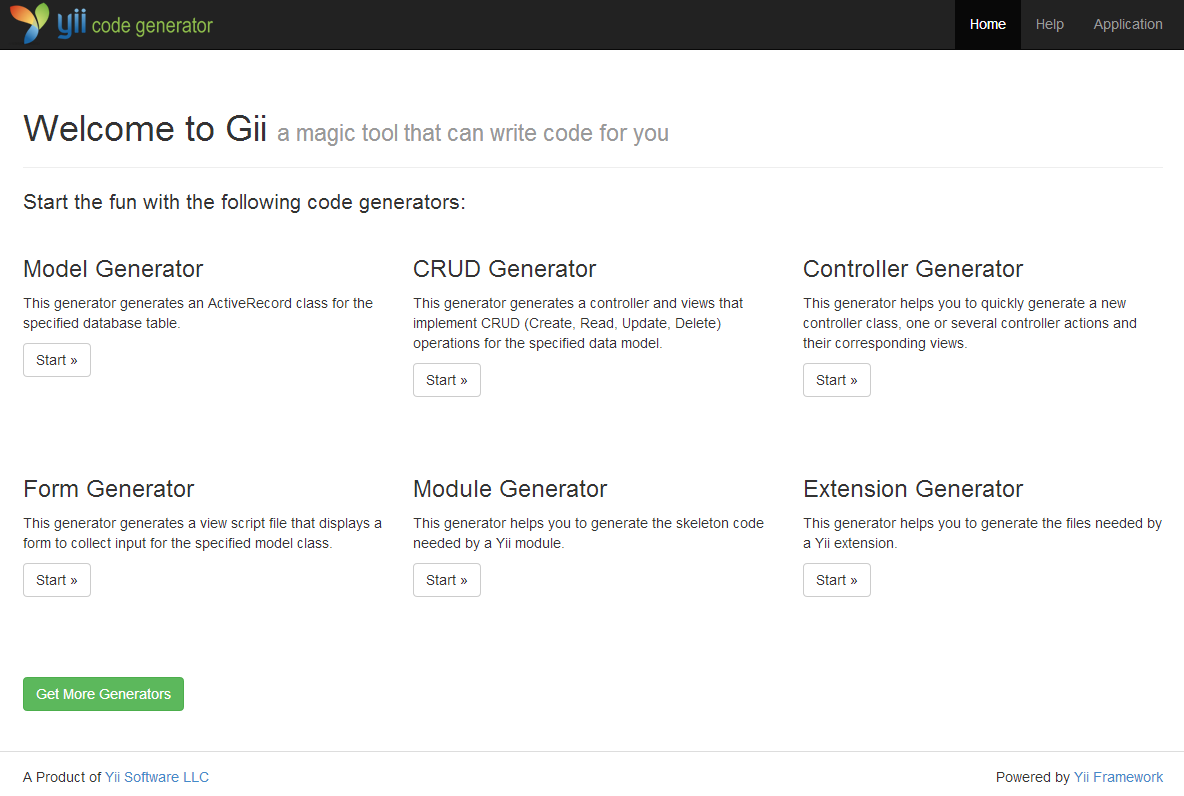
\includegraphics[width=\textwidth]{images/gii-entry.png}

By default there are the following generators available:

\begin{itemize}
\item \textbf{Model Generator} - This generator generates an ActiveRecord class for the specified database table.
\item \textbf{CRUD Generator} - This generator generates a controller and views that implement CRUD (Create, Read, Update, Delete)
operations for the specified data model.
\item \textbf{Controller Generator} - This generator helps you to quickly generate a new controller class, one or several
controller actions and their corresponding views.
\item \textbf{Form Generator} - This generator generates a view script file that displays a form to collect input for the
specified model class.
\item \textbf{Module Generator} - This generator helps you to generate the skeleton code needed by a Yii module.
\item \textbf{Extension Generator} - This generator helps you to generate the files needed by a Yii extension.
\end{itemize}
After choosing a generator by clicking on the ``Start'' button you will see a form that allows you to configure the
parameters of the generator. Fill out the form according to your needs and press the ``Preview'' button to get a
preview of the code that gii is about to generated. Depending on the generator you chose and whether the files
already existed or not, you will get an output similar to what you see in the following picture:

\noindent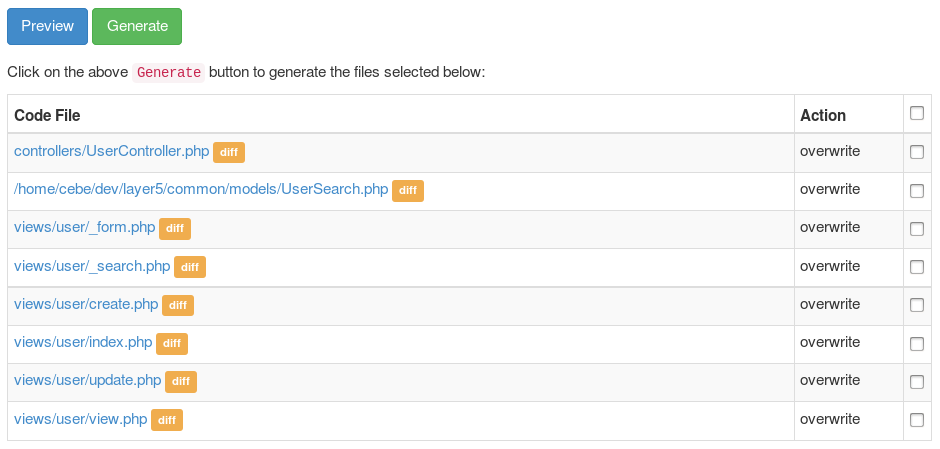
\includegraphics[width=\textwidth]{images/gii-preview.png}

Clicking on the file name you can view a preview of the code that will be generated for that file.
When the file already exists, gii also provides a diff view that shows what is different between the code that exists
and the one that will be generated. In this case you can also choose which files should be overridden and which not.

\begin{quote}Tip: When using the Model Generator to update models after database change, you can copy the code from gii preview
  and merge the changes with your own code. You can use IDE features like PHPStorms
  compare with clipboard\footnote{\url{http://www.jetbrains.com/phpstorm/webhelp/comparing-files.html}} for this,
  which allows you to merge in relevant changes and leave out others that may revert your own code.

\end{quote}
After you have reviewed the code and selected the files to be generated you can click the ``Generate'' button to create
the files. If all went fine you are done. When you see errors that gii is not able to generate the files you have to
adjust directory permissions so that your webserver is able to write to the directories and create the files.

\begin{quote}Note: The code generated by gii is only a template that has to be adjusted to your needs. It is there
  to help you create new things quickly but it is not something that creates ready to use code.
  We often see people using the models generated by gii without change and just extend them to adjust
  some parts of it. This is not how it is meant to be used. Code generated by gii may be incomplete or incorrect
  and has to be changed to fit your needs before you can use it.

\end{quote}
\subsection{Creating your own templates}
Every generator has a form field \lstinline|Code Template| that lets you choose a template to use for code generation.
By default gii only provides one template \lstinline|default| but you can create your own templates that are adjusted to your needs.

If you open a folder \lstinline|@app\vendor\yiisoft\yii2-gii\generators|, you'll see six folders of generators.
\lstinline|`|

\begin{itemize}
\item controller\begin{itemize}
\item crud\begin{itemize}
\item default
\end{itemize}

\end{itemize}

\item extension
\item form
\item model
\item module\lstset{language={}}\begin{lstlisting}
This is name generator. If you open any of these folders, you can see the folder `default`. This folder is name of the template.
\end{lstlisting}

\end{itemize}
Copy folder \lstinline|@app\vendor\yiisoft\yii2-gii\generators\crud\default| to another location, for example \lstinline|@app\myTemplates\crud\|.
Now open this folder and modify any template to fit your desires, for example, add \lstinline|errorSummary| in \lstinline|views\_form.php|:

\lstset{language=php}\begin{lstlisting}
<?php
//...
<div class="<?= Inflector::camel2id(StringHelper::basename($generator->modelClass)) ?>-form">

    <?= "<?php " ?>$form = ActiveForm::begin(); ?>
    <?= "<?=" ?> $form->errorSummary($model) ?> <!-- ADDED HERE -->
    <?php foreach ($safeAttributes as $attribute) {
        echo "    <?= " . $generator->generateActiveField($attribute) . " ?>\n\n";
    } ?>
//...
\end{lstlisting}
Now you need to tell GII about our template.The setting is made in the config file:

\lstset{language=php}\begin{lstlisting}
// config/web.php for basic app
// ...
if (YII_ENV_DEV) {    
    $config['modules']['gii'] = [
        'class' => 'yii\gii\Module',      
        'allowedIPs' => ['127.0.0.1', '::1', '192.168.0.*', '192.168.178.20'],  
        'generators' => [ //here
            'crud' => [ //name generator
                'class' => 'yii\gii\generators\crud\Generator', //class generator
                'templates' => [ //setting for out templates
                    'myCrud' => '@app/myTemplates/crud/default', //name template => path to template
                ]
            ]
        ],
    ];
}
\end{lstlisting}
Open the CRUD generator and you will see that in the field \lstinline|Code Template| of form appeared own template .

\subsection{Creating your own generators}
Open the folder of any generator and you will see two files \lstinline|form.php| and \lstinline|Generator.php|.
One is the form, the second is the class generator. For create your own generator, you need to create or
override these classes in any folder. Again as in the previous paragraph customize configuration:

\lstset{language=php}\begin{lstlisting}
//config/web.php for basic app
//..
if (YII_ENV_DEV) {    
    $config['modules']['gii'] = [
        'class' => 'yii\gii\Module',      
        'allowedIPs' => ['127.0.0.1', '::1', '192.168.0.*', '192.168.178.20'],  
         'generators' => [
            'myCrud' => [
                'class' => 'app\myTemplates\crud\Generator',
                'templates' => [
                    'my' => '@app/myTemplates/crud/default',
                ]
            ]
        ],
    ];
}
\end{lstlisting}
\lstset{language=php}\begin{lstlisting}
// @app/myTemplates/crud/Generator.php
<?php
namespace app\myTemplates\crud;

class Generator extends \yii\gii\Generator
{
    public function getName()
    {
        return 'MY CRUD Generator';
    }

    public function getDescription()
    {
        return 'My crud generator. The same as a native, but he is mine...';
    }
    
    // ...
}
\end{lstlisting}
Open Gii Module and you will see a new generator appears in it.



\label{tool-api-doc.md}\section{Generating Api Documentation}
\begin{quote}Note: This section is under development.

It has no content yet.

\end{quote}


\chapter{测试}
\label{test-overview.md}\section{Testing}
Testing is an important part of software development. Whether we are aware of it or not, we conduct testing continuously.
For example, when we write a class in PHP, we may debug it step by step or simply use echo or die statements to verify
that implementation works according to our initial plan. In case of web application we're entering some test data in forms
to ensure the page interacts with us as expected. The testing process could be automated so that each time when we need
to verify something, we just need to call up the code that do it for us. The code that verifies that result matches what
we've planned is called test and the process of its creation and further execution is known as automated testing, which
is the main topic of testing chapters.

\subsection{Developing with tests}
Test-Driven Development (TDD) and Behavior-Driven Development (BDD) are approaches of developing
software by describing behavior of a piece of code or the whole feature as a set of scenarios or tests before
writing actual code and only then creating the implementation that allows these tests to pass verifying that intended
behavior is achieved.

The process of developing a feature is the following:

\begin{itemize}
\item Create a new test that describes a feature to be implemented.
\item Run new test and make sure it fails. It is expected since there's no implementation yet.
\item Write simple code to make the new test pass.
\item Run all tests and make sure they all pass.
\item Improve code and make sure tests are still OK.
\end{itemize}
After it's done the process is repeated again for another feature or improvement. If existing feature is to be changed,
tests should be changed as well.

\begin{quote}\textbf{Tip}: If you feel that you are losing time doing a lot of small and simple iterations, try covering more by your
test scenario so you do more before executing tests again. If you're debugging too much, try doing the opposite.

\end{quote}
The reason to create tests before doing any implemenation is that it allows you to focus on what do we want to achieve
and fully dive into ``how to do it'' afterwards. Usually it leads to better abstractions and easier test maintenance when
it comes to feature adjustments in for of less coupled components.

So to sum up pros of such approach are the following:

\begin{itemize}
\item Keeps you focused on one thing at a time so both planning and implementation are getting better.
\item Results in test-covering more features in greater detail i.e. if tests are OK most probably nothing's broken.
\end{itemize}
In the long term it usually gives you a good time-saving effect.

\begin{quote}\textbf{Tip}: If you want to know more about the principles for gathering software requirements and modeling the subject
matter it's good to learn Domain Driven Development (DDD)\footnote{\url{https://en.wikipedia.org/wiki/Domain-driven\_design}}.

\end{quote}
\subsection{When and how to test}
While test first approach described above makes sense for long term and relatively complex projects it could be overkill
for simpler ones. There are some indicators of when it's appropriate:

\begin{itemize}
\item Project is already large and complex.
\item Project requirements are starting to get complex. Project grows constantly.
\item Project is meant to be long term.
\item The cost of the failure is too high.
\end{itemize}
There's nothing wrong in creating tests covering behavior of existing implementation.

\begin{itemize}
\item Project is a legacy one to be gradually renewed.
\item You've got a project to work on and it has no tests.
\end{itemize}
In some cases any form of automated testing could be overkill:

\begin{itemize}
\item Project is simple and isn't getting any complex.
\item It's one-time project that's going to be expired.
\end{itemize}
Still if you have time it's good to automate testing in these cases as well.

\subsection{Further reading}
\begin{itemize}
\item Test Driven Development: By Example / Kent Beck. ISBN: 0321146530.
\end{itemize}


\newpage\label{test-endvironment-setup.md}\textbf{Error: not existing file: test-endvironment-setup.md}\newpage
\label{test-unit.md}\section{Unit Tests}
\begin{quote}Note: This section is under development.

\end{quote}
A unit test verifies that a single unit of code is working as expected. In object-oriented programming, the most basic
code unit is a class. A unit test thus mainly needs to verify that each of the class interface methods works properly.
That is, given different input parameters, the test verifies the method returns expected results.
Unit tests are usually developed by people who write the classes being tested.

Unit testing in Yii is built on top of PHPUnit and, optionally, Codeception so it's recommended to go through their docs:

\begin{itemize}
\item PHPUnit docs starting from chapter 2\footnote{\url{http://phpunit.de/manual/current/en/writing-tests-for-phpunit.html}}.
\item Codeception Unit Tests\footnote{\url{http://codeception.com/docs/06-UnitTests}}.
\end{itemize}
\subsection{Running basic and advanced template unit tests}
Please refer to instructions provided in \lstinline|apps/advanced/tests/README.md| and \lstinline|apps/basic/tests/README.md|.



\label{test-functional.md}\section{Functional Tests}
\begin{quote}Note: This section is under development.

\end{quote}
\begin{itemize}
\item \url{http://codeception.com/docs/05-FunctionalTests}
\end{itemize}
\subsection{Running basic and advanced template functional tests}
Please refer to instructions provided in \lstinline|apps/advanced/tests/README.md| and \lstinline|apps/basic/tests/README.md|.



\label{test-acceptance.md}\section{Acceptance Tests}
\begin{quote}Note: This section is under development.

\end{quote}
\begin{itemize}
\item \url{http://codeception.com/docs/04-AcceptanceTests}
\end{itemize}
\subsection{Running basic and advanced template acceptance tests}
Please refer to instructions provided in \lstinline|apps/advanced/tests/README.md| and \lstinline|apps/basic/tests/README.md|.



\label{test-fixtures.md}\section{Fixtures}
\begin{quote}Note: This section is under development.

\end{quote}
Fixtures are important part of testing. Their main purpose is to set up the environment in a fixed/known state
so that your tests are repeatable and run in an expected way. Yii provides a fixture framework that allows
you to define your fixtures precisely and use them easily.

A key concept in the Yii fixture framework is the so-called \textit{fixture objects}. A fixture object represents
a particular aspect of a test environment and is an instance of \texttt{yii{\allowbreak{}\textbackslash}test{\allowbreak{}\textbackslash}Fixture} or its child class. For example,
you may use \lstinline|UserFixture| to make sure the user DB table contains a fixed set of data. You load one or multiple
fixture objects before running a test and unload them when finishing.

A fixture may depend on other fixtures, specified via its \texttt{yii{\allowbreak{}\textbackslash}test{\allowbreak{}\textbackslash}Fixture\allowbreak{}::\allowbreak{}depends} property.
When a fixture is being loaded, the fixtures it depends on will be automatically loaded BEFORE the fixture;
and when the fixture is being unloaded, the dependent fixtures will be unloaded AFTER the fixture.

\subsection{Defining a Fixture}
To define a fixture, create a new class by extending \texttt{yii{\allowbreak{}\textbackslash}test{\allowbreak{}\textbackslash}Fixture} or \texttt{yii{\allowbreak{}\textbackslash}test{\allowbreak{}\textbackslash}ActiveFixture}.
The former is best suited for general purpose fixtures, while the latter has enhanced features specifically
designed to work with database and ActiveRecord.

The following code defines a fixture about the \lstinline|User| ActiveRecord and the corresponding user table.

\lstset{language=php}\begin{lstlisting}
<?php
namespace app\tests\fixtures;

use yii\test\ActiveFixture;

class UserFixture extends ActiveFixture
{
    public $modelClass = 'app\models\User';
}
\end{lstlisting}
\begin{quote}Tip: Each \lstinline|ActiveFixture| is about preparing a DB table for testing purpose. You may specify the table
by setting either the \texttt{yii{\allowbreak{}\textbackslash}test{\allowbreak{}\textbackslash}ActiveFixture\allowbreak{}::\allowbreak{}tableName} property or the \texttt{yii{\allowbreak{}\textbackslash}test{\allowbreak{}\textbackslash}ActiveFixture\allowbreak{}::\allowbreak{}modelClass}
property. If the latter, the table name will be taken from the \lstinline|ActiveRecord| class specified by \lstinline|modelClass|.

\end{quote}
The fixture data for an \lstinline|ActiveFixture| fixture is usually provided in a file located at \lstinline|FixturePath/data/TableName.php|,
where \lstinline|FixturePath| stands for the directory containing the fixture class file, and \lstinline|TableName|
is the name of the table associated with the fixture. In the example above, the file should be
\lstinline|@app/tests/fixtures/data/user.php|. The data file should return an array of data rows
to be inserted into the user table. For example,

\lstset{language=php}\begin{lstlisting}
<?php
return [
    'user1' => [
        'username' => 'lmayert',
        'email' => 'strosin.vernice@jerde.com',
        'auth_key' => 'K3nF70it7tzNsHddEiq0BZ0i-OU8S3xV',
        'password' => '$2y$13$WSyE5hHsG1rWN2jV8LRHzubilrCLI5Ev/iK0r3jRuwQEs2ldRu.a2',
    ],
    'user2' => [
        'username' => 'napoleon69',
        'email' => 'aileen.barton@heaneyschumm.com',
        'auth_key' => 'dZlXsVnIDgIzFgX4EduAqkEPuphhOh9q',
        'password' => '$2y$13$kkgpvJ8lnjKo8RuoR30ay.RjDf15bMcHIF7Vz1zz/6viYG5xJExU6',
    ],
];
\end{lstlisting}
You may give an alias to a row so that later in your test, you may refer to the row via the alias. In the above example,
the two rows are aliased as \lstinline|user1| and \lstinline|user2|, respectively.

Also, you do not need to specify the data for auto-incremental columns. Yii will automatically fill the actual
values into the rows when the fixture is being loaded.

\begin{quote}Tip: You may customize the location of the data file by setting the \texttt{yii{\allowbreak{}\textbackslash}test{\allowbreak{}\textbackslash}ActiveFixture\allowbreak{}::\allowbreak{}dataFile} property.
You may also override \texttt{yii{\allowbreak{}\textbackslash}test{\allowbreak{}\textbackslash}ActiveFixture\allowbreak{}::\allowbreak{}getData()} to provide the data.

\end{quote}
As we described earlier, a fixture may depend on other fixtures. For example, \lstinline|UserProfileFixture| depends on \lstinline|UserFixture|
because the user profile table contains a foreign key pointing to the user table.
The dependency is specified via the \texttt{yii{\allowbreak{}\textbackslash}test{\allowbreak{}\textbackslash}Fixture\allowbreak{}::\allowbreak{}depends} property, like the following,

\lstset{language=php}\begin{lstlisting}
namespace app\tests\fixtures;

use yii\test\ActiveFixture;

class UserProfileFixture extends ActiveFixture
{
    public $modelClass = 'app\models\UserProfile';
    public $depends = ['app\tests\fixtures\UserFixture'];
}
\end{lstlisting}
In the above, we have shown how to define a fixture about a DB table. To define a fixture not related with DB
(e.g. a fixture about certain files and directories), you may extend from the more general base class
\texttt{yii{\allowbreak{}\textbackslash}test{\allowbreak{}\textbackslash}Fixture} and override the \texttt{yii{\allowbreak{}\textbackslash}test{\allowbreak{}\textbackslash}Fixture\allowbreak{}::\allowbreak{}load()} and \texttt{yii{\allowbreak{}\textbackslash}test{\allowbreak{}\textbackslash}Fixture\allowbreak{}::\allowbreak{}unload()} methods.

\subsection{Using Fixtures}
If you are using CodeCeption\footnote{\url{http://codeception.com/}} to test your code, you should consider using
the \lstinline|yii2-codeception| extension which has the built-in support for loading and accessing fixtures.
If you are using other testing frameworks, you may use \texttt{yii{\allowbreak{}\textbackslash}test{\allowbreak{}\textbackslash}FixtureTrait} in your test cases
to achieve the same goal.

In the following we will describe how to write a \lstinline|UserProfile| unit test class using \lstinline|yii2-codeception|.

In your unit test class extending \texttt{yii{\allowbreak{}\textbackslash}codeception{\allowbreak{}\textbackslash}DbTestCase} or \texttt{yii{\allowbreak{}\textbackslash}codeception{\allowbreak{}\textbackslash}TestCase},
declare which fixtures you want to use in the \texttt{yii{\allowbreak{}\textbackslash}test{\allowbreak{}\textbackslash}FixtureTrait\allowbreak{}::\allowbreak{}fixtures()} method. For example,

\lstset{language=php}\begin{lstlisting}
namespace app\tests\unit\models;

use yii\codeception\DbTestCase;
use app\tests\fixtures\UserProfileFixture;

class UserProfileTest extends DbTestCase
{
    public function fixtures()
    {
        return [
            'profiles' => UserProfileFixture::className(),
        ];
    }

    // ...test methods...
}
\end{lstlisting}
The fixtures listed in the \lstinline|fixtures()| method will be automatically loaded before running every test method
in the test case and unloaded after finishing every test method. And as we described before, when a fixture is
being loaded, all its dependent fixtures will be automatically loaded first. In the above example, because
\lstinline|UserProfileFixture| depends on \lstinline|UserFixture|, when running any test method in the test class,
two fixtures will be loaded sequentially: \lstinline|UserFixture| and \lstinline|UserProfileFixture|.

When specifying fixtures in \lstinline|fixtures()|, you may use either a class name or a configuration array to refer to
a fixture. The configuration array will let you customize the fixture properties when the fixture is loaded.

You may also assign an alias to a fixture. In the above example, the \lstinline|UserProfileFixture| is aliased as \lstinline|profiles|.
In the test methods, you may then access a fixture object using its alias. For example, \lstinline|$this->profiles| will
return the \lstinline|UserProfileFixture| object.

Because \lstinline|UserProfileFixture| extends from \lstinline|ActiveFixture|, you may further use the following syntax to access
the data provided by the fixture:

\lstset{language=php}\begin{lstlisting}
// returns the data row aliased as 'user1'
$row = $this->profiles['user1'];
// returns the UserProfile model corresponding to the data row aliased as 'user1'
$profile = $this->profiles('user1');
// traverse every data row in the fixture
foreach ($this->profiles as $row) ...
\end{lstlisting}
\begin{quote}Info: \lstinline|$this->profiles| is still of \lstinline|UserProfileFixture| type. The above access features are implemented
through PHP magic methods.

\end{quote}
\subsection{Defining and Using Global Fixtures}
The fixtures described above are mainly used by individual test cases. In most cases, you also need some global
fixtures that are applied to ALL or many test cases. An example is \texttt{yii{\allowbreak{}\textbackslash}test{\allowbreak{}\textbackslash}InitDbFixture} which does
two things:

\begin{itemize}
\item Perform some common initialization tasks by executing a script located at \lstinline|@app/tests/fixtures/initdb.php|;
\item Disable the database integrity check before loading other DB fixtures, and re-enable it after other DB fixtures are unloaded.
\end{itemize}
Using global fixtures is similar to using non-global ones. The only difference is that you declare these fixtures
in \texttt{yii{\allowbreak{}\textbackslash}codeception{\allowbreak{}\textbackslash}TestCase\allowbreak{}::\allowbreak{}globalFixtures()} instead of \lstinline|fixtures()|. When a test case loads fixtures, it will
first load global fixtures and then non-global ones.

By default, \texttt{yii{\allowbreak{}\textbackslash}codeception{\allowbreak{}\textbackslash}DbTestCase} already declares \lstinline|InitDbFixture| in its \lstinline|globalFixtures()| method.
This means you only need to work with \lstinline|@app/tests/fixtures/initdb.php| if you want to do some initialization work
before each test. You may otherwise simply focus on developing each individual test case and the corresponding fixtures.

\subsection{Organizing Fixture Classes and Data Files}
By default, fixture classes look for the corresponding data files under the \lstinline|data| folder which is a sub-folder
of the folder containing the fixture class files. You can follow this convention when working with simple projects.
For big projects, chances are that you often need to switch different data files for the same fixture class for
different tests. We thus recommend that you organize the data files in a hierarchical way that is similar to
your class namespaces. For example,

\lstset{language={}}\begin{lstlisting}
# under folder tests\unit\fixtures

data\
    components\
        fixture_data_file1.php
        fixture_data_file2.php
        ...
        fixture_data_fileN.php
    models\
        fixture_data_file1.php
        fixture_data_file2.php
        ...
        fixture_data_fileN.php
# and so on
\end{lstlisting}
In this way you will avoid collision of fixture data files between tests and use them as you need.

\begin{quote}Note: In the example above fixture files are named only for example purpose. In real life you should name them
according to which fixture class your fixture classes are extending from. For example, if you are extending
from \texttt{yii{\allowbreak{}\textbackslash}test{\allowbreak{}\textbackslash}ActiveFixture} for DB fixtures, you should use DB table names as the fixture data file names;
If you are extending for \texttt{yii{\allowbreak{}\textbackslash}mongodb{\allowbreak{}\textbackslash}ActiveFixture} for MongoDB fixtures, you should use collection names as the file names.

\end{quote}
The similar hierarchy can be used to organize fixture class files. Instead of using \lstinline|data| as the root directory, you may
want to use \lstinline|fixtures| as the root directory to avoid conflict with the data files.

\subsection{Summary}
In the above, we have described how to define and use fixtures. Below we summarize the typical workflow
of running unit tests related with DB:

\begin{enumerate}
\item Use \lstinline|yii migrate| tool to upgrade your test database to the latest version;
\item Run a test case:\begin{itemize}
\item Load fixtures: clean up the relevant DB tables and populate them with fixture data;
\item Perform the actual test;
\item Unload fixtures.
\end{itemize}

\item Repeat Step 2 until all tests finish.
\end{enumerate}
\textbf{To be cleaned up below}

\section{Managing Fixtures}
// todo: this tutorial may be merged into test-fixture.md

Fixtures are important part of testing. Their main purpose is to populate you with data that needed by testing
different cases. With this data using your tests becoming more efficient and useful.

Yii supports fixtures via the \lstinline|yii fixture| command line tool. This tool supports:

\begin{itemize}
\item Loading fixtures to different storage such as: RDBMS, NoSQL, etc;
\item Unloading fixtures in different ways (usually it is clearing storage);
\item Auto-generating fixtures and populating it with random data.
\end{itemize}
\subsection{Fixtures format}
Fixtures are objects with different methods and configurations, refer to official documentation\footnote{\url{https://github.com/yiisoft/yii2/blob/master/docs/guide/test-fixture.md}} on them.
Lets assume we have fixtures data to load:

\lstset{language={}}\begin{lstlisting}
#users.php file under fixtures data path, by default @tests\unit\fixtures\data

return [
    [
        'name' => 'Chase',
        'login' => 'lmayert',
        'email' => 'strosin.vernice@jerde.com',
        'auth_key' => 'K3nF70it7tzNsHddEiq0BZ0i-OU8S3xV',
        'password' => '$2y$13$WSyE5hHsG1rWN2jV8LRHzubilrCLI5Ev/iK0r3jRuwQEs2ldRu.a2',
    ],
    [
        'name' => 'Celestine',
        'login' => 'napoleon69',
        'email' => 'aileen.barton@heaneyschumm.com',
        'auth_key' => 'dZlXsVnIDgIzFgX4EduAqkEPuphhOh9q',
        'password' => '$2y$13$kkgpvJ8lnjKo8RuoR30ay.RjDf15bMcHIF7Vz1zz/6viYG5xJExU6',
    ],
];
\end{lstlisting}
If we are using fixture that loads data into database then these rows will be applied to \lstinline|users| table. If we are using nosql fixtures, for example \lstinline|mongodb|
fixture, then this data will be applied to \lstinline|users| mongodb collection. In order to learn about implementing various loading strategies and more, refer to official documentation\footnote{\url{https://github.com/yiisoft/yii2/blob/master/docs/guide/test-fixture.md}}.
Above fixture example was auto-generated by \lstinline|yii2-faker| extension, read more about it in these \hyperref[test-fixtures.md::::auto-generating-fixtures]{section}.
Fixture classes name should not be plural.

\subsection{Loading fixtures}
Fixture classes should be suffixed by \lstinline|Fixture| class. By default fixtures will be searched under \lstinline|tests\unit\fixtures| namespace, you can
change this behavior with config or command options. Note that you can also append fixtures data to already existing ones with command
option \lstinline|--append|. You can exclude some fixtures due load or unload by specifying \lstinline|-| before its name like \lstinline|-User|.

To load fixture, run the following command:

\lstset{language={}}\begin{lstlisting}
yii fixture/load <fixture_name>
\end{lstlisting}
The required \lstinline|fixture_name| parameter specifies a fixture name which data will be loaded. You can load several fixtures at once.
Below are correct formats of this command:

\lstset{language={}}\begin{lstlisting}
// load `User` fixture
yii fixture/load User

// same as above, because default action of "fixture" command is "load"
yii fixture User

// load several fixtures
yii fixture User UserProfile

//load fixture, but don't clean storage before load and just append to already existed data
yii fixture User --append

// load all fixtures
yii fixture/load "*"

// same as above
yii fixture "*"

// load all fixtures except ones
yii fixture "*" -DoNotLoadThisOne

// load fixtures, but search them in different namespace. By default namespace is: tests\unit\fixtures.
yii fixture User --namespace='alias\my\custom\namespace'

// load global fixture `some\name\space\CustomFixture` before other fixtures will be loaded.
// By default this option is set to `InitDbFixture` to disable/enable integrity checks. You can specify several
// global fixtures separated by comma.
yii fixture User --globalFixtures='some\name\space\Custom'
\end{lstlisting}
\subsection{Unloading fixtures}
To unload fixture, run the following command:

\lstset{language={}}\begin{lstlisting}
// unload Users fixture, by default it will clear fixture storage (for example "users" table, or "users" collection if this is mongodb fixture).
yii fixture/unload User

// Unload several fixtures
yii fixture/unload User,UserProfile

// unload all fixtures
yii fixture/unload "*"

// unload all fixtures except ones
yii fixture/unload "*" -DoNotUnloadThisOne

\end{lstlisting}
Same command options like: \lstinline|namespace|, \lstinline|globalFixtures| also can be applied to this command.

\subsection{Configure Command Globally}
While command line options allow us to configure the migration command
on-the-fly, sometimes we may want to configure the command once for all. For example you can configure
different migration path as follows:

\lstset{language={}}\begin{lstlisting}
'controllerMap' => [
    'fixture' => [
        'class' => 'yii\console\controllers\FixtureController',
        'namespace' => 'myalias\some\custom\namespace',
        'globalFixtures' => [
            'some\name\space\Foo',
            'other\name\space\Bar'
        ],
    ],
]
\end{lstlisting}
\subsection{Auto-generating fixtures}
Yii also can auto-generate fixtures for you based on some template. You can generate your fixtures with different data on different languages and formats.
These feature is done by Faker\footnote{\url{https://github.com/fzaninotto/Faker}} library and \lstinline|yii2-faker| extension.
See extension guide\footnote{\url{https://github.com/yiisoft/yii2/tree/master/extensions/faker}} for more docs.



\chapter{高级专题}
\label{tutorial-advanced-app.md}\section{Advanced application template}
\begin{quote}Note: This section is under development.

\end{quote}
This template is for large projects developed in teams where the backend is divided from the frontend, application is deployed
to multiple servers etc. This application template also goes a bit further regarding features and provides essential
database, signup and password restore out of the box.

\subsection{Installation}
\subsubsection{Install via Composer}
If you do not have Composer\footnote{\url{http://getcomposer.org/}}, follow the instructions in the
\hyperref[start-installation.md::installing-via-composer]{Installing Yii} section to install it.

With Composer installed, you can then install the application using the following commands:

\lstset{language={}}\begin{lstlisting}
composer global require "fxp/composer-asset-plugin:1.0.0-beta3"
composer create-project --prefer-dist yiisoft/yii2-app-advanced yii-application
\end{lstlisting}
The first command installs the composer asset plugin\footnote{\url{https://github.com/francoispluchino/composer-asset-plugin/}}
which allows managing bower and npm package dependencies through Composer. You only need to run this command
once for all. The second command installs the advanced application in a directory named \lstinline|yii-application|.
You can choose a different directory name if you want.

\subsection{Getting started}
After you install the application, you have to conduct the following steps to initialize
the installed application. You only need to do these once for all.

\begin{enumerate}
\item Execute the \lstinline|init| command and select \lstinline|dev| as environment.

 \lstinline| php /path/to/yii-application/init |

 Otherwise, in production execute \lstinline|init| in non-interactive mode.

 \lstinline| php /path/to/yii-application/init --env=Production overwrite=All |


\item Create a new database and adjust the \lstinline|components.db| configuration in \lstinline|common/config/main-local.php| accordingly.
\item Apply migrations with console command \lstinline|yii migrate|.
\item Set document roots of your web server:
\end{enumerate}
\begin{itemize}
\item for frontend \lstinline|/path/to/yii-application/frontend/web/| and using the URL \lstinline|http://frontend/|
\item for backend \lstinline|/path/to/yii-application/backend/web/| and using the URL \lstinline|http://backend/|
\end{itemize}
\subsection{Directory structure}
The root directory contains the following subdirectories:

\begin{itemize}
\item \lstinline|backend| - backend web application.
\item \lstinline|common| - files common to all applications.
\item \lstinline|console| - console application.
\item \lstinline|environments| - environment configs.
\item \lstinline|frontend| - frontend web application.
\end{itemize}
Root directory contains a set of files.

\begin{itemize}
\item \lstinline|.gitignore| contains a list of directories ignored by git version system. If you need something never get to your source
code repository, add it there.
\item \lstinline|composer.json| - Composer config described in detail below.
\item \lstinline|init| - initialization script described in ``Composer config described in detail below''.
\item \lstinline|init.bat| - same for Windows.
\item \lstinline|LICENSE.md| - license info. Put your project license there. Especially when opensourcing.
\item \lstinline|README.md| - basic info about installing template. Consider replacing it with information about your project and its
installation.
\item \lstinline|requirements.php| - Yii requirements checker.
\item \lstinline|yii| - console application bootstrap.
\item \lstinline|yii.bat| - same for Windows.
\end{itemize}
\subsection{Predefined path aliases}
\begin{itemize}
\item \lstinline|@yii| - framework directory.
\item \lstinline|@app| - base path of currently running application.
\item \lstinline|@common| - common directory.
\item \lstinline|@frontend| - frontend web application directory.
\item \lstinline|@backend| - backend web application directory.
\item \lstinline|@console| - console directory.
\item \lstinline|@runtime| - runtime directory of currently running web application.
\item \lstinline|@vendor| - Composer vendor directory.
\item \lstinline|@bower| - vendor directory that contains the bower packages\footnote{\url{http://bower.io/}}.
\item \lstinline|@npm| - vendor directory that contains npm packages\footnote{\url{https://www.npmjs.org/}}.
\item \lstinline|@web| - base URL of currently running web application.
\item \lstinline|@webroot| - web root directory of currently running web application.
\end{itemize}
The aliases specific to the directory structure of the advanced application
(\lstinline|@common|,  \lstinline|@frontend|, \lstinline|@backend|, and \lstinline|@console|) are defined in \lstinline|common/config/bootstrap.php|.

\subsection{Applications}
There are three applications in advanced template: frontend, backend and console. Frontend is typically what is presented
to end user, the project itself. Backend is admin panel, analytics and such functionality. Console is typically used for
cron jobs and low-level server management. Also it's used during application deployment and handles migrations and assets.

There's also a \lstinline|common| directory that contains files used by more than one application. For example, \lstinline|User| model.

frontend and backend are both web applications and both contain the \lstinline|web| directory. That's the webroot you should point your
web server to.

Each application has its own namespace and alias corresponding to its name. Same applies to common directory.

\subsection{Configuration and environments}
There are multiple problems with a typical approach to configuration:

\begin{itemize}
\item Each team member has its own configuration options. Committing such config will affect other team members.
\item Production database password and API keys should not end up in the repository.
\item There are multiple server environments: development, testing, production. Each should have its own configuration.
\item Defining all configuration options for each case is very repetitive and takes too much time to maintain.
\end{itemize}
In order to solve these issues Yii introduces a simple environments concept. Each environment is represented
by a set of files under the \lstinline|environments| directory. The \lstinline|init| command is used to switch between these. What it really does is
copy everything from the environment directory over to the root directory where all applications are.

Typically environment contains application bootstrap files such as \lstinline|index.php| and config files suffixed with
\lstinline|-local.php|. These are added to \lstinline|.gitignore| and never added to source code repository.

In order to avoid duplication configurations are overriding each other. For example, the frontend reads configuration in the
following order:

\begin{itemize}
\item \lstinline|common/config/main.php|
\item \lstinline|common/config/main-local.php|
\item \lstinline|frontend/config/main.php|
\item \lstinline|frontend/config/main-local.php|
\end{itemize}
Parameters are read in the following order:

\begin{itemize}
\item \lstinline|common/config/params.php|
\item \lstinline|common/config/params-local.php|
\item \lstinline|frontend/config/params.php|
\item \lstinline|frontend/config/params-local.php|
\end{itemize}
The later config file overrides the former.

Here's the full scheme:

\noindent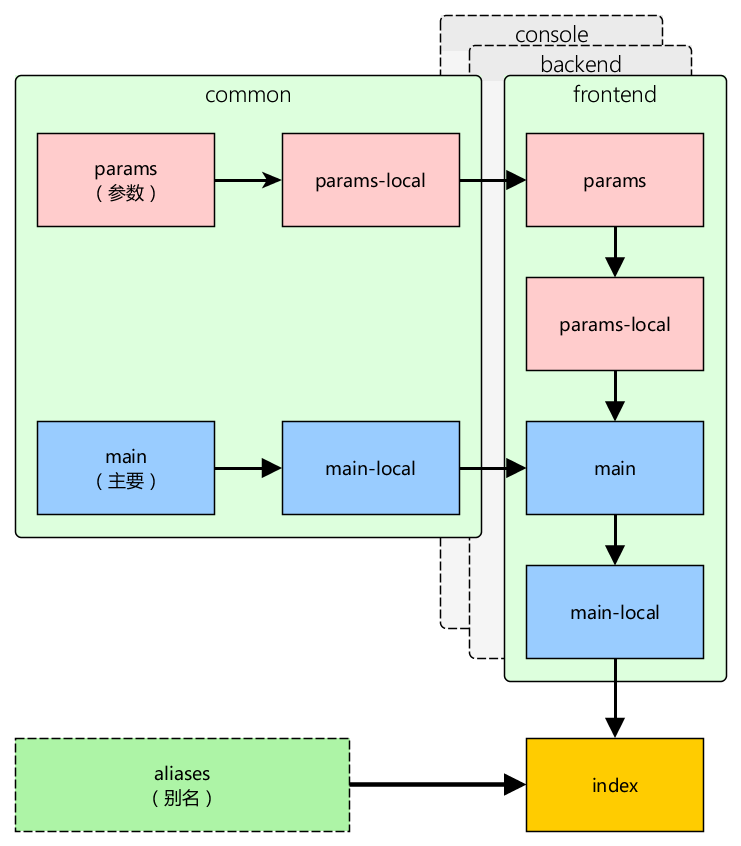
\includegraphics[width=\textwidth]{images/advanced-app-configs.png}

\subsection{Configuring Composer}
After the application template is installed it's a good idea to adjust default \lstinline|composer.json| that can be found in the root
directory:

\lstset{language=json}\begin{lstlisting}
{
    "name": "yiisoft/yii2-app-advanced",
    "description": "Yii 2 Advanced Application Template",
    "keywords": ["yii", "framework", "advanced", "application template"],
    "homepage": "http://www.yiiframework.com/",
    "type": "project",
    "license": "BSD-3-Clause",
    "support": {
        "issues": "https://github.com/yiisoft/yii2/issues?state=open",
        "forum": "http://www.yiiframework.com/forum/",
        "wiki": "http://www.yiiframework.com/wiki/",
        "irc": "irc://irc.freenode.net/yii",
        "source": "https://github.com/yiisoft/yii2"
    },
    "minimum-stability": "dev",
    "require": {
        "php": ">=5.4.0",
        "yiisoft/yii2": "*",
        "yiisoft/yii2-swiftmailer": "*",
        "yiisoft/yii2-bootstrap": "*",
        "yiisoft/yii2-debug": "*",
        "yiisoft/yii2-gii": "*"
    },
    "scripts": {
        "post-create-project-cmd": [
            "yii\\composer\\Installer::setPermission"
        ]
    },
    "extra": {
        "writable": [
            "backend/runtime",
            "backend/web/assets",

            "console/runtime",
            "console/migrations",

            "frontend/runtime",
            "frontend/web/assets"
        ]
    }
}
\end{lstlisting}
First we're updating basic information. Change \lstinline|name|, \lstinline|description|, \lstinline|keywords|, \lstinline|homepage| and \lstinline|support| to match
your project.

Now the interesting part. You can add more packages your application needs to the \lstinline|require| section.
All these packages are coming from packagist.org\footnote{\url{https://packagist.org/}} so feel free to browse the website for useful code.

After your \lstinline|composer.json| is changed you can run \lstinline|composer update --prefer-dist|, wait till packages are downloaded and
installed and then just use them. Autoloading of classes will be handled automatically.

\subsection{Creating links from backend to frontend}
Often it's required to create links from the backend application to the frontend application. Since the frontend application may
contain its own URL manager rules you need to duplicate that for the backend application by naming it differently:

\lstset{language=php}\begin{lstlisting}
return [
    'components' => [
        'urlManager' => [
            // here is your normal backend url manager config
        ],
        'urlManagerFrontend' => [
            // here is your frontend URL manager config
        ],

    ],
];
\end{lstlisting}
After it is done, you can get an URL pointing to frontend like the following:

\lstset{language=php}\begin{lstlisting}
echo Yii::$app->urlManagerFrontend->createUrl(...);
\end{lstlisting}


\label{tutorial-start-from-scratch.md}\section{Creating your own Application structure}
\begin{quote}Note: This section is under development.

\end{quote}
While the basic\footnote{\url{https://github.com/yiisoft/yii2/tree/master/apps/basic}} and advanced\footnote{\url{https://github.com/yiisoft/yii2/tree/master/apps/advanced}}
application templates are great for most of your needs, you may want to create your own application template with which
to start your projects.

Application templates in Yii are simply repositories containing a \lstinline|composer.json| file, and registered as a Composer package.
Any repository can be identified as a Composer package, making it installable via \lstinline|create-project| Composer command.

Since it's a bit too much to start building your entire template from scratch, it is better to use one of the built-in
templates as a base. Let's use the basic template here.

\subsection{Clone the Basic Template}
The first step is to clone the basic Yii template's Git repository:

\lstset{language=bash}\begin{lstlisting}
git clone git@github.com:yiisoft/yii2-app-basic.git
\end{lstlisting}
Then wait for the repository to be downloaded to your computer. Since the changes made to the template won't be pushed back, you can delete the \lstinline|.git| diretory and all
of its contents from the download.

\subsection{Modify the Files}
Next, you'll want to modify the \lstinline|composer.json| to reflect your template. Change the \lstinline|name|, \lstinline|description|, \lstinline|keywords|, \lstinline|homepage|, \lstinline|license|, and \lstinline|support| values
to describe your new template. Also adjust the \lstinline|require|, \lstinline|require-dev|, \lstinline|suggest|, and other options to match your template's requirements.

\begin{quote}Note: In the \lstinline|composer.json| file, use the \lstinline|writable| parameter under \lstinline|extra| to specify
per file permissions to be set after an application is created using the template.

\end{quote}
Next, actually modify the structure and contents of the application as you would like the default to be. Finally, update the README file to be applicable to your template.

\subsection{Make a Package}
With the template defined, create a Git repository from it, and push your files there. If you're going to open source your template, Github\footnote{\url{http://github.com}} is the best place to host it. If you intend to keep your template non-collaborative, any Git repository site will do.

Next, you need to register your package for Composer's sake. For public templates, the package should be registered at Packagist\footnote{\url{https://packagist.org/}}.
For private templates, it is a bit more tricky to register the package. For instructions, see the Composer documentation\footnote{\url{https://getcomposer.org/doc/05-repositories.md\#hosting-your-own}}.

\subsection{Use the Template}
That's all that's required to create a new Yii application template. Now you can create projects using your template:

\lstset{language={}}\begin{lstlisting}
composer global require "fxp/composer-asset-plugin:1.0.0-beta3"
composer create-project --prefer-dist --stability=dev mysoft/yii2-app-coolone new-project
\end{lstlisting}


\label{tutorial-console.md}\section{Console applications}
\begin{quote}Note: This section is under development.

\end{quote}
Yii has full featured support for console applications, whose structure is very similar to a Yii web application. A console application
consists of one or more \texttt{yii{\allowbreak{}\textbackslash}console{\allowbreak{}\textbackslash}Controller} classes, which are often referred to as ``commands'' in the console environment. Each controller can also have one or more actions, just like web controllers.

\subsection{Usage \label{tutorial-console.md::usage}}
You execute a console controller action using the following syntax:

\lstset{language={}}\begin{lstlisting}
yii <route> [--option1=value1 --option2=value2 ... argument1 argument2 ...]
\end{lstlisting}
For example, the \texttt{yii{\allowbreak{}\textbackslash}console{\allowbreak{}\textbackslash}controllers{\allowbreak{}\textbackslash}MigrateController\allowbreak{}::\allowbreak{}actionCreate()}
with \texttt{yii{\allowbreak{}\textbackslash}console{\allowbreak{}\textbackslash}controllers{\allowbreak{}\textbackslash}MigrateController\allowbreak{}::\allowbreak{}\$migrationTable} set can
be called from command line like so:

\lstset{language={}}\begin{lstlisting}
yii migrate/create --migrationTable=my_migration
\end{lstlisting}
In the above \lstinline|yii| is the console application entry script which is described below.

\begin{quote}\textbf{Note}: When using \lstinline|*| in console don't forget to quote it as \lstinline|"*"| in order to avoid executing it as a shell
glob that will be replaced by all file names of the current directory.

\end{quote}
\subsection{Entry script \label{tutorial-console.md::entry-script}}
The console application entry script is equivalent to the \lstinline|index.php| bootstrap file used for the web application.
The console entry script is typically called \lstinline|yii|, and located in your application's root directory.
It contains code like the following:

\lstset{language=php}\begin{lstlisting}
#!/usr/bin/env php
<?php
/**
 * Yii console bootstrap file.
 */

defined('YII_DEBUG') or define('YII_DEBUG', true);

// fcgi doesn't have STDIN and STDOUT defined by default
defined('STDIN') or define('STDIN', fopen('php://stdin', 'r'));
defined('STDOUT') or define('STDOUT', fopen('php://stdout', 'w'));

require(__DIR__ . '/vendor/autoload.php');
require(__DIR__ . '/vendor/yiisoft/yii2/Yii.php');

$config = require(__DIR__ . '/config/console.php');

$application = new yii\console\Application($config);
$exitCode = $application->run();
exit($exitCode);
\end{lstlisting}
This script will be created as part of your application; you're free to edit it to suit your needs. The \lstinline|YII_DEBUG| constant can be set \lstinline|false| if you do
not want to see a stack trace on error, and/or if you want to improve the overall performance. In both basic and advanced application
templates, the console application entry script has debugging enabled by default to provide a more developer-friendly environment.

\subsection{Configuration \label{tutorial-console.md::configuration}}
As can be seen in the code above, the console application uses its own configuration file, named \lstinline|console.php|. In this file
you should configure various \hyperref[structure-application-components.md]{application components} and properties for the console application in particular.

If your web application and the console application share a lot of configuration parameters and values, you may consider moving the common
parts into a separate file, and including this file in both of the application configurations (web and console). You can see an example of this in the ``advanced'' application template.

\begin{quote}Tipp: Sometimes, you may want to run a console command using an application configuration that is different
from the one specified in the entry script. For example, you may want to use the \lstinline|yii migrate| command to
upgrade your test databases, which are configured in each individual test suite. To do change the configuration
dynamically, simply specify a custom application configuration
file via the \lstinline|appconfig| option when executing the command:

\lstset{language={}}\begin{lstlisting}
yii <route> --appconfig=path/to/config.php ...
\end{lstlisting}
\end{quote}
\subsection{Creating your own console commands \label{tutorial-console.md::create-command}}
\subsubsection{Console Controller and Action}
A console command is defined as a controller class extending from \texttt{yii{\allowbreak{}\textbackslash}console{\allowbreak{}\textbackslash}Controller}. In the controller class,
you define one or more actions that correspond to sub-commands of the controller. Within each action, you write code that implements the appropriate tasks for that particular sub-command.

When running a command, you need to specify the route to the  controller action. For example,
the route \lstinline|migrate/create| invokes the sub-command that corresponds to the
\texttt{yii{\allowbreak{}\textbackslash}console{\allowbreak{}\textbackslash}controllers{\allowbreak{}\textbackslash}MigrateController\allowbreak{}::\allowbreak{}actionCreate()} action method.
If a route offered during execution does not contain an action ID, the default action will be executed (as with a web controller).

\subsubsection{Options}
By overriding the \texttt{yii{\allowbreak{}\textbackslash}console{\allowbreak{}\textbackslash}Controller\allowbreak{}::\allowbreak{}options()} method, you can specify options that are available
to a console command (controller/actionID). The method should return a list of the controller class's public properties.
When running a command, you may specify the value of an option using the syntax \lstinline|--OptionName=OptionValue|.
This will assign \lstinline|OptionValue| to the \lstinline|OptionName| property of the controller class.

If the default value of an option is of an array type and you set this option while running the command,
the option value will be converted into an array by splitting the input string on any commas.

\subsubsection{Arguments}
Besides options, a command can also receive arguments. The arguments will be passed as the parameters to the action
method corresponding to the requested sub-command. The first argument corresponds to the first parameter, the second
corresponds to the second, and so on. If not enough arguments are provided when the command is called, the corresponding parameters
will take the declared default values, if defined. If no default value is set, and no value is provided at runtime, the command will exit with an error.

You may use the \lstinline|array| type hint to indicate that an argument should be treated as an array. The array will be generated
by splitting the input string on commas.

The follow examples show how to declare arguments:

\lstset{language=php}\begin{lstlisting}
class ExampleController extends \yii\console\Controller
{
    // The command "yii example/create test" will call "actionCreate('test')"
    public function actionCreate($name) { ... }

    // The command "yii example/index city" will call "actionIndex('city', 'name')"
    // The command "yii example/index city id" will call "actionIndex('city', 'id')"
    public function actionIndex($category, $order = 'name') { ... }

    // The command "yii example/add test" will call "actionAdd(['test'])"
    // The command "yii example/add test1,test2" will call "actionAdd(['test1', 'test2'])"
    public function actionAdd(array $name) { ... }
}
\end{lstlisting}
\subsubsection{Exit Code}
Using exit codes is a best practice for console application development. Conventionally, a command returns \lstinline|0| to indicate that
everything is OK. If the command returns a number greater than zero, that's considered to be indicative of an error. The number returned will be the error
code, potentially usable to find out details about the error.
For example \lstinline|1| could stand generally for an unknown error and all codes above would be reserved for specific cases: input errors, missing files, and so forth.

To have your console command return an exit code, simply return an integer in the controller action
method:

\lstset{language=php}\begin{lstlisting}
public function actionIndex()
{
    if (/* some problem */) {
        echo "A problem occured!\n";
        return 1;
    }
    // do something
    return 0;
}
\end{lstlisting}
There are some predefined constants you can use:

\begin{itemize}
\item \lstinline|Controller::EXIT_CODE_NORMAL| with value of \lstinline|0|;
\item \lstinline|Controller::EXIT_CODE_ERROR| with value of \lstinline|1|.
\end{itemize}
It's a good practice to define meaningful constants for your controller in case you have more error code types.

\subsubsection{Formatting and colors}
Yii console supports formatted output that is automatically degraded to non-formatted one if it's not supported
by terminal running the command.

Outputting formatted strings is simple. Here's how to output some bold text:

\lstset{language=php}\begin{lstlisting}
$this->stdout("Hello?\n", Console::BOLD);
\end{lstlisting}
If you need to build string dynamically combining multiple styles it's better to use \lstinline|ansiFormat|:

\lstset{language=php}\begin{lstlisting}
$name = $this->ansiFormat('Alex', Console::FG_YELLOW);
echo "Hello, my name is $name.";
\end{lstlisting}


\label{tutorial-core-validators.md}\section{核心验证器(Core Validators)}
Yii 提供一系列常用的核心验证器,主要存在于 \lstinline|yii\validators| 命名空间之下。为了避免使用冗长的类名,你可以直接用\textbf{昵称}来指定相应的核心验证器。比如你可以用 \lstinline|required| 昵称代指 \texttt{yii{\allowbreak{}\textbackslash}validators{\allowbreak{}\textbackslash}RequiredValidator} 类:

\lstset{language=php}\begin{lstlisting}
public function rules()
{
    return [
        [['email', 'password'], 'required'],
    ];
}
\end{lstlisting}
\texttt{yii{\allowbreak{}\textbackslash}validators{\allowbreak{}\textbackslash}Validator\allowbreak{}::\allowbreak{}builtInValidators} 属性声明了所有被支持的验证器昵称。

下面,我们将详细介绍每一款验证器的主要用法和属性。

\subsection{\texttt{yii{\allowbreak{}\textbackslash}validators{\allowbreak{}\textbackslash}BooleanValidator} \label{tutorial-core-validators.md::boolean}}
\lstset{language=php}\begin{lstlisting}
[
    // 检查 "selected" 是否为 0 或 1,无视数据类型
    ['selected', 'boolean'],

    // 检查 "deleted" 是否为布尔类型,即 true 或 false
    ['deleted', 'boolean', 'trueValue' => true, 'falseValue' => false, 'strict' => true],
]
\end{lstlisting}
该验证器检查输入值是否为一个布尔值。

\begin{itemize}
\item \lstinline|trueValue|: 代表\textbf{真}的值。默认为 \lstinline|'1'|。
\item \lstinline|falseValue|:代表\textbf{假}的值。默认为 \lstinline|'0'|。
\item \lstinline|strict|:是否要求待测输入必须严格匹配 \lstinline|trueValue| 或 \lstinline|falseValue|。默认为 \lstinline|false|。
\end{itemize}
\begin{quote}注意:因为通过 HTML 表单传递的输入数据都是字符串类型,所以一般情况下你都需要保持
  \texttt{yii{\allowbreak{}\textbackslash}validators{\allowbreak{}\textbackslash}BooleanValidator\allowbreak{}::\allowbreak{}strict} 属性为假。

\end{quote}
\subsection{\texttt{yii{\allowbreak{}\textbackslash}captcha{\allowbreak{}\textbackslash}CaptchaValidator} \label{tutorial-core-validators.md::captcha}}
\lstset{language=php}\begin{lstlisting}
[
    ['verificationCode', 'captcha'],
]
\end{lstlisting}
该验证器通常配合 \texttt{yii{\allowbreak{}\textbackslash}captcha{\allowbreak{}\textbackslash}CaptchaAction} 以及 \texttt{yii{\allowbreak{}\textbackslash}captcha{\allowbreak{}\textbackslash}Captcha}
使用,以确保某一输入与 \texttt{yii{\allowbreak{}\textbackslash}captcha{\allowbreak{}\textbackslash}Captcha} 小部件所显示的验证代码(verification code)相同。

\begin{itemize}
\item \lstinline|caseSensitive|:对验证代码的比对是否要求大小写敏感。默认为 false。
\item \lstinline|captchaAction|:指向用于渲染 CAPTCHA 图片的 \texttt{yii{\allowbreak{}\textbackslash}captcha{\allowbreak{}\textbackslash}CaptchaAction} 的 \hyperref[structure-controllers.md::routes]{路由}。默认为 \lstinline|'site/captcha'|。
\item \lstinline|skipOnEmpty|:当输入为空时,是否跳过验证。默认为 false,也就是输入值为必需项。
\end{itemize}
\subsection{\texttt{yii{\allowbreak{}\textbackslash}validators{\allowbreak{}\textbackslash}CompareValidator} \label{tutorial-core-validators.md::compare}}
\lstset{language=php}\begin{lstlisting}
[
    // 检查 "password" 特性的值是否与 "password_repeat" 的值相同
    ['password', 'compare'],

    // 检查年龄是否大于等于 30
    ['age', 'compare', 'compareValue' => 30, 'operator' => '>='],
]
\end{lstlisting}
该验证器比较两个特定输入值之间的关系是否与 \lstinline|operator| 属性所指定的相同。

\begin{itemize}
\item \lstinline|compareAttribute|:用于与原特性相比较的特性名称。当该验证器被用于验证某目标特性时,该属性会默认为目标属性加后缀 \lstinline|_repeat|。举例来说,若目标特性为 \lstinline|password|,则该属性默认为 \lstinline|password_repeat|。
\item \lstinline|compareValue|:用于与输入值相比较的常量值。当该属性与 \lstinline|compareAttribute| 属性同时被指定时,该属性优先被使用。
\item \lstinline|operator|:比较操作符。默认为 \lstinline|==|,意味着检查输入值是否与 \lstinline|compareAttribute| 或 \lstinline|compareValue| 的值相等。该属性支持如下操作符:\begin{itemize}
\item \lstinline|==|:检查两值是否相等。比对为非严格模式。
\item \lstinline|===|:检查两值是否全等。比对为严格模式。
\item \lstinline|!=|:检查两值是否不等。比对为非严格模式。
\item \lstinline|!==|:检查两值是否不全等。比对为严格模式。
\item \lstinline|>|:检查待测目标值是否大于给定被测值。
\item \lstinline|>=|:检查待测目标值是否大于等于给定被测值。
\item \lstinline|<|:检查待测目标值是否小于给定被测值。
\item \lstinline|<=|:检查待测目标值是否小于等于给定被测值。
\end{itemize}

\end{itemize}
\subsection{\texttt{yii{\allowbreak{}\textbackslash}validators{\allowbreak{}\textbackslash}DateValidator} \label{tutorial-core-validators.md::date}}
\lstset{language=php}\begin{lstlisting}
[
    [['from', 'to'], 'date'],
]
\end{lstlisting}
该验证器检查输入值是否为适当格式的 date,time,或者 datetime。另外,它还可以帮你把输入值转换为一个 UNIX 时间戳并保存到 \texttt{yii{\allowbreak{}\textbackslash}validators{\allowbreak{}\textbackslash}DateValidator\allowbreak{}::\allowbreak{}timestampAttribute} 属性所指定的特性里。

\begin{itemize}
\item \lstinline|format|:待测的 日期/时间 格式。请参考
date\_create\_from\_format() 相关的 PHP 手册\footnote{\url{http://www.php.net/manual/zh/datetime.createfromformat.php}}了解设定格式字符串的更多细节。默认值为 \lstinline|'Y-m-d'|。
\item \lstinline|timestampAttribute|:用于保存用输入时间/日期转换出来的 UNIX 时间戳的特性。
\end{itemize}
\subsection{\texttt{yii{\allowbreak{}\textbackslash}validators{\allowbreak{}\textbackslash}DefaultValueValidator} \label{tutorial-core-validators.md::default}}
\lstset{language=php}\begin{lstlisting}
[
    // 若 "age" 为空,则将其设为 null
    ['age', 'default', 'value' => null],

    // 若 "country" 为空,则将其设为 "USA"
    ['country', 'default', 'value' => 'USA'],

    // 若 "from" 和 "to" 为空,则分别给他们分配自今天起,3 天后和 6 天后的日期。
    [['from', 'to'], 'default', 'value' => function ($model, $attribute) {
        return date('Y-m-d', strtotime($attribute === 'to' ? '+3 days' :'+6 days'));
    }],
]
\end{lstlisting}
该验证器并不进行数据验证。而是,给为空的待测特性分配默认值。

\begin{itemize}
\item \lstinline|value|:默认值,或一个返回默认值的 PHP Callable 对象(即回调函数)。它们会分配给检测为空的待测特性。PHP 回调方法的样式如下:
\end{itemize}
\lstset{language=php}\begin{lstlisting}
function foo($model, $attribute) {
    // ... 计算 $value ...
    return $value;
}
\end{lstlisting}
\begin{quote}补充:如何判断待测值是否为空,被写在另外一个话题的\hyperref[input-validation.md::handling-empty-inputs]{处理空输入}章节。

\end{quote}
\subsection{\texttt{yii{\allowbreak{}\textbackslash}validators{\allowbreak{}\textbackslash}NumberValidator} \label{tutorial-core-validators.md::double}}
\lstset{language=php}\begin{lstlisting}
[
    // 检查 "salary" 是否为浮点数
    ['salary', 'double'],
]
\end{lstlisting}
该验证器检查输入值是否为双精度浮点数。他等效于 \hyperref[tutorial-core-validators.md::::number]{number} 验证器。

\begin{itemize}
\item \lstinline|max|:上限值(含界点)。若不设置,则验证器不检查上限。
\item \lstinline|min|:下限值(含界点)。若不设置,则验证器不检查下限。
\end{itemize}
\subsection{\texttt{yii{\allowbreak{}\textbackslash}validators{\allowbreak{}\textbackslash}EmailValidator} \label{tutorial-core-validators.md::email}}
\lstset{language=php}\begin{lstlisting}
[
    // 检查 "email" 是否为有效的邮箱地址
    ['email', 'email'],
]
\end{lstlisting}
该验证器检查输入值是否为有效的邮箱地址。

\begin{itemize}
\item \lstinline|allowName|:检查是否允许带名称的电子邮件地址 (e.g. \lstinline|张三 <John.san@example.com>|)。 默认为 false。
\item \lstinline|checkDNS|:检查邮箱域名是否存在,且有没有对应的 A 或 MX 记录。不过要知道,有的时候该项检查可能会因为临时性 DNS 故障而失败,哪怕它其实是有效的。默认为 false。
\item \lstinline|enableIDN|:验证过程是否应该考虑 IDN(internationalized domain names,国际化域名,也称多语种域名,比如中文域名)。默认为 false。要注意但是为使用 IDN 验证功能,请先确保安装并开启 \lstinline|intl| PHP 扩展,不然会导致抛出异常。
\end{itemize}
\subsection{\texttt{yii{\allowbreak{}\textbackslash}validators{\allowbreak{}\textbackslash}ExistValidator} \label{tutorial-core-validators.md::exist}}
\lstset{language=php}\begin{lstlisting}
[
    // a1 需要在 "a1" 特性所代表的字段内存在
    ['a1', 'exist'],

    // a1 必需存在,但检验的是 a1 的值在字段 a2 中的存在性
    ['a1', 'exist', 'targetAttribute' => 'a2'],

    // a1 和 a2 的值都需要存在,且它们都能收到错误提示
    [['a1', 'a2'], 'exist', 'targetAttribute' => ['a1', 'a2']],

    // a1 和 a2 的值都需要存在,只有 a1 能接收到错误信息
    ['a1', 'exist', 'targetAttribute' => ['a1', 'a2']],

    // 通过同时在 a2 和 a3 字段中检查 a2 和 a1 的值来确定 a1 的存在性
    ['a1', 'exist', 'targetAttribute' => ['a2', 'a1' => 'a3']],

    // a1 必需存在,若 a1 为数组,则其每个子元素都必须存在。
    ['a1', 'exist', 'allowArray' => true],
]
\end{lstlisting}
该验证器检查输入值是否在某表字段中存在。它只对\hyperref[db-active-record.md]{活动记录}类型的模型类特性起作用,能支持对一个或多过字段的验证。

\begin{itemize}
\item \lstinline|targetClass|:用于查找输入值的目标 \hyperref[db-active-record.md]{AR} 类。若不设置,则会使用正在进行验证的当前模型类。
\item \lstinline|targetAttribute|:用于检查输入值存在性的 \lstinline|targetClass| 的模型特性。\begin{itemize}
\item 若不设置,它会直接使用待测特性名(整个参数数组的首元素)。
\item 除了指定为字符串以外,你也可以用数组的形式,同时指定多个用于验证的表字段,数组的键和值都是代表字段的特性名,值表示 \lstinline|targetClass| 的待测数据源字段,而键表示当前模型的待测特性名。
\item 若键和值相同,你可以只指定值。(如:\lstinline|['a2']| 就代表 \lstinline|['a2'=>'a2']|)
\end{itemize}

\item \lstinline|filter|:用于检查输入值存在性必然会进行数据库查询,而该属性为用于进一步筛选该查询的过滤条件。可以为代表额外查询条件的字符串或数组(关于查询条件的格式,请参考 \texttt{yii{\allowbreak{}\textbackslash}db{\allowbreak{}\textbackslash}Query\allowbreak{}::\allowbreak{}where()});或者样式为 \lstinline|function ($query)| 的匿名函数,\lstinline|$query| 参数为你希望在该函数内进行修改的 \texttt{yii{\allowbreak{}\textbackslash}db{\allowbreak{}\textbackslash}Query} 对象。
\item \lstinline|allowArray|:是否允许输入值为数组。默认为 false。若该属性为 true 且输入值为数组,则数组的每个元素都必须在目标字段中存在。值得注意的是,若用吧 \lstinline|targetAttribute| 设为多元素数组来验证被测值在多字段中的存在性时,该属性不能设置为 true。
\end{itemize}
\begin{quote}译者注:\hyperref[tutorial-core-validators.md::::exist]{exist} 和 \hyperref[tutorial-core-validators.md::::unique]{unique} 验证器的机理和参数都相似,有点像一体两面的阴和阳。

\begin{itemize}
\item 他们的区别是 exist 要求 \lstinline|targetAttribute| 键所代表的的属性在其值所代表字段中找得到;而 unique 正相反,要求键所代表的的属性不能在其值所代表字段中被找到。
\item 从另一个角度来理解:他们都会在验证的过程中执行数据库查询,查询的条件即为where \$v=\$k (假设 \lstinline|targetAttribute| 的其中一对键值对为 \lstinline|$k => $v|)。unique 要求查询的结果数 \lstinline|$count==0|,而 exist 则要求查询的结果数 \lstinline|$count>0|
\item 最后别忘了,unique 验证器不存在 \lstinline|allowArray| 属性哦。
\end{itemize}
\end{quote}
\subsection{\texttt{yii{\allowbreak{}\textbackslash}validators{\allowbreak{}\textbackslash}FileValidator} \label{tutorial-core-validators.md::file}}
\lstset{language=php}\begin{lstlisting}
[
    // 检查 "primaryImage" 是否为 PNG, JPG 或 GIF 格式的上传图片。
    // 文件大小必须小于  1MB
    ['primaryImage', 'file', 'extensions' => ['png', 'jpg', 'gif'], 'maxSize' => 1024*1024*1024],
]
\end{lstlisting}
该验证器检查输入值是否为一个有效的上传文件。

\begin{itemize}
\item \lstinline|extensions|:可接受上传的文件扩展名列表。它可以是数组,也可以是用空格或逗号分隔各个扩展名的字符串 (e.g. ``gif, jpg'')。
扩展名大小写不敏感。默认为 null,意味着所有扩展名都被接受。
\item \lstinline|mimeTypes|:可接受上传的 MIME 类型列表。它可以是数组,也可以是用空格或逗号分隔各个 MIME 的字符串 (e.g. ``image/jpeg, image/png'')。
Mime 类型名是大小写不敏感的。默认为 null,意味着所有 MIME 类型都被接受。
\item \lstinline|minSize|:上传文件所需最少多少 Byte 的大小。默认为 null,代表没有下限。
\item \lstinline|maxSize|:上传文件所需最多多少 Byte 的大小。默认为 null,代表没有上限。
\item \lstinline|maxFiles|:给定特性最多能承载多少个文件。默认为 1,代表只允许单文件上传。若值大于一,那么输入值必须为包含最多 \lstinline|maxFiles| 个上传文件元素的数组。
\item \lstinline|checkExtensionByMimeType|:是否通过文件的 MIME 类型来判断其文件扩展。若由 MIME 判定的文件扩展与给定文件的扩展不一样,则文件会被认为无效。默认为 true,代表执行上述检测。
\end{itemize}
\lstinline|FileValidator| 通常与 \texttt{yii{\allowbreak{}\textbackslash}web{\allowbreak{}\textbackslash}UploadedFile} 共同使用。请参考 \hyperref[input-file-upload.md]{文件上传}章节来了解有关文件上传与上传文件的检验的全部内容。

\subsection{\texttt{yii{\allowbreak{}\textbackslash}validators{\allowbreak{}\textbackslash}FilterValidator} \label{tutorial-core-validators.md::filter}}
\lstset{language=php}\begin{lstlisting}
[
    // trim 掉 "username" 和 "email" 输入
    [['username', 'email'], 'filter', 'filter' => 'trim', 'skipOnArray' => true],

    // 标准化 "phone" 输入
    ['phone', 'filter', 'filter' => function ($value) {
        // 在此处标准化输入的电话号码
        return $value;
    }],
]
\end{lstlisting}
该验证器并不进行数据验证。而是,给输入值应用一个滤镜,并在检验过程之后把它赋值回特性变量。

\begin{itemize}
\item \lstinline|filter|:用于定义滤镜的 PHP 回调函数。可以为全局函数名,匿名函数,或其他。该函数的样式必须是 \lstinline|function ($value) { return $newValue; }|。该属性不能省略,必须设置。
\item \lstinline|skipOnArray|:是否在输入值为数组时跳过滤镜。默认为 false。请注意如果滤镜不能处理数组输入,你就应该把该属性设为 true。否则可能会导致 PHP Error 的发生。
\end{itemize}
\begin{quote}技巧:如果你只是想要用 trim 处理下输入值,你可以直接用 \hyperref[tutorial-core-validators.md::::trim]{trim} 验证器的。

\end{quote}
\subsection{\texttt{yii{\allowbreak{}\textbackslash}validators{\allowbreak{}\textbackslash}ImageValidator} \label{tutorial-core-validators.md::image}}
\lstset{language=php}\begin{lstlisting}
[
    // 检查 "primaryImage" 是否为适当尺寸的有效图片
    ['primaryImage', 'image', 'extensions' => 'png, jpg',
        'minWidth' => 100, 'maxWidth' => 1000,
        'minHeight' => 100, 'maxHeight' => 1000,
    ],
]
\end{lstlisting}
该验证器检查输入值是否为代表有效的图片文件。它继承自 \hyperref[tutorial-core-validators.md::::file]{file} 验证器,并因此继承有其全部属性。除此之外,它还支持以下为图片检验而设的额外属性:

\begin{itemize}
\item \lstinline|minWidth|:图片的最小宽度。默认为 null,代表无下限。
\item \lstinline|maxWidth|:图片的最大宽度。默认为 null,代表无上限。
\item \lstinline|minHeight|:图片的最小高度。 默认为 null,代表无下限。
\item \lstinline|maxHeight|:图片的最大高度。默认为 null,代表无上限。
\end{itemize}
\subsection{\texttt{yii{\allowbreak{}\textbackslash}validators{\allowbreak{}\textbackslash}RangeValidator} \label{tutorial-core-validators.md::in}}
\lstset{language=php}\begin{lstlisting}
[
    // 检查 "level" 是否为 1、2 或 3 中的一个
    ['level', 'in', 'range' => [1, 2, 3]],
]
\end{lstlisting}
该验证器检查输入值是否存在于给定列表的范围之中。

\begin{itemize}
\item \lstinline|range|:用于检查输入值的给定值列表。
\item \lstinline|strict|:输入值与给定值直接的比较是否为严格模式(也就是类型与值都要相同,即全等)。默认为 false。
\item \lstinline|not|:是否对验证的结果取反。默认为 false。当该属性被设置为 true,验证器检查输入值是否\textbf{不在}给定列表内。
\item \lstinline|allowArray|:是否接受输入值为数组。当该值为 true 且输入值为数组时,数组内的每一个元素都必须在给定列表内存在,否则返回验证失败。
\end{itemize}
\subsection{\texttt{yii{\allowbreak{}\textbackslash}validators{\allowbreak{}\textbackslash}NumberValidator} \label{tutorial-core-validators.md::integer}}
\lstset{language=php}\begin{lstlisting}
[
    // 检查 "age" 是否为整数
    ['age', 'integer'],
]
\end{lstlisting}
该验证器检查输入值是否为整形。

\begin{itemize}
\item \lstinline|max|:上限值(含界点)。若不设置,则验证器不检查上限。
\item \lstinline|min|:下限值(含界点)。若不设置,则验证器不检查下限。
\end{itemize}
\subsection{\texttt{yii{\allowbreak{}\textbackslash}validators{\allowbreak{}\textbackslash}RegularExpressionValidator} \label{tutorial-core-validators.md::match}}
\lstset{language=php}\begin{lstlisting}
[
    // 检查 "username" 是否由字母开头,且只包含单词字符
    ['username', 'match', 'pattern' => '/^[a-z]\w*$/i']
]
\end{lstlisting}
该验证器检查输入值是否匹配指定正则表达式。

\begin{itemize}
\item \lstinline|pattern|:用于检测输入值的正则表达式。该属性是必须的,若不设置则会抛出异常。
\item \lstinline|not|:是否对验证的结果取反。默认为 false,代表输入值匹配正则表达式时验证成功。如果设为 true,则输入值不匹配正则时返回匹配成功。
\end{itemize}
\subsection{\texttt{yii{\allowbreak{}\textbackslash}validators{\allowbreak{}\textbackslash}NumberValidator} \label{tutorial-core-validators.md::number}}
\lstset{language=php}\begin{lstlisting}
[
    // 检查 "salary" 是否为数字
    ['salary', 'number'],
]
\end{lstlisting}
该验证器检查输入值是否为数字。他等效于 \hyperref[tutorial-core-validators.md::::double]{double} 验证器。

\begin{itemize}
\item \lstinline|max|:上限值(含界点)。若不设置,则验证器不检查上限。
\item \lstinline|min|:下限值(含界点)。若不设置,则验证器不检查下限。
\end{itemize}
\subsection{\texttt{yii{\allowbreak{}\textbackslash}validators{\allowbreak{}\textbackslash}RequiredValidator} \label{tutorial-core-validators.md::required}}
\lstset{language=php}\begin{lstlisting}
[
    // 检查 "username" 与 "password" 是否为空
    [['username', 'password'], 'required'],
]
\end{lstlisting}
该验证器检查输入值是否为空,还是已经提供了。

\begin{itemize}
\item \lstinline|requiredValue|:所期望的输入值。若没设置,意味着输入不能为空。
\item \lstinline|strict|:检查输入值时是否检查类型。默认为 false。当没有设置 \lstinline|requiredValue| 属性时,若该属性为 true,验证器会检查输入值是否严格为 null;若该属性设为 false,该验证器会用一个更加宽松的规则检验输入值是否为空。
\end{itemize}
当设置了 \lstinline|requiredValue| 属性时,若该属性为 true,输入值与 \lstinline|requiredValue| 的比对会同时检查数据类型。

\begin{quote}补充:如何判断待测值是否为空,被写在另外一个话题的\hyperref[input-validation.md::handling-empty-inputs]{处理空输入}章节。

\end{quote}
\subsection{\texttt{yii{\allowbreak{}\textbackslash}validators{\allowbreak{}\textbackslash}SafeValidator} \label{tutorial-core-validators.md::safe}}
\lstset{language=php}\begin{lstlisting}
[
    // 标记 "description" 为安全特性
    ['description', 'safe'],
]
\end{lstlisting}
该验证器并不进行数据验证。而是把一个特性标记为\hyperref[structure-models.md::safe-attributes]{安全特性}。

\subsection{\texttt{yii{\allowbreak{}\textbackslash}validators{\allowbreak{}\textbackslash}StringValidator} \label{tutorial-core-validators.md::string}}
\lstset{language=php}\begin{lstlisting}
[
    // 检查 "username" 是否为长度 4 到 24 之间的字符串
    ['username', 'string', 'length' => [4, 24]],
]
\end{lstlisting}
该验证器检查输入值是否为特定长度的字符串。并检查特性的值是否为某个特定长度。

\begin{itemize}
\item \lstinline|length|:指定待测输入字符串的长度限制。该属性可以被指定为以下格式之一:\begin{itemize}
\item 证书:the exact length that the string should be of;
\item 单元素数组:代表输入字符串的最小长度 (e.g. \lstinline|[8]|)。这会重写 \lstinline|min| 属性。
\item 包含两个元素的数组:代表输入字符串的最小和最大长度(e.g. \lstinline|[8, 128]|)。
   这会同时重写 \lstinline|min| 和 \lstinline|max| 属性。
\end{itemize}

\item \lstinline|min|:输入字符串的最小长度。若不设置,则代表不设下限。
\item \lstinline|max|:输入字符串的最大长度。若不设置,则代表不设上限。
\item \lstinline|encoding|:待测字符串的编码方式。若不设置,则使用应用自身的 \texttt{yii{\allowbreak{}\textbackslash}base{\allowbreak{}\textbackslash}Application\allowbreak{}::\allowbreak{}charset} 属性值,该值默认为 \lstinline|UTF-8|。
\end{itemize}
\subsection{\texttt{yii{\allowbreak{}\textbackslash}validators{\allowbreak{}\textbackslash}FilterValidator} \label{tutorial-core-validators.md::trim}}
\lstset{language=php}\begin{lstlisting}
[
    // trim 掉 "username" 和 "email" 两侧的多余空格
    [['username', 'email'], 'trim'],
]
\end{lstlisting}
该验证器并不进行数据验证。而是,trim 掉输入值两侧的多余空格。注意若该输入值为数组,那它会忽略掉该验证器。

\subsection{\texttt{yii{\allowbreak{}\textbackslash}validators{\allowbreak{}\textbackslash}UniqueValidator} \label{tutorial-core-validators.md::unique}}
\lstset{language=php}\begin{lstlisting}
[
    // a1 需要在 "a1" 特性所代表的字段内唯一
    ['a1', 'unique'],

    // a1 需要唯一,但检验的是 a1 的值在字段 a2 中的唯一性
    ['a1', 'unique', 'targetAttribute' => 'a2'],

    // a1 和 a2 的组合需要唯一,且它们都能收到错误提示
    [['a1', 'a2'], 'unique', 'targetAttribute' => ['a1', 'a2']],

    // a1 和 a2 的组合需要唯一,只有 a1 能接收错误提示
    ['a1', 'unique', 'targetAttribute' => ['a1', 'a2']],

    // 通过同时在 a2 和 a3 字段中检查 a2 和 a3 的值来确定 a1 的唯一性
    ['a1', 'unique', 'targetAttribute' => ['a2', 'a1' => 'a3']],
]
\end{lstlisting}
该验证器检查输入值是否在某表字段中唯一。它只对\hyperref[db-active-record.md]{活动记录}类型的模型类特性起作用,能支持对一个或多过字段的验证。

\begin{itemize}
\item \lstinline|targetClass|:用于查找输入值的目标 \hyperref[db-active-record.md]{AR} 类。若不设置,则会使用正在进行验证的当前模型类。
\item \lstinline|targetAttribute|:用于检查输入值唯一性的 \lstinline|targetClass| 的模型特性。\begin{itemize}
\item 若不设置,它会直接使用待测特性名(整个参数数组的首元素)。
\item 除了指定为字符串以外,你也可以用数组的形式,同时指定多个用于验证的表字段,数组的键和值都是代表字段的特性名,值表示 \lstinline|targetClass| 的待测数据源字段,而键表示当前模型的待测特性名。
\item 若键和值相同,你可以只指定值。(如:\lstinline|['a2']| 就代表 \lstinline|['a2'=>'a2']|)
\end{itemize}

\item \lstinline|filter|:用于检查输入值唯一性必然会进行数据库查询,而该属性为用于进一步筛选该查询的过滤条件。可以为代表额外查询条件的字符串或数组(关于查询条件的格式,请参考 \texttt{yii{\allowbreak{}\textbackslash}db{\allowbreak{}\textbackslash}Query\allowbreak{}::\allowbreak{}where()});或者样式为 \lstinline|function ($query)| 的匿名函数,\lstinline|$query| 参数为你希望在该函数内进行修改的 \texttt{yii{\allowbreak{}\textbackslash}db{\allowbreak{}\textbackslash}Query} 对象。
\end{itemize}
\begin{quote}译者注:\hyperref[tutorial-core-validators.md::::exist]{exist} 和 \hyperref[tutorial-core-validators.md::::unique]{unique} 验证器的机理和参数都相似,有点像一体两面的阴和阳。

\begin{itemize}
\item 他们的区别是 exist 要求 \lstinline|targetAttribute| 键所代表的的属性在其值所代表字段中找得到;而 unique 正相反,要求键所代表的的属性不能在其值所代表字段中被找到。
\item 从另一个角度来理解:他们都会在验证的过程中执行数据库查询,查询的条件即为where \$v=\$k (假设 \lstinline|targetAttribute| 的其中一对键值对为 \lstinline|$k => $v|)。unique 要求查询的结果数 \lstinline|$count==0|,而 exist 则要求查询的结果数 \lstinline|$count>0|
\item 最后别忘了,unique 验证器不存在 \lstinline|allowArray| 属性哦。
\end{itemize}
\end{quote}
\subsection{\texttt{yii{\allowbreak{}\textbackslash}validators{\allowbreak{}\textbackslash}UrlValidator} \label{tutorial-core-validators.md::url}}
\lstset{language=php}\begin{lstlisting}
[
    // 检查 "website" 是否为有效的 URL。若没有 URI 方案,则给 "website" 特性加 "http://" 前缀
    ['website', 'url', 'defaultScheme' => 'http'],
]
\end{lstlisting}
该验证器检查输入值是否为有效 URL。

\begin{itemize}
\item \lstinline|validSchemes|:用于指定那些 URI 方案会被视为有效的数组。默认为 \lstinline|['http', 'https']|,代表 \lstinline|http| 和 \lstinline|https| URLs 会被认为有效。
\item \lstinline|defaultScheme|:若输入值没有对应的方案前缀,会使用的默认 URI 方案前缀。默认为 null,代表不修改输入值本身。
\item \lstinline|enableIDN|:验证过程是否应该考虑 IDN(internationalized domain names,国际化域名,也称多语种域名,比如中文域名)。默认为 false。要注意但是为使用 IDN 验证功能,请先确保安装并开启 \lstinline|intl| PHP 扩展,不然会导致抛出异常。
\end{itemize}


\label{tutorial-i18n.md}\section{Internationalization}
\begin{quote}Note: This section is under development.

\end{quote}
Internationalization (I18N) refers to the process of designing a software application so that it can be adapted to
various languages and regions without engineering changes. For Web applications, this is of particular importance
because the potential users may be worldwide.

Yii offers several tools that help with internationalisation of a website such as message translation and
number- and date-formatting.

\subsection{Locale and Language}
There are two languages defined in the Yii application: \texttt{yii{\allowbreak{}\textbackslash}base{\allowbreak{}\textbackslash}Application\allowbreak{}::\allowbreak{}\$sourceLanguage} and
\texttt{yii{\allowbreak{}\textbackslash}base{\allowbreak{}\textbackslash}Application\allowbreak{}::\allowbreak{}\$language}.

Source language is the language original application messages are written in directly in the code such as:

\lstset{language=php}\begin{lstlisting}
echo \Yii::t('app', 'I am a message!');
\end{lstlisting}
The target language is the language that should be used to display the current page i.e. the language that original messages need
to be translated to. It is defined in the application configuration like the following:

\lstset{language=php}\begin{lstlisting}
return [
    'id' => 'applicationID',
    'basePath' => dirname(__DIR__),
    // ...
    'language' => 'ru-RU', // <- here!
    // ...
]
\end{lstlisting}
\begin{quote}\textbf{Tip}: The default value for the \texttt{yii{\allowbreak{}\textbackslash}base{\allowbreak{}\textbackslash}Application\allowbreak{}::\allowbreak{}\$sourceLanguage} is English and it is
recommended to keep this value. The reason is that it's easier to find people translating from
English to any language than from non-English to non-English.

\end{quote}
You may set the application language at runtime to set it to a language the user has chosen.
This has to be done at a point before any output is generated so that it affects all the output correctly.
Therefor just change the application property to the desired value:

\lstset{language=php}\begin{lstlisting}
\Yii::$app->language = 'zh-CN';
\end{lstlisting}
The format for the language/locale is \lstinline|ll-CC| where \lstinline|ll| is a two- or three-letter lowercase code for a language according to
ISO-639\footnote{\url{http://www.loc.gov/standards/iso639-2/}} and \lstinline|CC| is the country code according to
ISO-3166\footnote{\url{http://www.iso.org/iso/en/prods-services/iso3166ma/02iso-3166-code-lists/list-en1.html}}.

\begin{quote}\textbf{Note}: For more information on the concept and syntax of locales, check the
documentation of the ICU project\footnote{\url{http://userguide.icu-project.org/locale\#TOC-The-Locale-Concept}}.

\end{quote}
\subsection{Message translation}
Message translation is used to translate messages that are ouput by an applicaiton to different languages
so that users from different countries can use the application in their native language.

The message translation feature in Yii works simply as finding a
translation of the message from a source language into a target language.
To use the message translation feature you wrap your original message strings with a call to the \texttt{Yii\allowbreak{}::\allowbreak{}t()} method.
The first parameter of this method takes a category which helps to distingish the source of messages in differnet parts
of the application and the second parameter is the message itself.

\lstset{language=php}\begin{lstlisting}
echo \Yii::t('app', 'This is a string to translate!');
\end{lstlisting}
Yii tries to load an appropriate translation according to the current \texttt{yii{\allowbreak{}\textbackslash}base{\allowbreak{}\textbackslash}Application\allowbreak{}::\allowbreak{}\$language}
from one of the message sources defined in the \lstinline|i18n| \hyperref[structure-application-components.md]{application component}.
A message source is a set of files or a database that provides translation messages.
The following configuration example defines a messages source that takes the messages from PHP files:

\lstset{language=php}\begin{lstlisting}
'components' => [
    // ...
    'i18n' => [
        'translations' => [
            'app*' => [
                'class' => 'yii\i18n\PhpMessageSource',
                //'basePath' => '@app/messages',
                //'sourceLanguage' => 'en-US',
                'fileMap' => [
                    'app' => 'app.php',
                    'app/error' => 'error.php',
                ],
            ],
        ],
    ],
],
\end{lstlisting}
In the above \lstinline|app*| is a pattern that specifies which categories are handled by the message source. In this case we're
handling everything that begins with \lstinline|app|. Message files are located in \lstinline|@app/messages|, the \lstinline|messages| directory
in your application directory. The \texttt{yii{\allowbreak{}\textbackslash}i18n{\allowbreak{}\textbackslash}PhpMessageSource\allowbreak{}::\allowbreak{}fileMap} array
defines which file is to be used for which category.
Instead of configuring \lstinline|fileMap| you can rely on convention which is to use the category name as the file name
(e.g. category \lstinline|app/error| will result in the file name \lstinline|app/error.php| under the \texttt{yii{\allowbreak{}\textbackslash}i18n{\allowbreak{}\textbackslash}PhpMessageSource\allowbreak{}::\allowbreak{}basePath}.

When translating the message for \lstinline|\Yii::t('app', 'This is a string to translate!')| and an application language \lstinline|ru-RU|, Yii
will first look for a file \lstinline|@app/messages/ru-RU/app.php| to retrieve the list of available translations.
If there is file \lstinline|ru-RU| it will try \lstinline|ru| as well before failing.

Beside storing messages in PHP files (using \texttt{yii{\allowbreak{}\textbackslash}i18n{\allowbreak{}\textbackslash}PhpMessageSource}) Yii provides two other
classes:

\begin{itemize}
\item \texttt{yii{\allowbreak{}\textbackslash}i18n{\allowbreak{}\textbackslash}GettextMessageSource} that uses GNU Gettext MO or PO files.
\item \texttt{yii{\allowbreak{}\textbackslash}i18n{\allowbreak{}\textbackslash}DbMessageSource} that uses a database.
\end{itemize}
\subsubsection{Named placeholders}
You can add parameters to a translation message that will be substituted with the corresponding value after translation.
The format for this is to use curly brackets around the parameter name as you can see in the following example:

\lstset{language=php}\begin{lstlisting}
$username = 'Alexander';
echo \Yii::t('app', 'Hello, {username}!', [
    'username' => $username,
]);
\end{lstlisting}
Note that the parameter assignment is without the brackets.

\subsubsection{Positional placeholders}
\lstset{language=php}\begin{lstlisting}
$sum = 42;
echo \Yii::t('app', 'Balance: {0}', $sum);
\end{lstlisting}
\begin{quote}\textbf{Tip}: Try keep message strings meaningful and avoid using too many positional parameters. Remember that
translator has source string only so it should be obvious about what will replace each placeholder.

\end{quote}
\subsubsection{Advanced placeholder formatting}
In order to use advanced features you need to install and enable the intl PHP extension\footnote{\url{http://www.php.net/manual/en/intro.intl.php}}.
After installing and enabling it you will be able to use extended syntax for placeholders. Either short form
\lstinline|{placeholderName, argumentType}| that means default setting or full form \lstinline|{placeholderName, argumentType, argumentStyle}|
that allows you to specify formatting style.

A complete reference is available at the ICU website\footnote{\url{http://icu-project.org/apiref/icu4c/classMessageFormat.html}} but we will show some examples in the following.

\paragraph{Numbers}
\lstset{language=php}\begin{lstlisting}
$sum = 42;
echo \Yii::t('app', 'Balance: {0, number}', $sum);
\end{lstlisting}
You can specify one of the built-in styles (\lstinline|integer|, \lstinline|currency|, \lstinline|percent|):

\lstset{language=php}\begin{lstlisting}
$sum = 42;
echo \Yii::t('app', 'Balance: {0, number, currency}', $sum);
\end{lstlisting}
Or specify a custom pattern:

\lstset{language=php}\begin{lstlisting}
$sum = 42;
echo \Yii::t('app', 'Balance: {0, number, ,000,000000}', $sum);
\end{lstlisting}
Formatting reference\footnote{\url{http://icu-project.org/apiref/icu4c/classicu\_1\_1DecimalFormat.html}}.

\paragraph{Dates}
\lstset{language=php}\begin{lstlisting}
echo \Yii::t('app', 'Today is {0, date}', time());
\end{lstlisting}
Built in formats are \lstinline|short|, \lstinline|medium|, \lstinline|long|, and \lstinline|full|:

\lstset{language=php}\begin{lstlisting}
echo \Yii::t('app', 'Today is {0, date, short}', time());
\end{lstlisting}
You may also specify a custom pattern:

\lstset{language=php}\begin{lstlisting}
echo \Yii::t('app', 'Today is {0, date, yyyy-MM-dd}', time());
\end{lstlisting}
Formatting reference\footnote{\url{http://icu-project.org/apiref/icu4c/classicu\_1\_1SimpleDateFormat.html}}.

\paragraph{Time}
\lstset{language=php}\begin{lstlisting}
echo \Yii::t('app', 'It is {0, time}', time());
\end{lstlisting}
Built in formats are \lstinline|short|, \lstinline|medium|, \lstinline|long|, and \lstinline|full|:

\lstset{language=php}\begin{lstlisting}
echo \Yii::t('app', 'It is {0, time, short}', time());
\end{lstlisting}
You may also specify a custom pattern:

\lstset{language=php}\begin{lstlisting}
echo \Yii::t('app', 'It is {0, date, HH:mm}', time());
\end{lstlisting}
Formatting reference\footnote{\url{http://icu-project.org/apiref/icu4c/classicu\_1\_1SimpleDateFormat.html}}.

\paragraph{Spellout}
\lstset{language=php}\begin{lstlisting}
echo \Yii::t('app', '{n,number} is spelled as {n, spellout}', ['n' => 42]);
\end{lstlisting}
\paragraph{Ordinal}
\lstset{language=php}\begin{lstlisting}
echo \Yii::t('app', 'You are {n, ordinal} visitor here!', ['n' => 42]);
\end{lstlisting}
Will produce ``You are 42nd visitor here!''.

\paragraph{Duration}
\lstset{language=php}\begin{lstlisting}
echo \Yii::t('app', 'You are here for {n, duration} already!', ['n' => 47]);
\end{lstlisting}
Will produce ``You are here for 47 sec. already!''.

\paragraph{Plurals}
Different languages have different ways to inflect plurals. Some rules are very complex so it's very handy that this
functionality is provided without the need to specify inflection rule. Instead it only requires your input of inflected
words in certain situations.

\lstset{language=php}\begin{lstlisting}
echo \Yii::t('app', 'There {n, plural, =0{are no cats} =1{is one cat} other{are # cats}}!', ['n' => 0]);
\end{lstlisting}
Will give us ``There are no cats!''.

In the plural rule arguments above \lstinline|=0| means exactly zero, \lstinline|=1| stands for exactly one \lstinline|other| is for any other number.
\lstinline|#| is replaced with the \lstinline|n| argument value. It's not that simple for languages other than English. Here's an example
for Russian:

\lstset{language={}}\begin{lstlisting}
Здесь {n, plural, =0{котов нет} =1{есть один кот} one{# кот} few{# кота} many{# котов} other{# кота}}!
\end{lstlisting}
In the above it worth mentioning that \lstinline|=1| matches exactly \lstinline|n = 1| while \lstinline|one| matches \lstinline|21| or \lstinline|101|.

Note that if you are using a placeholder twice and one time it's used as \lstinline|plural| another one should be used as \lstinline|number| else
you'll get ``Inconsistent types declared for an argument: U\_ARGUMENT\_TYPE\_MISMATCH'' error:

\lstset{language={}}\begin{lstlisting}
Total {count, number} {count, plural, one{item} other{items}}.
\end{lstlisting}
To learn which inflection forms you should specify for your language you can referrer to the
rules reference at unicode.org\footnote{\url{http://unicode.org/repos/cldr-tmp/trunk/diff/supplemental/language\_plural\_rules.html}}.

\paragraph{Selections}
You can select phrases based on keywords. The pattern in this case specifies how to map keywords to phrases and
provides a default phrase.

\lstset{language=php}\begin{lstlisting}
echo \Yii::t('app', '{name} is {gender} and {gender, select, female{she} male{he} other{it}} loves Yii!', [
    'name' => 'Snoopy',
    'gender' => 'dog',
]);
\end{lstlisting}
Will produce ``Snoopy is dog and it loves Yii!''.

In the expression \lstinline|female| and \lstinline|male| are possible values. \lstinline|other| handles values that do not match. Strings inside
brackets are sub-expressions so could be just a string or a string with more placeholders.

\subsubsection{Specifying default translation}
You can specify default translations that will be used as a fallback for categories that don't match any other translation.
This translation should be marked with \lstinline|*|. In order to do it add the following to the application config:

\lstset{language=php}\begin{lstlisting}
//configure i18n component

'i18n' => [
    'translations' => [
        '*' => [
            'class' => 'yii\i18n\PhpMessageSource'
        ],
    ],
],
\end{lstlisting}
Now you can use categories without configuring each one, which is similar to Yii 1.1 behavior.
Messages for the category will be loaded from a file under the default translation \lstinline|basePath| that is \lstinline|@app/messages|:

\lstset{language=php}\begin{lstlisting}
echo Yii::t('not_specified_category', 'message from unspecified category');
\end{lstlisting}
Message will be loaded from \lstinline|@app/messages/<LanguageCode>/not_specified_category.php|.

\subsubsection{Translating module messages}
If you want to translate messages for a module and avoid using a single translation file for all messages, you can do it like the following:

\lstset{language=php}\begin{lstlisting}
<?php

namespace app\modules\users;

use Yii;

class Module extends \yii\base\Module
{
    public $controllerNamespace = 'app\modules\users\controllers';

    public function init()
    {
        parent::init();
        $this->registerTranslations();
    }

    public function registerTranslations()
    {
        Yii::$app->i18n->translations['modules/users/*'] = [
            'class' => 'yii\i18n\PhpMessageSource',
            'sourceLanguage' => 'en-US',
            'basePath' => '@app/modules/users/messages',
            'fileMap' => [
                'modules/users/validation' => 'validation.php',
                'modules/users/form' => 'form.php',
                ...
            ],
        ];
    }

    public static function t($category, $message, $params = [], $language = null)
    {
        return Yii::t('modules/users/' . $category, $message, $params, $language);
    }

}
\end{lstlisting}
In the example above we are using wildcard for matching and then filtering each category per needed file. Instead of using \lstinline|fileMap| you can simply
use convention of category mapping to the same named file and use \lstinline|Module::t('validation', 'your custom validation message')| or \lstinline|Module::t('form', 'some form label')| directly.

\subsubsection{Translating widgets messages}
The same rule as applied for Modules above can be applied for widgets too, for example:

\lstset{language=php}\begin{lstlisting}
<?php

namespace app\widgets\menu;

use yii\base\Widget;
use Yii;

class Menu extends Widget
{

    public function init()
    {
        parent::init();
        $this->registerTranslations();
    }

    public function registerTranslations()
    {
        $i18n = Yii::$app->i18n;
        $i18n->translations['widgets/menu/*'] = [
            'class' => 'yii\i18n\PhpMessageSource',
            'sourceLanguage' => 'en-US',
            'basePath' => '@app/widgets/menu/messages',
            'fileMap' => [
                'widgets/menu/messages' => 'messages.php',
            ],
        ];
    }

    public function run()
    {
        echo $this->render('index');
    }

    public static function t($category, $message, $params = [], $language = null)
    {
        return Yii::t('widgets/menu/' . $category, $message, $params, $language);
    }

}
\end{lstlisting}
Instead of using \lstinline|fileMap| you can simply use convention of category mapping to the same named file and use \lstinline|Menu::t('messages', 'new messages {messages}', ['{messages}' => 10])| directly.

\begin{quote}\textbf{Note}: For widgets you also can use i18n views, same rules as for controllers are applied to them too.

\end{quote}
\subsubsection{Translating framework messages}
Yii comes with default translation messages for validation errors and some other strings. These messages are all
in the category \lstinline|yii|. Sometimes you want to correct default framework message translation for your application.
In order to do so configure the \lstinline|i18n| \hyperref[structure-application-components.md]{application component} like the following:

\lstset{language=php}\begin{lstlisting}
'i18n' => [
    'translations' => [
        'yii' => [
            'class' => 'yii\i18n\PhpMessageSource',
            'sourceLanguage' => 'en-US',
            'basePath' => '@app/messages'
        ],
    ],
],
\end{lstlisting}
Now you can place your adjusted translations to \lstinline|@app/messages/<language>/yii.php|.

\subsubsection{Handling missing translations}
If the translation is missing at the source, Yii displays the requested message content. Such behavior is very convenient
in case your raw message is a valid verbose text. However, sometimes it is not enough.
You may need to perform some custom processing of the situation, when requested translation is missing at the source.
This can be achieved using the \texttt{yii{\allowbreak{}\textbackslash}i18n{\allowbreak{}\textbackslash}MessageSource\allowbreak{}::\allowbreak{}EVENT\_MISSING\_TRANSLATION}-event of \texttt{yii{\allowbreak{}\textbackslash}i18n{\allowbreak{}\textbackslash}MessageSource}.

For example to mark all missing translations with something notable, so they can be easily found at the page we
first we need to setup event handler. This can be done in the application configuration:

\lstset{language=php}\begin{lstlisting}
'components' => [
    // ...
    'i18n' => [
        'translations' => [
            'app*' => [
                'class' => 'yii\i18n\PhpMessageSource',
                'fileMap' => [
                    'app' => 'app.php',
                    'app/error' => 'error.php',
                ],
                'on missingTranslation' => ['app\components\TranslationEventHandler', 'handleMissingTranslation']
            ],
        ],
    ],
],
\end{lstlisting}
Now we need to implement our own event handler:

\lstset{language=php}\begin{lstlisting}
<?php

namespace app\components;

use yii\i18n\MissingTranslationEvent;

class TranslationEventHandler
{
    public static function handleMissingTranslation(MissingTranslationEvent $event) {
        $event->translatedMessage = "@MISSING: {$event->category}.{$event->message} FOR LANGUAGE {$event->language} @";
    }
}
\end{lstlisting}
If \texttt{yii{\allowbreak{}\textbackslash}i18n{\allowbreak{}\textbackslash}MissingTranslationEvent\allowbreak{}::\allowbreak{}translatedMessage} is set by the event handler it will be displayed as the translation result.

\begin{quote}Attention: each message source handles its missing translations separately. If you are using several message sources
and wish them treat missing translation in the same way, you should assign corresponding event handler to each of them.

\end{quote}
\subsection{Views}
Instead of translating messages as described in the last section,
you can also use \lstinline|i18n| in your views to provide support for different languages. For example, if you have a view \lstinline|views/site/index.php| and
you want to create a special version for russian language of it, you create a \lstinline|ru-RU| folder under the view path of the current controller/widget and
put the file for russian language as follows \lstinline|views/site/ru-RU/index.php|. Yii will then load the file for the current language if it exists
and fall back to the original view file if none was found.

\begin{quote}\textbf{Note}: If language is specified as \lstinline|en-US| and there are no corresponding views, Yii will try views under \lstinline|en|
before using original ones.

\end{quote}
\subsection{Formatting Number and Date values}
See the \hyperref[output-formatter.md]{data formatter section} for details.

\subsection{Setting up your PHP environment \label{tutorial-i18n.md::setup-environment}}
Yii uses the PHP intl extension\footnote{\url{http://php.net/manual/en/book.intl.php}} to provide most of its internationalization features
such as the number and date formatting of the \texttt{yii{\allowbreak{}\textbackslash}i18n{\allowbreak{}\textbackslash}Formatter} class and the message formatting using \texttt{yii{\allowbreak{}\textbackslash}i18n{\allowbreak{}\textbackslash}MessageFormatter}.
Both classes provides a fallback implementation that provides basic functionality in case intl is not installed.
This fallback implementation however only works well for sites in english language and even there can not provide the
rich set of features that is avialable with the PHP intl extension, so its installation is highly recommended.

The PHP intl extension\footnote{\url{http://php.net/manual/en/book.intl.php}} is based on the ICU library\footnote{\url{http://site.icu-project.org/}} which
provides the knowledge and formatting rules for all the different locales. According to this fact the formatting of dates and numbers
and also the supported syntax available for message formatting differs between different versions of the ICU library that is compiled with
you PHP binary.

To ensure your website works with the same output in all environments it is recommended to install the PHP intl extension
in all environments and verify that the version of the ICU library compiled with PHP is the same.

To find out which version of ICU is used by PHP you can run the following script, which will give you the PHP and ICU version used.

\lstset{language={}}\begin{lstlisting}
<?php
echo "PHP: " . PHP_VERSION . "\n";
echo "ICU: " . INTL_ICU_VERSION . "\n";
\end{lstlisting}
We recommend an ICU version greater or equal to version ICU 49 to be able to use all the features described in this document.
One major feature that is missing in Versions below 49 is the \lstinline|#| placeholder in plural rules.
See \url{http://site.icu-project.org/download} for a list of available ICU versions. Note that the version numbering has changed after the
4.8 release so that the first digits are now merged: the sequence is ICU 4.8, ICU 49, ICU 50.

Additionally the information in the time zone database shipped with the ICU library may be outdated. Please refer
to the ICU manual\footnote{\url{http://userguide.icu-project.org/datetime/timezone\#TOC-Updating-the-Time-Zone-Data}} for details
on updating the time zone database. While for output formatting the ICU timezone database is used, the time zone database
used by PHP may be relevant too. You can update it by installing the latest version of the pecl package \lstinline|timezonedb|\footnote{\url{http://pecl.php.net/package/timezonedb}}.



\label{tutorial-mailing.md}\section{Mailing}
\begin{quote}Note: This section is under development.

\end{quote}
Yii supports composition and sending of the email messages. However, the framework core provides
only the content composition functionality and basic interface. Actual mail sending mechanism should
be provided by the extension, because different projects may require its different implementation and
it usually depends on the external services and libraries.

For the most common cases you can use yii2-swiftmailer\footnote{\url{https://github.com/yiisoft/yii2/tree/master/extensions/swiftmailer}} official extension.

\subsection{Configuration}
Mail component configuration depends on the extension you have chosen.
In general your application configuration should look like:

\lstset{language=php}\begin{lstlisting}
return [
    //....
    'components' => [
        'mailer' => [
            'class' => 'yii\swiftmailer\Mailer',
        ],
    ],
];
\end{lstlisting}
\subsection{Basic usage}
Once `mailer' component is configured, you can use the following code to send an email message:

\lstset{language=php}\begin{lstlisting}
Yii::$app->mailer->compose()
    ->setFrom('from@domain.com')
    ->setTo('to@domain.com')
    ->setSubject('Message subject')
    ->setTextBody('Plain text content')
    ->setHtmlBody('<b>HTML content</b>')
    ->send();
\end{lstlisting}
In above example method \lstinline|compose()| creates an instance of the mail message, which then is populated and sent.
You may put more complex logic in this process if needed:

\lstset{language=php}\begin{lstlisting}
$message = Yii::$app->mailer->compose();
if (Yii::$app->user->isGuest) {
    $message->setFrom('from@domain.com')
} else {
    $message->setFrom(Yii::$app->user->identity->email)
}
$message->setTo(Yii::$app->params['adminEmail'])
    ->setSubject('Message subject')
    ->setTextBody('Plain text content')
    ->send();
\end{lstlisting}
\begin{quote}Note: each `mailer' extension comes in 2 major classes: `Mailer' and `Message'. `Mailer' always knows
  the class name and specific of the `Message'. Do not attempt to instantiate `Message' object directly -
  always use \lstinline|compose()| method for it.

\end{quote}
You may also send several messages at once:

\lstset{language=php}\begin{lstlisting}
$messages = [];
foreach ($users as $user) {
    $messages[] = Yii::$app->mailer->compose()
        // ...
        ->setTo($user->email);
}
Yii::$app->mailer->sendMultiple($messages);
\end{lstlisting}
Some particular mail extensions may benefit from this approach, using single network message etc.

\subsection{Composing mail content}
Yii allows composition of the actual mail messages content via special view files.
By default these files should be located at `@app/mail' path.

Example mail view file content:

\lstset{language=php}\begin{lstlisting}
<?php
use yii\helpers\Html;
use yii\helpers\Url;


/* @var $this \yii\web\View view component instance */
/* @var $message \yii\mail\BaseMessage instance of newly created mail message */

?>
<h2>This message allows you to visit out site home page by one click</h2>
<?= Html::a('Go to home page', Url::home('http')) ?>
\end{lstlisting}
In order to compose message content via view file simply pass view name to the \lstinline|compose()| method:

\lstset{language=php}\begin{lstlisting}
Yii::$app->mailer->compose('home-link') // message body becomes a view rendering result here
    ->setFrom('from@domain.com')
    ->setTo('to@domain.com')
    ->setSubject('Message subject')
    ->send();
\end{lstlisting}
You may pass additional view parameters to \lstinline|compose()| method, which will be available inside the view files:

\lstset{language=php}\begin{lstlisting}
Yii::$app->mailer->compose('greetings', [
    'user' => Yii::$app->user->identity,
    'advertisement' => $adContent,
]);
\end{lstlisting}
You can specify different view files for HTML and plain text message contents:

\lstset{language=php}\begin{lstlisting}
Yii::$app->mailer->compose([
    'html' => 'contact-html',
    'text' => 'contact-text',
]);
\end{lstlisting}
If you specify view name as a scalar string, its rendering result will be used as HTML body, while
plain text body will be composed by removing all HTML entities from HTML one.

View rendering result can be wrapped into the layout, which an be setup using \texttt{yii{\allowbreak{}\textbackslash}mail{\allowbreak{}\textbackslash}BaseMailer\allowbreak{}::\allowbreak{}htmlLayout}
and \texttt{yii{\allowbreak{}\textbackslash}mail{\allowbreak{}\textbackslash}BaseMailer\allowbreak{}::\allowbreak{}textLayout}. It will work the same way like layouts in regular web application.
Layout can be used to setup mail CSS styles or other shared content:

\lstset{language=php}\begin{lstlisting}
<?php
use yii\helpers\Html;

/* @var $this \yii\web\View view component instance */
/* @var $message \yii\mail\MessageInterface the message being composed */
/* @var $content string main view render result */
?>
<?php $this->beginPage() ?>
<!DOCTYPE html PUBLIC "-//W3C//DTD XHTML 1.0 Strict//EN" "http://www.w3.org/TR/xhtml1/DTD/xhtml1-strict.dtd">
<html xmlns="http://www.w3.org/1999/xhtml">
<head>
    <meta http-equiv="Content-Type" content="text/html; charset=<?= Yii::$app->charset ?>" />
    <style type="text/css">
        .heading {...}
        .list {...}
        .footer {...}
    </style>
    <?php $this->head() ?>
</head>
<body>
    <?php $this->beginBody() ?>
    <?= $content ?>
    <div class="footer">With kind regards, <?= Yii::$app->name ?> team</div>
    <?php $this->endBody() ?>
</body>
</html>
<?php $this->endPage() ?>
\end{lstlisting}
\subsection{File attachment}
You can add attachments to message using methods \lstinline|attach()| and \lstinline|attachContent()|:

\lstset{language=php}\begin{lstlisting}
$message = Yii::$app->mailer->compose();

// Attach file from local file system:
$message->attach('/path/to/source/file.pdf');

// Create attachment on-the-fly
$message->attachContent('Attachment content', ['fileName' => 'attach.txt', 'contentType' => 'text/plain']);
\end{lstlisting}
\subsection{Embed images}
You can embed images into the message content using \lstinline|embed()| method. This method returns the attachment id,
which should be then used at `img' tag.
This method is easy to use when composing message content via view file:

\lstset{language=php}\begin{lstlisting}
Yii::$app->mailer->compose('embed-email', ['imageFileName' => '/path/to/image.jpg'])
    // ...
    ->send();
\end{lstlisting}
Then inside view file you can use following code:

\lstset{language=php}\begin{lstlisting}
<img src="<?= $message->embed($imageFileName); ?>">
\end{lstlisting}
\subsection{Testing and debugging}
Developer often a to check, what actual emails are sent by application, what was their content and so on.
Such ability is granted by Yii via \lstinline|yii\mail\BaseMailer::useFileTransport|. If enabled, this option enforces
saving mail message data into the local files instead of regular sending. These files will be saved under
\lstinline|yii\mail\BaseMailer::fileTransportPath|, which is `@runtime/mail' by default.

\begin{quote}Note: you can either save messages to the file or send them to actual recipients, but can not do both simultaneously.

\end{quote}
Mail message file can be opened by regular text file editor, so you can browse actual message headers, content and so on.
This mechanism amy prove itself, while debugging application or running unit test.

\begin{quote}Note: mail message file content is composed via \lstinline|\yii\mail\MessageInterface::toString()|, so it depends on actual
  mail extension you are using in your application.

\end{quote}
\subsection{Creating your own mail solution}
In order to create your own custom mail solution, you need to create 2 classes: one for the `Mailer' and
another one for the `Message'.
You can use \lstinline|yii\mail\BaseMailer| and \lstinline|yii\mail\BaseMessage| as a base classes for your solution. These classes
already contains basic logic, which is described in this guide. However, their usage is not mandatory, it is enough
to implement \lstinline|yii\mail\MailerInterface| and \lstinline|yii\mail\MessageInterface| interfaces.
Then you need to implement all abstract methods to build you solution.



\label{tutorial-performance-tuning.md}\section{Performance Tuning}
\begin{quote}Note: This section is under development.

\end{quote}
The performance of your web application is based upon two parts. First is the framework performance
and the second is the application itself. Yii has a pretty low performance impact
on your application out of the box and can be fine-tuned further for production
environment. As for the application, we'll provide some of the best practices
along with examples on how to apply them to Yii.

\subsection{Preparing environment}
A well configured environment to run PHP application really matters. In order to get maximum performance:

\begin{itemize}
\item Always use latest stable PHP version. Each major release brings significant performance improvements and reduced
memory usage.
\item Use APC\footnote{\url{http://ru2.php.net/apc}} for PHP 5.4 and less or Opcache\footnote{\url{http://php.net/opcache}} for PHP 5.5 and more. It
gives a very good performance boost.
\end{itemize}
\subsection{Preparing framework for production}
\subsubsection{Disabling Debug Mode}
First thing you should do before deploying your application to production environment
is to disable debug mode. A Yii application runs in debug mode if the constant
\lstinline|YII_DEBUG| is defined as \lstinline|true| in \lstinline|index.php| so to disable debug the following
should be in your \lstinline|index.php|:

\lstset{language=php}\begin{lstlisting}
defined('YII_DEBUG') or define('YII_DEBUG', false);
\end{lstlisting}
Debug mode is very useful during development stage, but it would impact performance
because some components cause extra burden in debug mode. For example, the message
logger may record additional debug information for every message being logged.

\subsubsection{Enabling PHP opcode cache}
Enabling the PHP opcode cache improves any PHP application performance and lowers
memory usage significantly. Yii is no exception. It was tested with both
PHP 5.5 OPcache\footnote{\url{http://php.net/manual/en/book.opcache.php}} and
APC PHP extension\footnote{\url{http://php.net/manual/en/book.apc.php}}. Both cache
and optimize PHP intermediate code and avoid the time spent in parsing PHP
scripts for every incoming request.

\subsubsection{Turning on ActiveRecord database schema caching}
If the application is using Active Record, we should turn on the schema caching
to save the time of parsing database schema. This can be done by setting the
\lstinline|Connection::enableSchemaCache| property to be \lstinline|true| via application configuration
\lstinline|protected/config/main.php|:

\lstset{language=php}\begin{lstlisting}
return [
    // ...
    'components' => [
        // ...
        'db' => [
            'class' => 'yii\db\Connection',
            'dsn' => 'mysql:host=localhost;dbname=mydatabase',
            'username' => 'root',
            'password' => '',
            'enableSchemaCache' => true,

            // Duration of schema cache.
            // 'schemaCacheDuration' => 3600,

            // Name of the cache component used. Default is 'cache'.
            //'schemaCache' => 'cache',
        ],
        'cache' => [
            'class' => 'yii\caching\FileCache',
        ],
    ],
];
\end{lstlisting}
Note that the \lstinline|cache| \hyperref[structure-application-components.md]{application component} should be configured.

\subsubsection{Combining and Minimizing Assets}
It is possible to combine and minimize assets, typically JavaScript and CSS, in order to slightly improve page load
time and therefore deliver better experience for end user of your application.

In order to learn how it can be achieved, refer to \hyperref[structure-assets.md]{assets} guide section.

\subsubsection{Using better storage for sessions}
By default PHP uses files to handle sessions. It is OK for development and
small projects but when it comes to handling concurrent requests it's better to
switch to another storage such as database. You can do so by configuring your
application via \lstinline|protected/config/main.php|:

\lstset{language=php}\begin{lstlisting}
return [
    // ...
    'components' => [
        'session' => [
            'class' => 'yii\web\DbSession',

            // Set the following if want to use DB component other than
            // default 'db'.
            // 'db' => 'mydb',

            // To override default session table set the following
            // 'sessionTable' => 'my_session',
        ],
    ],
];
\end{lstlisting}
You can use \lstinline|CacheSession| to store sessions using cache. Note that some
cache storage such as memcached has no guarantee that session data will not
be lost leading to unexpected logouts.

If you have Redis\footnote{\url{http://redis.io/}} on your server, it's highly recommended as session storage.

\subsection{Improving application}
\subsubsection{Using Serverside Caching Techniques}
As described in the Caching section, Yii provides several caching solutions that
may improve the performance of a Web application significantly. If the generation
of some data takes long time, we can use the data caching approach to reduce the
data generation frequency; If a portion of page remains relatively static, we
can use the fragment caching approach to reduce its rendering frequency;
If a whole page remains relative static, we can use the page caching approach to
save the rendering cost for the whole page.

\subsubsection{Leveraging HTTP to save processing time and bandwidth}
Leveraging HTTP caching saves both processing time, bandwidth and resources significantly. It can be implemented by
sending either \lstinline|ETag| or \lstinline|Last-Modified| header in your application response. If browser is implemented according to
HTTP specification (most browsers are), content will be fetched only if it is different from what it was prevously.

Forming proper headers is time consuming task so Yii provides a shortcut in form of controller filter
\texttt{yii{\allowbreak{}\textbackslash}filters{\allowbreak{}\textbackslash}HttpCache}. Using it is very easy. In a controller you need to implement \lstinline|behaviors| method like
the following:

\lstset{language=php}\begin{lstlisting}
public function behaviors()
{
    return [
        'httpCache' => [
            'class' => \yii\filters\HttpCache::className(),
            'only' => ['list'],
            'lastModified' => function ($action, $params) {
                $q = new Query();
                return strtotime($q->from('users')->max('updated_timestamp'));
            },
            // 'etagSeed' => function ($action, $params) {
                // return // generate etag seed here
            //}
        ],
    ];
}
\end{lstlisting}
In the code above one can use either \lstinline|etagSeed| or \lstinline|lastModified|. Implementing both isn't necessary. The goal is to
determine if content was modified in a way that is cheaper than fetching and rendering that content. \lstinline|lastModified|
should return unix timestamp of the last content modification while \lstinline|etagSeed| should return a string that is then
used to generate \lstinline|ETag| header value.

\subsubsection{Database Optimization}
Fetching data from database is often the main performance bottleneck in
a Web application.
Although using \hyperref[caching.md::Query-Caching]{caching} may alleviate the performance hit,
it does not fully solve the problem. When the database contains enormous data
and the cached data is invalid, fetching the latest data could be prohibitively
expensive without proper database and query design.

Design index wisely in a database. Indexing can make SELECT queries much faster,
but it may slow down INSERT, UPDATE or DELETE queries.

For complex queries, it is recommended to create a database view for it instead
of issuing the queries inside the PHP code and asking DBMS to parse them repetitively.

Do not overuse Active Record. Although Active Record is good at modeling data
in an OOP fashion, it actually degrades performance due to the fact that it needs
to create one or several objects to represent each row of query result. For data
intensive applications, using DAO or database APIs at lower level could be
a better choice.

Last but not least, use \lstinline|LIMIT| in your \lstinline|SELECT| queries. This avoids fetching
overwhelming data from database and exhausting the memory allocated to PHP.

\subsubsection{Using asArray}
A good way to save memory and processing time on read-only pages is to use
ActiveRecord's \lstinline|asArray| method.

\lstset{language=php}\begin{lstlisting}
class PostController extends Controller
{
    public function actionIndex()
    {
        $posts = Post::find()->orderBy('id DESC')->limit(100)->asArray()->all();
        return $this->render('index', ['posts' => $posts]);
    }
}
\end{lstlisting}
In the view you should access fields of each individual record from \lstinline|$posts| as array:

\lstset{language=php}\begin{lstlisting}
foreach ($posts as $post) {
    echo $post['title']."<br>";
}
\end{lstlisting}
Note that you can use array notation even if \lstinline|asArray| wasn't specified and you're
working with AR objects.

\subsubsection{Processing data in background}
In order to respond to user requests faster you can process heavy parts of the
request later if there's no need for immediate response.

\begin{itemize}
\item Cron jobs + console.
\item queues + handlers.
\end{itemize}
TBD

\subsubsection{If nothing helps}
If nothing helps, never assume what may fix performance problem. Always profile your code instead before changing
anything. The following tools may be helpful:

\begin{itemize}
\item \hyperref[module-debug.md]{Yii debug toolbar and debugger}
\item XDebug profiler\footnote{\url{http://xdebug.org/docs/profiler}}
\item XHProf\footnote{\url{http://www.php.net/manual/en/book.xhprof.php}}
\end{itemize}


\label{tutorial-shared-hosting.md}\section{Shared Hosting Environment}
Shared hosting environments are often quite limited about configuration and directory structure. Still in most cases
you can run Yii 2.0 on these.

\subsection{Deploying basic application}
Since there's typically only one webroot it is recommended to use basic application template. Refer to
\hyperref[start-installation.md]{Installing Yii chapter} and install application template locally.

\subsubsection{Add extras for webserver}
If webserver used is Apache you'll need to add \lstinline|.htaccess| file with the following content to \lstinline|web|
(where \lstinline|index.php| is):

\lstset{language={}}\begin{lstlisting}
Options +FollowSymLinks
IndexIgnore */*

RewriteEngine on

# if a directory or a file exists, use it directly
RewriteCond %{REQUEST_FILENAME} !-f
RewriteCond %{REQUEST_FILENAME} !-d

# otherwise forward it to index.php
RewriteRule . index.php
\end{lstlisting}
In case of nginx you should not need any extra config files.

\subsubsection{Renaming webroot}
If after connecting to your shared hosting via FTP or by other means you're seeing something like the following, you're
most probably lucky.

\lstset{language={}}\begin{lstlisting}
config/
logs/
www/
\end{lstlisting}
In the above \lstinline|www| is webserver directory root (i.e. webroot). It could be named differently. Common names are: \lstinline|www|,
\lstinline|htdocs|, \lstinline|public_html|. Since we have webroot in our basic application template named \lstinline|web| we need to rename it to
whatever hosting webroot is before uploading.

\subsubsection{FTP root directory is writeable}
If you can write to the root level directory i.e. where \lstinline|config|, \lstinline|logs| and \lstinline|www| are, just upload \lstinline|assets|, \lstinline|commands|
etc. as is.

\subsubsection{Check requirements}
In order to run Yii hosting should meet its requirements. The very minimum requirement is PHP 5.4. In order to check
the rest copy \lstinline|requirements.php| from root directory into webroot directory and run it via browser using
\lstinline|http://example.com/requirements.php| URL. Don't forget to delete the file afterwards.

\subsection{Deploying advanced application}
Deploying advanced application to shared hosting is a bit trickier than doing it with basic application because it has
two webroots.



\label{tutorial-template-engines.md}\section{Using template engines}
\begin{quote}Note: This section is under development.

\end{quote}
By default, Yii uses PHP as its template language, but you can configure Yii to support other rendering engines, such as
Twig\footnote{\url{http://twig.sensiolabs.org/}} or Smarty\footnote{\url{http://www.smarty.net/}}.

The \lstinline|view| component is responsible for rendering views. You can add a custom template engine by reconfiguring this
component's behavior:

\lstset{language=php}\begin{lstlisting}
[
    'components' => [
        'view' => [
            'class' => 'yii\web\View',
            'renderers' => [
                'tpl' => [
                    'class' => 'yii\smarty\ViewRenderer',
                    //'cachePath' => '@runtime/Smarty/cache',
                ],
                'twig' => [
                    'class' => 'yii\twig\ViewRenderer',
                    'cachePath' => '@runtime/Twig/cache',
                    // Array of twig options:
                    'options' => [
                        'auto_reload' => true,
                    ],
                    'globals' => ['html' => '\yii\helpers\Html'],
                    'uses' => ['yii\bootstrap'],
                ],
                // ...
            ],
        ],
    ],
]
\end{lstlisting}
In the code above, both Smarty and Twig are configured to be useable by the view files. But in order to get these extensions into your project, you need to also modify
your \lstinline|composer.json| file to include them, too:

\lstset{language={}}\begin{lstlisting}
"yiisoft/yii2-smarty": "*",
"yiisoft/yii2-twig": "*",
\end{lstlisting}
That code would be added to the \lstinline|require| section of \lstinline|composer.json|. After making that change and saving the file, you can install the extensions by running \lstinline|composer update --prefer-dist| in the command-line.

\subsection{Twig}
To use Twig, you need to create templates in files that have the \lstinline|.twig| extension (or use another file extension but
configure the component accordingly). Unlike standard view files, when using Twig you must include the extension
in your \lstinline|$this->render()| controller call:

\lstset{language=php}\begin{lstlisting}
return $this->render('renderer.twig', ['username' => 'Alex']);
\end{lstlisting}
\subsubsection{Template syntax}
The best resource to learn Twig basics is its official documentation you can find at
twig.sensiolabs.org\footnote{\url{http://twig.sensiolabs.org/documentation}}. Additionally there are Yii-specific syntax extensions
described below.

\paragraph{Method and function calls}
If you need result you can call a method or a function using the following syntax:

\lstset{language={}}\begin{lstlisting}


\end{lstlisting}
If you need to echo result instead of assigning it to a variable:

\lstset{language={}}\begin{lstlisting}
{{ my_function({'a' : 'b'}) }}
{{ myObject.my_function({'a' : 'b'}) }}
\end{lstlisting}
In case you don't need result you shoud use \lstinline|void| wrapper:

\lstset{language={}}\begin{lstlisting}
{{ void(my_function({'a' : 'b'})) }}
{{ void(myObject.my_function({'a' : 'b'})) }}
\end{lstlisting}
\paragraph{Setting object properties}
There's a special function called \lstinline|set| that allows you to set property of an object. For example, the following
in the template will change page title:

\lstset{language={}}\begin{lstlisting}
{{ set(this, 'title', 'New title') }}
\end{lstlisting}
\paragraph{Importing namespaces and classes}
You can import additional classes and namespaces right in the template:

\lstset{language={}}\begin{lstlisting}
Namespace import:
{{ use('/app/widgets') }}

Class import:
{{ use('/yii/widgets/ActiveForm') }}

Aliased class import:
{{ use({'alias' => '/app/widgets/MyWidget'}) }}
\end{lstlisting}
\paragraph{Referencing other templates}
There are two ways of referencing templates in \lstinline|include| and \lstinline|extends| statements:

\lstset{language={}}\begin{lstlisting}





\end{lstlisting}
In the first case the view will be searched relatively to the current template path. For \lstinline|comment.twig| and \lstinline|post.twig|
that means these will be searched in the same directory as the currently rendered template.

In the second case we're using path aliases. All the Yii aliases such as \lstinline|@app| are available by default.

\paragraph{Widgets}
Extension helps using widgets in convenient way converting their syntax to function calls:

\lstset{language={}}\begin{lstlisting}
{{ use('yii/bootstrap') }}
{{ nav_bar_begin({
    'brandLabel': 'My Company',
}) }}
    {{ nav_widget({
        'options': {
            'class': 'navbar-nav navbar-right',
        },
        'items': [{
            'label': 'Home',
            'url': '/site/index',
        }]
    }) }}
{{ nav_bar_end() }}
\end{lstlisting}
In the template above \lstinline|nav_bar_begin|, \lstinline|nav_bar_end| or \lstinline|nav_widget| consists of two parts. First part is widget name
coverted to lowercase and underscores: \lstinline|NavBar| becomes \lstinline|nav_bar|, \lstinline|Nav| becomes \lstinline|nav|. \lstinline|_begin|, \lstinline|_end| and \lstinline|_widget|
are the same as \lstinline|::begin()|, \lstinline|::end()| and \lstinline|::widget()| calls of a widget.

One could also use more generic \lstinline|widget_end()| that executes \lstinline|Widget::end()|.

\paragraph{Assets}
Assets could be registered the following way:

\lstset{language={}}\begin{lstlisting}
{{ use('yii/web/JqueryAsset') }}
{{ register_jquery_asset() }}
\end{lstlisting}
In the call above \lstinline|register| identifies that we're working with assets while \lstinline|jquery_asset| translates to \lstinline|JqueryAsset|
class that we've already imported with \lstinline|use|.

\paragraph{Forms}
You can build forms the following way:

\lstset{language={}}\begin{lstlisting}
{{ use('yii/widgets/ActiveForm') }}

    {{ form.field(model, 'username') | raw }}
    {{ form.field(model, 'password').passwordInput() | raw }}

    <div class="form-group">
        <input type="submit" value="Login" class="btn btn-primary" />
    </div>
{{ active_form_end() }}
\end{lstlisting}
\paragraph{URLs}
There are two functions you can use for building URLs:

\lstset{language=php}\begin{lstlisting}
<a href="{{ path('blog/view', {'alias' : post.alias}) }}">{{ post.title }}</a>
<a href="{{ url('blog/view', {'alias' : post.alias}) }}">{{ post.title }}</a>
\end{lstlisting}
\lstinline|path| generates relative URL while \lstinline|url| generates absolute one. Internally both are using \texttt{{\allowbreak{}\textbackslash}yii{\allowbreak{}\textbackslash}helpers{\allowbreak{}\textbackslash}Url}.

\paragraph{Additional variables}
Within Twig templates the following variables are always defined:

\begin{itemize}
\item \lstinline|app|, which equates to \lstinline|\Yii::$app|
\item \lstinline|this|, which equates to the current \lstinline|View| object
\end{itemize}
\subsubsection{Additional configuration}
Yii Twig extension allows you to define your own syntax and bring regular helper classes into templates. Let's review
configuration options.

\paragraph{Globals}
You can add global helpers or values via the application configuration's \lstinline|globals| variable. You can define both Yii
helpers and your own variables there:

\lstset{language=php}\begin{lstlisting}
'globals' => [
    'html' => '\yii\helpers\Html',
    'name' => 'Carsten',
    'GridView' => '\yii\grid\GridView',
],
\end{lstlisting}
Once configured, in your template you can use the globals in the following way:

\lstset{language={}}\begin{lstlisting}
Hello, {{name}}! {{ html.a('Please login', 'site/login') | raw }}.

{{ GridView.widget({'dataProvider' : provider}) | raw }}
\end{lstlisting}
\paragraph{Functions}
You can define additional functions like the following:

\lstset{language=php}\begin{lstlisting}
'functions' => [
    'rot13' => 'str_rot13',
    'truncate' => '\yii\helpers\StringHelper::truncate',
],
\end{lstlisting}
In template they could be used like the following:

\lstset{language={}}\begin{lstlisting}
`{{ rot13('test') }}`
`{{ truncate(post.text, 100) }}`
\end{lstlisting}
\paragraph{Filters}
Additional filters may be added via the application configuration's \lstinline|filters| option:

\lstset{language=php}\begin{lstlisting}
'filters' => [
    'jsonEncode' => '\yii\helpers\Json::encode',
],
\end{lstlisting}
Then in the template you can apply filter using the following syntax:

\lstset{language={}}\begin{lstlisting}
{{ model|jsonEncode }}
\end{lstlisting}
\subsection{Smarty}
To use Smarty, you need to create templates in files that have the \lstinline|.tpl| extension (or use another file extension but
configure the component accordingly). Unlike standard view files, when using Smarty you must include the extension in
your \lstinline|$this->render()| or \lstinline|$this->renderPartial()| controller calls:

\lstset{language=php}\begin{lstlisting}
return $this->render('renderer.tpl', ['username' => 'Alex']);
\end{lstlisting}
\subsubsection{Template syntax}
The best resource to learn Smarty template syntax is its official documentation you can find at
www.smarty.net\footnote{\url{http://www.smarty.net/docs/en/}}. Additionally there are Yii-specific syntax extensions
described below.

\paragraph{Setting object properties}
There's a special function called \lstinline|set| that allows you to set common properties of the view and controller. Currently
available properties are \lstinline|title|, \lstinline|theme| and \lstinline|layout|:

\lstset{language={}}\begin{lstlisting}
{set title="My Page"}
{set theme="frontend"}
{set layout="main.tpl"}
\end{lstlisting}
For title there's dedicated block as well:

\lstset{language={}}\begin{lstlisting}
{title}My Page{/title}
\end{lstlisting}
\paragraph{Setting meta tags}
Meta tags could be set like to following:

\lstset{language={}}\begin{lstlisting}
{meta keywords="Yii,PHP,Smarty,framework"}
\end{lstlisting}
There's also dedicated block for description:

\lstset{language={}}\begin{lstlisting}
{description}This is my page about Smarty extension{/description}
\end{lstlisting}
\paragraph{Calling object methods}
Sometimes you need calling

\paragraph{Importing static classes, using widgets as functions and blocks}
You can import additional static classes right in the template:

\lstset{language={}}\begin{lstlisting}
{use class="yii\helpers\Html"}
{Html::mailto('eugenia@example.com')}
\end{lstlisting}
If you want you can set custom alias:

\lstset{language={}}\begin{lstlisting}
{use class="yii\helpers\Html" as="Markup"}
{Markup::mailto('eugenia@example.com')}
\end{lstlisting}
Extension helps using widgets in convenient way converting their syntax to function calls or blocks. For regular widgets
function could be used like the following:

\lstset{language={}}\begin{lstlisting}
{use class='@yii\grid\GridView' type='function'}
{GridView dataProvider=$provider}
\end{lstlisting}
For widgets with \lstinline|begin| and \lstinline|end| methods such as ActiveForm it's better to use block:

\lstset{language={}}\begin{lstlisting}
{use class='yii\widgets\ActiveForm' type='block'}
{ActiveForm assign='form' id='login-form' action='/form-handler' options=['class' => 'form-horizontal']}
    {$form->field($model, 'firstName')}
    <div class="form-group">
        <div class="col-lg-offset-1 col-lg-11">
            <input type="submit" value="Login" class="btn btn-primary" />
        </div>
    </div>
{/ActiveForm}
\end{lstlisting}
If you're using particular widget a lot, it is a good idea to declare it in application config and remove \lstinline|{use class|
call from templates:

\lstset{language=php}\begin{lstlisting}
'components' => [
    'view' => [
        // ...
        'renderers' => [
            'tpl' => [
                'class' => 'yii\smarty\ViewRenderer',
                'widgets' => [
                    'blocks' => [
                        'ActiveForm' => '\yii\widgets\ActiveForm',
                    ],
                ],
            ],
        ],
    ],
],
\end{lstlisting}
\paragraph{Referencing other templates}
There are two main ways of referencing templates in \lstinline|include| and \lstinline|extends| statements:

\lstset{language={}}\begin{lstlisting}
{include 'comment.tpl'}
{extends 'post.tpl'}

{include '@app/views/snippets/avatar.tpl'}
{extends '@app/views/layouts/2columns.tpl'}
\end{lstlisting}
In the first case the view will be searched relatively to the current template path. For \lstinline|comment.tpl| and \lstinline|post.tpl|
that means these will be searched in the same directory as the currently rendered template.

In the second case we're using path aliases. All the Yii aliases such as \lstinline|@app| are available by default.

\paragraph{CSS, JavaScript and asset bundles}
In order to register JavaScript and CSS files the following syntax could be used:

\lstset{language={}}\begin{lstlisting}
{registerJsFile url='http://maps.google.com/maps/api/js?sensor=false' position='POS_END'}
{registerCssFile url='@assets/css/normalizer.css'}
\end{lstlisting}
If you need JavaScript and CSS directly in the template there are convenient blocks:

\lstset{language={}}\begin{lstlisting}
{registerJs key='show' position='POS_LOAD'}
    $("span.show").replaceWith('<div class="show">');
{/registerJs}

{registerCss}
div.header {
    background-color: #3366bd;
    color: white;
}
{/registerCss}
\end{lstlisting}
Asset bundles could be registered the following way:

\lstset{language={}}\begin{lstlisting}
{use class="yii\web\JqueryAsset"}
{JqueryAsset::register($this)|void}
\end{lstlisting}
Here we're using \lstinline|void| modifier because we don't need method call result.

\paragraph{URLs}
There are two functions you can use for building URLs:

\lstset{language=php}\begin{lstlisting}
<a href="{path route='blog/view' alias=$post.alias}">{$post.title}</a>
<a href="{url route='blog/view' alias=$post.alias}">{$post.title}</a>
\end{lstlisting}
\lstinline|path| generates relative URL while \lstinline|url| generates absolute one. Internally both are using \texttt{{\allowbreak{}\textbackslash}yii{\allowbreak{}\textbackslash}helpers{\allowbreak{}\textbackslash}Url}.

\paragraph{Additional variables}
Within Smarty templates the following variables are always defined:

\begin{itemize}
\item \lstinline|$app|, which equates to \lstinline|\Yii::$app|
\item \lstinline|$this|, which equates to the current \lstinline|View| object
\end{itemize}
\paragraph{Accessing config params}
Yii parameters that are available in your application through \lstinline|Yii::$app->params->something| could be used the following
way:

\lstset{language={}}\begin{lstlisting}
`{#something#}`
\end{lstlisting}


\label{tutorial-yii-integration.md}\section{引入第三方代码}
有时,你可能会需要在 Yii 应用中使用第三方的代码。又或者是你想要在第三方系统中把 Yii 作为类库引用。在下面这个板块中,我们向你展示如何实现这些目标。

\subsection{在 Yii 中使用第三方类库 \label{tutorial-yii-integration.md::using-libs-in-yii}}
要想在 Yii 应用中使用第三方类库,你主要需要确保这些库中的类文件都可以被正常导入或可以被自动加载。

\subsubsection{使用 Composer 包 \label{tutorial-yii-integration.md::using-composer-packages}}
目前很多第三方的类库都以 Composer\footnote{\url{https://getcomposer.org/}} 包的形式发布。你只需要以下两个简单的步骤即可安装他们:

\begin{enumerate}
\item 修改你应用的 \lstinline|composer.json| 文件,并注明需要安装哪些 Composer 包。
\item 运行 \lstinline|php composer.phar install| 安装这些包。
\end{enumerate}
这些Composer 包内的类库,可以通过 Composer 的自动加载器实现自动加载。不过请确保你应用的
\hyperref[structure-entry-scripts.md]{入口脚本}包含以下几行用于加载 Composer 自动加载器的代码:

\lstset{language=php}\begin{lstlisting}
// install Composer autoloader (安装 Composer 自动加载器)
require(__DIR__ . '/../vendor/autoload.php');

// include Yii class file (加载 Yii 的类文件)
require(__DIR__ . '/../vendor/yiisoft/yii2/Yii.php');
\end{lstlisting}
\subsubsection{使用下载的类库 \label{tutorial-yii-integration.md::using-downloaded-libs}}
若你的类库并未发布为一个 Composer 包,你可以参考以下安装说明来安装它。在大多数情况下,你需要预先下载一个发布文件,并把它解压缩到
\lstinline|BasePath/vendor| 目录,这里的 \lstinline|BasePath| 代指你应用程序自身的 \hyperref[structure-applications.md::basePath]{base path(主目录)}。

若该类库包含他自己的类自动加载器,你可以把它安装到你应用的\hyperref[structure-entry-scripts.md]{入口脚本}里。我们推荐你把它的安装代码置于
\lstinline|Yii.php| 的导入之前,这样 Yii 的官方自动加载器可以拥有更高的优先级。

若一个类库并没有提供自动加载器,但是他的类库命名方式符合 PSR-4\footnote{\url{http://www.php-fig.org/psr/psr-4/}} 标准,你可以使用 Yii 官方的自动加载器来自动加载这些类。你只需给他们的每个根命名空间声明一下\hyperref[concept-aliases.md::defining-aliases]{根路径别名}。比如,假设说你已经在目录 \lstinline|vendor/foo/bar| 里安装了一个类库,且这些类库的根命名空间为 \lstinline|xyz|。你可以把以下代码放入你的应用配置文件中:

\lstset{language=php}\begin{lstlisting}
[
    'aliases' => [
        '@xyz' => '@vendor/foo/bar',
    ],
]
\end{lstlisting}
若以上情形都不符合,最可能是这些类库需要依赖于 PHP 的 include\_path 配置,来正确定位并导入类文件。只需参考它的安装说明简单地配置一下 PHP 导入路径即可。

最悲催的情形是,该类库需要显式导入每个类文件,你可以使用以下方法按需导入相关类文件:

\begin{itemize}
\item 找出该库内包含哪些类。
\item 在应用的\hyperref[structure-entry-scripts.md]{入口脚本}里的 \lstinline|Yii::$classMap| 数组中列出这些类,和他们各自对应的文件路径。
\end{itemize}
举例来说,

\lstset{language=php}\begin{lstlisting}
Yii::$classMap['Class1'] = 'path/to/Class1.php';
Yii::$classMap['Class2'] = 'path/to/Class2.php';
\end{lstlisting}
\subsection{在第三方系统内使用 Yii \label{tutorial-yii-integration.md::using-yii-in-others}}
因为 Yii 提供了很多牛逼的功能,有时,你可能会想要使用它们中的一些功能用来支持开发或完善某些第三方的系统,比如:WordPress,Joomla,或是用其他 PHP 框架开发的应用程序。举两个例子吧,你可能会想念方便的 \texttt{yii{\allowbreak{}\textbackslash}helpers{\allowbreak{}\textbackslash}ArrayHelper} 类,或在第三方系统中使用
\hyperref[db-active-record.md]{Active Record} 活动记录功能。要实现这些目标,你只需两个步骤:安装 Yii,启动 Yii。

若这个第三方系统支持 Composer 管理他的依赖文件,你可以直接运行一下命令来安装 Yii:

\lstset{language={}}\begin{lstlisting}
php composer.phar require yiisoft/yii2-framework:*
php composer.phar install
\end{lstlisting}
不然的话,你可以下载\footnote{\url{http://www.yiiframework.com/download/}} Yii 的发布包,并把它解压到对应系统的 \lstinline|BasePath/vendor| 目录内。

之后,你需要修改该第三方应用的入口脚本,在开头位置添加 Yii 的引入代码:

\lstset{language=php}\begin{lstlisting}
require(__DIR__ . '/../vendor/yiisoft/yii2/Yii.php');

$yiiConfig = require(__DIR__ . '/../config/yii/web.php');
new yii\web\Application($yiiConfig); // 千万别在这调用 run() 方法。(笑)
\end{lstlisting}
如你所见,这段代码与典型的 Yii 应用的\hyperref[structure-entry-scripts.md]{入口脚本}非常相似。唯一的不同之处在于在 Yii 应用创建成功之后,并不会紧接着调用 \lstinline|run()| 方法。因为,\lstinline|run()| 方法的调用会接管 HTTP 请求的处理流程。(译者注:换言之,这就不是第三方系统而是 Yii 系统了,URL 规则也会跟着换成 Yii 的规则了)

与 Yii 应用中一样,你可以依据运行该第三方系统的环境,针对性地配置 Yii 应用实例。比如,为了使用\hyperref[db-active-record.md]{活动记录}功能,你需要先用该第三方系统的 DB 连接信息,配置 Yii 的 \lstinline|db| 应用组件。

现在,你就可以使用 Yii 提供的绝大多数功能了。比如,创建 AR 类,并用它们来操作数据库。

\subsection{配合使用 Yii 2 和 Yii 1 \label{tutorial-yii-integration.md::using-both-yii2-yii1}}
如果你之前使用 Yii 1,大概你也有正在运行的 Yii 1 应用吧。不必用 Yii 2 重写整个应用,你也可以通过增添对哪些
Yii 2 独占功能的支持来增强这个系统。下面我们就来详细描述一下具体的实现过程。

\begin{quote}注意:Yii 2 需要 PHP 5.4+ 的版本。你需要确保你的服务器以及现有应用都可以支持 PHP 5.4。

\end{quote}
首先,参考前文板块中给出的方法,在已有的应用中安装 Yii 2。

之后,如下修改 Yii 1 应用的入口脚步:

\lstset{language=php}\begin{lstlisting}
// 导入下面会详细说明的定制 Yii 类文件。
require(__DIR__ . '/../components/Yii.php');

// Yii 2 应用的配置文件
$yii2Config = require(__DIR__ . '/../config/yii2/web.php');
new yii\web\Application($yii2Config); // Do NOT call run()

// Yii 1 应用的配置文件
$yii1Config = require(__DIR__ . '/../config/yii1/main.php');
Yii::createWebApplication($yii1Config)->run();
\end{lstlisting}
因为,Yii 1 和 Yii 2 都包含有 \lstinline|Yii| 这个类,你应该创建一个定制版的 Yii 来把他们组合起来。上面的代码里包含了的这个定制版的 \lstinline|Yii| 类,可以用以下代码创建出来:

\lstset{language=php}\begin{lstlisting}
$yii2path = '/path/to/yii2';
require($yii2path . '/BaseYii.php'); // Yii 2.x

$yii1path = '/path/to/yii1';
require($yii1path . '/YiiBase.php'); // Yii 1.x

class Yii extends \yii\BaseYii
{
    // 复制粘贴 YiiBase (1.x) 文件中的代码于此
}

Yii::$classMap = include($yii2path . '/classes.php');

// 通过 Yii 1 注册 Yii2 的类自动加载器
Yii::registerAutoloader(['Yii', 'autoload']);
\end{lstlisting}
大功告成!此时,你可以在你代码的任意位置,调用 \lstinline|Yii::$app| 以访问 Yii 2 的应用实例,而用
\lstinline|Yii::app()| 则会返回 Yii 1 的应用实例:

\lstset{language=php}\begin{lstlisting}
echo get_class(Yii::app()); // 输出 'CWebApplication'
echo get_class(Yii::$app);  // 输出 'yii\web\Application'
\end{lstlisting}


\chapter{小部件}
\label{widget-bootstrap.md}\section{Bootstrap Widgets}
\begin{quote}Note: This section is under development.

\end{quote}
Out of the box, Yii includes support for the Bootstrap 3\footnote{\url{http://getbootstrap.com/}} markup and components framework
(also known as ``Twitter Bootstrap''). Bootstrap is an excellent, responsive framework that can greatly speed up the
client-side of your development process.

The core of Bootstrap is represented by two parts:

\begin{itemize}
\item CSS basics, such as a grid layout system, typography, helper classes, and responsive utilities.
\item Ready to use components, such as forms, menus, pagination, modal boxes, tabs etc.
\end{itemize}
\subsection{Basics}
Yii doesn't wrap the bootstrap basics into PHP code since HTML is very simple by itself in this case. You can find details
about using the basics at bootstrap documentation website\footnote{\url{http://getbootstrap.com/css/}}. Still Yii provides a
convenient way to include bootstrap assets in your pages with a single line added to \lstinline|AppAsset.php| located in your
\lstinline|@app/assets| directory:

\lstset{language=php}\begin{lstlisting}
public $depends = [
    'yii\web\YiiAsset',
    'yii\bootstrap\BootstrapAsset', // this line
];
\end{lstlisting}
Using bootstrap through Yii asset manager allows you to minimize its resources and combine with your own resources when
needed.

\subsection{Yii widgets}
Most complex bootstrap components are wrapped into Yii widgets to allow more robust syntax and integrate with
framework features. All widgets belong to \lstinline|\yii\bootstrap| namespace:

\begin{itemize}
\item \texttt{yii{\allowbreak{}\textbackslash}bootstrap{\allowbreak{}\textbackslash}ActiveForm}
\item \texttt{yii{\allowbreak{}\textbackslash}bootstrap{\allowbreak{}\textbackslash}Alert}
\item \texttt{yii{\allowbreak{}\textbackslash}bootstrap{\allowbreak{}\textbackslash}Button}
\item \texttt{yii{\allowbreak{}\textbackslash}bootstrap{\allowbreak{}\textbackslash}ButtonDropdown}
\item \texttt{yii{\allowbreak{}\textbackslash}bootstrap{\allowbreak{}\textbackslash}ButtonGroup}
\item \texttt{yii{\allowbreak{}\textbackslash}bootstrap{\allowbreak{}\textbackslash}Carousel}
\item \texttt{yii{\allowbreak{}\textbackslash}bootstrap{\allowbreak{}\textbackslash}Collapse}
\item \texttt{yii{\allowbreak{}\textbackslash}bootstrap{\allowbreak{}\textbackslash}Dropdown}
\item \texttt{yii{\allowbreak{}\textbackslash}bootstrap{\allowbreak{}\textbackslash}Modal}
\item \texttt{yii{\allowbreak{}\textbackslash}bootstrap{\allowbreak{}\textbackslash}Nav}
\item \texttt{yii{\allowbreak{}\textbackslash}bootstrap{\allowbreak{}\textbackslash}NavBar}
\item \texttt{yii{\allowbreak{}\textbackslash}bootstrap{\allowbreak{}\textbackslash}Progress}
\item \texttt{yii{\allowbreak{}\textbackslash}bootstrap{\allowbreak{}\textbackslash}Tabs}
\end{itemize}
\subsection{Using the .less files of Bootstrap directly}
If you want to include the Bootstrap css directly in your less files\footnote{\url{http://getbootstrap.com/getting-started/\#customizing}}
you may need to disable the original bootstrap css files to be loaded.
You can do this by setting the css property of the \texttt{yii{\allowbreak{}\textbackslash}bootstrap{\allowbreak{}\textbackslash}BootstrapAsset} to be empty.
For this you need to configure the \lstinline|assetManager| \hyperref[structure-application-components.md]{application component} as follows:

\lstset{language=php}\begin{lstlisting}
    'assetManager' => [
        'bundles' => [
            'yii\bootstrap\BootstrapAsset' => [
                'css' => [],
            ]
        ]
    ]
\end{lstlisting}


\label{widget-jui.md}\section{Jquery UI Widgets}
\begin{quote}Note: This section is under development.

\end{quote}
Out of the box, Yii includes support for the jQuery UI\footnote{\url{http://api.jqueryui.com/}} library. jQuery UI is a curated set
of user interface interactions, effects, widgets, and themes built on top of the jQuery JavaScript Library.

\subsection{Yii widgets}
Most complex jQuery UI components are wrapped into Yii widgets to allow more robust syntax and integrate with
framework features. All widgets belong to \lstinline|\yii\jui| namespace:

\begin{itemize}
\item \texttt{yii{\allowbreak{}\textbackslash}jui{\allowbreak{}\textbackslash}Accordion}
\item \texttt{yii{\allowbreak{}\textbackslash}jui{\allowbreak{}\textbackslash}AutoComplete}
\item \texttt{yii{\allowbreak{}\textbackslash}jui{\allowbreak{}\textbackslash}DatePicker}
\item \texttt{yii{\allowbreak{}\textbackslash}jui{\allowbreak{}\textbackslash}Dialog}
\item \texttt{yii{\allowbreak{}\textbackslash}jui{\allowbreak{}\textbackslash}Draggable}
\item \texttt{yii{\allowbreak{}\textbackslash}jui{\allowbreak{}\textbackslash}Droppable}
\item \texttt{yii{\allowbreak{}\textbackslash}jui{\allowbreak{}\textbackslash}Menu}
\item \texttt{yii{\allowbreak{}\textbackslash}jui{\allowbreak{}\textbackslash}ProgressBar}
\item \texttt{yii{\allowbreak{}\textbackslash}jui{\allowbreak{}\textbackslash}Resizable}
\item \texttt{yii{\allowbreak{}\textbackslash}jui{\allowbreak{}\textbackslash}Selectable}
\item \texttt{yii{\allowbreak{}\textbackslash}jui{\allowbreak{}\textbackslash}Slider}
\item \texttt{yii{\allowbreak{}\textbackslash}jui{\allowbreak{}\textbackslash}SliderInput}
\item \texttt{yii{\allowbreak{}\textbackslash}jui{\allowbreak{}\textbackslash}Sortable}
\item \texttt{yii{\allowbreak{}\textbackslash}jui{\allowbreak{}\textbackslash}Spinner}
\item \texttt{yii{\allowbreak{}\textbackslash}jui{\allowbreak{}\textbackslash}Tabs}
\end{itemize}


\chapter{助手类}
\label{helper-overview.md}\section{Helpers}
\begin{quote}Note: This section is under development.

\end{quote}
Yii provides many classes that help simplify common coding tasks, such as string or array manipulations,
HTML code generation, and so on. These helper classes are organized under the \lstinline|yii\helpers| namespace and
are all static classes (meaning they contain only static properties and methods and should not be instantiated).

You use a helper class by directly calling one of its static methods, like the following:

\lstset{language=php}\begin{lstlisting}
use yii\helpers\Html;

echo Html::encode('Test > test');
\end{lstlisting}
\begin{quote}Note: To support \hyperref[helper-overview.md::::customizing-helper-classes]{customizing helper classes}, Yii breaks each core helper class
  into two classes: a base class (e.g. \lstinline|BaseArrayHelper|) and a concrete class (e.g. \lstinline|ArrayHelper|).
  When you use a helper, you should only use the concrete version and never use the base class.

\end{quote}
\subsection{Core Helper Classes}
The following core helper classes are provided in the Yii releases:

\begin{itemize}
\item ArrayHelper
\item Console
\item FileHelper
\item Html
\item HtmlPurifier
\item Image
\item Inflector
\item Json
\item Markdown
\item Security
\item StringHelper
\item Url
\item VarDumper
\end{itemize}
\subsection{Customizing Helper Classes \label{helper-overview.md::customizing-helper-classes}}
To customize a core helper class (e.g. \texttt{yii{\allowbreak{}\textbackslash}helpers{\allowbreak{}\textbackslash}ArrayHelper}), you should create a new class extending
from the helpers corresponding base class (e.g. \texttt{yii{\allowbreak{}\textbackslash}helpers{\allowbreak{}\textbackslash}BaseArrayHelper}) and name your class the same
as the corresponding concrete class (e.g. \texttt{yii{\allowbreak{}\textbackslash}helpers{\allowbreak{}\textbackslash}ArrayHelper}), including its namespace. This class
will then be set up to replace the original implementation of the framework.

The following example shows how to customize the \texttt{yii{\allowbreak{}\textbackslash}helpers{\allowbreak{}\textbackslash}ArrayHelper\allowbreak{}::\allowbreak{}merge()} method of the
\texttt{yii{\allowbreak{}\textbackslash}helpers{\allowbreak{}\textbackslash}ArrayHelper} class:

\lstset{language=php}\begin{lstlisting}
<?php

namespace yii\helpers;

class ArrayHelper extends BaseArrayHelper
{
    public static function merge($a, $b)
    {
        // your custom implementation
    }
}
\end{lstlisting}
Save your class in a file named \lstinline|ArrayHelper.php|. The file can be in any directory, for example \lstinline|@app/components|.

Next, in your application's \hyperref[structure-entry-scripts.md]{entry script}, add the following line of code
after including the \lstinline|yii.php| file to tell the \hyperref[concept-autoloading.md]{Yii class autoloader} to load your custom
class instead of the original helper class from the framework:

\lstset{language=php}\begin{lstlisting}
Yii::$classMap['yii\helpers\ArrayHelper'] = '@app/components/ArrayHelper.php';
\end{lstlisting}
Note that customizing of helper classes is only useful if you want to change the behavior of an existing function
of the helpers. If you want to add additional functions to use in your application you may better create a separate
helper for that.



\newpage\label{helper-array.md}\textbf{Error: not existing file: helper-array.md}\newpage
\newpage\label{helper-html.md}\textbf{Error: not existing file: helper-html.md}\newpage
\newpage\label{helper-url.md}\textbf{Error: not existing file: helper-url.md}\newpage
\newpage\label{helper-security.md}\textbf{Error: not existing file: helper-security.md}\newpage
\chapter{不在目录内的文件}
\label{glossary.md}\section{A}
\subsection{alias}
Alias is a string that's used by Yii to refer to the class or directory such as \lstinline|@app/vendor|.

\subsection{application}
The application is the central object during HTTP request. It contains a number of components and with these is getting info from request and dispatching it to an appropriate controller for further processing.

The application object is instantiated as a singleton by the entry script. The application singleton can be accessed at any place via \lstinline|\Yii::$app|.

\subsection{assets}
Asset refers to a resource file. Typically it contains JavaScript or CSS code but can be anything else that is accessed via HTTP.

\subsection{attribute}
An attribute is a model property (a class member variable or a magic property defined via \lstinline|__get()|/\lstinline|__set()|) that stores \textbf{business data}.

\section{B}
\subsection{bundle}
Bundle, known as package in Yii 1.1, refers to a number of assets and a configuration file that describes dependencies and lists assets.

\section{C}
\subsection{configuration}
Configuration may refer either to the process of setting properties of an object or to a configuration file that stores settings for an object or a class of objects.

\section{E}
\subsection{extension}
Extension is a set of classes, asset bundles and configurations that adds more features to the application.

\section{I}
\subsection{installation}
Installation is a process of preparing something to work either by following a readme file or by executing specially prepared script. In case of Yii it's setting permissions and fullfilling software requirements.

\section{M}
\subsection{module}
Module is a sub-application which contains MVC elements by itself, such as models, views, controllers, etc. and can be used withing the main application. Typically by forwarding requests to the module instead of handling it via controllers.

\section{N}
\subsection{namespace}
Namespace refers to a PHP language feature\footnote{\url{http://php.net/manual/en/language.namespaces.php}} which is actively used in Yii2.

\section{P}
\subsection{package}
\hyperref[glossary.md::::bundle]{See bundle}.

\section{V}
\subsection{vendor}
Vendor is an organization or individual developer providing code in form of extensions, modules or libraries.





\end{document}
